\section{Beam Line and Detectors}
\label{hptpcPaper:sec:Methods}

\subsection{Beam Test Overview}
The beam test took place in the T10 beam line, in the East Area at the Proton Synchrotron (PS) at CERN.
The T10 beamline at CERN is a secondary beam derived from the PS beam which consists primarily of protons, electrons and charged pions~\cite{T10Report}.
The theoretical beam composition as a function of beam momentum is shown in Figure~\ref{fig:beamComp}.
The primary components of the experimental setup are shown schematically in Figure~\ref{fig:setup}.

\begin{figure}
  \centering
  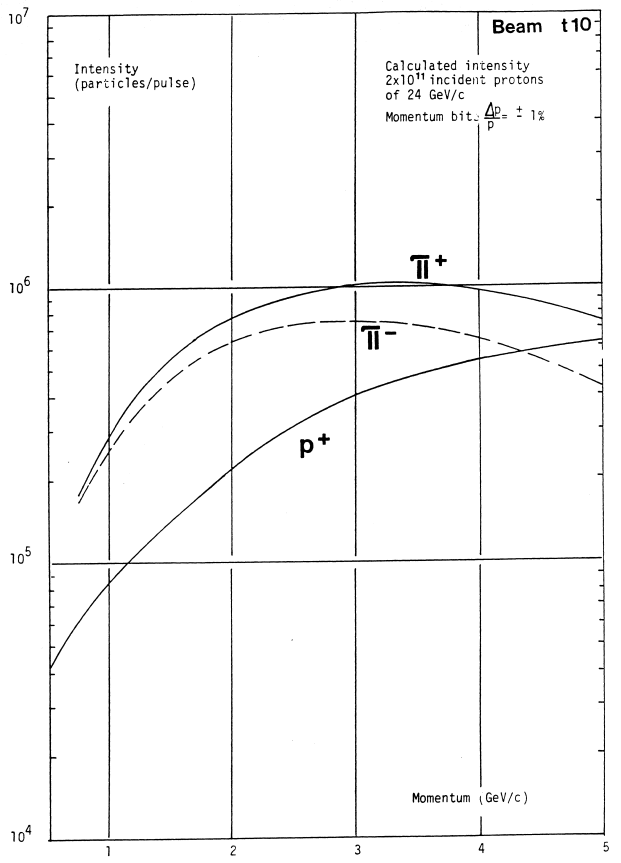
\includegraphics[width=.6\linewidth]{files/Figures/t10Comp.png}
  \caption{Calculated intensity of the T10 beam as a function of selected beam momentum, separated by particle type~\cite{T10Report}.}
  \label{fig:beamComp}
\end{figure}

\begin{figure}
  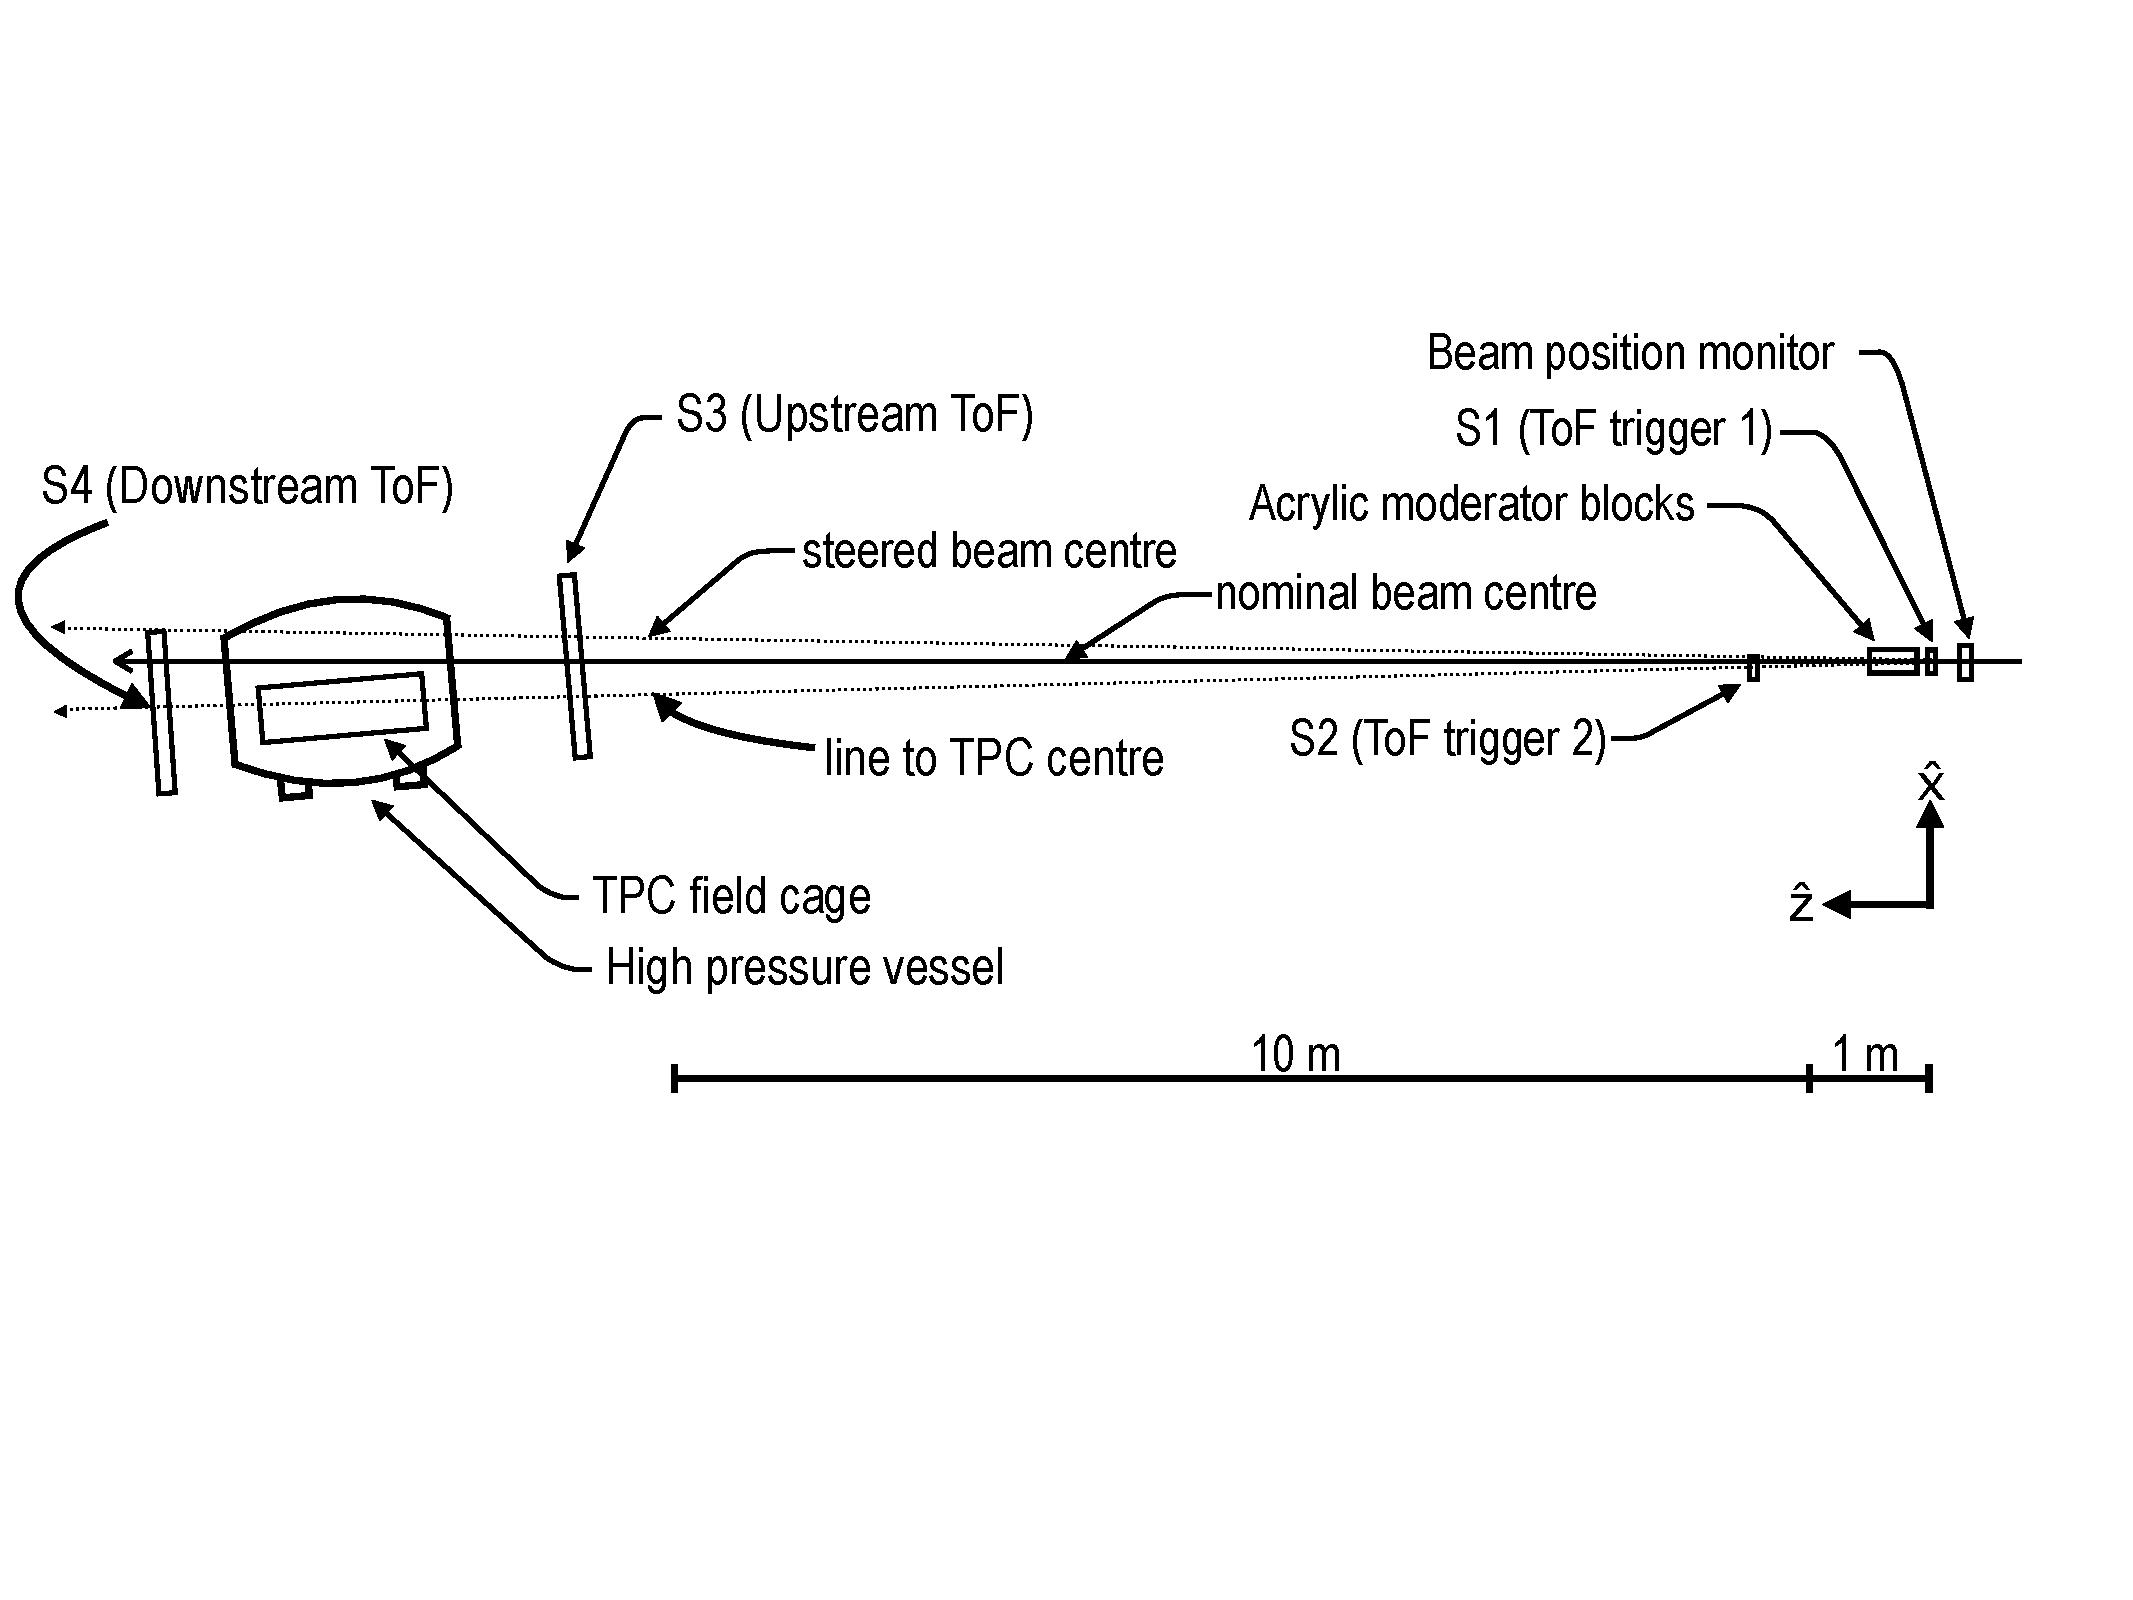
\includegraphics[width=1.0\linewidth]{files/Figures/hptpc_t10_planview.pdf}
  \caption{Schematic diagram (plan view) of the HPTPC beam test configuration in the T10 area at CERN.}
  \label{fig:setup}
\end{figure}
\begin{figure}
  \centering
  \includegraphics[width=1.0\linewidth]{files/Figures/S1S2S3S4.png}
  \caption{Photos illustrating the ToF constituents. Left: the downstream part of the setup which shows the $\mathit{S3}$, $\mathit{S4}$ detectors and HPTPC. Right: $\mathit{S1}$ and $\mathit{S2}$ counters and the stand with four acrylic moderator blocks.}
  \label{fig:modblocks}
\end{figure}

A beam position monitor (BPM) was situated at the beam entrance into the test area, upstream of all the ToF constituents and the TPC. 
The TPC was placed 13~m downstream of the BPM. 
From initial GEANT4~\cite{brun1993geant} beam simulations, the optimal TPC position to reduce the momentum of particles reaching the detector, without excessively reducing particle flux, was determined to be between 2$^{ \circ }$ and 3$^{ \circ }$ off the beam axis, but space constraints meant the TPC could not be placed that far away from the nominal beam centre. So, the beam was steered approximately 1$^{ \circ }$ away from its nominal position, and the TPC placed 1.5$^{ \circ }$ away from the nominal beam centre so that the TPC active region subtended an off-axis angular range of 1.4--3.8$^{ \circ }$.

There were four ToF constituents: 
\begin{itemize}
    \item $\mathit{S1}$, a small-area beam trigger, see Section~\ref{subsec:s1s2Exp};
    \item $\mathit{S2}$, a coincidence measurement with $\mathit{S1}$, see Section~\ref{subsec:s1s2Exp};
    \item $\mathit{S3}$, a panel of plastic scintillator bars placed directly upstream of the TPC vessel, see Section~\ref{subsec:s3Exp};
    \item $\mathit{S4}$, a panel of plastic scintillator bars placed directly downstream of the TPC vessel, see Section~\ref{subsec:s4Exp}.
\end{itemize}

A series of acrylic (polymethyl methacrylate) blocks was placed between the $\mathit{S1}$ and $\mathit{S2}$ counters.
Up to four $10\times10\times10$~cm$^3$ acrylic blocks could be placed contiguously on a tripod stand.
Figure~\ref{fig:modblocks} shows the stand with four blocks installed.
The moderator blocks have the effect of both reducing the energies of incoming particles as well as changing their directions.
This tends to increase the proton-to-MIP ratio at low off-axis angles from the beam, while decreasing the total number of protons and MIPs traversing the TPC.
Data were collected with the T10 beam momentum setting at 0.8~GeV/c, and with each configuration of 0 to 4 moderator blocks.

%The ToF systems were placed in off-axis positions with respect to the direction of the beam to match the TPC position.
The data acquisition (DAQ) systems of the $\mathit{S3}$ (upstream) and $\mathit{S4}$ (downstream) ToF systems were completely independent.
Synchronization between ToF DAQ systems was performed offline using the reference signal from the PS at the beginning of every spill.
T10 received 1--3 spills from the PS during each supercycle, which has a typical duration of 33~s.
The spill duration is 400~ms.
The minimum separation in time between two spills is 1 second, so the start-of-spill signal frequency is less than or equal to 1~Hz.
The trigger condition of the upstream ToF was based on the coincidence between $\mathit{S1}$ and $\mathit{S3}$ constituents.
$\mathit{S2}$ signals were also recorded by the upstream ToF DAQ but were not used in the trigger.
The DAQ of the downstream ToF was run in self-triggering mode with a gate open during the spill.
Coincidence signals between $\mathit{S1}$ and $\mathit{S2}$ counters were also recorded by the downstream ToF DAQ and were used in the particle identification (PID) analysis, described in Section~\ref{hptpcPaper:sec:Results}.  

\subsection{Survey and coordinate system}
\label{sec:coord}
The T10 beamline area was surveyed, and the distances to specific components measured with a precision of 0.5~mm by the CERN Survey, Mechatronics and Measurements (SMM) group.
Multiple points on each of $\mathit{S1}$, $\mathit{S2}$, $\mathit{S3}$, $\mathit{S4}$ and the TPC frame have had their positions measured.

The axes of a right-handed coordinate system are defined as follows: $\hat{x}$ refers to the non-beam horizontal direction, $\hat{y}$ to the vertical direction, and $\hat{z}$ the beam direction, as shown in Figure~\ref{fig:setup}.
We show results in terms of two off-axis angles: $\theta$, which is measured in the $\hat{x}-\hat{z}$ plane with positive angles measured in the $+\hat{x}$ direction, and $\phi$, which is measured in the $\hat{y}-\hat{z}$ plane with positive angles measured in the $+\hat{y}$ direction.
The origin is taken to be at $\mathit{S1}$.

Figure~\ref{fig:angularDistS1} shows the angular extent of objects within the beamline using the coordinate system defined above.
Table~\ref{tab:angS1} shows the calculated angular extent of the various beamline components as measured from $\mathit{S1}$.
Table~\ref{tab:distances} shows the distances between the centres of various objects in the T10 beamline.
These distances were calculated using the data gathered by the survey team.

\begin{figure}[ht]
  \begin{adjustbox}{max totalsize={0.7\textwidth}{.5\textheight},center}
    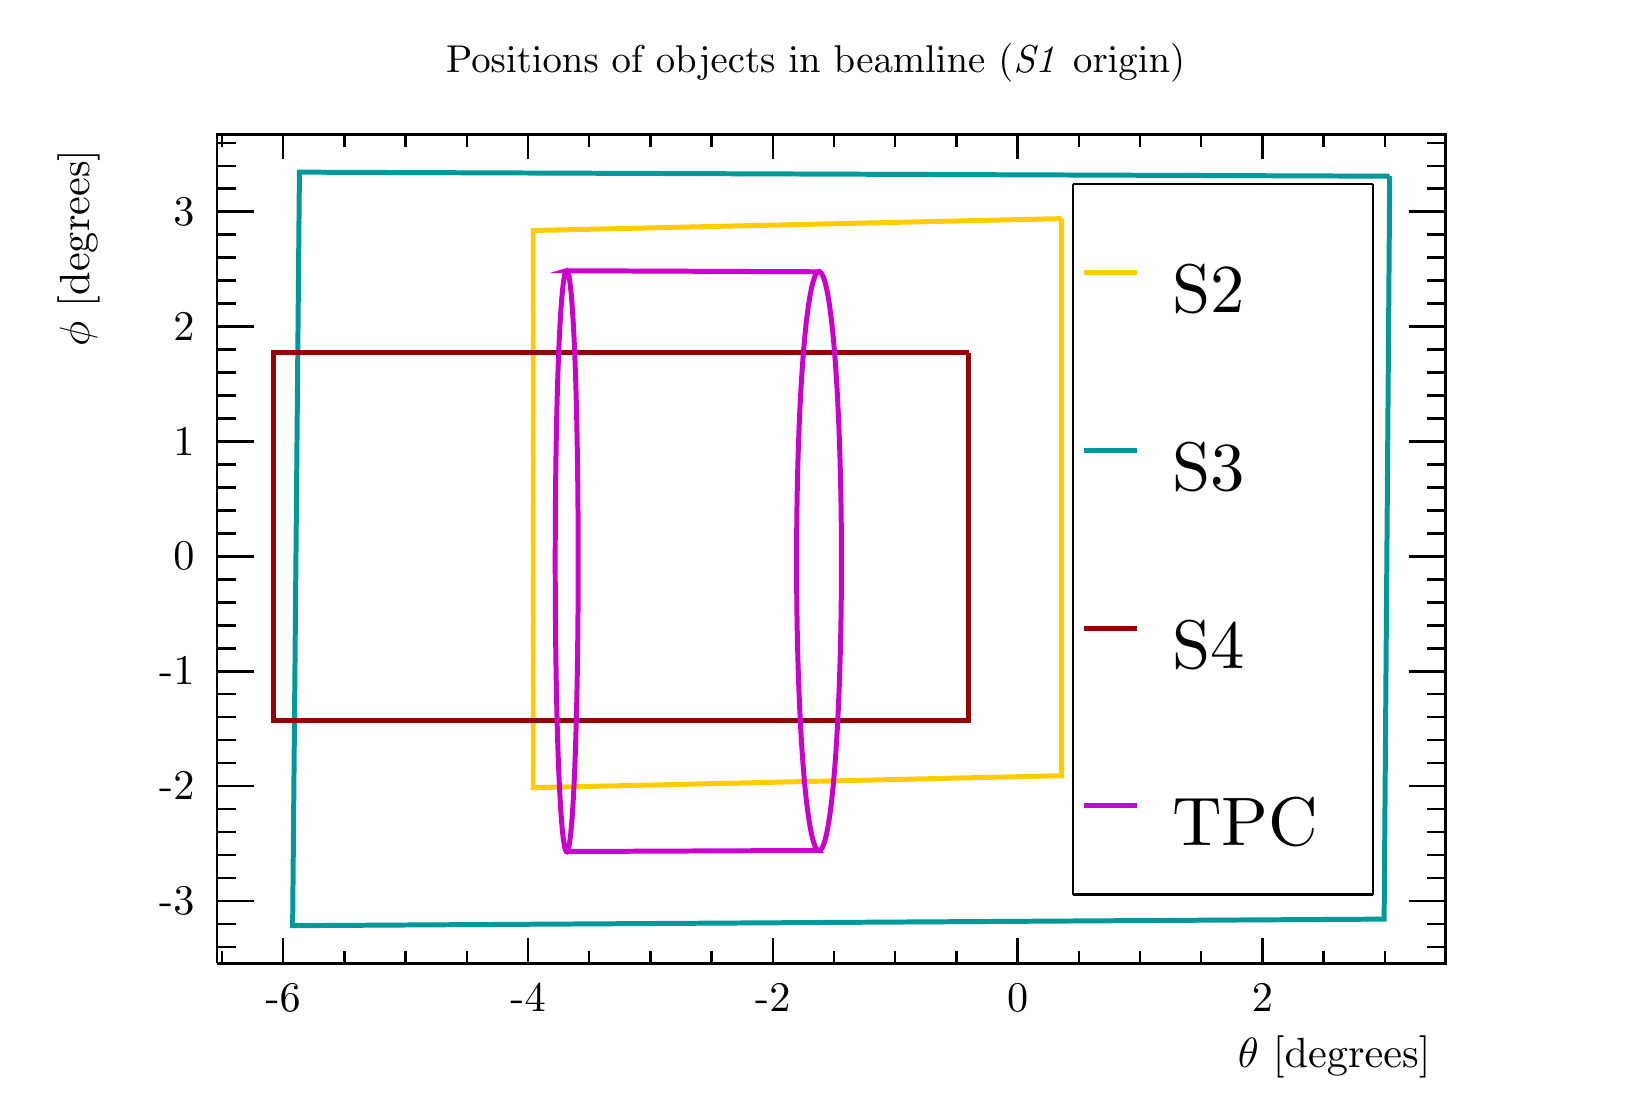
\begin{tikzpicture}
\pgfdeclareplotmark{cross} {
\pgfpathmoveto{\pgfpoint{-0.3\pgfplotmarksize}{\pgfplotmarksize}}
\pgfpathlineto{\pgfpoint{+0.3\pgfplotmarksize}{\pgfplotmarksize}}
\pgfpathlineto{\pgfpoint{+0.3\pgfplotmarksize}{0.3\pgfplotmarksize}}
\pgfpathlineto{\pgfpoint{+1\pgfplotmarksize}{0.3\pgfplotmarksize}}
\pgfpathlineto{\pgfpoint{+1\pgfplotmarksize}{-0.3\pgfplotmarksize}}
\pgfpathlineto{\pgfpoint{+0.3\pgfplotmarksize}{-0.3\pgfplotmarksize}}
\pgfpathlineto{\pgfpoint{+0.3\pgfplotmarksize}{-1.\pgfplotmarksize}}
\pgfpathlineto{\pgfpoint{-0.3\pgfplotmarksize}{-1.\pgfplotmarksize}}
\pgfpathlineto{\pgfpoint{-0.3\pgfplotmarksize}{-0.3\pgfplotmarksize}}
\pgfpathlineto{\pgfpoint{-1.\pgfplotmarksize}{-0.3\pgfplotmarksize}}
\pgfpathlineto{\pgfpoint{-1.\pgfplotmarksize}{0.3\pgfplotmarksize}}
\pgfpathlineto{\pgfpoint{-0.3\pgfplotmarksize}{0.3\pgfplotmarksize}}
\pgfpathclose
\pgfusepathqstroke
}
\pgfdeclareplotmark{cross*} {
\pgfpathmoveto{\pgfpoint{-0.3\pgfplotmarksize}{\pgfplotmarksize}}
\pgfpathlineto{\pgfpoint{+0.3\pgfplotmarksize}{\pgfplotmarksize}}
\pgfpathlineto{\pgfpoint{+0.3\pgfplotmarksize}{0.3\pgfplotmarksize}}
\pgfpathlineto{\pgfpoint{+1\pgfplotmarksize}{0.3\pgfplotmarksize}}
\pgfpathlineto{\pgfpoint{+1\pgfplotmarksize}{-0.3\pgfplotmarksize}}
\pgfpathlineto{\pgfpoint{+0.3\pgfplotmarksize}{-0.3\pgfplotmarksize}}
\pgfpathlineto{\pgfpoint{+0.3\pgfplotmarksize}{-1.\pgfplotmarksize}}
\pgfpathlineto{\pgfpoint{-0.3\pgfplotmarksize}{-1.\pgfplotmarksize}}
\pgfpathlineto{\pgfpoint{-0.3\pgfplotmarksize}{-0.3\pgfplotmarksize}}
\pgfpathlineto{\pgfpoint{-1.\pgfplotmarksize}{-0.3\pgfplotmarksize}}
\pgfpathlineto{\pgfpoint{-1.\pgfplotmarksize}{0.3\pgfplotmarksize}}
\pgfpathlineto{\pgfpoint{-0.3\pgfplotmarksize}{0.3\pgfplotmarksize}}
\pgfpathclose
\pgfusepathqfillstroke
}
\pgfdeclareplotmark{newstar} {
\pgfpathmoveto{\pgfqpoint{0pt}{\pgfplotmarksize}}
\pgfpathlineto{\pgfqpointpolar{44}{0.5\pgfplotmarksize}}
\pgfpathlineto{\pgfqpointpolar{18}{\pgfplotmarksize}}
\pgfpathlineto{\pgfqpointpolar{-20}{0.5\pgfplotmarksize}}
\pgfpathlineto{\pgfqpointpolar{-54}{\pgfplotmarksize}}
\pgfpathlineto{\pgfqpointpolar{-90}{0.5\pgfplotmarksize}}
\pgfpathlineto{\pgfqpointpolar{234}{\pgfplotmarksize}}
\pgfpathlineto{\pgfqpointpolar{198}{0.5\pgfplotmarksize}}
\pgfpathlineto{\pgfqpointpolar{162}{\pgfplotmarksize}}
\pgfpathlineto{\pgfqpointpolar{134}{0.5\pgfplotmarksize}}
\pgfpathclose
\pgfusepathqstroke
}
\pgfdeclareplotmark{newstar*} {
\pgfpathmoveto{\pgfqpoint{0pt}{\pgfplotmarksize}}
\pgfpathlineto{\pgfqpointpolar{44}{0.5\pgfplotmarksize}}
\pgfpathlineto{\pgfqpointpolar{18}{\pgfplotmarksize}}
\pgfpathlineto{\pgfqpointpolar{-20}{0.5\pgfplotmarksize}}
\pgfpathlineto{\pgfqpointpolar{-54}{\pgfplotmarksize}}
\pgfpathlineto{\pgfqpointpolar{-90}{0.5\pgfplotmarksize}}
\pgfpathlineto{\pgfqpointpolar{234}{\pgfplotmarksize}}
\pgfpathlineto{\pgfqpointpolar{198}{0.5\pgfplotmarksize}}
\pgfpathlineto{\pgfqpointpolar{162}{\pgfplotmarksize}}
\pgfpathlineto{\pgfqpointpolar{134}{0.5\pgfplotmarksize}}
\pgfpathclose
\pgfusepathqfillstroke
}
\definecolor{c}{rgb}{1,1,1};
\draw [color=c, fill=c] (0,0) rectangle (20,13.4957);
\draw [color=c, fill=c] (2.4,1.61948) rectangle (18,12.1461);
\definecolor{c}{rgb}{0,0,0};
\draw [c,line width=0.9] (2.4,1.61948) -- (2.4,12.1461) -- (18,12.1461) -- (18,1.61948) -- (2.4,1.61948);
\definecolor{c}{rgb}{1,1,1};
\draw [color=c, fill=c] (2.4,1.61948) rectangle (18,12.1461);
\definecolor{c}{rgb}{0,0,0};
\draw [c,line width=0.9] (2.4,1.61948) -- (2.4,12.1461) -- (18,12.1461) -- (18,1.61948) -- (2.4,1.61948);
\draw [c,line width=0.9] (2.4,1.61948) -- (18,1.61948);
\draw [c,line width=0.9] (3.23864,1.93528) -- (3.23864,1.61948);
\draw [c,line width=0.9] (4.01586,1.77738) -- (4.01586,1.61948);
\draw [c,line width=0.9] (4.79308,1.77738) -- (4.79308,1.61948);
\draw [c,line width=0.9] (5.5703,1.77738) -- (5.5703,1.61948);
\draw [c,line width=0.9] (6.34753,1.93528) -- (6.34753,1.61948);
\draw [c,line width=0.9] (7.12475,1.77738) -- (7.12475,1.61948);
\draw [c,line width=0.9] (7.90197,1.77738) -- (7.90197,1.61948);
\draw [c,line width=0.9] (8.67919,1.77738) -- (8.67919,1.61948);
\draw [c,line width=0.9] (9.45641,1.93528) -- (9.45641,1.61948);
\draw [c,line width=0.9] (10.2336,1.77738) -- (10.2336,1.61948);
\draw [c,line width=0.9] (11.0109,1.77738) -- (11.0109,1.61948);
\draw [c,line width=0.9] (11.7881,1.77738) -- (11.7881,1.61948);
\draw [c,line width=0.9] (12.5653,1.93528) -- (12.5653,1.61948);
\draw [c,line width=0.9] (13.3425,1.77738) -- (13.3425,1.61948);
\draw [c,line width=0.9] (14.1197,1.77738) -- (14.1197,1.61948);
\draw [c,line width=0.9] (14.897,1.77738) -- (14.897,1.61948);
\draw [c,line width=0.9] (15.6742,1.93528) -- (15.6742,1.61948);
\draw [c,line width=0.9] (3.23864,1.93528) -- (3.23864,1.61948);
\draw [c,line width=0.9] (2.46142,1.77738) -- (2.46142,1.61948);
\draw [c,line width=0.9] (15.6742,1.93528) -- (15.6742,1.61948);
\draw [c,line width=0.9] (16.4514,1.77738) -- (16.4514,1.61948);
\draw [c,line width=0.9] (17.2286,1.77738) -- (17.2286,1.61948);
\draw [anchor=base] (3.23864,1.01218) node[scale=1.52731, color=c, rotate=0]{-6};
\draw [anchor=base] (6.34753,1.01218) node[scale=1.52731, color=c, rotate=0]{-4};
\draw [anchor=base] (9.45641,1.01218) node[scale=1.52731, color=c, rotate=0]{-2};
\draw [anchor=base] (12.5653,1.01218) node[scale=1.52731, color=c, rotate=0]{0};
\draw [anchor=base] (15.6742,1.01218) node[scale=1.52731, color=c, rotate=0]{2};
\draw [anchor= east] (18,0.431862) node[scale=1.52731, color=c, rotate=0]{$ \theta$ [degrees]};
\draw [c,line width=0.9] (2.4,12.1461) -- (18,12.1461);
\draw [c,line width=0.9] (3.23864,11.8303) -- (3.23864,12.1461);
\draw [c,line width=0.9] (4.01586,11.9882) -- (4.01586,12.1461);
\draw [c,line width=0.9] (4.79308,11.9882) -- (4.79308,12.1461);
\draw [c,line width=0.9] (5.5703,11.9882) -- (5.5703,12.1461);
\draw [c,line width=0.9] (6.34753,11.8303) -- (6.34753,12.1461);
\draw [c,line width=0.9] (7.12475,11.9882) -- (7.12475,12.1461);
\draw [c,line width=0.9] (7.90197,11.9882) -- (7.90197,12.1461);
\draw [c,line width=0.9] (8.67919,11.9882) -- (8.67919,12.1461);
\draw [c,line width=0.9] (9.45641,11.8303) -- (9.45641,12.1461);
\draw [c,line width=0.9] (10.2336,11.9882) -- (10.2336,12.1461);
\draw [c,line width=0.9] (11.0109,11.9882) -- (11.0109,12.1461);
\draw [c,line width=0.9] (11.7881,11.9882) -- (11.7881,12.1461);
\draw [c,line width=0.9] (12.5653,11.8303) -- (12.5653,12.1461);
\draw [c,line width=0.9] (13.3425,11.9882) -- (13.3425,12.1461);
\draw [c,line width=0.9] (14.1197,11.9882) -- (14.1197,12.1461);
\draw [c,line width=0.9] (14.897,11.9882) -- (14.897,12.1461);
\draw [c,line width=0.9] (15.6742,11.8303) -- (15.6742,12.1461);
\draw [c,line width=0.9] (3.23864,11.8303) -- (3.23864,12.1461);
\draw [c,line width=0.9] (2.46142,11.9882) -- (2.46142,12.1461);
\draw [c,line width=0.9] (15.6742,11.8303) -- (15.6742,12.1461);
\draw [c,line width=0.9] (16.4514,11.9882) -- (16.4514,12.1461);
\draw [c,line width=0.9] (17.2286,11.9882) -- (17.2286,12.1461);
\draw [c,line width=0.9] (2.4,1.61948) -- (2.4,12.1461);
\draw [c,line width=0.9] (2.868,2.41096) -- (2.4,2.41096);
\draw [c,line width=0.9] (2.634,2.70278) -- (2.4,2.70278);
\draw [c,line width=0.9] (2.634,2.99459) -- (2.4,2.99459);
\draw [c,line width=0.9] (2.634,3.28641) -- (2.4,3.28641);
\draw [c,line width=0.9] (2.634,3.57822) -- (2.4,3.57822);
\draw [c,line width=0.9] (2.868,3.87004) -- (2.4,3.87004);
\draw [c,line width=0.9] (2.634,4.16185) -- (2.4,4.16185);
\draw [c,line width=0.9] (2.634,4.45367) -- (2.4,4.45367);
\draw [c,line width=0.9] (2.634,4.74548) -- (2.4,4.74548);
\draw [c,line width=0.9] (2.634,5.0373) -- (2.4,5.0373);
\draw [c,line width=0.9] (2.868,5.32911) -- (2.4,5.32911);
\draw [c,line width=0.9] (2.634,5.62093) -- (2.4,5.62093);
\draw [c,line width=0.9] (2.634,5.91274) -- (2.4,5.91274);
\draw [c,line width=0.9] (2.634,6.20456) -- (2.4,6.20456);
\draw [c,line width=0.9] (2.634,6.49638) -- (2.4,6.49638);
\draw [c,line width=0.9] (2.868,6.78819) -- (2.4,6.78819);
\draw [c,line width=0.9] (2.634,7.08001) -- (2.4,7.08001);
\draw [c,line width=0.9] (2.634,7.37182) -- (2.4,7.37182);
\draw [c,line width=0.9] (2.634,7.66364) -- (2.4,7.66364);
\draw [c,line width=0.9] (2.634,7.95545) -- (2.4,7.95545);
\draw [c,line width=0.9] (2.868,8.24727) -- (2.4,8.24727);
\draw [c,line width=0.9] (2.634,8.53908) -- (2.4,8.53908);
\draw [c,line width=0.9] (2.634,8.8309) -- (2.4,8.8309);
\draw [c,line width=0.9] (2.634,9.12271) -- (2.4,9.12271);
\draw [c,line width=0.9] (2.634,9.41453) -- (2.4,9.41453);
\draw [c,line width=0.9] (2.868,9.70634) -- (2.4,9.70634);
\draw [c,line width=0.9] (2.634,9.99816) -- (2.4,9.99816);
\draw [c,line width=0.9] (2.634,10.29) -- (2.4,10.29);
\draw [c,line width=0.9] (2.634,10.5818) -- (2.4,10.5818);
\draw [c,line width=0.9] (2.634,10.8736) -- (2.4,10.8736);
\draw [c,line width=0.9] (2.868,11.1654) -- (2.4,11.1654);
\draw [c,line width=0.9] (2.868,2.41096) -- (2.4,2.41096);
\draw [c,line width=0.9] (2.634,2.11915) -- (2.4,2.11915);
\draw [c,line width=0.9] (2.634,1.82733) -- (2.4,1.82733);
\draw [c,line width=0.9] (2.868,11.1654) -- (2.4,11.1654);
\draw [c,line width=0.9] (2.634,11.4572) -- (2.4,11.4572);
\draw [c,line width=0.9] (2.634,11.749) -- (2.4,11.749);
\draw [c,line width=0.9] (2.634,12.0409) -- (2.4,12.0409);
\draw [anchor= east] (2.3,2.41096) node[scale=1.52731, color=c, rotate=0]{-3};
\draw [anchor= east] (2.3,3.87004) node[scale=1.52731, color=c, rotate=0]{-2};
\draw [anchor= east] (2.3,5.32911) node[scale=1.52731, color=c, rotate=0]{-1};
\draw [anchor= east] (2.3,6.78819) node[scale=1.52731, color=c, rotate=0]{0};
\draw [anchor= east] (2.3,8.24727) node[scale=1.52731, color=c, rotate=0]{1};
\draw [anchor= east] (2.3,9.70634) node[scale=1.52731, color=c, rotate=0]{2};
\draw [anchor= east] (2.3,11.1654) node[scale=1.52731, color=c, rotate=0]{3};
\draw [anchor= east] (0.64,12.1461) node[scale=1.52731, color=c, rotate=90]{$ \phi$ [degrees]};
\draw [c,line width=0.9] (18,1.61948) -- (18,12.1461);
\draw [c,line width=0.9] (17.532,2.41096) -- (18,2.41096);
\draw [c,line width=0.9] (17.766,2.70278) -- (18,2.70278);
\draw [c,line width=0.9] (17.766,2.99459) -- (18,2.99459);
\draw [c,line width=0.9] (17.766,3.28641) -- (18,3.28641);
\draw [c,line width=0.9] (17.766,3.57822) -- (18,3.57822);
\draw [c,line width=0.9] (17.532,3.87004) -- (18,3.87004);
\draw [c,line width=0.9] (17.766,4.16185) -- (18,4.16185);
\draw [c,line width=0.9] (17.766,4.45367) -- (18,4.45367);
\draw [c,line width=0.9] (17.766,4.74548) -- (18,4.74548);
\draw [c,line width=0.9] (17.766,5.0373) -- (18,5.0373);
\draw [c,line width=0.9] (17.532,5.32911) -- (18,5.32911);
\draw [c,line width=0.9] (17.766,5.62093) -- (18,5.62093);
\draw [c,line width=0.9] (17.766,5.91274) -- (18,5.91274);
\draw [c,line width=0.9] (17.766,6.20456) -- (18,6.20456);
\draw [c,line width=0.9] (17.766,6.49638) -- (18,6.49638);
\draw [c,line width=0.9] (17.532,6.78819) -- (18,6.78819);
\draw [c,line width=0.9] (17.766,7.08001) -- (18,7.08001);
\draw [c,line width=0.9] (17.766,7.37182) -- (18,7.37182);
\draw [c,line width=0.9] (17.766,7.66364) -- (18,7.66364);
\draw [c,line width=0.9] (17.766,7.95545) -- (18,7.95545);
\draw [c,line width=0.9] (17.532,8.24727) -- (18,8.24727);
\draw [c,line width=0.9] (17.766,8.53908) -- (18,8.53908);
\draw [c,line width=0.9] (17.766,8.8309) -- (18,8.8309);
\draw [c,line width=0.9] (17.766,9.12271) -- (18,9.12271);
\draw [c,line width=0.9] (17.766,9.41453) -- (18,9.41453);
\draw [c,line width=0.9] (17.532,9.70634) -- (18,9.70634);
\draw [c,line width=0.9] (17.766,9.99816) -- (18,9.99816);
\draw [c,line width=0.9] (17.766,10.29) -- (18,10.29);
\draw [c,line width=0.9] (17.766,10.5818) -- (18,10.5818);
\draw [c,line width=0.9] (17.766,10.8736) -- (18,10.8736);
\draw [c,line width=0.9] (17.532,11.1654) -- (18,11.1654);
\draw [c,line width=0.9] (17.532,2.41096) -- (18,2.41096);
\draw [c,line width=0.9] (17.766,2.11915) -- (18,2.11915);
\draw [c,line width=0.9] (17.766,1.82733) -- (18,1.82733);
\draw [c,line width=0.9] (17.532,11.1654) -- (18,11.1654);
\draw [c,line width=0.9] (17.766,11.4572) -- (18,11.4572);
\draw [c,line width=0.9] (17.766,11.749) -- (18,11.749);
\draw [c,line width=0.9] (17.766,12.0409) -- (18,12.0409);
\definecolor{c}{rgb}{1,0.8,0};
\draw [c,line width=1.8] (13.123,11.0775) -- (13.123,4.00254) -- (6.41361,3.85009) -- (6.41361,10.9264) -- (13.123,11.0775);
\definecolor{c}{rgb}{0,0.6,0.6};
\draw [c,line width=1.8] (17.2909,11.6163) -- (3.44422,11.6676) -- (3.35799,2.09797) -- (17.22,2.18131) -- (17.2909,11.6163);
\definecolor{c}{rgb}{0.6,0,0};
\draw [c,line width=1.8] (11.9426,9.37206) -- (3.10909,9.37206) -- (3.10909,4.70729) -- (11.9426,4.70729) -- (11.9426,9.37206);
\definecolor{c}{rgb}{0.8,0,0.8};
\draw [c,line width=1.8] (6.83226,10.4157) -- (6.82314,10.3986) -- (6.81412,10.3672) -- (6.80521,10.3217) -- (6.79645,10.2624) -- (6.78788,10.1897) -- (6.77953,10.104) -- (6.77142,10.0055) -- (6.76359,9.89494) -- (6.75605,9.77263) --
 (6.74885,9.63914) -- (6.74199,9.49505) -- (6.73552,9.34093) -- (6.72943,9.17739) -- (6.72376,9.00508) -- (6.71852,8.82465) -- (6.71374,8.63678) -- (6.70941,8.44217) -- (6.70557,8.24152) -- (6.70221,8.03556) -- (6.69935,7.82503) -- (6.697,7.61067) --
 (6.69517,7.39324) -- (6.69385,7.17349) -- (6.69306,6.9522) -- (6.6928,6.73012) -- (6.69306,6.50804) -- (6.69385,6.28672) -- (6.69517,6.06693) -- (6.697,5.84944) -- (6.69935,5.635) -- (6.70221,5.42438) -- (6.70557,5.21831) -- (6.70941,5.01753) --
 (6.71374,4.82277) -- (6.71852,4.63474) -- (6.72376,4.45413) -- (6.72943,4.28163) -- (6.73552,4.11789) -- (6.74199,3.96355) -- (6.74885,3.81922) -- (6.75605,3.68549) -- (6.76359,3.56292) -- (6.77142,3.45203) -- (6.77953,3.35333) -- (6.78788,3.26727)
 -- (6.79645,3.19426) -- (6.80521,3.13469) -- (6.81412,3.08889) -- (6.82314,3.05715) -- (6.83226,3.0397) -- (6.84142,3.03673) -- (6.8506,3.04837) -- (6.85976,3.07469) -- (6.86885,3.11572) -- (6.87785,3.17139) -- (6.88671,3.24161) -- (6.8954,3.3262)
 -- (6.90388,3.42493) -- (6.91211,3.53747) -- (6.92006,3.66348) -- (6.92769,3.80249) -- (6.93496,3.95402) -- (6.94184,4.11749) -- (6.9483,4.29226) -- (6.95431,4.47764) -- (6.95985,4.67288) -- (6.96487,4.87717) -- (6.96936,5.08963) -- (6.9733,5.30937)
 -- (6.97667,5.53544) -- (6.97945,5.76682) -- (6.98163,6.00252) -- (6.98319,6.24147) -- (6.98413,6.4826) -- (6.98444,6.72484) -- (6.98413,6.96709) -- (6.98319,7.20826) -- (6.98163,7.44728) -- (6.97945,7.68305) -- (6.97667,7.91455) -- (6.9733,8.14075)
 -- (6.96936,8.36064) -- (6.96487,8.57329) -- (6.95985,8.77777) -- (6.95431,8.97322) -- (6.9483,9.15884) -- (6.94184,9.33386) -- (6.93496,9.49759) -- (6.92769,9.6494) -- (6.92006,9.7887) -- (6.91211,9.91501) -- (6.90388,10.0279) -- (6.8954,10.1269)
 -- (6.88671,10.2118) -- (6.87785,10.2824) -- (6.86885,10.3384) -- (6.85976,10.3797) -- (6.8506,10.4064) -- (6.84142,10.4184) -- (6.83226,10.4157) -- (10.0306,10.4025);
\draw [c,line width=1.8] (10.0306,3.05337) -- (10.0485,3.05045) -- (10.0665,3.06209) -- (10.0843,3.08835) -- (10.1021,3.12926) -- (10.1197,3.18477) -- (10.137,3.25476) -- (10.154,3.33907) -- (10.1705,3.43746) -- (10.1866,3.54962) -- (10.2022,3.67518)
 -- (10.2171,3.8137) -- (10.2313,3.96468) -- (10.2447,4.12756) -- (10.2573,4.30169) -- (10.2691,4.48639) -- (10.2799,4.6809) -- (10.2897,4.88442) -- (10.2985,5.09609) -- (10.3062,5.315) -- (10.3127,5.54021) -- (10.3182,5.77072) -- (10.3224,6.00552)
 -- (10.3255,6.24356) -- (10.3273,6.48377) -- (10.3279,6.72508) -- (10.3273,6.96641) -- (10.3255,7.20666) -- (10.3224,7.44476) -- (10.3182,7.67964) -- (10.3127,7.91026) -- (10.3062,8.1356) -- (10.2985,8.35466) -- (10.2897,8.56651) --
 (10.2799,8.77022) -- (10.2691,8.96495) -- (10.2573,9.14988) -- (10.2447,9.32426) -- (10.2313,9.4874) -- (10.2171,9.63865) -- (10.2022,9.77747) -- (10.1866,9.90332) -- (10.1705,10.0158) -- (10.154,10.1145) -- (10.137,10.1991) -- (10.1197,10.2695) --
 (10.1021,10.3253) -- (10.0843,10.3665) -- (10.0665,10.3931) -- (10.0485,10.4051) -- (10.0306,10.4025) -- (10.0128,10.3855) -- (9.99516,10.3542) -- (9.97776,10.3089) -- (9.96065,10.2499) -- (9.9439,10.1775) -- (9.92757,10.0921) -- (9.91173,9.99402)
 -- (9.89642,9.88383) -- (9.8817,9.76198) -- (9.86762,9.62899) -- (9.85423,9.48543) -- (9.84156,9.33188) -- (9.82967,9.16894) -- (9.81859,8.99725) -- (9.80836,8.81747) -- (9.799,8.63027) -- (9.79055,8.43635) -- (9.78303,8.23641) -- (9.77647,8.03118)
 -- (9.77088,7.82139) -- (9.76629,7.60779) -- (9.7627,7.39112) -- (9.76013,7.17214) -- (9.75859,6.95162) -- (9.75807,6.73033) -- (9.75859,6.50902) -- (9.76013,6.28848) -- (9.7627,6.06946) -- (9.76629,5.85273) -- (9.77088,5.63905) -- (9.77647,5.42916)
 -- (9.78303,5.22382) -- (9.79055,5.02376) -- (9.799,4.82969) -- (9.80836,4.64234) -- (9.81859,4.46238) -- (9.82967,4.2905) -- (9.84156,4.12736) -- (9.85423,3.97358) -- (9.86762,3.82979) -- (9.8817,3.69656) -- (9.89642,3.57445) -- (9.91173,3.46399)
 -- (9.92757,3.36567) -- (9.9439,3.27994) -- (9.96065,3.20723) -- (9.97776,3.14791) -- (9.99516,3.10231) -- (10.0128,3.07072) -- (10.0306,3.05337) -- (6.83226,3.0397);
\definecolor{c}{rgb}{1,1,1};
\draw [color=c, fill=c] (2,12.686) rectangle (18,13.4282);
\definecolor{c}{rgb}{0,0,0};
\draw (10,13.0571) node[scale=1.40004, color=c, rotate=0]{Positions of objects in beamline ($\mathit{S1}$ origin)};
\definecolor{c}{rgb}{1,1,1};
\draw [color=c, fill=c] (13.2665,2.49284) rectangle (17.0774,11.5186);
\definecolor{c}{rgb}{0,0,0};
\draw [c,line width=0.9] (13.2665,2.49284) -- (17.0774,2.49284);
\draw [c,line width=0.9] (17.0774,2.49284) -- (17.0774,11.5186);
\draw [c,line width=0.9] (17.0774,11.5186) -- (13.2665,11.5186);
\draw [c,line width=0.9] (13.2665,11.5186) -- (13.2665,2.49284);
\draw [anchor=base west] (14.2192,9.8827) node[scale=2.48189, color=c, rotate=0]{S2};
\definecolor{c}{rgb}{1,0.8,0};
\draw [c,line width=1.8] (13.4094,10.3904) -- (14.0763,10.3904);
\definecolor{c}{rgb}{0,0,0};
\draw [anchor=base west] (14.2192,7.62625) node[scale=2.48189, color=c, rotate=0]{S3};
\definecolor{c}{rgb}{0,0.6,0.6};
\draw [c,line width=1.8] (13.4094,8.13395) -- (14.0763,8.13395);
\definecolor{c}{rgb}{0,0,0};
\draw [anchor=base west] (14.2192,5.36981) node[scale=2.48189, color=c, rotate=0]{S4};
\definecolor{c}{rgb}{0.6,0,0};
\draw [c,line width=1.8] (13.4094,5.87751) -- (14.0763,5.87751);
\definecolor{c}{rgb}{0,0,0};
\draw [anchor=base west] (14.2192,3.11336) node[scale=2.48189, color=c, rotate=0]{TPC};
\definecolor{c}{rgb}{0.8,0,0.8};
\draw [c,line width=1.8] (13.4094,3.62106) -- (14.0763,3.62106);
\end{tikzpicture}

  \end{adjustbox}
  \caption{Angular position of various objects within the T10 beamline. US and DS refer to the upstream and downstream faces of the HPTPC. The origin in this view is at the centre of $\mathit{S1}$; the true centre of the steered beam is at +1$^{\circ}$ in $\theta$ and 0$^{\circ}$ in $\phi$.}
  \label{fig:angularDistS1}
\end{figure}

\begin{table}
  \centering
  \caption{Angular extents of objects within the T10 beamline as measured from $\mathit{S1}$.}
  \begin{tabular}{c|c c c c}
    \hline
    \hline
    Object & Minimum $\theta$ & Maximum $\theta$ & Minimum $\phi$ & Maximum $\phi$ \\
    \hline
    $\mathit{S2}$ & $-3.96^{\circ} \pm 0.03^{\circ}$ & $0.36^{\circ} \pm 0.03^{\circ}$ & $-2.01^{\circ} \pm 0.03^{\circ}$ & $2.94^{\circ} \pm 0.03^{\circ}$ \\
    $\mathit{S3}$ & $-5.923^{\circ} \pm 0.004^{\circ}$ & \hspace{6pt} $3.040^{\circ} \pm 0.004^{\circ}$ & $-3.215^{\circ} \pm 0.004^{\circ}$ & $3.344^{\circ} \pm 0.004^{\circ}$ \\
   $\mathit{S4}$ & $-6.083^{\circ} \pm 0.003^{\circ}$ & $-0.401^{\circ} \pm 0.003^{\circ}$ & $-1.426^{\circ} \pm 0.003^{\circ}$ & $1.771^{\circ} \pm 0.003^{\circ}$ \\
    TPC upstream face & $-3.59^{\circ} \pm 0.01^{\circ}$ & $-1.44^{\circ} \pm 0.01^{\circ}$ & $-2.66^{\circ} \pm 0.01^{\circ}$ & $2.58^{\circ} \pm 0.01^{\circ}$ \\
    TPC downstream face & $-3.778^{\circ} \pm 0.009^{\circ}$ & $-1.806^{\circ} \pm 0.009^{\circ}$ & $-2.440^{\circ} \pm 0.009^{\circ}$ & $2.361^{\circ} \pm 0.009^{\circ}$ \\
    \hline
  \end{tabular}
  \label{tab:angS1}
\end{table}

\begin{table}
  \centering
  \caption{Distances between objects in the T10 beamline. US and DS refer to the upstream and downstream edges of the TPC, respectively.}
  \begin{tabular}{c|c}
    \hline
    \hline
    Points & Distance between centres / m\\
    \hline
    Beam monitor -- $\mathit{S1}$ & $0.288 \pm 0.001$ \\
    $\mathit{S1}-\mathit{S2}$ & $1.419 \pm 0.001$ \\
    $\mathit{S1}-\mathit{S3}$ & $10.756 \pm 0.001$ \\
    $\mathit{S3}$ -- TPC US side & $1.323 \pm 0.002$ \\
    TPC DS side -- $\mathit{S4}$ & $0.918 \pm 0.002$ \\
    $\mathit{S2}-\mathit{S4}$ & $12.651 \pm 0.001$ \\
    \hline    
  \end{tabular}
  \label{tab:distances}
\end{table}

\subsection{Upstream beam counters (S1 and S2)}
\label{subsec:s1s2Exp}
\begin{figure}
  \centering
  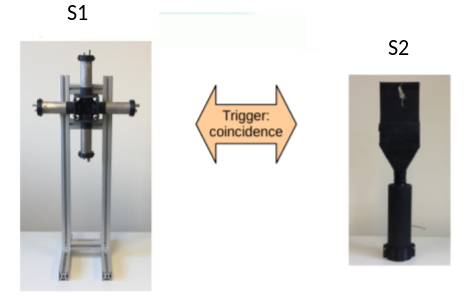
\includegraphics[width=0.7\linewidth]{files/Figures/S1S2FrontOn.png}
  \caption{The S1 and S2 beam counters. Together the coincidence of signals in the beam counters were recorded by the DAQ systems.}
  \label{fig:S1S2headon}
\end{figure}
The beam counters $\mathit{S1}$ and $\mathit{S2}$ are shown in Figure~\ref{fig:S1S2headon}.
The $\mathit{S1}$ counter is a $40\times40\times5$~mm$^3$ plastic scintillator cross which is attached to four 1'' Hamamatsu Photonics R4998 photomultiplier tubes (PMTs) at each end for the light readout.
The time resolution of the counter, as measured by the DAQ system of the upstream ToF, was about 30~ps. This is estimated with the distribution of the average PMT hit times; the quantity $t_{\textrm{ave}}=\frac{1}{4}((t_{\textrm{PMT0}}+t_{\textrm{PMT1}})-(t_{\textrm{PMT2}}+t_{\textrm{PMT3}}))$ has the same spread as the simple average but is conveniently centered at zero.
An example of the $t_{\textrm{ave}}$ distribution for one run of $\mathit{S1}$ data is shown in Figure~\ref{fig:s1Res}. The full width at half maximum (FWHM) of the distribution is 62 ps.

\begin{figure}
  \begin{adjustbox}{width=0.7\linewidth, center}
    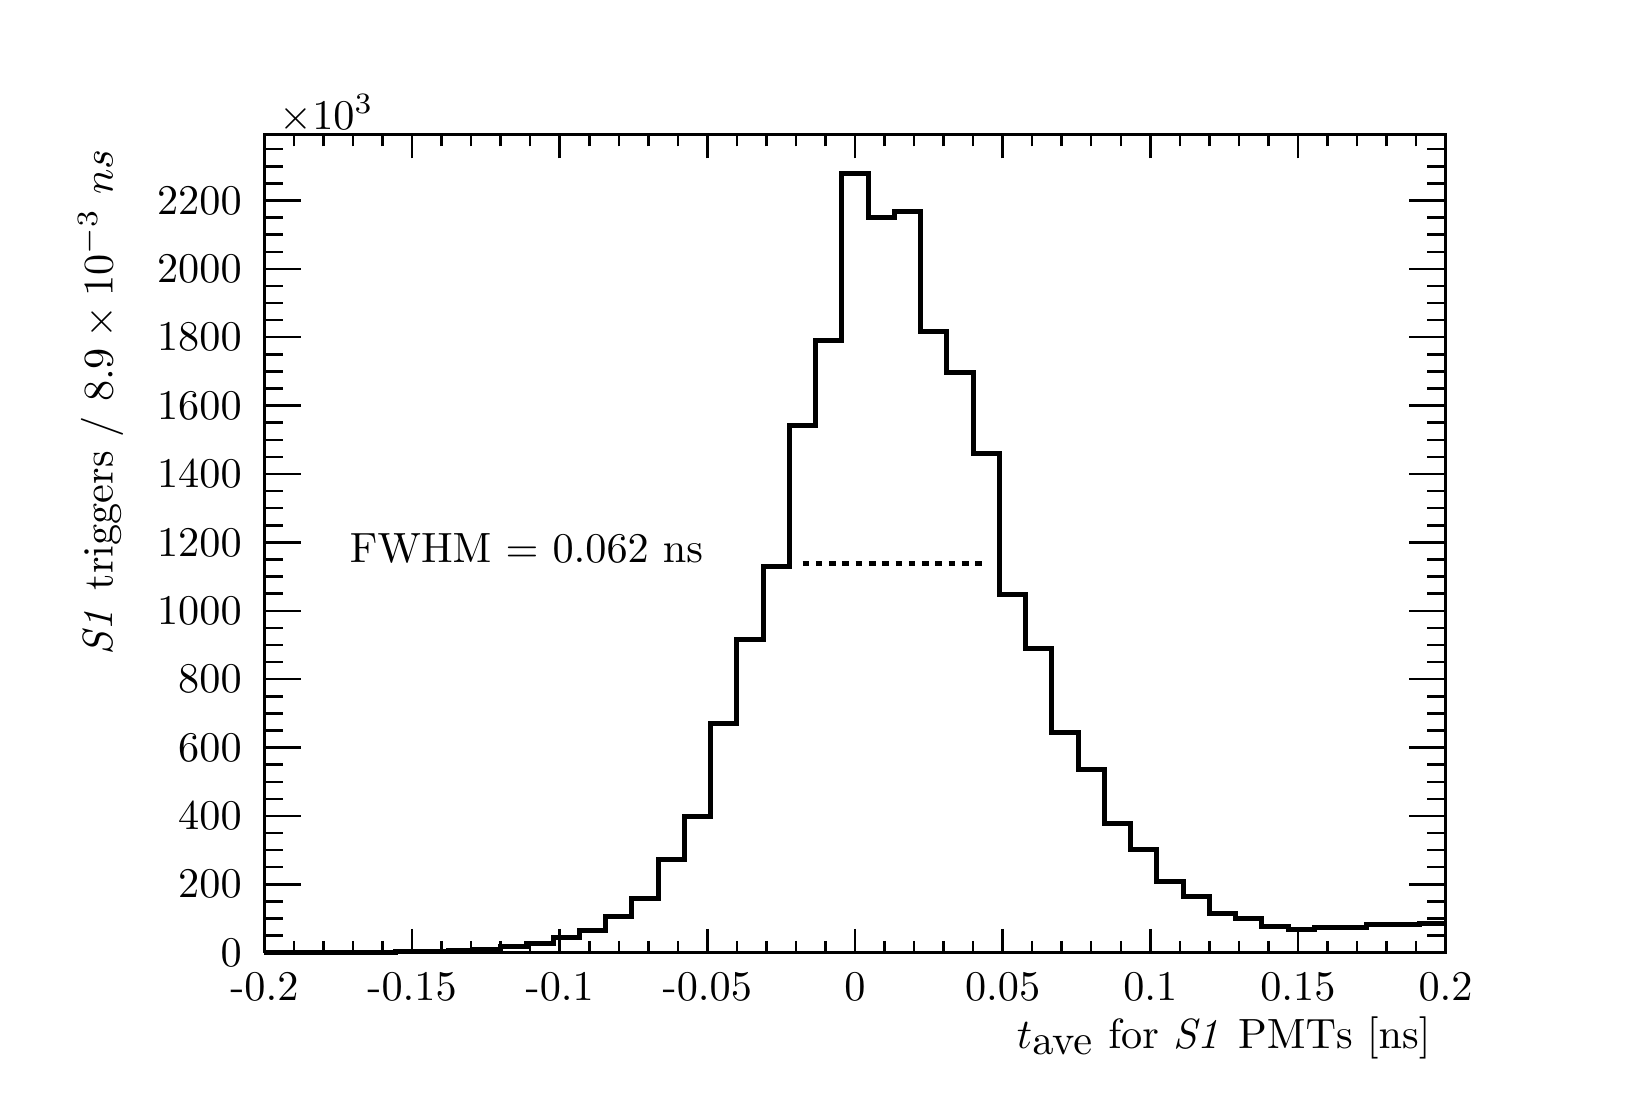
\begin{tikzpicture}
\pgfdeclareplotmark{cross} {
\pgfpathmoveto{\pgfpoint{-0.3\pgfplotmarksize}{\pgfplotmarksize}}
\pgfpathlineto{\pgfpoint{+0.3\pgfplotmarksize}{\pgfplotmarksize}}
\pgfpathlineto{\pgfpoint{+0.3\pgfplotmarksize}{0.3\pgfplotmarksize}}
\pgfpathlineto{\pgfpoint{+1\pgfplotmarksize}{0.3\pgfplotmarksize}}
\pgfpathlineto{\pgfpoint{+1\pgfplotmarksize}{-0.3\pgfplotmarksize}}
\pgfpathlineto{\pgfpoint{+0.3\pgfplotmarksize}{-0.3\pgfplotmarksize}}
\pgfpathlineto{\pgfpoint{+0.3\pgfplotmarksize}{-1.\pgfplotmarksize}}
\pgfpathlineto{\pgfpoint{-0.3\pgfplotmarksize}{-1.\pgfplotmarksize}}
\pgfpathlineto{\pgfpoint{-0.3\pgfplotmarksize}{-0.3\pgfplotmarksize}}
\pgfpathlineto{\pgfpoint{-1.\pgfplotmarksize}{-0.3\pgfplotmarksize}}
\pgfpathlineto{\pgfpoint{-1.\pgfplotmarksize}{0.3\pgfplotmarksize}}
\pgfpathlineto{\pgfpoint{-0.3\pgfplotmarksize}{0.3\pgfplotmarksize}}
\pgfpathclose
\pgfusepathqstroke
}
\pgfdeclareplotmark{cross*} {
\pgfpathmoveto{\pgfpoint{-0.3\pgfplotmarksize}{\pgfplotmarksize}}
\pgfpathlineto{\pgfpoint{+0.3\pgfplotmarksize}{\pgfplotmarksize}}
\pgfpathlineto{\pgfpoint{+0.3\pgfplotmarksize}{0.3\pgfplotmarksize}}
\pgfpathlineto{\pgfpoint{+1\pgfplotmarksize}{0.3\pgfplotmarksize}}
\pgfpathlineto{\pgfpoint{+1\pgfplotmarksize}{-0.3\pgfplotmarksize}}
\pgfpathlineto{\pgfpoint{+0.3\pgfplotmarksize}{-0.3\pgfplotmarksize}}
\pgfpathlineto{\pgfpoint{+0.3\pgfplotmarksize}{-1.\pgfplotmarksize}}
\pgfpathlineto{\pgfpoint{-0.3\pgfplotmarksize}{-1.\pgfplotmarksize}}
\pgfpathlineto{\pgfpoint{-0.3\pgfplotmarksize}{-0.3\pgfplotmarksize}}
\pgfpathlineto{\pgfpoint{-1.\pgfplotmarksize}{-0.3\pgfplotmarksize}}
\pgfpathlineto{\pgfpoint{-1.\pgfplotmarksize}{0.3\pgfplotmarksize}}
\pgfpathlineto{\pgfpoint{-0.3\pgfplotmarksize}{0.3\pgfplotmarksize}}
\pgfpathclose
\pgfusepathqfillstroke
}
\pgfdeclareplotmark{newstar} {
\pgfpathmoveto{\pgfqpoint{0pt}{\pgfplotmarksize}}
\pgfpathlineto{\pgfqpointpolar{44}{0.5\pgfplotmarksize}}
\pgfpathlineto{\pgfqpointpolar{18}{\pgfplotmarksize}}
\pgfpathlineto{\pgfqpointpolar{-20}{0.5\pgfplotmarksize}}
\pgfpathlineto{\pgfqpointpolar{-54}{\pgfplotmarksize}}
\pgfpathlineto{\pgfqpointpolar{-90}{0.5\pgfplotmarksize}}
\pgfpathlineto{\pgfqpointpolar{234}{\pgfplotmarksize}}
\pgfpathlineto{\pgfqpointpolar{198}{0.5\pgfplotmarksize}}
\pgfpathlineto{\pgfqpointpolar{162}{\pgfplotmarksize}}
\pgfpathlineto{\pgfqpointpolar{134}{0.5\pgfplotmarksize}}
\pgfpathclose
\pgfusepathqstroke
}
\pgfdeclareplotmark{newstar*} {
\pgfpathmoveto{\pgfqpoint{0pt}{\pgfplotmarksize}}
\pgfpathlineto{\pgfqpointpolar{44}{0.5\pgfplotmarksize}}
\pgfpathlineto{\pgfqpointpolar{18}{\pgfplotmarksize}}
\pgfpathlineto{\pgfqpointpolar{-20}{0.5\pgfplotmarksize}}
\pgfpathlineto{\pgfqpointpolar{-54}{\pgfplotmarksize}}
\pgfpathlineto{\pgfqpointpolar{-90}{0.5\pgfplotmarksize}}
\pgfpathlineto{\pgfqpointpolar{234}{\pgfplotmarksize}}
\pgfpathlineto{\pgfqpointpolar{198}{0.5\pgfplotmarksize}}
\pgfpathlineto{\pgfqpointpolar{162}{\pgfplotmarksize}}
\pgfpathlineto{\pgfqpointpolar{134}{0.5\pgfplotmarksize}}
\pgfpathclose
\pgfusepathqfillstroke
}
\definecolor{c}{rgb}{1,1,1};
\draw [color=c, fill=c] (0,0) rectangle (20,13.4957);
\draw [color=c, fill=c] (3,1.75444) rectangle (18,12.1461);
\definecolor{c}{rgb}{0,0,0};
\draw [c,line width=0.9] (3,1.75444) -- (3,12.1461) -- (18,12.1461) -- (18,1.75444) -- (3,1.75444);
\definecolor{c}{rgb}{1,1,1};
\draw [color=c, fill=c] (3,1.75444) rectangle (18,12.1461);
\definecolor{c}{rgb}{0,0,0};
\draw [c,line width=0.9] (3,1.75444) -- (3,12.1461) -- (18,12.1461) -- (18,1.75444) -- (3,1.75444);
\draw [c,line width=1.8] (3,1.75651) -- (3.33333,1.75651) -- (3.33333,1.75672) -- (3.66667,1.75672) -- (3.66667,1.75782) -- (4,1.75782) -- (4,1.75928) -- (4.33333,1.75928) -- (4.33333,1.76265) -- (4.66667,1.76265) -- (4.66667,1.76637) -- (5,1.76637)
 -- (5,1.77413) -- (5.33333,1.77413) -- (5.33333,1.78786) -- (5.66667,1.78786) -- (5.66667,1.80025) -- (6,1.80025) -- (6,1.83002) -- (6.33333,1.83002) -- (6.33333,1.8656) -- (6.66667,1.8656) -- (6.66667,1.94289) -- (7,1.94289) -- (7,2.03217) --
 (7.33333,2.03217) -- (7.33333,2.21951) -- (7.66667,2.21951) -- (7.66667,2.44174) -- (8,2.44174) -- (8,2.9414) -- (8.33333,2.9414) -- (8.33333,3.48698) -- (8.66667,3.48698) -- (8.66667,4.66096) -- (9,4.66096) -- (9,5.73419) -- (9.33333,5.73419) --
 (9.33333,6.66117) -- (9.66667,6.66117) -- (9.66667,8.44555) -- (10,8.44555) -- (10,9.52377) -- (10.3333,9.52377) -- (10.3333,11.6513) -- (10.6667,11.6513) -- (10.6667,11.0943) -- (11,11.0943) -- (11,11.169) -- (11.3333,11.169) -- (11.3333,9.64689)
 -- (11.6667,9.64689) -- (11.6667,9.12428) -- (12,9.12428) -- (12,8.09889) -- (12.3333,8.09889) -- (12.3333,6.29961) -- (12.6667,6.29961) -- (12.6667,5.61671) -- (13,5.61671) -- (13,4.54715) -- (13.3333,4.54715) -- (13.3333,4.0756) --
 (13.6667,4.0756) -- (13.6667,3.39822) -- (14,3.39822) -- (14,3.07106) -- (14.3333,3.07106) -- (14.3333,2.65631) -- (14.6667,2.65631) -- (14.6667,2.46793) -- (15,2.46793) -- (15,2.25342) -- (15.3333,2.25342) -- (15.3333,2.18649) -- (15.6667,2.18649)
 -- (15.6667,2.08911) -- (16,2.08911) -- (16,2.05201) -- (16.3333,2.05201) -- (16.3333,2.07377) -- (16.6667,2.07377) -- (16.6667,2.07323) -- (17,2.07323) -- (17,2.1138) -- (17.3333,2.1138) -- (17.3333,2.11352) -- (17.6667,2.11352) --
 (17.6667,2.12843) -- (18,2.12843);
\draw [c,line width=0.9] (3,1.75444) -- (18,1.75444);
\draw [c,line width=0.9] (3,2.05809) -- (3,1.75444);
\draw [c,line width=0.9] (3.375,1.90627) -- (3.375,1.75444);
\draw [c,line width=0.9] (3.75,1.90627) -- (3.75,1.75444);
\draw [c,line width=0.9] (4.125,1.90627) -- (4.125,1.75444);
\draw [c,line width=0.9] (4.5,1.90627) -- (4.5,1.75444);
\draw [c,line width=0.9] (4.875,2.05809) -- (4.875,1.75444);
\draw [c,line width=0.9] (5.25,1.90627) -- (5.25,1.75444);
\draw [c,line width=0.9] (5.625,1.90627) -- (5.625,1.75444);
\draw [c,line width=0.9] (6,1.90627) -- (6,1.75444);
\draw [c,line width=0.9] (6.375,1.90627) -- (6.375,1.75444);
\draw [c,line width=0.9] (6.75,2.05809) -- (6.75,1.75444);
\draw [c,line width=0.9] (7.125,1.90627) -- (7.125,1.75444);
\draw [c,line width=0.9] (7.5,1.90627) -- (7.5,1.75444);
\draw [c,line width=0.9] (7.875,1.90627) -- (7.875,1.75444);
\draw [c,line width=0.9] (8.25,1.90627) -- (8.25,1.75444);
\draw [c,line width=0.9] (8.625,2.05809) -- (8.625,1.75444);
\draw [c,line width=0.9] (9,1.90627) -- (9,1.75444);
\draw [c,line width=0.9] (9.375,1.90627) -- (9.375,1.75444);
\draw [c,line width=0.9] (9.75,1.90627) -- (9.75,1.75444);
\draw [c,line width=0.9] (10.125,1.90627) -- (10.125,1.75444);
\draw [c,line width=0.9] (10.5,2.05809) -- (10.5,1.75444);
\draw [c,line width=0.9] (10.875,1.90627) -- (10.875,1.75444);
\draw [c,line width=0.9] (11.25,1.90627) -- (11.25,1.75444);
\draw [c,line width=0.9] (11.625,1.90627) -- (11.625,1.75444);
\draw [c,line width=0.9] (12,1.90627) -- (12,1.75444);
\draw [c,line width=0.9] (12.375,2.05809) -- (12.375,1.75444);
\draw [c,line width=0.9] (12.75,1.90627) -- (12.75,1.75444);
\draw [c,line width=0.9] (13.125,1.90627) -- (13.125,1.75444);
\draw [c,line width=0.9] (13.5,1.90627) -- (13.5,1.75444);
\draw [c,line width=0.9] (13.875,1.90627) -- (13.875,1.75444);
\draw [c,line width=0.9] (14.25,2.05809) -- (14.25,1.75444);
\draw [c,line width=0.9] (14.625,1.90627) -- (14.625,1.75444);
\draw [c,line width=0.9] (15,1.90627) -- (15,1.75444);
\draw [c,line width=0.9] (15.375,1.90627) -- (15.375,1.75444);
\draw [c,line width=0.9] (15.75,1.90627) -- (15.75,1.75444);
\draw [c,line width=0.9] (16.125,2.05809) -- (16.125,1.75444);
\draw [c,line width=0.9] (16.5,1.90627) -- (16.5,1.75444);
\draw [c,line width=0.9] (16.875,1.90627) -- (16.875,1.75444);
\draw [c,line width=0.9] (17.25,1.90627) -- (17.25,1.75444);
\draw [c,line width=0.9] (17.625,1.90627) -- (17.625,1.75444);
\draw [c,line width=0.9] (18,2.05809) -- (18,1.75444);
\draw [anchor=base] (3,1.14713) node[scale=1.52731, color=c, rotate=0]{-0.2};
\draw [anchor=base] (4.875,1.14713) node[scale=1.52731, color=c, rotate=0]{-0.15};
\draw [anchor=base] (6.75,1.14713) node[scale=1.52731, color=c, rotate=0]{-0.1};
\draw [anchor=base] (8.625,1.14713) node[scale=1.52731, color=c, rotate=0]{-0.05};
\draw [anchor=base] (10.5,1.14713) node[scale=1.52731, color=c, rotate=0]{0};
\draw [anchor=base] (12.375,1.14713) node[scale=1.52731, color=c, rotate=0]{0.05};
\draw [anchor=base] (14.25,1.14713) node[scale=1.52731, color=c, rotate=0]{0.1};
\draw [anchor=base] (16.125,1.14713) node[scale=1.52731, color=c, rotate=0]{0.15};
\draw [anchor=base] (18,1.14713) node[scale=1.52731, color=c, rotate=0]{0.2};
\draw [anchor= east] (18,0.674785) node[scale=1.52731, color=c, rotate=0]{$t_{\textrm{ave}}$ for $\mathit{S1}$ PMTs [ns]};
\draw [c,line width=0.9] (3,12.1461) -- (18,12.1461);
\draw [c,line width=0.9] (3,11.8425) -- (3,12.1461);
\draw [c,line width=0.9] (3.375,11.9943) -- (3.375,12.1461);
\draw [c,line width=0.9] (3.75,11.9943) -- (3.75,12.1461);
\draw [c,line width=0.9] (4.125,11.9943) -- (4.125,12.1461);
\draw [c,line width=0.9] (4.5,11.9943) -- (4.5,12.1461);
\draw [c,line width=0.9] (4.875,11.8425) -- (4.875,12.1461);
\draw [c,line width=0.9] (5.25,11.9943) -- (5.25,12.1461);
\draw [c,line width=0.9] (5.625,11.9943) -- (5.625,12.1461);
\draw [c,line width=0.9] (6,11.9943) -- (6,12.1461);
\draw [c,line width=0.9] (6.375,11.9943) -- (6.375,12.1461);
\draw [c,line width=0.9] (6.75,11.8425) -- (6.75,12.1461);
\draw [c,line width=0.9] (7.125,11.9943) -- (7.125,12.1461);
\draw [c,line width=0.9] (7.5,11.9943) -- (7.5,12.1461);
\draw [c,line width=0.9] (7.875,11.9943) -- (7.875,12.1461);
\draw [c,line width=0.9] (8.25,11.9943) -- (8.25,12.1461);
\draw [c,line width=0.9] (8.625,11.8425) -- (8.625,12.1461);
\draw [c,line width=0.9] (9,11.9943) -- (9,12.1461);
\draw [c,line width=0.9] (9.375,11.9943) -- (9.375,12.1461);
\draw [c,line width=0.9] (9.75,11.9943) -- (9.75,12.1461);
\draw [c,line width=0.9] (10.125,11.9943) -- (10.125,12.1461);
\draw [c,line width=0.9] (10.5,11.8425) -- (10.5,12.1461);
\draw [c,line width=0.9] (10.875,11.9943) -- (10.875,12.1461);
\draw [c,line width=0.9] (11.25,11.9943) -- (11.25,12.1461);
\draw [c,line width=0.9] (11.625,11.9943) -- (11.625,12.1461);
\draw [c,line width=0.9] (12,11.9943) -- (12,12.1461);
\draw [c,line width=0.9] (12.375,11.8425) -- (12.375,12.1461);
\draw [c,line width=0.9] (12.75,11.9943) -- (12.75,12.1461);
\draw [c,line width=0.9] (13.125,11.9943) -- (13.125,12.1461);
\draw [c,line width=0.9] (13.5,11.9943) -- (13.5,12.1461);
\draw [c,line width=0.9] (13.875,11.9943) -- (13.875,12.1461);
\draw [c,line width=0.9] (14.25,11.8425) -- (14.25,12.1461);
\draw [c,line width=0.9] (14.625,11.9943) -- (14.625,12.1461);
\draw [c,line width=0.9] (15,11.9943) -- (15,12.1461);
\draw [c,line width=0.9] (15.375,11.9943) -- (15.375,12.1461);
\draw [c,line width=0.9] (15.75,11.9943) -- (15.75,12.1461);
\draw [c,line width=0.9] (16.125,11.8425) -- (16.125,12.1461);
\draw [c,line width=0.9] (16.5,11.9943) -- (16.5,12.1461);
\draw [c,line width=0.9] (16.875,11.9943) -- (16.875,12.1461);
\draw [c,line width=0.9] (17.25,11.9943) -- (17.25,12.1461);
\draw [c,line width=0.9] (17.625,11.9943) -- (17.625,12.1461);
\draw [c,line width=0.9] (18,11.8425) -- (18,12.1461);
\draw [c,line width=0.9] (3,1.75444) -- (3,12.1461);
\draw [c,line width=0.9] (3.462,1.75444) -- (3,1.75444);
\draw [c,line width=0.9] (3.231,1.97157) -- (3,1.97157);
\draw [c,line width=0.9] (3.231,2.1887) -- (3,2.1887);
\draw [c,line width=0.9] (3.231,2.40582) -- (3,2.40582);
\draw [c,line width=0.9] (3.462,2.62295) -- (3,2.62295);
\draw [c,line width=0.9] (3.231,2.84008) -- (3,2.84008);
\draw [c,line width=0.9] (3.231,3.0572) -- (3,3.0572);
\draw [c,line width=0.9] (3.231,3.27433) -- (3,3.27433);
\draw [c,line width=0.9] (3.462,3.49146) -- (3,3.49146);
\draw [c,line width=0.9] (3.231,3.70859) -- (3,3.70859);
\draw [c,line width=0.9] (3.231,3.92571) -- (3,3.92571);
\draw [c,line width=0.9] (3.231,4.14284) -- (3,4.14284);
\draw [c,line width=0.9] (3.462,4.35997) -- (3,4.35997);
\draw [c,line width=0.9] (3.231,4.57709) -- (3,4.57709);
\draw [c,line width=0.9] (3.231,4.79422) -- (3,4.79422);
\draw [c,line width=0.9] (3.231,5.01135) -- (3,5.01135);
\draw [c,line width=0.9] (3.462,5.22847) -- (3,5.22847);
\draw [c,line width=0.9] (3.231,5.4456) -- (3,5.4456);
\draw [c,line width=0.9] (3.231,5.66273) -- (3,5.66273);
\draw [c,line width=0.9] (3.231,5.87986) -- (3,5.87986);
\draw [c,line width=0.9] (3.462,6.09698) -- (3,6.09698);
\draw [c,line width=0.9] (3.231,6.31411) -- (3,6.31411);
\draw [c,line width=0.9] (3.231,6.53124) -- (3,6.53124);
\draw [c,line width=0.9] (3.231,6.74836) -- (3,6.74836);
\draw [c,line width=0.9] (3.462,6.96549) -- (3,6.96549);
\draw [c,line width=0.9] (3.231,7.18262) -- (3,7.18262);
\draw [c,line width=0.9] (3.231,7.39975) -- (3,7.39975);
\draw [c,line width=0.9] (3.231,7.61687) -- (3,7.61687);
\draw [c,line width=0.9] (3.462,7.834) -- (3,7.834);
\draw [c,line width=0.9] (3.231,8.05113) -- (3,8.05113);
\draw [c,line width=0.9] (3.231,8.26825) -- (3,8.26825);
\draw [c,line width=0.9] (3.231,8.48538) -- (3,8.48538);
\draw [c,line width=0.9] (3.462,8.70251) -- (3,8.70251);
\draw [c,line width=0.9] (3.231,8.91963) -- (3,8.91963);
\draw [c,line width=0.9] (3.231,9.13676) -- (3,9.13676);
\draw [c,line width=0.9] (3.231,9.35389) -- (3,9.35389);
\draw [c,line width=0.9] (3.462,9.57102) -- (3,9.57102);
\draw [c,line width=0.9] (3.231,9.78814) -- (3,9.78814);
\draw [c,line width=0.9] (3.231,10.0053) -- (3,10.0053);
\draw [c,line width=0.9] (3.231,10.2224) -- (3,10.2224);
\draw [c,line width=0.9] (3.462,10.4395) -- (3,10.4395);
\draw [c,line width=0.9] (3.231,10.6567) -- (3,10.6567);
\draw [c,line width=0.9] (3.231,10.8738) -- (3,10.8738);
\draw [c,line width=0.9] (3.231,11.0909) -- (3,11.0909);
\draw [c,line width=0.9] (3.462,11.308) -- (3,11.308);
\draw [c,line width=0.9] (3.462,11.308) -- (3,11.308);
\draw [c,line width=0.9] (3.231,11.5252) -- (3,11.5252);
\draw [c,line width=0.9] (3.231,11.7423) -- (3,11.7423);
\draw [c,line width=0.9] (3.231,11.9594) -- (3,11.9594);
\draw [anchor= east] (2.9,1.75444) node[scale=1.52731, color=c, rotate=0]{0};
\draw [anchor= east] (2.9,2.62295) node[scale=1.52731, color=c, rotate=0]{200};
\draw [anchor= east] (2.9,3.49146) node[scale=1.52731, color=c, rotate=0]{400};
\draw [anchor= east] (2.9,4.35997) node[scale=1.52731, color=c, rotate=0]{600};
\draw [anchor= east] (2.9,5.22847) node[scale=1.52731, color=c, rotate=0]{800};
\draw [anchor= east] (2.9,6.09698) node[scale=1.52731, color=c, rotate=0]{1000};
\draw [anchor= east] (2.9,6.96549) node[scale=1.52731, color=c, rotate=0]{1200};
\draw [anchor= east] (2.9,7.834) node[scale=1.52731, color=c, rotate=0]{1400};
\draw [anchor= east] (2.9,8.70251) node[scale=1.52731, color=c, rotate=0]{1600};
\draw [anchor= east] (2.9,9.57102) node[scale=1.52731, color=c, rotate=0]{1800};
\draw [anchor= east] (2.9,10.4395) node[scale=1.52731, color=c, rotate=0]{2000};
\draw [anchor= east] (2.9,11.308) node[scale=1.52731, color=c, rotate=0]{2200};
\draw [anchor=base west] (3,12.2136) node[scale=1.52731, color=c, rotate=0]{$\times10^{3}$};
\draw [anchor= east] (0.92,12.1461) node[scale=1.52731, color=c, rotate=90]{$\mathit{S1}$ triggers / $8.9 \times 10^{-3}~\text{ns}$};
\draw [c,line width=0.9] (18,1.75444) -- (18,12.1461);
\draw [c,line width=0.9] (17.538,1.75444) -- (18,1.75444);
\draw [c,line width=0.9] (17.769,1.97157) -- (18,1.97157);
\draw [c,line width=0.9] (17.769,2.1887) -- (18,2.1887);
\draw [c,line width=0.9] (17.769,2.40582) -- (18,2.40582);
\draw [c,line width=0.9] (17.538,2.62295) -- (18,2.62295);
\draw [c,line width=0.9] (17.769,2.84008) -- (18,2.84008);
\draw [c,line width=0.9] (17.769,3.0572) -- (18,3.0572);
\draw [c,line width=0.9] (17.769,3.27433) -- (18,3.27433);
\draw [c,line width=0.9] (17.538,3.49146) -- (18,3.49146);
\draw [c,line width=0.9] (17.769,3.70859) -- (18,3.70859);
\draw [c,line width=0.9] (17.769,3.92571) -- (18,3.92571);
\draw [c,line width=0.9] (17.769,4.14284) -- (18,4.14284);
\draw [c,line width=0.9] (17.538,4.35997) -- (18,4.35997);
\draw [c,line width=0.9] (17.769,4.57709) -- (18,4.57709);
\draw [c,line width=0.9] (17.769,4.79422) -- (18,4.79422);
\draw [c,line width=0.9] (17.769,5.01135) -- (18,5.01135);
\draw [c,line width=0.9] (17.538,5.22847) -- (18,5.22847);
\draw [c,line width=0.9] (17.769,5.4456) -- (18,5.4456);
\draw [c,line width=0.9] (17.769,5.66273) -- (18,5.66273);
\draw [c,line width=0.9] (17.769,5.87986) -- (18,5.87986);
\draw [c,line width=0.9] (17.538,6.09698) -- (18,6.09698);
\draw [c,line width=0.9] (17.769,6.31411) -- (18,6.31411);
\draw [c,line width=0.9] (17.769,6.53124) -- (18,6.53124);
\draw [c,line width=0.9] (17.769,6.74836) -- (18,6.74836);
\draw [c,line width=0.9] (17.538,6.96549) -- (18,6.96549);
\draw [c,line width=0.9] (17.769,7.18262) -- (18,7.18262);
\draw [c,line width=0.9] (17.769,7.39975) -- (18,7.39975);
\draw [c,line width=0.9] (17.769,7.61687) -- (18,7.61687);
\draw [c,line width=0.9] (17.538,7.834) -- (18,7.834);
\draw [c,line width=0.9] (17.769,8.05113) -- (18,8.05113);
\draw [c,line width=0.9] (17.769,8.26825) -- (18,8.26825);
\draw [c,line width=0.9] (17.769,8.48538) -- (18,8.48538);
\draw [c,line width=0.9] (17.538,8.70251) -- (18,8.70251);
\draw [c,line width=0.9] (17.769,8.91963) -- (18,8.91963);
\draw [c,line width=0.9] (17.769,9.13676) -- (18,9.13676);
\draw [c,line width=0.9] (17.769,9.35389) -- (18,9.35389);
\draw [c,line width=0.9] (17.538,9.57102) -- (18,9.57102);
\draw [c,line width=0.9] (17.769,9.78814) -- (18,9.78814);
\draw [c,line width=0.9] (17.769,10.0053) -- (18,10.0053);
\draw [c,line width=0.9] (17.769,10.2224) -- (18,10.2224);
\draw [c,line width=0.9] (17.538,10.4395) -- (18,10.4395);
\draw [c,line width=0.9] (17.769,10.6567) -- (18,10.6567);
\draw [c,line width=0.9] (17.769,10.8738) -- (18,10.8738);
\draw [c,line width=0.9] (17.769,11.0909) -- (18,11.0909);
\draw [c,line width=0.9] (17.538,11.308) -- (18,11.308);
\draw [c,line width=0.9] (17.538,11.308) -- (18,11.308);
\draw [c,line width=0.9] (17.769,11.5252) -- (18,11.5252);
\draw [c,line width=0.9] (17.769,11.7423) -- (18,11.7423);
\draw [c,line width=0.9] (17.769,11.9594) -- (18,11.9594);
\definecolor{c}{rgb}{1,1,1};
\draw [color=c, fill=c] (2,12.686) rectangle (18,13.4282);
\definecolor{c}{rgb}{0,0,0};
%\draw (10,13.0571) node[scale=1.40004, color=c, rotate=0]{Measurement of the difference S1 PMT trigger times};
\draw [c,dash pattern=on 2.40pt off 2.40pt ,line width=1.8] (9.83333,6.70287) -- (12.1667,6.70287);
\draw [anchor=base west] (3.89685,6.70487) node[scale=1.52731, color=c, rotate=0]{FWHM = 0.062 ns};
\end{tikzpicture}

  \end{adjustbox}
  \caption{Example of the timing spread of $\mathit{S1}$ hits. The time is calculated as an average of the hit time as measured in each of the four PMTs.}
  \label{fig:s1Res}
\end{figure}

The $\mathit{S2}$ counter is a scintillator tile of size $120\times120\times5$~mm$^3$, coupled to a 2" Hamamatsu Photonics R1309 PMT~\cite{Hamamatsu}, via a long light-guide as shown in Figure~\ref{fig:modblocks}.
The $\mathit{S2}$ counter was placed $(1.419 \pm 0.001)~\text{m}$ downstream of $\mathit{S1}$.
The transverse position of $\mathit{S2}$ was adjusted to account for the beam divergence in the moderator blocks.

The analog signals from one of the $\mathit{S1}$ PMTs and the $\mathit{S2}$ PMT were fed into LeCroy 620AL NIM discriminator units with a threshold of 30~mV.
Subsequently, the discriminated signals were fed into a NIM coincidence unit, whose output was recorded by the DAQ systems of the downstream ToF ($\mathit{S4}$) panel.
This information was further used for the time-of-flight analysis of $\mathit{S4}$.

\subsection{Upstream Time of Flight instrumentation (S3)}
\label{subsec:s3Exp}
The $\mathit{S3}$ `upstream' ToF constituent was placed $(1.323 \pm 0.001)~\text{m}$ upstream of the upstream side of the HPTPC drift volume in the beamline.
A schematic drawing of the $\mathit{S3}$ ToF panel is shown in Figure~\ref{fig:S3sketch}, left.
The detector comprises 22 staggered scintillator bars:  20 bars with dimensions $168 \times 6.0 \times 1.0$~cm$^3$ and 2 bars of  $150 \times 6.0 \times 1.0$~cm$^3$ placed on top and bottom~\cite{S3-proceedings}.
The overlap between bars was set to 5~mm, thus the active area of the detector was $2.0214~\text{cm}^{2}$.

\begin{figure}
  \centering
  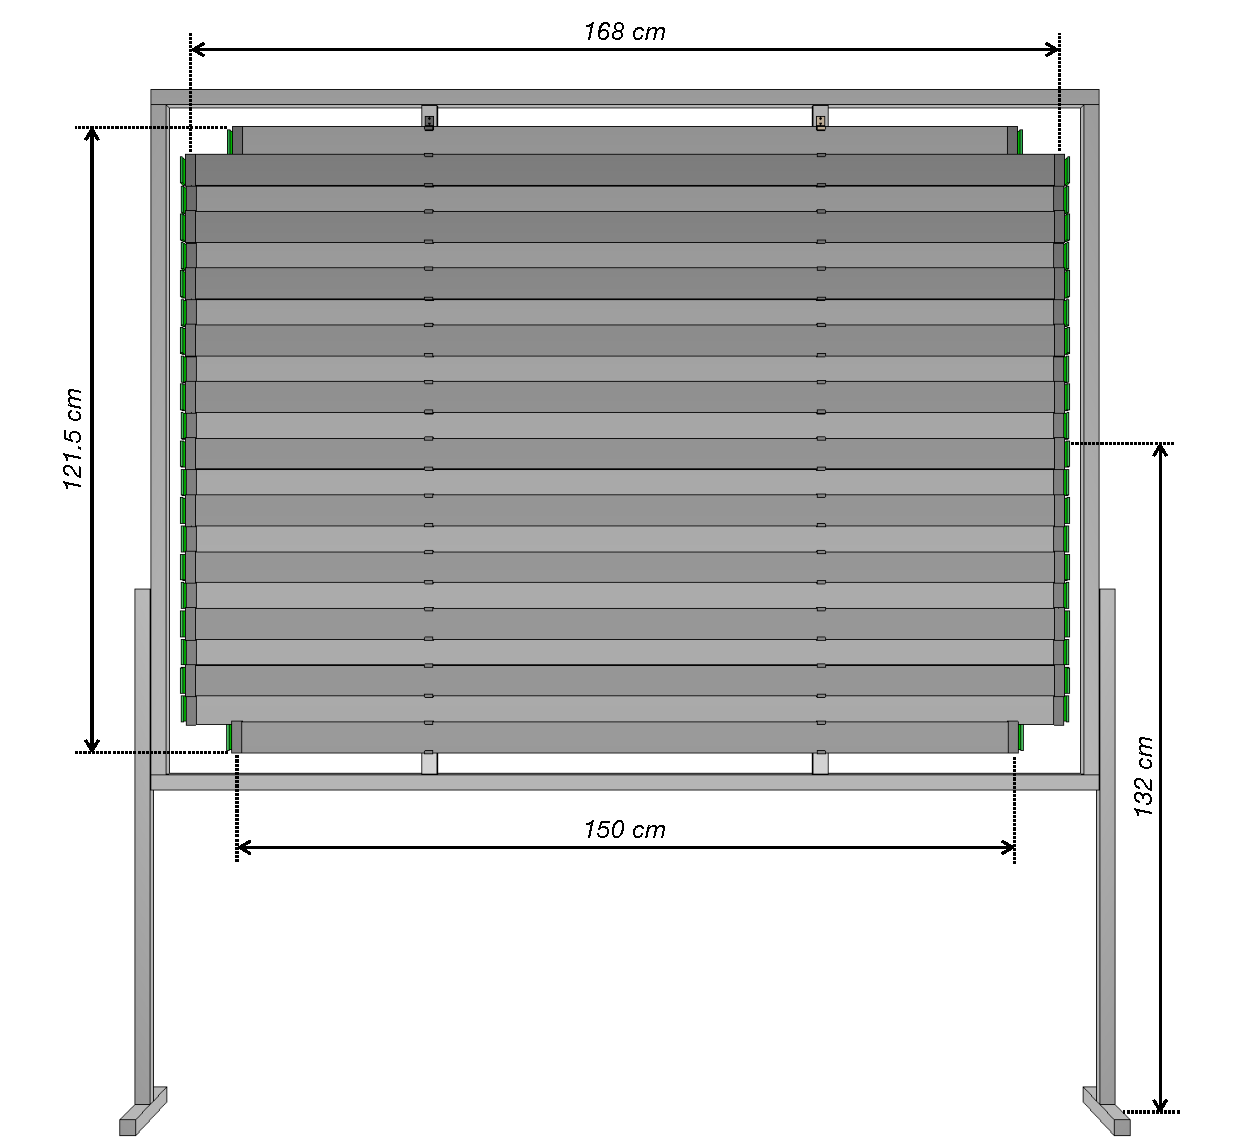
\includegraphics[width=0.52\linewidth]{files/Figures/uToF_sketch.pdf}
  \hfill
  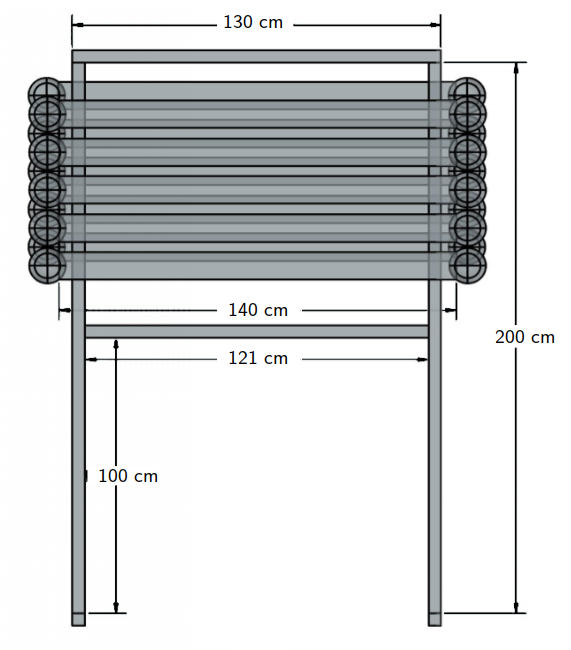
\includegraphics[width=0.47\linewidth]{files/Figures/dstofFront2.png}
  \caption{View of the time of flight panels.
  Left: The $\mathit{S3}$ panel~\cite{S3-proceedings} upstream of the TPC. Right: The $\mathit{S4}$ panel downstream of the TPC.}
  \label{fig:S3sketch}
\end{figure}

The bars are made from EJ-200~\cite{SCIONIX} plastic scintillator, which provides a brightness of 10,000~photons/MeV~deposited.
It also has a suitable optical attenuation length of 4~m and fast timing, with a rise time of 0.9~ns and decay time constant of 2.1~ns.
The scintillation emission spectrum of EJ-200 peaks in the violet region of the visible spectrum (435~nm)~\cite{EJ200}.
The bars were wrapped in an aluminium foil (60\% reflectivity) to increase the collected light.

Arrays of eight $6 \times 6$~mm$^2$ area silicon photomultipliers (SiPMs) S13360-6050PE from Hamamatsu Photonics \cite{Hamamatsu} were coupled to each end of the bar to collect scintillation photons.
The photon detection efficiency at the peak sensitivity wavelength (450~nm) is 40\%~\cite{Hamamatsu}.
The anode signals of the SiPMs are read out, summed and shaped by a dedicated circuit as described in Ref.\,\cite{S3-readout}.
%an 8-channel SiPM anode readout integrated circuit MUSIC-R1. %The construction of the prototype was a joint effort between groups of Geneva and Zurich universities as a part of R\&D for the Timing detector of the SHIP experiment \cite{AK}.

$\mathit{S3}$ uses a 64 channel data acquisition system based on the SAMPIC chip.
A SAMPIC chip is a waveform and time to digital converter (WTDC) 16-channel ASIC which provides a raw time with ultrafast analog memory allowing fine timing extraction as well as other parameters of the pulse~\cite{SAMPIC}.
Each channel contains a discriminator that can trigger itself independently or participate in a more complex combined trigger. 
Three ASIC modules ($16\times3=48$ channels) were connected to the 44 channels of $\mathit{S3}$ and were operated in self-triggering mode.

The trigger conditions are as follows: at least three out of the four $\mathit{S1}$ PMTs must have a signal above a 30~mV threshold.
Additionally, there must be at least one signal in $\mathit{S3}$ above 30~mV.
These $\mathit{S1}$ and $\mathit{S3}$ signals must be coincident within a gate of 70~ns.
A fourth ASIC was used to acquire data from $\mathit{S1}$, the coincidence signal $\mathit{S1} \cap \mathit{S2}$, and the start-of-spill signal from the PS.
%A second level trigger was implemented in firmware and run on the level of the ASICs: the data were only sent to the hard disk of the DAQ computer if there was a coincidence between the $\mathit{S1}$ channels and at least one of the channels in the ASICs used for $\mathit{S3}$.
The mean time of light signals detected at both ends of a single bar provides a time reference with a resolution of about 100~ps, while the difference between the time of the light signals gives the position of the interaction along the bar, with a resolution of 1.6~cm.

Examples of reconstructed $\mathit{S3}$ spatial distributions are shown in Figure~\ref{fig:s3XY_pion}.
Figure~\ref{fig:s3XY_pion}, left, shows the spatial distribution of hits in $\mathit{S3}$ thought to be produced by MIPs when 4 moderator blocks were in the beamline.
Figure~\ref{fig:s3XY_pion}, right, shows the spatial distribution of hits identified in $\mathit{S3}$ as protons when 4 moderator blocks were in the beamline.
The pattern of hits is more diffuse, illustrating the scattering effect of the moderator blocks.
When in this position, the measured horizontal FWHM of the unmoderated beam is 16.8~cm while the vertical FWHM is 11.0~cm.
With 4 moderator blocks in the beamline, the measured horizontal FWHM of the beam is 63.8~cm while the vertical FWHM is 60.0~cm.

\begin{figure}[t]
  \begin{minipage}[t]{0.49\textwidth}
    \centering
    \begin{adjustbox}{max totalsize={\textwidth}{.5\textheight},center}
      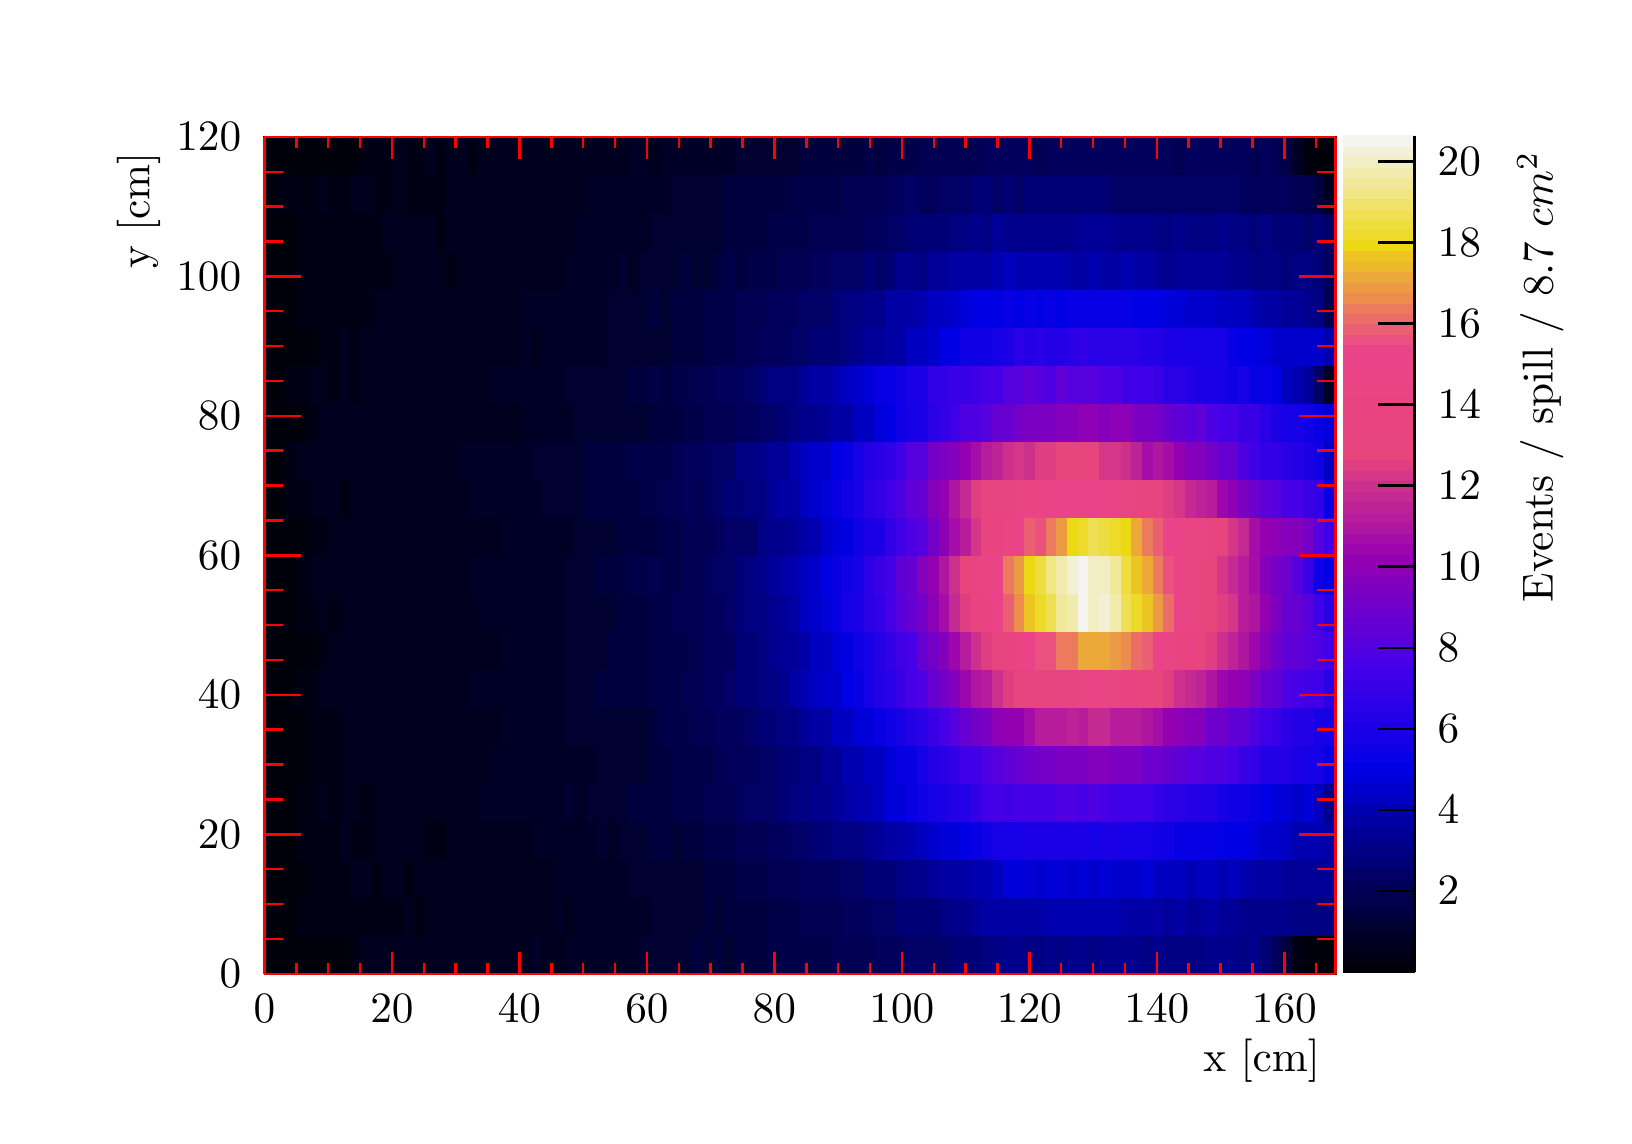
\begin{tikzpicture}
\pgfdeclareplotmark{cross} {
\pgfpathmoveto{\pgfpoint{-0.3\pgfplotmarksize}{\pgfplotmarksize}}
\pgfpathlineto{\pgfpoint{+0.3\pgfplotmarksize}{\pgfplotmarksize}}
\pgfpathlineto{\pgfpoint{+0.3\pgfplotmarksize}{0.3\pgfplotmarksize}}
\pgfpathlineto{\pgfpoint{+1\pgfplotmarksize}{0.3\pgfplotmarksize}}
\pgfpathlineto{\pgfpoint{+1\pgfplotmarksize}{-0.3\pgfplotmarksize}}
\pgfpathlineto{\pgfpoint{+0.3\pgfplotmarksize}{-0.3\pgfplotmarksize}}
\pgfpathlineto{\pgfpoint{+0.3\pgfplotmarksize}{-1.\pgfplotmarksize}}
\pgfpathlineto{\pgfpoint{-0.3\pgfplotmarksize}{-1.\pgfplotmarksize}}
\pgfpathlineto{\pgfpoint{-0.3\pgfplotmarksize}{-0.3\pgfplotmarksize}}
\pgfpathlineto{\pgfpoint{-1.\pgfplotmarksize}{-0.3\pgfplotmarksize}}
\pgfpathlineto{\pgfpoint{-1.\pgfplotmarksize}{0.3\pgfplotmarksize}}
\pgfpathlineto{\pgfpoint{-0.3\pgfplotmarksize}{0.3\pgfplotmarksize}}
\pgfpathclose
\pgfusepathqstroke
}
\pgfdeclareplotmark{cross*} {
\pgfpathmoveto{\pgfpoint{-0.3\pgfplotmarksize}{\pgfplotmarksize}}
\pgfpathlineto{\pgfpoint{+0.3\pgfplotmarksize}{\pgfplotmarksize}}
\pgfpathlineto{\pgfpoint{+0.3\pgfplotmarksize}{0.3\pgfplotmarksize}}
\pgfpathlineto{\pgfpoint{+1\pgfplotmarksize}{0.3\pgfplotmarksize}}
\pgfpathlineto{\pgfpoint{+1\pgfplotmarksize}{-0.3\pgfplotmarksize}}
\pgfpathlineto{\pgfpoint{+0.3\pgfplotmarksize}{-0.3\pgfplotmarksize}}
\pgfpathlineto{\pgfpoint{+0.3\pgfplotmarksize}{-1.\pgfplotmarksize}}
\pgfpathlineto{\pgfpoint{-0.3\pgfplotmarksize}{-1.\pgfplotmarksize}}
\pgfpathlineto{\pgfpoint{-0.3\pgfplotmarksize}{-0.3\pgfplotmarksize}}
\pgfpathlineto{\pgfpoint{-1.\pgfplotmarksize}{-0.3\pgfplotmarksize}}
\pgfpathlineto{\pgfpoint{-1.\pgfplotmarksize}{0.3\pgfplotmarksize}}
\pgfpathlineto{\pgfpoint{-0.3\pgfplotmarksize}{0.3\pgfplotmarksize}}
\pgfpathclose
\pgfusepathqfillstroke
}
\pgfdeclareplotmark{newstar} {
\pgfpathmoveto{\pgfqpoint{0pt}{\pgfplotmarksize}}
\pgfpathlineto{\pgfqpointpolar{44}{0.5\pgfplotmarksize}}
\pgfpathlineto{\pgfqpointpolar{18}{\pgfplotmarksize}}
\pgfpathlineto{\pgfqpointpolar{-20}{0.5\pgfplotmarksize}}
\pgfpathlineto{\pgfqpointpolar{-54}{\pgfplotmarksize}}
\pgfpathlineto{\pgfqpointpolar{-90}{0.5\pgfplotmarksize}}
\pgfpathlineto{\pgfqpointpolar{234}{\pgfplotmarksize}}
\pgfpathlineto{\pgfqpointpolar{198}{0.5\pgfplotmarksize}}
\pgfpathlineto{\pgfqpointpolar{162}{\pgfplotmarksize}}
\pgfpathlineto{\pgfqpointpolar{134}{0.5\pgfplotmarksize}}
\pgfpathclose
\pgfusepathqstroke
}
\pgfdeclareplotmark{newstar*} {
\pgfpathmoveto{\pgfqpoint{0pt}{\pgfplotmarksize}}
\pgfpathlineto{\pgfqpointpolar{44}{0.5\pgfplotmarksize}}
\pgfpathlineto{\pgfqpointpolar{18}{\pgfplotmarksize}}
\pgfpathlineto{\pgfqpointpolar{-20}{0.5\pgfplotmarksize}}
\pgfpathlineto{\pgfqpointpolar{-54}{\pgfplotmarksize}}
\pgfpathlineto{\pgfqpointpolar{-90}{0.5\pgfplotmarksize}}
\pgfpathlineto{\pgfqpointpolar{234}{\pgfplotmarksize}}
\pgfpathlineto{\pgfqpointpolar{198}{0.5\pgfplotmarksize}}
\pgfpathlineto{\pgfqpointpolar{162}{\pgfplotmarksize}}
\pgfpathlineto{\pgfqpointpolar{134}{0.5\pgfplotmarksize}}
\pgfpathclose
\pgfusepathqfillstroke
}
\definecolor{c}{rgb}{1,1,1};
\draw [color=c, fill=c] (0,0) rectangle (20,13.8028);
\draw [color=c, fill=c] (3,1.79437) rectangle (16.6,12.4225);
\definecolor{c}{rgb}{0,0,0};
\draw [c,line width=0.9] (3,1.79437) -- (3,12.4225) -- (16.6,12.4225) -- (16.6,1.79437) -- (3,1.79437);
\definecolor{c}{rgb}{1,1,1};
\draw [color=c, fill=c] (3,1.79437) rectangle (16.6,12.4225);
\definecolor{c}{rgb}{0,0,0};
\draw [c,line width=0.9] (3,1.79437) -- (3,12.4225) -- (16.6,12.4225) -- (16.6,1.79437) -- (3,1.79437);
\definecolor{c}{rgb}{0,0,0.0387097};
\draw [color=c, fill=c] (3,1.79437) rectangle (3.136,2.27746);
\draw [color=c, fill=c] (3.136,1.79437) rectangle (3.272,2.27746);
\draw [color=c, fill=c] (3.272,1.79437) rectangle (3.408,2.27746);
\draw [color=c, fill=c] (3.408,1.79437) rectangle (3.544,2.27746);
\draw [color=c, fill=c] (3.544,1.79437) rectangle (3.68,2.27746);
\draw [color=c, fill=c] (3.68,1.79437) rectangle (3.816,2.27746);
\draw [color=c, fill=c] (3.816,1.79437) rectangle (3.952,2.27746);
\draw [color=c, fill=c] (3.952,1.79437) rectangle (4.088,2.27746);
\definecolor{c}{rgb}{0,0,0.0774194};
\draw [color=c, fill=c] (4.088,1.79437) rectangle (4.224,2.27746);
\definecolor{c}{rgb}{0,0,0.116129};
\draw [color=c, fill=c] (4.224,1.79437) rectangle (4.36,2.27746);
\draw [color=c, fill=c] (4.36,1.79437) rectangle (4.496,2.27746);
\draw [color=c, fill=c] (4.496,1.79437) rectangle (4.632,2.27746);
\draw [color=c, fill=c] (4.632,1.79437) rectangle (4.768,2.27746);
\draw [color=c, fill=c] (4.768,1.79437) rectangle (4.904,2.27746);
\draw [color=c, fill=c] (4.904,1.79437) rectangle (5.04,2.27746);
\draw [color=c, fill=c] (5.04,1.79437) rectangle (5.176,2.27746);
\draw [color=c, fill=c] (5.176,1.79437) rectangle (5.312,2.27746);
\draw [color=c, fill=c] (5.312,1.79437) rectangle (5.448,2.27746);
\draw [color=c, fill=c] (5.448,1.79437) rectangle (5.584,2.27746);
\draw [color=c, fill=c] (5.584,1.79437) rectangle (5.72,2.27746);
\draw [color=c, fill=c] (5.72,1.79437) rectangle (5.856,2.27746);
\draw [color=c, fill=c] (5.856,1.79437) rectangle (5.992,2.27746);
\draw [color=c, fill=c] (5.992,1.79437) rectangle (6.128,2.27746);
\draw [color=c, fill=c] (6.128,1.79437) rectangle (6.264,2.27746);
\draw [color=c, fill=c] (6.264,1.79437) rectangle (6.4,2.27746);
\definecolor{c}{rgb}{0,0,0.154839};
\draw [color=c, fill=c] (6.4,1.79437) rectangle (6.536,2.27746);
\definecolor{c}{rgb}{0,0,0.116129};
\draw [color=c, fill=c] (6.536,1.79437) rectangle (6.672,2.27746);
\draw [color=c, fill=c] (6.672,1.79437) rectangle (6.808,2.27746);
\definecolor{c}{rgb}{0,0,0.154839};
\draw [color=c, fill=c] (6.808,1.79437) rectangle (6.944,2.27746);
\draw [color=c, fill=c] (6.944,1.79437) rectangle (7.08,2.27746);
\draw [color=c, fill=c] (7.08,1.79437) rectangle (7.216,2.27746);
\draw [color=c, fill=c] (7.216,1.79437) rectangle (7.352,2.27746);
\draw [color=c, fill=c] (7.352,1.79437) rectangle (7.488,2.27746);
\draw [color=c, fill=c] (7.488,1.79437) rectangle (7.624,2.27746);
\draw [color=c, fill=c] (7.624,1.79437) rectangle (7.76,2.27746);
\definecolor{c}{rgb}{0,0,0.193548};
\draw [color=c, fill=c] (7.76,1.79437) rectangle (7.896,2.27746);
\draw [color=c, fill=c] (7.896,1.79437) rectangle (8.032,2.27746);
\draw [color=c, fill=c] (8.032,1.79437) rectangle (8.168,2.27746);
\draw [color=c, fill=c] (8.168,1.79437) rectangle (8.304,2.27746);
\draw [color=c, fill=c] (8.304,1.79437) rectangle (8.44,2.27746);
\definecolor{c}{rgb}{0,0,0.245161};
\draw [color=c, fill=c] (8.44,1.79437) rectangle (8.576,2.27746);
\definecolor{c}{rgb}{0,0,0.193548};
\draw [color=c, fill=c] (8.576,1.79437) rectangle (8.712,2.27746);
\definecolor{c}{rgb}{0,0,0.245161};
\draw [color=c, fill=c] (8.712,1.79437) rectangle (8.848,2.27746);
\definecolor{c}{rgb}{0,0,0.193548};
\draw [color=c, fill=c] (8.848,1.79437) rectangle (8.984,2.27746);
\definecolor{c}{rgb}{0,0,0.245161};
\draw [color=c, fill=c] (8.984,1.79437) rectangle (9.12,2.27746);
\draw [color=c, fill=c] (9.12,1.79437) rectangle (9.256,2.27746);
\draw [color=c, fill=c] (9.256,1.79437) rectangle (9.392,2.27746);
\definecolor{c}{rgb}{0,0,0.283871};
\draw [color=c, fill=c] (9.392,1.79437) rectangle (9.528,2.27746);
\draw [color=c, fill=c] (9.528,1.79437) rectangle (9.664,2.27746);
\draw [color=c, fill=c] (9.664,1.79437) rectangle (9.8,2.27746);
\draw [color=c, fill=c] (9.8,1.79437) rectangle (9.936,2.27746);
\draw [color=c, fill=c] (9.936,1.79437) rectangle (10.072,2.27746);
\draw [color=c, fill=c] (10.072,1.79437) rectangle (10.208,2.27746);
\definecolor{c}{rgb}{0,0,0.322581};
\draw [color=c, fill=c] (10.208,1.79437) rectangle (10.344,2.27746);
\draw [color=c, fill=c] (10.344,1.79437) rectangle (10.48,2.27746);
\draw [color=c, fill=c] (10.48,1.79437) rectangle (10.616,2.27746);
\draw [color=c, fill=c] (10.616,1.79437) rectangle (10.752,2.27746);
\definecolor{c}{rgb}{0,0,0.36129};
\draw [color=c, fill=c] (10.752,1.79437) rectangle (10.888,2.27746);
\draw [color=c, fill=c] (10.888,1.79437) rectangle (11.024,2.27746);
\draw [color=c, fill=c] (11.024,1.79437) rectangle (11.16,2.27746);
\definecolor{c}{rgb}{0,0,0.4};
\draw [color=c, fill=c] (11.16,1.79437) rectangle (11.296,2.27746);
\draw [color=c, fill=c] (11.296,1.79437) rectangle (11.432,2.27746);
\draw [color=c, fill=c] (11.432,1.79437) rectangle (11.568,2.27746);
\draw [color=c, fill=c] (11.568,1.79437) rectangle (11.704,2.27746);
\definecolor{c}{rgb}{0,0,0.461765};
\draw [color=c, fill=c] (11.704,1.79437) rectangle (11.84,2.27746);
\draw [color=c, fill=c] (11.84,1.79437) rectangle (11.976,2.27746);
\draw [color=c, fill=c] (11.976,1.79437) rectangle (12.112,2.27746);
\definecolor{c}{rgb}{0,0,0.508088};
\draw [color=c, fill=c] (12.112,1.79437) rectangle (12.248,2.27746);
\draw [color=c, fill=c] (12.248,1.79437) rectangle (12.384,2.27746);
\definecolor{c}{rgb}{0,0,0.554412};
\draw [color=c, fill=c] (12.384,1.79437) rectangle (12.52,2.27746);
\draw [color=c, fill=c] (12.52,1.79437) rectangle (12.656,2.27746);
\definecolor{c}{rgb}{0,0,0.508088};
\draw [color=c, fill=c] (12.656,1.79437) rectangle (12.792,2.27746);
\draw [color=c, fill=c] (12.792,1.79437) rectangle (12.928,2.27746);
\definecolor{c}{rgb}{0,0,0.554412};
\draw [color=c, fill=c] (12.928,1.79437) rectangle (13.064,2.27746);
\definecolor{c}{rgb}{0,0,0.508088};
\draw [color=c, fill=c] (13.064,1.79437) rectangle (13.2,2.27746);
\definecolor{c}{rgb}{0,0,0.554412};
\draw [color=c, fill=c] (13.2,1.79437) rectangle (13.336,2.27746);
\draw [color=c, fill=c] (13.336,1.79437) rectangle (13.472,2.27746);
\definecolor{c}{rgb}{0,0,0.508088};
\draw [color=c, fill=c] (13.472,1.79437) rectangle (13.608,2.27746);
\definecolor{c}{rgb}{0,0,0.554412};
\draw [color=c, fill=c] (13.608,1.79437) rectangle (13.744,2.27746);
\draw [color=c, fill=c] (13.744,1.79437) rectangle (13.88,2.27746);
\draw [color=c, fill=c] (13.88,1.79437) rectangle (14.016,2.27746);
\draw [color=c, fill=c] (14.016,1.79437) rectangle (14.152,2.27746);
\definecolor{c}{rgb}{0,0,0.508088};
\draw [color=c, fill=c] (14.152,1.79437) rectangle (14.288,2.27746);
\definecolor{c}{rgb}{0,0,0.554412};
\draw [color=c, fill=c] (14.288,1.79437) rectangle (14.424,2.27746);
\definecolor{c}{rgb}{0,0,0.508088};
\draw [color=c, fill=c] (14.424,1.79437) rectangle (14.56,2.27746);
\draw [color=c, fill=c] (14.56,1.79437) rectangle (14.696,2.27746);
\draw [color=c, fill=c] (14.696,1.79437) rectangle (14.832,2.27746);
\draw [color=c, fill=c] (14.832,1.79437) rectangle (14.968,2.27746);
\definecolor{c}{rgb}{0,0,0.554412};
\draw [color=c, fill=c] (14.968,1.79437) rectangle (15.104,2.27746);
\draw [color=c, fill=c] (15.104,1.79437) rectangle (15.24,2.27746);
\draw [color=c, fill=c] (15.24,1.79437) rectangle (15.376,2.27746);
\definecolor{c}{rgb}{0,0,0.508088};
\draw [color=c, fill=c] (15.376,1.79437) rectangle (15.512,2.27746);
\definecolor{c}{rgb}{0,0,0.554412};
\draw [color=c, fill=c] (15.512,1.79437) rectangle (15.648,2.27746);
\definecolor{c}{rgb}{0,0,0.461765};
\draw [color=c, fill=c] (15.648,1.79437) rectangle (15.784,2.27746);
\definecolor{c}{rgb}{0,0,0.36129};
\draw [color=c, fill=c] (15.784,1.79437) rectangle (15.92,2.27746);
\definecolor{c}{rgb}{0,0,0.245161};
\draw [color=c, fill=c] (15.92,1.79437) rectangle (16.056,2.27746);
\definecolor{c}{rgb}{0,0,0.0774194};
\draw [color=c, fill=c] (16.056,1.79437) rectangle (16.192,2.27746);
\definecolor{c}{rgb}{0,0,0.0387097};
\draw [color=c, fill=c] (16.192,1.79437) rectangle (16.328,2.27746);
\draw [color=c, fill=c] (16.328,1.79437) rectangle (16.464,2.27746);
\draw [color=c, fill=c] (16.464,1.79437) rectangle (16.6,2.27746);
\draw [color=c, fill=c] (3,2.27746) rectangle (3.136,2.76056);
\draw [color=c, fill=c] (3.136,2.27746) rectangle (3.272,2.76056);
\draw [color=c, fill=c] (3.272,2.27746) rectangle (3.408,2.76056);
\definecolor{c}{rgb}{0,0,0.0774194};
\draw [color=c, fill=c] (3.408,2.27746) rectangle (3.544,2.76056);
\draw [color=c, fill=c] (3.544,2.27746) rectangle (3.68,2.76056);
\draw [color=c, fill=c] (3.68,2.27746) rectangle (3.816,2.76056);
\draw [color=c, fill=c] (3.816,2.27746) rectangle (3.952,2.76056);
\draw [color=c, fill=c] (3.952,2.27746) rectangle (4.088,2.76056);
\draw [color=c, fill=c] (4.088,2.27746) rectangle (4.224,2.76056);
\draw [color=c, fill=c] (4.224,2.27746) rectangle (4.36,2.76056);
\draw [color=c, fill=c] (4.36,2.27746) rectangle (4.496,2.76056);
\draw [color=c, fill=c] (4.496,2.27746) rectangle (4.632,2.76056);
\draw [color=c, fill=c] (4.632,2.27746) rectangle (4.768,2.76056);
\definecolor{c}{rgb}{0,0,0.116129};
\draw [color=c, fill=c] (4.768,2.27746) rectangle (4.904,2.76056);
\definecolor{c}{rgb}{0,0,0.0774194};
\draw [color=c, fill=c] (4.904,2.27746) rectangle (5.04,2.76056);
\definecolor{c}{rgb}{0,0,0.116129};
\draw [color=c, fill=c] (5.04,2.27746) rectangle (5.176,2.76056);
\draw [color=c, fill=c] (5.176,2.27746) rectangle (5.312,2.76056);
\draw [color=c, fill=c] (5.312,2.27746) rectangle (5.448,2.76056);
\draw [color=c, fill=c] (5.448,2.27746) rectangle (5.584,2.76056);
\draw [color=c, fill=c] (5.584,2.27746) rectangle (5.72,2.76056);
\draw [color=c, fill=c] (5.72,2.27746) rectangle (5.856,2.76056);
\draw [color=c, fill=c] (5.856,2.27746) rectangle (5.992,2.76056);
\draw [color=c, fill=c] (5.992,2.27746) rectangle (6.128,2.76056);
\draw [color=c, fill=c] (6.128,2.27746) rectangle (6.264,2.76056);
\draw [color=c, fill=c] (6.264,2.27746) rectangle (6.4,2.76056);
\draw [color=c, fill=c] (6.4,2.27746) rectangle (6.536,2.76056);
\draw [color=c, fill=c] (6.536,2.27746) rectangle (6.672,2.76056);
\definecolor{c}{rgb}{0,0,0.154839};
\draw [color=c, fill=c] (6.672,2.27746) rectangle (6.808,2.76056);
\definecolor{c}{rgb}{0,0,0.116129};
\draw [color=c, fill=c] (6.808,2.27746) rectangle (6.944,2.76056);
\definecolor{c}{rgb}{0,0,0.154839};
\draw [color=c, fill=c] (6.944,2.27746) rectangle (7.08,2.76056);
\draw [color=c, fill=c] (7.08,2.27746) rectangle (7.216,2.76056);
\draw [color=c, fill=c] (7.216,2.27746) rectangle (7.352,2.76056);
\draw [color=c, fill=c] (7.352,2.27746) rectangle (7.488,2.76056);
\draw [color=c, fill=c] (7.488,2.27746) rectangle (7.624,2.76056);
\draw [color=c, fill=c] (7.624,2.27746) rectangle (7.76,2.76056);
\draw [color=c, fill=c] (7.76,2.27746) rectangle (7.896,2.76056);
\definecolor{c}{rgb}{0,0,0.193548};
\draw [color=c, fill=c] (7.896,2.27746) rectangle (8.032,2.76056);
\draw [color=c, fill=c] (8.032,2.27746) rectangle (8.168,2.76056);
\draw [color=c, fill=c] (8.168,2.27746) rectangle (8.304,2.76056);
\draw [color=c, fill=c] (8.304,2.27746) rectangle (8.44,2.76056);
\draw [color=c, fill=c] (8.44,2.27746) rectangle (8.576,2.76056);
\definecolor{c}{rgb}{0,0,0.245161};
\draw [color=c, fill=c] (8.576,2.27746) rectangle (8.712,2.76056);
\definecolor{c}{rgb}{0,0,0.193548};
\draw [color=c, fill=c] (8.712,2.27746) rectangle (8.848,2.76056);
\definecolor{c}{rgb}{0,0,0.245161};
\draw [color=c, fill=c] (8.848,2.27746) rectangle (8.984,2.76056);
\draw [color=c, fill=c] (8.984,2.27746) rectangle (9.12,2.76056);
\draw [color=c, fill=c] (9.12,2.27746) rectangle (9.256,2.76056);
\draw [color=c, fill=c] (9.256,2.27746) rectangle (9.392,2.76056);
\definecolor{c}{rgb}{0,0,0.283871};
\draw [color=c, fill=c] (9.392,2.27746) rectangle (9.528,2.76056);
\draw [color=c, fill=c] (9.528,2.27746) rectangle (9.664,2.76056);
\draw [color=c, fill=c] (9.664,2.27746) rectangle (9.8,2.76056);
\definecolor{c}{rgb}{0,0,0.322581};
\draw [color=c, fill=c] (9.8,2.27746) rectangle (9.936,2.76056);
\draw [color=c, fill=c] (9.936,2.27746) rectangle (10.072,2.76056);
\draw [color=c, fill=c] (10.072,2.27746) rectangle (10.208,2.76056);
\draw [color=c, fill=c] (10.208,2.27746) rectangle (10.344,2.76056);
\definecolor{c}{rgb}{0,0,0.36129};
\draw [color=c, fill=c] (10.344,2.27746) rectangle (10.48,2.76056);
\draw [color=c, fill=c] (10.48,2.27746) rectangle (10.616,2.76056);
\draw [color=c, fill=c] (10.616,2.27746) rectangle (10.752,2.76056);
\definecolor{c}{rgb}{0,0,0.4};
\draw [color=c, fill=c] (10.752,2.27746) rectangle (10.888,2.76056);
\draw [color=c, fill=c] (10.888,2.27746) rectangle (11.024,2.76056);
\definecolor{c}{rgb}{0,0,0.461765};
\draw [color=c, fill=c] (11.024,2.27746) rectangle (11.16,2.76056);
\draw [color=c, fill=c] (11.16,2.27746) rectangle (11.296,2.76056);
\draw [color=c, fill=c] (11.296,2.27746) rectangle (11.432,2.76056);
\draw [color=c, fill=c] (11.432,2.27746) rectangle (11.568,2.76056);
\definecolor{c}{rgb}{0,0,0.508088};
\draw [color=c, fill=c] (11.568,2.27746) rectangle (11.704,2.76056);
\definecolor{c}{rgb}{0,0,0.554412};
\draw [color=c, fill=c] (11.704,2.27746) rectangle (11.84,2.76056);
\draw [color=c, fill=c] (11.84,2.27746) rectangle (11.976,2.76056);
\definecolor{c}{rgb}{0,0,0.600735};
\draw [color=c, fill=c] (11.976,2.27746) rectangle (12.112,2.76056);
\definecolor{c}{rgb}{0,0,0.647059};
\draw [color=c, fill=c] (12.112,2.27746) rectangle (12.248,2.76056);
\draw [color=c, fill=c] (12.248,2.27746) rectangle (12.384,2.76056);
\draw [color=c, fill=c] (12.384,2.27746) rectangle (12.52,2.76056);
\draw [color=c, fill=c] (12.52,2.27746) rectangle (12.656,2.76056);
\draw [color=c, fill=c] (12.656,2.27746) rectangle (12.792,2.76056);
\draw [color=c, fill=c] (12.792,2.27746) rectangle (12.928,2.76056);
\definecolor{c}{rgb}{0,0,0.693382};
\draw [color=c, fill=c] (12.928,2.27746) rectangle (13.064,2.76056);
\draw [color=c, fill=c] (13.064,2.27746) rectangle (13.2,2.76056);
\draw [color=c, fill=c] (13.2,2.27746) rectangle (13.336,2.76056);
\draw [color=c, fill=c] (13.336,2.27746) rectangle (13.472,2.76056);
\draw [color=c, fill=c] (13.472,2.27746) rectangle (13.608,2.76056);
\draw [color=c, fill=c] (13.608,2.27746) rectangle (13.744,2.76056);
\draw [color=c, fill=c] (13.744,2.27746) rectangle (13.88,2.76056);
\definecolor{c}{rgb}{0,0,0.647059};
\draw [color=c, fill=c] (13.88,2.27746) rectangle (14.016,2.76056);
\draw [color=c, fill=c] (14.016,2.27746) rectangle (14.152,2.76056);
\draw [color=c, fill=c] (14.152,2.27746) rectangle (14.288,2.76056);
\draw [color=c, fill=c] (14.288,2.27746) rectangle (14.424,2.76056);
\definecolor{c}{rgb}{0,0,0.600735};
\draw [color=c, fill=c] (14.424,2.27746) rectangle (14.56,2.76056);
\definecolor{c}{rgb}{0,0,0.647059};
\draw [color=c, fill=c] (14.56,2.27746) rectangle (14.696,2.76056);
\definecolor{c}{rgb}{0,0,0.600735};
\draw [color=c, fill=c] (14.696,2.27746) rectangle (14.832,2.76056);
\draw [color=c, fill=c] (14.832,2.27746) rectangle (14.968,2.76056);
\definecolor{c}{rgb}{0,0,0.647059};
\draw [color=c, fill=c] (14.968,2.27746) rectangle (15.104,2.76056);
\definecolor{c}{rgb}{0,0,0.600735};
\draw [color=c, fill=c] (15.104,2.27746) rectangle (15.24,2.76056);
\draw [color=c, fill=c] (15.24,2.27746) rectangle (15.376,2.76056);
\definecolor{c}{rgb}{0,0,0.554412};
\draw [color=c, fill=c] (15.376,2.27746) rectangle (15.512,2.76056);
\draw [color=c, fill=c] (15.512,2.27746) rectangle (15.648,2.76056);
\draw [color=c, fill=c] (15.648,2.27746) rectangle (15.784,2.76056);
\draw [color=c, fill=c] (15.784,2.27746) rectangle (15.92,2.76056);
\draw [color=c, fill=c] (15.92,2.27746) rectangle (16.056,2.76056);
\definecolor{c}{rgb}{0,0,0.508088};
\draw [color=c, fill=c] (16.056,2.27746) rectangle (16.192,2.76056);
\draw [color=c, fill=c] (16.192,2.27746) rectangle (16.328,2.76056);
\draw [color=c, fill=c] (16.328,2.27746) rectangle (16.464,2.76056);
\draw [color=c, fill=c] (16.464,2.27746) rectangle (16.6,2.76056);
\definecolor{c}{rgb}{0,0,0.0387097};
\draw [color=c, fill=c] (3,2.76056) rectangle (3.136,3.24366);
\draw [color=c, fill=c] (3.136,2.76056) rectangle (3.272,3.24366);
\draw [color=c, fill=c] (3.272,2.76056) rectangle (3.408,3.24366);
\draw [color=c, fill=c] (3.408,2.76056) rectangle (3.544,3.24366);
\definecolor{c}{rgb}{0,0,0.0774194};
\draw [color=c, fill=c] (3.544,2.76056) rectangle (3.68,3.24366);
\draw [color=c, fill=c] (3.68,2.76056) rectangle (3.816,3.24366);
\draw [color=c, fill=c] (3.816,2.76056) rectangle (3.952,3.24366);
\draw [color=c, fill=c] (3.952,2.76056) rectangle (4.088,3.24366);
\definecolor{c}{rgb}{0,0,0.116129};
\draw [color=c, fill=c] (4.088,2.76056) rectangle (4.224,3.24366);
\draw [color=c, fill=c] (4.224,2.76056) rectangle (4.36,3.24366);
\definecolor{c}{rgb}{0,0,0.0774194};
\draw [color=c, fill=c] (4.36,2.76056) rectangle (4.496,3.24366);
\definecolor{c}{rgb}{0,0,0.116129};
\draw [color=c, fill=c] (4.496,2.76056) rectangle (4.632,3.24366);
\draw [color=c, fill=c] (4.632,2.76056) rectangle (4.768,3.24366);
\definecolor{c}{rgb}{0,0,0.0774194};
\draw [color=c, fill=c] (4.768,2.76056) rectangle (4.904,3.24366);
\definecolor{c}{rgb}{0,0,0.116129};
\draw [color=c, fill=c] (4.904,2.76056) rectangle (5.04,3.24366);
\draw [color=c, fill=c] (5.04,2.76056) rectangle (5.176,3.24366);
\draw [color=c, fill=c] (5.176,2.76056) rectangle (5.312,3.24366);
\draw [color=c, fill=c] (5.312,2.76056) rectangle (5.448,3.24366);
\draw [color=c, fill=c] (5.448,2.76056) rectangle (5.584,3.24366);
\draw [color=c, fill=c] (5.584,2.76056) rectangle (5.72,3.24366);
\draw [color=c, fill=c] (5.72,2.76056) rectangle (5.856,3.24366);
\draw [color=c, fill=c] (5.856,2.76056) rectangle (5.992,3.24366);
\draw [color=c, fill=c] (5.992,2.76056) rectangle (6.128,3.24366);
\draw [color=c, fill=c] (6.128,2.76056) rectangle (6.264,3.24366);
\draw [color=c, fill=c] (6.264,2.76056) rectangle (6.4,3.24366);
\draw [color=c, fill=c] (6.4,2.76056) rectangle (6.536,3.24366);
\draw [color=c, fill=c] (6.536,2.76056) rectangle (6.672,3.24366);
\definecolor{c}{rgb}{0,0,0.154839};
\draw [color=c, fill=c] (6.672,2.76056) rectangle (6.808,3.24366);
\draw [color=c, fill=c] (6.808,2.76056) rectangle (6.944,3.24366);
\draw [color=c, fill=c] (6.944,2.76056) rectangle (7.08,3.24366);
\draw [color=c, fill=c] (7.08,2.76056) rectangle (7.216,3.24366);
\draw [color=c, fill=c] (7.216,2.76056) rectangle (7.352,3.24366);
\draw [color=c, fill=c] (7.352,2.76056) rectangle (7.488,3.24366);
\draw [color=c, fill=c] (7.488,2.76056) rectangle (7.624,3.24366);
\definecolor{c}{rgb}{0,0,0.193548};
\draw [color=c, fill=c] (7.624,2.76056) rectangle (7.76,3.24366);
\draw [color=c, fill=c] (7.76,2.76056) rectangle (7.896,3.24366);
\draw [color=c, fill=c] (7.896,2.76056) rectangle (8.032,3.24366);
\draw [color=c, fill=c] (8.032,2.76056) rectangle (8.168,3.24366);
\draw [color=c, fill=c] (8.168,2.76056) rectangle (8.304,3.24366);
\draw [color=c, fill=c] (8.304,2.76056) rectangle (8.44,3.24366);
\draw [color=c, fill=c] (8.44,2.76056) rectangle (8.576,3.24366);
\definecolor{c}{rgb}{0,0,0.245161};
\draw [color=c, fill=c] (8.576,2.76056) rectangle (8.712,3.24366);
\draw [color=c, fill=c] (8.712,2.76056) rectangle (8.848,3.24366);
\draw [color=c, fill=c] (8.848,2.76056) rectangle (8.984,3.24366);
\definecolor{c}{rgb}{0,0,0.283871};
\draw [color=c, fill=c] (8.984,2.76056) rectangle (9.12,3.24366);
\draw [color=c, fill=c] (9.12,2.76056) rectangle (9.256,3.24366);
\draw [color=c, fill=c] (9.256,2.76056) rectangle (9.392,3.24366);
\definecolor{c}{rgb}{0,0,0.322581};
\draw [color=c, fill=c] (9.392,2.76056) rectangle (9.528,3.24366);
\draw [color=c, fill=c] (9.528,2.76056) rectangle (9.664,3.24366);
\draw [color=c, fill=c] (9.664,2.76056) rectangle (9.8,3.24366);
\definecolor{c}{rgb}{0,0,0.36129};
\draw [color=c, fill=c] (9.8,2.76056) rectangle (9.936,3.24366);
\draw [color=c, fill=c] (9.936,2.76056) rectangle (10.072,3.24366);
\draw [color=c, fill=c] (10.072,2.76056) rectangle (10.208,3.24366);
\draw [color=c, fill=c] (10.208,2.76056) rectangle (10.344,3.24366);
\definecolor{c}{rgb}{0,0,0.4};
\draw [color=c, fill=c] (10.344,2.76056) rectangle (10.48,3.24366);
\draw [color=c, fill=c] (10.48,2.76056) rectangle (10.616,3.24366);
\definecolor{c}{rgb}{0,0,0.461765};
\draw [color=c, fill=c] (10.616,2.76056) rectangle (10.752,3.24366);
\draw [color=c, fill=c] (10.752,2.76056) rectangle (10.888,3.24366);
\draw [color=c, fill=c] (10.888,2.76056) rectangle (11.024,3.24366);
\definecolor{c}{rgb}{0,0,0.508088};
\draw [color=c, fill=c] (11.024,2.76056) rectangle (11.16,3.24366);
\definecolor{c}{rgb}{0,0,0.554412};
\draw [color=c, fill=c] (11.16,2.76056) rectangle (11.296,3.24366);
\draw [color=c, fill=c] (11.296,2.76056) rectangle (11.432,3.24366);
\definecolor{c}{rgb}{0,0,0.600735};
\draw [color=c, fill=c] (11.432,2.76056) rectangle (11.568,3.24366);
\definecolor{c}{rgb}{0,0,0.647059};
\draw [color=c, fill=c] (11.568,2.76056) rectangle (11.704,3.24366);
\draw [color=c, fill=c] (11.704,2.76056) rectangle (11.84,3.24366);
\draw [color=c, fill=c] (11.84,2.76056) rectangle (11.976,3.24366);
\definecolor{c}{rgb}{0,0,0.693382};
\draw [color=c, fill=c] (11.976,2.76056) rectangle (12.112,3.24366);
\draw [color=c, fill=c] (12.112,2.76056) rectangle (12.248,3.24366);
\definecolor{c}{rgb}{0,0,0.755147};
\draw [color=c, fill=c] (12.248,2.76056) rectangle (12.384,3.24366);
\definecolor{c}{rgb}{0,0,0.847794};
\draw [color=c, fill=c] (12.384,2.76056) rectangle (12.52,3.24366);
\draw [color=c, fill=c] (12.52,2.76056) rectangle (12.656,3.24366);
\draw [color=c, fill=c] (12.656,2.76056) rectangle (12.792,3.24366);
\definecolor{c}{rgb}{0,0,0.801471};
\draw [color=c, fill=c] (12.792,2.76056) rectangle (12.928,3.24366);
\definecolor{c}{rgb}{0,0,0.847794};
\draw [color=c, fill=c] (12.928,2.76056) rectangle (13.064,3.24366);
\draw [color=c, fill=c] (13.064,2.76056) rectangle (13.2,3.24366);
\definecolor{c}{rgb}{0,0,0.801471};
\draw [color=c, fill=c] (13.2,2.76056) rectangle (13.336,3.24366);
\definecolor{c}{rgb}{0,0,0.847794};
\draw [color=c, fill=c] (13.336,2.76056) rectangle (13.472,3.24366);
\definecolor{c}{rgb}{0,0,0.801471};
\draw [color=c, fill=c] (13.472,2.76056) rectangle (13.608,3.24366);
\definecolor{c}{rgb}{0,0,0.847794};
\draw [color=c, fill=c] (13.608,2.76056) rectangle (13.744,3.24366);
\definecolor{c}{rgb}{0,0,0.801471};
\draw [color=c, fill=c] (13.744,2.76056) rectangle (13.88,3.24366);
\draw [color=c, fill=c] (13.88,2.76056) rectangle (14.016,3.24366);
\draw [color=c, fill=c] (14.016,2.76056) rectangle (14.152,3.24366);
\definecolor{c}{rgb}{0,0,0.847794};
\draw [color=c, fill=c] (14.152,2.76056) rectangle (14.288,3.24366);
\definecolor{c}{rgb}{0,0,0.755147};
\draw [color=c, fill=c] (14.288,2.76056) rectangle (14.424,3.24366);
\draw [color=c, fill=c] (14.424,2.76056) rectangle (14.56,3.24366);
\draw [color=c, fill=c] (14.56,2.76056) rectangle (14.696,3.24366);
\definecolor{c}{rgb}{0,0,0.693382};
\draw [color=c, fill=c] (14.696,2.76056) rectangle (14.832,3.24366);
\definecolor{c}{rgb}{0,0,0.755147};
\draw [color=c, fill=c] (14.832,2.76056) rectangle (14.968,3.24366);
\draw [color=c, fill=c] (14.968,2.76056) rectangle (15.104,3.24366);
\definecolor{c}{rgb}{0,0,0.693382};
\draw [color=c, fill=c] (15.104,2.76056) rectangle (15.24,3.24366);
\definecolor{c}{rgb}{0,0,0.755147};
\draw [color=c, fill=c] (15.24,2.76056) rectangle (15.376,3.24366);
\definecolor{c}{rgb}{0,0,0.693382};
\draw [color=c, fill=c] (15.376,2.76056) rectangle (15.512,3.24366);
\definecolor{c}{rgb}{0,0,0.647059};
\draw [color=c, fill=c] (15.512,2.76056) rectangle (15.648,3.24366);
\draw [color=c, fill=c] (15.648,2.76056) rectangle (15.784,3.24366);
\draw [color=c, fill=c] (15.784,2.76056) rectangle (15.92,3.24366);
\definecolor{c}{rgb}{0,0,0.600735};
\draw [color=c, fill=c] (15.92,2.76056) rectangle (16.056,3.24366);
\draw [color=c, fill=c] (16.056,2.76056) rectangle (16.192,3.24366);
\draw [color=c, fill=c] (16.192,2.76056) rectangle (16.328,3.24366);
\draw [color=c, fill=c] (16.328,2.76056) rectangle (16.464,3.24366);
\draw [color=c, fill=c] (16.464,2.76056) rectangle (16.6,3.24366);
\definecolor{c}{rgb}{0,0,0.0387097};
\draw [color=c, fill=c] (3,3.24366) rectangle (3.136,3.72676);
\draw [color=c, fill=c] (3.136,3.24366) rectangle (3.272,3.72676);
\draw [color=c, fill=c] (3.272,3.24366) rectangle (3.408,3.72676);
\definecolor{c}{rgb}{0,0,0.0774194};
\draw [color=c, fill=c] (3.408,3.24366) rectangle (3.544,3.72676);
\draw [color=c, fill=c] (3.544,3.24366) rectangle (3.68,3.72676);
\draw [color=c, fill=c] (3.68,3.24366) rectangle (3.816,3.72676);
\draw [color=c, fill=c] (3.816,3.24366) rectangle (3.952,3.72676);
\definecolor{c}{rgb}{0,0,0.116129};
\draw [color=c, fill=c] (3.952,3.24366) rectangle (4.088,3.72676);
\definecolor{c}{rgb}{0,0,0.0774194};
\draw [color=c, fill=c] (4.088,3.24366) rectangle (4.224,3.72676);
\draw [color=c, fill=c] (4.224,3.24366) rectangle (4.36,3.72676);
\definecolor{c}{rgb}{0,0,0.116129};
\draw [color=c, fill=c] (4.36,3.24366) rectangle (4.496,3.72676);
\draw [color=c, fill=c] (4.496,3.24366) rectangle (4.632,3.72676);
\draw [color=c, fill=c] (4.632,3.24366) rectangle (4.768,3.72676);
\draw [color=c, fill=c] (4.768,3.24366) rectangle (4.904,3.72676);
\draw [color=c, fill=c] (4.904,3.24366) rectangle (5.04,3.72676);
\definecolor{c}{rgb}{0,0,0.0774194};
\draw [color=c, fill=c] (5.04,3.24366) rectangle (5.176,3.72676);
\draw [color=c, fill=c] (5.176,3.24366) rectangle (5.312,3.72676);
\definecolor{c}{rgb}{0,0,0.116129};
\draw [color=c, fill=c] (5.312,3.24366) rectangle (5.448,3.72676);
\draw [color=c, fill=c] (5.448,3.24366) rectangle (5.584,3.72676);
\draw [color=c, fill=c] (5.584,3.24366) rectangle (5.72,3.72676);
\draw [color=c, fill=c] (5.72,3.24366) rectangle (5.856,3.72676);
\draw [color=c, fill=c] (5.856,3.24366) rectangle (5.992,3.72676);
\draw [color=c, fill=c] (5.992,3.24366) rectangle (6.128,3.72676);
\draw [color=c, fill=c] (6.128,3.24366) rectangle (6.264,3.72676);
\draw [color=c, fill=c] (6.264,3.24366) rectangle (6.4,3.72676);
\definecolor{c}{rgb}{0,0,0.154839};
\draw [color=c, fill=c] (6.4,3.24366) rectangle (6.536,3.72676);
\draw [color=c, fill=c] (6.536,3.24366) rectangle (6.672,3.72676);
\draw [color=c, fill=c] (6.672,3.24366) rectangle (6.808,3.72676);
\draw [color=c, fill=c] (6.808,3.24366) rectangle (6.944,3.72676);
\draw [color=c, fill=c] (6.944,3.24366) rectangle (7.08,3.72676);
\draw [color=c, fill=c] (7.08,3.24366) rectangle (7.216,3.72676);
\definecolor{c}{rgb}{0,0,0.193548};
\draw [color=c, fill=c] (7.216,3.24366) rectangle (7.352,3.72676);
\definecolor{c}{rgb}{0,0,0.154839};
\draw [color=c, fill=c] (7.352,3.24366) rectangle (7.488,3.72676);
\definecolor{c}{rgb}{0,0,0.193548};
\draw [color=c, fill=c] (7.488,3.24366) rectangle (7.624,3.72676);
\draw [color=c, fill=c] (7.624,3.24366) rectangle (7.76,3.72676);
\draw [color=c, fill=c] (7.76,3.24366) rectangle (7.896,3.72676);
\definecolor{c}{rgb}{0,0,0.245161};
\draw [color=c, fill=c] (7.896,3.24366) rectangle (8.032,3.72676);
\draw [color=c, fill=c] (8.032,3.24366) rectangle (8.168,3.72676);
\definecolor{c}{rgb}{0,0,0.193548};
\draw [color=c, fill=c] (8.168,3.24366) rectangle (8.304,3.72676);
\definecolor{c}{rgb}{0,0,0.245161};
\draw [color=c, fill=c] (8.304,3.24366) rectangle (8.44,3.72676);
\draw [color=c, fill=c] (8.44,3.24366) rectangle (8.576,3.72676);
\definecolor{c}{rgb}{0,0,0.283871};
\draw [color=c, fill=c] (8.576,3.24366) rectangle (8.712,3.72676);
\draw [color=c, fill=c] (8.712,3.24366) rectangle (8.848,3.72676);
\draw [color=c, fill=c] (8.848,3.24366) rectangle (8.984,3.72676);
\definecolor{c}{rgb}{0,0,0.322581};
\draw [color=c, fill=c] (8.984,3.24366) rectangle (9.12,3.72676);
\draw [color=c, fill=c] (9.12,3.24366) rectangle (9.256,3.72676);
\draw [color=c, fill=c] (9.256,3.24366) rectangle (9.392,3.72676);
\definecolor{c}{rgb}{0,0,0.36129};
\draw [color=c, fill=c] (9.392,3.24366) rectangle (9.528,3.72676);
\draw [color=c, fill=c] (9.528,3.24366) rectangle (9.664,3.72676);
\definecolor{c}{rgb}{0,0,0.4};
\draw [color=c, fill=c] (9.664,3.24366) rectangle (9.8,3.72676);
\draw [color=c, fill=c] (9.8,3.24366) rectangle (9.936,3.72676);
\definecolor{c}{rgb}{0,0,0.461765};
\draw [color=c, fill=c] (9.936,3.24366) rectangle (10.072,3.72676);
\draw [color=c, fill=c] (10.072,3.24366) rectangle (10.208,3.72676);
\definecolor{c}{rgb}{0,0,0.508088};
\draw [color=c, fill=c] (10.208,3.24366) rectangle (10.344,3.72676);
\draw [color=c, fill=c] (10.344,3.24366) rectangle (10.48,3.72676);
\draw [color=c, fill=c] (10.48,3.24366) rectangle (10.616,3.72676);
\definecolor{c}{rgb}{0,0,0.554412};
\draw [color=c, fill=c] (10.616,3.24366) rectangle (10.752,3.72676);
\definecolor{c}{rgb}{0,0,0.600735};
\draw [color=c, fill=c] (10.752,3.24366) rectangle (10.888,3.72676);
\definecolor{c}{rgb}{0,0,0.647059};
\draw [color=c, fill=c] (10.888,3.24366) rectangle (11.024,3.72676);
\draw [color=c, fill=c] (11.024,3.24366) rectangle (11.16,3.72676);
\definecolor{c}{rgb}{0,0,0.693382};
\draw [color=c, fill=c] (11.16,3.24366) rectangle (11.296,3.72676);
\definecolor{c}{rgb}{0,0,0.755147};
\draw [color=c, fill=c] (11.296,3.24366) rectangle (11.432,3.72676);
\definecolor{c}{rgb}{0,0,0.801471};
\draw [color=c, fill=c] (11.432,3.24366) rectangle (11.568,3.72676);
\definecolor{c}{rgb}{0,0,0.847794};
\draw [color=c, fill=c] (11.568,3.24366) rectangle (11.704,3.72676);
\draw [color=c, fill=c] (11.704,3.24366) rectangle (11.84,3.72676);
\definecolor{c}{rgb}{0,0,0.894118};
\draw [color=c, fill=c] (11.84,3.24366) rectangle (11.976,3.72676);
\definecolor{c}{rgb}{0.0257353,0,0.895221};
\draw [color=c, fill=c] (11.976,3.24366) rectangle (12.112,3.72676);
\definecolor{c}{rgb}{0.060049,0,0.896691};
\draw [color=c, fill=c] (12.112,3.24366) rectangle (12.248,3.72676);
\definecolor{c}{rgb}{0.0857843,0,0.897794};
\draw [color=c, fill=c] (12.248,3.24366) rectangle (12.384,3.72676);
\draw [color=c, fill=c] (12.384,3.24366) rectangle (12.52,3.72676);
\draw [color=c, fill=c] (12.52,3.24366) rectangle (12.656,3.72676);
\definecolor{c}{rgb}{0.11152,0,0.898897};
\draw [color=c, fill=c] (12.656,3.24366) rectangle (12.792,3.72676);
\draw [color=c, fill=c] (12.792,3.24366) rectangle (12.928,3.72676);
\draw [color=c, fill=c] (12.928,3.24366) rectangle (13.064,3.72676);
\draw [color=c, fill=c] (13.064,3.24366) rectangle (13.2,3.72676);
\draw [color=c, fill=c] (13.2,3.24366) rectangle (13.336,3.72676);
\draw [color=c, fill=c] (13.336,3.24366) rectangle (13.472,3.72676);
\definecolor{c}{rgb}{0.0857843,0,0.897794};
\draw [color=c, fill=c] (13.472,3.24366) rectangle (13.608,3.72676);
\definecolor{c}{rgb}{0.11152,0,0.898897};
\draw [color=c, fill=c] (13.608,3.24366) rectangle (13.744,3.72676);
\draw [color=c, fill=c] (13.744,3.24366) rectangle (13.88,3.72676);
\definecolor{c}{rgb}{0.0857843,0,0.897794};
\draw [color=c, fill=c] (13.88,3.24366) rectangle (14.016,3.72676);
\draw [color=c, fill=c] (14.016,3.24366) rectangle (14.152,3.72676);
\draw [color=c, fill=c] (14.152,3.24366) rectangle (14.288,3.72676);
\definecolor{c}{rgb}{0.060049,0,0.896691};
\draw [color=c, fill=c] (14.288,3.24366) rectangle (14.424,3.72676);
\draw [color=c, fill=c] (14.424,3.24366) rectangle (14.56,3.72676);
\definecolor{c}{rgb}{0.0257353,0,0.895221};
\draw [color=c, fill=c] (14.56,3.24366) rectangle (14.696,3.72676);
\draw [color=c, fill=c] (14.696,3.24366) rectangle (14.832,3.72676);
\draw [color=c, fill=c] (14.832,3.24366) rectangle (14.968,3.72676);
\draw [color=c, fill=c] (14.968,3.24366) rectangle (15.104,3.72676);
\definecolor{c}{rgb}{0,0,0.894118};
\draw [color=c, fill=c] (15.104,3.24366) rectangle (15.24,3.72676);
\draw [color=c, fill=c] (15.24,3.24366) rectangle (15.376,3.72676);
\draw [color=c, fill=c] (15.376,3.24366) rectangle (15.512,3.72676);
\definecolor{c}{rgb}{0,0,0.847794};
\draw [color=c, fill=c] (15.512,3.24366) rectangle (15.648,3.72676);
\definecolor{c}{rgb}{0,0,0.801471};
\draw [color=c, fill=c] (15.648,3.24366) rectangle (15.784,3.72676);
\draw [color=c, fill=c] (15.784,3.24366) rectangle (15.92,3.72676);
\definecolor{c}{rgb}{0,0,0.755147};
\draw [color=c, fill=c] (15.92,3.24366) rectangle (16.056,3.72676);
\definecolor{c}{rgb}{0,0,0.693382};
\draw [color=c, fill=c] (16.056,3.24366) rectangle (16.192,3.72676);
\draw [color=c, fill=c] (16.192,3.24366) rectangle (16.328,3.72676);
\draw [color=c, fill=c] (16.328,3.24366) rectangle (16.464,3.72676);
\definecolor{c}{rgb}{0,0,0.647059};
\draw [color=c, fill=c] (16.464,3.24366) rectangle (16.6,3.72676);
\definecolor{c}{rgb}{0,0,0.0387097};
\draw [color=c, fill=c] (3,3.72676) rectangle (3.136,4.20986);
\draw [color=c, fill=c] (3.136,3.72676) rectangle (3.272,4.20986);
\draw [color=c, fill=c] (3.272,3.72676) rectangle (3.408,4.20986);
\definecolor{c}{rgb}{0,0,0.0774194};
\draw [color=c, fill=c] (3.408,3.72676) rectangle (3.544,4.20986);
\draw [color=c, fill=c] (3.544,3.72676) rectangle (3.68,4.20986);
\definecolor{c}{rgb}{0,0,0.116129};
\draw [color=c, fill=c] (3.68,3.72676) rectangle (3.816,4.20986);
\definecolor{c}{rgb}{0,0,0.0774194};
\draw [color=c, fill=c] (3.816,3.72676) rectangle (3.952,4.20986);
\definecolor{c}{rgb}{0,0,0.116129};
\draw [color=c, fill=c] (3.952,3.72676) rectangle (4.088,4.20986);
\draw [color=c, fill=c] (4.088,3.72676) rectangle (4.224,4.20986);
\definecolor{c}{rgb}{0,0,0.0774194};
\draw [color=c, fill=c] (4.224,3.72676) rectangle (4.36,4.20986);
\definecolor{c}{rgb}{0,0,0.116129};
\draw [color=c, fill=c] (4.36,3.72676) rectangle (4.496,4.20986);
\draw [color=c, fill=c] (4.496,3.72676) rectangle (4.632,4.20986);
\draw [color=c, fill=c] (4.632,3.72676) rectangle (4.768,4.20986);
\draw [color=c, fill=c] (4.768,3.72676) rectangle (4.904,4.20986);
\draw [color=c, fill=c] (4.904,3.72676) rectangle (5.04,4.20986);
\draw [color=c, fill=c] (5.04,3.72676) rectangle (5.176,4.20986);
\draw [color=c, fill=c] (5.176,3.72676) rectangle (5.312,4.20986);
\draw [color=c, fill=c] (5.312,3.72676) rectangle (5.448,4.20986);
\draw [color=c, fill=c] (5.448,3.72676) rectangle (5.584,4.20986);
\draw [color=c, fill=c] (5.584,3.72676) rectangle (5.72,4.20986);
\definecolor{c}{rgb}{0,0,0.154839};
\draw [color=c, fill=c] (5.72,3.72676) rectangle (5.856,4.20986);
\draw [color=c, fill=c] (5.856,3.72676) rectangle (5.992,4.20986);
\draw [color=c, fill=c] (5.992,3.72676) rectangle (6.128,4.20986);
\draw [color=c, fill=c] (6.128,3.72676) rectangle (6.264,4.20986);
\draw [color=c, fill=c] (6.264,3.72676) rectangle (6.4,4.20986);
\draw [color=c, fill=c] (6.4,3.72676) rectangle (6.536,4.20986);
\draw [color=c, fill=c] (6.536,3.72676) rectangle (6.672,4.20986);
\draw [color=c, fill=c] (6.672,3.72676) rectangle (6.808,4.20986);
\definecolor{c}{rgb}{0,0,0.193548};
\draw [color=c, fill=c] (6.808,3.72676) rectangle (6.944,4.20986);
\definecolor{c}{rgb}{0,0,0.154839};
\draw [color=c, fill=c] (6.944,3.72676) rectangle (7.08,4.20986);
\definecolor{c}{rgb}{0,0,0.193548};
\draw [color=c, fill=c] (7.08,3.72676) rectangle (7.216,4.20986);
\draw [color=c, fill=c] (7.216,3.72676) rectangle (7.352,4.20986);
\draw [color=c, fill=c] (7.352,3.72676) rectangle (7.488,4.20986);
\draw [color=c, fill=c] (7.488,3.72676) rectangle (7.624,4.20986);
\definecolor{c}{rgb}{0,0,0.245161};
\draw [color=c, fill=c] (7.624,3.72676) rectangle (7.76,4.20986);
\draw [color=c, fill=c] (7.76,3.72676) rectangle (7.896,4.20986);
\draw [color=c, fill=c] (7.896,3.72676) rectangle (8.032,4.20986);
\draw [color=c, fill=c] (8.032,3.72676) rectangle (8.168,4.20986);
\definecolor{c}{rgb}{0,0,0.283871};
\draw [color=c, fill=c] (8.168,3.72676) rectangle (8.304,4.20986);
\draw [color=c, fill=c] (8.304,3.72676) rectangle (8.44,4.20986);
\draw [color=c, fill=c] (8.44,3.72676) rectangle (8.576,4.20986);
\definecolor{c}{rgb}{0,0,0.322581};
\draw [color=c, fill=c] (8.576,3.72676) rectangle (8.712,4.20986);
\draw [color=c, fill=c] (8.712,3.72676) rectangle (8.848,4.20986);
\draw [color=c, fill=c] (8.848,3.72676) rectangle (8.984,4.20986);
\definecolor{c}{rgb}{0,0,0.36129};
\draw [color=c, fill=c] (8.984,3.72676) rectangle (9.12,4.20986);
\definecolor{c}{rgb}{0,0,0.4};
\draw [color=c, fill=c] (9.12,3.72676) rectangle (9.256,4.20986);
\draw [color=c, fill=c] (9.256,3.72676) rectangle (9.392,4.20986);
\draw [color=c, fill=c] (9.392,3.72676) rectangle (9.528,4.20986);
\definecolor{c}{rgb}{0,0,0.461765};
\draw [color=c, fill=c] (9.528,3.72676) rectangle (9.664,4.20986);
\definecolor{c}{rgb}{0,0,0.508088};
\draw [color=c, fill=c] (9.664,3.72676) rectangle (9.8,4.20986);
\draw [color=c, fill=c] (9.8,3.72676) rectangle (9.936,4.20986);
\definecolor{c}{rgb}{0,0,0.554412};
\draw [color=c, fill=c] (9.936,3.72676) rectangle (10.072,4.20986);
\draw [color=c, fill=c] (10.072,3.72676) rectangle (10.208,4.20986);
\definecolor{c}{rgb}{0,0,0.600735};
\draw [color=c, fill=c] (10.208,3.72676) rectangle (10.344,4.20986);
\definecolor{c}{rgb}{0,0,0.647059};
\draw [color=c, fill=c] (10.344,3.72676) rectangle (10.48,4.20986);
\definecolor{c}{rgb}{0,0,0.693382};
\draw [color=c, fill=c] (10.48,3.72676) rectangle (10.616,4.20986);
\draw [color=c, fill=c] (10.616,3.72676) rectangle (10.752,4.20986);
\definecolor{c}{rgb}{0,0,0.755147};
\draw [color=c, fill=c] (10.752,3.72676) rectangle (10.888,4.20986);
\definecolor{c}{rgb}{0,0,0.847794};
\draw [color=c, fill=c] (10.888,3.72676) rectangle (11.024,4.20986);
\draw [color=c, fill=c] (11.024,3.72676) rectangle (11.16,4.20986);
\definecolor{c}{rgb}{0.0257353,0,0.895221};
\draw [color=c, fill=c] (11.16,3.72676) rectangle (11.296,4.20986);
\definecolor{c}{rgb}{0.060049,0,0.896691};
\draw [color=c, fill=c] (11.296,3.72676) rectangle (11.432,4.20986);
\definecolor{c}{rgb}{0.0857843,0,0.897794};
\draw [color=c, fill=c] (11.432,3.72676) rectangle (11.568,4.20986);
\definecolor{c}{rgb}{0.11152,0,0.898897};
\draw [color=c, fill=c] (11.568,3.72676) rectangle (11.704,4.20986);
\definecolor{c}{rgb}{0.137255,0,0.9};
\draw [color=c, fill=c] (11.704,3.72676) rectangle (11.84,4.20986);
\draw [color=c, fill=c] (11.84,3.72676) rectangle (11.976,4.20986);
\definecolor{c}{rgb}{0.197304,0,0.902574};
\draw [color=c, fill=c] (11.976,3.72676) rectangle (12.112,4.20986);
\definecolor{c}{rgb}{0.248775,0,0.904779};
\draw [color=c, fill=c] (12.112,3.72676) rectangle (12.248,4.20986);
\definecolor{c}{rgb}{0.27451,0,0.905882};
\draw [color=c, fill=c] (12.248,3.72676) rectangle (12.384,4.20986);
\definecolor{c}{rgb}{0.248775,0,0.904779};
\draw [color=c, fill=c] (12.384,3.72676) rectangle (12.52,4.20986);
\definecolor{c}{rgb}{0.27451,0,0.905882};
\draw [color=c, fill=c] (12.52,3.72676) rectangle (12.656,4.20986);
\draw [color=c, fill=c] (12.656,3.72676) rectangle (12.792,4.20986);
\draw [color=c, fill=c] (12.792,3.72676) rectangle (12.928,4.20986);
\draw [color=c, fill=c] (12.928,3.72676) rectangle (13.064,4.20986);
\definecolor{c}{rgb}{0.303186,0,0.886029};
\draw [color=c, fill=c] (13.064,3.72676) rectangle (13.2,4.20986);
\draw [color=c, fill=c] (13.2,3.72676) rectangle (13.336,4.20986);
\definecolor{c}{rgb}{0.27451,0,0.905882};
\draw [color=c, fill=c] (13.336,3.72676) rectangle (13.472,4.20986);
\definecolor{c}{rgb}{0.303186,0,0.886029};
\draw [color=c, fill=c] (13.472,3.72676) rectangle (13.608,4.20986);
\definecolor{c}{rgb}{0.27451,0,0.905882};
\draw [color=c, fill=c] (13.608,3.72676) rectangle (13.744,4.20986);
\definecolor{c}{rgb}{0.248775,0,0.904779};
\draw [color=c, fill=c] (13.744,3.72676) rectangle (13.88,4.20986);
\draw [color=c, fill=c] (13.88,3.72676) rectangle (14.016,4.20986);
\draw [color=c, fill=c] (14.016,3.72676) rectangle (14.152,4.20986);
\draw [color=c, fill=c] (14.152,3.72676) rectangle (14.288,4.20986);
\definecolor{c}{rgb}{0.197304,0,0.902574};
\draw [color=c, fill=c] (14.288,3.72676) rectangle (14.424,4.20986);
\definecolor{c}{rgb}{0.16299,0,0.901103};
\draw [color=c, fill=c] (14.424,3.72676) rectangle (14.56,4.20986);
\draw [color=c, fill=c] (14.56,3.72676) rectangle (14.696,4.20986);
\definecolor{c}{rgb}{0.137255,0,0.9};
\draw [color=c, fill=c] (14.696,3.72676) rectangle (14.832,4.20986);
\draw [color=c, fill=c] (14.832,3.72676) rectangle (14.968,4.20986);
\draw [color=c, fill=c] (14.968,3.72676) rectangle (15.104,4.20986);
\definecolor{c}{rgb}{0.0857843,0,0.897794};
\draw [color=c, fill=c] (15.104,3.72676) rectangle (15.24,4.20986);
\definecolor{c}{rgb}{0.060049,0,0.896691};
\draw [color=c, fill=c] (15.24,3.72676) rectangle (15.376,4.20986);
\draw [color=c, fill=c] (15.376,3.72676) rectangle (15.512,4.20986);
\definecolor{c}{rgb}{0.0257353,0,0.895221};
\draw [color=c, fill=c] (15.512,3.72676) rectangle (15.648,4.20986);
\definecolor{c}{rgb}{0,0,0.894118};
\draw [color=c, fill=c] (15.648,3.72676) rectangle (15.784,4.20986);
\definecolor{c}{rgb}{0,0,0.847794};
\draw [color=c, fill=c] (15.784,3.72676) rectangle (15.92,4.20986);
\draw [color=c, fill=c] (15.92,3.72676) rectangle (16.056,4.20986);
\definecolor{c}{rgb}{0,0,0.801471};
\draw [color=c, fill=c] (16.056,3.72676) rectangle (16.192,4.20986);
\definecolor{c}{rgb}{0,0,0.847794};
\draw [color=c, fill=c] (16.192,3.72676) rectangle (16.328,4.20986);
\definecolor{c}{rgb}{0,0,0.755147};
\draw [color=c, fill=c] (16.328,3.72676) rectangle (16.464,4.20986);
\definecolor{c}{rgb}{0,0,0.554412};
\draw [color=c, fill=c] (16.464,3.72676) rectangle (16.6,4.20986);
\definecolor{c}{rgb}{0,0,0.0387097};
\draw [color=c, fill=c] (3,4.20986) rectangle (3.136,4.69296);
\draw [color=c, fill=c] (3.136,4.20986) rectangle (3.272,4.69296);
\draw [color=c, fill=c] (3.272,4.20986) rectangle (3.408,4.69296);
\draw [color=c, fill=c] (3.408,4.20986) rectangle (3.544,4.69296);
\definecolor{c}{rgb}{0,0,0.0774194};
\draw [color=c, fill=c] (3.544,4.20986) rectangle (3.68,4.69296);
\draw [color=c, fill=c] (3.68,4.20986) rectangle (3.816,4.69296);
\draw [color=c, fill=c] (3.816,4.20986) rectangle (3.952,4.69296);
\definecolor{c}{rgb}{0,0,0.116129};
\draw [color=c, fill=c] (3.952,4.20986) rectangle (4.088,4.69296);
\draw [color=c, fill=c] (4.088,4.20986) rectangle (4.224,4.69296);
\draw [color=c, fill=c] (4.224,4.20986) rectangle (4.36,4.69296);
\draw [color=c, fill=c] (4.36,4.20986) rectangle (4.496,4.69296);
\draw [color=c, fill=c] (4.496,4.20986) rectangle (4.632,4.69296);
\draw [color=c, fill=c] (4.632,4.20986) rectangle (4.768,4.69296);
\draw [color=c, fill=c] (4.768,4.20986) rectangle (4.904,4.69296);
\draw [color=c, fill=c] (4.904,4.20986) rectangle (5.04,4.69296);
\draw [color=c, fill=c] (5.04,4.20986) rectangle (5.176,4.69296);
\draw [color=c, fill=c] (5.176,4.20986) rectangle (5.312,4.69296);
\draw [color=c, fill=c] (5.312,4.20986) rectangle (5.448,4.69296);
\draw [color=c, fill=c] (5.448,4.20986) rectangle (5.584,4.69296);
\draw [color=c, fill=c] (5.584,4.20986) rectangle (5.72,4.69296);
\draw [color=c, fill=c] (5.72,4.20986) rectangle (5.856,4.69296);
\definecolor{c}{rgb}{0,0,0.154839};
\draw [color=c, fill=c] (5.856,4.20986) rectangle (5.992,4.69296);
\draw [color=c, fill=c] (5.992,4.20986) rectangle (6.128,4.69296);
\draw [color=c, fill=c] (6.128,4.20986) rectangle (6.264,4.69296);
\draw [color=c, fill=c] (6.264,4.20986) rectangle (6.4,4.69296);
\draw [color=c, fill=c] (6.4,4.20986) rectangle (6.536,4.69296);
\draw [color=c, fill=c] (6.536,4.20986) rectangle (6.672,4.69296);
\draw [color=c, fill=c] (6.672,4.20986) rectangle (6.808,4.69296);
\draw [color=c, fill=c] (6.808,4.20986) rectangle (6.944,4.69296);
\draw [color=c, fill=c] (6.944,4.20986) rectangle (7.08,4.69296);
\draw [color=c, fill=c] (7.08,4.20986) rectangle (7.216,4.69296);
\definecolor{c}{rgb}{0,0,0.193548};
\draw [color=c, fill=c] (7.216,4.20986) rectangle (7.352,4.69296);
\draw [color=c, fill=c] (7.352,4.20986) rectangle (7.488,4.69296);
\draw [color=c, fill=c] (7.488,4.20986) rectangle (7.624,4.69296);
\draw [color=c, fill=c] (7.624,4.20986) rectangle (7.76,4.69296);
\draw [color=c, fill=c] (7.76,4.20986) rectangle (7.896,4.69296);
\definecolor{c}{rgb}{0,0,0.245161};
\draw [color=c, fill=c] (7.896,4.20986) rectangle (8.032,4.69296);
\draw [color=c, fill=c] (8.032,4.20986) rectangle (8.168,4.69296);
\definecolor{c}{rgb}{0,0,0.283871};
\draw [color=c, fill=c] (8.168,4.20986) rectangle (8.304,4.69296);
\draw [color=c, fill=c] (8.304,4.20986) rectangle (8.44,4.69296);
\draw [color=c, fill=c] (8.44,4.20986) rectangle (8.576,4.69296);
\draw [color=c, fill=c] (8.576,4.20986) rectangle (8.712,4.69296);
\definecolor{c}{rgb}{0,0,0.322581};
\draw [color=c, fill=c] (8.712,4.20986) rectangle (8.848,4.69296);
\definecolor{c}{rgb}{0,0,0.36129};
\draw [color=c, fill=c] (8.848,4.20986) rectangle (8.984,4.69296);
\draw [color=c, fill=c] (8.984,4.20986) rectangle (9.12,4.69296);
\draw [color=c, fill=c] (9.12,4.20986) rectangle (9.256,4.69296);
\definecolor{c}{rgb}{0,0,0.4};
\draw [color=c, fill=c] (9.256,4.20986) rectangle (9.392,4.69296);
\draw [color=c, fill=c] (9.392,4.20986) rectangle (9.528,4.69296);
\definecolor{c}{rgb}{0,0,0.461765};
\draw [color=c, fill=c] (9.528,4.20986) rectangle (9.664,4.69296);
\draw [color=c, fill=c] (9.664,4.20986) rectangle (9.8,4.69296);
\definecolor{c}{rgb}{0,0,0.508088};
\draw [color=c, fill=c] (9.8,4.20986) rectangle (9.936,4.69296);
\draw [color=c, fill=c] (9.936,4.20986) rectangle (10.072,4.69296);
\definecolor{c}{rgb}{0,0,0.600735};
\draw [color=c, fill=c] (10.072,4.20986) rectangle (10.208,4.69296);
\draw [color=c, fill=c] (10.208,4.20986) rectangle (10.344,4.69296);
\definecolor{c}{rgb}{0,0,0.693382};
\draw [color=c, fill=c] (10.344,4.20986) rectangle (10.48,4.69296);
\draw [color=c, fill=c] (10.48,4.20986) rectangle (10.616,4.69296);
\definecolor{c}{rgb}{0,0,0.755147};
\draw [color=c, fill=c] (10.616,4.20986) rectangle (10.752,4.69296);
\draw [color=c, fill=c] (10.752,4.20986) rectangle (10.888,4.69296);
\definecolor{c}{rgb}{0,0,0.847794};
\draw [color=c, fill=c] (10.888,4.20986) rectangle (11.024,4.69296);
\definecolor{c}{rgb}{0.0257353,0,0.895221};
\draw [color=c, fill=c] (11.024,4.20986) rectangle (11.16,4.69296);
\draw [color=c, fill=c] (11.16,4.20986) rectangle (11.296,4.69296);
\definecolor{c}{rgb}{0.0857843,0,0.897794};
\draw [color=c, fill=c] (11.296,4.20986) rectangle (11.432,4.69296);
\definecolor{c}{rgb}{0.137255,0,0.9};
\draw [color=c, fill=c] (11.432,4.20986) rectangle (11.568,4.69296);
\definecolor{c}{rgb}{0.16299,0,0.901103};
\draw [color=c, fill=c] (11.568,4.20986) rectangle (11.704,4.69296);
\definecolor{c}{rgb}{0.197304,0,0.902574};
\draw [color=c, fill=c] (11.704,4.20986) rectangle (11.84,4.69296);
\definecolor{c}{rgb}{0.248775,0,0.904779};
\draw [color=c, fill=c] (11.84,4.20986) rectangle (11.976,4.69296);
\draw [color=c, fill=c] (11.976,4.20986) rectangle (12.112,4.69296);
\definecolor{c}{rgb}{0.303186,0,0.886029};
\draw [color=c, fill=c] (12.112,4.20986) rectangle (12.248,4.69296);
\definecolor{c}{rgb}{0.331863,0,0.866176};
\draw [color=c, fill=c] (12.248,4.20986) rectangle (12.384,4.69296);
\definecolor{c}{rgb}{0.370098,0,0.839706};
\draw [color=c, fill=c] (12.384,4.20986) rectangle (12.52,4.69296);
\definecolor{c}{rgb}{0.398775,0,0.819853};
\draw [color=c, fill=c] (12.52,4.20986) rectangle (12.656,4.69296);
\definecolor{c}{rgb}{0.427451,0,0.8};
\draw [color=c, fill=c] (12.656,4.20986) rectangle (12.792,4.69296);
\definecolor{c}{rgb}{0.456127,0,0.780147};
\draw [color=c, fill=c] (12.792,4.20986) rectangle (12.928,4.69296);
\draw [color=c, fill=c] (12.928,4.20986) rectangle (13.064,4.69296);
\definecolor{c}{rgb}{0.484804,0,0.760294};
\draw [color=c, fill=c] (13.064,4.20986) rectangle (13.2,4.69296);
\draw [color=c, fill=c] (13.2,4.20986) rectangle (13.336,4.69296);
\draw [color=c, fill=c] (13.336,4.20986) rectangle (13.472,4.69296);
\definecolor{c}{rgb}{0.523039,0,0.733824};
\draw [color=c, fill=c] (13.472,4.20986) rectangle (13.608,4.69296);
\draw [color=c, fill=c] (13.608,4.20986) rectangle (13.744,4.69296);
\definecolor{c}{rgb}{0.484804,0,0.760294};
\draw [color=c, fill=c] (13.744,4.20986) rectangle (13.88,4.69296);
\draw [color=c, fill=c] (13.88,4.20986) rectangle (14.016,4.69296);
\draw [color=c, fill=c] (14.016,4.20986) rectangle (14.152,4.69296);
\definecolor{c}{rgb}{0.427451,0,0.8};
\draw [color=c, fill=c] (14.152,4.20986) rectangle (14.288,4.69296);
\draw [color=c, fill=c] (14.288,4.20986) rectangle (14.424,4.69296);
\definecolor{c}{rgb}{0.398775,0,0.819853};
\draw [color=c, fill=c] (14.424,4.20986) rectangle (14.56,4.69296);
\definecolor{c}{rgb}{0.370098,0,0.839706};
\draw [color=c, fill=c] (14.56,4.20986) rectangle (14.696,4.69296);
\definecolor{c}{rgb}{0.331863,0,0.866176};
\draw [color=c, fill=c] (14.696,4.20986) rectangle (14.832,4.69296);
\draw [color=c, fill=c] (14.832,4.20986) rectangle (14.968,4.69296);
\definecolor{c}{rgb}{0.303186,0,0.886029};
\draw [color=c, fill=c] (14.968,4.20986) rectangle (15.104,4.69296);
\draw [color=c, fill=c] (15.104,4.20986) rectangle (15.24,4.69296);
\definecolor{c}{rgb}{0.27451,0,0.905882};
\draw [color=c, fill=c] (15.24,4.20986) rectangle (15.376,4.69296);
\definecolor{c}{rgb}{0.223039,0,0.903676};
\draw [color=c, fill=c] (15.376,4.20986) rectangle (15.512,4.69296);
\definecolor{c}{rgb}{0.197304,0,0.902574};
\draw [color=c, fill=c] (15.512,4.20986) rectangle (15.648,4.69296);
\definecolor{c}{rgb}{0.137255,0,0.9};
\draw [color=c, fill=c] (15.648,4.20986) rectangle (15.784,4.69296);
\draw [color=c, fill=c] (15.784,4.20986) rectangle (15.92,4.69296);
\draw [color=c, fill=c] (15.92,4.20986) rectangle (16.056,4.69296);
\definecolor{c}{rgb}{0.11152,0,0.898897};
\draw [color=c, fill=c] (16.056,4.20986) rectangle (16.192,4.69296);
\definecolor{c}{rgb}{0.0857843,0,0.897794};
\draw [color=c, fill=c] (16.192,4.20986) rectangle (16.328,4.69296);
\draw [color=c, fill=c] (16.328,4.20986) rectangle (16.464,4.69296);
\definecolor{c}{rgb}{0.0257353,0,0.895221};
\draw [color=c, fill=c] (16.464,4.20986) rectangle (16.6,4.69296);
\definecolor{c}{rgb}{0,0,0.0387097};
\draw [color=c, fill=c] (3,4.69296) rectangle (3.136,5.17606);
\draw [color=c, fill=c] (3.136,4.69296) rectangle (3.272,5.17606);
\draw [color=c, fill=c] (3.272,4.69296) rectangle (3.408,5.17606);
\draw [color=c, fill=c] (3.408,4.69296) rectangle (3.544,5.17606);
\definecolor{c}{rgb}{0,0,0.0774194};
\draw [color=c, fill=c] (3.544,4.69296) rectangle (3.68,5.17606);
\draw [color=c, fill=c] (3.68,4.69296) rectangle (3.816,5.17606);
\draw [color=c, fill=c] (3.816,4.69296) rectangle (3.952,5.17606);
\definecolor{c}{rgb}{0,0,0.116129};
\draw [color=c, fill=c] (3.952,4.69296) rectangle (4.088,5.17606);
\draw [color=c, fill=c] (4.088,4.69296) rectangle (4.224,5.17606);
\draw [color=c, fill=c] (4.224,4.69296) rectangle (4.36,5.17606);
\draw [color=c, fill=c] (4.36,4.69296) rectangle (4.496,5.17606);
\draw [color=c, fill=c] (4.496,4.69296) rectangle (4.632,5.17606);
\draw [color=c, fill=c] (4.632,4.69296) rectangle (4.768,5.17606);
\draw [color=c, fill=c] (4.768,4.69296) rectangle (4.904,5.17606);
\draw [color=c, fill=c] (4.904,4.69296) rectangle (5.04,5.17606);
\draw [color=c, fill=c] (5.04,4.69296) rectangle (5.176,5.17606);
\draw [color=c, fill=c] (5.176,4.69296) rectangle (5.312,5.17606);
\draw [color=c, fill=c] (5.312,4.69296) rectangle (5.448,5.17606);
\draw [color=c, fill=c] (5.448,4.69296) rectangle (5.584,5.17606);
\draw [color=c, fill=c] (5.584,4.69296) rectangle (5.72,5.17606);
\draw [color=c, fill=c] (5.72,4.69296) rectangle (5.856,5.17606);
\draw [color=c, fill=c] (5.856,4.69296) rectangle (5.992,5.17606);
\definecolor{c}{rgb}{0,0,0.154839};
\draw [color=c, fill=c] (5.992,4.69296) rectangle (6.128,5.17606);
\draw [color=c, fill=c] (6.128,4.69296) rectangle (6.264,5.17606);
\draw [color=c, fill=c] (6.264,4.69296) rectangle (6.4,5.17606);
\draw [color=c, fill=c] (6.4,4.69296) rectangle (6.536,5.17606);
\draw [color=c, fill=c] (6.536,4.69296) rectangle (6.672,5.17606);
\draw [color=c, fill=c] (6.672,4.69296) rectangle (6.808,5.17606);
\definecolor{c}{rgb}{0,0,0.193548};
\draw [color=c, fill=c] (6.808,4.69296) rectangle (6.944,5.17606);
\draw [color=c, fill=c] (6.944,4.69296) rectangle (7.08,5.17606);
\draw [color=c, fill=c] (7.08,4.69296) rectangle (7.216,5.17606);
\draw [color=c, fill=c] (7.216,4.69296) rectangle (7.352,5.17606);
\draw [color=c, fill=c] (7.352,4.69296) rectangle (7.488,5.17606);
\draw [color=c, fill=c] (7.488,4.69296) rectangle (7.624,5.17606);
\draw [color=c, fill=c] (7.624,4.69296) rectangle (7.76,5.17606);
\draw [color=c, fill=c] (7.76,4.69296) rectangle (7.896,5.17606);
\definecolor{c}{rgb}{0,0,0.245161};
\draw [color=c, fill=c] (7.896,4.69296) rectangle (8.032,5.17606);
\definecolor{c}{rgb}{0,0,0.283871};
\draw [color=c, fill=c] (8.032,4.69296) rectangle (8.168,5.17606);
\draw [color=c, fill=c] (8.168,4.69296) rectangle (8.304,5.17606);
\draw [color=c, fill=c] (8.304,4.69296) rectangle (8.44,5.17606);
\definecolor{c}{rgb}{0,0,0.322581};
\draw [color=c, fill=c] (8.44,4.69296) rectangle (8.576,5.17606);
\draw [color=c, fill=c] (8.576,4.69296) rectangle (8.712,5.17606);
\definecolor{c}{rgb}{0,0,0.36129};
\draw [color=c, fill=c] (8.712,4.69296) rectangle (8.848,5.17606);
\draw [color=c, fill=c] (8.848,4.69296) rectangle (8.984,5.17606);
\draw [color=c, fill=c] (8.984,4.69296) rectangle (9.12,5.17606);
\definecolor{c}{rgb}{0,0,0.4};
\draw [color=c, fill=c] (9.12,4.69296) rectangle (9.256,5.17606);
\definecolor{c}{rgb}{0,0,0.461765};
\draw [color=c, fill=c] (9.256,4.69296) rectangle (9.392,5.17606);
\draw [color=c, fill=c] (9.392,4.69296) rectangle (9.528,5.17606);
\definecolor{c}{rgb}{0,0,0.508088};
\draw [color=c, fill=c] (9.528,4.69296) rectangle (9.664,5.17606);
\draw [color=c, fill=c] (9.664,4.69296) rectangle (9.8,5.17606);
\definecolor{c}{rgb}{0,0,0.600735};
\draw [color=c, fill=c] (9.8,4.69296) rectangle (9.936,5.17606);
\definecolor{c}{rgb}{0,0,0.647059};
\draw [color=c, fill=c] (9.936,4.69296) rectangle (10.072,5.17606);
\draw [color=c, fill=c] (10.072,4.69296) rectangle (10.208,5.17606);
\definecolor{c}{rgb}{0,0,0.755147};
\draw [color=c, fill=c] (10.208,4.69296) rectangle (10.344,5.17606);
\draw [color=c, fill=c] (10.344,4.69296) rectangle (10.48,5.17606);
\definecolor{c}{rgb}{0,0,0.847794};
\draw [color=c, fill=c] (10.48,4.69296) rectangle (10.616,5.17606);
\draw [color=c, fill=c] (10.616,4.69296) rectangle (10.752,5.17606);
\definecolor{c}{rgb}{0.0257353,0,0.895221};
\draw [color=c, fill=c] (10.752,4.69296) rectangle (10.888,5.17606);
\definecolor{c}{rgb}{0.060049,0,0.896691};
\draw [color=c, fill=c] (10.888,4.69296) rectangle (11.024,5.17606);
\definecolor{c}{rgb}{0.0857843,0,0.897794};
\draw [color=c, fill=c] (11.024,4.69296) rectangle (11.16,5.17606);
\definecolor{c}{rgb}{0.137255,0,0.9};
\draw [color=c, fill=c] (11.16,4.69296) rectangle (11.296,5.17606);
\definecolor{c}{rgb}{0.16299,0,0.901103};
\draw [color=c, fill=c] (11.296,4.69296) rectangle (11.432,5.17606);
\definecolor{c}{rgb}{0.223039,0,0.903676};
\draw [color=c, fill=c] (11.432,4.69296) rectangle (11.568,5.17606);
\definecolor{c}{rgb}{0.27451,0,0.905882};
\draw [color=c, fill=c] (11.568,4.69296) rectangle (11.704,5.17606);
\definecolor{c}{rgb}{0.331863,0,0.866176};
\draw [color=c, fill=c] (11.704,4.69296) rectangle (11.84,5.17606);
\definecolor{c}{rgb}{0.398775,0,0.819853};
\draw [color=c, fill=c] (11.84,4.69296) rectangle (11.976,5.17606);
\definecolor{c}{rgb}{0.456127,0,0.780147};
\draw [color=c, fill=c] (11.976,4.69296) rectangle (12.112,5.17606);
\definecolor{c}{rgb}{0.484804,0,0.760294};
\draw [color=c, fill=c] (12.112,4.69296) rectangle (12.248,5.17606);
\definecolor{c}{rgb}{0.551716,0,0.713971};
\draw [color=c, fill=c] (12.248,4.69296) rectangle (12.384,5.17606);
\definecolor{c}{rgb}{0.580392,0,0.694118};
\draw [color=c, fill=c] (12.384,4.69296) rectangle (12.52,5.17606);
\draw [color=c, fill=c] (12.52,4.69296) rectangle (12.656,5.17606);
\definecolor{c}{rgb}{0.641422,0.0507353,0.655147};
\draw [color=c, fill=c] (12.656,4.69296) rectangle (12.792,5.17606);
\definecolor{c}{rgb}{0.712623,0.109926,0.609681};
\draw [color=c, fill=c] (12.792,4.69296) rectangle (12.928,5.17606);
\draw [color=c, fill=c] (12.928,4.69296) rectangle (13.064,5.17606);
\draw [color=c, fill=c] (13.064,4.69296) rectangle (13.2,5.17606);
\definecolor{c}{rgb}{0.743137,0.135294,0.590196};
\draw [color=c, fill=c] (13.2,4.69296) rectangle (13.336,5.17606);
\definecolor{c}{rgb}{0.712623,0.109926,0.609681};
\draw [color=c, fill=c] (13.336,4.69296) rectangle (13.472,5.17606);
\definecolor{c}{rgb}{0.773652,0.160662,0.570711};
\draw [color=c, fill=c] (13.472,4.69296) rectangle (13.608,5.17606);
\draw [color=c, fill=c] (13.608,4.69296) rectangle (13.744,5.17606);
\definecolor{c}{rgb}{0.712623,0.109926,0.609681};
\draw [color=c, fill=c] (13.744,4.69296) rectangle (13.88,5.17606);
\draw [color=c, fill=c] (13.88,4.69296) rectangle (14.016,5.17606);
\draw [color=c, fill=c] (14.016,4.69296) rectangle (14.152,5.17606);
\definecolor{c}{rgb}{0.682108,0.0845588,0.629167};
\draw [color=c, fill=c] (14.152,4.69296) rectangle (14.288,5.17606);
\definecolor{c}{rgb}{0.641422,0.0507353,0.655147};
\draw [color=c, fill=c] (14.288,4.69296) rectangle (14.424,5.17606);
\definecolor{c}{rgb}{0.580392,0,0.694118};
\draw [color=c, fill=c] (14.424,4.69296) rectangle (14.56,5.17606);
\definecolor{c}{rgb}{0.551716,0,0.713971};
\draw [color=c, fill=c] (14.56,4.69296) rectangle (14.696,5.17606);
\definecolor{c}{rgb}{0.523039,0,0.733824};
\draw [color=c, fill=c] (14.696,4.69296) rectangle (14.832,5.17606);
\draw [color=c, fill=c] (14.832,4.69296) rectangle (14.968,5.17606);
\definecolor{c}{rgb}{0.427451,0,0.8};
\draw [color=c, fill=c] (14.968,4.69296) rectangle (15.104,5.17606);
\draw [color=c, fill=c] (15.104,4.69296) rectangle (15.24,5.17606);
\definecolor{c}{rgb}{0.370098,0,0.839706};
\draw [color=c, fill=c] (15.24,4.69296) rectangle (15.376,5.17606);
\draw [color=c, fill=c] (15.376,4.69296) rectangle (15.512,5.17606);
\definecolor{c}{rgb}{0.303186,0,0.886029};
\draw [color=c, fill=c] (15.512,4.69296) rectangle (15.648,5.17606);
\definecolor{c}{rgb}{0.248775,0,0.904779};
\draw [color=c, fill=c] (15.648,4.69296) rectangle (15.784,5.17606);
\definecolor{c}{rgb}{0.223039,0,0.903676};
\draw [color=c, fill=c] (15.784,4.69296) rectangle (15.92,5.17606);
\definecolor{c}{rgb}{0.16299,0,0.901103};
\draw [color=c, fill=c] (15.92,4.69296) rectangle (16.056,5.17606);
\definecolor{c}{rgb}{0.137255,0,0.9};
\draw [color=c, fill=c] (16.056,4.69296) rectangle (16.192,5.17606);
\draw [color=c, fill=c] (16.192,4.69296) rectangle (16.328,5.17606);
\definecolor{c}{rgb}{0.0857843,0,0.897794};
\draw [color=c, fill=c] (16.328,4.69296) rectangle (16.464,5.17606);
\draw [color=c, fill=c] (16.464,4.69296) rectangle (16.6,5.17606);
\definecolor{c}{rgb}{0,0,0.0387097};
\draw [color=c, fill=c] (3,5.17606) rectangle (3.136,5.65915);
\draw [color=c, fill=c] (3.136,5.17606) rectangle (3.272,5.65915);
\draw [color=c, fill=c] (3.272,5.17606) rectangle (3.408,5.65915);
\definecolor{c}{rgb}{0,0,0.0774194};
\draw [color=c, fill=c] (3.408,5.17606) rectangle (3.544,5.65915);
\draw [color=c, fill=c] (3.544,5.17606) rectangle (3.68,5.65915);
\definecolor{c}{rgb}{0,0,0.116129};
\draw [color=c, fill=c] (3.68,5.17606) rectangle (3.816,5.65915);
\draw [color=c, fill=c] (3.816,5.17606) rectangle (3.952,5.65915);
\draw [color=c, fill=c] (3.952,5.17606) rectangle (4.088,5.65915);
\draw [color=c, fill=c] (4.088,5.17606) rectangle (4.224,5.65915);
\draw [color=c, fill=c] (4.224,5.17606) rectangle (4.36,5.65915);
\draw [color=c, fill=c] (4.36,5.17606) rectangle (4.496,5.65915);
\draw [color=c, fill=c] (4.496,5.17606) rectangle (4.632,5.65915);
\draw [color=c, fill=c] (4.632,5.17606) rectangle (4.768,5.65915);
\draw [color=c, fill=c] (4.768,5.17606) rectangle (4.904,5.65915);
\draw [color=c, fill=c] (4.904,5.17606) rectangle (5.04,5.65915);
\draw [color=c, fill=c] (5.04,5.17606) rectangle (5.176,5.65915);
\draw [color=c, fill=c] (5.176,5.17606) rectangle (5.312,5.65915);
\draw [color=c, fill=c] (5.312,5.17606) rectangle (5.448,5.65915);
\draw [color=c, fill=c] (5.448,5.17606) rectangle (5.584,5.65915);
\definecolor{c}{rgb}{0,0,0.154839};
\draw [color=c, fill=c] (5.584,5.17606) rectangle (5.72,5.65915);
\draw [color=c, fill=c] (5.72,5.17606) rectangle (5.856,5.65915);
\draw [color=c, fill=c] (5.856,5.17606) rectangle (5.992,5.65915);
\draw [color=c, fill=c] (5.992,5.17606) rectangle (6.128,5.65915);
\draw [color=c, fill=c] (6.128,5.17606) rectangle (6.264,5.65915);
\draw [color=c, fill=c] (6.264,5.17606) rectangle (6.4,5.65915);
\draw [color=c, fill=c] (6.4,5.17606) rectangle (6.536,5.65915);
\draw [color=c, fill=c] (6.536,5.17606) rectangle (6.672,5.65915);
\draw [color=c, fill=c] (6.672,5.17606) rectangle (6.808,5.65915);
\definecolor{c}{rgb}{0,0,0.193548};
\draw [color=c, fill=c] (6.808,5.17606) rectangle (6.944,5.65915);
\draw [color=c, fill=c] (6.944,5.17606) rectangle (7.08,5.65915);
\draw [color=c, fill=c] (7.08,5.17606) rectangle (7.216,5.65915);
\definecolor{c}{rgb}{0,0,0.245161};
\draw [color=c, fill=c] (7.216,5.17606) rectangle (7.352,5.65915);
\draw [color=c, fill=c] (7.352,5.17606) rectangle (7.488,5.65915);
\draw [color=c, fill=c] (7.488,5.17606) rectangle (7.624,5.65915);
\draw [color=c, fill=c] (7.624,5.17606) rectangle (7.76,5.65915);
\draw [color=c, fill=c] (7.76,5.17606) rectangle (7.896,5.65915);
\definecolor{c}{rgb}{0,0,0.283871};
\draw [color=c, fill=c] (7.896,5.17606) rectangle (8.032,5.65915);
\draw [color=c, fill=c] (8.032,5.17606) rectangle (8.168,5.65915);
\draw [color=c, fill=c] (8.168,5.17606) rectangle (8.304,5.65915);
\definecolor{c}{rgb}{0,0,0.322581};
\draw [color=c, fill=c] (8.304,5.17606) rectangle (8.44,5.65915);
\draw [color=c, fill=c] (8.44,5.17606) rectangle (8.576,5.65915);
\definecolor{c}{rgb}{0,0,0.36129};
\draw [color=c, fill=c] (8.576,5.17606) rectangle (8.712,5.65915);
\draw [color=c, fill=c] (8.712,5.17606) rectangle (8.848,5.65915);
\definecolor{c}{rgb}{0,0,0.4};
\draw [color=c, fill=c] (8.848,5.17606) rectangle (8.984,5.65915);
\definecolor{c}{rgb}{0,0,0.461765};
\draw [color=c, fill=c] (8.984,5.17606) rectangle (9.12,5.65915);
\draw [color=c, fill=c] (9.12,5.17606) rectangle (9.256,5.65915);
\definecolor{c}{rgb}{0,0,0.508088};
\draw [color=c, fill=c] (9.256,5.17606) rectangle (9.392,5.65915);
\draw [color=c, fill=c] (9.392,5.17606) rectangle (9.528,5.65915);
\definecolor{c}{rgb}{0,0,0.554412};
\draw [color=c, fill=c] (9.528,5.17606) rectangle (9.664,5.65915);
\definecolor{c}{rgb}{0,0,0.647059};
\draw [color=c, fill=c] (9.664,5.17606) rectangle (9.8,5.65915);
\definecolor{c}{rgb}{0,0,0.693382};
\draw [color=c, fill=c] (9.8,5.17606) rectangle (9.936,5.65915);
\definecolor{c}{rgb}{0,0,0.755147};
\draw [color=c, fill=c] (9.936,5.17606) rectangle (10.072,5.65915);
\definecolor{c}{rgb}{0,0,0.801471};
\draw [color=c, fill=c] (10.072,5.17606) rectangle (10.208,5.65915);
\draw [color=c, fill=c] (10.208,5.17606) rectangle (10.344,5.65915);
\definecolor{c}{rgb}{0,0,0.894118};
\draw [color=c, fill=c] (10.344,5.17606) rectangle (10.48,5.65915);
\definecolor{c}{rgb}{0.0257353,0,0.895221};
\draw [color=c, fill=c] (10.48,5.17606) rectangle (10.616,5.65915);
\definecolor{c}{rgb}{0.0857843,0,0.897794};
\draw [color=c, fill=c] (10.616,5.17606) rectangle (10.752,5.65915);
\definecolor{c}{rgb}{0.137255,0,0.9};
\draw [color=c, fill=c] (10.752,5.17606) rectangle (10.888,5.65915);
\definecolor{c}{rgb}{0.16299,0,0.901103};
\draw [color=c, fill=c] (10.888,5.17606) rectangle (11.024,5.65915);
\definecolor{c}{rgb}{0.223039,0,0.903676};
\draw [color=c, fill=c] (11.024,5.17606) rectangle (11.16,5.65915);
\definecolor{c}{rgb}{0.27451,0,0.905882};
\draw [color=c, fill=c] (11.16,5.17606) rectangle (11.296,5.65915);
\definecolor{c}{rgb}{0.303186,0,0.886029};
\draw [color=c, fill=c] (11.296,5.17606) rectangle (11.432,5.65915);
\definecolor{c}{rgb}{0.398775,0,0.819853};
\draw [color=c, fill=c] (11.432,5.17606) rectangle (11.568,5.65915);
\definecolor{c}{rgb}{0.456127,0,0.780147};
\draw [color=c, fill=c] (11.568,5.17606) rectangle (11.704,5.65915);
\definecolor{c}{rgb}{0.523039,0,0.733824};
\draw [color=c, fill=c] (11.704,5.17606) rectangle (11.84,5.65915);
\definecolor{c}{rgb}{0.610907,0.0253676,0.674632};
\draw [color=c, fill=c] (11.84,5.17606) rectangle (11.976,5.65915);
\definecolor{c}{rgb}{0.682108,0.0845588,0.629167};
\draw [color=c, fill=c] (11.976,5.17606) rectangle (12.112,5.65915);
\definecolor{c}{rgb}{0.712623,0.109926,0.609681};
\draw [color=c, fill=c] (12.112,5.17606) rectangle (12.248,5.65915);
\definecolor{c}{rgb}{0.804167,0.186029,0.551225};
\draw [color=c, fill=c] (12.248,5.17606) rectangle (12.384,5.65915);
\definecolor{c}{rgb}{0.875368,0.245221,0.50576};
\draw [color=c, fill=c] (12.384,5.17606) rectangle (12.52,5.65915);
\definecolor{c}{rgb}{0.907353,0.269853,0.491054};
\draw [color=c, fill=c] (12.52,5.17606) rectangle (12.656,5.65915);
\definecolor{c}{rgb}{0.910294,0.268382,0.500613};
\draw [color=c, fill=c] (12.656,5.17606) rectangle (12.792,5.65915);
\definecolor{c}{rgb}{0.908824,0.269118,0.495833};
\draw [color=c, fill=c] (12.792,5.17606) rectangle (12.928,5.65915);
\definecolor{c}{rgb}{0.910294,0.268382,0.500613};
\draw [color=c, fill=c] (12.928,5.17606) rectangle (13.064,5.65915);
\definecolor{c}{rgb}{0.913725,0.266667,0.511765};
\draw [color=c, fill=c] (13.064,5.17606) rectangle (13.2,5.65915);
\draw [color=c, fill=c] (13.2,5.17606) rectangle (13.336,5.65915);
\definecolor{c}{rgb}{0.915196,0.265931,0.516544};
\draw [color=c, fill=c] (13.336,5.17606) rectangle (13.472,5.65915);
\definecolor{c}{rgb}{0.918137,0.264461,0.526103};
\draw [color=c, fill=c] (13.472,5.17606) rectangle (13.608,5.65915);
\definecolor{c}{rgb}{0.915196,0.265931,0.516544};
\draw [color=c, fill=c] (13.608,5.17606) rectangle (13.744,5.65915);
\draw [color=c, fill=c] (13.744,5.17606) rectangle (13.88,5.65915);
\definecolor{c}{rgb}{0.912255,0.267402,0.506985};
\draw [color=c, fill=c] (13.88,5.17606) rectangle (14.016,5.65915);
\draw [color=c, fill=c] (14.016,5.17606) rectangle (14.152,5.65915);
\definecolor{c}{rgb}{0.908824,0.269118,0.495833};
\draw [color=c, fill=c] (14.152,5.17606) rectangle (14.288,5.65915);
\definecolor{c}{rgb}{0.905882,0.270588,0.486275};
\draw [color=c, fill=c] (14.288,5.17606) rectangle (14.424,5.65915);
\definecolor{c}{rgb}{0.875368,0.245221,0.50576};
\draw [color=c, fill=c] (14.424,5.17606) rectangle (14.56,5.65915);
\definecolor{c}{rgb}{0.804167,0.186029,0.551225};
\draw [color=c, fill=c] (14.56,5.17606) rectangle (14.696,5.65915);
\definecolor{c}{rgb}{0.773652,0.160662,0.570711};
\draw [color=c, fill=c] (14.696,5.17606) rectangle (14.832,5.65915);
\definecolor{c}{rgb}{0.743137,0.135294,0.590196};
\draw [color=c, fill=c] (14.832,5.17606) rectangle (14.968,5.65915);
\definecolor{c}{rgb}{0.682108,0.0845588,0.629167};
\draw [color=c, fill=c] (14.968,5.17606) rectangle (15.104,5.65915);
\definecolor{c}{rgb}{0.610907,0.0253676,0.674632};
\draw [color=c, fill=c] (15.104,5.17606) rectangle (15.24,5.65915);
\definecolor{c}{rgb}{0.580392,0,0.694118};
\draw [color=c, fill=c] (15.24,5.17606) rectangle (15.376,5.65915);
\definecolor{c}{rgb}{0.551716,0,0.713971};
\draw [color=c, fill=c] (15.376,5.17606) rectangle (15.512,5.65915);
\definecolor{c}{rgb}{0.484804,0,0.760294};
\draw [color=c, fill=c] (15.512,5.17606) rectangle (15.648,5.65915);
\definecolor{c}{rgb}{0.398775,0,0.819853};
\draw [color=c, fill=c] (15.648,5.17606) rectangle (15.784,5.65915);
\definecolor{c}{rgb}{0.370098,0,0.839706};
\draw [color=c, fill=c] (15.784,5.17606) rectangle (15.92,5.65915);
\definecolor{c}{rgb}{0.303186,0,0.886029};
\draw [color=c, fill=c] (15.92,5.17606) rectangle (16.056,5.65915);
\definecolor{c}{rgb}{0.27451,0,0.905882};
\draw [color=c, fill=c] (16.056,5.17606) rectangle (16.192,5.65915);
\definecolor{c}{rgb}{0.248775,0,0.904779};
\draw [color=c, fill=c] (16.192,5.17606) rectangle (16.328,5.65915);
\draw [color=c, fill=c] (16.328,5.17606) rectangle (16.464,5.65915);
\definecolor{c}{rgb}{0.16299,0,0.901103};
\draw [color=c, fill=c] (16.464,5.17606) rectangle (16.6,5.65915);
\definecolor{c}{rgb}{0,0,0.0387097};
\draw [color=c, fill=c] (3,5.65915) rectangle (3.136,6.14225);
\draw [color=c, fill=c] (3.136,5.65915) rectangle (3.272,6.14225);
\draw [color=c, fill=c] (3.272,5.65915) rectangle (3.408,6.14225);
\draw [color=c, fill=c] (3.408,5.65915) rectangle (3.544,6.14225);
\draw [color=c, fill=c] (3.544,5.65915) rectangle (3.68,6.14225);
\definecolor{c}{rgb}{0,0,0.0774194};
\draw [color=c, fill=c] (3.68,5.65915) rectangle (3.816,6.14225);
\definecolor{c}{rgb}{0,0,0.116129};
\draw [color=c, fill=c] (3.816,5.65915) rectangle (3.952,6.14225);
\draw [color=c, fill=c] (3.952,5.65915) rectangle (4.088,6.14225);
\draw [color=c, fill=c] (4.088,5.65915) rectangle (4.224,6.14225);
\draw [color=c, fill=c] (4.224,5.65915) rectangle (4.36,6.14225);
\draw [color=c, fill=c] (4.36,5.65915) rectangle (4.496,6.14225);
\draw [color=c, fill=c] (4.496,5.65915) rectangle (4.632,6.14225);
\draw [color=c, fill=c] (4.632,5.65915) rectangle (4.768,6.14225);
\draw [color=c, fill=c] (4.768,5.65915) rectangle (4.904,6.14225);
\draw [color=c, fill=c] (4.904,5.65915) rectangle (5.04,6.14225);
\draw [color=c, fill=c] (5.04,5.65915) rectangle (5.176,6.14225);
\draw [color=c, fill=c] (5.176,5.65915) rectangle (5.312,6.14225);
\draw [color=c, fill=c] (5.312,5.65915) rectangle (5.448,6.14225);
\draw [color=c, fill=c] (5.448,5.65915) rectangle (5.584,6.14225);
\draw [color=c, fill=c] (5.584,5.65915) rectangle (5.72,6.14225);
\draw [color=c, fill=c] (5.72,5.65915) rectangle (5.856,6.14225);
\draw [color=c, fill=c] (5.856,5.65915) rectangle (5.992,6.14225);
\definecolor{c}{rgb}{0,0,0.154839};
\draw [color=c, fill=c] (5.992,5.65915) rectangle (6.128,6.14225);
\draw [color=c, fill=c] (6.128,5.65915) rectangle (6.264,6.14225);
\draw [color=c, fill=c] (6.264,5.65915) rectangle (6.4,6.14225);
\draw [color=c, fill=c] (6.4,5.65915) rectangle (6.536,6.14225);
\draw [color=c, fill=c] (6.536,5.65915) rectangle (6.672,6.14225);
\draw [color=c, fill=c] (6.672,5.65915) rectangle (6.808,6.14225);
\definecolor{c}{rgb}{0,0,0.193548};
\draw [color=c, fill=c] (6.808,5.65915) rectangle (6.944,6.14225);
\draw [color=c, fill=c] (6.944,5.65915) rectangle (7.08,6.14225);
\draw [color=c, fill=c] (7.08,5.65915) rectangle (7.216,6.14225);
\draw [color=c, fill=c] (7.216,5.65915) rectangle (7.352,6.14225);
\definecolor{c}{rgb}{0,0,0.245161};
\draw [color=c, fill=c] (7.352,5.65915) rectangle (7.488,6.14225);
\draw [color=c, fill=c] (7.488,5.65915) rectangle (7.624,6.14225);
\draw [color=c, fill=c] (7.624,5.65915) rectangle (7.76,6.14225);
\draw [color=c, fill=c] (7.76,5.65915) rectangle (7.896,6.14225);
\definecolor{c}{rgb}{0,0,0.283871};
\draw [color=c, fill=c] (7.896,5.65915) rectangle (8.032,6.14225);
\draw [color=c, fill=c] (8.032,5.65915) rectangle (8.168,6.14225);
\draw [color=c, fill=c] (8.168,5.65915) rectangle (8.304,6.14225);
\draw [color=c, fill=c] (8.304,5.65915) rectangle (8.44,6.14225);
\definecolor{c}{rgb}{0,0,0.322581};
\draw [color=c, fill=c] (8.44,5.65915) rectangle (8.576,6.14225);
\definecolor{c}{rgb}{0,0,0.36129};
\draw [color=c, fill=c] (8.576,5.65915) rectangle (8.712,6.14225);
\draw [color=c, fill=c] (8.712,5.65915) rectangle (8.848,6.14225);
\draw [color=c, fill=c] (8.848,5.65915) rectangle (8.984,6.14225);
\definecolor{c}{rgb}{0,0,0.461765};
\draw [color=c, fill=c] (8.984,5.65915) rectangle (9.12,6.14225);
\draw [color=c, fill=c] (9.12,5.65915) rectangle (9.256,6.14225);
\definecolor{c}{rgb}{0,0,0.508088};
\draw [color=c, fill=c] (9.256,5.65915) rectangle (9.392,6.14225);
\definecolor{c}{rgb}{0,0,0.554412};
\draw [color=c, fill=c] (9.392,5.65915) rectangle (9.528,6.14225);
\definecolor{c}{rgb}{0,0,0.600735};
\draw [color=c, fill=c] (9.528,5.65915) rectangle (9.664,6.14225);
\draw [color=c, fill=c] (9.664,5.65915) rectangle (9.8,6.14225);
\definecolor{c}{rgb}{0,0,0.647059};
\draw [color=c, fill=c] (9.8,5.65915) rectangle (9.936,6.14225);
\definecolor{c}{rgb}{0,0,0.755147};
\draw [color=c, fill=c] (9.936,5.65915) rectangle (10.072,6.14225);
\draw [color=c, fill=c] (10.072,5.65915) rectangle (10.208,6.14225);
\definecolor{c}{rgb}{0,0,0.847794};
\draw [color=c, fill=c] (10.208,5.65915) rectangle (10.344,6.14225);
\definecolor{c}{rgb}{0,0,0.894118};
\draw [color=c, fill=c] (10.344,5.65915) rectangle (10.48,6.14225);
\definecolor{c}{rgb}{0.060049,0,0.896691};
\draw [color=c, fill=c] (10.48,5.65915) rectangle (10.616,6.14225);
\definecolor{c}{rgb}{0.0857843,0,0.897794};
\draw [color=c, fill=c] (10.616,5.65915) rectangle (10.752,6.14225);
\definecolor{c}{rgb}{0.137255,0,0.9};
\draw [color=c, fill=c] (10.752,5.65915) rectangle (10.888,6.14225);
\definecolor{c}{rgb}{0.197304,0,0.902574};
\draw [color=c, fill=c] (10.888,5.65915) rectangle (11.024,6.14225);
\definecolor{c}{rgb}{0.248775,0,0.904779};
\draw [color=c, fill=c] (11.024,5.65915) rectangle (11.16,6.14225);
\definecolor{c}{rgb}{0.27451,0,0.905882};
\draw [color=c, fill=c] (11.16,5.65915) rectangle (11.296,6.14225);
\definecolor{c}{rgb}{0.398775,0,0.819853};
\draw [color=c, fill=c] (11.296,5.65915) rectangle (11.432,6.14225);
\definecolor{c}{rgb}{0.456127,0,0.780147};
\draw [color=c, fill=c] (11.432,5.65915) rectangle (11.568,6.14225);
\definecolor{c}{rgb}{0.523039,0,0.733824};
\draw [color=c, fill=c] (11.568,5.65915) rectangle (11.704,6.14225);
\definecolor{c}{rgb}{0.610907,0.0253676,0.674632};
\draw [color=c, fill=c] (11.704,5.65915) rectangle (11.84,6.14225);
\definecolor{c}{rgb}{0.712623,0.109926,0.609681};
\draw [color=c, fill=c] (11.84,5.65915) rectangle (11.976,6.14225);
\definecolor{c}{rgb}{0.804167,0.186029,0.551225};
\draw [color=c, fill=c] (11.976,5.65915) rectangle (12.112,6.14225);
\definecolor{c}{rgb}{0.875368,0.245221,0.50576};
\draw [color=c, fill=c] (12.112,5.65915) rectangle (12.248,6.14225);
\definecolor{c}{rgb}{0.907353,0.269853,0.491054};
\draw [color=c, fill=c] (12.248,5.65915) rectangle (12.384,6.14225);
\definecolor{c}{rgb}{0.910294,0.268382,0.500613};
\draw [color=c, fill=c] (12.384,5.65915) rectangle (12.52,6.14225);
\definecolor{c}{rgb}{0.916667,0.265196,0.521324};
\draw [color=c, fill=c] (12.52,5.65915) rectangle (12.656,6.14225);
\definecolor{c}{rgb}{0.921569,0.262745,0.537255};
\draw [color=c, fill=c] (12.656,5.65915) rectangle (12.792,6.14225);
\definecolor{c}{rgb}{0.922304,0.317525,0.49424};
\draw [color=c, fill=c] (12.792,5.65915) rectangle (12.928,6.14225);
\draw [color=c, fill=c] (12.928,5.65915) rectangle (13.064,6.14225);
\definecolor{c}{rgb}{0.92451,0.481863,0.365196};
\draw [color=c, fill=c] (13.064,5.65915) rectangle (13.2,6.14225);
\draw [color=c, fill=c] (13.2,5.65915) rectangle (13.336,6.14225);
\definecolor{c}{rgb}{0.926961,0.664461,0.221814};
\draw [color=c, fill=c] (13.336,5.65915) rectangle (13.472,6.14225);
\draw [color=c, fill=c] (13.472,5.65915) rectangle (13.608,6.14225);
\draw [color=c, fill=c] (13.608,5.65915) rectangle (13.744,6.14225);
\definecolor{c}{rgb}{0.926225,0.609681,0.264828};
\draw [color=c, fill=c] (13.744,5.65915) rectangle (13.88,6.14225);
\definecolor{c}{rgb}{0.92549,0.554902,0.307843};
\draw [color=c, fill=c] (13.88,5.65915) rectangle (14.016,6.14225);
\definecolor{c}{rgb}{0.923774,0.427083,0.408211};
\draw [color=c, fill=c] (14.016,5.65915) rectangle (14.152,6.14225);
\definecolor{c}{rgb}{0.923039,0.372304,0.451225};
\draw [color=c, fill=c] (14.152,5.65915) rectangle (14.288,6.14225);
\definecolor{c}{rgb}{0.921569,0.262745,0.537255};
\draw [color=c, fill=c] (14.288,5.65915) rectangle (14.424,6.14225);
\definecolor{c}{rgb}{0.915196,0.265931,0.516544};
\draw [color=c, fill=c] (14.424,5.65915) rectangle (14.56,6.14225);
\definecolor{c}{rgb}{0.912255,0.267402,0.506985};
\draw [color=c, fill=c] (14.56,5.65915) rectangle (14.696,6.14225);
\draw [color=c, fill=c] (14.696,5.65915) rectangle (14.832,6.14225);
\definecolor{c}{rgb}{0.905882,0.270588,0.486275};
\draw [color=c, fill=c] (14.832,5.65915) rectangle (14.968,6.14225);
\definecolor{c}{rgb}{0.875368,0.245221,0.50576};
\draw [color=c, fill=c] (14.968,5.65915) rectangle (15.104,6.14225);
\definecolor{c}{rgb}{0.804167,0.186029,0.551225};
\draw [color=c, fill=c] (15.104,5.65915) rectangle (15.24,6.14225);
\definecolor{c}{rgb}{0.743137,0.135294,0.590196};
\draw [color=c, fill=c] (15.24,5.65915) rectangle (15.376,6.14225);
\definecolor{c}{rgb}{0.682108,0.0845588,0.629167};
\draw [color=c, fill=c] (15.376,5.65915) rectangle (15.512,6.14225);
\definecolor{c}{rgb}{0.610907,0.0253676,0.674632};
\draw [color=c, fill=c] (15.512,5.65915) rectangle (15.648,6.14225);
\definecolor{c}{rgb}{0.523039,0,0.733824};
\draw [color=c, fill=c] (15.648,5.65915) rectangle (15.784,6.14225);
\definecolor{c}{rgb}{0.427451,0,0.8};
\draw [color=c, fill=c] (15.784,5.65915) rectangle (15.92,6.14225);
\definecolor{c}{rgb}{0.370098,0,0.839706};
\draw [color=c, fill=c] (15.92,5.65915) rectangle (16.056,6.14225);
\draw [color=c, fill=c] (16.056,5.65915) rectangle (16.192,6.14225);
\definecolor{c}{rgb}{0.331863,0,0.866176};
\draw [color=c, fill=c] (16.192,5.65915) rectangle (16.328,6.14225);
\definecolor{c}{rgb}{0.303186,0,0.886029};
\draw [color=c, fill=c] (16.328,5.65915) rectangle (16.464,6.14225);
\definecolor{c}{rgb}{0.248775,0,0.904779};
\draw [color=c, fill=c] (16.464,5.65915) rectangle (16.6,6.14225);
\definecolor{c}{rgb}{0,0,0.0387097};
\draw [color=c, fill=c] (3,6.14225) rectangle (3.136,6.62535);
\draw [color=c, fill=c] (3.136,6.14225) rectangle (3.272,6.62535);
\draw [color=c, fill=c] (3.272,6.14225) rectangle (3.408,6.62535);
\definecolor{c}{rgb}{0,0,0.0774194};
\draw [color=c, fill=c] (3.408,6.14225) rectangle (3.544,6.62535);
\draw [color=c, fill=c] (3.544,6.14225) rectangle (3.68,6.62535);
\definecolor{c}{rgb}{0,0,0.116129};
\draw [color=c, fill=c] (3.68,6.14225) rectangle (3.816,6.62535);
\definecolor{c}{rgb}{0,0,0.0774194};
\draw [color=c, fill=c] (3.816,6.14225) rectangle (3.952,6.62535);
\definecolor{c}{rgb}{0,0,0.116129};
\draw [color=c, fill=c] (3.952,6.14225) rectangle (4.088,6.62535);
\draw [color=c, fill=c] (4.088,6.14225) rectangle (4.224,6.62535);
\draw [color=c, fill=c] (4.224,6.14225) rectangle (4.36,6.62535);
\draw [color=c, fill=c] (4.36,6.14225) rectangle (4.496,6.62535);
\draw [color=c, fill=c] (4.496,6.14225) rectangle (4.632,6.62535);
\draw [color=c, fill=c] (4.632,6.14225) rectangle (4.768,6.62535);
\draw [color=c, fill=c] (4.768,6.14225) rectangle (4.904,6.62535);
\draw [color=c, fill=c] (4.904,6.14225) rectangle (5.04,6.62535);
\draw [color=c, fill=c] (5.04,6.14225) rectangle (5.176,6.62535);
\draw [color=c, fill=c] (5.176,6.14225) rectangle (5.312,6.62535);
\draw [color=c, fill=c] (5.312,6.14225) rectangle (5.448,6.62535);
\draw [color=c, fill=c] (5.448,6.14225) rectangle (5.584,6.62535);
\draw [color=c, fill=c] (5.584,6.14225) rectangle (5.72,6.62535);
\definecolor{c}{rgb}{0,0,0.154839};
\draw [color=c, fill=c] (5.72,6.14225) rectangle (5.856,6.62535);
\draw [color=c, fill=c] (5.856,6.14225) rectangle (5.992,6.62535);
\draw [color=c, fill=c] (5.992,6.14225) rectangle (6.128,6.62535);
\draw [color=c, fill=c] (6.128,6.14225) rectangle (6.264,6.62535);
\draw [color=c, fill=c] (6.264,6.14225) rectangle (6.4,6.62535);
\draw [color=c, fill=c] (6.4,6.14225) rectangle (6.536,6.62535);
\draw [color=c, fill=c] (6.536,6.14225) rectangle (6.672,6.62535);
\draw [color=c, fill=c] (6.672,6.14225) rectangle (6.808,6.62535);
\definecolor{c}{rgb}{0,0,0.193548};
\draw [color=c, fill=c] (6.808,6.14225) rectangle (6.944,6.62535);
\draw [color=c, fill=c] (6.944,6.14225) rectangle (7.08,6.62535);
\draw [color=c, fill=c] (7.08,6.14225) rectangle (7.216,6.62535);
\draw [color=c, fill=c] (7.216,6.14225) rectangle (7.352,6.62535);
\draw [color=c, fill=c] (7.352,6.14225) rectangle (7.488,6.62535);
\definecolor{c}{rgb}{0,0,0.245161};
\draw [color=c, fill=c] (7.488,6.14225) rectangle (7.624,6.62535);
\draw [color=c, fill=c] (7.624,6.14225) rectangle (7.76,6.62535);
\draw [color=c, fill=c] (7.76,6.14225) rectangle (7.896,6.62535);
\definecolor{c}{rgb}{0,0,0.283871};
\draw [color=c, fill=c] (7.896,6.14225) rectangle (8.032,6.62535);
\draw [color=c, fill=c] (8.032,6.14225) rectangle (8.168,6.62535);
\definecolor{c}{rgb}{0,0,0.322581};
\draw [color=c, fill=c] (8.168,6.14225) rectangle (8.304,6.62535);
\draw [color=c, fill=c] (8.304,6.14225) rectangle (8.44,6.62535);
\draw [color=c, fill=c] (8.44,6.14225) rectangle (8.576,6.62535);
\definecolor{c}{rgb}{0,0,0.36129};
\draw [color=c, fill=c] (8.576,6.14225) rectangle (8.712,6.62535);
\draw [color=c, fill=c] (8.712,6.14225) rectangle (8.848,6.62535);
\definecolor{c}{rgb}{0,0,0.4};
\draw [color=c, fill=c] (8.848,6.14225) rectangle (8.984,6.62535);
\definecolor{c}{rgb}{0,0,0.461765};
\draw [color=c, fill=c] (8.984,6.14225) rectangle (9.12,6.62535);
\definecolor{c}{rgb}{0,0,0.508088};
\draw [color=c, fill=c] (9.12,6.14225) rectangle (9.256,6.62535);
\draw [color=c, fill=c] (9.256,6.14225) rectangle (9.392,6.62535);
\definecolor{c}{rgb}{0,0,0.554412};
\draw [color=c, fill=c] (9.392,6.14225) rectangle (9.528,6.62535);
\definecolor{c}{rgb}{0,0,0.600735};
\draw [color=c, fill=c] (9.528,6.14225) rectangle (9.664,6.62535);
\definecolor{c}{rgb}{0,0,0.647059};
\draw [color=c, fill=c] (9.664,6.14225) rectangle (9.8,6.62535);
\definecolor{c}{rgb}{0,0,0.755147};
\draw [color=c, fill=c] (9.8,6.14225) rectangle (9.936,6.62535);
\definecolor{c}{rgb}{0,0,0.801471};
\draw [color=c, fill=c] (9.936,6.14225) rectangle (10.072,6.62535);
\definecolor{c}{rgb}{0,0,0.847794};
\draw [color=c, fill=c] (10.072,6.14225) rectangle (10.208,6.62535);
\definecolor{c}{rgb}{0.0257353,0,0.895221};
\draw [color=c, fill=c] (10.208,6.14225) rectangle (10.344,6.62535);
\definecolor{c}{rgb}{0.0857843,0,0.897794};
\draw [color=c, fill=c] (10.344,6.14225) rectangle (10.48,6.62535);
\definecolor{c}{rgb}{0.11152,0,0.898897};
\draw [color=c, fill=c] (10.48,6.14225) rectangle (10.616,6.62535);
\definecolor{c}{rgb}{0.16299,0,0.901103};
\draw [color=c, fill=c] (10.616,6.14225) rectangle (10.752,6.62535);
\definecolor{c}{rgb}{0.197304,0,0.902574};
\draw [color=c, fill=c] (10.752,6.14225) rectangle (10.888,6.62535);
\definecolor{c}{rgb}{0.27451,0,0.905882};
\draw [color=c, fill=c] (10.888,6.14225) rectangle (11.024,6.62535);
\definecolor{c}{rgb}{0.331863,0,0.866176};
\draw [color=c, fill=c] (11.024,6.14225) rectangle (11.16,6.62535);
\definecolor{c}{rgb}{0.398775,0,0.819853};
\draw [color=c, fill=c] (11.16,6.14225) rectangle (11.296,6.62535);
\definecolor{c}{rgb}{0.456127,0,0.780147};
\draw [color=c, fill=c] (11.296,6.14225) rectangle (11.432,6.62535);
\definecolor{c}{rgb}{0.551716,0,0.713971};
\draw [color=c, fill=c] (11.432,6.14225) rectangle (11.568,6.62535);
\definecolor{c}{rgb}{0.641422,0.0507353,0.655147};
\draw [color=c, fill=c] (11.568,6.14225) rectangle (11.704,6.62535);
\definecolor{c}{rgb}{0.773652,0.160662,0.570711};
\draw [color=c, fill=c] (11.704,6.14225) rectangle (11.84,6.62535);
\definecolor{c}{rgb}{0.875368,0.245221,0.50576};
\draw [color=c, fill=c] (11.84,6.14225) rectangle (11.976,6.62535);
\definecolor{c}{rgb}{0.908824,0.269118,0.495833};
\draw [color=c, fill=c] (11.976,6.14225) rectangle (12.112,6.62535);
\definecolor{c}{rgb}{0.912255,0.267402,0.506985};
\draw [color=c, fill=c] (12.112,6.14225) rectangle (12.248,6.62535);
\definecolor{c}{rgb}{0.920098,0.26348,0.532475};
\draw [color=c, fill=c] (12.248,6.14225) rectangle (12.384,6.62535);
\definecolor{c}{rgb}{0.923039,0.372304,0.451225};
\draw [color=c, fill=c] (12.384,6.14225) rectangle (12.52,6.62535);
\definecolor{c}{rgb}{0.92549,0.554902,0.307843};
\draw [color=c, fill=c] (12.52,6.14225) rectangle (12.656,6.62535);
\definecolor{c}{rgb}{0.928431,0.77402,0.135784};
\draw [color=c, fill=c] (12.656,6.14225) rectangle (12.792,6.62535);
\definecolor{c}{rgb}{0.931985,0.857353,0.160784};
\draw [color=c, fill=c] (12.792,6.14225) rectangle (12.928,6.62535);
\definecolor{c}{rgb}{0.937132,0.877941,0.32549};
\draw [color=c, fill=c] (12.928,6.14225) rectangle (13.064,6.62535);
\definecolor{c}{rgb}{0.945711,0.912255,0.6};
\draw [color=c, fill=c] (13.064,6.14225) rectangle (13.2,6.62535);
\definecolor{c}{rgb}{0.948284,0.922549,0.682353};
\draw [color=c, fill=c] (13.2,6.14225) rectangle (13.336,6.62535);
\definecolor{c}{rgb}{0.956005,0.953431,0.929412};
\draw [color=c, fill=c] (13.336,6.14225) rectangle (13.472,6.62535);
\definecolor{c}{rgb}{0.950858,0.932843,0.764706};
\draw [color=c, fill=c] (13.472,6.14225) rectangle (13.608,6.62535);
\definecolor{c}{rgb}{0.953431,0.943137,0.847059};
\draw [color=c, fill=c] (13.608,6.14225) rectangle (13.744,6.62535);
\definecolor{c}{rgb}{0.948284,0.922549,0.682353};
\draw [color=c, fill=c] (13.744,6.14225) rectangle (13.88,6.62535);
\definecolor{c}{rgb}{0.937132,0.877941,0.32549};
\draw [color=c, fill=c] (13.88,6.14225) rectangle (14.016,6.62535);
\definecolor{c}{rgb}{0.931985,0.857353,0.160784};
\draw [color=c, fill=c] (14.016,6.14225) rectangle (14.152,6.62535);
\definecolor{c}{rgb}{0.928431,0.77402,0.135784};
\draw [color=c, fill=c] (14.152,6.14225) rectangle (14.288,6.62535);
\definecolor{c}{rgb}{0.926225,0.609681,0.264828};
\draw [color=c, fill=c] (14.288,6.14225) rectangle (14.424,6.62535);
\definecolor{c}{rgb}{0.923774,0.427083,0.408211};
\draw [color=c, fill=c] (14.424,6.14225) rectangle (14.56,6.62535);
\definecolor{c}{rgb}{0.918137,0.264461,0.526103};
\draw [color=c, fill=c] (14.56,6.14225) rectangle (14.696,6.62535);
\definecolor{c}{rgb}{0.915196,0.265931,0.516544};
\draw [color=c, fill=c] (14.696,6.14225) rectangle (14.832,6.62535);
\definecolor{c}{rgb}{0.910294,0.268382,0.500613};
\draw [color=c, fill=c] (14.832,6.14225) rectangle (14.968,6.62535);
\definecolor{c}{rgb}{0.905882,0.270588,0.486275};
\draw [color=c, fill=c] (14.968,6.14225) rectangle (15.104,6.62535);
\definecolor{c}{rgb}{0.875368,0.245221,0.50576};
\draw [color=c, fill=c] (15.104,6.14225) rectangle (15.24,6.62535);
\definecolor{c}{rgb}{0.834681,0.211397,0.53174};
\draw [color=c, fill=c] (15.24,6.14225) rectangle (15.376,6.62535);
\definecolor{c}{rgb}{0.712623,0.109926,0.609681};
\draw [color=c, fill=c] (15.376,6.14225) rectangle (15.512,6.62535);
\definecolor{c}{rgb}{0.682108,0.0845588,0.629167};
\draw [color=c, fill=c] (15.512,6.14225) rectangle (15.648,6.62535);
\definecolor{c}{rgb}{0.580392,0,0.694118};
\draw [color=c, fill=c] (15.648,6.14225) rectangle (15.784,6.62535);
\definecolor{c}{rgb}{0.484804,0,0.760294};
\draw [color=c, fill=c] (15.784,6.14225) rectangle (15.92,6.62535);
\definecolor{c}{rgb}{0.398775,0,0.819853};
\draw [color=c, fill=c] (15.92,6.14225) rectangle (16.056,6.62535);
\draw [color=c, fill=c] (16.056,6.14225) rectangle (16.192,6.62535);
\definecolor{c}{rgb}{0.331863,0,0.866176};
\draw [color=c, fill=c] (16.192,6.14225) rectangle (16.328,6.62535);
\definecolor{c}{rgb}{0.248775,0,0.904779};
\draw [color=c, fill=c] (16.328,6.14225) rectangle (16.464,6.62535);
\definecolor{c}{rgb}{0.16299,0,0.901103};
\draw [color=c, fill=c] (16.464,6.14225) rectangle (16.6,6.62535);
\definecolor{c}{rgb}{0,0,0.0387097};
\draw [color=c, fill=c] (3,6.62535) rectangle (3.136,7.10845);
\draw [color=c, fill=c] (3.136,6.62535) rectangle (3.272,7.10845);
\draw [color=c, fill=c] (3.272,6.62535) rectangle (3.408,7.10845);
\definecolor{c}{rgb}{0,0,0.0774194};
\draw [color=c, fill=c] (3.408,6.62535) rectangle (3.544,7.10845);
\definecolor{c}{rgb}{0,0,0.116129};
\draw [color=c, fill=c] (3.544,6.62535) rectangle (3.68,7.10845);
\draw [color=c, fill=c] (3.68,6.62535) rectangle (3.816,7.10845);
\draw [color=c, fill=c] (3.816,6.62535) rectangle (3.952,7.10845);
\draw [color=c, fill=c] (3.952,6.62535) rectangle (4.088,7.10845);
\draw [color=c, fill=c] (4.088,6.62535) rectangle (4.224,7.10845);
\draw [color=c, fill=c] (4.224,6.62535) rectangle (4.36,7.10845);
\draw [color=c, fill=c] (4.36,6.62535) rectangle (4.496,7.10845);
\draw [color=c, fill=c] (4.496,6.62535) rectangle (4.632,7.10845);
\draw [color=c, fill=c] (4.632,6.62535) rectangle (4.768,7.10845);
\draw [color=c, fill=c] (4.768,6.62535) rectangle (4.904,7.10845);
\draw [color=c, fill=c] (4.904,6.62535) rectangle (5.04,7.10845);
\draw [color=c, fill=c] (5.04,6.62535) rectangle (5.176,7.10845);
\draw [color=c, fill=c] (5.176,6.62535) rectangle (5.312,7.10845);
\draw [color=c, fill=c] (5.312,6.62535) rectangle (5.448,7.10845);
\draw [color=c, fill=c] (5.448,6.62535) rectangle (5.584,7.10845);
\definecolor{c}{rgb}{0,0,0.154839};
\draw [color=c, fill=c] (5.584,6.62535) rectangle (5.72,7.10845);
\draw [color=c, fill=c] (5.72,6.62535) rectangle (5.856,7.10845);
\draw [color=c, fill=c] (5.856,6.62535) rectangle (5.992,7.10845);
\draw [color=c, fill=c] (5.992,6.62535) rectangle (6.128,7.10845);
\draw [color=c, fill=c] (6.128,6.62535) rectangle (6.264,7.10845);
\draw [color=c, fill=c] (6.264,6.62535) rectangle (6.4,7.10845);
\draw [color=c, fill=c] (6.4,6.62535) rectangle (6.536,7.10845);
\draw [color=c, fill=c] (6.536,6.62535) rectangle (6.672,7.10845);
\draw [color=c, fill=c] (6.672,6.62535) rectangle (6.808,7.10845);
\definecolor{c}{rgb}{0,0,0.193548};
\draw [color=c, fill=c] (6.808,6.62535) rectangle (6.944,7.10845);
\draw [color=c, fill=c] (6.944,6.62535) rectangle (7.08,7.10845);
\draw [color=c, fill=c] (7.08,6.62535) rectangle (7.216,7.10845);
\definecolor{c}{rgb}{0,0,0.245161};
\draw [color=c, fill=c] (7.216,6.62535) rectangle (7.352,7.10845);
\draw [color=c, fill=c] (7.352,6.62535) rectangle (7.488,7.10845);
\draw [color=c, fill=c] (7.488,6.62535) rectangle (7.624,7.10845);
\definecolor{c}{rgb}{0,0,0.283871};
\draw [color=c, fill=c] (7.624,6.62535) rectangle (7.76,7.10845);
\draw [color=c, fill=c] (7.76,6.62535) rectangle (7.896,7.10845);
\definecolor{c}{rgb}{0,0,0.322581};
\draw [color=c, fill=c] (7.896,6.62535) rectangle (8.032,7.10845);
\definecolor{c}{rgb}{0,0,0.283871};
\draw [color=c, fill=c] (8.032,6.62535) rectangle (8.168,7.10845);
\draw [color=c, fill=c] (8.168,6.62535) rectangle (8.304,7.10845);
\definecolor{c}{rgb}{0,0,0.322581};
\draw [color=c, fill=c] (8.304,6.62535) rectangle (8.44,7.10845);
\draw [color=c, fill=c] (8.44,6.62535) rectangle (8.576,7.10845);
\definecolor{c}{rgb}{0,0,0.36129};
\draw [color=c, fill=c] (8.576,6.62535) rectangle (8.712,7.10845);
\definecolor{c}{rgb}{0,0,0.4};
\draw [color=c, fill=c] (8.712,6.62535) rectangle (8.848,7.10845);
\draw [color=c, fill=c] (8.848,6.62535) rectangle (8.984,7.10845);
\definecolor{c}{rgb}{0,0,0.461765};
\draw [color=c, fill=c] (8.984,6.62535) rectangle (9.12,7.10845);
\definecolor{c}{rgb}{0,0,0.508088};
\draw [color=c, fill=c] (9.12,6.62535) rectangle (9.256,7.10845);
\definecolor{c}{rgb}{0,0,0.554412};
\draw [color=c, fill=c] (9.256,6.62535) rectangle (9.392,7.10845);
\definecolor{c}{rgb}{0,0,0.600735};
\draw [color=c, fill=c] (9.392,6.62535) rectangle (9.528,7.10845);
\definecolor{c}{rgb}{0,0,0.647059};
\draw [color=c, fill=c] (9.528,6.62535) rectangle (9.664,7.10845);
\definecolor{c}{rgb}{0,0,0.693382};
\draw [color=c, fill=c] (9.664,6.62535) rectangle (9.8,7.10845);
\definecolor{c}{rgb}{0,0,0.755147};
\draw [color=c, fill=c] (9.8,6.62535) rectangle (9.936,7.10845);
\definecolor{c}{rgb}{0,0,0.801471};
\draw [color=c, fill=c] (9.936,6.62535) rectangle (10.072,7.10845);
\definecolor{c}{rgb}{0,0,0.894118};
\draw [color=c, fill=c] (10.072,6.62535) rectangle (10.208,7.10845);
\definecolor{c}{rgb}{0.0257353,0,0.895221};
\draw [color=c, fill=c] (10.208,6.62535) rectangle (10.344,7.10845);
\definecolor{c}{rgb}{0.060049,0,0.896691};
\draw [color=c, fill=c] (10.344,6.62535) rectangle (10.48,7.10845);
\definecolor{c}{rgb}{0.0857843,0,0.897794};
\draw [color=c, fill=c] (10.48,6.62535) rectangle (10.616,7.10845);
\definecolor{c}{rgb}{0.16299,0,0.901103};
\draw [color=c, fill=c] (10.616,6.62535) rectangle (10.752,7.10845);
\definecolor{c}{rgb}{0.223039,0,0.903676};
\draw [color=c, fill=c] (10.752,6.62535) rectangle (10.888,7.10845);
\definecolor{c}{rgb}{0.27451,0,0.905882};
\draw [color=c, fill=c] (10.888,6.62535) rectangle (11.024,7.10845);
\definecolor{c}{rgb}{0.370098,0,0.839706};
\draw [color=c, fill=c] (11.024,6.62535) rectangle (11.16,7.10845);
\definecolor{c}{rgb}{0.398775,0,0.819853};
\draw [color=c, fill=c] (11.16,6.62535) rectangle (11.296,7.10845);
\definecolor{c}{rgb}{0.523039,0,0.733824};
\draw [color=c, fill=c] (11.296,6.62535) rectangle (11.432,7.10845);
\definecolor{c}{rgb}{0.580392,0,0.694118};
\draw [color=c, fill=c] (11.432,6.62535) rectangle (11.568,7.10845);
\definecolor{c}{rgb}{0.682108,0.0845588,0.629167};
\draw [color=c, fill=c] (11.568,6.62535) rectangle (11.704,7.10845);
\definecolor{c}{rgb}{0.804167,0.186029,0.551225};
\draw [color=c, fill=c] (11.704,6.62535) rectangle (11.84,7.10845);
\definecolor{c}{rgb}{0.905882,0.270588,0.486275};
\draw [color=c, fill=c] (11.84,6.62535) rectangle (11.976,7.10845);
\definecolor{c}{rgb}{0.912255,0.267402,0.506985};
\draw [color=c, fill=c] (11.976,6.62535) rectangle (12.112,7.10845);
\definecolor{c}{rgb}{0.916667,0.265196,0.521324};
\draw [color=c, fill=c] (12.112,6.62535) rectangle (12.248,7.10845);
\definecolor{c}{rgb}{0.920098,0.26348,0.532475};
\draw [color=c, fill=c] (12.248,6.62535) rectangle (12.384,7.10845);
\definecolor{c}{rgb}{0.92451,0.481863,0.365196};
\draw [color=c, fill=c] (12.384,6.62535) rectangle (12.52,7.10845);
\definecolor{c}{rgb}{0.926225,0.609681,0.264828};
\draw [color=c, fill=c] (12.52,6.62535) rectangle (12.656,7.10845);
\definecolor{c}{rgb}{0.929412,0.847059,0.0784314};
\draw [color=c, fill=c] (12.656,6.62535) rectangle (12.792,7.10845);
\definecolor{c}{rgb}{0.934559,0.867647,0.243137};
\draw [color=c, fill=c] (12.792,6.62535) rectangle (12.928,7.10845);
\definecolor{c}{rgb}{0.943137,0.901961,0.517647};
\draw [color=c, fill=c] (12.928,6.62535) rectangle (13.064,7.10845);
\definecolor{c}{rgb}{0.948284,0.922549,0.682353};
\draw [color=c, fill=c] (13.064,6.62535) rectangle (13.2,7.10845);
\definecolor{c}{rgb}{0.953431,0.943137,0.847059};
\draw [color=c, fill=c] (13.2,6.62535) rectangle (13.336,7.10845);
\definecolor{c}{rgb}{0.956005,0.953431,0.929412};
\draw [color=c, fill=c] (13.336,6.62535) rectangle (13.472,7.10845);
\definecolor{c}{rgb}{0.950858,0.932843,0.764706};
\draw [color=c, fill=c] (13.472,6.62535) rectangle (13.608,7.10845);
\draw [color=c, fill=c] (13.608,6.62535) rectangle (13.744,7.10845);
\definecolor{c}{rgb}{0.945711,0.912255,0.6};
\draw [color=c, fill=c] (13.744,6.62535) rectangle (13.88,7.10845);
\definecolor{c}{rgb}{0.934559,0.867647,0.243137};
\draw [color=c, fill=c] (13.88,6.62535) rectangle (14.016,7.10845);
\definecolor{c}{rgb}{0.928431,0.77402,0.135784};
\draw [color=c, fill=c] (14.016,6.62535) rectangle (14.152,7.10845);
\definecolor{c}{rgb}{0.926961,0.664461,0.221814};
\draw [color=c, fill=c] (14.152,6.62535) rectangle (14.288,7.10845);
\definecolor{c}{rgb}{0.92451,0.481863,0.365196};
\draw [color=c, fill=c] (14.288,6.62535) rectangle (14.424,7.10845);
\definecolor{c}{rgb}{0.922304,0.317525,0.49424};
\draw [color=c, fill=c] (14.424,6.62535) rectangle (14.56,7.10845);
\definecolor{c}{rgb}{0.916667,0.265196,0.521324};
\draw [color=c, fill=c] (14.56,6.62535) rectangle (14.696,7.10845);
\definecolor{c}{rgb}{0.915196,0.265931,0.516544};
\draw [color=c, fill=c] (14.696,6.62535) rectangle (14.832,7.10845);
\definecolor{c}{rgb}{0.910294,0.268382,0.500613};
\draw [color=c, fill=c] (14.832,6.62535) rectangle (14.968,7.10845);
\definecolor{c}{rgb}{0.905882,0.270588,0.486275};
\draw [color=c, fill=c] (14.968,6.62535) rectangle (15.104,7.10845);
\definecolor{c}{rgb}{0.834681,0.211397,0.53174};
\draw [color=c, fill=c] (15.104,6.62535) rectangle (15.24,7.10845);
\definecolor{c}{rgb}{0.773652,0.160662,0.570711};
\draw [color=c, fill=c] (15.24,6.62535) rectangle (15.376,7.10845);
\definecolor{c}{rgb}{0.712623,0.109926,0.609681};
\draw [color=c, fill=c] (15.376,6.62535) rectangle (15.512,7.10845);
\definecolor{c}{rgb}{0.641422,0.0507353,0.655147};
\draw [color=c, fill=c] (15.512,6.62535) rectangle (15.648,7.10845);
\definecolor{c}{rgb}{0.523039,0,0.733824};
\draw [color=c, fill=c] (15.648,6.62535) rectangle (15.784,7.10845);
\definecolor{c}{rgb}{0.456127,0,0.780147};
\draw [color=c, fill=c] (15.784,6.62535) rectangle (15.92,7.10845);
\definecolor{c}{rgb}{0.427451,0,0.8};
\draw [color=c, fill=c] (15.92,6.62535) rectangle (16.056,7.10845);
\definecolor{c}{rgb}{0.331863,0,0.866176};
\draw [color=c, fill=c] (16.056,6.62535) rectangle (16.192,7.10845);
\definecolor{c}{rgb}{0.223039,0,0.903676};
\draw [color=c, fill=c] (16.192,6.62535) rectangle (16.328,7.10845);
\definecolor{c}{rgb}{0.060049,0,0.896691};
\draw [color=c, fill=c] (16.328,6.62535) rectangle (16.464,7.10845);
\definecolor{c}{rgb}{0,0,0.894118};
\draw [color=c, fill=c] (16.464,6.62535) rectangle (16.6,7.10845);
\definecolor{c}{rgb}{0,0,0.0387097};
\draw [color=c, fill=c] (3,7.10845) rectangle (3.136,7.59155);
\draw [color=c, fill=c] (3.136,7.10845) rectangle (3.272,7.59155);
\draw [color=c, fill=c] (3.272,7.10845) rectangle (3.408,7.59155);
\draw [color=c, fill=c] (3.408,7.10845) rectangle (3.544,7.59155);
\definecolor{c}{rgb}{0,0,0.0774194};
\draw [color=c, fill=c] (3.544,7.10845) rectangle (3.68,7.59155);
\draw [color=c, fill=c] (3.68,7.10845) rectangle (3.816,7.59155);
\definecolor{c}{rgb}{0,0,0.116129};
\draw [color=c, fill=c] (3.816,7.10845) rectangle (3.952,7.59155);
\draw [color=c, fill=c] (3.952,7.10845) rectangle (4.088,7.59155);
\draw [color=c, fill=c] (4.088,7.10845) rectangle (4.224,7.59155);
\draw [color=c, fill=c] (4.224,7.10845) rectangle (4.36,7.59155);
\draw [color=c, fill=c] (4.36,7.10845) rectangle (4.496,7.59155);
\draw [color=c, fill=c] (4.496,7.10845) rectangle (4.632,7.59155);
\draw [color=c, fill=c] (4.632,7.10845) rectangle (4.768,7.59155);
\draw [color=c, fill=c] (4.768,7.10845) rectangle (4.904,7.59155);
\draw [color=c, fill=c] (4.904,7.10845) rectangle (5.04,7.59155);
\draw [color=c, fill=c] (5.04,7.10845) rectangle (5.176,7.59155);
\draw [color=c, fill=c] (5.176,7.10845) rectangle (5.312,7.59155);
\draw [color=c, fill=c] (5.312,7.10845) rectangle (5.448,7.59155);
\draw [color=c, fill=c] (5.448,7.10845) rectangle (5.584,7.59155);
\draw [color=c, fill=c] (5.584,7.10845) rectangle (5.72,7.59155);
\draw [color=c, fill=c] (5.72,7.10845) rectangle (5.856,7.59155);
\draw [color=c, fill=c] (5.856,7.10845) rectangle (5.992,7.59155);
\definecolor{c}{rgb}{0,0,0.154839};
\draw [color=c, fill=c] (5.992,7.10845) rectangle (6.128,7.59155);
\draw [color=c, fill=c] (6.128,7.10845) rectangle (6.264,7.59155);
\draw [color=c, fill=c] (6.264,7.10845) rectangle (6.4,7.59155);
\draw [color=c, fill=c] (6.4,7.10845) rectangle (6.536,7.59155);
\draw [color=c, fill=c] (6.536,7.10845) rectangle (6.672,7.59155);
\draw [color=c, fill=c] (6.672,7.10845) rectangle (6.808,7.59155);
\draw [color=c, fill=c] (6.808,7.10845) rectangle (6.944,7.59155);
\definecolor{c}{rgb}{0,0,0.193548};
\draw [color=c, fill=c] (6.944,7.10845) rectangle (7.08,7.59155);
\draw [color=c, fill=c] (7.08,7.10845) rectangle (7.216,7.59155);
\draw [color=c, fill=c] (7.216,7.10845) rectangle (7.352,7.59155);
\draw [color=c, fill=c] (7.352,7.10845) rectangle (7.488,7.59155);
\definecolor{c}{rgb}{0,0,0.245161};
\draw [color=c, fill=c] (7.488,7.10845) rectangle (7.624,7.59155);
\draw [color=c, fill=c] (7.624,7.10845) rectangle (7.76,7.59155);
\draw [color=c, fill=c] (7.76,7.10845) rectangle (7.896,7.59155);
\draw [color=c, fill=c] (7.896,7.10845) rectangle (8.032,7.59155);
\definecolor{c}{rgb}{0,0,0.283871};
\draw [color=c, fill=c] (8.032,7.10845) rectangle (8.168,7.59155);
\draw [color=c, fill=c] (8.168,7.10845) rectangle (8.304,7.59155);
\definecolor{c}{rgb}{0,0,0.322581};
\draw [color=c, fill=c] (8.304,7.10845) rectangle (8.44,7.59155);
\draw [color=c, fill=c] (8.44,7.10845) rectangle (8.576,7.59155);
\draw [color=c, fill=c] (8.576,7.10845) rectangle (8.712,7.59155);
\definecolor{c}{rgb}{0,0,0.36129};
\draw [color=c, fill=c] (8.712,7.10845) rectangle (8.848,7.59155);
\definecolor{c}{rgb}{0,0,0.4};
\draw [color=c, fill=c] (8.848,7.10845) rectangle (8.984,7.59155);
\draw [color=c, fill=c] (8.984,7.10845) rectangle (9.12,7.59155);
\draw [color=c, fill=c] (9.12,7.10845) rectangle (9.256,7.59155);
\definecolor{c}{rgb}{0,0,0.508088};
\draw [color=c, fill=c] (9.256,7.10845) rectangle (9.392,7.59155);
\definecolor{c}{rgb}{0,0,0.554412};
\draw [color=c, fill=c] (9.392,7.10845) rectangle (9.528,7.59155);
\draw [color=c, fill=c] (9.528,7.10845) rectangle (9.664,7.59155);
\definecolor{c}{rgb}{0,0,0.600735};
\draw [color=c, fill=c] (9.664,7.10845) rectangle (9.8,7.59155);
\definecolor{c}{rgb}{0,0,0.647059};
\draw [color=c, fill=c] (9.8,7.10845) rectangle (9.936,7.59155);
\definecolor{c}{rgb}{0,0,0.693382};
\draw [color=c, fill=c] (9.936,7.10845) rectangle (10.072,7.59155);
\definecolor{c}{rgb}{0,0,0.801471};
\draw [color=c, fill=c] (10.072,7.10845) rectangle (10.208,7.59155);
\definecolor{c}{rgb}{0,0,0.847794};
\draw [color=c, fill=c] (10.208,7.10845) rectangle (10.344,7.59155);
\definecolor{c}{rgb}{0,0,0.894118};
\draw [color=c, fill=c] (10.344,7.10845) rectangle (10.48,7.59155);
\definecolor{c}{rgb}{0.060049,0,0.896691};
\draw [color=c, fill=c] (10.48,7.10845) rectangle (10.616,7.59155);
\definecolor{c}{rgb}{0.11152,0,0.898897};
\draw [color=c, fill=c] (10.616,7.10845) rectangle (10.752,7.59155);
\draw [color=c, fill=c] (10.752,7.10845) rectangle (10.888,7.59155);
\definecolor{c}{rgb}{0.197304,0,0.902574};
\draw [color=c, fill=c] (10.888,7.10845) rectangle (11.024,7.59155);
\definecolor{c}{rgb}{0.248775,0,0.904779};
\draw [color=c, fill=c] (11.024,7.10845) rectangle (11.16,7.59155);
\definecolor{c}{rgb}{0.303186,0,0.886029};
\draw [color=c, fill=c] (11.16,7.10845) rectangle (11.296,7.59155);
\definecolor{c}{rgb}{0.331863,0,0.866176};
\draw [color=c, fill=c] (11.296,7.10845) rectangle (11.432,7.59155);
\definecolor{c}{rgb}{0.456127,0,0.780147};
\draw [color=c, fill=c] (11.432,7.10845) rectangle (11.568,7.59155);
\definecolor{c}{rgb}{0.551716,0,0.713971};
\draw [color=c, fill=c] (11.568,7.10845) rectangle (11.704,7.59155);
\definecolor{c}{rgb}{0.641422,0.0507353,0.655147};
\draw [color=c, fill=c] (11.704,7.10845) rectangle (11.84,7.59155);
\definecolor{c}{rgb}{0.712623,0.109926,0.609681};
\draw [color=c, fill=c] (11.84,7.10845) rectangle (11.976,7.59155);
\definecolor{c}{rgb}{0.834681,0.211397,0.53174};
\draw [color=c, fill=c] (11.976,7.10845) rectangle (12.112,7.59155);
\definecolor{c}{rgb}{0.908824,0.269118,0.495833};
\draw [color=c, fill=c] (12.112,7.10845) rectangle (12.248,7.59155);
\definecolor{c}{rgb}{0.913725,0.266667,0.511765};
\draw [color=c, fill=c] (12.248,7.10845) rectangle (12.384,7.59155);
\definecolor{c}{rgb}{0.916667,0.265196,0.521324};
\draw [color=c, fill=c] (12.384,7.10845) rectangle (12.52,7.59155);
\definecolor{c}{rgb}{0.921569,0.262745,0.537255};
\draw [color=c, fill=c] (12.52,7.10845) rectangle (12.656,7.59155);
\definecolor{c}{rgb}{0.923039,0.372304,0.451225};
\draw [color=c, fill=c] (12.656,7.10845) rectangle (12.792,7.59155);
\definecolor{c}{rgb}{0.922304,0.317525,0.49424};
\draw [color=c, fill=c] (12.792,7.10845) rectangle (12.928,7.59155);
\definecolor{c}{rgb}{0.92451,0.481863,0.365196};
\draw [color=c, fill=c] (12.928,7.10845) rectangle (13.064,7.59155);
\definecolor{c}{rgb}{0.926225,0.609681,0.264828};
\draw [color=c, fill=c] (13.064,7.10845) rectangle (13.2,7.59155);
\definecolor{c}{rgb}{0.929412,0.847059,0.0784314};
\draw [color=c, fill=c] (13.2,7.10845) rectangle (13.336,7.59155);
\definecolor{c}{rgb}{0.931985,0.857353,0.160784};
\draw [color=c, fill=c] (13.336,7.10845) rectangle (13.472,7.59155);
\definecolor{c}{rgb}{0.937132,0.877941,0.32549};
\draw [color=c, fill=c] (13.472,7.10845) rectangle (13.608,7.59155);
\definecolor{c}{rgb}{0.934559,0.867647,0.243137};
\draw [color=c, fill=c] (13.608,7.10845) rectangle (13.744,7.59155);
\definecolor{c}{rgb}{0.931985,0.857353,0.160784};
\draw [color=c, fill=c] (13.744,7.10845) rectangle (13.88,7.59155);
\definecolor{c}{rgb}{0.929412,0.847059,0.0784314};
\draw [color=c, fill=c] (13.88,7.10845) rectangle (14.016,7.59155);
\definecolor{c}{rgb}{0.926961,0.664461,0.221814};
\draw [color=c, fill=c] (14.016,7.10845) rectangle (14.152,7.59155);
\definecolor{c}{rgb}{0.92451,0.481863,0.365196};
\draw [color=c, fill=c] (14.152,7.10845) rectangle (14.288,7.59155);
\definecolor{c}{rgb}{0.923039,0.372304,0.451225};
\draw [color=c, fill=c] (14.288,7.10845) rectangle (14.424,7.59155);
\definecolor{c}{rgb}{0.921569,0.262745,0.537255};
\draw [color=c, fill=c] (14.424,7.10845) rectangle (14.56,7.59155);
\definecolor{c}{rgb}{0.920098,0.26348,0.532475};
\draw [color=c, fill=c] (14.56,7.10845) rectangle (14.696,7.59155);
\definecolor{c}{rgb}{0.915196,0.265931,0.516544};
\draw [color=c, fill=c] (14.696,7.10845) rectangle (14.832,7.59155);
\draw [color=c, fill=c] (14.832,7.10845) rectangle (14.968,7.59155);
\definecolor{c}{rgb}{0.913725,0.266667,0.511765};
\draw [color=c, fill=c] (14.968,7.10845) rectangle (15.104,7.59155);
\definecolor{c}{rgb}{0.907353,0.269853,0.491054};
\draw [color=c, fill=c] (15.104,7.10845) rectangle (15.24,7.59155);
\definecolor{c}{rgb}{0.834681,0.211397,0.53174};
\draw [color=c, fill=c] (15.24,7.10845) rectangle (15.376,7.59155);
\definecolor{c}{rgb}{0.773652,0.160662,0.570711};
\draw [color=c, fill=c] (15.376,7.10845) rectangle (15.512,7.59155);
\definecolor{c}{rgb}{0.641422,0.0507353,0.655147};
\draw [color=c, fill=c] (15.512,7.10845) rectangle (15.648,7.59155);
\definecolor{c}{rgb}{0.580392,0,0.694118};
\draw [color=c, fill=c] (15.648,7.10845) rectangle (15.784,7.59155);
\definecolor{c}{rgb}{0.551716,0,0.713971};
\draw [color=c, fill=c] (15.784,7.10845) rectangle (15.92,7.59155);
\definecolor{c}{rgb}{0.523039,0,0.733824};
\draw [color=c, fill=c] (15.92,7.10845) rectangle (16.056,7.59155);
\draw [color=c, fill=c] (16.056,7.10845) rectangle (16.192,7.59155);
\definecolor{c}{rgb}{0.456127,0,0.780147};
\draw [color=c, fill=c] (16.192,7.10845) rectangle (16.328,7.59155);
\definecolor{c}{rgb}{0.331863,0,0.866176};
\draw [color=c, fill=c] (16.328,7.10845) rectangle (16.464,7.59155);
\definecolor{c}{rgb}{0.248775,0,0.904779};
\draw [color=c, fill=c] (16.464,7.10845) rectangle (16.6,7.59155);
\definecolor{c}{rgb}{0,0,0.0387097};
\draw [color=c, fill=c] (3,7.59155) rectangle (3.136,8.07465);
\draw [color=c, fill=c] (3.136,7.59155) rectangle (3.272,8.07465);
\definecolor{c}{rgb}{0,0,0.0774194};
\draw [color=c, fill=c] (3.272,7.59155) rectangle (3.408,8.07465);
\draw [color=c, fill=c] (3.408,7.59155) rectangle (3.544,8.07465);
\definecolor{c}{rgb}{0,0,0.116129};
\draw [color=c, fill=c] (3.544,7.59155) rectangle (3.68,8.07465);
\draw [color=c, fill=c] (3.68,7.59155) rectangle (3.816,8.07465);
\draw [color=c, fill=c] (3.816,7.59155) rectangle (3.952,8.07465);
\definecolor{c}{rgb}{0,0,0.0774194};
\draw [color=c, fill=c] (3.952,7.59155) rectangle (4.088,8.07465);
\definecolor{c}{rgb}{0,0,0.116129};
\draw [color=c, fill=c] (4.088,7.59155) rectangle (4.224,8.07465);
\draw [color=c, fill=c] (4.224,7.59155) rectangle (4.36,8.07465);
\draw [color=c, fill=c] (4.36,7.59155) rectangle (4.496,8.07465);
\draw [color=c, fill=c] (4.496,7.59155) rectangle (4.632,8.07465);
\draw [color=c, fill=c] (4.632,7.59155) rectangle (4.768,8.07465);
\draw [color=c, fill=c] (4.768,7.59155) rectangle (4.904,8.07465);
\draw [color=c, fill=c] (4.904,7.59155) rectangle (5.04,8.07465);
\draw [color=c, fill=c] (5.04,7.59155) rectangle (5.176,8.07465);
\draw [color=c, fill=c] (5.176,7.59155) rectangle (5.312,8.07465);
\draw [color=c, fill=c] (5.312,7.59155) rectangle (5.448,8.07465);
\draw [color=c, fill=c] (5.448,7.59155) rectangle (5.584,8.07465);
\definecolor{c}{rgb}{0,0,0.154839};
\draw [color=c, fill=c] (5.584,7.59155) rectangle (5.72,8.07465);
\draw [color=c, fill=c] (5.72,7.59155) rectangle (5.856,8.07465);
\draw [color=c, fill=c] (5.856,7.59155) rectangle (5.992,8.07465);
\draw [color=c, fill=c] (5.992,7.59155) rectangle (6.128,8.07465);
\draw [color=c, fill=c] (6.128,7.59155) rectangle (6.264,8.07465);
\draw [color=c, fill=c] (6.264,7.59155) rectangle (6.4,8.07465);
\draw [color=c, fill=c] (6.4,7.59155) rectangle (6.536,8.07465);
\definecolor{c}{rgb}{0,0,0.193548};
\draw [color=c, fill=c] (6.536,7.59155) rectangle (6.672,8.07465);
\draw [color=c, fill=c] (6.672,7.59155) rectangle (6.808,8.07465);
\draw [color=c, fill=c] (6.808,7.59155) rectangle (6.944,8.07465);
\draw [color=c, fill=c] (6.944,7.59155) rectangle (7.08,8.07465);
\definecolor{c}{rgb}{0,0,0.245161};
\draw [color=c, fill=c] (7.08,7.59155) rectangle (7.216,8.07465);
\draw [color=c, fill=c] (7.216,7.59155) rectangle (7.352,8.07465);
\draw [color=c, fill=c] (7.352,7.59155) rectangle (7.488,8.07465);
\draw [color=c, fill=c] (7.488,7.59155) rectangle (7.624,8.07465);
\draw [color=c, fill=c] (7.624,7.59155) rectangle (7.76,8.07465);
\definecolor{c}{rgb}{0,0,0.283871};
\draw [color=c, fill=c] (7.76,7.59155) rectangle (7.896,8.07465);
\draw [color=c, fill=c] (7.896,7.59155) rectangle (8.032,8.07465);
\definecolor{c}{rgb}{0,0,0.322581};
\draw [color=c, fill=c] (8.032,7.59155) rectangle (8.168,8.07465);
\draw [color=c, fill=c] (8.168,7.59155) rectangle (8.304,8.07465);
\definecolor{c}{rgb}{0,0,0.36129};
\draw [color=c, fill=c] (8.304,7.59155) rectangle (8.44,8.07465);
\definecolor{c}{rgb}{0,0,0.322581};
\draw [color=c, fill=c] (8.44,7.59155) rectangle (8.576,8.07465);
\definecolor{c}{rgb}{0,0,0.36129};
\draw [color=c, fill=c] (8.576,7.59155) rectangle (8.712,8.07465);
\definecolor{c}{rgb}{0,0,0.4};
\draw [color=c, fill=c] (8.712,7.59155) rectangle (8.848,8.07465);
\definecolor{c}{rgb}{0,0,0.461765};
\draw [color=c, fill=c] (8.848,7.59155) rectangle (8.984,8.07465);
\draw [color=c, fill=c] (8.984,7.59155) rectangle (9.12,8.07465);
\definecolor{c}{rgb}{0,0,0.508088};
\draw [color=c, fill=c] (9.12,7.59155) rectangle (9.256,8.07465);
\draw [color=c, fill=c] (9.256,7.59155) rectangle (9.392,8.07465);
\definecolor{c}{rgb}{0,0,0.600735};
\draw [color=c, fill=c] (9.392,7.59155) rectangle (9.528,8.07465);
\definecolor{c}{rgb}{0,0,0.647059};
\draw [color=c, fill=c] (9.528,7.59155) rectangle (9.664,8.07465);
\draw [color=c, fill=c] (9.664,7.59155) rectangle (9.8,8.07465);
\definecolor{c}{rgb}{0,0,0.755147};
\draw [color=c, fill=c] (9.8,7.59155) rectangle (9.936,8.07465);
\definecolor{c}{rgb}{0,0,0.801471};
\draw [color=c, fill=c] (9.936,7.59155) rectangle (10.072,8.07465);
\definecolor{c}{rgb}{0,0,0.847794};
\draw [color=c, fill=c] (10.072,7.59155) rectangle (10.208,8.07465);
\definecolor{c}{rgb}{0.0257353,0,0.895221};
\draw [color=c, fill=c] (10.208,7.59155) rectangle (10.344,8.07465);
\definecolor{c}{rgb}{0.060049,0,0.896691};
\draw [color=c, fill=c] (10.344,7.59155) rectangle (10.48,8.07465);
\definecolor{c}{rgb}{0.11152,0,0.898897};
\draw [color=c, fill=c] (10.48,7.59155) rectangle (10.616,8.07465);
\definecolor{c}{rgb}{0.16299,0,0.901103};
\draw [color=c, fill=c] (10.616,7.59155) rectangle (10.752,8.07465);
\definecolor{c}{rgb}{0.197304,0,0.902574};
\draw [color=c, fill=c] (10.752,7.59155) rectangle (10.888,8.07465);
\definecolor{c}{rgb}{0.248775,0,0.904779};
\draw [color=c, fill=c] (10.888,7.59155) rectangle (11.024,8.07465);
\definecolor{c}{rgb}{0.303186,0,0.886029};
\draw [color=c, fill=c] (11.024,7.59155) rectangle (11.16,8.07465);
\definecolor{c}{rgb}{0.370098,0,0.839706};
\draw [color=c, fill=c] (11.16,7.59155) rectangle (11.296,8.07465);
\definecolor{c}{rgb}{0.398775,0,0.819853};
\draw [color=c, fill=c] (11.296,7.59155) rectangle (11.432,8.07465);
\definecolor{c}{rgb}{0.523039,0,0.733824};
\draw [color=c, fill=c] (11.432,7.59155) rectangle (11.568,8.07465);
\definecolor{c}{rgb}{0.580392,0,0.694118};
\draw [color=c, fill=c] (11.568,7.59155) rectangle (11.704,8.07465);
\definecolor{c}{rgb}{0.682108,0.0845588,0.629167};
\draw [color=c, fill=c] (11.704,7.59155) rectangle (11.84,8.07465);
\definecolor{c}{rgb}{0.773652,0.160662,0.570711};
\draw [color=c, fill=c] (11.84,7.59155) rectangle (11.976,8.07465);
\definecolor{c}{rgb}{0.875368,0.245221,0.50576};
\draw [color=c, fill=c] (11.976,7.59155) rectangle (12.112,8.07465);
\definecolor{c}{rgb}{0.907353,0.269853,0.491054};
\draw [color=c, fill=c] (12.112,7.59155) rectangle (12.248,8.07465);
\definecolor{c}{rgb}{0.910294,0.268382,0.500613};
\draw [color=c, fill=c] (12.248,7.59155) rectangle (12.384,8.07465);
\definecolor{c}{rgb}{0.913725,0.266667,0.511765};
\draw [color=c, fill=c] (12.384,7.59155) rectangle (12.52,8.07465);
\definecolor{c}{rgb}{0.915196,0.265931,0.516544};
\draw [color=c, fill=c] (12.52,7.59155) rectangle (12.656,8.07465);
\draw [color=c, fill=c] (12.656,7.59155) rectangle (12.792,8.07465);
\definecolor{c}{rgb}{0.916667,0.265196,0.521324};
\draw [color=c, fill=c] (12.792,7.59155) rectangle (12.928,8.07465);
\definecolor{c}{rgb}{0.918137,0.264461,0.526103};
\draw [color=c, fill=c] (12.928,7.59155) rectangle (13.064,8.07465);
\definecolor{c}{rgb}{0.920098,0.26348,0.532475};
\draw [color=c, fill=c] (13.064,7.59155) rectangle (13.2,8.07465);
\draw [color=c, fill=c] (13.2,7.59155) rectangle (13.336,8.07465);
\draw [color=c, fill=c] (13.336,7.59155) rectangle (13.472,8.07465);
\draw [color=c, fill=c] (13.472,7.59155) rectangle (13.608,8.07465);
\definecolor{c}{rgb}{0.918137,0.264461,0.526103};
\draw [color=c, fill=c] (13.608,7.59155) rectangle (13.744,8.07465);
\draw [color=c, fill=c] (13.744,7.59155) rectangle (13.88,8.07465);
\definecolor{c}{rgb}{0.915196,0.265931,0.516544};
\draw [color=c, fill=c] (13.88,7.59155) rectangle (14.016,8.07465);
\definecolor{c}{rgb}{0.913725,0.266667,0.511765};
\draw [color=c, fill=c] (14.016,7.59155) rectangle (14.152,8.07465);
\definecolor{c}{rgb}{0.908824,0.269118,0.495833};
\draw [color=c, fill=c] (14.152,7.59155) rectangle (14.288,8.07465);
\definecolor{c}{rgb}{0.907353,0.269853,0.491054};
\draw [color=c, fill=c] (14.288,7.59155) rectangle (14.424,8.07465);
\definecolor{c}{rgb}{0.875368,0.245221,0.50576};
\draw [color=c, fill=c] (14.424,7.59155) rectangle (14.56,8.07465);
\definecolor{c}{rgb}{0.834681,0.211397,0.53174};
\draw [color=c, fill=c] (14.56,7.59155) rectangle (14.696,8.07465);
\definecolor{c}{rgb}{0.773652,0.160662,0.570711};
\draw [color=c, fill=c] (14.696,7.59155) rectangle (14.832,8.07465);
\definecolor{c}{rgb}{0.743137,0.135294,0.590196};
\draw [color=c, fill=c] (14.832,7.59155) rectangle (14.968,8.07465);
\definecolor{c}{rgb}{0.712623,0.109926,0.609681};
\draw [color=c, fill=c] (14.968,7.59155) rectangle (15.104,8.07465);
\definecolor{c}{rgb}{0.610907,0.0253676,0.674632};
\draw [color=c, fill=c] (15.104,7.59155) rectangle (15.24,8.07465);
\definecolor{c}{rgb}{0.551716,0,0.713971};
\draw [color=c, fill=c] (15.24,7.59155) rectangle (15.376,8.07465);
\definecolor{c}{rgb}{0.484804,0,0.760294};
\draw [color=c, fill=c] (15.376,7.59155) rectangle (15.512,8.07465);
\definecolor{c}{rgb}{0.427451,0,0.8};
\draw [color=c, fill=c] (15.512,7.59155) rectangle (15.648,8.07465);
\definecolor{c}{rgb}{0.370098,0,0.839706};
\draw [color=c, fill=c] (15.648,7.59155) rectangle (15.784,8.07465);
\definecolor{c}{rgb}{0.331863,0,0.866176};
\draw [color=c, fill=c] (15.784,7.59155) rectangle (15.92,8.07465);
\definecolor{c}{rgb}{0.27451,0,0.905882};
\draw [color=c, fill=c] (15.92,7.59155) rectangle (16.056,8.07465);
\draw [color=c, fill=c] (16.056,7.59155) rectangle (16.192,8.07465);
\definecolor{c}{rgb}{0.223039,0,0.903676};
\draw [color=c, fill=c] (16.192,7.59155) rectangle (16.328,8.07465);
\definecolor{c}{rgb}{0.197304,0,0.902574};
\draw [color=c, fill=c] (16.328,7.59155) rectangle (16.464,8.07465);
\definecolor{c}{rgb}{0.0257353,0,0.895221};
\draw [color=c, fill=c] (16.464,7.59155) rectangle (16.6,8.07465);
\definecolor{c}{rgb}{0,0,0.0387097};
\draw [color=c, fill=c] (3,8.07465) rectangle (3.136,8.55775);
\draw [color=c, fill=c] (3.136,8.07465) rectangle (3.272,8.55775);
\definecolor{c}{rgb}{0,0,0.0774194};
\draw [color=c, fill=c] (3.272,8.07465) rectangle (3.408,8.55775);
\definecolor{c}{rgb}{0,0,0.116129};
\draw [color=c, fill=c] (3.408,8.07465) rectangle (3.544,8.55775);
\draw [color=c, fill=c] (3.544,8.07465) rectangle (3.68,8.55775);
\draw [color=c, fill=c] (3.68,8.07465) rectangle (3.816,8.55775);
\draw [color=c, fill=c] (3.816,8.07465) rectangle (3.952,8.55775);
\draw [color=c, fill=c] (3.952,8.07465) rectangle (4.088,8.55775);
\draw [color=c, fill=c] (4.088,8.07465) rectangle (4.224,8.55775);
\draw [color=c, fill=c] (4.224,8.07465) rectangle (4.36,8.55775);
\draw [color=c, fill=c] (4.36,8.07465) rectangle (4.496,8.55775);
\draw [color=c, fill=c] (4.496,8.07465) rectangle (4.632,8.55775);
\draw [color=c, fill=c] (4.632,8.07465) rectangle (4.768,8.55775);
\draw [color=c, fill=c] (4.768,8.07465) rectangle (4.904,8.55775);
\draw [color=c, fill=c] (4.904,8.07465) rectangle (5.04,8.55775);
\draw [color=c, fill=c] (5.04,8.07465) rectangle (5.176,8.55775);
\draw [color=c, fill=c] (5.176,8.07465) rectangle (5.312,8.55775);
\draw [color=c, fill=c] (5.312,8.07465) rectangle (5.448,8.55775);
\definecolor{c}{rgb}{0,0,0.154839};
\draw [color=c, fill=c] (5.448,8.07465) rectangle (5.584,8.55775);
\draw [color=c, fill=c] (5.584,8.07465) rectangle (5.72,8.55775);
\draw [color=c, fill=c] (5.72,8.07465) rectangle (5.856,8.55775);
\draw [color=c, fill=c] (5.856,8.07465) rectangle (5.992,8.55775);
\draw [color=c, fill=c] (5.992,8.07465) rectangle (6.128,8.55775);
\draw [color=c, fill=c] (6.128,8.07465) rectangle (6.264,8.55775);
\draw [color=c, fill=c] (6.264,8.07465) rectangle (6.4,8.55775);
\definecolor{c}{rgb}{0,0,0.193548};
\draw [color=c, fill=c] (6.4,8.07465) rectangle (6.536,8.55775);
\draw [color=c, fill=c] (6.536,8.07465) rectangle (6.672,8.55775);
\draw [color=c, fill=c] (6.672,8.07465) rectangle (6.808,8.55775);
\draw [color=c, fill=c] (6.808,8.07465) rectangle (6.944,8.55775);
\draw [color=c, fill=c] (6.944,8.07465) rectangle (7.08,8.55775);
\definecolor{c}{rgb}{0,0,0.245161};
\draw [color=c, fill=c] (7.08,8.07465) rectangle (7.216,8.55775);
\draw [color=c, fill=c] (7.216,8.07465) rectangle (7.352,8.55775);
\draw [color=c, fill=c] (7.352,8.07465) rectangle (7.488,8.55775);
\draw [color=c, fill=c] (7.488,8.07465) rectangle (7.624,8.55775);
\definecolor{c}{rgb}{0,0,0.283871};
\draw [color=c, fill=c] (7.624,8.07465) rectangle (7.76,8.55775);
\draw [color=c, fill=c] (7.76,8.07465) rectangle (7.896,8.55775);
\draw [color=c, fill=c] (7.896,8.07465) rectangle (8.032,8.55775);
\draw [color=c, fill=c] (8.032,8.07465) rectangle (8.168,8.55775);
\definecolor{c}{rgb}{0,0,0.322581};
\draw [color=c, fill=c] (8.168,8.07465) rectangle (8.304,8.55775);
\definecolor{c}{rgb}{0,0,0.36129};
\draw [color=c, fill=c] (8.304,8.07465) rectangle (8.44,8.55775);
\draw [color=c, fill=c] (8.44,8.07465) rectangle (8.576,8.55775);
\draw [color=c, fill=c] (8.576,8.07465) rectangle (8.712,8.55775);
\definecolor{c}{rgb}{0,0,0.4};
\draw [color=c, fill=c] (8.712,8.07465) rectangle (8.848,8.55775);
\draw [color=c, fill=c] (8.848,8.07465) rectangle (8.984,8.55775);
\definecolor{c}{rgb}{0,0,0.508088};
\draw [color=c, fill=c] (8.984,8.07465) rectangle (9.12,8.55775);
\draw [color=c, fill=c] (9.12,8.07465) rectangle (9.256,8.55775);
\definecolor{c}{rgb}{0,0,0.554412};
\draw [color=c, fill=c] (9.256,8.07465) rectangle (9.392,8.55775);
\definecolor{c}{rgb}{0,0,0.600735};
\draw [color=c, fill=c] (9.392,8.07465) rectangle (9.528,8.55775);
\draw [color=c, fill=c] (9.528,8.07465) rectangle (9.664,8.55775);
\definecolor{c}{rgb}{0,0,0.693382};
\draw [color=c, fill=c] (9.664,8.07465) rectangle (9.8,8.55775);
\definecolor{c}{rgb}{0,0,0.755147};
\draw [color=c, fill=c] (9.8,8.07465) rectangle (9.936,8.55775);
\definecolor{c}{rgb}{0,0,0.801471};
\draw [color=c, fill=c] (9.936,8.07465) rectangle (10.072,8.55775);
\draw [color=c, fill=c] (10.072,8.07465) rectangle (10.208,8.55775);
\definecolor{c}{rgb}{0,0,0.894118};
\draw [color=c, fill=c] (10.208,8.07465) rectangle (10.344,8.55775);
\definecolor{c}{rgb}{0.0257353,0,0.895221};
\draw [color=c, fill=c] (10.344,8.07465) rectangle (10.48,8.55775);
\definecolor{c}{rgb}{0.0857843,0,0.897794};
\draw [color=c, fill=c] (10.48,8.07465) rectangle (10.616,8.55775);
\definecolor{c}{rgb}{0.137255,0,0.9};
\draw [color=c, fill=c] (10.616,8.07465) rectangle (10.752,8.55775);
\definecolor{c}{rgb}{0.16299,0,0.901103};
\draw [color=c, fill=c] (10.752,8.07465) rectangle (10.888,8.55775);
\definecolor{c}{rgb}{0.197304,0,0.902574};
\draw [color=c, fill=c] (10.888,8.07465) rectangle (11.024,8.55775);
\definecolor{c}{rgb}{0.248775,0,0.904779};
\draw [color=c, fill=c] (11.024,8.07465) rectangle (11.16,8.55775);
\definecolor{c}{rgb}{0.331863,0,0.866176};
\draw [color=c, fill=c] (11.16,8.07465) rectangle (11.296,8.55775);
\draw [color=c, fill=c] (11.296,8.07465) rectangle (11.432,8.55775);
\definecolor{c}{rgb}{0.456127,0,0.780147};
\draw [color=c, fill=c] (11.432,8.07465) rectangle (11.568,8.55775);
\definecolor{c}{rgb}{0.484804,0,0.760294};
\draw [color=c, fill=c] (11.568,8.07465) rectangle (11.704,8.55775);
\definecolor{c}{rgb}{0.523039,0,0.733824};
\draw [color=c, fill=c] (11.704,8.07465) rectangle (11.84,8.55775);
\definecolor{c}{rgb}{0.580392,0,0.694118};
\draw [color=c, fill=c] (11.84,8.07465) rectangle (11.976,8.55775);
\definecolor{c}{rgb}{0.641422,0.0507353,0.655147};
\draw [color=c, fill=c] (11.976,8.07465) rectangle (12.112,8.55775);
\definecolor{c}{rgb}{0.712623,0.109926,0.609681};
\draw [color=c, fill=c] (12.112,8.07465) rectangle (12.248,8.55775);
\definecolor{c}{rgb}{0.743137,0.135294,0.590196};
\draw [color=c, fill=c] (12.248,8.07465) rectangle (12.384,8.55775);
\definecolor{c}{rgb}{0.804167,0.186029,0.551225};
\draw [color=c, fill=c] (12.384,8.07465) rectangle (12.52,8.55775);
\definecolor{c}{rgb}{0.834681,0.211397,0.53174};
\draw [color=c, fill=c] (12.52,8.07465) rectangle (12.656,8.55775);
\definecolor{c}{rgb}{0.804167,0.186029,0.551225};
\draw [color=c, fill=c] (12.656,8.07465) rectangle (12.792,8.55775);
\definecolor{c}{rgb}{0.875368,0.245221,0.50576};
\draw [color=c, fill=c] (12.792,8.07465) rectangle (12.928,8.55775);
\draw [color=c, fill=c] (12.928,8.07465) rectangle (13.064,8.55775);
\definecolor{c}{rgb}{0.905882,0.270588,0.486275};
\draw [color=c, fill=c] (13.064,8.07465) rectangle (13.2,8.55775);
\draw [color=c, fill=c] (13.2,8.07465) rectangle (13.336,8.55775);
\draw [color=c, fill=c] (13.336,8.07465) rectangle (13.472,8.55775);
\draw [color=c, fill=c] (13.472,8.07465) rectangle (13.608,8.55775);
\definecolor{c}{rgb}{0.834681,0.211397,0.53174};
\draw [color=c, fill=c] (13.608,8.07465) rectangle (13.744,8.55775);
\draw [color=c, fill=c] (13.744,8.07465) rectangle (13.88,8.55775);
\definecolor{c}{rgb}{0.804167,0.186029,0.551225};
\draw [color=c, fill=c] (13.88,8.07465) rectangle (14.016,8.55775);
\definecolor{c}{rgb}{0.743137,0.135294,0.590196};
\draw [color=c, fill=c] (14.016,8.07465) rectangle (14.152,8.55775);
\definecolor{c}{rgb}{0.641422,0.0507353,0.655147};
\draw [color=c, fill=c] (14.152,8.07465) rectangle (14.288,8.55775);
\definecolor{c}{rgb}{0.682108,0.0845588,0.629167};
\draw [color=c, fill=c] (14.288,8.07465) rectangle (14.424,8.55775);
\definecolor{c}{rgb}{0.641422,0.0507353,0.655147};
\draw [color=c, fill=c] (14.424,8.07465) rectangle (14.56,8.55775);
\definecolor{c}{rgb}{0.580392,0,0.694118};
\draw [color=c, fill=c] (14.56,8.07465) rectangle (14.696,8.55775);
\definecolor{c}{rgb}{0.523039,0,0.733824};
\draw [color=c, fill=c] (14.696,8.07465) rectangle (14.832,8.55775);
\draw [color=c, fill=c] (14.832,8.07465) rectangle (14.968,8.55775);
\definecolor{c}{rgb}{0.456127,0,0.780147};
\draw [color=c, fill=c] (14.968,8.07465) rectangle (15.104,8.55775);
\definecolor{c}{rgb}{0.398775,0,0.819853};
\draw [color=c, fill=c] (15.104,8.07465) rectangle (15.24,8.55775);
\draw [color=c, fill=c] (15.24,8.07465) rectangle (15.376,8.55775);
\definecolor{c}{rgb}{0.303186,0,0.886029};
\draw [color=c, fill=c] (15.376,8.07465) rectangle (15.512,8.55775);
\definecolor{c}{rgb}{0.248775,0,0.904779};
\draw [color=c, fill=c] (15.512,8.07465) rectangle (15.648,8.55775);
\definecolor{c}{rgb}{0.197304,0,0.902574};
\draw [color=c, fill=c] (15.648,8.07465) rectangle (15.784,8.55775);
\draw [color=c, fill=c] (15.784,8.07465) rectangle (15.92,8.55775);
\definecolor{c}{rgb}{0.16299,0,0.901103};
\draw [color=c, fill=c] (15.92,8.07465) rectangle (16.056,8.55775);
\definecolor{c}{rgb}{0.137255,0,0.9};
\draw [color=c, fill=c] (16.056,8.07465) rectangle (16.192,8.55775);
\definecolor{c}{rgb}{0.11152,0,0.898897};
\draw [color=c, fill=c] (16.192,8.07465) rectangle (16.328,8.55775);
\definecolor{c}{rgb}{0.060049,0,0.896691};
\draw [color=c, fill=c] (16.328,8.07465) rectangle (16.464,8.55775);
\definecolor{c}{rgb}{0,0,0.755147};
\draw [color=c, fill=c] (16.464,8.07465) rectangle (16.6,8.55775);
\definecolor{c}{rgb}{0,0,0.0387097};
\draw [color=c, fill=c] (3,8.55775) rectangle (3.136,9.04084);
\draw [color=c, fill=c] (3.136,8.55775) rectangle (3.272,9.04084);
\draw [color=c, fill=c] (3.272,8.55775) rectangle (3.408,9.04084);
\draw [color=c, fill=c] (3.408,8.55775) rectangle (3.544,9.04084);
\definecolor{c}{rgb}{0,0,0.0774194};
\draw [color=c, fill=c] (3.544,8.55775) rectangle (3.68,9.04084);
\definecolor{c}{rgb}{0,0,0.116129};
\draw [color=c, fill=c] (3.68,8.55775) rectangle (3.816,9.04084);
\draw [color=c, fill=c] (3.816,8.55775) rectangle (3.952,9.04084);
\draw [color=c, fill=c] (3.952,8.55775) rectangle (4.088,9.04084);
\draw [color=c, fill=c] (4.088,8.55775) rectangle (4.224,9.04084);
\draw [color=c, fill=c] (4.224,8.55775) rectangle (4.36,9.04084);
\draw [color=c, fill=c] (4.36,8.55775) rectangle (4.496,9.04084);
\draw [color=c, fill=c] (4.496,8.55775) rectangle (4.632,9.04084);
\draw [color=c, fill=c] (4.632,8.55775) rectangle (4.768,9.04084);
\draw [color=c, fill=c] (4.768,8.55775) rectangle (4.904,9.04084);
\draw [color=c, fill=c] (4.904,8.55775) rectangle (5.04,9.04084);
\draw [color=c, fill=c] (5.04,8.55775) rectangle (5.176,9.04084);
\draw [color=c, fill=c] (5.176,8.55775) rectangle (5.312,9.04084);
\draw [color=c, fill=c] (5.312,8.55775) rectangle (5.448,9.04084);
\draw [color=c, fill=c] (5.448,8.55775) rectangle (5.584,9.04084);
\draw [color=c, fill=c] (5.584,8.55775) rectangle (5.72,9.04084);
\draw [color=c, fill=c] (5.72,8.55775) rectangle (5.856,9.04084);
\draw [color=c, fill=c] (5.856,8.55775) rectangle (5.992,9.04084);
\draw [color=c, fill=c] (5.992,8.55775) rectangle (6.128,9.04084);
\draw [color=c, fill=c] (6.128,8.55775) rectangle (6.264,9.04084);
\definecolor{c}{rgb}{0,0,0.154839};
\draw [color=c, fill=c] (6.264,8.55775) rectangle (6.4,9.04084);
\draw [color=c, fill=c] (6.4,8.55775) rectangle (6.536,9.04084);
\draw [color=c, fill=c] (6.536,8.55775) rectangle (6.672,9.04084);
\draw [color=c, fill=c] (6.672,8.55775) rectangle (6.808,9.04084);
\draw [color=c, fill=c] (6.808,8.55775) rectangle (6.944,9.04084);
\definecolor{c}{rgb}{0,0,0.193548};
\draw [color=c, fill=c] (6.944,8.55775) rectangle (7.08,9.04084);
\draw [color=c, fill=c] (7.08,8.55775) rectangle (7.216,9.04084);
\draw [color=c, fill=c] (7.216,8.55775) rectangle (7.352,9.04084);
\draw [color=c, fill=c] (7.352,8.55775) rectangle (7.488,9.04084);
\draw [color=c, fill=c] (7.488,8.55775) rectangle (7.624,9.04084);
\draw [color=c, fill=c] (7.624,8.55775) rectangle (7.76,9.04084);
\draw [color=c, fill=c] (7.76,8.55775) rectangle (7.896,9.04084);
\definecolor{c}{rgb}{0,0,0.245161};
\draw [color=c, fill=c] (7.896,8.55775) rectangle (8.032,9.04084);
\draw [color=c, fill=c] (8.032,8.55775) rectangle (8.168,9.04084);
\draw [color=c, fill=c] (8.168,8.55775) rectangle (8.304,9.04084);
\definecolor{c}{rgb}{0,0,0.283871};
\draw [color=c, fill=c] (8.304,8.55775) rectangle (8.44,9.04084);
\draw [color=c, fill=c] (8.44,8.55775) rectangle (8.576,9.04084);
\definecolor{c}{rgb}{0,0,0.322581};
\draw [color=c, fill=c] (8.576,8.55775) rectangle (8.712,9.04084);
\draw [color=c, fill=c] (8.712,8.55775) rectangle (8.848,9.04084);
\draw [color=c, fill=c] (8.848,8.55775) rectangle (8.984,9.04084);
\definecolor{c}{rgb}{0,0,0.36129};
\draw [color=c, fill=c] (8.984,8.55775) rectangle (9.12,9.04084);
\draw [color=c, fill=c] (9.12,8.55775) rectangle (9.256,9.04084);
\definecolor{c}{rgb}{0,0,0.4};
\draw [color=c, fill=c] (9.256,8.55775) rectangle (9.392,9.04084);
\draw [color=c, fill=c] (9.392,8.55775) rectangle (9.528,9.04084);
\definecolor{c}{rgb}{0,0,0.461765};
\draw [color=c, fill=c] (9.528,8.55775) rectangle (9.664,9.04084);
\definecolor{c}{rgb}{0,0,0.508088};
\draw [color=c, fill=c] (9.664,8.55775) rectangle (9.8,9.04084);
\definecolor{c}{rgb}{0,0,0.554412};
\draw [color=c, fill=c] (9.8,8.55775) rectangle (9.936,9.04084);
\draw [color=c, fill=c] (9.936,8.55775) rectangle (10.072,9.04084);
\definecolor{c}{rgb}{0,0,0.600735};
\draw [color=c, fill=c] (10.072,8.55775) rectangle (10.208,9.04084);
\definecolor{c}{rgb}{0,0,0.647059};
\draw [color=c, fill=c] (10.208,8.55775) rectangle (10.344,9.04084);
\draw [color=c, fill=c] (10.344,8.55775) rectangle (10.48,9.04084);
\definecolor{c}{rgb}{0,0,0.755147};
\draw [color=c, fill=c] (10.48,8.55775) rectangle (10.616,9.04084);
\draw [color=c, fill=c] (10.616,8.55775) rectangle (10.752,9.04084);
\definecolor{c}{rgb}{0,0,0.847794};
\draw [color=c, fill=c] (10.752,8.55775) rectangle (10.888,9.04084);
\definecolor{c}{rgb}{0,0,0.894118};
\draw [color=c, fill=c] (10.888,8.55775) rectangle (11.024,9.04084);
\definecolor{c}{rgb}{0.060049,0,0.896691};
\draw [color=c, fill=c] (11.024,8.55775) rectangle (11.16,9.04084);
\definecolor{c}{rgb}{0.0857843,0,0.897794};
\draw [color=c, fill=c] (11.16,8.55775) rectangle (11.296,9.04084);
\definecolor{c}{rgb}{0.11152,0,0.898897};
\draw [color=c, fill=c] (11.296,8.55775) rectangle (11.432,9.04084);
\definecolor{c}{rgb}{0.16299,0,0.901103};
\draw [color=c, fill=c] (11.432,8.55775) rectangle (11.568,9.04084);
\definecolor{c}{rgb}{0.197304,0,0.902574};
\draw [color=c, fill=c] (11.568,8.55775) rectangle (11.704,9.04084);
\definecolor{c}{rgb}{0.248775,0,0.904779};
\draw [color=c, fill=c] (11.704,8.55775) rectangle (11.84,9.04084);
\definecolor{c}{rgb}{0.303186,0,0.886029};
\draw [color=c, fill=c] (11.84,8.55775) rectangle (11.976,9.04084);
\draw [color=c, fill=c] (11.976,8.55775) rectangle (12.112,9.04084);
\definecolor{c}{rgb}{0.331863,0,0.866176};
\draw [color=c, fill=c] (12.112,8.55775) rectangle (12.248,9.04084);
\definecolor{c}{rgb}{0.398775,0,0.819853};
\draw [color=c, fill=c] (12.248,8.55775) rectangle (12.384,9.04084);
\draw [color=c, fill=c] (12.384,8.55775) rectangle (12.52,9.04084);
\definecolor{c}{rgb}{0.456127,0,0.780147};
\draw [color=c, fill=c] (12.52,8.55775) rectangle (12.656,9.04084);
\definecolor{c}{rgb}{0.484804,0,0.760294};
\draw [color=c, fill=c] (12.656,8.55775) rectangle (12.792,9.04084);
\draw [color=c, fill=c] (12.792,8.55775) rectangle (12.928,9.04084);
\draw [color=c, fill=c] (12.928,8.55775) rectangle (13.064,9.04084);
\definecolor{c}{rgb}{0.523039,0,0.733824};
\draw [color=c, fill=c] (13.064,8.55775) rectangle (13.2,9.04084);
\draw [color=c, fill=c] (13.2,8.55775) rectangle (13.336,9.04084);
\definecolor{c}{rgb}{0.551716,0,0.713971};
\draw [color=c, fill=c] (13.336,8.55775) rectangle (13.472,9.04084);
\draw [color=c, fill=c] (13.472,8.55775) rectangle (13.608,9.04084);
\definecolor{c}{rgb}{0.523039,0,0.733824};
\draw [color=c, fill=c] (13.608,8.55775) rectangle (13.744,9.04084);
\definecolor{c}{rgb}{0.551716,0,0.713971};
\draw [color=c, fill=c] (13.744,8.55775) rectangle (13.88,9.04084);
\draw [color=c, fill=c] (13.88,8.55775) rectangle (14.016,9.04084);
\definecolor{c}{rgb}{0.484804,0,0.760294};
\draw [color=c, fill=c] (14.016,8.55775) rectangle (14.152,9.04084);
\draw [color=c, fill=c] (14.152,8.55775) rectangle (14.288,9.04084);
\definecolor{c}{rgb}{0.456127,0,0.780147};
\draw [color=c, fill=c] (14.288,8.55775) rectangle (14.424,9.04084);
\definecolor{c}{rgb}{0.398775,0,0.819853};
\draw [color=c, fill=c] (14.424,8.55775) rectangle (14.56,9.04084);
\definecolor{c}{rgb}{0.370098,0,0.839706};
\draw [color=c, fill=c] (14.56,8.55775) rectangle (14.696,9.04084);
\definecolor{c}{rgb}{0.331863,0,0.866176};
\draw [color=c, fill=c] (14.696,8.55775) rectangle (14.832,9.04084);
\definecolor{c}{rgb}{0.370098,0,0.839706};
\draw [color=c, fill=c] (14.832,8.55775) rectangle (14.968,9.04084);
\definecolor{c}{rgb}{0.303186,0,0.886029};
\draw [color=c, fill=c] (14.968,8.55775) rectangle (15.104,9.04084);
\definecolor{c}{rgb}{0.27451,0,0.905882};
\draw [color=c, fill=c] (15.104,8.55775) rectangle (15.24,9.04084);
\draw [color=c, fill=c] (15.24,8.55775) rectangle (15.376,9.04084);
\definecolor{c}{rgb}{0.223039,0,0.903676};
\draw [color=c, fill=c] (15.376,8.55775) rectangle (15.512,9.04084);
\draw [color=c, fill=c] (15.512,8.55775) rectangle (15.648,9.04084);
\definecolor{c}{rgb}{0.16299,0,0.901103};
\draw [color=c, fill=c] (15.648,8.55775) rectangle (15.784,9.04084);
\definecolor{c}{rgb}{0.11152,0,0.898897};
\draw [color=c, fill=c] (15.784,8.55775) rectangle (15.92,9.04084);
\definecolor{c}{rgb}{0.0857843,0,0.897794};
\draw [color=c, fill=c] (15.92,8.55775) rectangle (16.056,9.04084);
\draw [color=c, fill=c] (16.056,8.55775) rectangle (16.192,9.04084);
\definecolor{c}{rgb}{0.060049,0,0.896691};
\draw [color=c, fill=c] (16.192,8.55775) rectangle (16.328,9.04084);
\definecolor{c}{rgb}{0.0257353,0,0.895221};
\draw [color=c, fill=c] (16.328,8.55775) rectangle (16.464,9.04084);
\definecolor{c}{rgb}{0,0,0.847794};
\draw [color=c, fill=c] (16.464,8.55775) rectangle (16.6,9.04084);
\definecolor{c}{rgb}{0,0,0.0387097};
\draw [color=c, fill=c] (3,9.04084) rectangle (3.136,9.52394);
\draw [color=c, fill=c] (3.136,9.04084) rectangle (3.272,9.52394);
\definecolor{c}{rgb}{0,0,0.0774194};
\draw [color=c, fill=c] (3.272,9.04084) rectangle (3.408,9.52394);
\draw [color=c, fill=c] (3.408,9.04084) rectangle (3.544,9.52394);
\definecolor{c}{rgb}{0,0,0.116129};
\draw [color=c, fill=c] (3.544,9.04084) rectangle (3.68,9.52394);
\draw [color=c, fill=c] (3.68,9.04084) rectangle (3.816,9.52394);
\definecolor{c}{rgb}{0,0,0.0774194};
\draw [color=c, fill=c] (3.816,9.04084) rectangle (3.952,9.52394);
\definecolor{c}{rgb}{0,0,0.116129};
\draw [color=c, fill=c] (3.952,9.04084) rectangle (4.088,9.52394);
\definecolor{c}{rgb}{0,0,0.0774194};
\draw [color=c, fill=c] (4.088,9.04084) rectangle (4.224,9.52394);
\definecolor{c}{rgb}{0,0,0.116129};
\draw [color=c, fill=c] (4.224,9.04084) rectangle (4.36,9.52394);
\draw [color=c, fill=c] (4.36,9.04084) rectangle (4.496,9.52394);
\draw [color=c, fill=c] (4.496,9.04084) rectangle (4.632,9.52394);
\draw [color=c, fill=c] (4.632,9.04084) rectangle (4.768,9.52394);
\draw [color=c, fill=c] (4.768,9.04084) rectangle (4.904,9.52394);
\draw [color=c, fill=c] (4.904,9.04084) rectangle (5.04,9.52394);
\draw [color=c, fill=c] (5.04,9.04084) rectangle (5.176,9.52394);
\draw [color=c, fill=c] (5.176,9.04084) rectangle (5.312,9.52394);
\draw [color=c, fill=c] (5.312,9.04084) rectangle (5.448,9.52394);
\draw [color=c, fill=c] (5.448,9.04084) rectangle (5.584,9.52394);
\draw [color=c, fill=c] (5.584,9.04084) rectangle (5.72,9.52394);
\draw [color=c, fill=c] (5.72,9.04084) rectangle (5.856,9.52394);
\definecolor{c}{rgb}{0,0,0.154839};
\draw [color=c, fill=c] (5.856,9.04084) rectangle (5.992,9.52394);
\draw [color=c, fill=c] (5.992,9.04084) rectangle (6.128,9.52394);
\draw [color=c, fill=c] (6.128,9.04084) rectangle (6.264,9.52394);
\draw [color=c, fill=c] (6.264,9.04084) rectangle (6.4,9.52394);
\draw [color=c, fill=c] (6.4,9.04084) rectangle (6.536,9.52394);
\draw [color=c, fill=c] (6.536,9.04084) rectangle (6.672,9.52394);
\draw [color=c, fill=c] (6.672,9.04084) rectangle (6.808,9.52394);
\definecolor{c}{rgb}{0,0,0.193548};
\draw [color=c, fill=c] (6.808,9.04084) rectangle (6.944,9.52394);
\draw [color=c, fill=c] (6.944,9.04084) rectangle (7.08,9.52394);
\draw [color=c, fill=c] (7.08,9.04084) rectangle (7.216,9.52394);
\draw [color=c, fill=c] (7.216,9.04084) rectangle (7.352,9.52394);
\draw [color=c, fill=c] (7.352,9.04084) rectangle (7.488,9.52394);
\draw [color=c, fill=c] (7.488,9.04084) rectangle (7.624,9.52394);
\definecolor{c}{rgb}{0,0,0.245161};
\draw [color=c, fill=c] (7.624,9.04084) rectangle (7.76,9.52394);
\draw [color=c, fill=c] (7.76,9.04084) rectangle (7.896,9.52394);
\definecolor{c}{rgb}{0,0,0.283871};
\draw [color=c, fill=c] (7.896,9.04084) rectangle (8.032,9.52394);
\definecolor{c}{rgb}{0,0,0.245161};
\draw [color=c, fill=c] (8.032,9.04084) rectangle (8.168,9.52394);
\definecolor{c}{rgb}{0,0,0.283871};
\draw [color=c, fill=c] (8.168,9.04084) rectangle (8.304,9.52394);
\draw [color=c, fill=c] (8.304,9.04084) rectangle (8.44,9.52394);
\definecolor{c}{rgb}{0,0,0.322581};
\draw [color=c, fill=c] (8.44,9.04084) rectangle (8.576,9.52394);
\draw [color=c, fill=c] (8.576,9.04084) rectangle (8.712,9.52394);
\definecolor{c}{rgb}{0,0,0.36129};
\draw [color=c, fill=c] (8.712,9.04084) rectangle (8.848,9.52394);
\draw [color=c, fill=c] (8.848,9.04084) rectangle (8.984,9.52394);
\draw [color=c, fill=c] (8.984,9.04084) rectangle (9.12,9.52394);
\definecolor{c}{rgb}{0,0,0.4};
\draw [color=c, fill=c] (9.12,9.04084) rectangle (9.256,9.52394);
\definecolor{c}{rgb}{0,0,0.461765};
\draw [color=c, fill=c] (9.256,9.04084) rectangle (9.392,9.52394);
\definecolor{c}{rgb}{0,0,0.508088};
\draw [color=c, fill=c] (9.392,9.04084) rectangle (9.528,9.52394);
\draw [color=c, fill=c] (9.528,9.04084) rectangle (9.664,9.52394);
\draw [color=c, fill=c] (9.664,9.04084) rectangle (9.8,9.52394);
\definecolor{c}{rgb}{0,0,0.600735};
\draw [color=c, fill=c] (9.8,9.04084) rectangle (9.936,9.52394);
\definecolor{c}{rgb}{0,0,0.647059};
\draw [color=c, fill=c] (9.936,9.04084) rectangle (10.072,9.52394);
\draw [color=c, fill=c] (10.072,9.04084) rectangle (10.208,9.52394);
\definecolor{c}{rgb}{0,0,0.693382};
\draw [color=c, fill=c] (10.208,9.04084) rectangle (10.344,9.52394);
\definecolor{c}{rgb}{0,0,0.755147};
\draw [color=c, fill=c] (10.344,9.04084) rectangle (10.48,9.52394);
\definecolor{c}{rgb}{0,0,0.801471};
\draw [color=c, fill=c] (10.48,9.04084) rectangle (10.616,9.52394);
\definecolor{c}{rgb}{0,0,0.847794};
\draw [color=c, fill=c] (10.616,9.04084) rectangle (10.752,9.52394);
\definecolor{c}{rgb}{0.0257353,0,0.895221};
\draw [color=c, fill=c] (10.752,9.04084) rectangle (10.888,9.52394);
\draw [color=c, fill=c] (10.888,9.04084) rectangle (11.024,9.52394);
\definecolor{c}{rgb}{0.060049,0,0.896691};
\draw [color=c, fill=c] (11.024,9.04084) rectangle (11.16,9.52394);
\definecolor{c}{rgb}{0.11152,0,0.898897};
\draw [color=c, fill=c] (11.16,9.04084) rectangle (11.296,9.52394);
\draw [color=c, fill=c] (11.296,9.04084) rectangle (11.432,9.52394);
\definecolor{c}{rgb}{0.197304,0,0.902574};
\draw [color=c, fill=c] (11.432,9.04084) rectangle (11.568,9.52394);
\draw [color=c, fill=c] (11.568,9.04084) rectangle (11.704,9.52394);
\definecolor{c}{rgb}{0.223039,0,0.903676};
\draw [color=c, fill=c] (11.704,9.04084) rectangle (11.84,9.52394);
\draw [color=c, fill=c] (11.84,9.04084) rectangle (11.976,9.52394);
\definecolor{c}{rgb}{0.248775,0,0.904779};
\draw [color=c, fill=c] (11.976,9.04084) rectangle (12.112,9.52394);
\definecolor{c}{rgb}{0.27451,0,0.905882};
\draw [color=c, fill=c] (12.112,9.04084) rectangle (12.248,9.52394);
\draw [color=c, fill=c] (12.248,9.04084) rectangle (12.384,9.52394);
\definecolor{c}{rgb}{0.331863,0,0.866176};
\draw [color=c, fill=c] (12.384,9.04084) rectangle (12.52,9.52394);
\draw [color=c, fill=c] (12.52,9.04084) rectangle (12.656,9.52394);
\definecolor{c}{rgb}{0.370098,0,0.839706};
\draw [color=c, fill=c] (12.656,9.04084) rectangle (12.792,9.52394);
\definecolor{c}{rgb}{0.331863,0,0.866176};
\draw [color=c, fill=c] (12.792,9.04084) rectangle (12.928,9.52394);
\definecolor{c}{rgb}{0.303186,0,0.886029};
\draw [color=c, fill=c] (12.928,9.04084) rectangle (13.064,9.52394);
\definecolor{c}{rgb}{0.370098,0,0.839706};
\draw [color=c, fill=c] (13.064,9.04084) rectangle (13.2,9.52394);
\definecolor{c}{rgb}{0.331863,0,0.866176};
\draw [color=c, fill=c] (13.2,9.04084) rectangle (13.336,9.52394);
\draw [color=c, fill=c] (13.336,9.04084) rectangle (13.472,9.52394);
\draw [color=c, fill=c] (13.472,9.04084) rectangle (13.608,9.52394);
\definecolor{c}{rgb}{0.303186,0,0.886029};
\draw [color=c, fill=c] (13.608,9.04084) rectangle (13.744,9.52394);
\draw [color=c, fill=c] (13.744,9.04084) rectangle (13.88,9.52394);
\definecolor{c}{rgb}{0.248775,0,0.904779};
\draw [color=c, fill=c] (13.88,9.04084) rectangle (14.016,9.52394);
\draw [color=c, fill=c] (14.016,9.04084) rectangle (14.152,9.52394);
\draw [color=c, fill=c] (14.152,9.04084) rectangle (14.288,9.52394);
\definecolor{c}{rgb}{0.223039,0,0.903676};
\draw [color=c, fill=c] (14.288,9.04084) rectangle (14.424,9.52394);
\definecolor{c}{rgb}{0.16299,0,0.901103};
\draw [color=c, fill=c] (14.424,9.04084) rectangle (14.56,9.52394);
\draw [color=c, fill=c] (14.56,9.04084) rectangle (14.696,9.52394);
\definecolor{c}{rgb}{0.137255,0,0.9};
\draw [color=c, fill=c] (14.696,9.04084) rectangle (14.832,9.52394);
\definecolor{c}{rgb}{0.11152,0,0.898897};
\draw [color=c, fill=c] (14.832,9.04084) rectangle (14.968,9.52394);
\draw [color=c, fill=c] (14.968,9.04084) rectangle (15.104,9.52394);
\definecolor{c}{rgb}{0.0857843,0,0.897794};
\draw [color=c, fill=c] (15.104,9.04084) rectangle (15.24,9.52394);
\definecolor{c}{rgb}{0.060049,0,0.896691};
\draw [color=c, fill=c] (15.24,9.04084) rectangle (15.376,9.52394);
\definecolor{c}{rgb}{0.0857843,0,0.897794};
\draw [color=c, fill=c] (15.376,9.04084) rectangle (15.512,9.52394);
\definecolor{c}{rgb}{0.0257353,0,0.895221};
\draw [color=c, fill=c] (15.512,9.04084) rectangle (15.648,9.52394);
\draw [color=c, fill=c] (15.648,9.04084) rectangle (15.784,9.52394);
\definecolor{c}{rgb}{0,0,0.894118};
\draw [color=c, fill=c] (15.784,9.04084) rectangle (15.92,9.52394);
\definecolor{c}{rgb}{0,0,0.755147};
\draw [color=c, fill=c] (15.92,9.04084) rectangle (16.056,9.52394);
\definecolor{c}{rgb}{0,0,0.693382};
\draw [color=c, fill=c] (16.056,9.04084) rectangle (16.192,9.52394);
\definecolor{c}{rgb}{0,0,0.600735};
\draw [color=c, fill=c] (16.192,9.04084) rectangle (16.328,9.52394);
\definecolor{c}{rgb}{0,0,0.4};
\draw [color=c, fill=c] (16.328,9.04084) rectangle (16.464,9.52394);
\definecolor{c}{rgb}{0,0,0.154839};
\draw [color=c, fill=c] (16.464,9.04084) rectangle (16.6,9.52394);
\definecolor{c}{rgb}{0,0,0.0387097};
\draw [color=c, fill=c] (3,9.52394) rectangle (3.136,10.007);
\draw [color=c, fill=c] (3.136,9.52394) rectangle (3.272,10.007);
\draw [color=c, fill=c] (3.272,9.52394) rectangle (3.408,10.007);
\draw [color=c, fill=c] (3.408,9.52394) rectangle (3.544,10.007);
\draw [color=c, fill=c] (3.544,9.52394) rectangle (3.68,10.007);
\definecolor{c}{rgb}{0,0,0.0774194};
\draw [color=c, fill=c] (3.68,9.52394) rectangle (3.816,10.007);
\draw [color=c, fill=c] (3.816,9.52394) rectangle (3.952,10.007);
\definecolor{c}{rgb}{0,0,0.116129};
\draw [color=c, fill=c] (3.952,9.52394) rectangle (4.088,10.007);
\definecolor{c}{rgb}{0,0,0.0774194};
\draw [color=c, fill=c] (4.088,9.52394) rectangle (4.224,10.007);
\definecolor{c}{rgb}{0,0,0.116129};
\draw [color=c, fill=c] (4.224,9.52394) rectangle (4.36,10.007);
\draw [color=c, fill=c] (4.36,9.52394) rectangle (4.496,10.007);
\draw [color=c, fill=c] (4.496,9.52394) rectangle (4.632,10.007);
\draw [color=c, fill=c] (4.632,9.52394) rectangle (4.768,10.007);
\draw [color=c, fill=c] (4.768,9.52394) rectangle (4.904,10.007);
\draw [color=c, fill=c] (4.904,9.52394) rectangle (5.04,10.007);
\draw [color=c, fill=c] (5.04,9.52394) rectangle (5.176,10.007);
\draw [color=c, fill=c] (5.176,9.52394) rectangle (5.312,10.007);
\draw [color=c, fill=c] (5.312,9.52394) rectangle (5.448,10.007);
\draw [color=c, fill=c] (5.448,9.52394) rectangle (5.584,10.007);
\draw [color=c, fill=c] (5.584,9.52394) rectangle (5.72,10.007);
\draw [color=c, fill=c] (5.72,9.52394) rectangle (5.856,10.007);
\draw [color=c, fill=c] (5.856,9.52394) rectangle (5.992,10.007);
\draw [color=c, fill=c] (5.992,9.52394) rectangle (6.128,10.007);
\draw [color=c, fill=c] (6.128,9.52394) rectangle (6.264,10.007);
\definecolor{c}{rgb}{0,0,0.154839};
\draw [color=c, fill=c] (6.264,9.52394) rectangle (6.4,10.007);
\definecolor{c}{rgb}{0,0,0.116129};
\draw [color=c, fill=c] (6.4,9.52394) rectangle (6.536,10.007);
\definecolor{c}{rgb}{0,0,0.154839};
\draw [color=c, fill=c] (6.536,9.52394) rectangle (6.672,10.007);
\draw [color=c, fill=c] (6.672,9.52394) rectangle (6.808,10.007);
\draw [color=c, fill=c] (6.808,9.52394) rectangle (6.944,10.007);
\draw [color=c, fill=c] (6.944,9.52394) rectangle (7.08,10.007);
\draw [color=c, fill=c] (7.08,9.52394) rectangle (7.216,10.007);
\draw [color=c, fill=c] (7.216,9.52394) rectangle (7.352,10.007);
\definecolor{c}{rgb}{0,0,0.193548};
\draw [color=c, fill=c] (7.352,9.52394) rectangle (7.488,10.007);
\draw [color=c, fill=c] (7.488,9.52394) rectangle (7.624,10.007);
\draw [color=c, fill=c] (7.624,9.52394) rectangle (7.76,10.007);
\draw [color=c, fill=c] (7.76,9.52394) rectangle (7.896,10.007);
\draw [color=c, fill=c] (7.896,9.52394) rectangle (8.032,10.007);
\draw [color=c, fill=c] (8.032,9.52394) rectangle (8.168,10.007);
\definecolor{c}{rgb}{0,0,0.245161};
\draw [color=c, fill=c] (8.168,9.52394) rectangle (8.304,10.007);
\draw [color=c, fill=c] (8.304,9.52394) rectangle (8.44,10.007);
\draw [color=c, fill=c] (8.44,9.52394) rectangle (8.576,10.007);
\definecolor{c}{rgb}{0,0,0.283871};
\draw [color=c, fill=c] (8.576,9.52394) rectangle (8.712,10.007);
\draw [color=c, fill=c] (8.712,9.52394) rectangle (8.848,10.007);
\draw [color=c, fill=c] (8.848,9.52394) rectangle (8.984,10.007);
\definecolor{c}{rgb}{0,0,0.322581};
\draw [color=c, fill=c] (8.984,9.52394) rectangle (9.12,10.007);
\draw [color=c, fill=c] (9.12,9.52394) rectangle (9.256,10.007);
\definecolor{c}{rgb}{0,0,0.36129};
\draw [color=c, fill=c] (9.256,9.52394) rectangle (9.392,10.007);
\draw [color=c, fill=c] (9.392,9.52394) rectangle (9.528,10.007);
\draw [color=c, fill=c] (9.528,9.52394) rectangle (9.664,10.007);
\definecolor{c}{rgb}{0,0,0.4};
\draw [color=c, fill=c] (9.664,9.52394) rectangle (9.8,10.007);
\draw [color=c, fill=c] (9.8,9.52394) rectangle (9.936,10.007);
\definecolor{c}{rgb}{0,0,0.461765};
\draw [color=c, fill=c] (9.936,9.52394) rectangle (10.072,10.007);
\draw [color=c, fill=c] (10.072,9.52394) rectangle (10.208,10.007);
\draw [color=c, fill=c] (10.208,9.52394) rectangle (10.344,10.007);
\definecolor{c}{rgb}{0,0,0.508088};
\draw [color=c, fill=c] (10.344,9.52394) rectangle (10.48,10.007);
\definecolor{c}{rgb}{0,0,0.554412};
\draw [color=c, fill=c] (10.48,9.52394) rectangle (10.616,10.007);
\definecolor{c}{rgb}{0,0,0.600735};
\draw [color=c, fill=c] (10.616,9.52394) rectangle (10.752,10.007);
\draw [color=c, fill=c] (10.752,9.52394) rectangle (10.888,10.007);
\definecolor{c}{rgb}{0,0,0.647059};
\draw [color=c, fill=c] (10.888,9.52394) rectangle (11.024,10.007);
\draw [color=c, fill=c] (11.024,9.52394) rectangle (11.16,10.007);
\definecolor{c}{rgb}{0,0,0.755147};
\draw [color=c, fill=c] (11.16,9.52394) rectangle (11.296,10.007);
\draw [color=c, fill=c] (11.296,9.52394) rectangle (11.432,10.007);
\definecolor{c}{rgb}{0,0,0.801471};
\draw [color=c, fill=c] (11.432,9.52394) rectangle (11.568,10.007);
\definecolor{c}{rgb}{0,0,0.894118};
\draw [color=c, fill=c] (11.568,9.52394) rectangle (11.704,10.007);
\draw [color=c, fill=c] (11.704,9.52394) rectangle (11.84,10.007);
\definecolor{c}{rgb}{0.060049,0,0.896691};
\draw [color=c, fill=c] (11.84,9.52394) rectangle (11.976,10.007);
\draw [color=c, fill=c] (11.976,9.52394) rectangle (12.112,10.007);
\draw [color=c, fill=c] (12.112,9.52394) rectangle (12.248,10.007);
\definecolor{c}{rgb}{0.0857843,0,0.897794};
\draw [color=c, fill=c] (12.248,9.52394) rectangle (12.384,10.007);
\definecolor{c}{rgb}{0.11152,0,0.898897};
\draw [color=c, fill=c] (12.384,9.52394) rectangle (12.52,10.007);
\definecolor{c}{rgb}{0.16299,0,0.901103};
\draw [color=c, fill=c] (12.52,9.52394) rectangle (12.656,10.007);
\definecolor{c}{rgb}{0.137255,0,0.9};
\draw [color=c, fill=c] (12.656,9.52394) rectangle (12.792,10.007);
\definecolor{c}{rgb}{0.16299,0,0.901103};
\draw [color=c, fill=c] (12.792,9.52394) rectangle (12.928,10.007);
\definecolor{c}{rgb}{0.137255,0,0.9};
\draw [color=c, fill=c] (12.928,9.52394) rectangle (13.064,10.007);
\draw [color=c, fill=c] (13.064,9.52394) rectangle (13.2,10.007);
\definecolor{c}{rgb}{0.16299,0,0.901103};
\draw [color=c, fill=c] (13.2,9.52394) rectangle (13.336,10.007);
\definecolor{c}{rgb}{0.197304,0,0.902574};
\draw [color=c, fill=c] (13.336,9.52394) rectangle (13.472,10.007);
\definecolor{c}{rgb}{0.16299,0,0.901103};
\draw [color=c, fill=c] (13.472,9.52394) rectangle (13.608,10.007);
\draw [color=c, fill=c] (13.608,9.52394) rectangle (13.744,10.007);
\draw [color=c, fill=c] (13.744,9.52394) rectangle (13.88,10.007);
\draw [color=c, fill=c] (13.88,9.52394) rectangle (14.016,10.007);
\draw [color=c, fill=c] (14.016,9.52394) rectangle (14.152,10.007);
\definecolor{c}{rgb}{0.137255,0,0.9};
\draw [color=c, fill=c] (14.152,9.52394) rectangle (14.288,10.007);
\draw [color=c, fill=c] (14.288,9.52394) rectangle (14.424,10.007);
\definecolor{c}{rgb}{0.11152,0,0.898897};
\draw [color=c, fill=c] (14.424,9.52394) rectangle (14.56,10.007);
\draw [color=c, fill=c] (14.56,9.52394) rectangle (14.696,10.007);
\definecolor{c}{rgb}{0.0857843,0,0.897794};
\draw [color=c, fill=c] (14.696,9.52394) rectangle (14.832,10.007);
\draw [color=c, fill=c] (14.832,9.52394) rectangle (14.968,10.007);
\draw [color=c, fill=c] (14.968,9.52394) rectangle (15.104,10.007);
\draw [color=c, fill=c] (15.104,9.52394) rectangle (15.24,10.007);
\definecolor{c}{rgb}{0.0257353,0,0.895221};
\draw [color=c, fill=c] (15.24,9.52394) rectangle (15.376,10.007);
\definecolor{c}{rgb}{0,0,0.894118};
\draw [color=c, fill=c] (15.376,9.52394) rectangle (15.512,10.007);
\draw [color=c, fill=c] (15.512,9.52394) rectangle (15.648,10.007);
\definecolor{c}{rgb}{0,0,0.847794};
\draw [color=c, fill=c] (15.648,9.52394) rectangle (15.784,10.007);
\definecolor{c}{rgb}{0,0,0.801471};
\draw [color=c, fill=c] (15.784,9.52394) rectangle (15.92,10.007);
\draw [color=c, fill=c] (15.92,9.52394) rectangle (16.056,10.007);
\draw [color=c, fill=c] (16.056,9.52394) rectangle (16.192,10.007);
\draw [color=c, fill=c] (16.192,9.52394) rectangle (16.328,10.007);
\draw [color=c, fill=c] (16.328,9.52394) rectangle (16.464,10.007);
\definecolor{c}{rgb}{0,0,0.693382};
\draw [color=c, fill=c] (16.464,9.52394) rectangle (16.6,10.007);
\definecolor{c}{rgb}{0,0,0.0387097};
\draw [color=c, fill=c] (3,10.007) rectangle (3.136,10.4901);
\draw [color=c, fill=c] (3.136,10.007) rectangle (3.272,10.4901);
\draw [color=c, fill=c] (3.272,10.007) rectangle (3.408,10.4901);
\definecolor{c}{rgb}{0,0,0.0774194};
\draw [color=c, fill=c] (3.408,10.007) rectangle (3.544,10.4901);
\draw [color=c, fill=c] (3.544,10.007) rectangle (3.68,10.4901);
\draw [color=c, fill=c] (3.68,10.007) rectangle (3.816,10.4901);
\draw [color=c, fill=c] (3.816,10.007) rectangle (3.952,10.4901);
\draw [color=c, fill=c] (3.952,10.007) rectangle (4.088,10.4901);
\draw [color=c, fill=c] (4.088,10.007) rectangle (4.224,10.4901);
\draw [color=c, fill=c] (4.224,10.007) rectangle (4.36,10.4901);
\definecolor{c}{rgb}{0,0,0.116129};
\draw [color=c, fill=c] (4.36,10.007) rectangle (4.496,10.4901);
\draw [color=c, fill=c] (4.496,10.007) rectangle (4.632,10.4901);
\draw [color=c, fill=c] (4.632,10.007) rectangle (4.768,10.4901);
\draw [color=c, fill=c] (4.768,10.007) rectangle (4.904,10.4901);
\draw [color=c, fill=c] (4.904,10.007) rectangle (5.04,10.4901);
\draw [color=c, fill=c] (5.04,10.007) rectangle (5.176,10.4901);
\draw [color=c, fill=c] (5.176,10.007) rectangle (5.312,10.4901);
\draw [color=c, fill=c] (5.312,10.007) rectangle (5.448,10.4901);
\draw [color=c, fill=c] (5.448,10.007) rectangle (5.584,10.4901);
\draw [color=c, fill=c] (5.584,10.007) rectangle (5.72,10.4901);
\draw [color=c, fill=c] (5.72,10.007) rectangle (5.856,10.4901);
\draw [color=c, fill=c] (5.856,10.007) rectangle (5.992,10.4901);
\draw [color=c, fill=c] (5.992,10.007) rectangle (6.128,10.4901);
\draw [color=c, fill=c] (6.128,10.007) rectangle (6.264,10.4901);
\definecolor{c}{rgb}{0,0,0.154839};
\draw [color=c, fill=c] (6.264,10.007) rectangle (6.4,10.4901);
\draw [color=c, fill=c] (6.4,10.007) rectangle (6.536,10.4901);
\draw [color=c, fill=c] (6.536,10.007) rectangle (6.672,10.4901);
\draw [color=c, fill=c] (6.672,10.007) rectangle (6.808,10.4901);
\draw [color=c, fill=c] (6.808,10.007) rectangle (6.944,10.4901);
\draw [color=c, fill=c] (6.944,10.007) rectangle (7.08,10.4901);
\draw [color=c, fill=c] (7.08,10.007) rectangle (7.216,10.4901);
\draw [color=c, fill=c] (7.216,10.007) rectangle (7.352,10.4901);
\definecolor{c}{rgb}{0,0,0.193548};
\draw [color=c, fill=c] (7.352,10.007) rectangle (7.488,10.4901);
\draw [color=c, fill=c] (7.488,10.007) rectangle (7.624,10.4901);
\draw [color=c, fill=c] (7.624,10.007) rectangle (7.76,10.4901);
\draw [color=c, fill=c] (7.76,10.007) rectangle (7.896,10.4901);
\definecolor{c}{rgb}{0,0,0.245161};
\draw [color=c, fill=c] (7.896,10.007) rectangle (8.032,10.4901);
\definecolor{c}{rgb}{0,0,0.193548};
\draw [color=c, fill=c] (8.032,10.007) rectangle (8.168,10.4901);
\definecolor{c}{rgb}{0,0,0.245161};
\draw [color=c, fill=c] (8.168,10.007) rectangle (8.304,10.4901);
\draw [color=c, fill=c] (8.304,10.007) rectangle (8.44,10.4901);
\draw [color=c, fill=c] (8.44,10.007) rectangle (8.576,10.4901);
\definecolor{c}{rgb}{0,0,0.283871};
\draw [color=c, fill=c] (8.576,10.007) rectangle (8.712,10.4901);
\draw [color=c, fill=c] (8.712,10.007) rectangle (8.848,10.4901);
\draw [color=c, fill=c] (8.848,10.007) rectangle (8.984,10.4901);
\definecolor{c}{rgb}{0,0,0.322581};
\draw [color=c, fill=c] (8.984,10.007) rectangle (9.12,10.4901);
\draw [color=c, fill=c] (9.12,10.007) rectangle (9.256,10.4901);
\draw [color=c, fill=c] (9.256,10.007) rectangle (9.392,10.4901);
\definecolor{c}{rgb}{0,0,0.36129};
\draw [color=c, fill=c] (9.392,10.007) rectangle (9.528,10.4901);
\draw [color=c, fill=c] (9.528,10.007) rectangle (9.664,10.4901);
\draw [color=c, fill=c] (9.664,10.007) rectangle (9.8,10.4901);
\definecolor{c}{rgb}{0,0,0.4};
\draw [color=c, fill=c] (9.8,10.007) rectangle (9.936,10.4901);
\draw [color=c, fill=c] (9.936,10.007) rectangle (10.072,10.4901);
\draw [color=c, fill=c] (10.072,10.007) rectangle (10.208,10.4901);
\definecolor{c}{rgb}{0,0,0.461765};
\draw [color=c, fill=c] (10.208,10.007) rectangle (10.344,10.4901);
\definecolor{c}{rgb}{0,0,0.508088};
\draw [color=c, fill=c] (10.344,10.007) rectangle (10.48,10.4901);
\draw [color=c, fill=c] (10.48,10.007) rectangle (10.616,10.4901);
\definecolor{c}{rgb}{0,0,0.554412};
\draw [color=c, fill=c] (10.616,10.007) rectangle (10.752,10.4901);
\draw [color=c, fill=c] (10.752,10.007) rectangle (10.888,10.4901);
\definecolor{c}{rgb}{0,0,0.647059};
\draw [color=c, fill=c] (10.888,10.007) rectangle (11.024,10.4901);
\draw [color=c, fill=c] (11.024,10.007) rectangle (11.16,10.4901);
\draw [color=c, fill=c] (11.16,10.007) rectangle (11.296,10.4901);
\definecolor{c}{rgb}{0,0,0.693382};
\draw [color=c, fill=c] (11.296,10.007) rectangle (11.432,10.4901);
\definecolor{c}{rgb}{0,0,0.755147};
\draw [color=c, fill=c] (11.432,10.007) rectangle (11.568,10.4901);
\draw [color=c, fill=c] (11.568,10.007) rectangle (11.704,10.4901);
\definecolor{c}{rgb}{0,0,0.801471};
\draw [color=c, fill=c] (11.704,10.007) rectangle (11.84,10.4901);
\definecolor{c}{rgb}{0,0,0.847794};
\draw [color=c, fill=c] (11.84,10.007) rectangle (11.976,10.4901);
\definecolor{c}{rgb}{0,0,0.894118};
\draw [color=c, fill=c] (11.976,10.007) rectangle (12.112,10.4901);
\draw [color=c, fill=c] (12.112,10.007) rectangle (12.248,10.4901);
\draw [color=c, fill=c] (12.248,10.007) rectangle (12.384,10.4901);
\definecolor{c}{rgb}{0.0257353,0,0.895221};
\draw [color=c, fill=c] (12.384,10.007) rectangle (12.52,10.4901);
\definecolor{c}{rgb}{0,0,0.894118};
\draw [color=c, fill=c] (12.52,10.007) rectangle (12.656,10.4901);
\definecolor{c}{rgb}{0.0257353,0,0.895221};
\draw [color=c, fill=c] (12.656,10.007) rectangle (12.792,10.4901);
\definecolor{c}{rgb}{0,0,0.894118};
\draw [color=c, fill=c] (12.792,10.007) rectangle (12.928,10.4901);
\definecolor{c}{rgb}{0.0257353,0,0.895221};
\draw [color=c, fill=c] (12.928,10.007) rectangle (13.064,10.4901);
\definecolor{c}{rgb}{0,0,0.894118};
\draw [color=c, fill=c] (13.064,10.007) rectangle (13.2,10.4901);
\definecolor{c}{rgb}{0.0257353,0,0.895221};
\draw [color=c, fill=c] (13.2,10.007) rectangle (13.336,10.4901);
\draw [color=c, fill=c] (13.336,10.007) rectangle (13.472,10.4901);
\draw [color=c, fill=c] (13.472,10.007) rectangle (13.608,10.4901);
\draw [color=c, fill=c] (13.608,10.007) rectangle (13.744,10.4901);
\draw [color=c, fill=c] (13.744,10.007) rectangle (13.88,10.4901);
\draw [color=c, fill=c] (13.88,10.007) rectangle (14.016,10.4901);
\definecolor{c}{rgb}{0,0,0.894118};
\draw [color=c, fill=c] (14.016,10.007) rectangle (14.152,10.4901);
\draw [color=c, fill=c] (14.152,10.007) rectangle (14.288,10.4901);
\draw [color=c, fill=c] (14.288,10.007) rectangle (14.424,10.4901);
\definecolor{c}{rgb}{0,0,0.847794};
\draw [color=c, fill=c] (14.424,10.007) rectangle (14.56,10.4901);
\draw [color=c, fill=c] (14.56,10.007) rectangle (14.696,10.4901);
\definecolor{c}{rgb}{0,0,0.801471};
\draw [color=c, fill=c] (14.696,10.007) rectangle (14.832,10.4901);
\draw [color=c, fill=c] (14.832,10.007) rectangle (14.968,10.4901);
\draw [color=c, fill=c] (14.968,10.007) rectangle (15.104,10.4901);
\definecolor{c}{rgb}{0,0,0.755147};
\draw [color=c, fill=c] (15.104,10.007) rectangle (15.24,10.4901);
\draw [color=c, fill=c] (15.24,10.007) rectangle (15.376,10.4901);
\draw [color=c, fill=c] (15.376,10.007) rectangle (15.512,10.4901);
\definecolor{c}{rgb}{0,0,0.693382};
\draw [color=c, fill=c] (15.512,10.007) rectangle (15.648,10.4901);
\definecolor{c}{rgb}{0,0,0.647059};
\draw [color=c, fill=c] (15.648,10.007) rectangle (15.784,10.4901);
\draw [color=c, fill=c] (15.784,10.007) rectangle (15.92,10.4901);
\definecolor{c}{rgb}{0,0,0.600735};
\draw [color=c, fill=c] (15.92,10.007) rectangle (16.056,10.4901);
\draw [color=c, fill=c] (16.056,10.007) rectangle (16.192,10.4901);
\definecolor{c}{rgb}{0,0,0.554412};
\draw [color=c, fill=c] (16.192,10.007) rectangle (16.328,10.4901);
\definecolor{c}{rgb}{0,0,0.508088};
\draw [color=c, fill=c] (16.328,10.007) rectangle (16.464,10.4901);
\definecolor{c}{rgb}{0,0,0.322581};
\draw [color=c, fill=c] (16.464,10.007) rectangle (16.6,10.4901);
\definecolor{c}{rgb}{0,0,0.0387097};
\draw [color=c, fill=c] (3,10.4901) rectangle (3.136,10.9732);
\draw [color=c, fill=c] (3.136,10.4901) rectangle (3.272,10.9732);
\draw [color=c, fill=c] (3.272,10.4901) rectangle (3.408,10.9732);
\definecolor{c}{rgb}{0,0,0.0774194};
\draw [color=c, fill=c] (3.408,10.4901) rectangle (3.544,10.9732);
\draw [color=c, fill=c] (3.544,10.4901) rectangle (3.68,10.9732);
\draw [color=c, fill=c] (3.68,10.4901) rectangle (3.816,10.9732);
\draw [color=c, fill=c] (3.816,10.4901) rectangle (3.952,10.9732);
\draw [color=c, fill=c] (3.952,10.4901) rectangle (4.088,10.9732);
\draw [color=c, fill=c] (4.088,10.4901) rectangle (4.224,10.9732);
\draw [color=c, fill=c] (4.224,10.4901) rectangle (4.36,10.9732);
\draw [color=c, fill=c] (4.36,10.4901) rectangle (4.496,10.9732);
\draw [color=c, fill=c] (4.496,10.4901) rectangle (4.632,10.9732);
\definecolor{c}{rgb}{0,0,0.116129};
\draw [color=c, fill=c] (4.632,10.4901) rectangle (4.768,10.9732);
\draw [color=c, fill=c] (4.768,10.4901) rectangle (4.904,10.9732);
\draw [color=c, fill=c] (4.904,10.4901) rectangle (5.04,10.9732);
\draw [color=c, fill=c] (5.04,10.4901) rectangle (5.176,10.9732);
\draw [color=c, fill=c] (5.176,10.4901) rectangle (5.312,10.9732);
\definecolor{c}{rgb}{0,0,0.0774194};
\draw [color=c, fill=c] (5.312,10.4901) rectangle (5.448,10.9732);
\definecolor{c}{rgb}{0,0,0.116129};
\draw [color=c, fill=c] (5.448,10.4901) rectangle (5.584,10.9732);
\draw [color=c, fill=c] (5.584,10.4901) rectangle (5.72,10.9732);
\draw [color=c, fill=c] (5.72,10.4901) rectangle (5.856,10.9732);
\draw [color=c, fill=c] (5.856,10.4901) rectangle (5.992,10.9732);
\draw [color=c, fill=c] (5.992,10.4901) rectangle (6.128,10.9732);
\draw [color=c, fill=c] (6.128,10.4901) rectangle (6.264,10.9732);
\draw [color=c, fill=c] (6.264,10.4901) rectangle (6.4,10.9732);
\draw [color=c, fill=c] (6.4,10.4901) rectangle (6.536,10.9732);
\draw [color=c, fill=c] (6.536,10.4901) rectangle (6.672,10.9732);
\draw [color=c, fill=c] (6.672,10.4901) rectangle (6.808,10.9732);
\definecolor{c}{rgb}{0,0,0.154839};
\draw [color=c, fill=c] (6.808,10.4901) rectangle (6.944,10.9732);
\draw [color=c, fill=c] (6.944,10.4901) rectangle (7.08,10.9732);
\draw [color=c, fill=c] (7.08,10.4901) rectangle (7.216,10.9732);
\draw [color=c, fill=c] (7.216,10.4901) rectangle (7.352,10.9732);
\draw [color=c, fill=c] (7.352,10.4901) rectangle (7.488,10.9732);
\definecolor{c}{rgb}{0,0,0.193548};
\draw [color=c, fill=c] (7.488,10.4901) rectangle (7.624,10.9732);
\definecolor{c}{rgb}{0,0,0.154839};
\draw [color=c, fill=c] (7.624,10.4901) rectangle (7.76,10.9732);
\definecolor{c}{rgb}{0,0,0.193548};
\draw [color=c, fill=c] (7.76,10.4901) rectangle (7.896,10.9732);
\draw [color=c, fill=c] (7.896,10.4901) rectangle (8.032,10.9732);
\draw [color=c, fill=c] (8.032,10.4901) rectangle (8.168,10.9732);
\draw [color=c, fill=c] (8.168,10.4901) rectangle (8.304,10.9732);
\definecolor{c}{rgb}{0,0,0.245161};
\draw [color=c, fill=c] (8.304,10.4901) rectangle (8.44,10.9732);
\definecolor{c}{rgb}{0,0,0.193548};
\draw [color=c, fill=c] (8.44,10.4901) rectangle (8.576,10.9732);
\draw [color=c, fill=c] (8.576,10.4901) rectangle (8.712,10.9732);
\definecolor{c}{rgb}{0,0,0.245161};
\draw [color=c, fill=c] (8.712,10.4901) rectangle (8.848,10.9732);
\definecolor{c}{rgb}{0,0,0.283871};
\draw [color=c, fill=c] (8.848,10.4901) rectangle (8.984,10.9732);
\definecolor{c}{rgb}{0,0,0.245161};
\draw [color=c, fill=c] (8.984,10.4901) rectangle (9.12,10.9732);
\definecolor{c}{rgb}{0,0,0.283871};
\draw [color=c, fill=c] (9.12,10.4901) rectangle (9.256,10.9732);
\draw [color=c, fill=c] (9.256,10.4901) rectangle (9.392,10.9732);
\draw [color=c, fill=c] (9.392,10.4901) rectangle (9.528,10.9732);
\definecolor{c}{rgb}{0,0,0.322581};
\draw [color=c, fill=c] (9.528,10.4901) rectangle (9.664,10.9732);
\draw [color=c, fill=c] (9.664,10.4901) rectangle (9.8,10.9732);
\draw [color=c, fill=c] (9.8,10.4901) rectangle (9.936,10.9732);
\definecolor{c}{rgb}{0,0,0.36129};
\draw [color=c, fill=c] (9.936,10.4901) rectangle (10.072,10.9732);
\draw [color=c, fill=c] (10.072,10.4901) rectangle (10.208,10.9732);
\definecolor{c}{rgb}{0,0,0.4};
\draw [color=c, fill=c] (10.208,10.4901) rectangle (10.344,10.9732);
\draw [color=c, fill=c] (10.344,10.4901) rectangle (10.48,10.9732);
\draw [color=c, fill=c] (10.48,10.4901) rectangle (10.616,10.9732);
\definecolor{c}{rgb}{0,0,0.461765};
\draw [color=c, fill=c] (10.616,10.4901) rectangle (10.752,10.9732);
\definecolor{c}{rgb}{0,0,0.4};
\draw [color=c, fill=c] (10.752,10.4901) rectangle (10.888,10.9732);
\definecolor{c}{rgb}{0,0,0.461765};
\draw [color=c, fill=c] (10.888,10.4901) rectangle (11.024,10.9732);
\definecolor{c}{rgb}{0,0,0.554412};
\draw [color=c, fill=c] (11.024,10.4901) rectangle (11.16,10.9732);
\draw [color=c, fill=c] (11.16,10.4901) rectangle (11.296,10.9732);
\definecolor{c}{rgb}{0,0,0.508088};
\draw [color=c, fill=c] (11.296,10.4901) rectangle (11.432,10.9732);
\definecolor{c}{rgb}{0,0,0.600735};
\draw [color=c, fill=c] (11.432,10.4901) rectangle (11.568,10.9732);
\draw [color=c, fill=c] (11.568,10.4901) rectangle (11.704,10.9732);
\definecolor{c}{rgb}{0,0,0.647059};
\draw [color=c, fill=c] (11.704,10.4901) rectangle (11.84,10.9732);
\draw [color=c, fill=c] (11.84,10.4901) rectangle (11.976,10.9732);
\draw [color=c, fill=c] (11.976,10.4901) rectangle (12.112,10.9732);
\draw [color=c, fill=c] (12.112,10.4901) rectangle (12.248,10.9732);
\definecolor{c}{rgb}{0,0,0.693382};
\draw [color=c, fill=c] (12.248,10.4901) rectangle (12.384,10.9732);
\definecolor{c}{rgb}{0,0,0.755147};
\draw [color=c, fill=c] (12.384,10.4901) rectangle (12.52,10.9732);
\definecolor{c}{rgb}{0,0,0.693382};
\draw [color=c, fill=c] (12.52,10.4901) rectangle (12.656,10.9732);
\draw [color=c, fill=c] (12.656,10.4901) rectangle (12.792,10.9732);
\draw [color=c, fill=c] (12.792,10.4901) rectangle (12.928,10.9732);
\draw [color=c, fill=c] (12.928,10.4901) rectangle (13.064,10.9732);
\draw [color=c, fill=c] (13.064,10.4901) rectangle (13.2,10.9732);
\definecolor{c}{rgb}{0,0,0.647059};
\draw [color=c, fill=c] (13.2,10.4901) rectangle (13.336,10.9732);
\draw [color=c, fill=c] (13.336,10.4901) rectangle (13.472,10.9732);
\definecolor{c}{rgb}{0,0,0.693382};
\draw [color=c, fill=c] (13.472,10.4901) rectangle (13.608,10.9732);
\definecolor{c}{rgb}{0,0,0.647059};
\draw [color=c, fill=c] (13.608,10.4901) rectangle (13.744,10.9732);
\draw [color=c, fill=c] (13.744,10.4901) rectangle (13.88,10.9732);
\definecolor{c}{rgb}{0,0,0.693382};
\draw [color=c, fill=c] (13.88,10.4901) rectangle (14.016,10.9732);
\definecolor{c}{rgb}{0,0,0.647059};
\draw [color=c, fill=c] (14.016,10.4901) rectangle (14.152,10.9732);
\draw [color=c, fill=c] (14.152,10.4901) rectangle (14.288,10.9732);
\definecolor{c}{rgb}{0,0,0.600735};
\draw [color=c, fill=c] (14.288,10.4901) rectangle (14.424,10.9732);
\definecolor{c}{rgb}{0,0,0.554412};
\draw [color=c, fill=c] (14.424,10.4901) rectangle (14.56,10.9732);
\definecolor{c}{rgb}{0,0,0.600735};
\draw [color=c, fill=c] (14.56,10.4901) rectangle (14.696,10.9732);
\draw [color=c, fill=c] (14.696,10.4901) rectangle (14.832,10.9732);
\draw [color=c, fill=c] (14.832,10.4901) rectangle (14.968,10.9732);
\draw [color=c, fill=c] (14.968,10.4901) rectangle (15.104,10.9732);
\draw [color=c, fill=c] (15.104,10.4901) rectangle (15.24,10.9732);
\definecolor{c}{rgb}{0,0,0.554412};
\draw [color=c, fill=c] (15.24,10.4901) rectangle (15.376,10.9732);
\draw [color=c, fill=c] (15.376,10.4901) rectangle (15.512,10.9732);
\definecolor{c}{rgb}{0,0,0.508088};
\draw [color=c, fill=c] (15.512,10.4901) rectangle (15.648,10.9732);
\draw [color=c, fill=c] (15.648,10.4901) rectangle (15.784,10.9732);
\draw [color=c, fill=c] (15.784,10.4901) rectangle (15.92,10.9732);
\definecolor{c}{rgb}{0,0,0.461765};
\draw [color=c, fill=c] (15.92,10.4901) rectangle (16.056,10.9732);
\definecolor{c}{rgb}{0,0,0.508088};
\draw [color=c, fill=c] (16.056,10.4901) rectangle (16.192,10.9732);
\draw [color=c, fill=c] (16.192,10.4901) rectangle (16.328,10.9732);
\definecolor{c}{rgb}{0,0,0.461765};
\draw [color=c, fill=c] (16.328,10.4901) rectangle (16.464,10.9732);
\definecolor{c}{rgb}{0,0,0.36129};
\draw [color=c, fill=c] (16.464,10.4901) rectangle (16.6,10.9732);
\definecolor{c}{rgb}{0,0,0.0387097};
\draw [color=c, fill=c] (3,10.9732) rectangle (3.136,11.4563);
\draw [color=c, fill=c] (3.136,10.9732) rectangle (3.272,11.4563);
\draw [color=c, fill=c] (3.272,10.9732) rectangle (3.408,11.4563);
\definecolor{c}{rgb}{0,0,0.0774194};
\draw [color=c, fill=c] (3.408,10.9732) rectangle (3.544,11.4563);
\draw [color=c, fill=c] (3.544,10.9732) rectangle (3.68,11.4563);
\draw [color=c, fill=c] (3.68,10.9732) rectangle (3.816,11.4563);
\draw [color=c, fill=c] (3.816,10.9732) rectangle (3.952,11.4563);
\draw [color=c, fill=c] (3.952,10.9732) rectangle (4.088,11.4563);
\draw [color=c, fill=c] (4.088,10.9732) rectangle (4.224,11.4563);
\draw [color=c, fill=c] (4.224,10.9732) rectangle (4.36,11.4563);
\draw [color=c, fill=c] (4.36,10.9732) rectangle (4.496,11.4563);
\definecolor{c}{rgb}{0,0,0.116129};
\draw [color=c, fill=c] (4.496,10.9732) rectangle (4.632,11.4563);
\draw [color=c, fill=c] (4.632,10.9732) rectangle (4.768,11.4563);
\draw [color=c, fill=c] (4.768,10.9732) rectangle (4.904,11.4563);
\draw [color=c, fill=c] (4.904,10.9732) rectangle (5.04,11.4563);
\draw [color=c, fill=c] (5.04,10.9732) rectangle (5.176,11.4563);
\definecolor{c}{rgb}{0,0,0.0774194};
\draw [color=c, fill=c] (5.176,10.9732) rectangle (5.312,11.4563);
\definecolor{c}{rgb}{0,0,0.116129};
\draw [color=c, fill=c] (5.312,10.9732) rectangle (5.448,11.4563);
\draw [color=c, fill=c] (5.448,10.9732) rectangle (5.584,11.4563);
\draw [color=c, fill=c] (5.584,10.9732) rectangle (5.72,11.4563);
\draw [color=c, fill=c] (5.72,10.9732) rectangle (5.856,11.4563);
\draw [color=c, fill=c] (5.856,10.9732) rectangle (5.992,11.4563);
\draw [color=c, fill=c] (5.992,10.9732) rectangle (6.128,11.4563);
\draw [color=c, fill=c] (6.128,10.9732) rectangle (6.264,11.4563);
\draw [color=c, fill=c] (6.264,10.9732) rectangle (6.4,11.4563);
\draw [color=c, fill=c] (6.4,10.9732) rectangle (6.536,11.4563);
\draw [color=c, fill=c] (6.536,10.9732) rectangle (6.672,11.4563);
\draw [color=c, fill=c] (6.672,10.9732) rectangle (6.808,11.4563);
\draw [color=c, fill=c] (6.808,10.9732) rectangle (6.944,11.4563);
\definecolor{c}{rgb}{0,0,0.154839};
\draw [color=c, fill=c] (6.944,10.9732) rectangle (7.08,11.4563);
\draw [color=c, fill=c] (7.08,10.9732) rectangle (7.216,11.4563);
\draw [color=c, fill=c] (7.216,10.9732) rectangle (7.352,11.4563);
\draw [color=c, fill=c] (7.352,10.9732) rectangle (7.488,11.4563);
\draw [color=c, fill=c] (7.488,10.9732) rectangle (7.624,11.4563);
\draw [color=c, fill=c] (7.624,10.9732) rectangle (7.76,11.4563);
\draw [color=c, fill=c] (7.76,10.9732) rectangle (7.896,11.4563);
\definecolor{c}{rgb}{0,0,0.193548};
\draw [color=c, fill=c] (7.896,10.9732) rectangle (8.032,11.4563);
\draw [color=c, fill=c] (8.032,10.9732) rectangle (8.168,11.4563);
\draw [color=c, fill=c] (8.168,10.9732) rectangle (8.304,11.4563);
\draw [color=c, fill=c] (8.304,10.9732) rectangle (8.44,11.4563);
\draw [color=c, fill=c] (8.44,10.9732) rectangle (8.576,11.4563);
\draw [color=c, fill=c] (8.576,10.9732) rectangle (8.712,11.4563);
\draw [color=c, fill=c] (8.712,10.9732) rectangle (8.848,11.4563);
\definecolor{c}{rgb}{0,0,0.245161};
\draw [color=c, fill=c] (8.848,10.9732) rectangle (8.984,11.4563);
\draw [color=c, fill=c] (8.984,10.9732) rectangle (9.12,11.4563);
\draw [color=c, fill=c] (9.12,10.9732) rectangle (9.256,11.4563);
\draw [color=c, fill=c] (9.256,10.9732) rectangle (9.392,11.4563);
\definecolor{c}{rgb}{0,0,0.283871};
\draw [color=c, fill=c] (9.392,10.9732) rectangle (9.528,11.4563);
\draw [color=c, fill=c] (9.528,10.9732) rectangle (9.664,11.4563);
\draw [color=c, fill=c] (9.664,10.9732) rectangle (9.8,11.4563);
\draw [color=c, fill=c] (9.8,10.9732) rectangle (9.936,11.4563);
\definecolor{c}{rgb}{0,0,0.322581};
\draw [color=c, fill=c] (9.936,10.9732) rectangle (10.072,11.4563);
\draw [color=c, fill=c] (10.072,10.9732) rectangle (10.208,11.4563);
\draw [color=c, fill=c] (10.208,10.9732) rectangle (10.344,11.4563);
\draw [color=c, fill=c] (10.344,10.9732) rectangle (10.48,11.4563);
\draw [color=c, fill=c] (10.48,10.9732) rectangle (10.616,11.4563);
\definecolor{c}{rgb}{0,0,0.36129};
\draw [color=c, fill=c] (10.616,10.9732) rectangle (10.752,11.4563);
\draw [color=c, fill=c] (10.752,10.9732) rectangle (10.888,11.4563);
\definecolor{c}{rgb}{0,0,0.4};
\draw [color=c, fill=c] (10.888,10.9732) rectangle (11.024,11.4563);
\draw [color=c, fill=c] (11.024,10.9732) rectangle (11.16,11.4563);
\definecolor{c}{rgb}{0,0,0.461765};
\draw [color=c, fill=c] (11.16,10.9732) rectangle (11.296,11.4563);
\draw [color=c, fill=c] (11.296,10.9732) rectangle (11.432,11.4563);
\draw [color=c, fill=c] (11.432,10.9732) rectangle (11.568,11.4563);
\draw [color=c, fill=c] (11.568,10.9732) rectangle (11.704,11.4563);
\definecolor{c}{rgb}{0,0,0.508088};
\draw [color=c, fill=c] (11.704,10.9732) rectangle (11.84,11.4563);
\draw [color=c, fill=c] (11.84,10.9732) rectangle (11.976,11.4563);
\definecolor{c}{rgb}{0,0,0.554412};
\draw [color=c, fill=c] (11.976,10.9732) rectangle (12.112,11.4563);
\definecolor{c}{rgb}{0,0,0.508088};
\draw [color=c, fill=c] (12.112,10.9732) rectangle (12.248,11.4563);
\definecolor{c}{rgb}{0,0,0.600735};
\draw [color=c, fill=c] (12.248,10.9732) rectangle (12.384,11.4563);
\definecolor{c}{rgb}{0,0,0.554412};
\draw [color=c, fill=c] (12.384,10.9732) rectangle (12.52,11.4563);
\draw [color=c, fill=c] (12.52,10.9732) rectangle (12.656,11.4563);
\draw [color=c, fill=c] (12.656,10.9732) rectangle (12.792,11.4563);
\draw [color=c, fill=c] (12.792,10.9732) rectangle (12.928,11.4563);
\draw [color=c, fill=c] (12.928,10.9732) rectangle (13.064,11.4563);
\draw [color=c, fill=c] (13.064,10.9732) rectangle (13.2,11.4563);
\draw [color=c, fill=c] (13.2,10.9732) rectangle (13.336,11.4563);
\definecolor{c}{rgb}{0,0,0.600735};
\draw [color=c, fill=c] (13.336,10.9732) rectangle (13.472,11.4563);
\draw [color=c, fill=c] (13.472,10.9732) rectangle (13.608,11.4563);
\draw [color=c, fill=c] (13.608,10.9732) rectangle (13.744,11.4563);
\definecolor{c}{rgb}{0,0,0.554412};
\draw [color=c, fill=c] (13.744,10.9732) rectangle (13.88,11.4563);
\draw [color=c, fill=c] (13.88,10.9732) rectangle (14.016,11.4563);
\draw [color=c, fill=c] (14.016,10.9732) rectangle (14.152,11.4563);
\draw [color=c, fill=c] (14.152,10.9732) rectangle (14.288,11.4563);
\definecolor{c}{rgb}{0,0,0.508088};
\draw [color=c, fill=c] (14.288,10.9732) rectangle (14.424,11.4563);
\draw [color=c, fill=c] (14.424,10.9732) rectangle (14.56,11.4563);
\definecolor{c}{rgb}{0,0,0.554412};
\draw [color=c, fill=c] (14.56,10.9732) rectangle (14.696,11.4563);
\definecolor{c}{rgb}{0,0,0.508088};
\draw [color=c, fill=c] (14.696,10.9732) rectangle (14.832,11.4563);
\draw [color=c, fill=c] (14.832,10.9732) rectangle (14.968,11.4563);
\draw [color=c, fill=c] (14.968,10.9732) rectangle (15.104,11.4563);
\definecolor{c}{rgb}{0,0,0.554412};
\draw [color=c, fill=c] (15.104,10.9732) rectangle (15.24,11.4563);
\definecolor{c}{rgb}{0,0,0.508088};
\draw [color=c, fill=c] (15.24,10.9732) rectangle (15.376,11.4563);
\draw [color=c, fill=c] (15.376,10.9732) rectangle (15.512,11.4563);
\definecolor{c}{rgb}{0,0,0.461765};
\draw [color=c, fill=c] (15.512,10.9732) rectangle (15.648,11.4563);
\definecolor{c}{rgb}{0,0,0.508088};
\draw [color=c, fill=c] (15.648,10.9732) rectangle (15.784,11.4563);
\definecolor{c}{rgb}{0,0,0.461765};
\draw [color=c, fill=c] (15.784,10.9732) rectangle (15.92,11.4563);
\draw [color=c, fill=c] (15.92,10.9732) rectangle (16.056,11.4563);
\draw [color=c, fill=c] (16.056,10.9732) rectangle (16.192,11.4563);
\definecolor{c}{rgb}{0,0,0.4};
\draw [color=c, fill=c] (16.192,10.9732) rectangle (16.328,11.4563);
\definecolor{c}{rgb}{0,0,0.461765};
\draw [color=c, fill=c] (16.328,10.9732) rectangle (16.464,11.4563);
\definecolor{c}{rgb}{0,0,0.4};
\draw [color=c, fill=c] (16.464,10.9732) rectangle (16.6,11.4563);
\definecolor{c}{rgb}{0,0,0.0387097};
\draw [color=c, fill=c] (3,11.4563) rectangle (3.136,11.9394);
\definecolor{c}{rgb}{0,0,0.0774194};
\draw [color=c, fill=c] (3.136,11.4563) rectangle (3.272,11.9394);
\draw [color=c, fill=c] (3.272,11.4563) rectangle (3.408,11.9394);
\draw [color=c, fill=c] (3.408,11.4563) rectangle (3.544,11.9394);
\draw [color=c, fill=c] (3.544,11.4563) rectangle (3.68,11.9394);
\definecolor{c}{rgb}{0,0,0.116129};
\draw [color=c, fill=c] (3.68,11.4563) rectangle (3.816,11.9394);
\definecolor{c}{rgb}{0,0,0.0774194};
\draw [color=c, fill=c] (3.816,11.4563) rectangle (3.952,11.9394);
\draw [color=c, fill=c] (3.952,11.4563) rectangle (4.088,11.9394);
\definecolor{c}{rgb}{0,0,0.116129};
\draw [color=c, fill=c] (4.088,11.4563) rectangle (4.224,11.9394);
\draw [color=c, fill=c] (4.224,11.4563) rectangle (4.36,11.9394);
\definecolor{c}{rgb}{0,0,0.0774194};
\draw [color=c, fill=c] (4.36,11.4563) rectangle (4.496,11.9394);
\draw [color=c, fill=c] (4.496,11.4563) rectangle (4.632,11.9394);
\definecolor{c}{rgb}{0,0,0.116129};
\draw [color=c, fill=c] (4.632,11.4563) rectangle (4.768,11.9394);
\definecolor{c}{rgb}{0,0,0.0774194};
\draw [color=c, fill=c] (4.768,11.4563) rectangle (4.904,11.9394);
\draw [color=c, fill=c] (4.904,11.4563) rectangle (5.04,11.9394);
\draw [color=c, fill=c] (5.04,11.4563) rectangle (5.176,11.9394);
\draw [color=c, fill=c] (5.176,11.4563) rectangle (5.312,11.9394);
\definecolor{c}{rgb}{0,0,0.116129};
\draw [color=c, fill=c] (5.312,11.4563) rectangle (5.448,11.9394);
\draw [color=c, fill=c] (5.448,11.4563) rectangle (5.584,11.9394);
\draw [color=c, fill=c] (5.584,11.4563) rectangle (5.72,11.9394);
\draw [color=c, fill=c] (5.72,11.4563) rectangle (5.856,11.9394);
\draw [color=c, fill=c] (5.856,11.4563) rectangle (5.992,11.9394);
\draw [color=c, fill=c] (5.992,11.4563) rectangle (6.128,11.9394);
\draw [color=c, fill=c] (6.128,11.4563) rectangle (6.264,11.9394);
\draw [color=c, fill=c] (6.264,11.4563) rectangle (6.4,11.9394);
\draw [color=c, fill=c] (6.4,11.4563) rectangle (6.536,11.9394);
\draw [color=c, fill=c] (6.536,11.4563) rectangle (6.672,11.9394);
\draw [color=c, fill=c] (6.672,11.4563) rectangle (6.808,11.9394);
\draw [color=c, fill=c] (6.808,11.4563) rectangle (6.944,11.9394);
\draw [color=c, fill=c] (6.944,11.4563) rectangle (7.08,11.9394);
\definecolor{c}{rgb}{0,0,0.154839};
\draw [color=c, fill=c] (7.08,11.4563) rectangle (7.216,11.9394);
\draw [color=c, fill=c] (7.216,11.4563) rectangle (7.352,11.9394);
\draw [color=c, fill=c] (7.352,11.4563) rectangle (7.488,11.9394);
\draw [color=c, fill=c] (7.488,11.4563) rectangle (7.624,11.9394);
\draw [color=c, fill=c] (7.624,11.4563) rectangle (7.76,11.9394);
\draw [color=c, fill=c] (7.76,11.4563) rectangle (7.896,11.9394);
\draw [color=c, fill=c] (7.896,11.4563) rectangle (8.032,11.9394);
\draw [color=c, fill=c] (8.032,11.4563) rectangle (8.168,11.9394);
\definecolor{c}{rgb}{0,0,0.193548};
\draw [color=c, fill=c] (8.168,11.4563) rectangle (8.304,11.9394);
\draw [color=c, fill=c] (8.304,11.4563) rectangle (8.44,11.9394);
\draw [color=c, fill=c] (8.44,11.4563) rectangle (8.576,11.9394);
\draw [color=c, fill=c] (8.576,11.4563) rectangle (8.712,11.9394);
\draw [color=c, fill=c] (8.712,11.4563) rectangle (8.848,11.9394);
\definecolor{c}{rgb}{0,0,0.245161};
\draw [color=c, fill=c] (8.848,11.4563) rectangle (8.984,11.9394);
\draw [color=c, fill=c] (8.984,11.4563) rectangle (9.12,11.9394);
\draw [color=c, fill=c] (9.12,11.4563) rectangle (9.256,11.9394);
\draw [color=c, fill=c] (9.256,11.4563) rectangle (9.392,11.9394);
\draw [color=c, fill=c] (9.392,11.4563) rectangle (9.528,11.9394);
\draw [color=c, fill=c] (9.528,11.4563) rectangle (9.664,11.9394);
\definecolor{c}{rgb}{0,0,0.283871};
\draw [color=c, fill=c] (9.664,11.4563) rectangle (9.8,11.9394);
\draw [color=c, fill=c] (9.8,11.4563) rectangle (9.936,11.9394);
\draw [color=c, fill=c] (9.936,11.4563) rectangle (10.072,11.9394);
\draw [color=c, fill=c] (10.072,11.4563) rectangle (10.208,11.9394);
\draw [color=c, fill=c] (10.208,11.4563) rectangle (10.344,11.9394);
\definecolor{c}{rgb}{0,0,0.322581};
\draw [color=c, fill=c] (10.344,11.4563) rectangle (10.48,11.9394);
\draw [color=c, fill=c] (10.48,11.4563) rectangle (10.616,11.9394);
\draw [color=c, fill=c] (10.616,11.4563) rectangle (10.752,11.9394);
\draw [color=c, fill=c] (10.752,11.4563) rectangle (10.888,11.9394);
\definecolor{c}{rgb}{0,0,0.36129};
\draw [color=c, fill=c] (10.888,11.4563) rectangle (11.024,11.9394);
\draw [color=c, fill=c] (11.024,11.4563) rectangle (11.16,11.9394);
\definecolor{c}{rgb}{0,0,0.4};
\draw [color=c, fill=c] (11.16,11.4563) rectangle (11.296,11.9394);
\definecolor{c}{rgb}{0,0,0.36129};
\draw [color=c, fill=c] (11.296,11.4563) rectangle (11.432,11.9394);
\draw [color=c, fill=c] (11.432,11.4563) rectangle (11.568,11.9394);
\definecolor{c}{rgb}{0,0,0.4};
\draw [color=c, fill=c] (11.568,11.4563) rectangle (11.704,11.9394);
\draw [color=c, fill=c] (11.704,11.4563) rectangle (11.84,11.9394);
\draw [color=c, fill=c] (11.84,11.4563) rectangle (11.976,11.9394);
\definecolor{c}{rgb}{0,0,0.461765};
\draw [color=c, fill=c] (11.976,11.4563) rectangle (12.112,11.9394);
\draw [color=c, fill=c] (12.112,11.4563) rectangle (12.248,11.9394);
\definecolor{c}{rgb}{0,0,0.4};
\draw [color=c, fill=c] (12.248,11.4563) rectangle (12.384,11.9394);
\definecolor{c}{rgb}{0,0,0.461765};
\draw [color=c, fill=c] (12.384,11.4563) rectangle (12.52,11.9394);
\definecolor{c}{rgb}{0,0,0.4};
\draw [color=c, fill=c] (12.52,11.4563) rectangle (12.656,11.9394);
\definecolor{c}{rgb}{0,0,0.461765};
\draw [color=c, fill=c] (12.656,11.4563) rectangle (12.792,11.9394);
\draw [color=c, fill=c] (12.792,11.4563) rectangle (12.928,11.9394);
\draw [color=c, fill=c] (12.928,11.4563) rectangle (13.064,11.9394);
\draw [color=c, fill=c] (13.064,11.4563) rectangle (13.2,11.9394);
\draw [color=c, fill=c] (13.2,11.4563) rectangle (13.336,11.9394);
\draw [color=c, fill=c] (13.336,11.4563) rectangle (13.472,11.9394);
\draw [color=c, fill=c] (13.472,11.4563) rectangle (13.608,11.9394);
\draw [color=c, fill=c] (13.608,11.4563) rectangle (13.744,11.9394);
\definecolor{c}{rgb}{0,0,0.4};
\draw [color=c, fill=c] (13.744,11.4563) rectangle (13.88,11.9394);
\draw [color=c, fill=c] (13.88,11.4563) rectangle (14.016,11.9394);
\draw [color=c, fill=c] (14.016,11.4563) rectangle (14.152,11.9394);
\draw [color=c, fill=c] (14.152,11.4563) rectangle (14.288,11.9394);
\draw [color=c, fill=c] (14.288,11.4563) rectangle (14.424,11.9394);
\draw [color=c, fill=c] (14.424,11.4563) rectangle (14.56,11.9394);
\draw [color=c, fill=c] (14.56,11.4563) rectangle (14.696,11.9394);
\draw [color=c, fill=c] (14.696,11.4563) rectangle (14.832,11.9394);
\draw [color=c, fill=c] (14.832,11.4563) rectangle (14.968,11.9394);
\draw [color=c, fill=c] (14.968,11.4563) rectangle (15.104,11.9394);
\draw [color=c, fill=c] (15.104,11.4563) rectangle (15.24,11.9394);
\draw [color=c, fill=c] (15.24,11.4563) rectangle (15.376,11.9394);
\definecolor{c}{rgb}{0,0,0.36129};
\draw [color=c, fill=c] (15.376,11.4563) rectangle (15.512,11.9394);
\draw [color=c, fill=c] (15.512,11.4563) rectangle (15.648,11.9394);
\draw [color=c, fill=c] (15.648,11.4563) rectangle (15.784,11.9394);
\draw [color=c, fill=c] (15.784,11.4563) rectangle (15.92,11.9394);
\draw [color=c, fill=c] (15.92,11.4563) rectangle (16.056,11.9394);
\definecolor{c}{rgb}{0,0,0.322581};
\draw [color=c, fill=c] (16.056,11.4563) rectangle (16.192,11.9394);
\draw [color=c, fill=c] (16.192,11.4563) rectangle (16.328,11.9394);
\definecolor{c}{rgb}{0,0,0.245161};
\draw [color=c, fill=c] (16.328,11.4563) rectangle (16.464,11.9394);
\definecolor{c}{rgb}{0,0,0.116129};
\draw [color=c, fill=c] (16.464,11.4563) rectangle (16.6,11.9394);
\definecolor{c}{rgb}{0,0,0.0387097};
\draw [color=c, fill=c] (3,11.9394) rectangle (3.136,12.4225);
\draw [color=c, fill=c] (3.136,11.9394) rectangle (3.272,12.4225);
\draw [color=c, fill=c] (3.272,11.9394) rectangle (3.408,12.4225);
\draw [color=c, fill=c] (3.408,11.9394) rectangle (3.544,12.4225);
\draw [color=c, fill=c] (3.544,11.9394) rectangle (3.68,12.4225);
\draw [color=c, fill=c] (3.68,11.9394) rectangle (3.816,12.4225);
\draw [color=c, fill=c] (3.816,11.9394) rectangle (3.952,12.4225);
\draw [color=c, fill=c] (3.952,11.9394) rectangle (4.088,12.4225);
\draw [color=c, fill=c] (4.088,11.9394) rectangle (4.224,12.4225);
\definecolor{c}{rgb}{0,0,0.0774194};
\draw [color=c, fill=c] (4.224,11.9394) rectangle (4.36,12.4225);
\draw [color=c, fill=c] (4.36,11.9394) rectangle (4.496,12.4225);
\draw [color=c, fill=c] (4.496,11.9394) rectangle (4.632,12.4225);
\definecolor{c}{rgb}{0,0,0.116129};
\draw [color=c, fill=c] (4.632,11.9394) rectangle (4.768,12.4225);
\definecolor{c}{rgb}{0,0,0.0774194};
\draw [color=c, fill=c] (4.768,11.9394) rectangle (4.904,12.4225);
\draw [color=c, fill=c] (4.904,11.9394) rectangle (5.04,12.4225);
\definecolor{c}{rgb}{0,0,0.116129};
\draw [color=c, fill=c] (5.04,11.9394) rectangle (5.176,12.4225);
\definecolor{c}{rgb}{0,0,0.0774194};
\draw [color=c, fill=c] (5.176,11.9394) rectangle (5.312,12.4225);
\definecolor{c}{rgb}{0,0,0.116129};
\draw [color=c, fill=c] (5.312,11.9394) rectangle (5.448,12.4225);
\draw [color=c, fill=c] (5.448,11.9394) rectangle (5.584,12.4225);
\definecolor{c}{rgb}{0,0,0.0774194};
\draw [color=c, fill=c] (5.584,11.9394) rectangle (5.72,12.4225);
\definecolor{c}{rgb}{0,0,0.116129};
\draw [color=c, fill=c] (5.72,11.9394) rectangle (5.856,12.4225);
\draw [color=c, fill=c] (5.856,11.9394) rectangle (5.992,12.4225);
\draw [color=c, fill=c] (5.992,11.9394) rectangle (6.128,12.4225);
\draw [color=c, fill=c] (6.128,11.9394) rectangle (6.264,12.4225);
\draw [color=c, fill=c] (6.264,11.9394) rectangle (6.4,12.4225);
\draw [color=c, fill=c] (6.4,11.9394) rectangle (6.536,12.4225);
\draw [color=c, fill=c] (6.536,11.9394) rectangle (6.672,12.4225);
\draw [color=c, fill=c] (6.672,11.9394) rectangle (6.808,12.4225);
\draw [color=c, fill=c] (6.808,11.9394) rectangle (6.944,12.4225);
\draw [color=c, fill=c] (6.944,11.9394) rectangle (7.08,12.4225);
\draw [color=c, fill=c] (7.08,11.9394) rectangle (7.216,12.4225);
\draw [color=c, fill=c] (7.216,11.9394) rectangle (7.352,12.4225);
\draw [color=c, fill=c] (7.352,11.9394) rectangle (7.488,12.4225);
\draw [color=c, fill=c] (7.488,11.9394) rectangle (7.624,12.4225);
\definecolor{c}{rgb}{0,0,0.154839};
\draw [color=c, fill=c] (7.624,11.9394) rectangle (7.76,12.4225);
\draw [color=c, fill=c] (7.76,11.9394) rectangle (7.896,12.4225);
\definecolor{c}{rgb}{0,0,0.116129};
\draw [color=c, fill=c] (7.896,11.9394) rectangle (8.032,12.4225);
\definecolor{c}{rgb}{0,0,0.154839};
\draw [color=c, fill=c] (8.032,11.9394) rectangle (8.168,12.4225);
\draw [color=c, fill=c] (8.168,11.9394) rectangle (8.304,12.4225);
\draw [color=c, fill=c] (8.304,11.9394) rectangle (8.44,12.4225);
\draw [color=c, fill=c] (8.44,11.9394) rectangle (8.576,12.4225);
\draw [color=c, fill=c] (8.576,11.9394) rectangle (8.712,12.4225);
\draw [color=c, fill=c] (8.712,11.9394) rectangle (8.848,12.4225);
\draw [color=c, fill=c] (8.848,11.9394) rectangle (8.984,12.4225);
\definecolor{c}{rgb}{0,0,0.193548};
\draw [color=c, fill=c] (8.984,11.9394) rectangle (9.12,12.4225);
\draw [color=c, fill=c] (9.12,11.9394) rectangle (9.256,12.4225);
\draw [color=c, fill=c] (9.256,11.9394) rectangle (9.392,12.4225);
\draw [color=c, fill=c] (9.392,11.9394) rectangle (9.528,12.4225);
\draw [color=c, fill=c] (9.528,11.9394) rectangle (9.664,12.4225);
\draw [color=c, fill=c] (9.664,11.9394) rectangle (9.8,12.4225);
\definecolor{c}{rgb}{0,0,0.245161};
\draw [color=c, fill=c] (9.8,11.9394) rectangle (9.936,12.4225);
\draw [color=c, fill=c] (9.936,11.9394) rectangle (10.072,12.4225);
\draw [color=c, fill=c] (10.072,11.9394) rectangle (10.208,12.4225);
\draw [color=c, fill=c] (10.208,11.9394) rectangle (10.344,12.4225);
\draw [color=c, fill=c] (10.344,11.9394) rectangle (10.48,12.4225);
\draw [color=c, fill=c] (10.48,11.9394) rectangle (10.616,12.4225);
\definecolor{c}{rgb}{0,0,0.283871};
\draw [color=c, fill=c] (10.616,11.9394) rectangle (10.752,12.4225);
\definecolor{c}{rgb}{0,0,0.245161};
\draw [color=c, fill=c] (10.752,11.9394) rectangle (10.888,12.4225);
\definecolor{c}{rgb}{0,0,0.283871};
\draw [color=c, fill=c] (10.888,11.9394) rectangle (11.024,12.4225);
\draw [color=c, fill=c] (11.024,11.9394) rectangle (11.16,12.4225);
\draw [color=c, fill=c] (11.16,11.9394) rectangle (11.296,12.4225);
\definecolor{c}{rgb}{0,0,0.322581};
\draw [color=c, fill=c] (11.296,11.9394) rectangle (11.432,12.4225);
\draw [color=c, fill=c] (11.432,11.9394) rectangle (11.568,12.4225);
\draw [color=c, fill=c] (11.568,11.9394) rectangle (11.704,12.4225);
\draw [color=c, fill=c] (11.704,11.9394) rectangle (11.84,12.4225);
\draw [color=c, fill=c] (11.84,11.9394) rectangle (11.976,12.4225);
\draw [color=c, fill=c] (11.976,11.9394) rectangle (12.112,12.4225);
\definecolor{c}{rgb}{0,0,0.36129};
\draw [color=c, fill=c] (12.112,11.9394) rectangle (12.248,12.4225);
\draw [color=c, fill=c] (12.248,11.9394) rectangle (12.384,12.4225);
\draw [color=c, fill=c] (12.384,11.9394) rectangle (12.52,12.4225);
\draw [color=c, fill=c] (12.52,11.9394) rectangle (12.656,12.4225);
\draw [color=c, fill=c] (12.656,11.9394) rectangle (12.792,12.4225);
\definecolor{c}{rgb}{0,0,0.322581};
\draw [color=c, fill=c] (12.792,11.9394) rectangle (12.928,12.4225);
\definecolor{c}{rgb}{0,0,0.36129};
\draw [color=c, fill=c] (12.928,11.9394) rectangle (13.064,12.4225);
\draw [color=c, fill=c] (13.064,11.9394) rectangle (13.2,12.4225);
\draw [color=c, fill=c] (13.2,11.9394) rectangle (13.336,12.4225);
\draw [color=c, fill=c] (13.336,11.9394) rectangle (13.472,12.4225);
\draw [color=c, fill=c] (13.472,11.9394) rectangle (13.608,12.4225);
\draw [color=c, fill=c] (13.608,11.9394) rectangle (13.744,12.4225);
\draw [color=c, fill=c] (13.744,11.9394) rectangle (13.88,12.4225);
\draw [color=c, fill=c] (13.88,11.9394) rectangle (14.016,12.4225);
\draw [color=c, fill=c] (14.016,11.9394) rectangle (14.152,12.4225);
\draw [color=c, fill=c] (14.152,11.9394) rectangle (14.288,12.4225);
\draw [color=c, fill=c] (14.288,11.9394) rectangle (14.424,12.4225);
\draw [color=c, fill=c] (14.424,11.9394) rectangle (14.56,12.4225);
\definecolor{c}{rgb}{0,0,0.322581};
\draw [color=c, fill=c] (14.56,11.9394) rectangle (14.696,12.4225);
\definecolor{c}{rgb}{0,0,0.36129};
\draw [color=c, fill=c] (14.696,11.9394) rectangle (14.832,12.4225);
\draw [color=c, fill=c] (14.832,11.9394) rectangle (14.968,12.4225);
\draw [color=c, fill=c] (14.968,11.9394) rectangle (15.104,12.4225);
\draw [color=c, fill=c] (15.104,11.9394) rectangle (15.24,12.4225);
\draw [color=c, fill=c] (15.24,11.9394) rectangle (15.376,12.4225);
\draw [color=c, fill=c] (15.376,11.9394) rectangle (15.512,12.4225);
\definecolor{c}{rgb}{0,0,0.322581};
\draw [color=c, fill=c] (15.512,11.9394) rectangle (15.648,12.4225);
\definecolor{c}{rgb}{0,0,0.36129};
\draw [color=c, fill=c] (15.648,11.9394) rectangle (15.784,12.4225);
\definecolor{c}{rgb}{0,0,0.322581};
\draw [color=c, fill=c] (15.784,11.9394) rectangle (15.92,12.4225);
\definecolor{c}{rgb}{0,0,0.283871};
\draw [color=c, fill=c] (15.92,11.9394) rectangle (16.056,12.4225);
\definecolor{c}{rgb}{0,0,0.154839};
\draw [color=c, fill=c] (16.056,11.9394) rectangle (16.192,12.4225);
\definecolor{c}{rgb}{0,0,0.0387097};
\draw [color=c, fill=c] (16.192,11.9394) rectangle (16.328,12.4225);
\draw [color=c, fill=c] (16.328,11.9394) rectangle (16.464,12.4225);
\draw [color=c, fill=c] (16.464,11.9394) rectangle (16.6,12.4225);
\definecolor{c}{rgb}{1,0,0};
\draw [c,line width=0.9] (3,1.79437) -- (16.6,1.79437);
\draw [c,line width=0.9] (3,2.07594) -- (3,1.79437);
\draw [c,line width=0.9] (3.40476,1.93515) -- (3.40476,1.79437);
\draw [c,line width=0.9] (3.80952,1.93515) -- (3.80952,1.79437);
\draw [c,line width=0.9] (4.21429,1.93515) -- (4.21429,1.79437);
\draw [c,line width=0.9] (4.61905,2.07594) -- (4.61905,1.79437);
\draw [c,line width=0.9] (5.02381,1.93515) -- (5.02381,1.79437);
\draw [c,line width=0.9] (5.42857,1.93515) -- (5.42857,1.79437);
\draw [c,line width=0.9] (5.83333,1.93515) -- (5.83333,1.79437);
\draw [c,line width=0.9] (6.2381,2.07594) -- (6.2381,1.79437);
\draw [c,line width=0.9] (6.64286,1.93515) -- (6.64286,1.79437);
\draw [c,line width=0.9] (7.04762,1.93515) -- (7.04762,1.79437);
\draw [c,line width=0.9] (7.45238,1.93515) -- (7.45238,1.79437);
\draw [c,line width=0.9] (7.85714,2.07594) -- (7.85714,1.79437);
\draw [c,line width=0.9] (8.2619,1.93515) -- (8.2619,1.79437);
\draw [c,line width=0.9] (8.66667,1.93515) -- (8.66667,1.79437);
\draw [c,line width=0.9] (9.07143,1.93515) -- (9.07143,1.79437);
\draw [c,line width=0.9] (9.47619,2.07594) -- (9.47619,1.79437);
\draw [c,line width=0.9] (9.88095,1.93515) -- (9.88095,1.79437);
\draw [c,line width=0.9] (10.2857,1.93515) -- (10.2857,1.79437);
\draw [c,line width=0.9] (10.6905,1.93515) -- (10.6905,1.79437);
\draw [c,line width=0.9] (11.0952,2.07594) -- (11.0952,1.79437);
\draw [c,line width=0.9] (11.5,1.93515) -- (11.5,1.79437);
\draw [c,line width=0.9] (11.9048,1.93515) -- (11.9048,1.79437);
\draw [c,line width=0.9] (12.3095,1.93515) -- (12.3095,1.79437);
\draw [c,line width=0.9] (12.7143,2.07594) -- (12.7143,1.79437);
\draw [c,line width=0.9] (13.119,1.93515) -- (13.119,1.79437);
\draw [c,line width=0.9] (13.5238,1.93515) -- (13.5238,1.79437);
\draw [c,line width=0.9] (13.9286,1.93515) -- (13.9286,1.79437);
\draw [c,line width=0.9] (14.3333,2.07594) -- (14.3333,1.79437);
\draw [c,line width=0.9] (14.7381,1.93515) -- (14.7381,1.79437);
\draw [c,line width=0.9] (15.1429,1.93515) -- (15.1429,1.79437);
\draw [c,line width=0.9] (15.5476,1.93515) -- (15.5476,1.79437);
\draw [c,line width=0.9] (15.9524,2.07594) -- (15.9524,1.79437);
\draw [c,line width=0.9] (15.9524,2.07594) -- (15.9524,1.79437);
\draw [c,line width=0.9] (16.3571,1.93515) -- (16.3571,1.79437);
\definecolor{c}{rgb}{0,0,0};
\draw [anchor=base] (3,1.17324) node[scale=1.56406, color=c, rotate=0]{0};
\draw [anchor=base] (4.61905,1.17324) node[scale=1.56406, color=c, rotate=0]{20};
\draw [anchor=base] (6.2381,1.17324) node[scale=1.56406, color=c, rotate=0]{40};
\draw [anchor=base] (7.85714,1.17324) node[scale=1.56406, color=c, rotate=0]{60};
\draw [anchor=base] (9.47619,1.17324) node[scale=1.56406, color=c, rotate=0]{80};
\draw [anchor=base] (11.0952,1.17324) node[scale=1.56406, color=c, rotate=0]{100};
\draw [anchor=base] (12.7143,1.17324) node[scale=1.56406, color=c, rotate=0]{120};
\draw [anchor=base] (14.3333,1.17324) node[scale=1.56406, color=c, rotate=0]{140};
\draw [anchor=base] (15.9524,1.17324) node[scale=1.56406, color=c, rotate=0]{160};
\draw [anchor= east] (16.6,0.690141) node[scale=1.56406, color=c, rotate=0]{x [cm]};
\definecolor{c}{rgb}{1,0,0};
\draw [c,line width=0.9] (3,12.4225) -- (16.6,12.4225);
\draw [c,line width=0.9] (3,12.141) -- (3,12.4225);
\draw [c,line width=0.9] (3.40476,12.2817) -- (3.40476,12.4225);
\draw [c,line width=0.9] (3.80952,12.2817) -- (3.80952,12.4225);
\draw [c,line width=0.9] (4.21429,12.2817) -- (4.21429,12.4225);
\draw [c,line width=0.9] (4.61905,12.141) -- (4.61905,12.4225);
\draw [c,line width=0.9] (5.02381,12.2817) -- (5.02381,12.4225);
\draw [c,line width=0.9] (5.42857,12.2817) -- (5.42857,12.4225);
\draw [c,line width=0.9] (5.83333,12.2817) -- (5.83333,12.4225);
\draw [c,line width=0.9] (6.2381,12.141) -- (6.2381,12.4225);
\draw [c,line width=0.9] (6.64286,12.2817) -- (6.64286,12.4225);
\draw [c,line width=0.9] (7.04762,12.2817) -- (7.04762,12.4225);
\draw [c,line width=0.9] (7.45238,12.2817) -- (7.45238,12.4225);
\draw [c,line width=0.9] (7.85714,12.141) -- (7.85714,12.4225);
\draw [c,line width=0.9] (8.2619,12.2817) -- (8.2619,12.4225);
\draw [c,line width=0.9] (8.66667,12.2817) -- (8.66667,12.4225);
\draw [c,line width=0.9] (9.07143,12.2817) -- (9.07143,12.4225);
\draw [c,line width=0.9] (9.47619,12.141) -- (9.47619,12.4225);
\draw [c,line width=0.9] (9.88095,12.2817) -- (9.88095,12.4225);
\draw [c,line width=0.9] (10.2857,12.2817) -- (10.2857,12.4225);
\draw [c,line width=0.9] (10.6905,12.2817) -- (10.6905,12.4225);
\draw [c,line width=0.9] (11.0952,12.141) -- (11.0952,12.4225);
\draw [c,line width=0.9] (11.5,12.2817) -- (11.5,12.4225);
\draw [c,line width=0.9] (11.9048,12.2817) -- (11.9048,12.4225);
\draw [c,line width=0.9] (12.3095,12.2817) -- (12.3095,12.4225);
\draw [c,line width=0.9] (12.7143,12.141) -- (12.7143,12.4225);
\draw [c,line width=0.9] (13.119,12.2817) -- (13.119,12.4225);
\draw [c,line width=0.9] (13.5238,12.2817) -- (13.5238,12.4225);
\draw [c,line width=0.9] (13.9286,12.2817) -- (13.9286,12.4225);
\draw [c,line width=0.9] (14.3333,12.141) -- (14.3333,12.4225);
\draw [c,line width=0.9] (14.7381,12.2817) -- (14.7381,12.4225);
\draw [c,line width=0.9] (15.1429,12.2817) -- (15.1429,12.4225);
\draw [c,line width=0.9] (15.5476,12.2817) -- (15.5476,12.4225);
\draw [c,line width=0.9] (15.9524,12.141) -- (15.9524,12.4225);
\draw [c,line width=0.9] (15.9524,12.141) -- (15.9524,12.4225);
\draw [c,line width=0.9] (16.3571,12.2817) -- (16.3571,12.4225);
\draw [c,line width=0.9] (3,1.79437) -- (3,12.4225);
\draw [c,line width=0.9] (3.462,1.79437) -- (3,1.79437);
\draw [c,line width=0.9] (3.231,2.23721) -- (3,2.23721);
\draw [c,line width=0.9] (3.231,2.68005) -- (3,2.68005);
\draw [c,line width=0.9] (3.231,3.12289) -- (3,3.12289);
\draw [c,line width=0.9] (3.462,3.56573) -- (3,3.56573);
\draw [c,line width=0.9] (3.231,4.00857) -- (3,4.00857);
\draw [c,line width=0.9] (3.231,4.45141) -- (3,4.45141);
\draw [c,line width=0.9] (3.231,4.89425) -- (3,4.89425);
\draw [c,line width=0.9] (3.462,5.33709) -- (3,5.33709);
\draw [c,line width=0.9] (3.231,5.77993) -- (3,5.77993);
\draw [c,line width=0.9] (3.231,6.22277) -- (3,6.22277);
\draw [c,line width=0.9] (3.231,6.66561) -- (3,6.66561);
\draw [c,line width=0.9] (3.462,7.10845) -- (3,7.10845);
\draw [c,line width=0.9] (3.231,7.55129) -- (3,7.55129);
\draw [c,line width=0.9] (3.231,7.99413) -- (3,7.99413);
\draw [c,line width=0.9] (3.231,8.43697) -- (3,8.43697);
\draw [c,line width=0.9] (3.462,8.87981) -- (3,8.87981);
\draw [c,line width=0.9] (3.231,9.32265) -- (3,9.32265);
\draw [c,line width=0.9] (3.231,9.76549) -- (3,9.76549);
\draw [c,line width=0.9] (3.231,10.2083) -- (3,10.2083);
\draw [c,line width=0.9] (3.462,10.6512) -- (3,10.6512);
\draw [c,line width=0.9] (3.231,11.094) -- (3,11.094);
\draw [c,line width=0.9] (3.231,11.5369) -- (3,11.5369);
\draw [c,line width=0.9] (3.231,11.9797) -- (3,11.9797);
\draw [c,line width=0.9] (3.462,12.4225) -- (3,12.4225);
\draw [c,line width=0.9] (3.462,12.4225) -- (3,12.4225);
\definecolor{c}{rgb}{0,0,0};
\draw [anchor= east] (2.9,1.79437) node[scale=1.56406, color=c, rotate=0]{0};
\draw [anchor= east] (2.9,3.56573) node[scale=1.56406, color=c, rotate=0]{20};
\draw [anchor= east] (2.9,5.33709) node[scale=1.56406, color=c, rotate=0]{40};
\draw [anchor= east] (2.9,7.10845) node[scale=1.56406, color=c, rotate=0]{60};
\draw [anchor= east] (2.9,8.87981) node[scale=1.56406, color=c, rotate=0]{80};
\draw [anchor= east] (2.9,10.6512) node[scale=1.56406, color=c, rotate=0]{100};
\draw [anchor= east] (2.9,12.4225) node[scale=1.56406, color=c, rotate=0]{120};
\draw [anchor= east] (1.4,12.4225) node[scale=1.56406, color=c, rotate=90]{y [cm]};
\definecolor{c}{rgb}{1,0,0};
\draw [c,line width=0.9] (16.6,1.79437) -- (16.6,12.4225);
\draw [c,line width=0.9] (16.138,1.79437) -- (16.6,1.79437);
\draw [c,line width=0.9] (16.369,2.23721) -- (16.6,2.23721);
\draw [c,line width=0.9] (16.369,2.68005) -- (16.6,2.68005);
\draw [c,line width=0.9] (16.369,3.12289) -- (16.6,3.12289);
\draw [c,line width=0.9] (16.138,3.56573) -- (16.6,3.56573);
\draw [c,line width=0.9] (16.369,4.00857) -- (16.6,4.00857);
\draw [c,line width=0.9] (16.369,4.45141) -- (16.6,4.45141);
\draw [c,line width=0.9] (16.369,4.89425) -- (16.6,4.89425);
\draw [c,line width=0.9] (16.138,5.33709) -- (16.6,5.33709);
\draw [c,line width=0.9] (16.369,5.77993) -- (16.6,5.77993);
\draw [c,line width=0.9] (16.369,6.22277) -- (16.6,6.22277);
\draw [c,line width=0.9] (16.369,6.66561) -- (16.6,6.66561);
\draw [c,line width=0.9] (16.138,7.10845) -- (16.6,7.10845);
\draw [c,line width=0.9] (16.369,7.55129) -- (16.6,7.55129);
\draw [c,line width=0.9] (16.369,7.99413) -- (16.6,7.99413);
\draw [c,line width=0.9] (16.369,8.43697) -- (16.6,8.43697);
\draw [c,line width=0.9] (16.138,8.87981) -- (16.6,8.87981);
\draw [c,line width=0.9] (16.369,9.32265) -- (16.6,9.32265);
\draw [c,line width=0.9] (16.369,9.76549) -- (16.6,9.76549);
\draw [c,line width=0.9] (16.369,10.2083) -- (16.6,10.2083);
\draw [c,line width=0.9] (16.138,10.6512) -- (16.6,10.6512);
\draw [c,line width=0.9] (16.369,11.094) -- (16.6,11.094);
\draw [c,line width=0.9] (16.369,11.5369) -- (16.6,11.5369);
\draw [c,line width=0.9] (16.369,11.9797) -- (16.6,11.9797);
\draw [c,line width=0.9] (16.138,12.4225) -- (16.6,12.4225);
\draw [c,line width=0.9] (16.138,12.4225) -- (16.6,12.4225);
\definecolor{c}{rgb}{0,0,0.0387097};
\draw [color=c, fill=c] (16.7042,1.8169) rectangle (17.6056,1.94965);
\definecolor{c}{rgb}{0,0,0.0774194};
\draw [color=c, fill=c] (16.7042,1.94965) rectangle (17.6056,2.08239);
\definecolor{c}{rgb}{0,0,0.116129};
\draw [color=c, fill=c] (16.7042,2.08239) rectangle (17.6056,2.21514);
\definecolor{c}{rgb}{0,0,0.154839};
\draw [color=c, fill=c] (16.7042,2.21514) rectangle (17.6056,2.34789);
\definecolor{c}{rgb}{0,0,0.193548};
\draw [color=c, fill=c] (16.7042,2.34789) rectangle (17.6056,2.48063);
\definecolor{c}{rgb}{0,0,0.245161};
\draw [color=c, fill=c] (16.7042,2.48063) rectangle (17.6056,2.61338);
\definecolor{c}{rgb}{0,0,0.283871};
\draw [color=c, fill=c] (16.7042,2.61338) rectangle (17.6056,2.74613);
\definecolor{c}{rgb}{0,0,0.322581};
\draw [color=c, fill=c] (16.7042,2.74613) rectangle (17.6056,2.87887);
\definecolor{c}{rgb}{0,0,0.36129};
\draw [color=c, fill=c] (16.7042,2.87887) rectangle (17.6056,3.01162);
\definecolor{c}{rgb}{0,0,0.4};
\draw [color=c, fill=c] (16.7042,3.01162) rectangle (17.6056,3.14437);
\definecolor{c}{rgb}{0,0,0.461765};
\draw [color=c, fill=c] (16.7042,3.14437) rectangle (17.6056,3.27711);
\definecolor{c}{rgb}{0,0,0.508088};
\draw [color=c, fill=c] (16.7042,3.27711) rectangle (17.6056,3.40986);
\definecolor{c}{rgb}{0,0,0.554412};
\draw [color=c, fill=c] (16.7042,3.40986) rectangle (17.6056,3.54261);
\definecolor{c}{rgb}{0,0,0.600735};
\draw [color=c, fill=c] (16.7042,3.54261) rectangle (17.6056,3.67535);
\definecolor{c}{rgb}{0,0,0.647059};
\draw [color=c, fill=c] (16.7042,3.67535) rectangle (17.6056,3.8081);
\definecolor{c}{rgb}{0,0,0.693382};
\draw [color=c, fill=c] (16.7042,3.8081) rectangle (17.6056,3.94085);
\definecolor{c}{rgb}{0,0,0.755147};
\draw [color=c, fill=c] (16.7042,3.94085) rectangle (17.6056,4.07359);
\definecolor{c}{rgb}{0,0,0.801471};
\draw [color=c, fill=c] (16.7042,4.07359) rectangle (17.6056,4.20634);
\definecolor{c}{rgb}{0,0,0.847794};
\draw [color=c, fill=c] (16.7042,4.20634) rectangle (17.6056,4.33908);
\definecolor{c}{rgb}{0,0,0.894118};
\draw [color=c, fill=c] (16.7042,4.33908) rectangle (17.6056,4.47183);
\definecolor{c}{rgb}{0.0257353,0,0.895221};
\draw [color=c, fill=c] (16.7042,4.47183) rectangle (17.6056,4.60458);
\definecolor{c}{rgb}{0.060049,0,0.896691};
\draw [color=c, fill=c] (16.7042,4.60458) rectangle (17.6056,4.73732);
\definecolor{c}{rgb}{0.0857843,0,0.897794};
\draw [color=c, fill=c] (16.7042,4.73732) rectangle (17.6056,4.87007);
\definecolor{c}{rgb}{0.11152,0,0.898897};
\draw [color=c, fill=c] (16.7042,4.87007) rectangle (17.6056,5.00282);
\definecolor{c}{rgb}{0.137255,0,0.9};
\draw [color=c, fill=c] (16.7042,5.00282) rectangle (17.6056,5.13556);
\definecolor{c}{rgb}{0.16299,0,0.901103};
\draw [color=c, fill=c] (16.7042,5.13556) rectangle (17.6056,5.26831);
\definecolor{c}{rgb}{0.197304,0,0.902574};
\draw [color=c, fill=c] (16.7042,5.26831) rectangle (17.6056,5.40106);
\definecolor{c}{rgb}{0.223039,0,0.903676};
\draw [color=c, fill=c] (16.7042,5.40106) rectangle (17.6056,5.5338);
\definecolor{c}{rgb}{0.248775,0,0.904779};
\draw [color=c, fill=c] (16.7042,5.5338) rectangle (17.6056,5.66655);
\definecolor{c}{rgb}{0.27451,0,0.905882};
\draw [color=c, fill=c] (16.7042,5.66655) rectangle (17.6056,5.7993);
\definecolor{c}{rgb}{0.303186,0,0.886029};
\draw [color=c, fill=c] (16.7042,5.7993) rectangle (17.6056,5.93204);
\definecolor{c}{rgb}{0.331863,0,0.866176};
\draw [color=c, fill=c] (16.7042,5.93204) rectangle (17.6056,6.06479);
\definecolor{c}{rgb}{0.370098,0,0.839706};
\draw [color=c, fill=c] (16.7042,6.06479) rectangle (17.6056,6.19754);
\definecolor{c}{rgb}{0.398775,0,0.819853};
\draw [color=c, fill=c] (16.7042,6.19754) rectangle (17.6056,6.33028);
\definecolor{c}{rgb}{0.427451,0,0.8};
\draw [color=c, fill=c] (16.7042,6.33028) rectangle (17.6056,6.46303);
\definecolor{c}{rgb}{0.456127,0,0.780147};
\draw [color=c, fill=c] (16.7042,6.46303) rectangle (17.6056,6.59577);
\definecolor{c}{rgb}{0.484804,0,0.760294};
\draw [color=c, fill=c] (16.7042,6.59577) rectangle (17.6056,6.72852);
\definecolor{c}{rgb}{0.523039,0,0.733824};
\draw [color=c, fill=c] (16.7042,6.72852) rectangle (17.6056,6.86127);
\definecolor{c}{rgb}{0.551716,0,0.713971};
\draw [color=c, fill=c] (16.7042,6.86127) rectangle (17.6056,6.99401);
\definecolor{c}{rgb}{0.580392,0,0.694118};
\draw [color=c, fill=c] (16.7042,6.99401) rectangle (17.6056,7.12676);
\definecolor{c}{rgb}{0.610907,0.0253676,0.674632};
\draw [color=c, fill=c] (16.7042,7.12676) rectangle (17.6056,7.25951);
\definecolor{c}{rgb}{0.641422,0.0507353,0.655147};
\draw [color=c, fill=c] (16.7042,7.25951) rectangle (17.6056,7.39225);
\definecolor{c}{rgb}{0.682108,0.0845588,0.629167};
\draw [color=c, fill=c] (16.7042,7.39225) rectangle (17.6056,7.525);
\definecolor{c}{rgb}{0.712623,0.109926,0.609681};
\draw [color=c, fill=c] (16.7042,7.525) rectangle (17.6056,7.65775);
\definecolor{c}{rgb}{0.743137,0.135294,0.590196};
\draw [color=c, fill=c] (16.7042,7.65775) rectangle (17.6056,7.79049);
\definecolor{c}{rgb}{0.773652,0.160662,0.570711};
\draw [color=c, fill=c] (16.7042,7.79049) rectangle (17.6056,7.92324);
\definecolor{c}{rgb}{0.804167,0.186029,0.551225};
\draw [color=c, fill=c] (16.7042,7.92324) rectangle (17.6056,8.05599);
\definecolor{c}{rgb}{0.834681,0.211397,0.53174};
\draw [color=c, fill=c] (16.7042,8.05599) rectangle (17.6056,8.18873);
\definecolor{c}{rgb}{0.875368,0.245221,0.50576};
\draw [color=c, fill=c] (16.7042,8.18873) rectangle (17.6056,8.32148);
\definecolor{c}{rgb}{0.905882,0.270588,0.486275};
\draw [color=c, fill=c] (16.7042,8.32148) rectangle (17.6056,8.45423);
\definecolor{c}{rgb}{0.907353,0.269853,0.491054};
\draw [color=c, fill=c] (16.7042,8.45423) rectangle (17.6056,8.58697);
\definecolor{c}{rgb}{0.908824,0.269118,0.495833};
\draw [color=c, fill=c] (16.7042,8.58697) rectangle (17.6056,8.71972);
\definecolor{c}{rgb}{0.910294,0.268382,0.500613};
\draw [color=c, fill=c] (16.7042,8.71972) rectangle (17.6056,8.85246);
\definecolor{c}{rgb}{0.912255,0.267402,0.506985};
\draw [color=c, fill=c] (16.7042,8.85246) rectangle (17.6056,8.98521);
\definecolor{c}{rgb}{0.913725,0.266667,0.511765};
\draw [color=c, fill=c] (16.7042,8.98521) rectangle (17.6056,9.11796);
\definecolor{c}{rgb}{0.915196,0.265931,0.516544};
\draw [color=c, fill=c] (16.7042,9.11796) rectangle (17.6056,9.2507);
\definecolor{c}{rgb}{0.916667,0.265196,0.521324};
\draw [color=c, fill=c] (16.7042,9.2507) rectangle (17.6056,9.38345);
\definecolor{c}{rgb}{0.918137,0.264461,0.526103};
\draw [color=c, fill=c] (16.7042,9.38345) rectangle (17.6056,9.5162);
\definecolor{c}{rgb}{0.920098,0.26348,0.532475};
\draw [color=c, fill=c] (16.7042,9.5162) rectangle (17.6056,9.64894);
\definecolor{c}{rgb}{0.921569,0.262745,0.537255};
\draw [color=c, fill=c] (16.7042,9.64894) rectangle (17.6056,9.78169);
\definecolor{c}{rgb}{0.922304,0.317525,0.49424};
\draw [color=c, fill=c] (16.7042,9.78169) rectangle (17.6056,9.91444);
\definecolor{c}{rgb}{0.923039,0.372304,0.451225};
\draw [color=c, fill=c] (16.7042,9.91444) rectangle (17.6056,10.0472);
\definecolor{c}{rgb}{0.923774,0.427083,0.408211};
\draw [color=c, fill=c] (16.7042,10.0472) rectangle (17.6056,10.1799);
\definecolor{c}{rgb}{0.92451,0.481863,0.365196};
\draw [color=c, fill=c] (16.7042,10.1799) rectangle (17.6056,10.3127);
\definecolor{c}{rgb}{0.92549,0.554902,0.307843};
\draw [color=c, fill=c] (16.7042,10.3127) rectangle (17.6056,10.4454);
\definecolor{c}{rgb}{0.926225,0.609681,0.264828};
\draw [color=c, fill=c] (16.7042,10.4454) rectangle (17.6056,10.5782);
\definecolor{c}{rgb}{0.926961,0.664461,0.221814};
\draw [color=c, fill=c] (16.7042,10.5782) rectangle (17.6056,10.7109);
\definecolor{c}{rgb}{0.927696,0.71924,0.178799};
\draw [color=c, fill=c] (16.7042,10.7109) rectangle (17.6056,10.8437);
\definecolor{c}{rgb}{0.928431,0.77402,0.135784};
\draw [color=c, fill=c] (16.7042,10.8437) rectangle (17.6056,10.9764);
\definecolor{c}{rgb}{0.929412,0.847059,0.0784314};
\draw [color=c, fill=c] (16.7042,10.9764) rectangle (17.6056,11.1092);
\definecolor{c}{rgb}{0.931985,0.857353,0.160784};
\draw [color=c, fill=c] (16.7042,11.1092) rectangle (17.6056,11.2419);
\definecolor{c}{rgb}{0.934559,0.867647,0.243137};
\draw [color=c, fill=c] (16.7042,11.2419) rectangle (17.6056,11.3746);
\definecolor{c}{rgb}{0.937132,0.877941,0.32549};
\draw [color=c, fill=c] (16.7042,11.3746) rectangle (17.6056,11.5074);
\definecolor{c}{rgb}{0.939706,0.888235,0.407843};
\draw [color=c, fill=c] (16.7042,11.5074) rectangle (17.6056,11.6401);
\definecolor{c}{rgb}{0.943137,0.901961,0.517647};
\draw [color=c, fill=c] (16.7042,11.6401) rectangle (17.6056,11.7729);
\definecolor{c}{rgb}{0.945711,0.912255,0.6};
\draw [color=c, fill=c] (16.7042,11.7729) rectangle (17.6056,11.9056);
\definecolor{c}{rgb}{0.948284,0.922549,0.682353};
\draw [color=c, fill=c] (16.7042,11.9056) rectangle (17.6056,12.0384);
\definecolor{c}{rgb}{0.950858,0.932843,0.764706};
\draw [color=c, fill=c] (16.7042,12.0384) rectangle (17.6056,12.1711);
\definecolor{c}{rgb}{0.953431,0.943137,0.847059};
\draw [color=c, fill=c] (16.7042,12.1711) rectangle (17.6056,12.3039);
\definecolor{c}{rgb}{0.956005,0.953431,0.929412};
\draw [color=c, fill=c] (16.7042,12.3039) rectangle (17.6056,12.4366);
\definecolor{c}{rgb}{0,0,0};
\draw [c,line width=0.9] (17.6056,1.8169) -- (17.6056,12.4366);
\draw [c,line width=0.9] (17.144,2.84587) -- (17.6056,2.84587);
\draw [c,line width=0.9] (17.144,3.87536) -- (17.6056,3.87536);
\draw [c,line width=0.9] (17.144,4.90485) -- (17.6056,4.90485);
\draw [c,line width=0.9] (17.144,5.93434) -- (17.6056,5.93434);
\draw [c,line width=0.9] (17.144,6.96383) -- (17.6056,6.96383);
\draw [c,line width=0.9] (17.144,7.99331) -- (17.6056,7.99331);
\draw [c,line width=0.9] (17.144,9.0228) -- (17.6056,9.0228);
\draw [c,line width=0.9] (17.144,10.0523) -- (17.6056,10.0523);
\draw [c,line width=0.9] (17.144,11.0818) -- (17.6056,11.0818);
\draw [c,line width=0.9] (17.144,12.1113) -- (17.6056,12.1113);
\draw [c,line width=0.9] (17.144,2.84587) -- (17.6056,2.84587);
\draw [c,line width=0.9] (17.144,12.1113) -- (17.6056,12.1113);
\draw [anchor= west] (17.7056,2.84587) node[scale=1.56406, color=c, rotate=0]{2};
\draw [anchor= west] (17.7056,3.87536) node[scale=1.56406, color=c, rotate=0]{4};
\draw [anchor= west] (17.7056,4.90485) node[scale=1.56406, color=c, rotate=0]{6};
\draw [anchor= west] (17.7056,5.93434) node[scale=1.56406, color=c, rotate=0]{8};
\draw [anchor= west] (17.7056,6.96383) node[scale=1.56406, color=c, rotate=0]{10};
\draw [anchor= west] (17.7056,7.99331) node[scale=1.56406, color=c, rotate=0]{12};
\draw [anchor= west] (17.7056,9.0228) node[scale=1.56406, color=c, rotate=0]{14};
\draw [anchor= west] (17.7056,10.0523) node[scale=1.56406, color=c, rotate=0]{16};
\draw [anchor= west] (17.7056,11.0818) node[scale=1.56406, color=c, rotate=0]{18};
\draw [anchor= west] (17.7056,12.1113) node[scale=1.56406, color=c, rotate=0]{20};
\draw [anchor= east] (19.2056,12.4366) node[scale=1.56406, color=c, rotate=90]{Events / spill / $8.7~\text{cm}^{2}$};
\definecolor{c}{rgb}{1,1,1};
\draw [color=c, fill=c] (2,12.9746) rectangle (18,13.7338);
\definecolor{c}{rgb}{0,0,0};
%\draw (10,13.3542) node[scale=1.43894, color=c, rotate=0]{S3 spatial distribution of MIP hits, 4 blocks};
\end{tikzpicture}

    \end{adjustbox}
  \end{minipage} 	
  \hfill
  \begin{minipage}[t]{0.49\textwidth}
    \centering
    \begin{adjustbox}{max totalsize={\textwidth}{.5\textheight},center}
      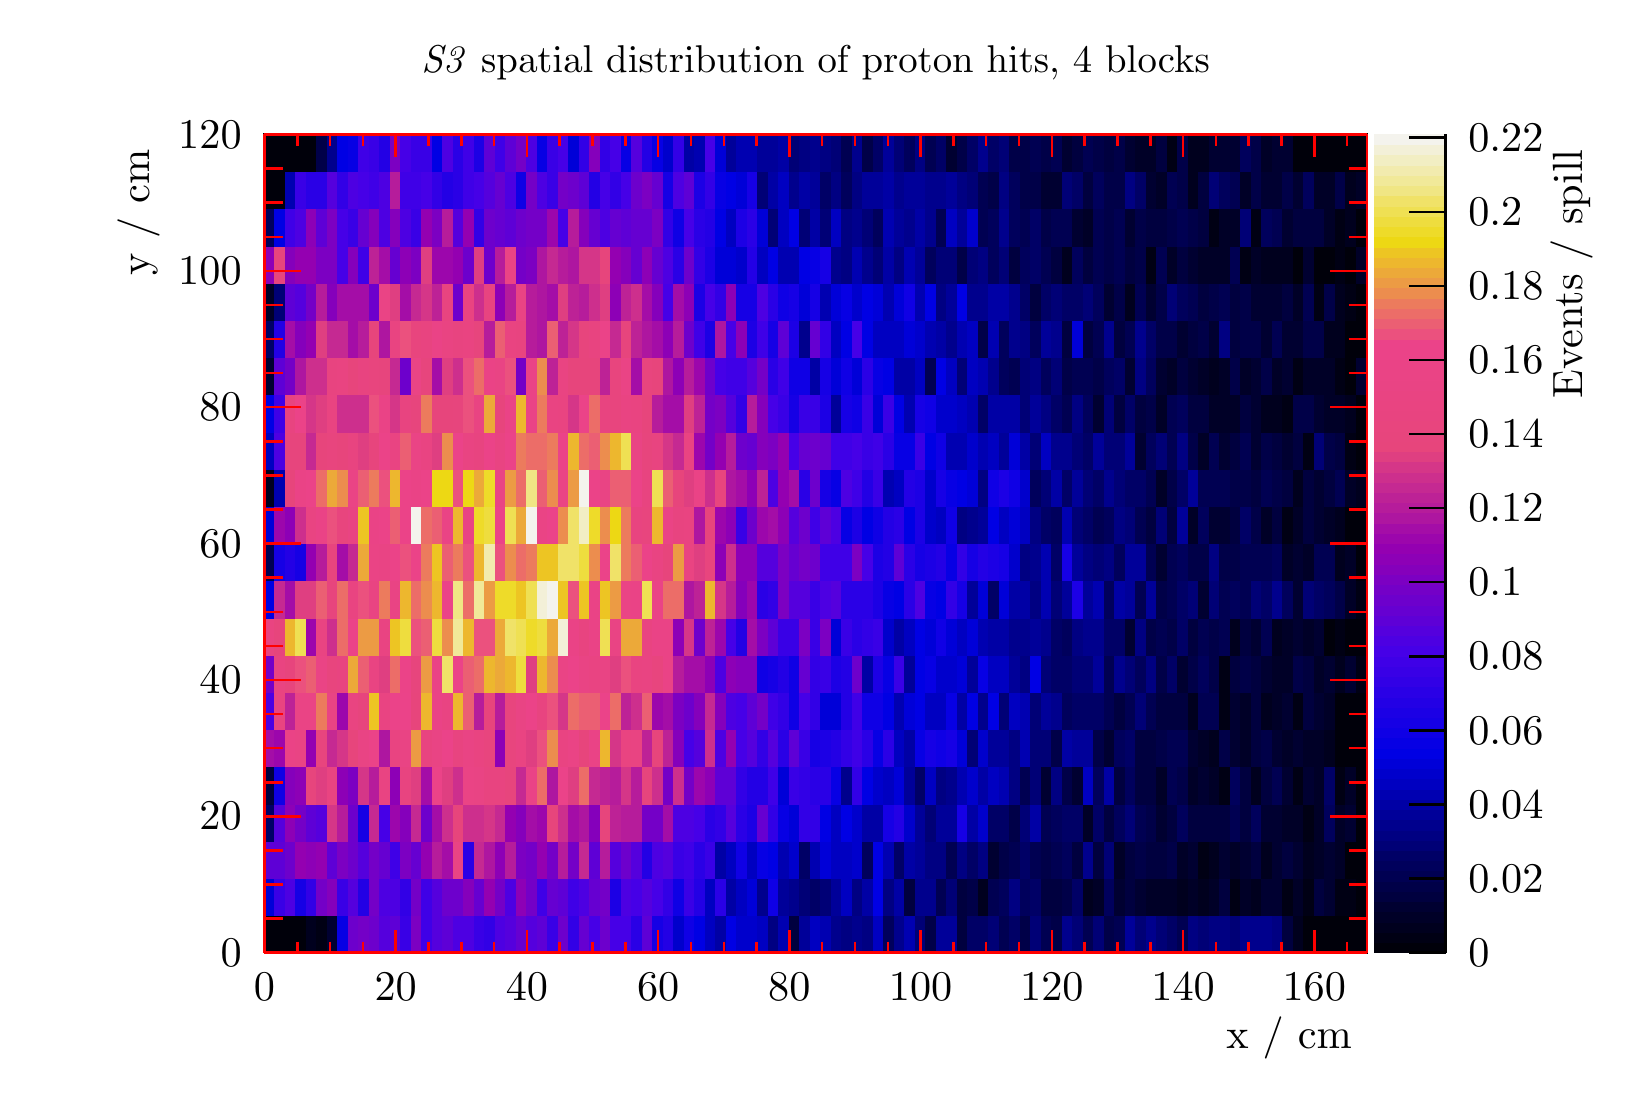
\begin{tikzpicture}
\pgfdeclareplotmark{cross} {
\pgfpathmoveto{\pgfpoint{-0.3\pgfplotmarksize}{\pgfplotmarksize}}
\pgfpathlineto{\pgfpoint{+0.3\pgfplotmarksize}{\pgfplotmarksize}}
\pgfpathlineto{\pgfpoint{+0.3\pgfplotmarksize}{0.3\pgfplotmarksize}}
\pgfpathlineto{\pgfpoint{+1\pgfplotmarksize}{0.3\pgfplotmarksize}}
\pgfpathlineto{\pgfpoint{+1\pgfplotmarksize}{-0.3\pgfplotmarksize}}
\pgfpathlineto{\pgfpoint{+0.3\pgfplotmarksize}{-0.3\pgfplotmarksize}}
\pgfpathlineto{\pgfpoint{+0.3\pgfplotmarksize}{-1.\pgfplotmarksize}}
\pgfpathlineto{\pgfpoint{-0.3\pgfplotmarksize}{-1.\pgfplotmarksize}}
\pgfpathlineto{\pgfpoint{-0.3\pgfplotmarksize}{-0.3\pgfplotmarksize}}
\pgfpathlineto{\pgfpoint{-1.\pgfplotmarksize}{-0.3\pgfplotmarksize}}
\pgfpathlineto{\pgfpoint{-1.\pgfplotmarksize}{0.3\pgfplotmarksize}}
\pgfpathlineto{\pgfpoint{-0.3\pgfplotmarksize}{0.3\pgfplotmarksize}}
\pgfpathclose
\pgfusepathqstroke
}
\pgfdeclareplotmark{cross*} {
\pgfpathmoveto{\pgfpoint{-0.3\pgfplotmarksize}{\pgfplotmarksize}}
\pgfpathlineto{\pgfpoint{+0.3\pgfplotmarksize}{\pgfplotmarksize}}
\pgfpathlineto{\pgfpoint{+0.3\pgfplotmarksize}{0.3\pgfplotmarksize}}
\pgfpathlineto{\pgfpoint{+1\pgfplotmarksize}{0.3\pgfplotmarksize}}
\pgfpathlineto{\pgfpoint{+1\pgfplotmarksize}{-0.3\pgfplotmarksize}}
\pgfpathlineto{\pgfpoint{+0.3\pgfplotmarksize}{-0.3\pgfplotmarksize}}
\pgfpathlineto{\pgfpoint{+0.3\pgfplotmarksize}{-1.\pgfplotmarksize}}
\pgfpathlineto{\pgfpoint{-0.3\pgfplotmarksize}{-1.\pgfplotmarksize}}
\pgfpathlineto{\pgfpoint{-0.3\pgfplotmarksize}{-0.3\pgfplotmarksize}}
\pgfpathlineto{\pgfpoint{-1.\pgfplotmarksize}{-0.3\pgfplotmarksize}}
\pgfpathlineto{\pgfpoint{-1.\pgfplotmarksize}{0.3\pgfplotmarksize}}
\pgfpathlineto{\pgfpoint{-0.3\pgfplotmarksize}{0.3\pgfplotmarksize}}
\pgfpathclose
\pgfusepathqfillstroke
}
\pgfdeclareplotmark{newstar} {
\pgfpathmoveto{\pgfqpoint{0pt}{\pgfplotmarksize}}
\pgfpathlineto{\pgfqpointpolar{44}{0.5\pgfplotmarksize}}
\pgfpathlineto{\pgfqpointpolar{18}{\pgfplotmarksize}}
\pgfpathlineto{\pgfqpointpolar{-20}{0.5\pgfplotmarksize}}
\pgfpathlineto{\pgfqpointpolar{-54}{\pgfplotmarksize}}
\pgfpathlineto{\pgfqpointpolar{-90}{0.5\pgfplotmarksize}}
\pgfpathlineto{\pgfqpointpolar{234}{\pgfplotmarksize}}
\pgfpathlineto{\pgfqpointpolar{198}{0.5\pgfplotmarksize}}
\pgfpathlineto{\pgfqpointpolar{162}{\pgfplotmarksize}}
\pgfpathlineto{\pgfqpointpolar{134}{0.5\pgfplotmarksize}}
\pgfpathclose
\pgfusepathqstroke
}
\pgfdeclareplotmark{newstar*} {
\pgfpathmoveto{\pgfqpoint{0pt}{\pgfplotmarksize}}
\pgfpathlineto{\pgfqpointpolar{44}{0.5\pgfplotmarksize}}
\pgfpathlineto{\pgfqpointpolar{18}{\pgfplotmarksize}}
\pgfpathlineto{\pgfqpointpolar{-20}{0.5\pgfplotmarksize}}
\pgfpathlineto{\pgfqpointpolar{-54}{\pgfplotmarksize}}
\pgfpathlineto{\pgfqpointpolar{-90}{0.5\pgfplotmarksize}}
\pgfpathlineto{\pgfqpointpolar{234}{\pgfplotmarksize}}
\pgfpathlineto{\pgfqpointpolar{198}{0.5\pgfplotmarksize}}
\pgfpathlineto{\pgfqpointpolar{162}{\pgfplotmarksize}}
\pgfpathlineto{\pgfqpointpolar{134}{0.5\pgfplotmarksize}}
\pgfpathclose
\pgfusepathqfillstroke
}
\definecolor{c}{rgb}{1,1,1};
\draw [color=c, fill=c] (0,0) rectangle (20,13.4957);
\draw [color=c, fill=c] (3,1.75444) rectangle (17,12.1461);
\definecolor{c}{rgb}{0,0,0};
\draw [c,line width=0.9] (3,1.75444) -- (3,12.1461) -- (17,12.1461) -- (17,1.75444) -- (3,1.75444);
\definecolor{c}{rgb}{1,1,1};
\draw [color=c, fill=c] (3,1.75444) rectangle (17,12.1461);
\definecolor{c}{rgb}{0,0,0};
\draw [c,line width=0.9] (3,1.75444) -- (3,12.1461) -- (17,12.1461) -- (17,1.75444) -- (3,1.75444);
\definecolor{c}{rgb}{0,0,0.0387097};
\draw [color=c, fill=c] (3,1.75444) rectangle (3.13333,2.22679);
\draw [color=c, fill=c] (3.13333,1.75444) rectangle (3.26667,2.22679);
\draw [color=c, fill=c] (3.26667,1.75444) rectangle (3.4,2.22679);
\draw [color=c, fill=c] (3.4,1.75444) rectangle (3.53333,2.22679);
\definecolor{c}{rgb}{0,0,0.116129};
\draw [color=c, fill=c] (3.53333,1.75444) rectangle (3.66667,2.22679);
\definecolor{c}{rgb}{0,0,0.0774194};
\draw [color=c, fill=c] (3.66667,1.75444) rectangle (3.8,2.22679);
\definecolor{c}{rgb}{0,0,0.193548};
\draw [color=c, fill=c] (3.8,1.75444) rectangle (3.93333,2.22679);
\definecolor{c}{rgb}{0.0257353,0,0.895221};
\draw [color=c, fill=c] (3.93333,1.75444) rectangle (4.06667,2.22679);
\definecolor{c}{rgb}{0.427451,0,0.8};
\draw [color=c, fill=c] (4.06667,1.75444) rectangle (4.2,2.22679);
\definecolor{c}{rgb}{0.456127,0,0.780147};
\draw [color=c, fill=c] (4.2,1.75444) rectangle (4.33333,2.22679);
\definecolor{c}{rgb}{0.427451,0,0.8};
\draw [color=c, fill=c] (4.33333,1.75444) rectangle (4.46667,2.22679);
\definecolor{c}{rgb}{0.331863,0,0.866176};
\draw [color=c, fill=c] (4.46667,1.75444) rectangle (4.6,2.22679);
\definecolor{c}{rgb}{0.370098,0,0.839706};
\draw [color=c, fill=c] (4.6,1.75444) rectangle (4.73333,2.22679);
\definecolor{c}{rgb}{0.223039,0,0.903676};
\draw [color=c, fill=c] (4.73333,1.75444) rectangle (4.86667,2.22679);
\definecolor{c}{rgb}{0.484804,0,0.760294};
\draw [color=c, fill=c] (4.86667,1.75444) rectangle (5,2.22679);
\definecolor{c}{rgb}{0.248775,0,0.904779};
\draw [color=c, fill=c] (5,1.75444) rectangle (5.13333,2.22679);
\definecolor{c}{rgb}{0.331863,0,0.866176};
\draw [color=c, fill=c] (5.13333,1.75444) rectangle (5.26667,2.22679);
\definecolor{c}{rgb}{0.370098,0,0.839706};
\draw [color=c, fill=c] (5.26667,1.75444) rectangle (5.4,2.22679);
\definecolor{c}{rgb}{0.303186,0,0.886029};
\draw [color=c, fill=c] (5.4,1.75444) rectangle (5.53333,2.22679);
\draw [color=c, fill=c] (5.53333,1.75444) rectangle (5.66667,2.22679);
\definecolor{c}{rgb}{0.223039,0,0.903676};
\draw [color=c, fill=c] (5.66667,1.75444) rectangle (5.8,2.22679);
\definecolor{c}{rgb}{0.197304,0,0.902574};
\draw [color=c, fill=c] (5.8,1.75444) rectangle (5.93333,2.22679);
\definecolor{c}{rgb}{0.303186,0,0.886029};
\draw [color=c, fill=c] (5.93333,1.75444) rectangle (6.06667,2.22679);
\definecolor{c}{rgb}{0.331863,0,0.866176};
\draw [color=c, fill=c] (6.06667,1.75444) rectangle (6.2,2.22679);
\definecolor{c}{rgb}{0.398775,0,0.819853};
\draw [color=c, fill=c] (6.2,1.75444) rectangle (6.33333,2.22679);
\definecolor{c}{rgb}{0.331863,0,0.866176};
\draw [color=c, fill=c] (6.33333,1.75444) rectangle (6.46667,2.22679);
\definecolor{c}{rgb}{0.370098,0,0.839706};
\draw [color=c, fill=c] (6.46667,1.75444) rectangle (6.6,2.22679);
\definecolor{c}{rgb}{0.223039,0,0.903676};
\draw [color=c, fill=c] (6.6,1.75444) rectangle (6.73333,2.22679);
\definecolor{c}{rgb}{0.427451,0,0.8};
\draw [color=c, fill=c] (6.73333,1.75444) rectangle (6.86667,2.22679);
\definecolor{c}{rgb}{0.197304,0,0.902574};
\draw [color=c, fill=c] (6.86667,1.75444) rectangle (7,2.22679);
\definecolor{c}{rgb}{0.398775,0,0.819853};
\draw [color=c, fill=c] (7,1.75444) rectangle (7.13333,2.22679);
\definecolor{c}{rgb}{0.27451,0,0.905882};
\draw [color=c, fill=c] (7.13333,1.75444) rectangle (7.26667,2.22679);
\definecolor{c}{rgb}{0.427451,0,0.8};
\draw [color=c, fill=c] (7.26667,1.75444) rectangle (7.4,2.22679);
\definecolor{c}{rgb}{0.27451,0,0.905882};
\draw [color=c, fill=c] (7.4,1.75444) rectangle (7.53333,2.22679);
\draw [color=c, fill=c] (7.53333,1.75444) rectangle (7.66667,2.22679);
\definecolor{c}{rgb}{0.16299,0,0.901103};
\draw [color=c, fill=c] (7.66667,1.75444) rectangle (7.8,2.22679);
\definecolor{c}{rgb}{0.370098,0,0.839706};
\draw [color=c, fill=c] (7.8,1.75444) rectangle (7.93333,2.22679);
\definecolor{c}{rgb}{0.0857843,0,0.897794};
\draw [color=c, fill=c] (7.93333,1.75444) rectangle (8.06667,2.22679);
\definecolor{c}{rgb}{0.137255,0,0.9};
\draw [color=c, fill=c] (8.06667,1.75444) rectangle (8.2,2.22679);
\definecolor{c}{rgb}{0,0,0.801471};
\draw [color=c, fill=c] (8.2,1.75444) rectangle (8.33333,2.22679);
\definecolor{c}{rgb}{0.060049,0,0.896691};
\draw [color=c, fill=c] (8.33333,1.75444) rectangle (8.46667,2.22679);
\definecolor{c}{rgb}{0,0,0.894118};
\draw [color=c, fill=c] (8.46667,1.75444) rectangle (8.6,2.22679);
\definecolor{c}{rgb}{0,0,0.755147};
\draw [color=c, fill=c] (8.6,1.75444) rectangle (8.73333,2.22679);
\definecolor{c}{rgb}{0,0,0.647059};
\draw [color=c, fill=c] (8.73333,1.75444) rectangle (8.86667,2.22679);
\definecolor{c}{rgb}{0,0,0.894118};
\draw [color=c, fill=c] (8.86667,1.75444) rectangle (9,2.22679);
\definecolor{c}{rgb}{0,0,0.801471};
\draw [color=c, fill=c] (9,1.75444) rectangle (9.13333,2.22679);
\draw [color=c, fill=c] (9.13333,1.75444) rectangle (9.26667,2.22679);
\definecolor{c}{rgb}{0,0,0.755147};
\draw [color=c, fill=c] (9.26667,1.75444) rectangle (9.4,2.22679);
\definecolor{c}{rgb}{0,0,0.508088};
\draw [color=c, fill=c] (9.4,1.75444) rectangle (9.53333,2.22679);
\definecolor{c}{rgb}{0,0,0.693382};
\draw [color=c, fill=c] (9.53333,1.75444) rectangle (9.66667,2.22679);
\definecolor{c}{rgb}{0,0,0.245161};
\draw [color=c, fill=c] (9.66667,1.75444) rectangle (9.8,2.22679);
\definecolor{c}{rgb}{0,0,0.600735};
\draw [color=c, fill=c] (9.8,1.75444) rectangle (9.93333,2.22679);
\definecolor{c}{rgb}{0,0,0.755147};
\draw [color=c, fill=c] (9.93333,1.75444) rectangle (10.0667,2.22679);
\definecolor{c}{rgb}{0,0,0.693382};
\draw [color=c, fill=c] (10.0667,1.75444) rectangle (10.2,2.22679);
\definecolor{c}{rgb}{0,0,0.554412};
\draw [color=c, fill=c] (10.2,1.75444) rectangle (10.3333,2.22679);
\definecolor{c}{rgb}{0,0,0.508088};
\draw [color=c, fill=c] (10.3333,1.75444) rectangle (10.4667,2.22679);
\definecolor{c}{rgb}{0,0,0.554412};
\draw [color=c, fill=c] (10.4667,1.75444) rectangle (10.6,2.22679);
\definecolor{c}{rgb}{0,0,0.508088};
\draw [color=c, fill=c] (10.6,1.75444) rectangle (10.7333,2.22679);
\definecolor{c}{rgb}{0,0,0.755147};
\draw [color=c, fill=c] (10.7333,1.75444) rectangle (10.8667,2.22679);
\definecolor{c}{rgb}{0,0,0.36129};
\draw [color=c, fill=c] (10.8667,1.75444) rectangle (11,2.22679);
\definecolor{c}{rgb}{0,0,0.554412};
\draw [color=c, fill=c] (11,1.75444) rectangle (11.1333,2.22679);
\definecolor{c}{rgb}{0,0,0.693382};
\draw [color=c, fill=c] (11.1333,1.75444) rectangle (11.2667,2.22679);
\definecolor{c}{rgb}{0,0,0.461765};
\draw [color=c, fill=c] (11.2667,1.75444) rectangle (11.4,2.22679);
\definecolor{c}{rgb}{0,0,0.283871};
\draw [color=c, fill=c] (11.4,1.75444) rectangle (11.5333,2.22679);
\definecolor{c}{rgb}{0,0,0.600735};
\draw [color=c, fill=c] (11.5333,1.75444) rectangle (11.6667,2.22679);
\draw [color=c, fill=c] (11.6667,1.75444) rectangle (11.8,2.22679);
\definecolor{c}{rgb}{0,0,0.245161};
\draw [color=c, fill=c] (11.8,1.75444) rectangle (11.9333,2.22679);
\definecolor{c}{rgb}{0,0,0.4};
\draw [color=c, fill=c] (11.9333,1.75444) rectangle (12.0667,2.22679);
\draw [color=c, fill=c] (12.0667,1.75444) rectangle (12.2,2.22679);
\definecolor{c}{rgb}{0,0,0.461765};
\draw [color=c, fill=c] (12.2,1.75444) rectangle (12.3333,2.22679);
\definecolor{c}{rgb}{0,0,0.322581};
\draw [color=c, fill=c] (12.3333,1.75444) rectangle (12.4667,2.22679);
\definecolor{c}{rgb}{0,0,0.4};
\draw [color=c, fill=c] (12.4667,1.75444) rectangle (12.6,2.22679);
\definecolor{c}{rgb}{0,0,0.283871};
\draw [color=c, fill=c] (12.6,1.75444) rectangle (12.7333,2.22679);
\definecolor{c}{rgb}{0,0,0.461765};
\draw [color=c, fill=c] (12.7333,1.75444) rectangle (12.8667,2.22679);
\definecolor{c}{rgb}{0,0,0.322581};
\draw [color=c, fill=c] (12.8667,1.75444) rectangle (13,2.22679);
\definecolor{c}{rgb}{0,0,0.283871};
\draw [color=c, fill=c] (13,1.75444) rectangle (13.1333,2.22679);
\definecolor{c}{rgb}{0,0,0.554412};
\draw [color=c, fill=c] (13.1333,1.75444) rectangle (13.2667,2.22679);
\definecolor{c}{rgb}{0,0,0.461765};
\draw [color=c, fill=c] (13.2667,1.75444) rectangle (13.4,2.22679);
\definecolor{c}{rgb}{0,0,0.322581};
\draw [color=c, fill=c] (13.4,1.75444) rectangle (13.5333,2.22679);
\definecolor{c}{rgb}{0,0,0.461765};
\draw [color=c, fill=c] (13.5333,1.75444) rectangle (13.6667,2.22679);
\definecolor{c}{rgb}{0,0,0.283871};
\draw [color=c, fill=c] (13.6667,1.75444) rectangle (13.8,2.22679);
\definecolor{c}{rgb}{0,0,0.322581};
\draw [color=c, fill=c] (13.8,1.75444) rectangle (13.9333,2.22679);
\definecolor{c}{rgb}{0,0,0.600735};
\draw [color=c, fill=c] (13.9333,1.75444) rectangle (14.0667,2.22679);
\definecolor{c}{rgb}{0,0,0.461765};
\draw [color=c, fill=c] (14.0667,1.75444) rectangle (14.2,2.22679);
\definecolor{c}{rgb}{0,0,0.554412};
\draw [color=c, fill=c] (14.2,1.75444) rectangle (14.3333,2.22679);
\definecolor{c}{rgb}{0,0,0.461765};
\draw [color=c, fill=c] (14.3333,1.75444) rectangle (14.4667,2.22679);
\definecolor{c}{rgb}{0,0,0.4};
\draw [color=c, fill=c] (14.4667,1.75444) rectangle (14.6,2.22679);
\definecolor{c}{rgb}{0,0,0.322581};
\draw [color=c, fill=c] (14.6,1.75444) rectangle (14.7333,2.22679);
\definecolor{c}{rgb}{0,0,0.508088};
\draw [color=c, fill=c] (14.7333,1.75444) rectangle (14.8667,2.22679);
\definecolor{c}{rgb}{0,0,0.461765};
\draw [color=c, fill=c] (14.8667,1.75444) rectangle (15,2.22679);
\definecolor{c}{rgb}{0,0,0.508088};
\draw [color=c, fill=c] (15,1.75444) rectangle (15.1333,2.22679);
\draw [color=c, fill=c] (15.1333,1.75444) rectangle (15.2667,2.22679);
\definecolor{c}{rgb}{0,0,0.461765};
\draw [color=c, fill=c] (15.2667,1.75444) rectangle (15.4,2.22679);
\definecolor{c}{rgb}{0,0,0.554412};
\draw [color=c, fill=c] (15.4,1.75444) rectangle (15.5333,2.22679);
\draw [color=c, fill=c] (15.5333,1.75444) rectangle (15.6667,2.22679);
\draw [color=c, fill=c] (15.6667,1.75444) rectangle (15.8,2.22679);
\definecolor{c}{rgb}{0,0,0.508088};
\draw [color=c, fill=c] (15.8,1.75444) rectangle (15.9333,2.22679);
\definecolor{c}{rgb}{0,0,0.245161};
\draw [color=c, fill=c] (15.9333,1.75444) rectangle (16.0667,2.22679);
\definecolor{c}{rgb}{0,0,0.116129};
\draw [color=c, fill=c] (16.0667,1.75444) rectangle (16.2,2.22679);
\definecolor{c}{rgb}{0,0,0.0387097};
\draw [color=c, fill=c] (16.2,1.75444) rectangle (16.3333,2.22679);
\draw [color=c, fill=c] (16.3333,1.75444) rectangle (16.4667,2.22679);
\draw [color=c, fill=c] (16.4667,1.75444) rectangle (16.6,2.22679);
\draw [color=c, fill=c] (16.6,1.75444) rectangle (16.7333,2.22679);
\draw [color=c, fill=c] (16.7333,1.75444) rectangle (16.8667,2.22679);
\draw [color=c, fill=c] (16.8667,1.75444) rectangle (17,2.22679);
\definecolor{c}{rgb}{0,0,0.847794};
\draw [color=c, fill=c] (3,2.22679) rectangle (3.13333,2.69914);
\definecolor{c}{rgb}{0.223039,0,0.903676};
\draw [color=c, fill=c] (3.13333,2.22679) rectangle (3.26667,2.69914);
\definecolor{c}{rgb}{0.303186,0,0.886029};
\draw [color=c, fill=c] (3.26667,2.22679) rectangle (3.4,2.69914);
\definecolor{c}{rgb}{0.0857843,0,0.897794};
\draw [color=c, fill=c] (3.4,2.22679) rectangle (3.53333,2.69914);
\definecolor{c}{rgb}{0.197304,0,0.902574};
\draw [color=c, fill=c] (3.53333,2.22679) rectangle (3.66667,2.69914);
\definecolor{c}{rgb}{0.456127,0,0.780147};
\draw [color=c, fill=c] (3.66667,2.22679) rectangle (3.8,2.69914);
\definecolor{c}{rgb}{0.523039,0,0.733824};
\draw [color=c, fill=c] (3.8,2.22679) rectangle (3.93333,2.69914);
\definecolor{c}{rgb}{0.223039,0,0.903676};
\draw [color=c, fill=c] (3.93333,2.22679) rectangle (4.06667,2.69914);
\definecolor{c}{rgb}{0.331863,0,0.866176};
\draw [color=c, fill=c] (4.06667,2.22679) rectangle (4.2,2.69914);
\definecolor{c}{rgb}{0.137255,0,0.9};
\draw [color=c, fill=c] (4.2,2.22679) rectangle (4.33333,2.69914);
\definecolor{c}{rgb}{0.456127,0,0.780147};
\draw [color=c, fill=c] (4.33333,2.22679) rectangle (4.46667,2.69914);
\definecolor{c}{rgb}{0.303186,0,0.886029};
\draw [color=c, fill=c] (4.46667,2.22679) rectangle (4.6,2.69914);
\draw [color=c, fill=c] (4.6,2.22679) rectangle (4.73333,2.69914);
\definecolor{c}{rgb}{0.197304,0,0.902574};
\draw [color=c, fill=c] (4.73333,2.22679) rectangle (4.86667,2.69914);
\definecolor{c}{rgb}{0.456127,0,0.780147};
\draw [color=c, fill=c] (4.86667,2.22679) rectangle (5,2.69914);
\definecolor{c}{rgb}{0.248775,0,0.904779};
\draw [color=c, fill=c] (5,2.22679) rectangle (5.13333,2.69914);
\definecolor{c}{rgb}{0.331863,0,0.866176};
\draw [color=c, fill=c] (5.13333,2.22679) rectangle (5.26667,2.69914);
\definecolor{c}{rgb}{0.427451,0,0.8};
\draw [color=c, fill=c] (5.26667,2.22679) rectangle (5.4,2.69914);
\draw [color=c, fill=c] (5.4,2.22679) rectangle (5.53333,2.69914);
\definecolor{c}{rgb}{0.523039,0,0.733824};
\draw [color=c, fill=c] (5.53333,2.22679) rectangle (5.66667,2.69914);
\definecolor{c}{rgb}{0.398775,0,0.819853};
\draw [color=c, fill=c] (5.66667,2.22679) rectangle (5.8,2.69914);
\definecolor{c}{rgb}{0.580392,0,0.694118};
\draw [color=c, fill=c] (5.8,2.22679) rectangle (5.93333,2.69914);
\definecolor{c}{rgb}{0.456127,0,0.780147};
\draw [color=c, fill=c] (5.93333,2.22679) rectangle (6.06667,2.69914);
\definecolor{c}{rgb}{0.303186,0,0.886029};
\draw [color=c, fill=c] (6.06667,2.22679) rectangle (6.2,2.69914);
\definecolor{c}{rgb}{0.551716,0,0.713971};
\draw [color=c, fill=c] (6.2,2.22679) rectangle (6.33333,2.69914);
\definecolor{c}{rgb}{0.456127,0,0.780147};
\draw [color=c, fill=c] (6.33333,2.22679) rectangle (6.46667,2.69914);
\definecolor{c}{rgb}{0.248775,0,0.904779};
\draw [color=c, fill=c] (6.46667,2.22679) rectangle (6.6,2.69914);
\definecolor{c}{rgb}{0.398775,0,0.819853};
\draw [color=c, fill=c] (6.6,2.22679) rectangle (6.73333,2.69914);
\definecolor{c}{rgb}{0.370098,0,0.839706};
\draw [color=c, fill=c] (6.73333,2.22679) rectangle (6.86667,2.69914);
\definecolor{c}{rgb}{0.248775,0,0.904779};
\draw [color=c, fill=c] (6.86667,2.22679) rectangle (7,2.69914);
\definecolor{c}{rgb}{0.303186,0,0.886029};
\draw [color=c, fill=c] (7,2.22679) rectangle (7.13333,2.69914);
\definecolor{c}{rgb}{0.398775,0,0.819853};
\draw [color=c, fill=c] (7.13333,2.22679) rectangle (7.26667,2.69914);
\definecolor{c}{rgb}{0.456127,0,0.780147};
\draw [color=c, fill=c] (7.26667,2.22679) rectangle (7.4,2.69914);
\definecolor{c}{rgb}{0.11152,0,0.898897};
\draw [color=c, fill=c] (7.4,2.22679) rectangle (7.53333,2.69914);
\definecolor{c}{rgb}{0.303186,0,0.886029};
\draw [color=c, fill=c] (7.53333,2.22679) rectangle (7.66667,2.69914);
\definecolor{c}{rgb}{0.27451,0,0.905882};
\draw [color=c, fill=c] (7.66667,2.22679) rectangle (7.8,2.69914);
\definecolor{c}{rgb}{0.331863,0,0.866176};
\draw [color=c, fill=c] (7.8,2.22679) rectangle (7.93333,2.69914);
\definecolor{c}{rgb}{0.27451,0,0.905882};
\draw [color=c, fill=c] (7.93333,2.22679) rectangle (8.06667,2.69914);
\definecolor{c}{rgb}{0.197304,0,0.902574};
\draw [color=c, fill=c] (8.06667,2.22679) rectangle (8.2,2.69914);
\definecolor{c}{rgb}{0.060049,0,0.896691};
\draw [color=c, fill=c] (8.2,2.22679) rectangle (8.33333,2.69914);
\definecolor{c}{rgb}{0.223039,0,0.903676};
\draw [color=c, fill=c] (8.33333,2.22679) rectangle (8.46667,2.69914);
\definecolor{c}{rgb}{0.137255,0,0.9};
\draw [color=c, fill=c] (8.46667,2.22679) rectangle (8.6,2.69914);
\definecolor{c}{rgb}{0,0,0.755147};
\draw [color=c, fill=c] (8.6,2.22679) rectangle (8.73333,2.69914);
\definecolor{c}{rgb}{0.16299,0,0.901103};
\draw [color=c, fill=c] (8.73333,2.22679) rectangle (8.86667,2.69914);
\definecolor{c}{rgb}{0,0,0.647059};
\draw [color=c, fill=c] (8.86667,2.22679) rectangle (9,2.69914);
\definecolor{c}{rgb}{0,0,0.755147};
\draw [color=c, fill=c] (9,2.22679) rectangle (9.13333,2.69914);
\definecolor{c}{rgb}{0,0,0.847794};
\draw [color=c, fill=c] (9.13333,2.22679) rectangle (9.26667,2.69914);
\definecolor{c}{rgb}{0,0,0.554412};
\draw [color=c, fill=c] (9.26667,2.22679) rectangle (9.4,2.69914);
\definecolor{c}{rgb}{0.060049,0,0.896691};
\draw [color=c, fill=c] (9.4,2.22679) rectangle (9.53333,2.69914);
\definecolor{c}{rgb}{0,0,0.600735};
\draw [color=c, fill=c] (9.53333,2.22679) rectangle (9.66667,2.69914);
\definecolor{c}{rgb}{0,0,0.554412};
\draw [color=c, fill=c] (9.66667,2.22679) rectangle (9.8,2.69914);
\definecolor{c}{rgb}{0,0,0.461765};
\draw [color=c, fill=c] (9.8,2.22679) rectangle (9.93333,2.69914);
\definecolor{c}{rgb}{0,0,0.4};
\draw [color=c, fill=c] (9.93333,2.22679) rectangle (10.0667,2.69914);
\definecolor{c}{rgb}{0,0,0.461765};
\draw [color=c, fill=c] (10.0667,2.22679) rectangle (10.2,2.69914);
\definecolor{c}{rgb}{0,0,0.600735};
\draw [color=c, fill=c] (10.2,2.22679) rectangle (10.3333,2.69914);
\definecolor{c}{rgb}{0,0,0.755147};
\draw [color=c, fill=c] (10.3333,2.22679) rectangle (10.4667,2.69914);
\definecolor{c}{rgb}{0,0,0.508088};
\draw [color=c, fill=c] (10.4667,2.22679) rectangle (10.6,2.69914);
\definecolor{c}{rgb}{0,0,0.647059};
\draw [color=c, fill=c] (10.6,2.22679) rectangle (10.7333,2.69914);
\definecolor{c}{rgb}{0,0,0.894118};
\draw [color=c, fill=c] (10.7333,2.22679) rectangle (10.8667,2.69914);
\definecolor{c}{rgb}{0,0,0.508088};
\draw [color=c, fill=c] (10.8667,2.22679) rectangle (11,2.69914);
\definecolor{c}{rgb}{0,0,0.647059};
\draw [color=c, fill=c] (11,2.22679) rectangle (11.1333,2.69914);
\definecolor{c}{rgb}{0,0,0.245161};
\draw [color=c, fill=c] (11.1333,2.22679) rectangle (11.2667,2.69914);
\definecolor{c}{rgb}{0,0,0.554412};
\draw [color=c, fill=c] (11.2667,2.22679) rectangle (11.4,2.69914);
\draw [color=c, fill=c] (11.4,2.22679) rectangle (11.5333,2.69914);
\definecolor{c}{rgb}{0,0,0.322581};
\draw [color=c, fill=c] (11.5333,2.22679) rectangle (11.6667,2.69914);
\definecolor{c}{rgb}{0,0,0.461765};
\draw [color=c, fill=c] (11.6667,2.22679) rectangle (11.8,2.69914);
\definecolor{c}{rgb}{0,0,0.245161};
\draw [color=c, fill=c] (11.8,2.22679) rectangle (11.9333,2.69914);
\definecolor{c}{rgb}{0,0,0.283871};
\draw [color=c, fill=c] (11.9333,2.22679) rectangle (12.0667,2.69914);
\definecolor{c}{rgb}{0,0,0.116129};
\draw [color=c, fill=c] (12.0667,2.22679) rectangle (12.2,2.69914);
\definecolor{c}{rgb}{0,0,0.322581};
\draw [color=c, fill=c] (12.2,2.22679) rectangle (12.3333,2.69914);
\definecolor{c}{rgb}{0,0,0.36129};
\draw [color=c, fill=c] (12.3333,2.22679) rectangle (12.4667,2.69914);
\definecolor{c}{rgb}{0,0,0.508088};
\draw [color=c, fill=c] (12.4667,2.22679) rectangle (12.6,2.69914);
\definecolor{c}{rgb}{0,0,0.36129};
\draw [color=c, fill=c] (12.6,2.22679) rectangle (12.7333,2.69914);
\definecolor{c}{rgb}{0,0,0.4};
\draw [color=c, fill=c] (12.7333,2.22679) rectangle (12.8667,2.69914);
\definecolor{c}{rgb}{0,0,0.245161};
\draw [color=c, fill=c] (12.8667,2.22679) rectangle (13,2.69914);
\draw [color=c, fill=c] (13,2.22679) rectangle (13.1333,2.69914);
\definecolor{c}{rgb}{0,0,0.283871};
\draw [color=c, fill=c] (13.1333,2.22679) rectangle (13.2667,2.69914);
\definecolor{c}{rgb}{0,0,0.4};
\draw [color=c, fill=c] (13.2667,2.22679) rectangle (13.4,2.69914);
\definecolor{c}{rgb}{0,0,0.116129};
\draw [color=c, fill=c] (13.4,2.22679) rectangle (13.5333,2.69914);
\definecolor{c}{rgb}{0,0,0.154839};
\draw [color=c, fill=c] (13.5333,2.22679) rectangle (13.6667,2.69914);
\definecolor{c}{rgb}{0,0,0.36129};
\draw [color=c, fill=c] (13.6667,2.22679) rectangle (13.8,2.69914);
\definecolor{c}{rgb}{0,0,0.193548};
\draw [color=c, fill=c] (13.8,2.22679) rectangle (13.9333,2.69914);
\definecolor{c}{rgb}{0,0,0.245161};
\draw [color=c, fill=c] (13.9333,2.22679) rectangle (14.0667,2.69914);
\definecolor{c}{rgb}{0,0,0.193548};
\draw [color=c, fill=c] (14.0667,2.22679) rectangle (14.2,2.69914);
\definecolor{c}{rgb}{0,0,0.154839};
\draw [color=c, fill=c] (14.2,2.22679) rectangle (14.3333,2.69914);
\draw [color=c, fill=c] (14.3333,2.22679) rectangle (14.4667,2.69914);
\draw [color=c, fill=c] (14.4667,2.22679) rectangle (14.6,2.69914);
\definecolor{c}{rgb}{0,0,0.116129};
\draw [color=c, fill=c] (14.6,2.22679) rectangle (14.7333,2.69914);
\definecolor{c}{rgb}{0,0,0.154839};
\draw [color=c, fill=c] (14.7333,2.22679) rectangle (14.8667,2.69914);
\definecolor{c}{rgb}{0,0,0.116129};
\draw [color=c, fill=c] (14.8667,2.22679) rectangle (15,2.69914);
\definecolor{c}{rgb}{0,0,0.154839};
\draw [color=c, fill=c] (15,2.22679) rectangle (15.1333,2.69914);
\definecolor{c}{rgb}{0,0,0.245161};
\draw [color=c, fill=c] (15.1333,2.22679) rectangle (15.2667,2.69914);
\definecolor{c}{rgb}{0,0,0.0774194};
\draw [color=c, fill=c] (15.2667,2.22679) rectangle (15.4,2.69914);
\definecolor{c}{rgb}{0,0,0.154839};
\draw [color=c, fill=c] (15.4,2.22679) rectangle (15.5333,2.69914);
\definecolor{c}{rgb}{0,0,0.116129};
\draw [color=c, fill=c] (15.5333,2.22679) rectangle (15.6667,2.69914);
\definecolor{c}{rgb}{0,0,0.193548};
\draw [color=c, fill=c] (15.6667,2.22679) rectangle (15.8,2.69914);
\draw [color=c, fill=c] (15.8,2.22679) rectangle (15.9333,2.69914);
\definecolor{c}{rgb}{0,0,0.0774194};
\draw [color=c, fill=c] (15.9333,2.22679) rectangle (16.0667,2.69914);
\definecolor{c}{rgb}{0,0,0.154839};
\draw [color=c, fill=c] (16.0667,2.22679) rectangle (16.2,2.69914);
\definecolor{c}{rgb}{0,0,0.0774194};
\draw [color=c, fill=c] (16.2,2.22679) rectangle (16.3333,2.69914);
\definecolor{c}{rgb}{0,0,0.245161};
\draw [color=c, fill=c] (16.3333,2.22679) rectangle (16.4667,2.69914);
\definecolor{c}{rgb}{0,0,0.193548};
\draw [color=c, fill=c] (16.4667,2.22679) rectangle (16.6,2.69914);
\definecolor{c}{rgb}{0,0,0.0774194};
\draw [color=c, fill=c] (16.6,2.22679) rectangle (16.7333,2.69914);
\draw [color=c, fill=c] (16.7333,2.22679) rectangle (16.8667,2.69914);
\definecolor{c}{rgb}{0,0,0.0387097};
\draw [color=c, fill=c] (16.8667,2.22679) rectangle (17,2.69914);
\definecolor{c}{rgb}{0.370098,0,0.839706};
\draw [color=c, fill=c] (3,2.69914) rectangle (3.13333,3.17149);
\draw [color=c, fill=c] (3.13333,2.69914) rectangle (3.26667,3.17149);
\definecolor{c}{rgb}{0.427451,0,0.8};
\draw [color=c, fill=c] (3.26667,2.69914) rectangle (3.4,3.17149);
\definecolor{c}{rgb}{0.580392,0,0.694118};
\draw [color=c, fill=c] (3.4,2.69914) rectangle (3.53333,3.17149);
\definecolor{c}{rgb}{0.551716,0,0.713971};
\draw [color=c, fill=c] (3.53333,2.69914) rectangle (3.66667,3.17149);
\definecolor{c}{rgb}{0.580392,0,0.694118};
\draw [color=c, fill=c] (3.66667,2.69914) rectangle (3.8,3.17149);
\definecolor{c}{rgb}{0.370098,0,0.839706};
\draw [color=c, fill=c] (3.8,2.69914) rectangle (3.93333,3.17149);
\definecolor{c}{rgb}{0.484804,0,0.760294};
\draw [color=c, fill=c] (3.93333,2.69914) rectangle (4.06667,3.17149);
\definecolor{c}{rgb}{0.427451,0,0.8};
\draw [color=c, fill=c] (4.06667,2.69914) rectangle (4.2,3.17149);
\definecolor{c}{rgb}{0.331863,0,0.866176};
\draw [color=c, fill=c] (4.2,2.69914) rectangle (4.33333,3.17149);
\definecolor{c}{rgb}{0.456127,0,0.780147};
\draw [color=c, fill=c] (4.33333,2.69914) rectangle (4.46667,3.17149);
\definecolor{c}{rgb}{0.398775,0,0.819853};
\draw [color=c, fill=c] (4.46667,2.69914) rectangle (4.6,3.17149);
\definecolor{c}{rgb}{0.248775,0,0.904779};
\draw [color=c, fill=c] (4.6,2.69914) rectangle (4.73333,3.17149);
\definecolor{c}{rgb}{0.484804,0,0.760294};
\draw [color=c, fill=c] (4.73333,2.69914) rectangle (4.86667,3.17149);
\definecolor{c}{rgb}{0.398775,0,0.819853};
\draw [color=c, fill=c] (4.86667,2.69914) rectangle (5,3.17149);
\definecolor{c}{rgb}{0.580392,0,0.694118};
\draw [color=c, fill=c] (5,2.69914) rectangle (5.13333,3.17149);
\definecolor{c}{rgb}{0.712623,0.109926,0.609681};
\draw [color=c, fill=c] (5.13333,2.69914) rectangle (5.26667,3.17149);
\definecolor{c}{rgb}{0.641422,0.0507353,0.655147};
\draw [color=c, fill=c] (5.26667,2.69914) rectangle (5.4,3.17149);
\definecolor{c}{rgb}{0.915196,0.265931,0.516544};
\draw [color=c, fill=c] (5.4,2.69914) rectangle (5.53333,3.17149);
\definecolor{c}{rgb}{0.16299,0,0.901103};
\draw [color=c, fill=c] (5.53333,2.69914) rectangle (5.66667,3.17149);
\definecolor{c}{rgb}{0.773652,0.160662,0.570711};
\draw [color=c, fill=c] (5.66667,2.69914) rectangle (5.8,3.17149);
\definecolor{c}{rgb}{0.682108,0.0845588,0.629167};
\draw [color=c, fill=c] (5.8,2.69914) rectangle (5.93333,3.17149);
\definecolor{c}{rgb}{0.551716,0,0.713971};
\draw [color=c, fill=c] (5.93333,2.69914) rectangle (6.06667,3.17149);
\definecolor{c}{rgb}{0.712623,0.109926,0.609681};
\draw [color=c, fill=c] (6.06667,2.69914) rectangle (6.2,3.17149);
\definecolor{c}{rgb}{0.484804,0,0.760294};
\draw [color=c, fill=c] (6.2,2.69914) rectangle (6.33333,3.17149);
\definecolor{c}{rgb}{0.456127,0,0.780147};
\draw [color=c, fill=c] (6.33333,2.69914) rectangle (6.46667,3.17149);
\definecolor{c}{rgb}{0.580392,0,0.694118};
\draw [color=c, fill=c] (6.46667,2.69914) rectangle (6.6,3.17149);
\definecolor{c}{rgb}{0.456127,0,0.780147};
\draw [color=c, fill=c] (6.6,2.69914) rectangle (6.73333,3.17149);
\definecolor{c}{rgb}{0.712623,0.109926,0.609681};
\draw [color=c, fill=c] (6.73333,2.69914) rectangle (6.86667,3.17149);
\definecolor{c}{rgb}{0.456127,0,0.780147};
\draw [color=c, fill=c] (6.86667,2.69914) rectangle (7,3.17149);
\definecolor{c}{rgb}{0.773652,0.160662,0.570711};
\draw [color=c, fill=c] (7,2.69914) rectangle (7.13333,3.17149);
\definecolor{c}{rgb}{0.370098,0,0.839706};
\draw [color=c, fill=c] (7.13333,2.69914) rectangle (7.26667,3.17149);
\definecolor{c}{rgb}{0.712623,0.109926,0.609681};
\draw [color=c, fill=c] (7.26667,2.69914) rectangle (7.4,3.17149);
\definecolor{c}{rgb}{0.331863,0,0.866176};
\draw [color=c, fill=c] (7.4,2.69914) rectangle (7.53333,3.17149);
\definecolor{c}{rgb}{0.427451,0,0.8};
\draw [color=c, fill=c] (7.53333,2.69914) rectangle (7.66667,3.17149);
\definecolor{c}{rgb}{0.331863,0,0.866176};
\draw [color=c, fill=c] (7.66667,2.69914) rectangle (7.8,3.17149);
\definecolor{c}{rgb}{0.137255,0,0.9};
\draw [color=c, fill=c] (7.8,2.69914) rectangle (7.93333,3.17149);
\definecolor{c}{rgb}{0.303186,0,0.886029};
\draw [color=c, fill=c] (7.93333,2.69914) rectangle (8.06667,3.17149);
\definecolor{c}{rgb}{0.331863,0,0.866176};
\draw [color=c, fill=c] (8.06667,2.69914) rectangle (8.2,3.17149);
\definecolor{c}{rgb}{0.223039,0,0.903676};
\draw [color=c, fill=c] (8.2,2.69914) rectangle (8.33333,3.17149);
\definecolor{c}{rgb}{0.248775,0,0.904779};
\draw [color=c, fill=c] (8.33333,2.69914) rectangle (8.46667,3.17149);
\definecolor{c}{rgb}{0.16299,0,0.901103};
\draw [color=c, fill=c] (8.46667,2.69914) rectangle (8.6,3.17149);
\definecolor{c}{rgb}{0.223039,0,0.903676};
\draw [color=c, fill=c] (8.6,2.69914) rectangle (8.73333,3.17149);
\definecolor{c}{rgb}{0,0,0.647059};
\draw [color=c, fill=c] (8.73333,2.69914) rectangle (8.86667,3.17149);
\definecolor{c}{rgb}{0,0,0.755147};
\draw [color=c, fill=c] (8.86667,2.69914) rectangle (9,3.17149);
\definecolor{c}{rgb}{0.060049,0,0.896691};
\draw [color=c, fill=c] (9,2.69914) rectangle (9.13333,3.17149);
\definecolor{c}{rgb}{0,0,0.755147};
\draw [color=c, fill=c] (9.13333,2.69914) rectangle (9.26667,3.17149);
\definecolor{c}{rgb}{0.0257353,0,0.895221};
\draw [color=c, fill=c] (9.26667,2.69914) rectangle (9.4,3.17149);
\definecolor{c}{rgb}{0,0,0.894118};
\draw [color=c, fill=c] (9.4,2.69914) rectangle (9.53333,3.17149);
\definecolor{c}{rgb}{0,0,0.693382};
\draw [color=c, fill=c] (9.53333,2.69914) rectangle (9.66667,3.17149);
\definecolor{c}{rgb}{0,0,0.801471};
\draw [color=c, fill=c] (9.66667,2.69914) rectangle (9.8,3.17149);
\definecolor{c}{rgb}{0,0,0.4};
\draw [color=c, fill=c] (9.8,2.69914) rectangle (9.93333,3.17149);
\definecolor{c}{rgb}{0,0,0.693382};
\draw [color=c, fill=c] (9.93333,2.69914) rectangle (10.0667,3.17149);
\definecolor{c}{rgb}{0,0,0.847794};
\draw [color=c, fill=c] (10.0667,2.69914) rectangle (10.2,3.17149);
\definecolor{c}{rgb}{0,0,0.755147};
\draw [color=c, fill=c] (10.2,2.69914) rectangle (10.3333,3.17149);
\draw [color=c, fill=c] (10.3333,2.69914) rectangle (10.4667,3.17149);
\definecolor{c}{rgb}{0,0,0.801471};
\draw [color=c, fill=c] (10.4667,2.69914) rectangle (10.6,3.17149);
\definecolor{c}{rgb}{0,0,0.36129};
\draw [color=c, fill=c] (10.6,2.69914) rectangle (10.7333,3.17149);
\definecolor{c}{rgb}{0,0,0.894118};
\draw [color=c, fill=c] (10.7333,2.69914) rectangle (10.8667,3.17149);
\definecolor{c}{rgb}{0,0,0.693382};
\draw [color=c, fill=c] (10.8667,2.69914) rectangle (11,3.17149);
\definecolor{c}{rgb}{0,0,0.4};
\draw [color=c, fill=c] (11,2.69914) rectangle (11.1333,3.17149);
\definecolor{c}{rgb}{0,0,0.647059};
\draw [color=c, fill=c] (11.1333,2.69914) rectangle (11.2667,3.17149);
\definecolor{c}{rgb}{0,0,0.600735};
\draw [color=c, fill=c] (11.2667,2.69914) rectangle (11.4,3.17149);
\definecolor{c}{rgb}{0,0,0.508088};
\draw [color=c, fill=c] (11.4,2.69914) rectangle (11.5333,3.17149);
\draw [color=c, fill=c] (11.5333,2.69914) rectangle (11.6667,3.17149);
\definecolor{c}{rgb}{0,0,0.322581};
\draw [color=c, fill=c] (11.6667,2.69914) rectangle (11.8,3.17149);
\definecolor{c}{rgb}{0,0,0.508088};
\draw [color=c, fill=c] (11.8,2.69914) rectangle (11.9333,3.17149);
\definecolor{c}{rgb}{0,0,0.4};
\draw [color=c, fill=c] (11.9333,2.69914) rectangle (12.0667,3.17149);
\definecolor{c}{rgb}{0,0,0.508088};
\draw [color=c, fill=c] (12.0667,2.69914) rectangle (12.2,3.17149);
\definecolor{c}{rgb}{0,0,0.193548};
\draw [color=c, fill=c] (12.2,2.69914) rectangle (12.3333,3.17149);
\definecolor{c}{rgb}{0,0,0.283871};
\draw [color=c, fill=c] (12.3333,2.69914) rectangle (12.4667,3.17149);
\definecolor{c}{rgb}{0,0,0.322581};
\draw [color=c, fill=c] (12.4667,2.69914) rectangle (12.6,3.17149);
\definecolor{c}{rgb}{0,0,0.4};
\draw [color=c, fill=c] (12.6,2.69914) rectangle (12.7333,3.17149);
\definecolor{c}{rgb}{0,0,0.322581};
\draw [color=c, fill=c] (12.7333,2.69914) rectangle (12.8667,3.17149);
\definecolor{c}{rgb}{0,0,0.283871};
\draw [color=c, fill=c] (12.8667,2.69914) rectangle (13,3.17149);
\definecolor{c}{rgb}{0,0,0.322581};
\draw [color=c, fill=c] (13,2.69914) rectangle (13.1333,3.17149);
\definecolor{c}{rgb}{0,0,0.36129};
\draw [color=c, fill=c] (13.1333,2.69914) rectangle (13.2667,3.17149);
\definecolor{c}{rgb}{0,0,0.245161};
\draw [color=c, fill=c] (13.2667,2.69914) rectangle (13.4,3.17149);
\definecolor{c}{rgb}{0,0,0.554412};
\draw [color=c, fill=c] (13.4,2.69914) rectangle (13.5333,3.17149);
\definecolor{c}{rgb}{0,0,0.245161};
\draw [color=c, fill=c] (13.5333,2.69914) rectangle (13.6667,3.17149);
\definecolor{c}{rgb}{0,0,0.461765};
\draw [color=c, fill=c] (13.6667,2.69914) rectangle (13.8,3.17149);
\definecolor{c}{rgb}{0,0,0.154839};
\draw [color=c, fill=c] (13.8,2.69914) rectangle (13.9333,3.17149);
\definecolor{c}{rgb}{0,0,0.245161};
\draw [color=c, fill=c] (13.9333,2.69914) rectangle (14.0667,3.17149);
\definecolor{c}{rgb}{0,0,0.283871};
\draw [color=c, fill=c] (14.0667,2.69914) rectangle (14.2,3.17149);
\definecolor{c}{rgb}{0,0,0.245161};
\draw [color=c, fill=c] (14.2,2.69914) rectangle (14.3333,3.17149);
\draw [color=c, fill=c] (14.3333,2.69914) rectangle (14.4667,3.17149);
\definecolor{c}{rgb}{0,0,0.283871};
\draw [color=c, fill=c] (14.4667,2.69914) rectangle (14.6,3.17149);
\definecolor{c}{rgb}{0,0,0.154839};
\draw [color=c, fill=c] (14.6,2.69914) rectangle (14.7333,3.17149);
\definecolor{c}{rgb}{0,0,0.193548};
\draw [color=c, fill=c] (14.7333,2.69914) rectangle (14.8667,3.17149);
\definecolor{c}{rgb}{0,0,0.0774194};
\draw [color=c, fill=c] (14.8667,2.69914) rectangle (15,3.17149);
\definecolor{c}{rgb}{0,0,0.116129};
\draw [color=c, fill=c] (15,2.69914) rectangle (15.1333,3.17149);
\definecolor{c}{rgb}{0,0,0.193548};
\draw [color=c, fill=c] (15.1333,2.69914) rectangle (15.2667,3.17149);
\definecolor{c}{rgb}{0,0,0.154839};
\draw [color=c, fill=c] (15.2667,2.69914) rectangle (15.4,3.17149);
\definecolor{c}{rgb}{0,0,0.193548};
\draw [color=c, fill=c] (15.4,2.69914) rectangle (15.5333,3.17149);
\definecolor{c}{rgb}{0,0,0.245161};
\draw [color=c, fill=c] (15.5333,2.69914) rectangle (15.6667,3.17149);
\definecolor{c}{rgb}{0,0,0.116129};
\draw [color=c, fill=c] (15.6667,2.69914) rectangle (15.8,3.17149);
\definecolor{c}{rgb}{0,0,0.193548};
\draw [color=c, fill=c] (15.8,2.69914) rectangle (15.9333,3.17149);
\definecolor{c}{rgb}{0,0,0.245161};
\draw [color=c, fill=c] (15.9333,2.69914) rectangle (16.0667,3.17149);
\definecolor{c}{rgb}{0,0,0.193548};
\draw [color=c, fill=c] (16.0667,2.69914) rectangle (16.2,3.17149);
\definecolor{c}{rgb}{0,0,0.116129};
\draw [color=c, fill=c] (16.2,2.69914) rectangle (16.3333,3.17149);
\definecolor{c}{rgb}{0,0,0.154839};
\draw [color=c, fill=c] (16.3333,2.69914) rectangle (16.4667,3.17149);
\definecolor{c}{rgb}{0,0,0.193548};
\draw [color=c, fill=c] (16.4667,2.69914) rectangle (16.6,3.17149);
\definecolor{c}{rgb}{0,0,0.154839};
\draw [color=c, fill=c] (16.6,2.69914) rectangle (16.7333,3.17149);
\definecolor{c}{rgb}{0,0,0.0387097};
\draw [color=c, fill=c] (16.7333,2.69914) rectangle (16.8667,3.17149);
\draw [color=c, fill=c] (16.8667,2.69914) rectangle (17,3.17149);
\definecolor{c}{rgb}{0,0,0.4};
\draw [color=c, fill=c] (3,3.17149) rectangle (3.13333,3.64384);
\definecolor{c}{rgb}{0.331863,0,0.866176};
\draw [color=c, fill=c] (3.13333,3.17149) rectangle (3.26667,3.64384);
\definecolor{c}{rgb}{0.551716,0,0.713971};
\draw [color=c, fill=c] (3.26667,3.17149) rectangle (3.4,3.64384);
\definecolor{c}{rgb}{0.456127,0,0.780147};
\draw [color=c, fill=c] (3.4,3.17149) rectangle (3.53333,3.64384);
\definecolor{c}{rgb}{0.370098,0,0.839706};
\draw [color=c, fill=c] (3.53333,3.17149) rectangle (3.66667,3.64384);
\definecolor{c}{rgb}{0.331863,0,0.866176};
\draw [color=c, fill=c] (3.66667,3.17149) rectangle (3.8,3.64384);
\definecolor{c}{rgb}{0.834681,0.211397,0.53174};
\draw [color=c, fill=c] (3.8,3.17149) rectangle (3.93333,3.64384);
\definecolor{c}{rgb}{0.712623,0.109926,0.609681};
\draw [color=c, fill=c] (3.93333,3.17149) rectangle (4.06667,3.64384);
\definecolor{c}{rgb}{0.427451,0,0.8};
\draw [color=c, fill=c] (4.06667,3.17149) rectangle (4.2,3.64384);
\definecolor{c}{rgb}{0.0857843,0,0.897794};
\draw [color=c, fill=c] (4.2,3.17149) rectangle (4.33333,3.64384);
\definecolor{c}{rgb}{0.773652,0.160662,0.570711};
\draw [color=c, fill=c] (4.33333,3.17149) rectangle (4.46667,3.64384);
\definecolor{c}{rgb}{0.27451,0,0.905882};
\draw [color=c, fill=c] (4.46667,3.17149) rectangle (4.6,3.64384);
\definecolor{c}{rgb}{0.610907,0.0253676,0.674632};
\draw [color=c, fill=c] (4.6,3.17149) rectangle (4.73333,3.64384);
\definecolor{c}{rgb}{0.523039,0,0.733824};
\draw [color=c, fill=c] (4.73333,3.17149) rectangle (4.86667,3.64384);
\definecolor{c}{rgb}{0.773652,0.160662,0.570711};
\draw [color=c, fill=c] (4.86667,3.17149) rectangle (5,3.64384);
\definecolor{c}{rgb}{0.427451,0,0.8};
\draw [color=c, fill=c] (5,3.17149) rectangle (5.13333,3.64384);
\definecolor{c}{rgb}{0.641422,0.0507353,0.655147};
\draw [color=c, fill=c] (5.13333,3.17149) rectangle (5.26667,3.64384);
\definecolor{c}{rgb}{0.804167,0.186029,0.551225};
\draw [color=c, fill=c] (5.26667,3.17149) rectangle (5.4,3.64384);
\definecolor{c}{rgb}{0.905882,0.270588,0.486275};
\draw [color=c, fill=c] (5.4,3.17149) rectangle (5.53333,3.64384);
\definecolor{c}{rgb}{0.804167,0.186029,0.551225};
\draw [color=c, fill=c] (5.53333,3.17149) rectangle (5.66667,3.64384);
\draw [color=c, fill=c] (5.66667,3.17149) rectangle (5.8,3.64384);
\definecolor{c}{rgb}{0.834681,0.211397,0.53174};
\draw [color=c, fill=c] (5.8,3.17149) rectangle (5.93333,3.64384);
\definecolor{c}{rgb}{0.773652,0.160662,0.570711};
\draw [color=c, fill=c] (5.93333,3.17149) rectangle (6.06667,3.64384);
\definecolor{c}{rgb}{0.580392,0,0.694118};
\draw [color=c, fill=c] (6.06667,3.17149) rectangle (6.2,3.64384);
\definecolor{c}{rgb}{0.523039,0,0.733824};
\draw [color=c, fill=c] (6.2,3.17149) rectangle (6.33333,3.64384);
\definecolor{c}{rgb}{0.641422,0.0507353,0.655147};
\draw [color=c, fill=c] (6.33333,3.17149) rectangle (6.46667,3.64384);
\definecolor{c}{rgb}{0.610907,0.0253676,0.674632};
\draw [color=c, fill=c] (6.46667,3.17149) rectangle (6.6,3.64384);
\definecolor{c}{rgb}{0.905882,0.270588,0.486275};
\draw [color=c, fill=c] (6.6,3.17149) rectangle (6.73333,3.64384);
\definecolor{c}{rgb}{0.804167,0.186029,0.551225};
\draw [color=c, fill=c] (6.73333,3.17149) rectangle (6.86667,3.64384);
\definecolor{c}{rgb}{0.641422,0.0507353,0.655147};
\draw [color=c, fill=c] (6.86667,3.17149) rectangle (7,3.64384);
\definecolor{c}{rgb}{0.682108,0.0845588,0.629167};
\draw [color=c, fill=c] (7,3.17149) rectangle (7.13333,3.64384);
\definecolor{c}{rgb}{0.523039,0,0.733824};
\draw [color=c, fill=c] (7.13333,3.17149) rectangle (7.26667,3.64384);
\definecolor{c}{rgb}{0.905882,0.270588,0.486275};
\draw [color=c, fill=c] (7.26667,3.17149) rectangle (7.4,3.64384);
\definecolor{c}{rgb}{0.743137,0.135294,0.590196};
\draw [color=c, fill=c] (7.4,3.17149) rectangle (7.53333,3.64384);
\definecolor{c}{rgb}{0.712623,0.109926,0.609681};
\draw [color=c, fill=c] (7.53333,3.17149) rectangle (7.66667,3.64384);
\draw [color=c, fill=c] (7.66667,3.17149) rectangle (7.8,3.64384);
\definecolor{c}{rgb}{0.456127,0,0.780147};
\draw [color=c, fill=c] (7.8,3.17149) rectangle (7.93333,3.64384);
\draw [color=c, fill=c] (7.93333,3.17149) rectangle (8.06667,3.64384);
\definecolor{c}{rgb}{0.641422,0.0507353,0.655147};
\draw [color=c, fill=c] (8.06667,3.17149) rectangle (8.2,3.64384);
\definecolor{c}{rgb}{0.303186,0,0.886029};
\draw [color=c, fill=c] (8.2,3.17149) rectangle (8.33333,3.64384);
\draw [color=c, fill=c] (8.33333,3.17149) rectangle (8.46667,3.64384);
\definecolor{c}{rgb}{0.27451,0,0.905882};
\draw [color=c, fill=c] (8.46667,3.17149) rectangle (8.6,3.64384);
\definecolor{c}{rgb}{0.16299,0,0.901103};
\draw [color=c, fill=c] (8.6,3.17149) rectangle (8.73333,3.64384);
\definecolor{c}{rgb}{0.197304,0,0.902574};
\draw [color=c, fill=c] (8.73333,3.17149) rectangle (8.86667,3.64384);
\definecolor{c}{rgb}{0.331863,0,0.866176};
\draw [color=c, fill=c] (8.86667,3.17149) rectangle (9,3.64384);
\definecolor{c}{rgb}{0.16299,0,0.901103};
\draw [color=c, fill=c] (9,3.17149) rectangle (9.13333,3.64384);
\definecolor{c}{rgb}{0.11152,0,0.898897};
\draw [color=c, fill=c] (9.13333,3.17149) rectangle (9.26667,3.64384);
\definecolor{c}{rgb}{0.398775,0,0.819853};
\draw [color=c, fill=c] (9.26667,3.17149) rectangle (9.4,3.64384);
\definecolor{c}{rgb}{0.197304,0,0.902574};
\draw [color=c, fill=c] (9.4,3.17149) rectangle (9.53333,3.64384);
\definecolor{c}{rgb}{0.0257353,0,0.895221};
\draw [color=c, fill=c] (9.53333,3.17149) rectangle (9.66667,3.64384);
\definecolor{c}{rgb}{0,0,0.847794};
\draw [color=c, fill=c] (9.66667,3.17149) rectangle (9.8,3.64384);
\definecolor{c}{rgb}{0.197304,0,0.902574};
\draw [color=c, fill=c] (9.8,3.17149) rectangle (9.93333,3.64384);
\draw [color=c, fill=c] (9.93333,3.17149) rectangle (10.0667,3.64384);
\definecolor{c}{rgb}{0,0,0.894118};
\draw [color=c, fill=c] (10.0667,3.17149) rectangle (10.2,3.64384);
\definecolor{c}{rgb}{0,0,0.755147};
\draw [color=c, fill=c] (10.2,3.17149) rectangle (10.3333,3.64384);
\definecolor{c}{rgb}{0,0,0.894118};
\draw [color=c, fill=c] (10.3333,3.17149) rectangle (10.4667,3.64384);
\definecolor{c}{rgb}{0,0,0.801471};
\draw [color=c, fill=c] (10.4667,3.17149) rectangle (10.6,3.64384);
\definecolor{c}{rgb}{0,0,0.647059};
\draw [color=c, fill=c] (10.6,3.17149) rectangle (10.7333,3.64384);
\draw [color=c, fill=c] (10.7333,3.17149) rectangle (10.8667,3.64384);
\definecolor{c}{rgb}{0.0857843,0,0.897794};
\draw [color=c, fill=c] (10.8667,3.17149) rectangle (11,3.64384);
\definecolor{c}{rgb}{0.137255,0,0.9};
\draw [color=c, fill=c] (11,3.17149) rectangle (11.1333,3.64384);
\definecolor{c}{rgb}{0,0,0.801471};
\draw [color=c, fill=c] (11.1333,3.17149) rectangle (11.2667,3.64384);
\definecolor{c}{rgb}{0,0,0.600735};
\draw [color=c, fill=c] (11.2667,3.17149) rectangle (11.4,3.64384);
\definecolor{c}{rgb}{0,0,0.461765};
\draw [color=c, fill=c] (11.4,3.17149) rectangle (11.5333,3.64384);
\definecolor{c}{rgb}{0,0,0.600735};
\draw [color=c, fill=c] (11.5333,3.17149) rectangle (11.6667,3.64384);
\draw [color=c, fill=c] (11.6667,3.17149) rectangle (11.8,3.64384);
\definecolor{c}{rgb}{0.0857843,0,0.897794};
\draw [color=c, fill=c] (11.8,3.17149) rectangle (11.9333,3.64384);
\definecolor{c}{rgb}{0,0,0.647059};
\draw [color=c, fill=c] (11.9333,3.17149) rectangle (12.0667,3.64384);
\definecolor{c}{rgb}{0,0,0.801471};
\draw [color=c, fill=c] (12.0667,3.17149) rectangle (12.2,3.64384);
\definecolor{c}{rgb}{0,0,0.4};
\draw [color=c, fill=c] (12.2,3.17149) rectangle (12.3333,3.64384);
\draw [color=c, fill=c] (12.3333,3.17149) rectangle (12.4667,3.64384);
\definecolor{c}{rgb}{0,0,0.283871};
\draw [color=c, fill=c] (12.4667,3.17149) rectangle (12.6,3.64384);
\definecolor{c}{rgb}{0,0,0.461765};
\draw [color=c, fill=c] (12.6,3.17149) rectangle (12.7333,3.64384);
\definecolor{c}{rgb}{0,0,0.647059};
\draw [color=c, fill=c] (12.7333,3.17149) rectangle (12.8667,3.64384);
\definecolor{c}{rgb}{0,0,0.322581};
\draw [color=c, fill=c] (12.8667,3.17149) rectangle (13,3.64384);
\definecolor{c}{rgb}{0,0,0.36129};
\draw [color=c, fill=c] (13,3.17149) rectangle (13.1333,3.64384);
\definecolor{c}{rgb}{0,0,0.4};
\draw [color=c, fill=c] (13.1333,3.17149) rectangle (13.2667,3.64384);
\draw [color=c, fill=c] (13.2667,3.17149) rectangle (13.4,3.64384);
\definecolor{c}{rgb}{0,0,0.154839};
\draw [color=c, fill=c] (13.4,3.17149) rectangle (13.5333,3.64384);
\definecolor{c}{rgb}{0,0,0.4};
\draw [color=c, fill=c] (13.5333,3.17149) rectangle (13.6667,3.64384);
\definecolor{c}{rgb}{0,0,0.245161};
\draw [color=c, fill=c] (13.6667,3.17149) rectangle (13.8,3.64384);
\definecolor{c}{rgb}{0,0,0.36129};
\draw [color=c, fill=c] (13.8,3.17149) rectangle (13.9333,3.64384);
\definecolor{c}{rgb}{0,0,0.461765};
\draw [color=c, fill=c] (13.9333,3.17149) rectangle (14.0667,3.64384);
\definecolor{c}{rgb}{0,0,0.322581};
\draw [color=c, fill=c] (14.0667,3.17149) rectangle (14.2,3.64384);
\definecolor{c}{rgb}{0,0,0.283871};
\draw [color=c, fill=c] (14.2,3.17149) rectangle (14.3333,3.64384);
\definecolor{c}{rgb}{0,0,0.193548};
\draw [color=c, fill=c] (14.3333,3.17149) rectangle (14.4667,3.64384);
\definecolor{c}{rgb}{0,0,0.245161};
\draw [color=c, fill=c] (14.4667,3.17149) rectangle (14.6,3.64384);
\definecolor{c}{rgb}{0,0,0.36129};
\draw [color=c, fill=c] (14.6,3.17149) rectangle (14.7333,3.64384);
\definecolor{c}{rgb}{0,0,0.245161};
\draw [color=c, fill=c] (14.7333,3.17149) rectangle (14.8667,3.64384);
\draw [color=c, fill=c] (14.8667,3.17149) rectangle (15,3.64384);
\draw [color=c, fill=c] (15,3.17149) rectangle (15.1333,3.64384);
\draw [color=c, fill=c] (15.1333,3.17149) rectangle (15.2667,3.64384);
\definecolor{c}{rgb}{0,0,0.322581};
\draw [color=c, fill=c] (15.2667,3.17149) rectangle (15.4,3.64384);
\definecolor{c}{rgb}{0,0,0.245161};
\draw [color=c, fill=c] (15.4,3.17149) rectangle (15.5333,3.64384);
\definecolor{c}{rgb}{0,0,0.36129};
\draw [color=c, fill=c] (15.5333,3.17149) rectangle (15.6667,3.64384);
\definecolor{c}{rgb}{0,0,0.193548};
\draw [color=c, fill=c] (15.6667,3.17149) rectangle (15.8,3.64384);
\draw [color=c, fill=c] (15.8,3.17149) rectangle (15.9333,3.64384);
\definecolor{c}{rgb}{0,0,0.154839};
\draw [color=c, fill=c] (15.9333,3.17149) rectangle (16.0667,3.64384);
\draw [color=c, fill=c] (16.0667,3.17149) rectangle (16.2,3.64384);
\definecolor{c}{rgb}{0,0,0.0774194};
\draw [color=c, fill=c] (16.2,3.17149) rectangle (16.3333,3.64384);
\definecolor{c}{rgb}{0,0,0.154839};
\draw [color=c, fill=c] (16.3333,3.17149) rectangle (16.4667,3.64384);
\definecolor{c}{rgb}{0,0,0.36129};
\draw [color=c, fill=c] (16.4667,3.17149) rectangle (16.6,3.64384);
\definecolor{c}{rgb}{0,0,0.154839};
\draw [color=c, fill=c] (16.6,3.17149) rectangle (16.7333,3.64384);
\definecolor{c}{rgb}{0,0,0.193548};
\draw [color=c, fill=c] (16.7333,3.17149) rectangle (16.8667,3.64384);
\definecolor{c}{rgb}{0,0,0.0387097};
\draw [color=c, fill=c] (16.8667,3.17149) rectangle (17,3.64384);
\definecolor{c}{rgb}{0,0,0.245161};
\draw [color=c, fill=c] (3,3.64384) rectangle (3.13333,4.11619);
\definecolor{c}{rgb}{0.060049,0,0.896691};
\draw [color=c, fill=c] (3.13333,3.64384) rectangle (3.26667,4.11619);
\definecolor{c}{rgb}{0.523039,0,0.733824};
\draw [color=c, fill=c] (3.26667,3.64384) rectangle (3.4,4.11619);
\definecolor{c}{rgb}{0.551716,0,0.713971};
\draw [color=c, fill=c] (3.4,3.64384) rectangle (3.53333,4.11619);
\definecolor{c}{rgb}{0.907353,0.269853,0.491054};
\draw [color=c, fill=c] (3.53333,3.64384) rectangle (3.66667,4.11619);
\definecolor{c}{rgb}{0.875368,0.245221,0.50576};
\draw [color=c, fill=c] (3.66667,3.64384) rectangle (3.8,4.11619);
\definecolor{c}{rgb}{0.912255,0.267402,0.506985};
\draw [color=c, fill=c] (3.8,3.64384) rectangle (3.93333,4.11619);
\definecolor{c}{rgb}{0.551716,0,0.713971};
\draw [color=c, fill=c] (3.93333,3.64384) rectangle (4.06667,4.11619);
\definecolor{c}{rgb}{0.484804,0,0.760294};
\draw [color=c, fill=c] (4.06667,3.64384) rectangle (4.2,4.11619);
\definecolor{c}{rgb}{0.834681,0.211397,0.53174};
\draw [color=c, fill=c] (4.2,3.64384) rectangle (4.33333,4.11619);
\definecolor{c}{rgb}{0.712623,0.109926,0.609681};
\draw [color=c, fill=c] (4.33333,3.64384) rectangle (4.46667,4.11619);
\definecolor{c}{rgb}{0.913725,0.266667,0.511765};
\draw [color=c, fill=c] (4.46667,3.64384) rectangle (4.6,4.11619);
\definecolor{c}{rgb}{0.551716,0,0.713971};
\draw [color=c, fill=c] (4.6,3.64384) rectangle (4.73333,4.11619);
\definecolor{c}{rgb}{0.910294,0.268382,0.500613};
\draw [color=c, fill=c] (4.73333,3.64384) rectangle (4.86667,4.11619);
\definecolor{c}{rgb}{0.875368,0.245221,0.50576};
\draw [color=c, fill=c] (4.86667,3.64384) rectangle (5,4.11619);
\definecolor{c}{rgb}{0.641422,0.0507353,0.655147};
\draw [color=c, fill=c] (5,3.64384) rectangle (5.13333,4.11619);
\definecolor{c}{rgb}{0.920098,0.26348,0.532475};
\draw [color=c, fill=c] (5.13333,3.64384) rectangle (5.26667,4.11619);
\definecolor{c}{rgb}{0.875368,0.245221,0.50576};
\draw [color=c, fill=c] (5.26667,3.64384) rectangle (5.4,4.11619);
\definecolor{c}{rgb}{0.804167,0.186029,0.551225};
\draw [color=c, fill=c] (5.4,3.64384) rectangle (5.53333,4.11619);
\definecolor{c}{rgb}{0.916667,0.265196,0.521324};
\draw [color=c, fill=c] (5.53333,3.64384) rectangle (5.66667,4.11619);
\definecolor{c}{rgb}{0.915196,0.265931,0.516544};
\draw [color=c, fill=c] (5.66667,3.64384) rectangle (5.8,4.11619);
\definecolor{c}{rgb}{0.910294,0.268382,0.500613};
\draw [color=c, fill=c] (5.8,3.64384) rectangle (5.93333,4.11619);
\draw [color=c, fill=c] (5.93333,3.64384) rectangle (6.06667,4.11619);
\definecolor{c}{rgb}{0.907353,0.269853,0.491054};
\draw [color=c, fill=c] (6.06667,3.64384) rectangle (6.2,4.11619);
\definecolor{c}{rgb}{0.773652,0.160662,0.570711};
\draw [color=c, fill=c] (6.2,3.64384) rectangle (6.33333,4.11619);
\definecolor{c}{rgb}{0.918137,0.264461,0.526103};
\draw [color=c, fill=c] (6.33333,3.64384) rectangle (6.46667,4.11619);
\definecolor{c}{rgb}{0.923774,0.427083,0.408211};
\draw [color=c, fill=c] (6.46667,3.64384) rectangle (6.6,4.11619);
\definecolor{c}{rgb}{0.682108,0.0845588,0.629167};
\draw [color=c, fill=c] (6.6,3.64384) rectangle (6.73333,4.11619);
\definecolor{c}{rgb}{0.921569,0.262745,0.537255};
\draw [color=c, fill=c] (6.73333,3.64384) rectangle (6.86667,4.11619);
\definecolor{c}{rgb}{0.875368,0.245221,0.50576};
\draw [color=c, fill=c] (6.86667,3.64384) rectangle (7,4.11619);
\definecolor{c}{rgb}{0.923774,0.427083,0.408211};
\draw [color=c, fill=c] (7,3.64384) rectangle (7.13333,4.11619);
\definecolor{c}{rgb}{0.773652,0.160662,0.570711};
\draw [color=c, fill=c] (7.13333,3.64384) rectangle (7.26667,4.11619);
\definecolor{c}{rgb}{0.743137,0.135294,0.590196};
\draw [color=c, fill=c] (7.26667,3.64384) rectangle (7.4,4.11619);
\definecolor{c}{rgb}{0.712623,0.109926,0.609681};
\draw [color=c, fill=c] (7.4,3.64384) rectangle (7.53333,4.11619);
\definecolor{c}{rgb}{0.834681,0.211397,0.53174};
\draw [color=c, fill=c] (7.53333,3.64384) rectangle (7.66667,4.11619);
\definecolor{c}{rgb}{0.712623,0.109926,0.609681};
\draw [color=c, fill=c] (7.66667,3.64384) rectangle (7.8,4.11619);
\definecolor{c}{rgb}{0.907353,0.269853,0.491054};
\draw [color=c, fill=c] (7.8,3.64384) rectangle (7.93333,4.11619);
\definecolor{c}{rgb}{0.804167,0.186029,0.551225};
\draw [color=c, fill=c] (7.93333,3.64384) rectangle (8.06667,4.11619);
\definecolor{c}{rgb}{0.456127,0,0.780147};
\draw [color=c, fill=c] (8.06667,3.64384) rectangle (8.2,4.11619);
\definecolor{c}{rgb}{0.804167,0.186029,0.551225};
\draw [color=c, fill=c] (8.2,3.64384) rectangle (8.33333,4.11619);
\definecolor{c}{rgb}{0.456127,0,0.780147};
\draw [color=c, fill=c] (8.33333,3.64384) rectangle (8.46667,4.11619);
\definecolor{c}{rgb}{0.610907,0.0253676,0.674632};
\draw [color=c, fill=c] (8.46667,3.64384) rectangle (8.6,4.11619);
\definecolor{c}{rgb}{0.551716,0,0.713971};
\draw [color=c, fill=c] (8.6,3.64384) rectangle (8.73333,4.11619);
\definecolor{c}{rgb}{0.370098,0,0.839706};
\draw [color=c, fill=c] (8.73333,3.64384) rectangle (8.86667,4.11619);
\draw [color=c, fill=c] (8.86667,3.64384) rectangle (9,4.11619);
\definecolor{c}{rgb}{0.197304,0,0.902574};
\draw [color=c, fill=c] (9,3.64384) rectangle (9.13333,4.11619);
\definecolor{c}{rgb}{0.137255,0,0.9};
\draw [color=c, fill=c] (9.13333,3.64384) rectangle (9.26667,4.11619);
\draw [color=c, fill=c] (9.26667,3.64384) rectangle (9.4,4.11619);
\definecolor{c}{rgb}{0.248775,0,0.904779};
\draw [color=c, fill=c] (9.4,3.64384) rectangle (9.53333,4.11619);
\definecolor{c}{rgb}{0,0,0.847794};
\draw [color=c, fill=c] (9.53333,3.64384) rectangle (9.66667,4.11619);
\definecolor{c}{rgb}{0.223039,0,0.903676};
\draw [color=c, fill=c] (9.66667,3.64384) rectangle (9.8,4.11619);
\definecolor{c}{rgb}{0.197304,0,0.902574};
\draw [color=c, fill=c] (9.8,3.64384) rectangle (9.93333,4.11619);
\definecolor{c}{rgb}{0.16299,0,0.901103};
\draw [color=c, fill=c] (9.93333,3.64384) rectangle (10.0667,4.11619);
\draw [color=c, fill=c] (10.0667,3.64384) rectangle (10.2,4.11619);
\definecolor{c}{rgb}{0.0257353,0,0.895221};
\draw [color=c, fill=c] (10.2,3.64384) rectangle (10.3333,4.11619);
\definecolor{c}{rgb}{0,0,0.554412};
\draw [color=c, fill=c] (10.3333,3.64384) rectangle (10.4667,4.11619);
\definecolor{c}{rgb}{0.197304,0,0.902574};
\draw [color=c, fill=c] (10.4667,3.64384) rectangle (10.6,4.11619);
\definecolor{c}{rgb}{0,0,0.894118};
\draw [color=c, fill=c] (10.6,3.64384) rectangle (10.7333,4.11619);
\definecolor{c}{rgb}{0,0,0.801471};
\draw [color=c, fill=c] (10.7333,3.64384) rectangle (10.8667,4.11619);
\definecolor{c}{rgb}{0,0,0.755147};
\draw [color=c, fill=c] (10.8667,3.64384) rectangle (11,4.11619);
\definecolor{c}{rgb}{0,0,0.847794};
\draw [color=c, fill=c] (11,3.64384) rectangle (11.1333,4.11619);
\definecolor{c}{rgb}{0,0,0.600735};
\draw [color=c, fill=c] (11.1333,3.64384) rectangle (11.2667,4.11619);
\definecolor{c}{rgb}{0,0,0.4};
\draw [color=c, fill=c] (11.2667,3.64384) rectangle (11.4,4.11619);
\definecolor{c}{rgb}{0,0,0.755147};
\draw [color=c, fill=c] (11.4,3.64384) rectangle (11.5333,4.11619);
\definecolor{c}{rgb}{0,0,0.508088};
\draw [color=c, fill=c] (11.5333,3.64384) rectangle (11.6667,4.11619);
\definecolor{c}{rgb}{0,0,0.554412};
\draw [color=c, fill=c] (11.6667,3.64384) rectangle (11.8,4.11619);
\definecolor{c}{rgb}{0,0,0.693382};
\draw [color=c, fill=c] (11.8,3.64384) rectangle (11.9333,4.11619);
\definecolor{c}{rgb}{0,0,0.801471};
\draw [color=c, fill=c] (11.9333,3.64384) rectangle (12.0667,4.11619);
\definecolor{c}{rgb}{0,0,0.647059};
\draw [color=c, fill=c] (12.0667,3.64384) rectangle (12.2,4.11619);
\definecolor{c}{rgb}{0,0,0.755147};
\draw [color=c, fill=c] (12.2,3.64384) rectangle (12.3333,4.11619);
\definecolor{c}{rgb}{0,0,0.693382};
\draw [color=c, fill=c] (12.3333,3.64384) rectangle (12.4667,4.11619);
\definecolor{c}{rgb}{0,0,0.508088};
\draw [color=c, fill=c] (12.4667,3.64384) rectangle (12.6,4.11619);
\definecolor{c}{rgb}{0,0,0.322581};
\draw [color=c, fill=c] (12.6,3.64384) rectangle (12.7333,4.11619);
\definecolor{c}{rgb}{0,0,0.461765};
\draw [color=c, fill=c] (12.7333,3.64384) rectangle (12.8667,4.11619);
\definecolor{c}{rgb}{0,0,0.193548};
\draw [color=c, fill=c] (12.8667,3.64384) rectangle (13,4.11619);
\definecolor{c}{rgb}{0,0,0.508088};
\draw [color=c, fill=c] (13,3.64384) rectangle (13.1333,4.11619);
\definecolor{c}{rgb}{0,0,0.283871};
\draw [color=c, fill=c] (13.1333,3.64384) rectangle (13.2667,4.11619);
\definecolor{c}{rgb}{0,0,0.193548};
\draw [color=c, fill=c] (13.2667,3.64384) rectangle (13.4,4.11619);
\definecolor{c}{rgb}{0,0,0.755147};
\draw [color=c, fill=c] (13.4,3.64384) rectangle (13.5333,4.11619);
\definecolor{c}{rgb}{0,0,0.36129};
\draw [color=c, fill=c] (13.5333,3.64384) rectangle (13.6667,4.11619);
\definecolor{c}{rgb}{0,0,0.647059};
\draw [color=c, fill=c] (13.6667,3.64384) rectangle (13.8,4.11619);
\definecolor{c}{rgb}{0,0,0.245161};
\draw [color=c, fill=c] (13.8,3.64384) rectangle (13.9333,4.11619);
\definecolor{c}{rgb}{0,0,0.36129};
\draw [color=c, fill=c] (13.9333,3.64384) rectangle (14.0667,4.11619);
\definecolor{c}{rgb}{0,0,0.245161};
\draw [color=c, fill=c] (14.0667,3.64384) rectangle (14.2,4.11619);
\draw [color=c, fill=c] (14.2,3.64384) rectangle (14.3333,4.11619);
\definecolor{c}{rgb}{0,0,0.154839};
\draw [color=c, fill=c] (14.3333,3.64384) rectangle (14.4667,4.11619);
\definecolor{c}{rgb}{0,0,0.322581};
\draw [color=c, fill=c] (14.4667,3.64384) rectangle (14.6,4.11619);
\definecolor{c}{rgb}{0,0,0.283871};
\draw [color=c, fill=c] (14.6,3.64384) rectangle (14.7333,4.11619);
\definecolor{c}{rgb}{0,0,0.154839};
\draw [color=c, fill=c] (14.7333,3.64384) rectangle (14.8667,4.11619);
\definecolor{c}{rgb}{0,0,0.193548};
\draw [color=c, fill=c] (14.8667,3.64384) rectangle (15,4.11619);
\definecolor{c}{rgb}{0,0,0.154839};
\draw [color=c, fill=c] (15,3.64384) rectangle (15.1333,4.11619);
\definecolor{c}{rgb}{0,0,0.0774194};
\draw [color=c, fill=c] (15.1333,3.64384) rectangle (15.2667,4.11619);
\definecolor{c}{rgb}{0,0,0.36129};
\draw [color=c, fill=c] (15.2667,3.64384) rectangle (15.4,4.11619);
\definecolor{c}{rgb}{0,0,0.245161};
\draw [color=c, fill=c] (15.4,3.64384) rectangle (15.5333,4.11619);
\definecolor{c}{rgb}{0,0,0.116129};
\draw [color=c, fill=c] (15.5333,3.64384) rectangle (15.6667,4.11619);
\definecolor{c}{rgb}{0,0,0.245161};
\draw [color=c, fill=c] (15.6667,3.64384) rectangle (15.8,4.11619);
\definecolor{c}{rgb}{0,0,0.322581};
\draw [color=c, fill=c] (15.8,3.64384) rectangle (15.9333,4.11619);
\definecolor{c}{rgb}{0,0,0.193548};
\draw [color=c, fill=c] (15.9333,3.64384) rectangle (16.0667,4.11619);
\definecolor{c}{rgb}{0,0,0.0774194};
\draw [color=c, fill=c] (16.0667,3.64384) rectangle (16.2,4.11619);
\definecolor{c}{rgb}{0,0,0.193548};
\draw [color=c, fill=c] (16.2,3.64384) rectangle (16.3333,4.11619);
\definecolor{c}{rgb}{0,0,0.154839};
\draw [color=c, fill=c] (16.3333,3.64384) rectangle (16.4667,4.11619);
\definecolor{c}{rgb}{0,0,0.4};
\draw [color=c, fill=c] (16.4667,3.64384) rectangle (16.6,4.11619);
\definecolor{c}{rgb}{0,0,0.0774194};
\draw [color=c, fill=c] (16.6,3.64384) rectangle (16.7333,4.11619);
\definecolor{c}{rgb}{0,0,0.154839};
\draw [color=c, fill=c] (16.7333,3.64384) rectangle (16.8667,4.11619);
\definecolor{c}{rgb}{0,0,0.0387097};
\draw [color=c, fill=c] (16.8667,3.64384) rectangle (17,4.11619);
\definecolor{c}{rgb}{0.641422,0.0507353,0.655147};
\draw [color=c, fill=c] (3,4.11619) rectangle (3.13333,4.58854);
\definecolor{c}{rgb}{0.610907,0.0253676,0.674632};
\draw [color=c, fill=c] (3.13333,4.11619) rectangle (3.26667,4.58854);
\definecolor{c}{rgb}{0.918137,0.264461,0.526103};
\draw [color=c, fill=c] (3.26667,4.11619) rectangle (3.4,4.58854);
\definecolor{c}{rgb}{0.915196,0.265931,0.516544};
\draw [color=c, fill=c] (3.4,4.11619) rectangle (3.53333,4.58854);
\definecolor{c}{rgb}{0.580392,0,0.694118};
\draw [color=c, fill=c] (3.53333,4.11619) rectangle (3.66667,4.58854);
\definecolor{c}{rgb}{0.908824,0.269118,0.495833};
\draw [color=c, fill=c] (3.66667,4.11619) rectangle (3.8,4.58854);
\definecolor{c}{rgb}{0.773652,0.160662,0.570711};
\draw [color=c, fill=c] (3.8,4.11619) rectangle (3.93333,4.58854);
\definecolor{c}{rgb}{0.834681,0.211397,0.53174};
\draw [color=c, fill=c] (3.93333,4.11619) rectangle (4.06667,4.58854);
\definecolor{c}{rgb}{0.905882,0.270588,0.486275};
\draw [color=c, fill=c] (4.06667,4.11619) rectangle (4.2,4.58854);
\definecolor{c}{rgb}{0.915196,0.265931,0.516544};
\draw [color=c, fill=c] (4.2,4.11619) rectangle (4.33333,4.58854);
\definecolor{c}{rgb}{0.920098,0.26348,0.532475};
\draw [color=c, fill=c] (4.33333,4.11619) rectangle (4.46667,4.58854);
\definecolor{c}{rgb}{0.682108,0.0845588,0.629167};
\draw [color=c, fill=c] (4.46667,4.11619) rectangle (4.6,4.58854);
\definecolor{c}{rgb}{0.912255,0.267402,0.506985};
\draw [color=c, fill=c] (4.6,4.11619) rectangle (4.73333,4.58854);
\definecolor{c}{rgb}{0.915196,0.265931,0.516544};
\draw [color=c, fill=c] (4.73333,4.11619) rectangle (4.86667,4.58854);
\definecolor{c}{rgb}{0.926225,0.609681,0.264828};
\draw [color=c, fill=c] (4.86667,4.11619) rectangle (5,4.58854);
\definecolor{c}{rgb}{0.910294,0.268382,0.500613};
\draw [color=c, fill=c] (5,4.11619) rectangle (5.13333,4.58854);
\definecolor{c}{rgb}{0.915196,0.265931,0.516544};
\draw [color=c, fill=c] (5.13333,4.11619) rectangle (5.26667,4.58854);
\definecolor{c}{rgb}{0.921569,0.262745,0.537255};
\draw [color=c, fill=c] (5.26667,4.11619) rectangle (5.4,4.58854);
\definecolor{c}{rgb}{0.910294,0.268382,0.500613};
\draw [color=c, fill=c] (5.4,4.11619) rectangle (5.53333,4.58854);
\definecolor{c}{rgb}{0.915196,0.265931,0.516544};
\draw [color=c, fill=c] (5.53333,4.11619) rectangle (5.66667,4.58854);
\definecolor{c}{rgb}{0.912255,0.267402,0.506985};
\draw [color=c, fill=c] (5.66667,4.11619) rectangle (5.8,4.58854);
\definecolor{c}{rgb}{0.908824,0.269118,0.495833};
\draw [color=c, fill=c] (5.8,4.11619) rectangle (5.93333,4.58854);
\definecolor{c}{rgb}{0.551716,0,0.713971};
\draw [color=c, fill=c] (5.93333,4.11619) rectangle (6.06667,4.58854);
\definecolor{c}{rgb}{0.908824,0.269118,0.495833};
\draw [color=c, fill=c] (6.06667,4.11619) rectangle (6.2,4.58854);
\definecolor{c}{rgb}{0.913725,0.266667,0.511765};
\draw [color=c, fill=c] (6.2,4.11619) rectangle (6.33333,4.58854);
\definecolor{c}{rgb}{0.875368,0.245221,0.50576};
\draw [color=c, fill=c] (6.33333,4.11619) rectangle (6.46667,4.58854);
\definecolor{c}{rgb}{0.922304,0.317525,0.49424};
\draw [color=c, fill=c] (6.46667,4.11619) rectangle (6.6,4.58854);
\definecolor{c}{rgb}{0.92549,0.554902,0.307843};
\draw [color=c, fill=c] (6.6,4.11619) rectangle (6.73333,4.58854);
\definecolor{c}{rgb}{0.913725,0.266667,0.511765};
\draw [color=c, fill=c] (6.73333,4.11619) rectangle (6.86667,4.58854);
\definecolor{c}{rgb}{0.916667,0.265196,0.521324};
\draw [color=c, fill=c] (6.86667,4.11619) rectangle (7,4.58854);
\definecolor{c}{rgb}{0.905882,0.270588,0.486275};
\draw [color=c, fill=c] (7,4.11619) rectangle (7.13333,4.58854);
\definecolor{c}{rgb}{0.918137,0.264461,0.526103};
\draw [color=c, fill=c] (7.13333,4.11619) rectangle (7.26667,4.58854);
\definecolor{c}{rgb}{0.927696,0.71924,0.178799};
\draw [color=c, fill=c] (7.26667,4.11619) rectangle (7.4,4.58854);
\definecolor{c}{rgb}{0.834681,0.211397,0.53174};
\draw [color=c, fill=c] (7.4,4.11619) rectangle (7.53333,4.58854);
\definecolor{c}{rgb}{0.912255,0.267402,0.506985};
\draw [color=c, fill=c] (7.53333,4.11619) rectangle (7.66667,4.58854);
\definecolor{c}{rgb}{0.913725,0.266667,0.511765};
\draw [color=c, fill=c] (7.66667,4.11619) rectangle (7.8,4.58854);
\definecolor{c}{rgb}{0.743137,0.135294,0.590196};
\draw [color=c, fill=c] (7.8,4.11619) rectangle (7.93333,4.58854);
\definecolor{c}{rgb}{0.905882,0.270588,0.486275};
\draw [color=c, fill=c] (7.93333,4.11619) rectangle (8.06667,4.58854);
\definecolor{c}{rgb}{0.743137,0.135294,0.590196};
\draw [color=c, fill=c] (8.06667,4.11619) rectangle (8.2,4.58854);
\definecolor{c}{rgb}{0.523039,0,0.733824};
\draw [color=c, fill=c] (8.2,4.11619) rectangle (8.33333,4.58854);
\definecolor{c}{rgb}{0.27451,0,0.905882};
\draw [color=c, fill=c] (8.33333,4.11619) rectangle (8.46667,4.58854);
\definecolor{c}{rgb}{0.331863,0,0.866176};
\draw [color=c, fill=c] (8.46667,4.11619) rectangle (8.6,4.58854);
\definecolor{c}{rgb}{0.804167,0.186029,0.551225};
\draw [color=c, fill=c] (8.6,4.11619) rectangle (8.73333,4.58854);
\definecolor{c}{rgb}{0.303186,0,0.886029};
\draw [color=c, fill=c] (8.73333,4.11619) rectangle (8.86667,4.58854);
\definecolor{c}{rgb}{0.580392,0,0.694118};
\draw [color=c, fill=c] (8.86667,4.11619) rectangle (9,4.58854);
\definecolor{c}{rgb}{0.27451,0,0.905882};
\draw [color=c, fill=c] (9,4.11619) rectangle (9.13333,4.58854);
\definecolor{c}{rgb}{0.331863,0,0.866176};
\draw [color=c, fill=c] (9.13333,4.11619) rectangle (9.26667,4.58854);
\definecolor{c}{rgb}{0.197304,0,0.902574};
\draw [color=c, fill=c] (9.26667,4.11619) rectangle (9.4,4.58854);
\definecolor{c}{rgb}{0.331863,0,0.866176};
\draw [color=c, fill=c] (9.4,4.11619) rectangle (9.53333,4.58854);
\definecolor{c}{rgb}{0.16299,0,0.901103};
\draw [color=c, fill=c] (9.53333,4.11619) rectangle (9.66667,4.58854);
\definecolor{c}{rgb}{0.370098,0,0.839706};
\draw [color=c, fill=c] (9.66667,4.11619) rectangle (9.8,4.58854);
\definecolor{c}{rgb}{0.223039,0,0.903676};
\draw [color=c, fill=c] (9.8,4.11619) rectangle (9.93333,4.58854);
\definecolor{c}{rgb}{0.0857843,0,0.897794};
\draw [color=c, fill=c] (9.93333,4.11619) rectangle (10.0667,4.58854);
\definecolor{c}{rgb}{0.11152,0,0.898897};
\draw [color=c, fill=c] (10.0667,4.11619) rectangle (10.2,4.58854);
\definecolor{c}{rgb}{0.137255,0,0.9};
\draw [color=c, fill=c] (10.2,4.11619) rectangle (10.3333,4.58854);
\definecolor{c}{rgb}{0.197304,0,0.902574};
\draw [color=c, fill=c] (10.3333,4.11619) rectangle (10.4667,4.58854);
\definecolor{c}{rgb}{0.248775,0,0.904779};
\draw [color=c, fill=c] (10.4667,4.11619) rectangle (10.6,4.58854);
\definecolor{c}{rgb}{0.16299,0,0.901103};
\draw [color=c, fill=c] (10.6,4.11619) rectangle (10.7333,4.58854);
\definecolor{c}{rgb}{0.0257353,0,0.895221};
\draw [color=c, fill=c] (10.7333,4.11619) rectangle (10.8667,4.58854);
\definecolor{c}{rgb}{0.16299,0,0.901103};
\draw [color=c, fill=c] (10.8667,4.11619) rectangle (11,4.58854);
\definecolor{c}{rgb}{0,0,0.755147};
\draw [color=c, fill=c] (11,4.11619) rectangle (11.1333,4.58854);
\definecolor{c}{rgb}{0,0,0.647059};
\draw [color=c, fill=c] (11.1333,4.11619) rectangle (11.2667,4.58854);
\definecolor{c}{rgb}{0.0257353,0,0.895221};
\draw [color=c, fill=c] (11.2667,4.11619) rectangle (11.4,4.58854);
\definecolor{c}{rgb}{0.0857843,0,0.897794};
\draw [color=c, fill=c] (11.4,4.11619) rectangle (11.5333,4.58854);
\definecolor{c}{rgb}{0.060049,0,0.896691};
\draw [color=c, fill=c] (11.5333,4.11619) rectangle (11.6667,4.58854);
\definecolor{c}{rgb}{0.0857843,0,0.897794};
\draw [color=c, fill=c] (11.6667,4.11619) rectangle (11.8,4.58854);
\definecolor{c}{rgb}{0,0,0.847794};
\draw [color=c, fill=c] (11.8,4.11619) rectangle (11.9333,4.58854);
\definecolor{c}{rgb}{0,0,0.461765};
\draw [color=c, fill=c] (11.9333,4.11619) rectangle (12.0667,4.58854);
\definecolor{c}{rgb}{0,0,0.801471};
\draw [color=c, fill=c] (12.0667,4.11619) rectangle (12.2,4.58854);
\definecolor{c}{rgb}{0,0,0.600735};
\draw [color=c, fill=c] (12.2,4.11619) rectangle (12.3333,4.58854);
\draw [color=c, fill=c] (12.3333,4.11619) rectangle (12.4667,4.58854);
\definecolor{c}{rgb}{0,0,0.508088};
\draw [color=c, fill=c] (12.4667,4.11619) rectangle (12.6,4.58854);
\definecolor{c}{rgb}{0,0,0.693382};
\draw [color=c, fill=c] (12.6,4.11619) rectangle (12.7333,4.58854);
\definecolor{c}{rgb}{0,0,0.461765};
\draw [color=c, fill=c] (12.7333,4.11619) rectangle (12.8667,4.58854);
\draw [color=c, fill=c] (12.8667,4.11619) rectangle (13,4.58854);
\definecolor{c}{rgb}{0,0,0.283871};
\draw [color=c, fill=c] (13,4.11619) rectangle (13.1333,4.58854);
\definecolor{c}{rgb}{0,0,0.647059};
\draw [color=c, fill=c] (13.1333,4.11619) rectangle (13.2667,4.58854);
\definecolor{c}{rgb}{0,0,0.600735};
\draw [color=c, fill=c] (13.2667,4.11619) rectangle (13.4,4.58854);
\draw [color=c, fill=c] (13.4,4.11619) rectangle (13.5333,4.58854);
\definecolor{c}{rgb}{0,0,0.283871};
\draw [color=c, fill=c] (13.5333,4.11619) rectangle (13.6667,4.58854);
\definecolor{c}{rgb}{0,0,0.193548};
\draw [color=c, fill=c] (13.6667,4.11619) rectangle (13.8,4.58854);
\definecolor{c}{rgb}{0,0,0.36129};
\draw [color=c, fill=c] (13.8,4.11619) rectangle (13.9333,4.58854);
\definecolor{c}{rgb}{0,0,0.4};
\draw [color=c, fill=c] (13.9333,4.11619) rectangle (14.0667,4.58854);
\definecolor{c}{rgb}{0,0,0.245161};
\draw [color=c, fill=c] (14.0667,4.11619) rectangle (14.2,4.58854);
\draw [color=c, fill=c] (14.2,4.11619) rectangle (14.3333,4.58854);
\definecolor{c}{rgb}{0,0,0.283871};
\draw [color=c, fill=c] (14.3333,4.11619) rectangle (14.4667,4.58854);
\definecolor{c}{rgb}{0,0,0.322581};
\draw [color=c, fill=c] (14.4667,4.11619) rectangle (14.6,4.58854);
\draw [color=c, fill=c] (14.6,4.11619) rectangle (14.7333,4.58854);
\definecolor{c}{rgb}{0,0,0.193548};
\draw [color=c, fill=c] (14.7333,4.11619) rectangle (14.8667,4.58854);
\definecolor{c}{rgb}{0,0,0.154839};
\draw [color=c, fill=c] (14.8667,4.11619) rectangle (15,4.58854);
\definecolor{c}{rgb}{0,0,0.116129};
\draw [color=c, fill=c] (15,4.11619) rectangle (15.1333,4.58854);
\definecolor{c}{rgb}{0,0,0.283871};
\draw [color=c, fill=c] (15.1333,4.11619) rectangle (15.2667,4.58854);
\definecolor{c}{rgb}{0,0,0.193548};
\draw [color=c, fill=c] (15.2667,4.11619) rectangle (15.4,4.58854);
\definecolor{c}{rgb}{0,0,0.154839};
\draw [color=c, fill=c] (15.4,4.11619) rectangle (15.5333,4.58854);
\definecolor{c}{rgb}{0,0,0.245161};
\draw [color=c, fill=c] (15.5333,4.11619) rectangle (15.6667,4.58854);
\definecolor{c}{rgb}{0,0,0.283871};
\draw [color=c, fill=c] (15.6667,4.11619) rectangle (15.8,4.58854);
\definecolor{c}{rgb}{0,0,0.193548};
\draw [color=c, fill=c] (15.8,4.11619) rectangle (15.9333,4.58854);
\definecolor{c}{rgb}{0,0,0.154839};
\draw [color=c, fill=c] (15.9333,4.11619) rectangle (16.0667,4.58854);
\definecolor{c}{rgb}{0,0,0.193548};
\draw [color=c, fill=c] (16.0667,4.11619) rectangle (16.2,4.58854);
\definecolor{c}{rgb}{0,0,0.154839};
\draw [color=c, fill=c] (16.2,4.11619) rectangle (16.3333,4.58854);
\draw [color=c, fill=c] (16.3333,4.11619) rectangle (16.4667,4.58854);
\definecolor{c}{rgb}{0,0,0.116129};
\draw [color=c, fill=c] (16.4667,4.11619) rectangle (16.6,4.58854);
\definecolor{c}{rgb}{0,0,0.0387097};
\draw [color=c, fill=c] (16.6,4.11619) rectangle (16.7333,4.58854);
\draw [color=c, fill=c] (16.7333,4.11619) rectangle (16.8667,4.58854);
\draw [color=c, fill=c] (16.8667,4.11619) rectangle (17,4.58854);
\definecolor{c}{rgb}{0.303186,0,0.886029};
\draw [color=c, fill=c] (3,4.58854) rectangle (3.13333,5.06089);
\definecolor{c}{rgb}{0.912255,0.267402,0.506985};
\draw [color=c, fill=c] (3.13333,4.58854) rectangle (3.26667,5.06089);
\definecolor{c}{rgb}{0.743137,0.135294,0.590196};
\draw [color=c, fill=c] (3.26667,4.58854) rectangle (3.4,5.06089);
\definecolor{c}{rgb}{0.916667,0.265196,0.521324};
\draw [color=c, fill=c] (3.4,4.58854) rectangle (3.53333,5.06089);
\draw [color=c, fill=c] (3.53333,4.58854) rectangle (3.66667,5.06089);
\definecolor{c}{rgb}{0.92451,0.481863,0.365196};
\draw [color=c, fill=c] (3.66667,4.58854) rectangle (3.8,5.06089);
\definecolor{c}{rgb}{0.915196,0.265931,0.516544};
\draw [color=c, fill=c] (3.8,4.58854) rectangle (3.93333,5.06089);
\definecolor{c}{rgb}{0.610907,0.0253676,0.674632};
\draw [color=c, fill=c] (3.93333,4.58854) rectangle (4.06667,5.06089);
\definecolor{c}{rgb}{0.912255,0.267402,0.506985};
\draw [color=c, fill=c] (4.06667,4.58854) rectangle (4.2,5.06089);
\definecolor{c}{rgb}{0.907353,0.269853,0.491054};
\draw [color=c, fill=c] (4.2,4.58854) rectangle (4.33333,5.06089);
\definecolor{c}{rgb}{0.928431,0.77402,0.135784};
\draw [color=c, fill=c] (4.33333,4.58854) rectangle (4.46667,5.06089);
\definecolor{c}{rgb}{0.913725,0.266667,0.511765};
\draw [color=c, fill=c] (4.46667,4.58854) rectangle (4.6,5.06089);
\definecolor{c}{rgb}{0.921569,0.262745,0.537255};
\draw [color=c, fill=c] (4.6,4.58854) rectangle (4.73333,5.06089);
\draw [color=c, fill=c] (4.73333,4.58854) rectangle (4.86667,5.06089);
\definecolor{c}{rgb}{0.905882,0.270588,0.486275};
\draw [color=c, fill=c] (4.86667,4.58854) rectangle (5,5.06089);
\definecolor{c}{rgb}{0.927696,0.71924,0.178799};
\draw [color=c, fill=c] (5,4.58854) rectangle (5.13333,5.06089);
\definecolor{c}{rgb}{0.918137,0.264461,0.526103};
\draw [color=c, fill=c] (5.13333,4.58854) rectangle (5.26667,5.06089);
\definecolor{c}{rgb}{0.913725,0.266667,0.511765};
\draw [color=c, fill=c] (5.26667,4.58854) rectangle (5.4,5.06089);
\definecolor{c}{rgb}{0.927696,0.71924,0.178799};
\draw [color=c, fill=c] (5.4,4.58854) rectangle (5.53333,5.06089);
\definecolor{c}{rgb}{0.923039,0.372304,0.451225};
\draw [color=c, fill=c] (5.53333,4.58854) rectangle (5.66667,5.06089);
\definecolor{c}{rgb}{0.712623,0.109926,0.609681};
\draw [color=c, fill=c] (5.66667,4.58854) rectangle (5.8,5.06089);
\definecolor{c}{rgb}{0.907353,0.269853,0.491054};
\draw [color=c, fill=c] (5.8,4.58854) rectangle (5.93333,5.06089);
\definecolor{c}{rgb}{0.712623,0.109926,0.609681};
\draw [color=c, fill=c] (5.93333,4.58854) rectangle (6.06667,5.06089);
\definecolor{c}{rgb}{0.908824,0.269118,0.495833};
\draw [color=c, fill=c] (6.06667,4.58854) rectangle (6.2,5.06089);
\definecolor{c}{rgb}{0.915196,0.265931,0.516544};
\draw [color=c, fill=c] (6.2,4.58854) rectangle (6.33333,5.06089);
\definecolor{c}{rgb}{0.920098,0.26348,0.532475};
\draw [color=c, fill=c] (6.33333,4.58854) rectangle (6.46667,5.06089);
\definecolor{c}{rgb}{0.910294,0.268382,0.500613};
\draw [color=c, fill=c] (6.46667,4.58854) rectangle (6.6,5.06089);
\definecolor{c}{rgb}{0.922304,0.317525,0.49424};
\draw [color=c, fill=c] (6.6,4.58854) rectangle (6.73333,5.06089);
\definecolor{c}{rgb}{0.834681,0.211397,0.53174};
\draw [color=c, fill=c] (6.73333,4.58854) rectangle (6.86667,5.06089);
\definecolor{c}{rgb}{0.923774,0.427083,0.408211};
\draw [color=c, fill=c] (6.86667,4.58854) rectangle (7,5.06089);
\definecolor{c}{rgb}{0.923039,0.372304,0.451225};
\draw [color=c, fill=c] (7,4.58854) rectangle (7.13333,5.06089);
\draw [color=c, fill=c] (7.13333,4.58854) rectangle (7.26667,5.06089);
\definecolor{c}{rgb}{0.921569,0.262745,0.537255};
\draw [color=c, fill=c] (7.26667,4.58854) rectangle (7.4,5.06089);
\definecolor{c}{rgb}{0.923774,0.427083,0.408211};
\draw [color=c, fill=c] (7.4,4.58854) rectangle (7.53333,5.06089);
\definecolor{c}{rgb}{0.743137,0.135294,0.590196};
\draw [color=c, fill=c] (7.53333,4.58854) rectangle (7.66667,5.06089);
\definecolor{c}{rgb}{0.804167,0.186029,0.551225};
\draw [color=c, fill=c] (7.66667,4.58854) rectangle (7.8,5.06089);
\definecolor{c}{rgb}{0.923039,0.372304,0.451225};
\draw [color=c, fill=c] (7.8,4.58854) rectangle (7.93333,5.06089);
\definecolor{c}{rgb}{0.610907,0.0253676,0.674632};
\draw [color=c, fill=c] (7.93333,4.58854) rectangle (8.06667,5.06089);
\definecolor{c}{rgb}{0.641422,0.0507353,0.655147};
\draw [color=c, fill=c] (8.06667,4.58854) rectangle (8.2,5.06089);
\definecolor{c}{rgb}{0.484804,0,0.760294};
\draw [color=c, fill=c] (8.2,4.58854) rectangle (8.33333,5.06089);
\definecolor{c}{rgb}{0.427451,0,0.8};
\draw [color=c, fill=c] (8.33333,4.58854) rectangle (8.46667,5.06089);
\definecolor{c}{rgb}{0.523039,0,0.733824};
\draw [color=c, fill=c] (8.46667,4.58854) rectangle (8.6,5.06089);
\definecolor{c}{rgb}{0.773652,0.160662,0.570711};
\draw [color=c, fill=c] (8.6,4.58854) rectangle (8.73333,5.06089);
\definecolor{c}{rgb}{0.523039,0,0.733824};
\draw [color=c, fill=c] (8.73333,4.58854) rectangle (8.86667,5.06089);
\definecolor{c}{rgb}{0.303186,0,0.886029};
\draw [color=c, fill=c] (8.86667,4.58854) rectangle (9,5.06089);
\definecolor{c}{rgb}{0.27451,0,0.905882};
\draw [color=c, fill=c] (9,4.58854) rectangle (9.13333,5.06089);
\definecolor{c}{rgb}{0.370098,0,0.839706};
\draw [color=c, fill=c] (9.13333,4.58854) rectangle (9.26667,5.06089);
\definecolor{c}{rgb}{0.456127,0,0.780147};
\draw [color=c, fill=c] (9.26667,4.58854) rectangle (9.4,5.06089);
\definecolor{c}{rgb}{0.248775,0,0.904779};
\draw [color=c, fill=c] (9.4,4.58854) rectangle (9.53333,5.06089);
\definecolor{c}{rgb}{0.197304,0,0.902574};
\draw [color=c, fill=c] (9.53333,4.58854) rectangle (9.66667,5.06089);
\definecolor{c}{rgb}{0.060049,0,0.896691};
\draw [color=c, fill=c] (9.66667,4.58854) rectangle (9.8,5.06089);
\definecolor{c}{rgb}{0.27451,0,0.905882};
\draw [color=c, fill=c] (9.8,4.58854) rectangle (9.93333,5.06089);
\definecolor{c}{rgb}{0.197304,0,0.902574};
\draw [color=c, fill=c] (9.93333,4.58854) rectangle (10.0667,5.06089);
\definecolor{c}{rgb}{0,0,0.847794};
\draw [color=c, fill=c] (10.0667,4.58854) rectangle (10.2,5.06089);
\draw [color=c, fill=c] (10.2,4.58854) rectangle (10.3333,5.06089);
\definecolor{c}{rgb}{0.137255,0,0.9};
\draw [color=c, fill=c] (10.3333,4.58854) rectangle (10.4667,5.06089);
\definecolor{c}{rgb}{0.248775,0,0.904779};
\draw [color=c, fill=c] (10.4667,4.58854) rectangle (10.6,5.06089);
\definecolor{c}{rgb}{0.060049,0,0.896691};
\draw [color=c, fill=c] (10.6,4.58854) rectangle (10.7333,5.06089);
\draw [color=c, fill=c] (10.7333,4.58854) rectangle (10.8667,5.06089);
\definecolor{c}{rgb}{0,0,0.894118};
\draw [color=c, fill=c] (10.8667,4.58854) rectangle (11,5.06089);
\definecolor{c}{rgb}{0,0,0.693382};
\draw [color=c, fill=c] (11,4.58854) rectangle (11.1333,5.06089);
\definecolor{c}{rgb}{0,0,0.847794};
\draw [color=c, fill=c] (11.1333,4.58854) rectangle (11.2667,5.06089);
\definecolor{c}{rgb}{0,0,0.894118};
\draw [color=c, fill=c] (11.2667,4.58854) rectangle (11.4,5.06089);
\definecolor{c}{rgb}{0,0,0.755147};
\draw [color=c, fill=c] (11.4,4.58854) rectangle (11.5333,5.06089);
\draw [color=c, fill=c] (11.5333,4.58854) rectangle (11.6667,5.06089);
\definecolor{c}{rgb}{0.0257353,0,0.895221};
\draw [color=c, fill=c] (11.6667,4.58854) rectangle (11.8,5.06089);
\definecolor{c}{rgb}{0,0,0.647059};
\draw [color=c, fill=c] (11.8,4.58854) rectangle (11.9333,5.06089);
\definecolor{c}{rgb}{0,0,0.894118};
\draw [color=c, fill=c] (11.9333,4.58854) rectangle (12.0667,5.06089);
\definecolor{c}{rgb}{0,0,0.554412};
\draw [color=c, fill=c] (12.0667,4.58854) rectangle (12.2,5.06089);
\definecolor{c}{rgb}{0,0,0.894118};
\draw [color=c, fill=c] (12.2,4.58854) rectangle (12.3333,5.06089);
\definecolor{c}{rgb}{0,0,0.461765};
\draw [color=c, fill=c] (12.3333,4.58854) rectangle (12.4667,5.06089);
\definecolor{c}{rgb}{0,0,0.755147};
\draw [color=c, fill=c] (12.4667,4.58854) rectangle (12.6,5.06089);
\definecolor{c}{rgb}{0,0,0.693382};
\draw [color=c, fill=c] (12.6,4.58854) rectangle (12.7333,5.06089);
\definecolor{c}{rgb}{0,0,0.461765};
\draw [color=c, fill=c] (12.7333,4.58854) rectangle (12.8667,5.06089);
\definecolor{c}{rgb}{0,0,0.600735};
\draw [color=c, fill=c] (12.8667,4.58854) rectangle (13,5.06089);
\definecolor{c}{rgb}{0,0,0.554412};
\draw [color=c, fill=c] (13,4.58854) rectangle (13.1333,5.06089);
\definecolor{c}{rgb}{0,0,0.36129};
\draw [color=c, fill=c] (13.1333,4.58854) rectangle (13.2667,5.06089);
\definecolor{c}{rgb}{0,0,0.4};
\draw [color=c, fill=c] (13.2667,4.58854) rectangle (13.4,5.06089);
\draw [color=c, fill=c] (13.4,4.58854) rectangle (13.5333,5.06089);
\draw [color=c, fill=c] (13.5333,4.58854) rectangle (13.6667,5.06089);
\definecolor{c}{rgb}{0,0,0.322581};
\draw [color=c, fill=c] (13.6667,4.58854) rectangle (13.8,5.06089);
\definecolor{c}{rgb}{0,0,0.245161};
\draw [color=c, fill=c] (13.8,4.58854) rectangle (13.9333,5.06089);
\definecolor{c}{rgb}{0,0,0.322581};
\draw [color=c, fill=c] (13.9333,4.58854) rectangle (14.0667,5.06089);
\definecolor{c}{rgb}{0,0,0.461765};
\draw [color=c, fill=c] (14.0667,4.58854) rectangle (14.2,5.06089);
\definecolor{c}{rgb}{0,0,0.322581};
\draw [color=c, fill=c] (14.2,4.58854) rectangle (14.3333,5.06089);
\definecolor{c}{rgb}{0,0,0.245161};
\draw [color=c, fill=c] (14.3333,4.58854) rectangle (14.4667,5.06089);
\draw [color=c, fill=c] (14.4667,4.58854) rectangle (14.6,5.06089);
\draw [color=c, fill=c] (14.6,4.58854) rectangle (14.7333,5.06089);
\definecolor{c}{rgb}{0,0,0.116129};
\draw [color=c, fill=c] (14.7333,4.58854) rectangle (14.8667,5.06089);
\definecolor{c}{rgb}{0,0,0.322581};
\draw [color=c, fill=c] (14.8667,4.58854) rectangle (15,5.06089);
\draw [color=c, fill=c] (15,4.58854) rectangle (15.1333,5.06089);
\definecolor{c}{rgb}{0,0,0.0774194};
\draw [color=c, fill=c] (15.1333,4.58854) rectangle (15.2667,5.06089);
\definecolor{c}{rgb}{0,0,0.193548};
\draw [color=c, fill=c] (15.2667,4.58854) rectangle (15.4,5.06089);
\definecolor{c}{rgb}{0,0,0.154839};
\draw [color=c, fill=c] (15.4,4.58854) rectangle (15.5333,5.06089);
\definecolor{c}{rgb}{0,0,0.245161};
\draw [color=c, fill=c] (15.5333,4.58854) rectangle (15.6667,5.06089);
\definecolor{c}{rgb}{0,0,0.116129};
\draw [color=c, fill=c] (15.6667,4.58854) rectangle (15.8,5.06089);
\definecolor{c}{rgb}{0,0,0.154839};
\draw [color=c, fill=c] (15.8,4.58854) rectangle (15.9333,5.06089);
\definecolor{c}{rgb}{0,0,0.193548};
\draw [color=c, fill=c] (15.9333,4.58854) rectangle (16.0667,5.06089);
\definecolor{c}{rgb}{0,0,0.0774194};
\draw [color=c, fill=c] (16.0667,4.58854) rectangle (16.2,5.06089);
\definecolor{c}{rgb}{0,0,0.245161};
\draw [color=c, fill=c] (16.2,4.58854) rectangle (16.3333,5.06089);
\definecolor{c}{rgb}{0,0,0.193548};
\draw [color=c, fill=c] (16.3333,4.58854) rectangle (16.4667,5.06089);
\definecolor{c}{rgb}{0,0,0.154839};
\draw [color=c, fill=c] (16.4667,4.58854) rectangle (16.6,5.06089);
\definecolor{c}{rgb}{0,0,0.0387097};
\draw [color=c, fill=c] (16.6,4.58854) rectangle (16.7333,5.06089);
\draw [color=c, fill=c] (16.7333,4.58854) rectangle (16.8667,5.06089);
\draw [color=c, fill=c] (16.8667,4.58854) rectangle (17,5.06089);
\definecolor{c}{rgb}{0.456127,0,0.780147};
\draw [color=c, fill=c] (3,5.06089) rectangle (3.13333,5.53324);
\definecolor{c}{rgb}{0.912255,0.267402,0.506985};
\draw [color=c, fill=c] (3.13333,5.06089) rectangle (3.26667,5.53324);
\definecolor{c}{rgb}{0.907353,0.269853,0.491054};
\draw [color=c, fill=c] (3.26667,5.06089) rectangle (3.4,5.53324);
\definecolor{c}{rgb}{0.922304,0.317525,0.49424};
\draw [color=c, fill=c] (3.4,5.06089) rectangle (3.53333,5.53324);
\definecolor{c}{rgb}{0.923039,0.372304,0.451225};
\draw [color=c, fill=c] (3.53333,5.06089) rectangle (3.66667,5.53324);
\definecolor{c}{rgb}{0.916667,0.265196,0.521324};
\draw [color=c, fill=c] (3.66667,5.06089) rectangle (3.8,5.53324);
\definecolor{c}{rgb}{0.908824,0.269118,0.495833};
\draw [color=c, fill=c] (3.8,5.06089) rectangle (3.93333,5.53324);
\definecolor{c}{rgb}{0.910294,0.268382,0.500613};
\draw [color=c, fill=c] (3.93333,5.06089) rectangle (4.06667,5.53324);
\definecolor{c}{rgb}{0.926961,0.664461,0.221814};
\draw [color=c, fill=c] (4.06667,5.06089) rectangle (4.2,5.53324);
\definecolor{c}{rgb}{0.923039,0.372304,0.451225};
\draw [color=c, fill=c] (4.2,5.06089) rectangle (4.33333,5.53324);
\definecolor{c}{rgb}{0.913725,0.266667,0.511765};
\draw [color=c, fill=c] (4.33333,5.06089) rectangle (4.46667,5.53324);
\definecolor{c}{rgb}{0.875368,0.245221,0.50576};
\draw [color=c, fill=c] (4.46667,5.06089) rectangle (4.6,5.53324);
\definecolor{c}{rgb}{0.923774,0.427083,0.408211};
\draw [color=c, fill=c] (4.6,5.06089) rectangle (4.73333,5.53324);
\definecolor{c}{rgb}{0.920098,0.26348,0.532475};
\draw [color=c, fill=c] (4.73333,5.06089) rectangle (4.86667,5.53324);
\definecolor{c}{rgb}{0.907353,0.269853,0.491054};
\draw [color=c, fill=c] (4.86667,5.06089) rectangle (5,5.53324);
\definecolor{c}{rgb}{0.926225,0.609681,0.264828};
\draw [color=c, fill=c] (5,5.06089) rectangle (5.13333,5.53324);
\definecolor{c}{rgb}{0.918137,0.264461,0.526103};
\draw [color=c, fill=c] (5.13333,5.06089) rectangle (5.26667,5.53324);
\definecolor{c}{rgb}{0.939706,0.888235,0.407843};
\draw [color=c, fill=c] (5.26667,5.06089) rectangle (5.4,5.53324);
\definecolor{c}{rgb}{0.920098,0.26348,0.532475};
\draw [color=c, fill=c] (5.4,5.06089) rectangle (5.53333,5.53324);
\definecolor{c}{rgb}{0.923039,0.372304,0.451225};
\draw [color=c, fill=c] (5.53333,5.06089) rectangle (5.66667,5.53324);
\definecolor{c}{rgb}{0.923774,0.427083,0.408211};
\draw [color=c, fill=c] (5.66667,5.06089) rectangle (5.8,5.53324);
\definecolor{c}{rgb}{0.927696,0.71924,0.178799};
\draw [color=c, fill=c] (5.8,5.06089) rectangle (5.93333,5.53324);
\definecolor{c}{rgb}{0.926961,0.664461,0.221814};
\draw [color=c, fill=c] (5.93333,5.06089) rectangle (6.06667,5.53324);
\definecolor{c}{rgb}{0.927696,0.71924,0.178799};
\draw [color=c, fill=c] (6.06667,5.06089) rectangle (6.2,5.53324);
\definecolor{c}{rgb}{0.934559,0.867647,0.243137};
\draw [color=c, fill=c] (6.2,5.06089) rectangle (6.33333,5.53324);
\definecolor{c}{rgb}{0.875368,0.245221,0.50576};
\draw [color=c, fill=c] (6.33333,5.06089) rectangle (6.46667,5.53324);
\definecolor{c}{rgb}{0.927696,0.71924,0.178799};
\draw [color=c, fill=c] (6.46667,5.06089) rectangle (6.6,5.53324);
\definecolor{c}{rgb}{0.92549,0.554902,0.307843};
\draw [color=c, fill=c] (6.6,5.06089) rectangle (6.73333,5.53324);
\definecolor{c}{rgb}{0.916667,0.265196,0.521324};
\draw [color=c, fill=c] (6.73333,5.06089) rectangle (6.86667,5.53324);
\definecolor{c}{rgb}{0.921569,0.262745,0.537255};
\draw [color=c, fill=c] (6.86667,5.06089) rectangle (7,5.53324);
\definecolor{c}{rgb}{0.915196,0.265931,0.516544};
\draw [color=c, fill=c] (7,5.06089) rectangle (7.13333,5.53324);
\definecolor{c}{rgb}{0.913725,0.266667,0.511765};
\draw [color=c, fill=c] (7.13333,5.06089) rectangle (7.26667,5.53324);
\definecolor{c}{rgb}{0.915196,0.265931,0.516544};
\draw [color=c, fill=c] (7.26667,5.06089) rectangle (7.4,5.53324);
\definecolor{c}{rgb}{0.875368,0.245221,0.50576};
\draw [color=c, fill=c] (7.4,5.06089) rectangle (7.53333,5.53324);
\definecolor{c}{rgb}{0.922304,0.317525,0.49424};
\draw [color=c, fill=c] (7.53333,5.06089) rectangle (7.66667,5.53324);
\definecolor{c}{rgb}{0.912255,0.267402,0.506985};
\draw [color=c, fill=c] (7.66667,5.06089) rectangle (7.8,5.53324);
\definecolor{c}{rgb}{0.913725,0.266667,0.511765};
\draw [color=c, fill=c] (7.8,5.06089) rectangle (7.93333,5.53324);
\definecolor{c}{rgb}{0.908824,0.269118,0.495833};
\draw [color=c, fill=c] (7.93333,5.06089) rectangle (8.06667,5.53324);
\definecolor{c}{rgb}{0.918137,0.264461,0.526103};
\draw [color=c, fill=c] (8.06667,5.06089) rectangle (8.2,5.53324);
\definecolor{c}{rgb}{0.712623,0.109926,0.609681};
\draw [color=c, fill=c] (8.2,5.06089) rectangle (8.33333,5.53324);
\definecolor{c}{rgb}{0.641422,0.0507353,0.655147};
\draw [color=c, fill=c] (8.33333,5.06089) rectangle (8.46667,5.53324);
\draw [color=c, fill=c] (8.46667,5.06089) rectangle (8.6,5.53324);
\definecolor{c}{rgb}{0.551716,0,0.713971};
\draw [color=c, fill=c] (8.6,5.06089) rectangle (8.73333,5.53324);
\definecolor{c}{rgb}{0.303186,0,0.886029};
\draw [color=c, fill=c] (8.73333,5.06089) rectangle (8.86667,5.53324);
\definecolor{c}{rgb}{0.551716,0,0.713971};
\draw [color=c, fill=c] (8.86667,5.06089) rectangle (9,5.53324);
\definecolor{c}{rgb}{0.523039,0,0.733824};
\draw [color=c, fill=c] (9,5.06089) rectangle (9.13333,5.53324);
\draw [color=c, fill=c] (9.13333,5.06089) rectangle (9.26667,5.53324);
\definecolor{c}{rgb}{0.060049,0,0.896691};
\draw [color=c, fill=c] (9.26667,5.06089) rectangle (9.4,5.53324);
\definecolor{c}{rgb}{0.0857843,0,0.897794};
\draw [color=c, fill=c] (9.4,5.06089) rectangle (9.53333,5.53324);
\definecolor{c}{rgb}{0.137255,0,0.9};
\draw [color=c, fill=c] (9.53333,5.06089) rectangle (9.66667,5.53324);
\definecolor{c}{rgb}{0.060049,0,0.896691};
\draw [color=c, fill=c] (9.66667,5.06089) rectangle (9.8,5.53324);
\definecolor{c}{rgb}{0.398775,0,0.819853};
\draw [color=c, fill=c] (9.8,5.06089) rectangle (9.93333,5.53324);
\definecolor{c}{rgb}{0.197304,0,0.902574};
\draw [color=c, fill=c] (9.93333,5.06089) rectangle (10.0667,5.53324);
\definecolor{c}{rgb}{0.223039,0,0.903676};
\draw [color=c, fill=c] (10.0667,5.06089) rectangle (10.2,5.53324);
\definecolor{c}{rgb}{0.11152,0,0.898897};
\draw [color=c, fill=c] (10.2,5.06089) rectangle (10.3333,5.53324);
\definecolor{c}{rgb}{0.137255,0,0.9};
\draw [color=c, fill=c] (10.3333,5.06089) rectangle (10.4667,5.53324);
\definecolor{c}{rgb}{0.427451,0,0.8};
\draw [color=c, fill=c] (10.4667,5.06089) rectangle (10.6,5.53324);
\definecolor{c}{rgb}{0,0,0.647059};
\draw [color=c, fill=c] (10.6,5.06089) rectangle (10.7333,5.53324);
\definecolor{c}{rgb}{0.11152,0,0.898897};
\draw [color=c, fill=c] (10.7333,5.06089) rectangle (10.8667,5.53324);
\definecolor{c}{rgb}{0.0257353,0,0.895221};
\draw [color=c, fill=c] (10.8667,5.06089) rectangle (11,5.53324);
\definecolor{c}{rgb}{0.223039,0,0.903676};
\draw [color=c, fill=c] (11,5.06089) rectangle (11.1333,5.53324);
\definecolor{c}{rgb}{0,0,0.600735};
\draw [color=c, fill=c] (11.1333,5.06089) rectangle (11.2667,5.53324);
\definecolor{c}{rgb}{0,0,0.894118};
\draw [color=c, fill=c] (11.2667,5.06089) rectangle (11.4,5.53324);
\definecolor{c}{rgb}{0.0257353,0,0.895221};
\draw [color=c, fill=c] (11.4,5.06089) rectangle (11.5333,5.53324);
\definecolor{c}{rgb}{0,0,0.801471};
\draw [color=c, fill=c] (11.5333,5.06089) rectangle (11.6667,5.53324);
\draw [color=c, fill=c] (11.6667,5.06089) rectangle (11.8,5.53324);
\definecolor{c}{rgb}{0,0,0.847794};
\draw [color=c, fill=c] (11.8,5.06089) rectangle (11.9333,5.53324);
\definecolor{c}{rgb}{0,0,0.600735};
\draw [color=c, fill=c] (11.9333,5.06089) rectangle (12.0667,5.53324);
\definecolor{c}{rgb}{0.0257353,0,0.895221};
\draw [color=c, fill=c] (12.0667,5.06089) rectangle (12.2,5.53324);
\definecolor{c}{rgb}{0,0,0.755147};
\draw [color=c, fill=c] (12.2,5.06089) rectangle (12.3333,5.53324);
\draw [color=c, fill=c] (12.3333,5.06089) rectangle (12.4667,5.53324);
\definecolor{c}{rgb}{0,0,0.600735};
\draw [color=c, fill=c] (12.4667,5.06089) rectangle (12.6,5.53324);
\definecolor{c}{rgb}{0,0,0.508088};
\draw [color=c, fill=c] (12.6,5.06089) rectangle (12.7333,5.53324);
\definecolor{c}{rgb}{0,0,0.894118};
\draw [color=c, fill=c] (12.7333,5.06089) rectangle (12.8667,5.53324);
\definecolor{c}{rgb}{0,0,0.461765};
\draw [color=c, fill=c] (12.8667,5.06089) rectangle (13,5.53324);
\definecolor{c}{rgb}{0,0,0.4};
\draw [color=c, fill=c] (13,5.06089) rectangle (13.1333,5.53324);
\draw [color=c, fill=c] (13.1333,5.06089) rectangle (13.2667,5.53324);
\definecolor{c}{rgb}{0,0,0.461765};
\draw [color=c, fill=c] (13.2667,5.06089) rectangle (13.4,5.53324);
\draw [color=c, fill=c] (13.4,5.06089) rectangle (13.5333,5.53324);
\definecolor{c}{rgb}{0,0,0.600735};
\draw [color=c, fill=c] (13.5333,5.06089) rectangle (13.6667,5.53324);
\definecolor{c}{rgb}{0,0,0.322581};
\draw [color=c, fill=c] (13.6667,5.06089) rectangle (13.8,5.53324);
\definecolor{c}{rgb}{0,0,0.554412};
\draw [color=c, fill=c] (13.8,5.06089) rectangle (13.9333,5.53324);
\definecolor{c}{rgb}{0,0,0.461765};
\draw [color=c, fill=c] (13.9333,5.06089) rectangle (14.0667,5.53324);
\definecolor{c}{rgb}{0,0,0.36129};
\draw [color=c, fill=c] (14.0667,5.06089) rectangle (14.2,5.53324);
\definecolor{c}{rgb}{0,0,0.508088};
\draw [color=c, fill=c] (14.2,5.06089) rectangle (14.3333,5.53324);
\definecolor{c}{rgb}{0,0,0.283871};
\draw [color=c, fill=c] (14.3333,5.06089) rectangle (14.4667,5.53324);
\definecolor{c}{rgb}{0,0,0.4};
\draw [color=c, fill=c] (14.4667,5.06089) rectangle (14.6,5.53324);
\definecolor{c}{rgb}{0,0,0.193548};
\draw [color=c, fill=c] (14.6,5.06089) rectangle (14.7333,5.53324);
\definecolor{c}{rgb}{0,0,0.283871};
\draw [color=c, fill=c] (14.7333,5.06089) rectangle (14.8667,5.53324);
\definecolor{c}{rgb}{0,0,0.36129};
\draw [color=c, fill=c] (14.8667,5.06089) rectangle (15,5.53324);
\definecolor{c}{rgb}{0,0,0.283871};
\draw [color=c, fill=c] (15,5.06089) rectangle (15.1333,5.53324);
\definecolor{c}{rgb}{0,0,0.0774194};
\draw [color=c, fill=c] (15.1333,5.06089) rectangle (15.2667,5.53324);
\definecolor{c}{rgb}{0,0,0.245161};
\draw [color=c, fill=c] (15.2667,5.06089) rectangle (15.4,5.53324);
\definecolor{c}{rgb}{0,0,0.283871};
\draw [color=c, fill=c] (15.4,5.06089) rectangle (15.5333,5.53324);
\definecolor{c}{rgb}{0,0,0.245161};
\draw [color=c, fill=c] (15.5333,5.06089) rectangle (15.6667,5.53324);
\definecolor{c}{rgb}{0,0,0.193548};
\draw [color=c, fill=c] (15.6667,5.06089) rectangle (15.8,5.53324);
\definecolor{c}{rgb}{0,0,0.154839};
\draw [color=c, fill=c] (15.8,5.06089) rectangle (15.9333,5.53324);
\draw [color=c, fill=c] (15.9333,5.06089) rectangle (16.0667,5.53324);
\definecolor{c}{rgb}{0,0,0.283871};
\draw [color=c, fill=c] (16.0667,5.06089) rectangle (16.2,5.53324);
\definecolor{c}{rgb}{0,0,0.245161};
\draw [color=c, fill=c] (16.2,5.06089) rectangle (16.3333,5.53324);
\definecolor{c}{rgb}{0,0,0.154839};
\draw [color=c, fill=c] (16.3333,5.06089) rectangle (16.4667,5.53324);
\definecolor{c}{rgb}{0,0,0.193548};
\draw [color=c, fill=c] (16.4667,5.06089) rectangle (16.6,5.53324);
\definecolor{c}{rgb}{0,0,0.116129};
\draw [color=c, fill=c] (16.6,5.06089) rectangle (16.7333,5.53324);
\definecolor{c}{rgb}{0,0,0.193548};
\draw [color=c, fill=c] (16.7333,5.06089) rectangle (16.8667,5.53324);
\definecolor{c}{rgb}{0,0,0.0774194};
\draw [color=c, fill=c] (16.8667,5.06089) rectangle (17,5.53324);
\definecolor{c}{rgb}{0.912255,0.267402,0.506985};
\draw [color=c, fill=c] (3,5.53324) rectangle (3.13333,6.00559);
\definecolor{c}{rgb}{0.905882,0.270588,0.486275};
\draw [color=c, fill=c] (3.13333,5.53324) rectangle (3.26667,6.00559);
\definecolor{c}{rgb}{0.927696,0.71924,0.178799};
\draw [color=c, fill=c] (3.26667,5.53324) rectangle (3.4,6.00559);
\definecolor{c}{rgb}{0.937132,0.877941,0.32549};
\draw [color=c, fill=c] (3.4,5.53324) rectangle (3.53333,6.00559);
\definecolor{c}{rgb}{0.610907,0.0253676,0.674632};
\draw [color=c, fill=c] (3.53333,5.53324) rectangle (3.66667,6.00559);
\definecolor{c}{rgb}{0.913725,0.266667,0.511765};
\draw [color=c, fill=c] (3.66667,5.53324) rectangle (3.8,6.00559);
\definecolor{c}{rgb}{0.804167,0.186029,0.551225};
\draw [color=c, fill=c] (3.8,5.53324) rectangle (3.93333,6.00559);
\definecolor{c}{rgb}{0.923774,0.427083,0.408211};
\draw [color=c, fill=c] (3.93333,5.53324) rectangle (4.06667,6.00559);
\definecolor{c}{rgb}{0.920098,0.26348,0.532475};
\draw [color=c, fill=c] (4.06667,5.53324) rectangle (4.2,6.00559);
\definecolor{c}{rgb}{0.926225,0.609681,0.264828};
\draw [color=c, fill=c] (4.2,5.53324) rectangle (4.33333,6.00559);
\draw [color=c, fill=c] (4.33333,5.53324) rectangle (4.46667,6.00559);
\definecolor{c}{rgb}{0.913725,0.266667,0.511765};
\draw [color=c, fill=c] (4.46667,5.53324) rectangle (4.6,6.00559);
\definecolor{c}{rgb}{0.928431,0.77402,0.135784};
\draw [color=c, fill=c] (4.6,5.53324) rectangle (4.73333,6.00559);
\definecolor{c}{rgb}{0.934559,0.867647,0.243137};
\draw [color=c, fill=c] (4.73333,5.53324) rectangle (4.86667,6.00559);
\definecolor{c}{rgb}{0.922304,0.317525,0.49424};
\draw [color=c, fill=c] (4.86667,5.53324) rectangle (5,6.00559);
\definecolor{c}{rgb}{0.923039,0.372304,0.451225};
\draw [color=c, fill=c] (5,5.53324) rectangle (5.13333,6.00559);
\definecolor{c}{rgb}{0.934559,0.867647,0.243137};
\draw [color=c, fill=c] (5.13333,5.53324) rectangle (5.26667,6.00559);
\definecolor{c}{rgb}{0.92549,0.554902,0.307843};
\draw [color=c, fill=c] (5.26667,5.53324) rectangle (5.4,6.00559);
\definecolor{c}{rgb}{0.945711,0.912255,0.6};
\draw [color=c, fill=c] (5.4,5.53324) rectangle (5.53333,6.00559);
\definecolor{c}{rgb}{0.927696,0.71924,0.178799};
\draw [color=c, fill=c] (5.53333,5.53324) rectangle (5.66667,6.00559);
\definecolor{c}{rgb}{0.922304,0.317525,0.49424};
\draw [color=c, fill=c] (5.66667,5.53324) rectangle (5.8,6.00559);
\draw [color=c, fill=c] (5.8,5.53324) rectangle (5.93333,6.00559);
\definecolor{c}{rgb}{0.926961,0.664461,0.221814};
\draw [color=c, fill=c] (5.93333,5.53324) rectangle (6.06667,6.00559);
\definecolor{c}{rgb}{0.939706,0.888235,0.407843};
\draw [color=c, fill=c] (6.06667,5.53324) rectangle (6.2,6.00559);
\definecolor{c}{rgb}{0.937132,0.877941,0.32549};
\draw [color=c, fill=c] (6.2,5.53324) rectangle (6.33333,6.00559);
\definecolor{c}{rgb}{0.931985,0.857353,0.160784};
\draw [color=c, fill=c] (6.33333,5.53324) rectangle (6.46667,6.00559);
\definecolor{c}{rgb}{0.934559,0.867647,0.243137};
\draw [color=c, fill=c] (6.46667,5.53324) rectangle (6.6,6.00559);
\definecolor{c}{rgb}{0.926961,0.664461,0.221814};
\draw [color=c, fill=c] (6.6,5.53324) rectangle (6.73333,6.00559);
\definecolor{c}{rgb}{0.953431,0.943137,0.847059};
\draw [color=c, fill=c] (6.73333,5.53324) rectangle (6.86667,6.00559);
\definecolor{c}{rgb}{0.918137,0.264461,0.526103};
\draw [color=c, fill=c] (6.86667,5.53324) rectangle (7,6.00559);
\definecolor{c}{rgb}{0.910294,0.268382,0.500613};
\draw [color=c, fill=c] (7,5.53324) rectangle (7.13333,6.00559);
\definecolor{c}{rgb}{0.918137,0.264461,0.526103};
\draw [color=c, fill=c] (7.13333,5.53324) rectangle (7.26667,6.00559);
\definecolor{c}{rgb}{0.937132,0.877941,0.32549};
\draw [color=c, fill=c] (7.26667,5.53324) rectangle (7.4,6.00559);
\definecolor{c}{rgb}{0.915196,0.265931,0.516544};
\draw [color=c, fill=c] (7.4,5.53324) rectangle (7.53333,6.00559);
\definecolor{c}{rgb}{0.926961,0.664461,0.221814};
\draw [color=c, fill=c] (7.53333,5.53324) rectangle (7.66667,6.00559);
\draw [color=c, fill=c] (7.66667,5.53324) rectangle (7.8,6.00559);
\definecolor{c}{rgb}{0.912255,0.267402,0.506985};
\draw [color=c, fill=c] (7.8,5.53324) rectangle (7.93333,6.00559);
\definecolor{c}{rgb}{0.918137,0.264461,0.526103};
\draw [color=c, fill=c] (7.93333,5.53324) rectangle (8.06667,6.00559);
\draw [color=c, fill=c] (8.06667,5.53324) rectangle (8.2,6.00559);
\definecolor{c}{rgb}{0.551716,0,0.713971};
\draw [color=c, fill=c] (8.2,5.53324) rectangle (8.33333,6.00559);
\definecolor{c}{rgb}{0.834681,0.211397,0.53174};
\draw [color=c, fill=c] (8.33333,5.53324) rectangle (8.46667,6.00559);
\definecolor{c}{rgb}{0.427451,0,0.8};
\draw [color=c, fill=c] (8.46667,5.53324) rectangle (8.6,6.00559);
\definecolor{c}{rgb}{0.743137,0.135294,0.590196};
\draw [color=c, fill=c] (8.6,5.53324) rectangle (8.73333,6.00559);
\definecolor{c}{rgb}{0.610907,0.0253676,0.674632};
\draw [color=c, fill=c] (8.73333,5.53324) rectangle (8.86667,6.00559);
\definecolor{c}{rgb}{0.27451,0,0.905882};
\draw [color=c, fill=c] (8.86667,5.53324) rectangle (9,6.00559);
\definecolor{c}{rgb}{0.137255,0,0.9};
\draw [color=c, fill=c] (9,5.53324) rectangle (9.13333,6.00559);
\definecolor{c}{rgb}{0.641422,0.0507353,0.655147};
\draw [color=c, fill=c] (9.13333,5.53324) rectangle (9.26667,6.00559);
\definecolor{c}{rgb}{0.484804,0,0.760294};
\draw [color=c, fill=c] (9.26667,5.53324) rectangle (9.4,6.00559);
\definecolor{c}{rgb}{0.370098,0,0.839706};
\draw [color=c, fill=c] (9.4,5.53324) rectangle (9.53333,6.00559);
\definecolor{c}{rgb}{0.223039,0,0.903676};
\draw [color=c, fill=c] (9.53333,5.53324) rectangle (9.66667,6.00559);
\draw [color=c, fill=c] (9.66667,5.53324) rectangle (9.8,6.00559);
\definecolor{c}{rgb}{0.484804,0,0.760294};
\draw [color=c, fill=c] (9.8,5.53324) rectangle (9.93333,6.00559);
\definecolor{c}{rgb}{0.223039,0,0.903676};
\draw [color=c, fill=c] (9.93333,5.53324) rectangle (10.0667,6.00559);
\definecolor{c}{rgb}{0.484804,0,0.760294};
\draw [color=c, fill=c] (10.0667,5.53324) rectangle (10.2,6.00559);
\definecolor{c}{rgb}{0,0,0.847794};
\draw [color=c, fill=c] (10.2,5.53324) rectangle (10.3333,6.00559);
\definecolor{c}{rgb}{0.223039,0,0.903676};
\draw [color=c, fill=c] (10.3333,5.53324) rectangle (10.4667,6.00559);
\definecolor{c}{rgb}{0.16299,0,0.901103};
\draw [color=c, fill=c] (10.4667,5.53324) rectangle (10.6,6.00559);
\definecolor{c}{rgb}{0.197304,0,0.902574};
\draw [color=c, fill=c] (10.6,5.53324) rectangle (10.7333,6.00559);
\definecolor{c}{rgb}{0.223039,0,0.903676};
\draw [color=c, fill=c] (10.7333,5.53324) rectangle (10.8667,6.00559);
\definecolor{c}{rgb}{0,0,0.801471};
\draw [color=c, fill=c] (10.8667,5.53324) rectangle (11,6.00559);
\definecolor{c}{rgb}{0,0,0.647059};
\draw [color=c, fill=c] (11,5.53324) rectangle (11.1333,6.00559);
\definecolor{c}{rgb}{0,0,0.755147};
\draw [color=c, fill=c] (11.1333,5.53324) rectangle (11.2667,6.00559);
\definecolor{c}{rgb}{0,0,0.894118};
\draw [color=c, fill=c] (11.2667,5.53324) rectangle (11.4,6.00559);
\definecolor{c}{rgb}{0,0,0.847794};
\draw [color=c, fill=c] (11.4,5.53324) rectangle (11.5333,6.00559);
\definecolor{c}{rgb}{0.060049,0,0.896691};
\draw [color=c, fill=c] (11.5333,5.53324) rectangle (11.6667,6.00559);
\definecolor{c}{rgb}{0,0,0.847794};
\draw [color=c, fill=c] (11.6667,5.53324) rectangle (11.8,6.00559);
\definecolor{c}{rgb}{0,0,0.755147};
\draw [color=c, fill=c] (11.8,5.53324) rectangle (11.9333,6.00559);
\definecolor{c}{rgb}{0,0,0.847794};
\draw [color=c, fill=c] (11.9333,5.53324) rectangle (12.0667,6.00559);
\definecolor{c}{rgb}{0,0,0.693382};
\draw [color=c, fill=c] (12.0667,5.53324) rectangle (12.2,6.00559);
\definecolor{c}{rgb}{0,0,0.647059};
\draw [color=c, fill=c] (12.2,5.53324) rectangle (12.3333,6.00559);
\draw [color=c, fill=c] (12.3333,5.53324) rectangle (12.4667,6.00559);
\definecolor{c}{rgb}{0,0,0.554412};
\draw [color=c, fill=c] (12.4667,5.53324) rectangle (12.6,6.00559);
\draw [color=c, fill=c] (12.6,5.53324) rectangle (12.7333,6.00559);
\definecolor{c}{rgb}{0,0,0.600735};
\draw [color=c, fill=c] (12.7333,5.53324) rectangle (12.8667,6.00559);
\definecolor{c}{rgb}{0,0,0.554412};
\draw [color=c, fill=c] (12.8667,5.53324) rectangle (13,6.00559);
\definecolor{c}{rgb}{0,0,0.4};
\draw [color=c, fill=c] (13,5.53324) rectangle (13.1333,6.00559);
\definecolor{c}{rgb}{0,0,0.36129};
\draw [color=c, fill=c] (13.1333,5.53324) rectangle (13.2667,6.00559);
\definecolor{c}{rgb}{0,0,0.508088};
\draw [color=c, fill=c] (13.2667,5.53324) rectangle (13.4,6.00559);
\definecolor{c}{rgb}{0,0,0.554412};
\draw [color=c, fill=c] (13.4,5.53324) rectangle (13.5333,6.00559);
\draw [color=c, fill=c] (13.5333,5.53324) rectangle (13.6667,6.00559);
\definecolor{c}{rgb}{0,0,0.4};
\draw [color=c, fill=c] (13.6667,5.53324) rectangle (13.8,6.00559);
\draw [color=c, fill=c] (13.8,5.53324) rectangle (13.9333,6.00559);
\definecolor{c}{rgb}{0,0,0.193548};
\draw [color=c, fill=c] (13.9333,5.53324) rectangle (14.0667,6.00559);
\definecolor{c}{rgb}{0,0,0.508088};
\draw [color=c, fill=c] (14.0667,5.53324) rectangle (14.2,6.00559);
\definecolor{c}{rgb}{0,0,0.283871};
\draw [color=c, fill=c] (14.2,5.53324) rectangle (14.3333,6.00559);
\definecolor{c}{rgb}{0,0,0.322581};
\draw [color=c, fill=c] (14.3333,5.53324) rectangle (14.4667,6.00559);
\definecolor{c}{rgb}{0,0,0.283871};
\draw [color=c, fill=c] (14.4667,5.53324) rectangle (14.6,6.00559);
\definecolor{c}{rgb}{0,0,0.4};
\draw [color=c, fill=c] (14.6,5.53324) rectangle (14.7333,6.00559);
\definecolor{c}{rgb}{0,0,0.245161};
\draw [color=c, fill=c] (14.7333,5.53324) rectangle (14.8667,6.00559);
\definecolor{c}{rgb}{0,0,0.322581};
\draw [color=c, fill=c] (14.8667,5.53324) rectangle (15,6.00559);
\definecolor{c}{rgb}{0,0,0.283871};
\draw [color=c, fill=c] (15,5.53324) rectangle (15.1333,6.00559);
\definecolor{c}{rgb}{0,0,0.322581};
\draw [color=c, fill=c] (15.1333,5.53324) rectangle (15.2667,6.00559);
\definecolor{c}{rgb}{0,0,0.116129};
\draw [color=c, fill=c] (15.2667,5.53324) rectangle (15.4,6.00559);
\definecolor{c}{rgb}{0,0,0.245161};
\draw [color=c, fill=c] (15.4,5.53324) rectangle (15.5333,6.00559);
\definecolor{c}{rgb}{0,0,0.193548};
\draw [color=c, fill=c] (15.5333,5.53324) rectangle (15.6667,6.00559);
\definecolor{c}{rgb}{0,0,0.322581};
\draw [color=c, fill=c] (15.6667,5.53324) rectangle (15.8,6.00559);
\definecolor{c}{rgb}{0,0,0.116129};
\draw [color=c, fill=c] (15.8,5.53324) rectangle (15.9333,6.00559);
\definecolor{c}{rgb}{0,0,0.154839};
\draw [color=c, fill=c] (15.9333,5.53324) rectangle (16.0667,6.00559);
\definecolor{c}{rgb}{0,0,0.193548};
\draw [color=c, fill=c] (16.0667,5.53324) rectangle (16.2,6.00559);
\definecolor{c}{rgb}{0,0,0.154839};
\draw [color=c, fill=c] (16.2,5.53324) rectangle (16.3333,6.00559);
\definecolor{c}{rgb}{0,0,0.193548};
\draw [color=c, fill=c] (16.3333,5.53324) rectangle (16.4667,6.00559);
\definecolor{c}{rgb}{0,0,0.0387097};
\draw [color=c, fill=c] (16.4667,5.53324) rectangle (16.6,6.00559);
\definecolor{c}{rgb}{0,0,0.0774194};
\draw [color=c, fill=c] (16.6,5.53324) rectangle (16.7333,6.00559);
\definecolor{c}{rgb}{0,0,0.0387097};
\draw [color=c, fill=c] (16.7333,5.53324) rectangle (16.8667,6.00559);
\draw [color=c, fill=c] (16.8667,5.53324) rectangle (17,6.00559);
\definecolor{c}{rgb}{0,0,0.894118};
\draw [color=c, fill=c] (3,6.00559) rectangle (3.13333,6.47794);
\definecolor{c}{rgb}{0.773652,0.160662,0.570711};
\draw [color=c, fill=c] (3.13333,6.00559) rectangle (3.26667,6.47794);
\definecolor{c}{rgb}{0.641422,0.0507353,0.655147};
\draw [color=c, fill=c] (3.26667,6.00559) rectangle (3.4,6.47794);
\definecolor{c}{rgb}{0.875368,0.245221,0.50576};
\draw [color=c, fill=c] (3.4,6.00559) rectangle (3.53333,6.47794);
\draw [color=c, fill=c] (3.53333,6.00559) rectangle (3.66667,6.47794);
\definecolor{c}{rgb}{0.923039,0.372304,0.451225};
\draw [color=c, fill=c] (3.66667,6.00559) rectangle (3.8,6.47794);
\definecolor{c}{rgb}{0.907353,0.269853,0.491054};
\draw [color=c, fill=c] (3.8,6.00559) rectangle (3.93333,6.47794);
\definecolor{c}{rgb}{0.923774,0.427083,0.408211};
\draw [color=c, fill=c] (3.93333,6.00559) rectangle (4.06667,6.47794);
\definecolor{c}{rgb}{0.912255,0.267402,0.506985};
\draw [color=c, fill=c] (4.06667,6.00559) rectangle (4.2,6.47794);
\definecolor{c}{rgb}{0.922304,0.317525,0.49424};
\draw [color=c, fill=c] (4.2,6.00559) rectangle (4.33333,6.47794);
\definecolor{c}{rgb}{0.913725,0.266667,0.511765};
\draw [color=c, fill=c] (4.33333,6.00559) rectangle (4.46667,6.47794);
\definecolor{c}{rgb}{0.92451,0.481863,0.365196};
\draw [color=c, fill=c] (4.46667,6.00559) rectangle (4.6,6.47794);
\definecolor{c}{rgb}{0.915196,0.265931,0.516544};
\draw [color=c, fill=c] (4.6,6.00559) rectangle (4.73333,6.47794);
\definecolor{c}{rgb}{0.927696,0.71924,0.178799};
\draw [color=c, fill=c] (4.73333,6.00559) rectangle (4.86667,6.47794);
\definecolor{c}{rgb}{0.923774,0.427083,0.408211};
\draw [color=c, fill=c] (4.86667,6.00559) rectangle (5,6.47794);
\definecolor{c}{rgb}{0.92549,0.554902,0.307843};
\draw [color=c, fill=c] (5,6.00559) rectangle (5.13333,6.47794);
\definecolor{c}{rgb}{0.927696,0.71924,0.178799};
\draw [color=c, fill=c] (5.13333,6.00559) rectangle (5.26667,6.47794);
\definecolor{c}{rgb}{0.920098,0.26348,0.532475};
\draw [color=c, fill=c] (5.26667,6.00559) rectangle (5.4,6.47794);
\definecolor{c}{rgb}{0.943137,0.901961,0.517647};
\draw [color=c, fill=c] (5.4,6.00559) rectangle (5.53333,6.47794);
\definecolor{c}{rgb}{0.923774,0.427083,0.408211};
\draw [color=c, fill=c] (5.53333,6.00559) rectangle (5.66667,6.47794);
\definecolor{c}{rgb}{0.945711,0.912255,0.6};
\draw [color=c, fill=c] (5.66667,6.00559) rectangle (5.8,6.47794);
\definecolor{c}{rgb}{0.926225,0.609681,0.264828};
\draw [color=c, fill=c] (5.8,6.00559) rectangle (5.93333,6.47794);
\definecolor{c}{rgb}{0.931985,0.857353,0.160784};
\draw [color=c, fill=c] (5.93333,6.00559) rectangle (6.06667,6.47794);
\draw [color=c, fill=c] (6.06667,6.00559) rectangle (6.2,6.47794);
\definecolor{c}{rgb}{0.928431,0.77402,0.135784};
\draw [color=c, fill=c] (6.2,6.00559) rectangle (6.33333,6.47794);
\definecolor{c}{rgb}{0.937132,0.877941,0.32549};
\draw [color=c, fill=c] (6.33333,6.00559) rectangle (6.46667,6.47794);
\definecolor{c}{rgb}{0.953431,0.943137,0.847059};
\draw [color=c, fill=c] (6.46667,6.00559) rectangle (6.6,6.47794);
\definecolor{c}{rgb}{0.956005,0.953431,0.929412};
\draw [color=c, fill=c] (6.6,6.00559) rectangle (6.73333,6.47794);
\definecolor{c}{rgb}{0.928431,0.77402,0.135784};
\draw [color=c, fill=c] (6.73333,6.00559) rectangle (6.86667,6.47794);
\definecolor{c}{rgb}{0.922304,0.317525,0.49424};
\draw [color=c, fill=c] (6.86667,6.00559) rectangle (7,6.47794);
\definecolor{c}{rgb}{0.928431,0.77402,0.135784};
\draw [color=c, fill=c] (7,6.00559) rectangle (7.13333,6.47794);
\definecolor{c}{rgb}{0.918137,0.264461,0.526103};
\draw [color=c, fill=c] (7.13333,6.00559) rectangle (7.26667,6.47794);
\definecolor{c}{rgb}{0.928431,0.77402,0.135784};
\draw [color=c, fill=c] (7.26667,6.00559) rectangle (7.4,6.47794);
\definecolor{c}{rgb}{0.926225,0.609681,0.264828};
\draw [color=c, fill=c] (7.4,6.00559) rectangle (7.53333,6.47794);
\definecolor{c}{rgb}{0.916667,0.265196,0.521324};
\draw [color=c, fill=c] (7.53333,6.00559) rectangle (7.66667,6.47794);
\definecolor{c}{rgb}{0.918137,0.264461,0.526103};
\draw [color=c, fill=c] (7.66667,6.00559) rectangle (7.8,6.47794);
\definecolor{c}{rgb}{0.937132,0.877941,0.32549};
\draw [color=c, fill=c] (7.8,6.00559) rectangle (7.93333,6.47794);
\definecolor{c}{rgb}{0.918137,0.264461,0.526103};
\draw [color=c, fill=c] (7.93333,6.00559) rectangle (8.06667,6.47794);
\definecolor{c}{rgb}{0.923774,0.427083,0.408211};
\draw [color=c, fill=c] (8.06667,6.00559) rectangle (8.2,6.47794);
\draw [color=c, fill=c] (8.2,6.00559) rectangle (8.33333,6.47794);
\definecolor{c}{rgb}{0.682108,0.0845588,0.629167};
\draw [color=c, fill=c] (8.33333,6.00559) rectangle (8.46667,6.47794);
\definecolor{c}{rgb}{0.743137,0.135294,0.590196};
\draw [color=c, fill=c] (8.46667,6.00559) rectangle (8.6,6.47794);
\definecolor{c}{rgb}{0.927696,0.71924,0.178799};
\draw [color=c, fill=c] (8.6,6.00559) rectangle (8.73333,6.47794);
\definecolor{c}{rgb}{0.834681,0.211397,0.53174};
\draw [color=c, fill=c] (8.73333,6.00559) rectangle (8.86667,6.47794);
\definecolor{c}{rgb}{0.712623,0.109926,0.609681};
\draw [color=c, fill=c] (8.86667,6.00559) rectangle (9,6.47794);
\definecolor{c}{rgb}{0.523039,0,0.733824};
\draw [color=c, fill=c] (9,6.00559) rectangle (9.13333,6.47794);
\definecolor{c}{rgb}{0.610907,0.0253676,0.674632};
\draw [color=c, fill=c] (9.13333,6.00559) rectangle (9.26667,6.47794);
\definecolor{c}{rgb}{0.16299,0,0.901103};
\draw [color=c, fill=c] (9.26667,6.00559) rectangle (9.4,6.47794);
\definecolor{c}{rgb}{0.197304,0,0.902574};
\draw [color=c, fill=c] (9.4,6.00559) rectangle (9.53333,6.47794);
\definecolor{c}{rgb}{0.484804,0,0.760294};
\draw [color=c, fill=c] (9.53333,6.00559) rectangle (9.66667,6.47794);
\definecolor{c}{rgb}{0.331863,0,0.866176};
\draw [color=c, fill=c] (9.66667,6.00559) rectangle (9.8,6.47794);
\draw [color=c, fill=c] (9.8,6.00559) rectangle (9.93333,6.47794);
\definecolor{c}{rgb}{0.223039,0,0.903676};
\draw [color=c, fill=c] (9.93333,6.00559) rectangle (10.0667,6.47794);
\definecolor{c}{rgb}{0.303186,0,0.886029};
\draw [color=c, fill=c] (10.0667,6.00559) rectangle (10.2,6.47794);
\definecolor{c}{rgb}{0.331863,0,0.866176};
\draw [color=c, fill=c] (10.2,6.00559) rectangle (10.3333,6.47794);
\definecolor{c}{rgb}{0.16299,0,0.901103};
\draw [color=c, fill=c] (10.3333,6.00559) rectangle (10.4667,6.47794);
\draw [color=c, fill=c] (10.4667,6.00559) rectangle (10.6,6.47794);
\draw [color=c, fill=c] (10.6,6.00559) rectangle (10.7333,6.47794);
\definecolor{c}{rgb}{0.11152,0,0.898897};
\draw [color=c, fill=c] (10.7333,6.00559) rectangle (10.8667,6.47794);
\definecolor{c}{rgb}{0.0257353,0,0.895221};
\draw [color=c, fill=c] (10.8667,6.00559) rectangle (11,6.47794);
\definecolor{c}{rgb}{0,0,0.894118};
\draw [color=c, fill=c] (11,6.00559) rectangle (11.1333,6.47794);
\definecolor{c}{rgb}{0.16299,0,0.901103};
\draw [color=c, fill=c] (11.1333,6.00559) rectangle (11.2667,6.47794);
\definecolor{c}{rgb}{0.303186,0,0.886029};
\draw [color=c, fill=c] (11.2667,6.00559) rectangle (11.4,6.47794);
\definecolor{c}{rgb}{0.0257353,0,0.895221};
\draw [color=c, fill=c] (11.4,6.00559) rectangle (11.5333,6.47794);
\definecolor{c}{rgb}{0,0,0.894118};
\draw [color=c, fill=c] (11.5333,6.00559) rectangle (11.6667,6.47794);
\definecolor{c}{rgb}{0.197304,0,0.902574};
\draw [color=c, fill=c] (11.6667,6.00559) rectangle (11.8,6.47794);
\definecolor{c}{rgb}{0.0857843,0,0.897794};
\draw [color=c, fill=c] (11.8,6.00559) rectangle (11.9333,6.47794);
\definecolor{c}{rgb}{0,0,0.600735};
\draw [color=c, fill=c] (11.9333,6.00559) rectangle (12.0667,6.47794);
\definecolor{c}{rgb}{0,0,0.847794};
\draw [color=c, fill=c] (12.0667,6.00559) rectangle (12.2,6.47794);
\definecolor{c}{rgb}{0,0,0.4};
\draw [color=c, fill=c] (12.2,6.00559) rectangle (12.3333,6.47794);
\definecolor{c}{rgb}{0,0,0.847794};
\draw [color=c, fill=c] (12.3333,6.00559) rectangle (12.4667,6.47794);
\definecolor{c}{rgb}{0,0,0.647059};
\draw [color=c, fill=c] (12.4667,6.00559) rectangle (12.6,6.47794);
\draw [color=c, fill=c] (12.6,6.00559) rectangle (12.7333,6.47794);
\definecolor{c}{rgb}{0,0,0.508088};
\draw [color=c, fill=c] (12.7333,6.00559) rectangle (12.8667,6.47794);
\definecolor{c}{rgb}{0,0,0.693382};
\draw [color=c, fill=c] (12.8667,6.00559) rectangle (13,6.47794);
\definecolor{c}{rgb}{0,0,0.461765};
\draw [color=c, fill=c] (13,6.00559) rectangle (13.1333,6.47794);
\definecolor{c}{rgb}{0,0,0.600735};
\draw [color=c, fill=c] (13.1333,6.00559) rectangle (13.2667,6.47794);
\definecolor{c}{rgb}{0.11152,0,0.898897};
\draw [color=c, fill=c] (13.2667,6.00559) rectangle (13.4,6.47794);
\definecolor{c}{rgb}{0,0,0.600735};
\draw [color=c, fill=c] (13.4,6.00559) rectangle (13.5333,6.47794);
\definecolor{c}{rgb}{0,0,0.693382};
\draw [color=c, fill=c] (13.5333,6.00559) rectangle (13.6667,6.47794);
\definecolor{c}{rgb}{0,0,0.36129};
\draw [color=c, fill=c] (13.6667,6.00559) rectangle (13.8,6.47794);
\definecolor{c}{rgb}{0,0,0.647059};
\draw [color=c, fill=c] (13.8,6.00559) rectangle (13.9333,6.47794);
\definecolor{c}{rgb}{0,0,0.600735};
\draw [color=c, fill=c] (13.9333,6.00559) rectangle (14.0667,6.47794);
\definecolor{c}{rgb}{0,0,0.322581};
\draw [color=c, fill=c] (14.0667,6.00559) rectangle (14.2,6.47794);
\definecolor{c}{rgb}{0,0,0.600735};
\draw [color=c, fill=c] (14.2,6.00559) rectangle (14.3333,6.47794);
\definecolor{c}{rgb}{0,0,0.283871};
\draw [color=c, fill=c] (14.3333,6.00559) rectangle (14.4667,6.47794);
\definecolor{c}{rgb}{0,0,0.322581};
\draw [color=c, fill=c] (14.4667,6.00559) rectangle (14.6,6.47794);
\definecolor{c}{rgb}{0,0,0.4};
\draw [color=c, fill=c] (14.6,6.00559) rectangle (14.7333,6.47794);
\definecolor{c}{rgb}{0,0,0.461765};
\draw [color=c, fill=c] (14.7333,6.00559) rectangle (14.8667,6.47794);
\definecolor{c}{rgb}{0,0,0.193548};
\draw [color=c, fill=c] (14.8667,6.00559) rectangle (15,6.47794);
\definecolor{c}{rgb}{0,0,0.461765};
\draw [color=c, fill=c] (15,6.00559) rectangle (15.1333,6.47794);
\definecolor{c}{rgb}{0,0,0.322581};
\draw [color=c, fill=c] (15.1333,6.00559) rectangle (15.2667,6.47794);
\definecolor{c}{rgb}{0,0,0.36129};
\draw [color=c, fill=c] (15.2667,6.00559) rectangle (15.4,6.47794);
\definecolor{c}{rgb}{0,0,0.322581};
\draw [color=c, fill=c] (15.4,6.00559) rectangle (15.5333,6.47794);
\definecolor{c}{rgb}{0,0,0.461765};
\draw [color=c, fill=c] (15.5333,6.00559) rectangle (15.6667,6.47794);
\definecolor{c}{rgb}{0,0,0.4};
\draw [color=c, fill=c] (15.6667,6.00559) rectangle (15.8,6.47794);
\definecolor{c}{rgb}{0,0,0.554412};
\draw [color=c, fill=c] (15.8,6.00559) rectangle (15.9333,6.47794);
\definecolor{c}{rgb}{0,0,0.36129};
\draw [color=c, fill=c] (15.9333,6.00559) rectangle (16.0667,6.47794);
\definecolor{c}{rgb}{0,0,0.193548};
\draw [color=c, fill=c] (16.0667,6.00559) rectangle (16.2,6.47794);
\definecolor{c}{rgb}{0,0,0.461765};
\draw [color=c, fill=c] (16.2,6.00559) rectangle (16.3333,6.47794);
\definecolor{c}{rgb}{0,0,0.4};
\draw [color=c, fill=c] (16.3333,6.00559) rectangle (16.4667,6.47794);
\definecolor{c}{rgb}{0,0,0.36129};
\draw [color=c, fill=c] (16.4667,6.00559) rectangle (16.6,6.47794);
\definecolor{c}{rgb}{0,0,0.283871};
\draw [color=c, fill=c] (16.6,6.00559) rectangle (16.7333,6.47794);
\definecolor{c}{rgb}{0,0,0.154839};
\draw [color=c, fill=c] (16.7333,6.00559) rectangle (16.8667,6.47794);
\definecolor{c}{rgb}{0,0,0.0774194};
\draw [color=c, fill=c] (16.8667,6.00559) rectangle (17,6.47794);
\definecolor{c}{rgb}{0,0,0.322581};
\draw [color=c, fill=c] (3,6.47794) rectangle (3.13333,6.95029);
\definecolor{c}{rgb}{0.0857843,0,0.897794};
\draw [color=c, fill=c] (3.13333,6.47794) rectangle (3.26667,6.95029);
\definecolor{c}{rgb}{0.137255,0,0.9};
\draw [color=c, fill=c] (3.26667,6.47794) rectangle (3.4,6.95029);
\definecolor{c}{rgb}{0.0857843,0,0.897794};
\draw [color=c, fill=c] (3.4,6.47794) rectangle (3.53333,6.95029);
\definecolor{c}{rgb}{0.580392,0,0.694118};
\draw [color=c, fill=c] (3.53333,6.47794) rectangle (3.66667,6.95029);
\definecolor{c}{rgb}{0.712623,0.109926,0.609681};
\draw [color=c, fill=c] (3.66667,6.47794) rectangle (3.8,6.95029);
\definecolor{c}{rgb}{0.908824,0.269118,0.495833};
\draw [color=c, fill=c] (3.8,6.47794) rectangle (3.93333,6.95029);
\definecolor{c}{rgb}{0.641422,0.0507353,0.655147};
\draw [color=c, fill=c] (3.93333,6.47794) rectangle (4.06667,6.95029);
\definecolor{c}{rgb}{0.773652,0.160662,0.570711};
\draw [color=c, fill=c] (4.06667,6.47794) rectangle (4.2,6.95029);
\definecolor{c}{rgb}{0.926961,0.664461,0.221814};
\draw [color=c, fill=c] (4.2,6.47794) rectangle (4.33333,6.95029);
\definecolor{c}{rgb}{0.916667,0.265196,0.521324};
\draw [color=c, fill=c] (4.33333,6.47794) rectangle (4.46667,6.95029);
\definecolor{c}{rgb}{0.915196,0.265931,0.516544};
\draw [color=c, fill=c] (4.46667,6.47794) rectangle (4.6,6.95029);
\definecolor{c}{rgb}{0.920098,0.26348,0.532475};
\draw [color=c, fill=c] (4.6,6.47794) rectangle (4.73333,6.95029);
\definecolor{c}{rgb}{0.922304,0.317525,0.49424};
\draw [color=c, fill=c] (4.73333,6.47794) rectangle (4.86667,6.95029);
\definecolor{c}{rgb}{0.920098,0.26348,0.532475};
\draw [color=c, fill=c] (4.86667,6.47794) rectangle (5,6.95029);
\definecolor{c}{rgb}{0.92451,0.481863,0.365196};
\draw [color=c, fill=c] (5,6.47794) rectangle (5.13333,6.95029);
\definecolor{c}{rgb}{0.928431,0.77402,0.135784};
\draw [color=c, fill=c] (5.13333,6.47794) rectangle (5.26667,6.95029);
\definecolor{c}{rgb}{0.923039,0.372304,0.451225};
\draw [color=c, fill=c] (5.26667,6.47794) rectangle (5.4,6.95029);
\definecolor{c}{rgb}{0.92451,0.481863,0.365196};
\draw [color=c, fill=c] (5.4,6.47794) rectangle (5.53333,6.95029);
\definecolor{c}{rgb}{0.922304,0.317525,0.49424};
\draw [color=c, fill=c] (5.53333,6.47794) rectangle (5.66667,6.95029);
\definecolor{c}{rgb}{0.927696,0.71924,0.178799};
\draw [color=c, fill=c] (5.66667,6.47794) rectangle (5.8,6.95029);
\definecolor{c}{rgb}{0.948284,0.922549,0.682353};
\draw [color=c, fill=c] (5.8,6.47794) rectangle (5.93333,6.95029);
\definecolor{c}{rgb}{0.922304,0.317525,0.49424};
\draw [color=c, fill=c] (5.93333,6.47794) rectangle (6.06667,6.95029);
\definecolor{c}{rgb}{0.92549,0.554902,0.307843};
\draw [color=c, fill=c] (6.06667,6.47794) rectangle (6.2,6.95029);
\definecolor{c}{rgb}{0.923774,0.427083,0.408211};
\draw [color=c, fill=c] (6.2,6.47794) rectangle (6.33333,6.95029);
\definecolor{c}{rgb}{0.92451,0.481863,0.365196};
\draw [color=c, fill=c] (6.33333,6.47794) rectangle (6.46667,6.95029);
\definecolor{c}{rgb}{0.928431,0.77402,0.135784};
\draw [color=c, fill=c] (6.46667,6.47794) rectangle (6.6,6.95029);
\draw [color=c, fill=c] (6.6,6.47794) rectangle (6.73333,6.95029);
\definecolor{c}{rgb}{0.939706,0.888235,0.407843};
\draw [color=c, fill=c] (6.73333,6.47794) rectangle (6.86667,6.95029);
\draw [color=c, fill=c] (6.86667,6.47794) rectangle (7,6.95029);
\definecolor{c}{rgb}{0.934559,0.867647,0.243137};
\draw [color=c, fill=c] (7,6.47794) rectangle (7.13333,6.95029);
\definecolor{c}{rgb}{0.92549,0.554902,0.307843};
\draw [color=c, fill=c] (7.13333,6.47794) rectangle (7.26667,6.95029);
\definecolor{c}{rgb}{0.921569,0.262745,0.537255};
\draw [color=c, fill=c] (7.26667,6.47794) rectangle (7.4,6.95029);
\definecolor{c}{rgb}{0.939706,0.888235,0.407843};
\draw [color=c, fill=c] (7.4,6.47794) rectangle (7.53333,6.95029);
\definecolor{c}{rgb}{0.92451,0.481863,0.365196};
\draw [color=c, fill=c] (7.53333,6.47794) rectangle (7.66667,6.95029);
\definecolor{c}{rgb}{0.923039,0.372304,0.451225};
\draw [color=c, fill=c] (7.66667,6.47794) rectangle (7.8,6.95029);
\definecolor{c}{rgb}{0.920098,0.26348,0.532475};
\draw [color=c, fill=c] (7.8,6.47794) rectangle (7.93333,6.95029);
\definecolor{c}{rgb}{0.913725,0.266667,0.511765};
\draw [color=c, fill=c] (7.93333,6.47794) rectangle (8.06667,6.95029);
\definecolor{c}{rgb}{0.905882,0.270588,0.486275};
\draw [color=c, fill=c] (8.06667,6.47794) rectangle (8.2,6.95029);
\definecolor{c}{rgb}{0.926225,0.609681,0.264828};
\draw [color=c, fill=c] (8.2,6.47794) rectangle (8.33333,6.95029);
\definecolor{c}{rgb}{0.913725,0.266667,0.511765};
\draw [color=c, fill=c] (8.33333,6.47794) rectangle (8.46667,6.95029);
\definecolor{c}{rgb}{0.875368,0.245221,0.50576};
\draw [color=c, fill=c] (8.46667,6.47794) rectangle (8.6,6.95029);
\definecolor{c}{rgb}{0.908824,0.269118,0.495833};
\draw [color=c, fill=c] (8.6,6.47794) rectangle (8.73333,6.95029);
\definecolor{c}{rgb}{0.551716,0,0.713971};
\draw [color=c, fill=c] (8.73333,6.47794) rectangle (8.86667,6.95029);
\definecolor{c}{rgb}{0.804167,0.186029,0.551225};
\draw [color=c, fill=c] (8.86667,6.47794) rectangle (9,6.95029);
\definecolor{c}{rgb}{0.551716,0,0.713971};
\draw [color=c, fill=c] (9,6.47794) rectangle (9.13333,6.95029);
\draw [color=c, fill=c] (9.13333,6.47794) rectangle (9.26667,6.95029);
\definecolor{c}{rgb}{0.331863,0,0.866176};
\draw [color=c, fill=c] (9.26667,6.47794) rectangle (9.4,6.95029);
\draw [color=c, fill=c] (9.4,6.47794) rectangle (9.53333,6.95029);
\definecolor{c}{rgb}{0.484804,0,0.760294};
\draw [color=c, fill=c] (9.53333,6.47794) rectangle (9.66667,6.95029);
\definecolor{c}{rgb}{0.398775,0,0.819853};
\draw [color=c, fill=c] (9.66667,6.47794) rectangle (9.8,6.95029);
\definecolor{c}{rgb}{0.456127,0,0.780147};
\draw [color=c, fill=c] (9.8,6.47794) rectangle (9.93333,6.95029);
\definecolor{c}{rgb}{0.427451,0,0.8};
\draw [color=c, fill=c] (9.93333,6.47794) rectangle (10.0667,6.95029);
\definecolor{c}{rgb}{0.248775,0,0.904779};
\draw [color=c, fill=c] (10.0667,6.47794) rectangle (10.2,6.95029);
\draw [color=c, fill=c] (10.2,6.47794) rectangle (10.3333,6.95029);
\draw [color=c, fill=c] (10.3333,6.47794) rectangle (10.4667,6.95029);
\definecolor{c}{rgb}{0.484804,0,0.760294};
\draw [color=c, fill=c] (10.4667,6.47794) rectangle (10.6,6.95029);
\definecolor{c}{rgb}{0.27451,0,0.905882};
\draw [color=c, fill=c] (10.6,6.47794) rectangle (10.7333,6.95029);
\definecolor{c}{rgb}{0.11152,0,0.898897};
\draw [color=c, fill=c] (10.7333,6.47794) rectangle (10.8667,6.95029);
\definecolor{c}{rgb}{0.137255,0,0.9};
\draw [color=c, fill=c] (10.8667,6.47794) rectangle (11,6.95029);
\definecolor{c}{rgb}{0.370098,0,0.839706};
\draw [color=c, fill=c] (11,6.47794) rectangle (11.1333,6.95029);
\definecolor{c}{rgb}{0.16299,0,0.901103};
\draw [color=c, fill=c] (11.1333,6.47794) rectangle (11.2667,6.95029);
\definecolor{c}{rgb}{0.0857843,0,0.897794};
\draw [color=c, fill=c] (11.2667,6.47794) rectangle (11.4,6.95029);
\definecolor{c}{rgb}{0.11152,0,0.898897};
\draw [color=c, fill=c] (11.4,6.47794) rectangle (11.5333,6.95029);
\definecolor{c}{rgb}{0.137255,0,0.9};
\draw [color=c, fill=c] (11.5333,6.47794) rectangle (11.6667,6.95029);
\definecolor{c}{rgb}{0.0257353,0,0.895221};
\draw [color=c, fill=c] (11.6667,6.47794) rectangle (11.8,6.95029);
\definecolor{c}{rgb}{0.197304,0,0.902574};
\draw [color=c, fill=c] (11.8,6.47794) rectangle (11.9333,6.95029);
\definecolor{c}{rgb}{0.0857843,0,0.897794};
\draw [color=c, fill=c] (11.9333,6.47794) rectangle (12.0667,6.95029);
\definecolor{c}{rgb}{0.137255,0,0.9};
\draw [color=c, fill=c] (12.0667,6.47794) rectangle (12.2,6.95029);
\definecolor{c}{rgb}{0.11152,0,0.898897};
\draw [color=c, fill=c] (12.2,6.47794) rectangle (12.3333,6.95029);
\definecolor{c}{rgb}{0.0857843,0,0.897794};
\draw [color=c, fill=c] (12.3333,6.47794) rectangle (12.4667,6.95029);
\definecolor{c}{rgb}{0,0,0.801471};
\draw [color=c, fill=c] (12.4667,6.47794) rectangle (12.6,6.95029);
\definecolor{c}{rgb}{0,0,0.508088};
\draw [color=c, fill=c] (12.6,6.47794) rectangle (12.7333,6.95029);
\definecolor{c}{rgb}{0,0,0.554412};
\draw [color=c, fill=c] (12.7333,6.47794) rectangle (12.8667,6.95029);
\definecolor{c}{rgb}{0,0,0.693382};
\draw [color=c, fill=c] (12.8667,6.47794) rectangle (13,6.95029);
\definecolor{c}{rgb}{0,0,0.4};
\draw [color=c, fill=c] (13,6.47794) rectangle (13.1333,6.95029);
\definecolor{c}{rgb}{0.0857843,0,0.897794};
\draw [color=c, fill=c] (13.1333,6.47794) rectangle (13.2667,6.95029);
\definecolor{c}{rgb}{0,0,0.600735};
\draw [color=c, fill=c] (13.2667,6.47794) rectangle (13.4,6.95029);
\definecolor{c}{rgb}{0,0,0.508088};
\draw [color=c, fill=c] (13.4,6.47794) rectangle (13.5333,6.95029);
\definecolor{c}{rgb}{0,0,0.461765};
\draw [color=c, fill=c] (13.5333,6.47794) rectangle (13.6667,6.95029);
\definecolor{c}{rgb}{0,0,0.508088};
\draw [color=c, fill=c] (13.6667,6.47794) rectangle (13.8,6.95029);
\definecolor{c}{rgb}{0,0,0.36129};
\draw [color=c, fill=c] (13.8,6.47794) rectangle (13.9333,6.95029);
\definecolor{c}{rgb}{0,0,0.600735};
\draw [color=c, fill=c] (13.9333,6.47794) rectangle (14.0667,6.95029);
\draw [color=c, fill=c] (14.0667,6.47794) rectangle (14.2,6.95029);
\definecolor{c}{rgb}{0,0,0.322581};
\draw [color=c, fill=c] (14.2,6.47794) rectangle (14.3333,6.95029);
\definecolor{c}{rgb}{0,0,0.193548};
\draw [color=c, fill=c] (14.3333,6.47794) rectangle (14.4667,6.95029);
\definecolor{c}{rgb}{0,0,0.322581};
\draw [color=c, fill=c] (14.4667,6.47794) rectangle (14.6,6.95029);
\definecolor{c}{rgb}{0,0,0.36129};
\draw [color=c, fill=c] (14.6,6.47794) rectangle (14.7333,6.95029);
\definecolor{c}{rgb}{0,0,0.283871};
\draw [color=c, fill=c] (14.7333,6.47794) rectangle (14.8667,6.95029);
\draw [color=c, fill=c] (14.8667,6.47794) rectangle (15,6.95029);
\definecolor{c}{rgb}{0,0,0.508088};
\draw [color=c, fill=c] (15,6.47794) rectangle (15.1333,6.95029);
\definecolor{c}{rgb}{0,0,0.283871};
\draw [color=c, fill=c] (15.1333,6.47794) rectangle (15.2667,6.95029);
\draw [color=c, fill=c] (15.2667,6.47794) rectangle (15.4,6.95029);
\definecolor{c}{rgb}{0,0,0.322581};
\draw [color=c, fill=c] (15.4,6.47794) rectangle (15.5333,6.95029);
\draw [color=c, fill=c] (15.5333,6.47794) rectangle (15.6667,6.95029);
\draw [color=c, fill=c] (15.6667,6.47794) rectangle (15.8,6.95029);
\definecolor{c}{rgb}{0,0,0.36129};
\draw [color=c, fill=c] (15.8,6.47794) rectangle (15.9333,6.95029);
\definecolor{c}{rgb}{0,0,0.154839};
\draw [color=c, fill=c] (15.9333,6.47794) rectangle (16.0667,6.95029);
\definecolor{c}{rgb}{0,0,0.193548};
\draw [color=c, fill=c] (16.0667,6.47794) rectangle (16.2,6.95029);
\definecolor{c}{rgb}{0,0,0.154839};
\draw [color=c, fill=c] (16.2,6.47794) rectangle (16.3333,6.95029);
\definecolor{c}{rgb}{0,0,0.322581};
\draw [color=c, fill=c] (16.3333,6.47794) rectangle (16.4667,6.95029);
\draw [color=c, fill=c] (16.4667,6.47794) rectangle (16.6,6.95029);
\definecolor{c}{rgb}{0,0,0.116129};
\draw [color=c, fill=c] (16.6,6.47794) rectangle (16.7333,6.95029);
\definecolor{c}{rgb}{0,0,0.154839};
\draw [color=c, fill=c] (16.7333,6.47794) rectangle (16.8667,6.95029);
\definecolor{c}{rgb}{0,0,0.0387097};
\draw [color=c, fill=c] (16.8667,6.47794) rectangle (17,6.95029);
\definecolor{c}{rgb}{0,0,0.847794};
\draw [color=c, fill=c] (3,6.95029) rectangle (3.13333,7.42264);
\definecolor{c}{rgb}{0.610907,0.0253676,0.674632};
\draw [color=c, fill=c] (3.13333,6.95029) rectangle (3.26667,7.42264);
\definecolor{c}{rgb}{0.551716,0,0.713971};
\draw [color=c, fill=c] (3.26667,6.95029) rectangle (3.4,7.42264);
\definecolor{c}{rgb}{0.804167,0.186029,0.551225};
\draw [color=c, fill=c] (3.4,6.95029) rectangle (3.53333,7.42264);
\definecolor{c}{rgb}{0.913725,0.266667,0.511765};
\draw [color=c, fill=c] (3.53333,6.95029) rectangle (3.66667,7.42264);
\definecolor{c}{rgb}{0.918137,0.264461,0.526103};
\draw [color=c, fill=c] (3.66667,6.95029) rectangle (3.8,7.42264);
\definecolor{c}{rgb}{0.922304,0.317525,0.49424};
\draw [color=c, fill=c] (3.8,6.95029) rectangle (3.93333,7.42264);
\definecolor{c}{rgb}{0.908824,0.269118,0.495833};
\draw [color=c, fill=c] (3.93333,6.95029) rectangle (4.06667,7.42264);
\definecolor{c}{rgb}{0.913725,0.266667,0.511765};
\draw [color=c, fill=c] (4.06667,6.95029) rectangle (4.2,7.42264);
\definecolor{c}{rgb}{0.928431,0.77402,0.135784};
\draw [color=c, fill=c] (4.2,6.95029) rectangle (4.33333,7.42264);
\definecolor{c}{rgb}{0.918137,0.264461,0.526103};
\draw [color=c, fill=c] (4.33333,6.95029) rectangle (4.46667,7.42264);
\definecolor{c}{rgb}{0.920098,0.26348,0.532475};
\draw [color=c, fill=c] (4.46667,6.95029) rectangle (4.6,7.42264);
\definecolor{c}{rgb}{0.923039,0.372304,0.451225};
\draw [color=c, fill=c] (4.6,6.95029) rectangle (4.73333,7.42264);
\definecolor{c}{rgb}{0.920098,0.26348,0.532475};
\draw [color=c, fill=c] (4.73333,6.95029) rectangle (4.86667,7.42264);
\definecolor{c}{rgb}{0.956005,0.953431,0.929412};
\draw [color=c, fill=c] (4.86667,6.95029) rectangle (5,7.42264);
\definecolor{c}{rgb}{0.923774,0.427083,0.408211};
\draw [color=c, fill=c] (5,6.95029) rectangle (5.13333,7.42264);
\definecolor{c}{rgb}{0.923039,0.372304,0.451225};
\draw [color=c, fill=c] (5.13333,6.95029) rectangle (5.26667,7.42264);
\definecolor{c}{rgb}{0.916667,0.265196,0.521324};
\draw [color=c, fill=c] (5.26667,6.95029) rectangle (5.4,7.42264);
\definecolor{c}{rgb}{0.927696,0.71924,0.178799};
\draw [color=c, fill=c] (5.4,6.95029) rectangle (5.53333,7.42264);
\definecolor{c}{rgb}{0.915196,0.265931,0.516544};
\draw [color=c, fill=c] (5.53333,6.95029) rectangle (5.66667,7.42264);
\definecolor{c}{rgb}{0.931985,0.857353,0.160784};
\draw [color=c, fill=c] (5.66667,6.95029) rectangle (5.8,7.42264);
\definecolor{c}{rgb}{0.934559,0.867647,0.243137};
\draw [color=c, fill=c] (5.8,6.95029) rectangle (5.93333,7.42264);
\definecolor{c}{rgb}{0.920098,0.26348,0.532475};
\draw [color=c, fill=c] (5.93333,6.95029) rectangle (6.06667,7.42264);
\definecolor{c}{rgb}{0.937132,0.877941,0.32549};
\draw [color=c, fill=c] (6.06667,6.95029) rectangle (6.2,7.42264);
\definecolor{c}{rgb}{0.926961,0.664461,0.221814};
\draw [color=c, fill=c] (6.2,6.95029) rectangle (6.33333,7.42264);
\definecolor{c}{rgb}{0.956005,0.953431,0.929412};
\draw [color=c, fill=c] (6.33333,6.95029) rectangle (6.46667,7.42264);
\definecolor{c}{rgb}{0.916667,0.265196,0.521324};
\draw [color=c, fill=c] (6.46667,6.95029) rectangle (6.6,7.42264);
\definecolor{c}{rgb}{0.921569,0.262745,0.537255};
\draw [color=c, fill=c] (6.6,6.95029) rectangle (6.73333,7.42264);
\definecolor{c}{rgb}{0.92549,0.554902,0.307843};
\draw [color=c, fill=c] (6.73333,6.95029) rectangle (6.86667,7.42264);
\definecolor{c}{rgb}{0.939706,0.888235,0.407843};
\draw [color=c, fill=c] (6.86667,6.95029) rectangle (7,7.42264);
\definecolor{c}{rgb}{0.950858,0.932843,0.764706};
\draw [color=c, fill=c] (7,6.95029) rectangle (7.13333,7.42264);
\definecolor{c}{rgb}{0.931985,0.857353,0.160784};
\draw [color=c, fill=c] (7.13333,6.95029) rectangle (7.26667,7.42264);
\definecolor{c}{rgb}{0.92549,0.554902,0.307843};
\draw [color=c, fill=c] (7.26667,6.95029) rectangle (7.4,7.42264);
\definecolor{c}{rgb}{0.929412,0.847059,0.0784314};
\draw [color=c, fill=c] (7.4,6.95029) rectangle (7.53333,7.42264);
\definecolor{c}{rgb}{0.92451,0.481863,0.365196};
\draw [color=c, fill=c] (7.53333,6.95029) rectangle (7.66667,7.42264);
\definecolor{c}{rgb}{0.910294,0.268382,0.500613};
\draw [color=c, fill=c] (7.66667,6.95029) rectangle (7.8,7.42264);
\definecolor{c}{rgb}{0.908824,0.269118,0.495833};
\draw [color=c, fill=c] (7.8,6.95029) rectangle (7.93333,7.42264);
\definecolor{c}{rgb}{0.927696,0.71924,0.178799};
\draw [color=c, fill=c] (7.93333,6.95029) rectangle (8.06667,7.42264);
\definecolor{c}{rgb}{0.916667,0.265196,0.521324};
\draw [color=c, fill=c] (8.06667,6.95029) rectangle (8.2,7.42264);
\definecolor{c}{rgb}{0.910294,0.268382,0.500613};
\draw [color=c, fill=c] (8.2,6.95029) rectangle (8.33333,7.42264);
\definecolor{c}{rgb}{0.912255,0.267402,0.506985};
\draw [color=c, fill=c] (8.33333,6.95029) rectangle (8.46667,7.42264);
\definecolor{c}{rgb}{0.682108,0.0845588,0.629167};
\draw [color=c, fill=c] (8.46667,6.95029) rectangle (8.6,7.42264);
\definecolor{c}{rgb}{0.907353,0.269853,0.491054};
\draw [color=c, fill=c] (8.6,6.95029) rectangle (8.73333,7.42264);
\definecolor{c}{rgb}{0.610907,0.0253676,0.674632};
\draw [color=c, fill=c] (8.73333,6.95029) rectangle (8.86667,7.42264);
\definecolor{c}{rgb}{0.551716,0,0.713971};
\draw [color=c, fill=c] (8.86667,6.95029) rectangle (9,7.42264);
\definecolor{c}{rgb}{0.223039,0,0.903676};
\draw [color=c, fill=c] (9,6.95029) rectangle (9.13333,7.42264);
\definecolor{c}{rgb}{0.427451,0,0.8};
\draw [color=c, fill=c] (9.13333,6.95029) rectangle (9.26667,7.42264);
\definecolor{c}{rgb}{0.610907,0.0253676,0.674632};
\draw [color=c, fill=c] (9.26667,6.95029) rectangle (9.4,7.42264);
\definecolor{c}{rgb}{0.641422,0.0507353,0.655147};
\draw [color=c, fill=c] (9.4,6.95029) rectangle (9.53333,7.42264);
\definecolor{c}{rgb}{0.551716,0,0.713971};
\draw [color=c, fill=c] (9.53333,6.95029) rectangle (9.66667,7.42264);
\definecolor{c}{rgb}{0.331863,0,0.866176};
\draw [color=c, fill=c] (9.66667,6.95029) rectangle (9.8,7.42264);
\definecolor{c}{rgb}{0.427451,0,0.8};
\draw [color=c, fill=c] (9.8,6.95029) rectangle (9.93333,7.42264);
\definecolor{c}{rgb}{0.248775,0,0.904779};
\draw [color=c, fill=c] (9.93333,6.95029) rectangle (10.0667,7.42264);
\definecolor{c}{rgb}{0.370098,0,0.839706};
\draw [color=c, fill=c] (10.0667,6.95029) rectangle (10.2,7.42264);
\definecolor{c}{rgb}{0.303186,0,0.886029};
\draw [color=c, fill=c] (10.2,6.95029) rectangle (10.3333,7.42264);
\definecolor{c}{rgb}{0.0257353,0,0.895221};
\draw [color=c, fill=c] (10.3333,6.95029) rectangle (10.4667,7.42264);
\definecolor{c}{rgb}{0.11152,0,0.898897};
\draw [color=c, fill=c] (10.4667,6.95029) rectangle (10.6,7.42264);
\definecolor{c}{rgb}{0,0,0.894118};
\draw [color=c, fill=c] (10.6,6.95029) rectangle (10.7333,7.42264);
\definecolor{c}{rgb}{0.060049,0,0.896691};
\draw [color=c, fill=c] (10.7333,6.95029) rectangle (10.8667,7.42264);
\definecolor{c}{rgb}{0.137255,0,0.9};
\draw [color=c, fill=c] (10.8667,6.95029) rectangle (11,7.42264);
\definecolor{c}{rgb}{0.16299,0,0.901103};
\draw [color=c, fill=c] (11,6.95029) rectangle (11.1333,7.42264);
\definecolor{c}{rgb}{0,0,0.894118};
\draw [color=c, fill=c] (11.1333,6.95029) rectangle (11.2667,7.42264);
\definecolor{c}{rgb}{0.11152,0,0.898897};
\draw [color=c, fill=c] (11.2667,6.95029) rectangle (11.4,7.42264);
\definecolor{c}{rgb}{0,0,0.801471};
\draw [color=c, fill=c] (11.4,6.95029) rectangle (11.5333,7.42264);
\definecolor{c}{rgb}{0,0,0.755147};
\draw [color=c, fill=c] (11.5333,6.95029) rectangle (11.6667,7.42264);
\definecolor{c}{rgb}{0.060049,0,0.896691};
\draw [color=c, fill=c] (11.6667,6.95029) rectangle (11.8,7.42264);
\definecolor{c}{rgb}{0,0,0.508088};
\draw [color=c, fill=c] (11.8,6.95029) rectangle (11.9333,7.42264);
\definecolor{c}{rgb}{0,0,0.554412};
\draw [color=c, fill=c] (11.9333,6.95029) rectangle (12.0667,7.42264);
\definecolor{c}{rgb}{0,0,0.600735};
\draw [color=c, fill=c] (12.0667,6.95029) rectangle (12.2,7.42264);
\definecolor{c}{rgb}{0,0,0.894118};
\draw [color=c, fill=c] (12.2,6.95029) rectangle (12.3333,7.42264);
\definecolor{c}{rgb}{0,0,0.755147};
\draw [color=c, fill=c] (12.3333,6.95029) rectangle (12.4667,7.42264);
\definecolor{c}{rgb}{0,0,0.847794};
\draw [color=c, fill=c] (12.4667,6.95029) rectangle (12.6,7.42264);
\definecolor{c}{rgb}{0,0,0.755147};
\draw [color=c, fill=c] (12.6,6.95029) rectangle (12.7333,7.42264);
\definecolor{c}{rgb}{0,0,0.508088};
\draw [color=c, fill=c] (12.7333,6.95029) rectangle (12.8667,7.42264);
\definecolor{c}{rgb}{0,0,0.4};
\draw [color=c, fill=c] (12.8667,6.95029) rectangle (13,7.42264);
\definecolor{c}{rgb}{0,0,0.36129};
\draw [color=c, fill=c] (13,6.95029) rectangle (13.1333,7.42264);
\definecolor{c}{rgb}{0,0,0.693382};
\draw [color=c, fill=c] (13.1333,6.95029) rectangle (13.2667,7.42264);
\definecolor{c}{rgb}{0,0,0.461765};
\draw [color=c, fill=c] (13.2667,6.95029) rectangle (13.4,7.42264);
\definecolor{c}{rgb}{0,0,0.4};
\draw [color=c, fill=c] (13.4,6.95029) rectangle (13.5333,7.42264);
\definecolor{c}{rgb}{0,0,0.322581};
\draw [color=c, fill=c] (13.5333,6.95029) rectangle (13.6667,7.42264);
\definecolor{c}{rgb}{0,0,0.36129};
\draw [color=c, fill=c] (13.6667,6.95029) rectangle (13.8,7.42264);
\definecolor{c}{rgb}{0,0,0.508088};
\draw [color=c, fill=c] (13.8,6.95029) rectangle (13.9333,7.42264);
\definecolor{c}{rgb}{0,0,0.461765};
\draw [color=c, fill=c] (13.9333,6.95029) rectangle (14.0667,7.42264);
\definecolor{c}{rgb}{0,0,0.322581};
\draw [color=c, fill=c] (14.0667,6.95029) rectangle (14.2,7.42264);
\definecolor{c}{rgb}{0,0,0.245161};
\draw [color=c, fill=c] (14.2,6.95029) rectangle (14.3333,7.42264);
\definecolor{c}{rgb}{0,0,0.461765};
\draw [color=c, fill=c] (14.3333,6.95029) rectangle (14.4667,7.42264);
\definecolor{c}{rgb}{0,0,0.245161};
\draw [color=c, fill=c] (14.4667,6.95029) rectangle (14.6,7.42264);
\definecolor{c}{rgb}{0,0,0.600735};
\draw [color=c, fill=c] (14.6,6.95029) rectangle (14.7333,7.42264);
\definecolor{c}{rgb}{0,0,0.154839};
\draw [color=c, fill=c] (14.7333,6.95029) rectangle (14.8667,7.42264);
\definecolor{c}{rgb}{0,0,0.36129};
\draw [color=c, fill=c] (14.8667,6.95029) rectangle (15,7.42264);
\definecolor{c}{rgb}{0,0,0.193548};
\draw [color=c, fill=c] (15,6.95029) rectangle (15.1333,7.42264);
\draw [color=c, fill=c] (15.1333,6.95029) rectangle (15.2667,7.42264);
\definecolor{c}{rgb}{0,0,0.245161};
\draw [color=c, fill=c] (15.2667,6.95029) rectangle (15.4,7.42264);
\definecolor{c}{rgb}{0,0,0.4};
\draw [color=c, fill=c] (15.4,6.95029) rectangle (15.5333,7.42264);
\definecolor{c}{rgb}{0,0,0.283871};
\draw [color=c, fill=c] (15.5333,6.95029) rectangle (15.6667,7.42264);
\definecolor{c}{rgb}{0,0,0.154839};
\draw [color=c, fill=c] (15.6667,6.95029) rectangle (15.8,7.42264);
\definecolor{c}{rgb}{0,0,0.245161};
\draw [color=c, fill=c] (15.8,6.95029) rectangle (15.9333,7.42264);
\definecolor{c}{rgb}{0,0,0.0774194};
\draw [color=c, fill=c] (15.9333,6.95029) rectangle (16.0667,7.42264);
\definecolor{c}{rgb}{0,0,0.154839};
\draw [color=c, fill=c] (16.0667,6.95029) rectangle (16.2,7.42264);
\definecolor{c}{rgb}{0,0,0.245161};
\draw [color=c, fill=c] (16.2,6.95029) rectangle (16.3333,7.42264);
\definecolor{c}{rgb}{0,0,0.193548};
\draw [color=c, fill=c] (16.3333,6.95029) rectangle (16.4667,7.42264);
\definecolor{c}{rgb}{0,0,0.154839};
\draw [color=c, fill=c] (16.4667,6.95029) rectangle (16.6,7.42264);
\definecolor{c}{rgb}{0,0,0.116129};
\draw [color=c, fill=c] (16.6,6.95029) rectangle (16.7333,7.42264);
\definecolor{c}{rgb}{0,0,0.0387097};
\draw [color=c, fill=c] (16.7333,6.95029) rectangle (16.8667,7.42264);
\draw [color=c, fill=c] (16.8667,6.95029) rectangle (17,7.42264);
\definecolor{c}{rgb}{0,0,0.116129};
\draw [color=c, fill=c] (3,7.42264) rectangle (3.13333,7.89499);
\definecolor{c}{rgb}{0,0,0.693382};
\draw [color=c, fill=c] (3.13333,7.42264) rectangle (3.26667,7.89499);
\definecolor{c}{rgb}{0.905882,0.270588,0.486275};
\draw [color=c, fill=c] (3.26667,7.42264) rectangle (3.4,7.89499);
\definecolor{c}{rgb}{0.918137,0.264461,0.526103};
\draw [color=c, fill=c] (3.4,7.42264) rectangle (3.53333,7.89499);
\definecolor{c}{rgb}{0.920098,0.26348,0.532475};
\draw [color=c, fill=c] (3.53333,7.42264) rectangle (3.66667,7.89499);
\definecolor{c}{rgb}{0.923774,0.427083,0.408211};
\draw [color=c, fill=c] (3.66667,7.42264) rectangle (3.8,7.89499);
\definecolor{c}{rgb}{0.926961,0.664461,0.221814};
\draw [color=c, fill=c] (3.8,7.42264) rectangle (3.93333,7.89499);
\definecolor{c}{rgb}{0.92549,0.554902,0.307843};
\draw [color=c, fill=c] (3.93333,7.42264) rectangle (4.06667,7.89499);
\definecolor{c}{rgb}{0.916667,0.265196,0.521324};
\draw [color=c, fill=c] (4.06667,7.42264) rectangle (4.2,7.89499);
\definecolor{c}{rgb}{0.923039,0.372304,0.451225};
\draw [color=c, fill=c] (4.2,7.42264) rectangle (4.33333,7.89499);
\definecolor{c}{rgb}{0.92451,0.481863,0.365196};
\draw [color=c, fill=c] (4.33333,7.42264) rectangle (4.46667,7.89499);
\definecolor{c}{rgb}{0.922304,0.317525,0.49424};
\draw [color=c, fill=c] (4.46667,7.42264) rectangle (4.6,7.89499);
\definecolor{c}{rgb}{0.927696,0.71924,0.178799};
\draw [color=c, fill=c] (4.6,7.42264) rectangle (4.73333,7.89499);
\definecolor{c}{rgb}{0.920098,0.26348,0.532475};
\draw [color=c, fill=c] (4.73333,7.42264) rectangle (4.86667,7.89499);
\definecolor{c}{rgb}{0.918137,0.264461,0.526103};
\draw [color=c, fill=c] (4.86667,7.42264) rectangle (5,7.89499);
\definecolor{c}{rgb}{0.920098,0.26348,0.532475};
\draw [color=c, fill=c] (5,7.42264) rectangle (5.13333,7.89499);
\definecolor{c}{rgb}{0.929412,0.847059,0.0784314};
\draw [color=c, fill=c] (5.13333,7.42264) rectangle (5.26667,7.89499);
\draw [color=c, fill=c] (5.26667,7.42264) rectangle (5.4,7.89499);
\definecolor{c}{rgb}{0.922304,0.317525,0.49424};
\draw [color=c, fill=c] (5.4,7.42264) rectangle (5.53333,7.89499);
\definecolor{c}{rgb}{0.929412,0.847059,0.0784314};
\draw [color=c, fill=c] (5.53333,7.42264) rectangle (5.66667,7.89499);
\definecolor{c}{rgb}{0.926961,0.664461,0.221814};
\draw [color=c, fill=c] (5.66667,7.42264) rectangle (5.8,7.89499);
\definecolor{c}{rgb}{0.931985,0.857353,0.160784};
\draw [color=c, fill=c] (5.8,7.42264) rectangle (5.93333,7.89499);
\definecolor{c}{rgb}{0.915196,0.265931,0.516544};
\draw [color=c, fill=c] (5.93333,7.42264) rectangle (6.06667,7.89499);
\definecolor{c}{rgb}{0.926225,0.609681,0.264828};
\draw [color=c, fill=c] (6.06667,7.42264) rectangle (6.2,7.89499);
\definecolor{c}{rgb}{0.923774,0.427083,0.408211};
\draw [color=c, fill=c] (6.2,7.42264) rectangle (6.33333,7.89499);
\definecolor{c}{rgb}{0.943137,0.901961,0.517647};
\draw [color=c, fill=c] (6.33333,7.42264) rectangle (6.46667,7.89499);
\definecolor{c}{rgb}{0.923039,0.372304,0.451225};
\draw [color=c, fill=c] (6.46667,7.42264) rectangle (6.6,7.89499);
\definecolor{c}{rgb}{0.92549,0.554902,0.307843};
\draw [color=c, fill=c] (6.6,7.42264) rectangle (6.73333,7.89499);
\definecolor{c}{rgb}{0.916667,0.265196,0.521324};
\draw [color=c, fill=c] (6.73333,7.42264) rectangle (6.86667,7.89499);
\definecolor{c}{rgb}{0.926225,0.609681,0.264828};
\draw [color=c, fill=c] (6.86667,7.42264) rectangle (7,7.89499);
\definecolor{c}{rgb}{0.956005,0.953431,0.929412};
\draw [color=c, fill=c] (7,7.42264) rectangle (7.13333,7.89499);
\definecolor{c}{rgb}{0.920098,0.26348,0.532475};
\draw [color=c, fill=c] (7.13333,7.42264) rectangle (7.26667,7.89499);
\definecolor{c}{rgb}{0.915196,0.265931,0.516544};
\draw [color=c, fill=c] (7.26667,7.42264) rectangle (7.4,7.89499);
\definecolor{c}{rgb}{0.923039,0.372304,0.451225};
\draw [color=c, fill=c] (7.4,7.42264) rectangle (7.53333,7.89499);
\draw [color=c, fill=c] (7.53333,7.42264) rectangle (7.66667,7.89499);
\definecolor{c}{rgb}{0.920098,0.26348,0.532475};
\draw [color=c, fill=c] (7.66667,7.42264) rectangle (7.8,7.89499);
\definecolor{c}{rgb}{0.910294,0.268382,0.500613};
\draw [color=c, fill=c] (7.8,7.42264) rectangle (7.93333,7.89499);
\definecolor{c}{rgb}{0.937132,0.877941,0.32549};
\draw [color=c, fill=c] (7.93333,7.42264) rectangle (8.06667,7.89499);
\definecolor{c}{rgb}{0.923039,0.372304,0.451225};
\draw [color=c, fill=c] (8.06667,7.42264) rectangle (8.2,7.89499);
\definecolor{c}{rgb}{0.905882,0.270588,0.486275};
\draw [color=c, fill=c] (8.2,7.42264) rectangle (8.33333,7.89499);
\definecolor{c}{rgb}{0.875368,0.245221,0.50576};
\draw [color=c, fill=c] (8.33333,7.42264) rectangle (8.46667,7.89499);
\definecolor{c}{rgb}{0.918137,0.264461,0.526103};
\draw [color=c, fill=c] (8.46667,7.42264) rectangle (8.6,7.89499);
\definecolor{c}{rgb}{0.804167,0.186029,0.551225};
\draw [color=c, fill=c] (8.6,7.42264) rectangle (8.73333,7.89499);
\definecolor{c}{rgb}{0.908824,0.269118,0.495833};
\draw [color=c, fill=c] (8.73333,7.42264) rectangle (8.86667,7.89499);
\definecolor{c}{rgb}{0.682108,0.0845588,0.629167};
\draw [color=c, fill=c] (8.86667,7.42264) rectangle (9,7.89499);
\definecolor{c}{rgb}{0.641422,0.0507353,0.655147};
\draw [color=c, fill=c] (9,7.42264) rectangle (9.13333,7.89499);
\definecolor{c}{rgb}{0.551716,0,0.713971};
\draw [color=c, fill=c] (9.13333,7.42264) rectangle (9.26667,7.89499);
\definecolor{c}{rgb}{0.743137,0.135294,0.590196};
\draw [color=c, fill=c] (9.26667,7.42264) rectangle (9.4,7.89499);
\definecolor{c}{rgb}{0.303186,0,0.886029};
\draw [color=c, fill=c] (9.4,7.42264) rectangle (9.53333,7.89499);
\definecolor{c}{rgb}{0.580392,0,0.694118};
\draw [color=c, fill=c] (9.53333,7.42264) rectangle (9.66667,7.89499);
\definecolor{c}{rgb}{0.641422,0.0507353,0.655147};
\draw [color=c, fill=c] (9.66667,7.42264) rectangle (9.8,7.89499);
\definecolor{c}{rgb}{0.16299,0,0.901103};
\draw [color=c, fill=c] (9.8,7.42264) rectangle (9.93333,7.89499);
\definecolor{c}{rgb}{0.427451,0,0.8};
\draw [color=c, fill=c] (9.93333,7.42264) rectangle (10.0667,7.89499);
\definecolor{c}{rgb}{0.0857843,0,0.897794};
\draw [color=c, fill=c] (10.0667,7.42264) rectangle (10.2,7.89499);
\definecolor{c}{rgb}{0.0257353,0,0.895221};
\draw [color=c, fill=c] (10.2,7.42264) rectangle (10.3333,7.89499);
\definecolor{c}{rgb}{0.303186,0,0.886029};
\draw [color=c, fill=c] (10.3333,7.42264) rectangle (10.4667,7.89499);
\definecolor{c}{rgb}{0.248775,0,0.904779};
\draw [color=c, fill=c] (10.4667,7.42264) rectangle (10.6,7.89499);
\definecolor{c}{rgb}{0.137255,0,0.9};
\draw [color=c, fill=c] (10.6,7.42264) rectangle (10.7333,7.89499);
\definecolor{c}{rgb}{0.223039,0,0.903676};
\draw [color=c, fill=c] (10.7333,7.42264) rectangle (10.8667,7.89499);
\definecolor{c}{rgb}{0,0,0.693382};
\draw [color=c, fill=c] (10.8667,7.42264) rectangle (11,7.89499);
\definecolor{c}{rgb}{0,0,0.755147};
\draw [color=c, fill=c] (11,7.42264) rectangle (11.1333,7.89499);
\definecolor{c}{rgb}{0.137255,0,0.9};
\draw [color=c, fill=c] (11.1333,7.42264) rectangle (11.2667,7.89499);
\definecolor{c}{rgb}{0.11152,0,0.898897};
\draw [color=c, fill=c] (11.2667,7.42264) rectangle (11.4,7.89499);
\definecolor{c}{rgb}{0,0,0.801471};
\draw [color=c, fill=c] (11.4,7.42264) rectangle (11.5333,7.89499);
\definecolor{c}{rgb}{0.0857843,0,0.897794};
\draw [color=c, fill=c] (11.5333,7.42264) rectangle (11.6667,7.89499);
\definecolor{c}{rgb}{0.0257353,0,0.895221};
\draw [color=c, fill=c] (11.6667,7.42264) rectangle (11.8,7.89499);
\definecolor{c}{rgb}{0,0,0.894118};
\draw [color=c, fill=c] (11.8,7.42264) rectangle (11.9333,7.89499);
\definecolor{c}{rgb}{0,0,0.847794};
\draw [color=c, fill=c] (11.9333,7.42264) rectangle (12.0667,7.89499);
\definecolor{c}{rgb}{0,0,0.508088};
\draw [color=c, fill=c] (12.0667,7.42264) rectangle (12.2,7.89499);
\definecolor{c}{rgb}{0.060049,0,0.896691};
\draw [color=c, fill=c] (12.2,7.42264) rectangle (12.3333,7.89499);
\definecolor{c}{rgb}{0.11152,0,0.898897};
\draw [color=c, fill=c] (12.3333,7.42264) rectangle (12.4667,7.89499);
\definecolor{c}{rgb}{0.060049,0,0.896691};
\draw [color=c, fill=c] (12.4667,7.42264) rectangle (12.6,7.89499);
\definecolor{c}{rgb}{0,0,0.801471};
\draw [color=c, fill=c] (12.6,7.42264) rectangle (12.7333,7.89499);
\definecolor{c}{rgb}{0,0,0.36129};
\draw [color=c, fill=c] (12.7333,7.42264) rectangle (12.8667,7.89499);
\definecolor{c}{rgb}{0,0,0.461765};
\draw [color=c, fill=c] (12.8667,7.42264) rectangle (13,7.89499);
\definecolor{c}{rgb}{0,0,0.647059};
\draw [color=c, fill=c] (13,7.42264) rectangle (13.1333,7.89499);
\definecolor{c}{rgb}{0,0,0.4};
\draw [color=c, fill=c] (13.1333,7.42264) rectangle (13.2667,7.89499);
\definecolor{c}{rgb}{0,0,0.600735};
\draw [color=c, fill=c] (13.2667,7.42264) rectangle (13.4,7.89499);
\definecolor{c}{rgb}{0,0,0.461765};
\draw [color=c, fill=c] (13.4,7.42264) rectangle (13.5333,7.89499);
\definecolor{c}{rgb}{0,0,0.4};
\draw [color=c, fill=c] (13.5333,7.42264) rectangle (13.6667,7.89499);
\definecolor{c}{rgb}{0,0,0.554412};
\draw [color=c, fill=c] (13.6667,7.42264) rectangle (13.8,7.89499);
\definecolor{c}{rgb}{0,0,0.461765};
\draw [color=c, fill=c] (13.8,7.42264) rectangle (13.9333,7.89499);
\definecolor{c}{rgb}{0,0,0.4};
\draw [color=c, fill=c] (13.9333,7.42264) rectangle (14.0667,7.89499);
\draw [color=c, fill=c] (14.0667,7.42264) rectangle (14.2,7.89499);
\definecolor{c}{rgb}{0,0,0.322581};
\draw [color=c, fill=c] (14.2,7.42264) rectangle (14.3333,7.89499);
\definecolor{c}{rgb}{0,0,0.154839};
\draw [color=c, fill=c] (14.3333,7.42264) rectangle (14.4667,7.89499);
\definecolor{c}{rgb}{0,0,0.283871};
\draw [color=c, fill=c] (14.4667,7.42264) rectangle (14.6,7.89499);
\definecolor{c}{rgb}{0,0,0.4};
\draw [color=c, fill=c] (14.6,7.42264) rectangle (14.7333,7.89499);
\definecolor{c}{rgb}{0,0,0.600735};
\draw [color=c, fill=c] (14.7333,7.42264) rectangle (14.8667,7.89499);
\definecolor{c}{rgb}{0,0,0.322581};
\draw [color=c, fill=c] (14.8667,7.42264) rectangle (15,7.89499);
\draw [color=c, fill=c] (15,7.42264) rectangle (15.1333,7.89499);
\draw [color=c, fill=c] (15.1333,7.42264) rectangle (15.2667,7.89499);
\definecolor{c}{rgb}{0,0,0.283871};
\draw [color=c, fill=c] (15.2667,7.42264) rectangle (15.4,7.89499);
\draw [color=c, fill=c] (15.4,7.42264) rectangle (15.5333,7.89499);
\definecolor{c}{rgb}{0,0,0.245161};
\draw [color=c, fill=c] (15.5333,7.42264) rectangle (15.6667,7.89499);
\definecolor{c}{rgb}{0,0,0.322581};
\draw [color=c, fill=c] (15.6667,7.42264) rectangle (15.8,7.89499);
\definecolor{c}{rgb}{0,0,0.283871};
\draw [color=c, fill=c] (15.8,7.42264) rectangle (15.9333,7.89499);
\definecolor{c}{rgb}{0,0,0.245161};
\draw [color=c, fill=c] (15.9333,7.42264) rectangle (16.0667,7.89499);
\definecolor{c}{rgb}{0,0,0.116129};
\draw [color=c, fill=c] (16.0667,7.42264) rectangle (16.2,7.89499);
\definecolor{c}{rgb}{0,0,0.245161};
\draw [color=c, fill=c] (16.2,7.42264) rectangle (16.3333,7.89499);
\definecolor{c}{rgb}{0,0,0.193548};
\draw [color=c, fill=c] (16.3333,7.42264) rectangle (16.4667,7.89499);
\definecolor{c}{rgb}{0,0,0.245161};
\draw [color=c, fill=c] (16.4667,7.42264) rectangle (16.6,7.89499);
\definecolor{c}{rgb}{0,0,0.322581};
\draw [color=c, fill=c] (16.6,7.42264) rectangle (16.7333,7.89499);
\definecolor{c}{rgb}{0,0,0.154839};
\draw [color=c, fill=c] (16.7333,7.42264) rectangle (16.8667,7.89499);
\definecolor{c}{rgb}{0,0,0.116129};
\draw [color=c, fill=c] (16.8667,7.42264) rectangle (17,7.89499);
\definecolor{c}{rgb}{0,0,0.755147};
\draw [color=c, fill=c] (3,7.89499) rectangle (3.13333,8.36734);
\definecolor{c}{rgb}{0.303186,0,0.886029};
\draw [color=c, fill=c] (3.13333,7.89499) rectangle (3.26667,8.36734);
\definecolor{c}{rgb}{0.907353,0.269853,0.491054};
\draw [color=c, fill=c] (3.26667,7.89499) rectangle (3.4,8.36734);
\draw [color=c, fill=c] (3.4,7.89499) rectangle (3.53333,8.36734);
\definecolor{c}{rgb}{0.773652,0.160662,0.570711};
\draw [color=c, fill=c] (3.53333,7.89499) rectangle (3.66667,8.36734);
\definecolor{c}{rgb}{0.905882,0.270588,0.486275};
\draw [color=c, fill=c] (3.66667,7.89499) rectangle (3.8,8.36734);
\definecolor{c}{rgb}{0.908824,0.269118,0.495833};
\draw [color=c, fill=c] (3.8,7.89499) rectangle (3.93333,8.36734);
\definecolor{c}{rgb}{0.905882,0.270588,0.486275};
\draw [color=c, fill=c] (3.93333,7.89499) rectangle (4.06667,8.36734);
\definecolor{c}{rgb}{0.910294,0.268382,0.500613};
\draw [color=c, fill=c] (4.06667,7.89499) rectangle (4.2,8.36734);
\definecolor{c}{rgb}{0.875368,0.245221,0.50576};
\draw [color=c, fill=c] (4.2,7.89499) rectangle (4.33333,8.36734);
\definecolor{c}{rgb}{0.907353,0.269853,0.491054};
\draw [color=c, fill=c] (4.33333,7.89499) rectangle (4.46667,8.36734);
\definecolor{c}{rgb}{0.920098,0.26348,0.532475};
\draw [color=c, fill=c] (4.46667,7.89499) rectangle (4.6,8.36734);
\definecolor{c}{rgb}{0.913725,0.266667,0.511765};
\draw [color=c, fill=c] (4.6,7.89499) rectangle (4.73333,8.36734);
\definecolor{c}{rgb}{0.923039,0.372304,0.451225};
\draw [color=c, fill=c] (4.73333,7.89499) rectangle (4.86667,8.36734);
\definecolor{c}{rgb}{0.916667,0.265196,0.521324};
\draw [color=c, fill=c] (4.86667,7.89499) rectangle (5,8.36734);
\definecolor{c}{rgb}{0.913725,0.266667,0.511765};
\draw [color=c, fill=c] (5,7.89499) rectangle (5.13333,8.36734);
\definecolor{c}{rgb}{0.875368,0.245221,0.50576};
\draw [color=c, fill=c] (5.13333,7.89499) rectangle (5.26667,8.36734);
\definecolor{c}{rgb}{0.92549,0.554902,0.307843};
\draw [color=c, fill=c] (5.26667,7.89499) rectangle (5.4,8.36734);
\definecolor{c}{rgb}{0.921569,0.262745,0.537255};
\draw [color=c, fill=c] (5.4,7.89499) rectangle (5.53333,8.36734);
\definecolor{c}{rgb}{0.913725,0.266667,0.511765};
\draw [color=c, fill=c] (5.53333,7.89499) rectangle (5.66667,8.36734);
\definecolor{c}{rgb}{0.910294,0.268382,0.500613};
\draw [color=c, fill=c] (5.66667,7.89499) rectangle (5.8,8.36734);
\definecolor{c}{rgb}{0.920098,0.26348,0.532475};
\draw [color=c, fill=c] (5.8,7.89499) rectangle (5.93333,8.36734);
\definecolor{c}{rgb}{0.913725,0.266667,0.511765};
\draw [color=c, fill=c] (5.93333,7.89499) rectangle (6.06667,8.36734);
\definecolor{c}{rgb}{0.920098,0.26348,0.532475};
\draw [color=c, fill=c] (6.06667,7.89499) rectangle (6.2,8.36734);
\definecolor{c}{rgb}{0.92451,0.481863,0.365196};
\draw [color=c, fill=c] (6.2,7.89499) rectangle (6.33333,8.36734);
\definecolor{c}{rgb}{0.923774,0.427083,0.408211};
\draw [color=c, fill=c] (6.33333,7.89499) rectangle (6.46667,8.36734);
\draw [color=c, fill=c] (6.46667,7.89499) rectangle (6.6,8.36734);
\definecolor{c}{rgb}{0.92451,0.481863,0.365196};
\draw [color=c, fill=c] (6.6,7.89499) rectangle (6.73333,8.36734);
\definecolor{c}{rgb}{0.920098,0.26348,0.532475};
\draw [color=c, fill=c] (6.73333,7.89499) rectangle (6.86667,8.36734);
\definecolor{c}{rgb}{0.927696,0.71924,0.178799};
\draw [color=c, fill=c] (6.86667,7.89499) rectangle (7,8.36734);
\definecolor{c}{rgb}{0.923774,0.427083,0.408211};
\draw [color=c, fill=c] (7,7.89499) rectangle (7.13333,8.36734);
\definecolor{c}{rgb}{0.923039,0.372304,0.451225};
\draw [color=c, fill=c] (7.13333,7.89499) rectangle (7.26667,8.36734);
\definecolor{c}{rgb}{0.92549,0.554902,0.307843};
\draw [color=c, fill=c] (7.26667,7.89499) rectangle (7.4,8.36734);
\definecolor{c}{rgb}{0.927696,0.71924,0.178799};
\draw [color=c, fill=c] (7.4,7.89499) rectangle (7.53333,8.36734);
\definecolor{c}{rgb}{0.937132,0.877941,0.32549};
\draw [color=c, fill=c] (7.53333,7.89499) rectangle (7.66667,8.36734);
\definecolor{c}{rgb}{0.915196,0.265931,0.516544};
\draw [color=c, fill=c] (7.66667,7.89499) rectangle (7.8,8.36734);
\definecolor{c}{rgb}{0.907353,0.269853,0.491054};
\draw [color=c, fill=c] (7.8,7.89499) rectangle (7.93333,8.36734);
\definecolor{c}{rgb}{0.910294,0.268382,0.500613};
\draw [color=c, fill=c] (7.93333,7.89499) rectangle (8.06667,8.36734);
\definecolor{c}{rgb}{0.834681,0.211397,0.53174};
\draw [color=c, fill=c] (8.06667,7.89499) rectangle (8.2,8.36734);
\definecolor{c}{rgb}{0.773652,0.160662,0.570711};
\draw [color=c, fill=c] (8.2,7.89499) rectangle (8.33333,8.36734);
\definecolor{c}{rgb}{0.913725,0.266667,0.511765};
\draw [color=c, fill=c] (8.33333,7.89499) rectangle (8.46667,8.36734);
\definecolor{c}{rgb}{0.610907,0.0253676,0.674632};
\draw [color=c, fill=c] (8.46667,7.89499) rectangle (8.6,8.36734);
\definecolor{c}{rgb}{0.456127,0,0.780147};
\draw [color=c, fill=c] (8.6,7.89499) rectangle (8.73333,8.36734);
\definecolor{c}{rgb}{0.580392,0,0.694118};
\draw [color=c, fill=c] (8.73333,7.89499) rectangle (8.86667,8.36734);
\definecolor{c}{rgb}{0.712623,0.109926,0.609681};
\draw [color=c, fill=c] (8.86667,7.89499) rectangle (9,8.36734);
\definecolor{c}{rgb}{0.427451,0,0.8};
\draw [color=c, fill=c] (9,7.89499) rectangle (9.13333,8.36734);
\definecolor{c}{rgb}{0.398775,0,0.819853};
\draw [color=c, fill=c] (9.13333,7.89499) rectangle (9.26667,8.36734);
\definecolor{c}{rgb}{0.523039,0,0.733824};
\draw [color=c, fill=c] (9.26667,7.89499) rectangle (9.4,8.36734);
\definecolor{c}{rgb}{0.484804,0,0.760294};
\draw [color=c, fill=c] (9.4,7.89499) rectangle (9.53333,8.36734);
\definecolor{c}{rgb}{0.580392,0,0.694118};
\draw [color=c, fill=c] (9.53333,7.89499) rectangle (9.66667,8.36734);
\definecolor{c}{rgb}{0.27451,0,0.905882};
\draw [color=c, fill=c] (9.66667,7.89499) rectangle (9.8,8.36734);
\definecolor{c}{rgb}{0.398775,0,0.819853};
\draw [color=c, fill=c] (9.8,7.89499) rectangle (9.93333,8.36734);
\definecolor{c}{rgb}{0.427451,0,0.8};
\draw [color=c, fill=c] (9.93333,7.89499) rectangle (10.0667,8.36734);
\definecolor{c}{rgb}{0.398775,0,0.819853};
\draw [color=c, fill=c] (10.0667,7.89499) rectangle (10.2,8.36734);
\definecolor{c}{rgb}{0.248775,0,0.904779};
\draw [color=c, fill=c] (10.2,7.89499) rectangle (10.3333,8.36734);
\draw [color=c, fill=c] (10.3333,7.89499) rectangle (10.4667,8.36734);
\definecolor{c}{rgb}{0.27451,0,0.905882};
\draw [color=c, fill=c] (10.4667,7.89499) rectangle (10.6,8.36734);
\definecolor{c}{rgb}{0.223039,0,0.903676};
\draw [color=c, fill=c] (10.6,7.89499) rectangle (10.7333,8.36734);
\definecolor{c}{rgb}{0.248775,0,0.904779};
\draw [color=c, fill=c] (10.7333,7.89499) rectangle (10.8667,8.36734);
\definecolor{c}{rgb}{0.16299,0,0.901103};
\draw [color=c, fill=c] (10.8667,7.89499) rectangle (11,8.36734);
\definecolor{c}{rgb}{0.0257353,0,0.895221};
\draw [color=c, fill=c] (11,7.89499) rectangle (11.1333,8.36734);
\draw [color=c, fill=c] (11.1333,7.89499) rectangle (11.2667,8.36734);
\definecolor{c}{rgb}{0.223039,0,0.903676};
\draw [color=c, fill=c] (11.2667,7.89499) rectangle (11.4,8.36734);
\definecolor{c}{rgb}{0,0,0.894118};
\draw [color=c, fill=c] (11.4,7.89499) rectangle (11.5333,8.36734);
\definecolor{c}{rgb}{0.060049,0,0.896691};
\draw [color=c, fill=c] (11.5333,7.89499) rectangle (11.6667,8.36734);
\definecolor{c}{rgb}{0,0,0.693382};
\draw [color=c, fill=c] (11.6667,7.89499) rectangle (11.8,8.36734);
\draw [color=c, fill=c] (11.8,7.89499) rectangle (11.9333,8.36734);
\definecolor{c}{rgb}{0,0,0.801471};
\draw [color=c, fill=c] (11.9333,7.89499) rectangle (12.0667,8.36734);
\definecolor{c}{rgb}{0,0,0.693382};
\draw [color=c, fill=c] (12.0667,7.89499) rectangle (12.2,8.36734);
\definecolor{c}{rgb}{0,0,0.755147};
\draw [color=c, fill=c] (12.2,7.89499) rectangle (12.3333,8.36734);
\definecolor{c}{rgb}{0,0,0.600735};
\draw [color=c, fill=c] (12.3333,7.89499) rectangle (12.4667,8.36734);
\definecolor{c}{rgb}{0,0,0.847794};
\draw [color=c, fill=c] (12.4667,7.89499) rectangle (12.6,8.36734);
\definecolor{c}{rgb}{0,0,0.647059};
\draw [color=c, fill=c] (12.6,7.89499) rectangle (12.7333,8.36734);
\definecolor{c}{rgb}{0,0,0.461765};
\draw [color=c, fill=c] (12.7333,7.89499) rectangle (12.8667,8.36734);
\definecolor{c}{rgb}{0,0,0.755147};
\draw [color=c, fill=c] (12.8667,7.89499) rectangle (13,8.36734);
\definecolor{c}{rgb}{0,0,0.554412};
\draw [color=c, fill=c] (13,7.89499) rectangle (13.1333,8.36734);
\draw [color=c, fill=c] (13.1333,7.89499) rectangle (13.2667,8.36734);
\definecolor{c}{rgb}{0,0,0.461765};
\draw [color=c, fill=c] (13.2667,7.89499) rectangle (13.4,8.36734);
\definecolor{c}{rgb}{0,0,0.4};
\draw [color=c, fill=c] (13.4,7.89499) rectangle (13.5333,8.36734);
\definecolor{c}{rgb}{0,0,0.600735};
\draw [color=c, fill=c] (13.5333,7.89499) rectangle (13.6667,8.36734);
\definecolor{c}{rgb}{0,0,0.461765};
\draw [color=c, fill=c] (13.6667,7.89499) rectangle (13.8,8.36734);
\draw [color=c, fill=c] (13.8,7.89499) rectangle (13.9333,8.36734);
\definecolor{c}{rgb}{0,0,0.600735};
\draw [color=c, fill=c] (13.9333,7.89499) rectangle (14.0667,8.36734);
\definecolor{c}{rgb}{0,0,0.193548};
\draw [color=c, fill=c] (14.0667,7.89499) rectangle (14.2,8.36734);
\definecolor{c}{rgb}{0,0,0.36129};
\draw [color=c, fill=c] (14.2,7.89499) rectangle (14.3333,8.36734);
\definecolor{c}{rgb}{0,0,0.461765};
\draw [color=c, fill=c] (14.3333,7.89499) rectangle (14.4667,8.36734);
\definecolor{c}{rgb}{0,0,0.322581};
\draw [color=c, fill=c] (14.4667,7.89499) rectangle (14.6,8.36734);
\definecolor{c}{rgb}{0,0,0.508088};
\draw [color=c, fill=c] (14.6,7.89499) rectangle (14.7333,8.36734);
\definecolor{c}{rgb}{0,0,0.283871};
\draw [color=c, fill=c] (14.7333,7.89499) rectangle (14.8667,8.36734);
\definecolor{c}{rgb}{0,0,0.154839};
\draw [color=c, fill=c] (14.8667,7.89499) rectangle (15,8.36734);
\definecolor{c}{rgb}{0,0,0.322581};
\draw [color=c, fill=c] (15,7.89499) rectangle (15.1333,8.36734);
\definecolor{c}{rgb}{0,0,0.193548};
\draw [color=c, fill=c] (15.1333,7.89499) rectangle (15.2667,8.36734);
\definecolor{c}{rgb}{0,0,0.245161};
\draw [color=c, fill=c] (15.2667,7.89499) rectangle (15.4,8.36734);
\definecolor{c}{rgb}{0,0,0.322581};
\draw [color=c, fill=c] (15.4,7.89499) rectangle (15.5333,8.36734);
\definecolor{c}{rgb}{0,0,0.193548};
\draw [color=c, fill=c] (15.5333,7.89499) rectangle (15.6667,8.36734);
\definecolor{c}{rgb}{0,0,0.283871};
\draw [color=c, fill=c] (15.6667,7.89499) rectangle (15.8,8.36734);
\definecolor{c}{rgb}{0,0,0.245161};
\draw [color=c, fill=c] (15.8,7.89499) rectangle (15.9333,8.36734);
\definecolor{c}{rgb}{0,0,0.193548};
\draw [color=c, fill=c] (15.9333,7.89499) rectangle (16.0667,8.36734);
\definecolor{c}{rgb}{0,0,0.245161};
\draw [color=c, fill=c] (16.0667,7.89499) rectangle (16.2,8.36734);
\definecolor{c}{rgb}{0,0,0.0774194};
\draw [color=c, fill=c] (16.2,7.89499) rectangle (16.3333,8.36734);
\definecolor{c}{rgb}{0,0,0.461765};
\draw [color=c, fill=c] (16.3333,7.89499) rectangle (16.4667,8.36734);
\definecolor{c}{rgb}{0,0,0.283871};
\draw [color=c, fill=c] (16.4667,7.89499) rectangle (16.6,8.36734);
\definecolor{c}{rgb}{0,0,0.245161};
\draw [color=c, fill=c] (16.6,7.89499) rectangle (16.7333,8.36734);
\definecolor{c}{rgb}{0,0,0.0774194};
\draw [color=c, fill=c] (16.7333,7.89499) rectangle (16.8667,8.36734);
\definecolor{c}{rgb}{0,0,0.0387097};
\draw [color=c, fill=c] (16.8667,7.89499) rectangle (17,8.36734);
\definecolor{c}{rgb}{0,0,0.894118};
\draw [color=c, fill=c] (3,8.36734) rectangle (3.13333,8.83968);
\definecolor{c}{rgb}{0.248775,0,0.904779};
\draw [color=c, fill=c] (3.13333,8.36734) rectangle (3.26667,8.83968);
\definecolor{c}{rgb}{0.910294,0.268382,0.500613};
\draw [color=c, fill=c] (3.26667,8.36734) rectangle (3.4,8.83968);
\definecolor{c}{rgb}{0.920098,0.26348,0.532475};
\draw [color=c, fill=c] (3.4,8.36734) rectangle (3.53333,8.83968);
\definecolor{c}{rgb}{0.834681,0.211397,0.53174};
\draw [color=c, fill=c] (3.53333,8.36734) rectangle (3.66667,8.83968);
\definecolor{c}{rgb}{0.875368,0.245221,0.50576};
\draw [color=c, fill=c] (3.66667,8.36734) rectangle (3.8,8.83968);
\definecolor{c}{rgb}{0.912255,0.267402,0.506985};
\draw [color=c, fill=c] (3.8,8.36734) rectangle (3.93333,8.83968);
\definecolor{c}{rgb}{0.804167,0.186029,0.551225};
\draw [color=c, fill=c] (3.93333,8.36734) rectangle (4.06667,8.83968);
\draw [color=c, fill=c] (4.06667,8.36734) rectangle (4.2,8.83968);
\draw [color=c, fill=c] (4.2,8.36734) rectangle (4.33333,8.83968);
\definecolor{c}{rgb}{0.922304,0.317525,0.49424};
\draw [color=c, fill=c] (4.33333,8.36734) rectangle (4.46667,8.83968);
\definecolor{c}{rgb}{0.918137,0.264461,0.526103};
\draw [color=c, fill=c] (4.46667,8.36734) rectangle (4.6,8.83968);
\definecolor{c}{rgb}{0.834681,0.211397,0.53174};
\draw [color=c, fill=c] (4.6,8.36734) rectangle (4.73333,8.83968);
\definecolor{c}{rgb}{0.910294,0.268382,0.500613};
\draw [color=c, fill=c] (4.73333,8.36734) rectangle (4.86667,8.83968);
\definecolor{c}{rgb}{0.907353,0.269853,0.491054};
\draw [color=c, fill=c] (4.86667,8.36734) rectangle (5,8.83968);
\definecolor{c}{rgb}{0.92451,0.481863,0.365196};
\draw [color=c, fill=c] (5,8.36734) rectangle (5.13333,8.83968);
\definecolor{c}{rgb}{0.905882,0.270588,0.486275};
\draw [color=c, fill=c] (5.13333,8.36734) rectangle (5.26667,8.83968);
\draw [color=c, fill=c] (5.26667,8.36734) rectangle (5.4,8.83968);
\definecolor{c}{rgb}{0.907353,0.269853,0.491054};
\draw [color=c, fill=c] (5.4,8.36734) rectangle (5.53333,8.83968);
\definecolor{c}{rgb}{0.922304,0.317525,0.49424};
\draw [color=c, fill=c] (5.53333,8.36734) rectangle (5.66667,8.83968);
\definecolor{c}{rgb}{0.913725,0.266667,0.511765};
\draw [color=c, fill=c] (5.66667,8.36734) rectangle (5.8,8.83968);
\definecolor{c}{rgb}{0.926961,0.664461,0.221814};
\draw [color=c, fill=c] (5.8,8.36734) rectangle (5.93333,8.83968);
\definecolor{c}{rgb}{0.907353,0.269853,0.491054};
\draw [color=c, fill=c] (5.93333,8.36734) rectangle (6.06667,8.83968);
\definecolor{c}{rgb}{0.918137,0.264461,0.526103};
\draw [color=c, fill=c] (6.06667,8.36734) rectangle (6.2,8.83968);
\definecolor{c}{rgb}{0.927696,0.71924,0.178799};
\draw [color=c, fill=c] (6.2,8.36734) rectangle (6.33333,8.83968);
\definecolor{c}{rgb}{0.918137,0.264461,0.526103};
\draw [color=c, fill=c] (6.33333,8.36734) rectangle (6.46667,8.83968);
\definecolor{c}{rgb}{0.92451,0.481863,0.365196};
\draw [color=c, fill=c] (6.46667,8.36734) rectangle (6.6,8.83968);
\definecolor{c}{rgb}{0.913725,0.266667,0.511765};
\draw [color=c, fill=c] (6.6,8.36734) rectangle (6.73333,8.83968);
\definecolor{c}{rgb}{0.912255,0.267402,0.506985};
\draw [color=c, fill=c] (6.73333,8.36734) rectangle (6.86667,8.83968);
\definecolor{c}{rgb}{0.834681,0.211397,0.53174};
\draw [color=c, fill=c] (6.86667,8.36734) rectangle (7,8.83968);
\definecolor{c}{rgb}{0.920098,0.26348,0.532475};
\draw [color=c, fill=c] (7,8.36734) rectangle (7.13333,8.83968);
\definecolor{c}{rgb}{0.923774,0.427083,0.408211};
\draw [color=c, fill=c] (7.13333,8.36734) rectangle (7.26667,8.83968);
\definecolor{c}{rgb}{0.910294,0.268382,0.500613};
\draw [color=c, fill=c] (7.26667,8.36734) rectangle (7.4,8.83968);
\definecolor{c}{rgb}{0.908824,0.269118,0.495833};
\draw [color=c, fill=c] (7.4,8.36734) rectangle (7.53333,8.83968);
\definecolor{c}{rgb}{0.913725,0.266667,0.511765};
\draw [color=c, fill=c] (7.53333,8.36734) rectangle (7.66667,8.83968);
\definecolor{c}{rgb}{0.912255,0.267402,0.506985};
\draw [color=c, fill=c] (7.66667,8.36734) rectangle (7.8,8.83968);
\definecolor{c}{rgb}{0.905882,0.270588,0.486275};
\draw [color=c, fill=c] (7.8,8.36734) rectangle (7.93333,8.83968);
\definecolor{c}{rgb}{0.712623,0.109926,0.609681};
\draw [color=c, fill=c] (7.93333,8.36734) rectangle (8.06667,8.83968);
\definecolor{c}{rgb}{0.641422,0.0507353,0.655147};
\draw [color=c, fill=c] (8.06667,8.36734) rectangle (8.2,8.83968);
\draw [color=c, fill=c] (8.2,8.36734) rectangle (8.33333,8.83968);
\definecolor{c}{rgb}{0.875368,0.245221,0.50576};
\draw [color=c, fill=c] (8.33333,8.36734) rectangle (8.46667,8.83968);
\definecolor{c}{rgb}{0.743137,0.135294,0.590196};
\draw [color=c, fill=c] (8.46667,8.36734) rectangle (8.6,8.83968);
\definecolor{c}{rgb}{0.456127,0,0.780147};
\draw [color=c, fill=c] (8.6,8.36734) rectangle (8.73333,8.83968);
\definecolor{c}{rgb}{0.484804,0,0.760294};
\draw [color=c, fill=c] (8.73333,8.36734) rectangle (8.86667,8.83968);
\definecolor{c}{rgb}{0.331863,0,0.866176};
\draw [color=c, fill=c] (8.86667,8.36734) rectangle (9,8.83968);
\definecolor{c}{rgb}{0.197304,0,0.902574};
\draw [color=c, fill=c] (9,8.36734) rectangle (9.13333,8.83968);
\definecolor{c}{rgb}{0.712623,0.109926,0.609681};
\draw [color=c, fill=c] (9.13333,8.36734) rectangle (9.26667,8.83968);
\definecolor{c}{rgb}{0.523039,0,0.733824};
\draw [color=c, fill=c] (9.26667,8.36734) rectangle (9.4,8.83968);
\definecolor{c}{rgb}{0.27451,0,0.905882};
\draw [color=c, fill=c] (9.4,8.36734) rectangle (9.53333,8.83968);
\definecolor{c}{rgb}{0.223039,0,0.903676};
\draw [color=c, fill=c] (9.53333,8.36734) rectangle (9.66667,8.83968);
\definecolor{c}{rgb}{0.0857843,0,0.897794};
\draw [color=c, fill=c] (9.66667,8.36734) rectangle (9.8,8.83968);
\definecolor{c}{rgb}{0.223039,0,0.903676};
\draw [color=c, fill=c] (9.8,8.36734) rectangle (9.93333,8.83968);
\draw [color=c, fill=c] (9.93333,8.36734) rectangle (10.0667,8.83968);
\definecolor{c}{rgb}{0.11152,0,0.898897};
\draw [color=c, fill=c] (10.0667,8.36734) rectangle (10.2,8.83968);
\definecolor{c}{rgb}{0,0,0.600735};
\draw [color=c, fill=c] (10.2,8.36734) rectangle (10.3333,8.83968);
\definecolor{c}{rgb}{0.0857843,0,0.897794};
\draw [color=c, fill=c] (10.3333,8.36734) rectangle (10.4667,8.83968);
\definecolor{c}{rgb}{0.060049,0,0.896691};
\draw [color=c, fill=c] (10.4667,8.36734) rectangle (10.6,8.83968);
\definecolor{c}{rgb}{0.223039,0,0.903676};
\draw [color=c, fill=c] (10.6,8.36734) rectangle (10.7333,8.83968);
\definecolor{c}{rgb}{0,0,0.847794};
\draw [color=c, fill=c] (10.7333,8.36734) rectangle (10.8667,8.83968);
\definecolor{c}{rgb}{0.223039,0,0.903676};
\draw [color=c, fill=c] (10.8667,8.36734) rectangle (11,8.83968);
\definecolor{c}{rgb}{0,0,0.894118};
\draw [color=c, fill=c] (11,8.36734) rectangle (11.1333,8.83968);
\definecolor{c}{rgb}{0,0,0.693382};
\draw [color=c, fill=c] (11.1333,8.36734) rectangle (11.2667,8.83968);
\definecolor{c}{rgb}{0.0857843,0,0.897794};
\draw [color=c, fill=c] (11.2667,8.36734) rectangle (11.4,8.83968);
\definecolor{c}{rgb}{0.060049,0,0.896691};
\draw [color=c, fill=c] (11.4,8.36734) rectangle (11.5333,8.83968);
\definecolor{c}{rgb}{0,0,0.801471};
\draw [color=c, fill=c] (11.5333,8.36734) rectangle (11.6667,8.83968);
\draw [color=c, fill=c] (11.6667,8.36734) rectangle (11.8,8.83968);
\definecolor{c}{rgb}{0,0,0.755147};
\draw [color=c, fill=c] (11.8,8.36734) rectangle (11.9333,8.83968);
\definecolor{c}{rgb}{0,0,0.693382};
\draw [color=c, fill=c] (11.9333,8.36734) rectangle (12.0667,8.83968);
\definecolor{c}{rgb}{0,0,0.4};
\draw [color=c, fill=c] (12.0667,8.36734) rectangle (12.2,8.83968);
\definecolor{c}{rgb}{0,0,0.647059};
\draw [color=c, fill=c] (12.2,8.36734) rectangle (12.3333,8.83968);
\draw [color=c, fill=c] (12.3333,8.36734) rectangle (12.4667,8.83968);
\draw [color=c, fill=c] (12.4667,8.36734) rectangle (12.6,8.83968);
\definecolor{c}{rgb}{0,0,0.461765};
\draw [color=c, fill=c] (12.6,8.36734) rectangle (12.7333,8.83968);
\definecolor{c}{rgb}{0,0,0.600735};
\draw [color=c, fill=c] (12.7333,8.36734) rectangle (12.8667,8.83968);
\definecolor{c}{rgb}{0,0,0.508088};
\draw [color=c, fill=c] (12.8667,8.36734) rectangle (13,8.83968);
\definecolor{c}{rgb}{0,0,0.4};
\draw [color=c, fill=c] (13,8.36734) rectangle (13.1333,8.83968);
\definecolor{c}{rgb}{0,0,0.322581};
\draw [color=c, fill=c] (13.1333,8.36734) rectangle (13.2667,8.83968);
\definecolor{c}{rgb}{0,0,0.508088};
\draw [color=c, fill=c] (13.2667,8.36734) rectangle (13.4,8.83968);
\definecolor{c}{rgb}{0,0,0.36129};
\draw [color=c, fill=c] (13.4,8.36734) rectangle (13.5333,8.83968);
\definecolor{c}{rgb}{0,0,0.193548};
\draw [color=c, fill=c] (13.5333,8.36734) rectangle (13.6667,8.83968);
\definecolor{c}{rgb}{0,0,0.461765};
\draw [color=c, fill=c] (13.6667,8.36734) rectangle (13.8,8.83968);
\definecolor{c}{rgb}{0,0,0.245161};
\draw [color=c, fill=c] (13.8,8.36734) rectangle (13.9333,8.83968);
\definecolor{c}{rgb}{0,0,0.4};
\draw [color=c, fill=c] (13.9333,8.36734) rectangle (14.0667,8.83968);
\definecolor{c}{rgb}{0,0,0.245161};
\draw [color=c, fill=c] (14.0667,8.36734) rectangle (14.2,8.83968);
\definecolor{c}{rgb}{0,0,0.283871};
\draw [color=c, fill=c] (14.2,8.36734) rectangle (14.3333,8.83968);
\definecolor{c}{rgb}{0,0,0.154839};
\draw [color=c, fill=c] (14.3333,8.36734) rectangle (14.4667,8.83968);
\definecolor{c}{rgb}{0,0,0.322581};
\draw [color=c, fill=c] (14.4667,8.36734) rectangle (14.6,8.83968);
\definecolor{c}{rgb}{0,0,0.36129};
\draw [color=c, fill=c] (14.6,8.36734) rectangle (14.7333,8.83968);
\definecolor{c}{rgb}{0,0,0.245161};
\draw [color=c, fill=c] (14.7333,8.36734) rectangle (14.8667,8.83968);
\draw [color=c, fill=c] (14.8667,8.36734) rectangle (15,8.83968);
\definecolor{c}{rgb}{0,0,0.154839};
\draw [color=c, fill=c] (15,8.36734) rectangle (15.1333,8.83968);
\draw [color=c, fill=c] (15.1333,8.36734) rectangle (15.2667,8.83968);
\draw [color=c, fill=c] (15.2667,8.36734) rectangle (15.4,8.83968);
\definecolor{c}{rgb}{0,0,0.245161};
\draw [color=c, fill=c] (15.4,8.36734) rectangle (15.5333,8.83968);
\definecolor{c}{rgb}{0,0,0.193548};
\draw [color=c, fill=c] (15.5333,8.36734) rectangle (15.6667,8.83968);
\definecolor{c}{rgb}{0,0,0.116129};
\draw [color=c, fill=c] (15.6667,8.36734) rectangle (15.8,8.83968);
\draw [color=c, fill=c] (15.8,8.36734) rectangle (15.9333,8.83968);
\definecolor{c}{rgb}{0,0,0.0774194};
\draw [color=c, fill=c] (15.9333,8.36734) rectangle (16.0667,8.83968);
\definecolor{c}{rgb}{0,0,0.283871};
\draw [color=c, fill=c] (16.0667,8.36734) rectangle (16.2,8.83968);
\draw [color=c, fill=c] (16.2,8.36734) rectangle (16.3333,8.83968);
\definecolor{c}{rgb}{0,0,0.193548};
\draw [color=c, fill=c] (16.3333,8.36734) rectangle (16.4667,8.83968);
\definecolor{c}{rgb}{0,0,0.154839};
\draw [color=c, fill=c] (16.4667,8.36734) rectangle (16.6,8.83968);
\draw [color=c, fill=c] (16.6,8.36734) rectangle (16.7333,8.83968);
\definecolor{c}{rgb}{0,0,0.116129};
\draw [color=c, fill=c] (16.7333,8.36734) rectangle (16.8667,8.83968);
\definecolor{c}{rgb}{0,0,0.0387097};
\draw [color=c, fill=c] (16.8667,8.36734) rectangle (17,8.83968);
\definecolor{c}{rgb}{0,0,0.193548};
\draw [color=c, fill=c] (3,8.83968) rectangle (3.13333,9.31203);
\definecolor{c}{rgb}{0.370098,0,0.839706};
\draw [color=c, fill=c] (3.13333,8.83968) rectangle (3.26667,9.31203);
\definecolor{c}{rgb}{0.456127,0,0.780147};
\draw [color=c, fill=c] (3.26667,8.83968) rectangle (3.4,9.31203);
\definecolor{c}{rgb}{0.682108,0.0845588,0.629167};
\draw [color=c, fill=c] (3.4,8.83968) rectangle (3.53333,9.31203);
\definecolor{c}{rgb}{0.804167,0.186029,0.551225};
\draw [color=c, fill=c] (3.53333,8.83968) rectangle (3.66667,9.31203);
\draw [color=c, fill=c] (3.66667,8.83968) rectangle (3.8,9.31203);
\definecolor{c}{rgb}{0.910294,0.268382,0.500613};
\draw [color=c, fill=c] (3.8,8.83968) rectangle (3.93333,9.31203);
\definecolor{c}{rgb}{0.912255,0.267402,0.506985};
\draw [color=c, fill=c] (3.93333,8.83968) rectangle (4.06667,9.31203);
\definecolor{c}{rgb}{0.905882,0.270588,0.486275};
\draw [color=c, fill=c] (4.06667,8.83968) rectangle (4.2,9.31203);
\definecolor{c}{rgb}{0.910294,0.268382,0.500613};
\draw [color=c, fill=c] (4.2,8.83968) rectangle (4.33333,9.31203);
\definecolor{c}{rgb}{0.908824,0.269118,0.495833};
\draw [color=c, fill=c] (4.33333,8.83968) rectangle (4.46667,9.31203);
\definecolor{c}{rgb}{0.907353,0.269853,0.491054};
\draw [color=c, fill=c] (4.46667,8.83968) rectangle (4.6,9.31203);
\definecolor{c}{rgb}{0.773652,0.160662,0.570711};
\draw [color=c, fill=c] (4.6,8.83968) rectangle (4.73333,9.31203);
\definecolor{c}{rgb}{0.427451,0,0.8};
\draw [color=c, fill=c] (4.73333,8.83968) rectangle (4.86667,9.31203);
\definecolor{c}{rgb}{0.916667,0.265196,0.521324};
\draw [color=c, fill=c] (4.86667,8.83968) rectangle (5,9.31203);
\definecolor{c}{rgb}{0.907353,0.269853,0.491054};
\draw [color=c, fill=c] (5,8.83968) rectangle (5.13333,9.31203);
\definecolor{c}{rgb}{0.641422,0.0507353,0.655147};
\draw [color=c, fill=c] (5.13333,8.83968) rectangle (5.26667,9.31203);
\definecolor{c}{rgb}{0.875368,0.245221,0.50576};
\draw [color=c, fill=c] (5.26667,8.83968) rectangle (5.4,9.31203);
\definecolor{c}{rgb}{0.804167,0.186029,0.551225};
\draw [color=c, fill=c] (5.4,8.83968) rectangle (5.53333,9.31203);
\definecolor{c}{rgb}{0.922304,0.317525,0.49424};
\draw [color=c, fill=c] (5.53333,8.83968) rectangle (5.66667,9.31203);
\definecolor{c}{rgb}{0.923774,0.427083,0.408211};
\draw [color=c, fill=c] (5.66667,8.83968) rectangle (5.8,9.31203);
\definecolor{c}{rgb}{0.918137,0.264461,0.526103};
\draw [color=c, fill=c] (5.8,8.83968) rectangle (5.93333,9.31203);
\definecolor{c}{rgb}{0.915196,0.265931,0.516544};
\draw [color=c, fill=c] (5.93333,8.83968) rectangle (6.06667,9.31203);
\definecolor{c}{rgb}{0.922304,0.317525,0.49424};
\draw [color=c, fill=c] (6.06667,8.83968) rectangle (6.2,9.31203);
\definecolor{c}{rgb}{0.456127,0,0.780147};
\draw [color=c, fill=c] (6.2,8.83968) rectangle (6.33333,9.31203);
\definecolor{c}{rgb}{0.918137,0.264461,0.526103};
\draw [color=c, fill=c] (6.33333,8.83968) rectangle (6.46667,9.31203);
\definecolor{c}{rgb}{0.92549,0.554902,0.307843};
\draw [color=c, fill=c] (6.46667,8.83968) rectangle (6.6,9.31203);
\definecolor{c}{rgb}{0.743137,0.135294,0.590196};
\draw [color=c, fill=c] (6.6,8.83968) rectangle (6.73333,9.31203);
\definecolor{c}{rgb}{0.913725,0.266667,0.511765};
\draw [color=c, fill=c] (6.73333,8.83968) rectangle (6.86667,9.31203);
\definecolor{c}{rgb}{0.905882,0.270588,0.486275};
\draw [color=c, fill=c] (6.86667,8.83968) rectangle (7,9.31203);
\draw [color=c, fill=c] (7,8.83968) rectangle (7.13333,9.31203);
\draw [color=c, fill=c] (7.13333,8.83968) rectangle (7.26667,9.31203);
\definecolor{c}{rgb}{0.743137,0.135294,0.590196};
\draw [color=c, fill=c] (7.26667,8.83968) rectangle (7.4,9.31203);
\definecolor{c}{rgb}{0.908824,0.269118,0.495833};
\draw [color=c, fill=c] (7.4,8.83968) rectangle (7.53333,9.31203);
\definecolor{c}{rgb}{0.916667,0.265196,0.521324};
\draw [color=c, fill=c] (7.53333,8.83968) rectangle (7.66667,9.31203);
\definecolor{c}{rgb}{0.641422,0.0507353,0.655147};
\draw [color=c, fill=c] (7.66667,8.83968) rectangle (7.8,9.31203);
\definecolor{c}{rgb}{0.908824,0.269118,0.495833};
\draw [color=c, fill=c] (7.8,8.83968) rectangle (7.93333,9.31203);
\definecolor{c}{rgb}{0.905882,0.270588,0.486275};
\draw [color=c, fill=c] (7.93333,8.83968) rectangle (8.06667,9.31203);
\definecolor{c}{rgb}{0.682108,0.0845588,0.629167};
\draw [color=c, fill=c] (8.06667,8.83968) rectangle (8.2,9.31203);
\definecolor{c}{rgb}{0.551716,0,0.713971};
\draw [color=c, fill=c] (8.2,8.83968) rectangle (8.33333,9.31203);
\definecolor{c}{rgb}{0.712623,0.109926,0.609681};
\draw [color=c, fill=c] (8.33333,8.83968) rectangle (8.46667,9.31203);
\definecolor{c}{rgb}{0.610907,0.0253676,0.674632};
\draw [color=c, fill=c] (8.46667,8.83968) rectangle (8.6,9.31203);
\definecolor{c}{rgb}{0.427451,0,0.8};
\draw [color=c, fill=c] (8.6,8.83968) rectangle (8.73333,9.31203);
\definecolor{c}{rgb}{0.27451,0,0.905882};
\draw [color=c, fill=c] (8.73333,8.83968) rectangle (8.86667,9.31203);
\definecolor{c}{rgb}{0.248775,0,0.904779};
\draw [color=c, fill=c] (8.86667,8.83968) rectangle (9,9.31203);
\draw [color=c, fill=c] (9,8.83968) rectangle (9.13333,9.31203);
\definecolor{c}{rgb}{0.331863,0,0.866176};
\draw [color=c, fill=c] (9.13333,8.83968) rectangle (9.26667,9.31203);
\definecolor{c}{rgb}{0.456127,0,0.780147};
\draw [color=c, fill=c] (9.26667,8.83968) rectangle (9.4,9.31203);
\definecolor{c}{rgb}{0.16299,0,0.901103};
\draw [color=c, fill=c] (9.4,8.83968) rectangle (9.53333,9.31203);
\definecolor{c}{rgb}{0.248775,0,0.904779};
\draw [color=c, fill=c] (9.53333,8.83968) rectangle (9.66667,9.31203);
\definecolor{c}{rgb}{0.060049,0,0.896691};
\draw [color=c, fill=c] (9.66667,8.83968) rectangle (9.8,9.31203);
\draw [color=c, fill=c] (9.8,8.83968) rectangle (9.93333,9.31203);
\definecolor{c}{rgb}{0,0,0.647059};
\draw [color=c, fill=c] (9.93333,8.83968) rectangle (10.0667,9.31203);
\definecolor{c}{rgb}{0.0857843,0,0.897794};
\draw [color=c, fill=c] (10.0667,8.83968) rectangle (10.2,9.31203);
\definecolor{c}{rgb}{0,0,0.847794};
\draw [color=c, fill=c] (10.2,8.83968) rectangle (10.3333,9.31203);
\definecolor{c}{rgb}{0.060049,0,0.896691};
\draw [color=c, fill=c] (10.3333,8.83968) rectangle (10.4667,9.31203);
\definecolor{c}{rgb}{0,0,0.847794};
\draw [color=c, fill=c] (10.4667,8.83968) rectangle (10.6,9.31203);
\definecolor{c}{rgb}{0.16299,0,0.901103};
\draw [color=c, fill=c] (10.6,8.83968) rectangle (10.7333,9.31203);
\definecolor{c}{rgb}{0.0257353,0,0.895221};
\draw [color=c, fill=c] (10.7333,8.83968) rectangle (10.8667,9.31203);
\definecolor{c}{rgb}{0,0,0.894118};
\draw [color=c, fill=c] (10.8667,8.83968) rectangle (11,9.31203);
\definecolor{c}{rgb}{0,0,0.647059};
\draw [color=c, fill=c] (11,8.83968) rectangle (11.1333,9.31203);
\draw [color=c, fill=c] (11.1333,8.83968) rectangle (11.2667,9.31203);
\definecolor{c}{rgb}{0,0,0.755147};
\draw [color=c, fill=c] (11.2667,8.83968) rectangle (11.4,9.31203);
\definecolor{c}{rgb}{0,0,0.322581};
\draw [color=c, fill=c] (11.4,8.83968) rectangle (11.5333,9.31203);
\definecolor{c}{rgb}{0,0,0.894118};
\draw [color=c, fill=c] (11.5333,8.83968) rectangle (11.6667,9.31203);
\definecolor{c}{rgb}{0,0,0.755147};
\draw [color=c, fill=c] (11.6667,8.83968) rectangle (11.8,9.31203);
\definecolor{c}{rgb}{0,0,0.461765};
\draw [color=c, fill=c] (11.8,8.83968) rectangle (11.9333,9.31203);
\definecolor{c}{rgb}{0,0,0.755147};
\draw [color=c, fill=c] (11.9333,8.83968) rectangle (12.0667,9.31203);
\definecolor{c}{rgb}{0,0,0.693382};
\draw [color=c, fill=c] (12.0667,8.83968) rectangle (12.2,9.31203);
\definecolor{c}{rgb}{0,0,0.554412};
\draw [color=c, fill=c] (12.2,8.83968) rectangle (12.3333,9.31203);
\definecolor{c}{rgb}{0,0,0.36129};
\draw [color=c, fill=c] (12.3333,8.83968) rectangle (12.4667,9.31203);
\definecolor{c}{rgb}{0,0,0.322581};
\draw [color=c, fill=c] (12.4667,8.83968) rectangle (12.6,9.31203);
\definecolor{c}{rgb}{0,0,0.461765};
\draw [color=c, fill=c] (12.6,8.83968) rectangle (12.7333,9.31203);
\definecolor{c}{rgb}{0,0,0.508088};
\draw [color=c, fill=c] (12.7333,8.83968) rectangle (12.8667,9.31203);
\definecolor{c}{rgb}{0,0,0.36129};
\draw [color=c, fill=c] (12.8667,8.83968) rectangle (13,9.31203);
\definecolor{c}{rgb}{0,0,0.461765};
\draw [color=c, fill=c] (13,8.83968) rectangle (13.1333,9.31203);
\definecolor{c}{rgb}{0,0,0.283871};
\draw [color=c, fill=c] (13.1333,8.83968) rectangle (13.2667,9.31203);
\definecolor{c}{rgb}{0,0,0.322581};
\draw [color=c, fill=c] (13.2667,8.83968) rectangle (13.4,9.31203);
\draw [color=c, fill=c] (13.4,8.83968) rectangle (13.5333,9.31203);
\definecolor{c}{rgb}{0,0,0.283871};
\draw [color=c, fill=c] (13.5333,8.83968) rectangle (13.6667,9.31203);
\definecolor{c}{rgb}{0,0,0.36129};
\draw [color=c, fill=c] (13.6667,8.83968) rectangle (13.8,9.31203);
\definecolor{c}{rgb}{0,0,0.4};
\draw [color=c, fill=c] (13.8,8.83968) rectangle (13.9333,9.31203);
\definecolor{c}{rgb}{0,0,0.193548};
\draw [color=c, fill=c] (13.9333,8.83968) rectangle (14.0667,9.31203);
\definecolor{c}{rgb}{0,0,0.508088};
\draw [color=c, fill=c] (14.0667,8.83968) rectangle (14.2,9.31203);
\definecolor{c}{rgb}{0,0,0.36129};
\draw [color=c, fill=c] (14.2,8.83968) rectangle (14.3333,9.31203);
\definecolor{c}{rgb}{0,0,0.193548};
\draw [color=c, fill=c] (14.3333,8.83968) rectangle (14.4667,9.31203);
\definecolor{c}{rgb}{0,0,0.154839};
\draw [color=c, fill=c] (14.4667,8.83968) rectangle (14.6,9.31203);
\definecolor{c}{rgb}{0,0,0.245161};
\draw [color=c, fill=c] (14.6,8.83968) rectangle (14.7333,9.31203);
\definecolor{c}{rgb}{0,0,0.193548};
\draw [color=c, fill=c] (14.7333,8.83968) rectangle (14.8667,9.31203);
\definecolor{c}{rgb}{0,0,0.154839};
\draw [color=c, fill=c] (14.8667,8.83968) rectangle (15,9.31203);
\definecolor{c}{rgb}{0,0,0.116129};
\draw [color=c, fill=c] (15,8.83968) rectangle (15.1333,9.31203);
\definecolor{c}{rgb}{0,0,0.154839};
\draw [color=c, fill=c] (15.1333,8.83968) rectangle (15.2667,9.31203);
\definecolor{c}{rgb}{0,0,0.283871};
\draw [color=c, fill=c] (15.2667,8.83968) rectangle (15.4,9.31203);
\definecolor{c}{rgb}{0,0,0.154839};
\draw [color=c, fill=c] (15.4,8.83968) rectangle (15.5333,9.31203);
\definecolor{c}{rgb}{0,0,0.193548};
\draw [color=c, fill=c] (15.5333,8.83968) rectangle (15.6667,9.31203);
\definecolor{c}{rgb}{0,0,0.283871};
\draw [color=c, fill=c] (15.6667,8.83968) rectangle (15.8,9.31203);
\definecolor{c}{rgb}{0,0,0.154839};
\draw [color=c, fill=c] (15.8,8.83968) rectangle (15.9333,9.31203);
\definecolor{c}{rgb}{0,0,0.193548};
\draw [color=c, fill=c] (15.9333,8.83968) rectangle (16.0667,9.31203);
\definecolor{c}{rgb}{0,0,0.0774194};
\draw [color=c, fill=c] (16.0667,8.83968) rectangle (16.2,9.31203);
\definecolor{c}{rgb}{0,0,0.154839};
\draw [color=c, fill=c] (16.2,8.83968) rectangle (16.3333,9.31203);
\draw [color=c, fill=c] (16.3333,8.83968) rectangle (16.4667,9.31203);
\draw [color=c, fill=c] (16.4667,8.83968) rectangle (16.6,9.31203);
\definecolor{c}{rgb}{0,0,0.0774194};
\draw [color=c, fill=c] (16.6,8.83968) rectangle (16.7333,9.31203);
\definecolor{c}{rgb}{0,0,0.0387097};
\draw [color=c, fill=c] (16.7333,8.83968) rectangle (16.8667,9.31203);
\definecolor{c}{rgb}{0,0,0.193548};
\draw [color=c, fill=c] (16.8667,8.83968) rectangle (17,9.31203);
\definecolor{c}{rgb}{0,0,0.4};
\draw [color=c, fill=c] (3,9.31203) rectangle (3.13333,9.78438);
\definecolor{c}{rgb}{0.137255,0,0.9};
\draw [color=c, fill=c] (3.13333,9.31203) rectangle (3.26667,9.78438);
\definecolor{c}{rgb}{0.641422,0.0507353,0.655147};
\draw [color=c, fill=c] (3.26667,9.31203) rectangle (3.4,9.78438);
\definecolor{c}{rgb}{0.523039,0,0.733824};
\draw [color=c, fill=c] (3.4,9.31203) rectangle (3.53333,9.78438);
\definecolor{c}{rgb}{0.580392,0,0.694118};
\draw [color=c, fill=c] (3.53333,9.31203) rectangle (3.66667,9.78438);
\definecolor{c}{rgb}{0.875368,0.245221,0.50576};
\draw [color=c, fill=c] (3.66667,9.31203) rectangle (3.8,9.78438);
\definecolor{c}{rgb}{0.773652,0.160662,0.570711};
\draw [color=c, fill=c] (3.8,9.31203) rectangle (3.93333,9.78438);
\draw [color=c, fill=c] (3.93333,9.31203) rectangle (4.06667,9.78438);
\definecolor{c}{rgb}{0.641422,0.0507353,0.655147};
\draw [color=c, fill=c] (4.06667,9.31203) rectangle (4.2,9.78438);
\definecolor{c}{rgb}{0.712623,0.109926,0.609681};
\draw [color=c, fill=c] (4.2,9.31203) rectangle (4.33333,9.78438);
\definecolor{c}{rgb}{0.905882,0.270588,0.486275};
\draw [color=c, fill=c] (4.33333,9.31203) rectangle (4.46667,9.78438);
\definecolor{c}{rgb}{0.682108,0.0845588,0.629167};
\draw [color=c, fill=c] (4.46667,9.31203) rectangle (4.6,9.78438);
\definecolor{c}{rgb}{0.912255,0.267402,0.506985};
\draw [color=c, fill=c] (4.6,9.31203) rectangle (4.73333,9.78438);
\definecolor{c}{rgb}{0.922304,0.317525,0.49424};
\draw [color=c, fill=c] (4.73333,9.31203) rectangle (4.86667,9.78438);
\definecolor{c}{rgb}{0.908824,0.269118,0.495833};
\draw [color=c, fill=c] (4.86667,9.31203) rectangle (5,9.78438);
\definecolor{c}{rgb}{0.910294,0.268382,0.500613};
\draw [color=c, fill=c] (5,9.31203) rectangle (5.13333,9.78438);
\definecolor{c}{rgb}{0.918137,0.264461,0.526103};
\draw [color=c, fill=c] (5.13333,9.31203) rectangle (5.26667,9.78438);
\definecolor{c}{rgb}{0.913725,0.266667,0.511765};
\draw [color=c, fill=c] (5.26667,9.31203) rectangle (5.4,9.78438);
\definecolor{c}{rgb}{0.910294,0.268382,0.500613};
\draw [color=c, fill=c] (5.4,9.31203) rectangle (5.53333,9.78438);
\definecolor{c}{rgb}{0.912255,0.267402,0.506985};
\draw [color=c, fill=c] (5.53333,9.31203) rectangle (5.66667,9.78438);
\definecolor{c}{rgb}{0.907353,0.269853,0.491054};
\draw [color=c, fill=c] (5.66667,9.31203) rectangle (5.8,9.78438);
\definecolor{c}{rgb}{0.712623,0.109926,0.609681};
\draw [color=c, fill=c] (5.8,9.31203) rectangle (5.93333,9.78438);
\definecolor{c}{rgb}{0.923039,0.372304,0.451225};
\draw [color=c, fill=c] (5.93333,9.31203) rectangle (6.06667,9.78438);
\definecolor{c}{rgb}{0.912255,0.267402,0.506985};
\draw [color=c, fill=c] (6.06667,9.31203) rectangle (6.2,9.78438);
\definecolor{c}{rgb}{0.910294,0.268382,0.500613};
\draw [color=c, fill=c] (6.2,9.31203) rectangle (6.33333,9.78438);
\definecolor{c}{rgb}{0.712623,0.109926,0.609681};
\draw [color=c, fill=c] (6.33333,9.31203) rectangle (6.46667,9.78438);
\definecolor{c}{rgb}{0.682108,0.0845588,0.629167};
\draw [color=c, fill=c] (6.46667,9.31203) rectangle (6.6,9.78438);
\definecolor{c}{rgb}{0.923039,0.372304,0.451225};
\draw [color=c, fill=c] (6.6,9.31203) rectangle (6.73333,9.78438);
\definecolor{c}{rgb}{0.743137,0.135294,0.590196};
\draw [color=c, fill=c] (6.73333,9.31203) rectangle (6.86667,9.78438);
\definecolor{c}{rgb}{0.834681,0.211397,0.53174};
\draw [color=c, fill=c] (6.86667,9.31203) rectangle (7,9.78438);
\definecolor{c}{rgb}{0.907353,0.269853,0.491054};
\draw [color=c, fill=c] (7,9.31203) rectangle (7.13333,9.78438);
\definecolor{c}{rgb}{0.910294,0.268382,0.500613};
\draw [color=c, fill=c] (7.13333,9.31203) rectangle (7.26667,9.78438);
\definecolor{c}{rgb}{0.920098,0.26348,0.532475};
\draw [color=c, fill=c] (7.26667,9.31203) rectangle (7.4,9.78438);
\definecolor{c}{rgb}{0.773652,0.160662,0.570711};
\draw [color=c, fill=c] (7.4,9.31203) rectangle (7.53333,9.78438);
\definecolor{c}{rgb}{0.907353,0.269853,0.491054};
\draw [color=c, fill=c] (7.53333,9.31203) rectangle (7.66667,9.78438);
\definecolor{c}{rgb}{0.743137,0.135294,0.590196};
\draw [color=c, fill=c] (7.66667,9.31203) rectangle (7.8,9.78438);
\definecolor{c}{rgb}{0.682108,0.0845588,0.629167};
\draw [color=c, fill=c] (7.8,9.31203) rectangle (7.93333,9.78438);
\definecolor{c}{rgb}{0.641422,0.0507353,0.655147};
\draw [color=c, fill=c] (7.93333,9.31203) rectangle (8.06667,9.78438);
\definecolor{c}{rgb}{0.551716,0,0.713971};
\draw [color=c, fill=c] (8.06667,9.31203) rectangle (8.2,9.78438);
\definecolor{c}{rgb}{0.712623,0.109926,0.609681};
\draw [color=c, fill=c] (8.2,9.31203) rectangle (8.33333,9.78438);
\definecolor{c}{rgb}{0.427451,0,0.8};
\draw [color=c, fill=c] (8.33333,9.31203) rectangle (8.46667,9.78438);
\definecolor{c}{rgb}{0.248775,0,0.904779};
\draw [color=c, fill=c] (8.46667,9.31203) rectangle (8.6,9.78438);
\definecolor{c}{rgb}{0.11152,0,0.898897};
\draw [color=c, fill=c] (8.6,9.31203) rectangle (8.73333,9.78438);
\definecolor{c}{rgb}{0.682108,0.0845588,0.629167};
\draw [color=c, fill=c] (8.73333,9.31203) rectangle (8.86667,9.78438);
\definecolor{c}{rgb}{0.27451,0,0.905882};
\draw [color=c, fill=c] (8.86667,9.31203) rectangle (9,9.78438);
\definecolor{c}{rgb}{0.551716,0,0.713971};
\draw [color=c, fill=c] (9,9.31203) rectangle (9.13333,9.78438);
\definecolor{c}{rgb}{0.11152,0,0.898897};
\draw [color=c, fill=c] (9.13333,9.31203) rectangle (9.26667,9.78438);
\definecolor{c}{rgb}{0.248775,0,0.904779};
\draw [color=c, fill=c] (9.26667,9.31203) rectangle (9.4,9.78438);
\definecolor{c}{rgb}{0.0857843,0,0.897794};
\draw [color=c, fill=c] (9.4,9.31203) rectangle (9.53333,9.78438);
\definecolor{c}{rgb}{0.370098,0,0.839706};
\draw [color=c, fill=c] (9.53333,9.31203) rectangle (9.66667,9.78438);
\definecolor{c}{rgb}{0.11152,0,0.898897};
\draw [color=c, fill=c] (9.66667,9.31203) rectangle (9.8,9.78438);
\definecolor{c}{rgb}{0,0,0.554412};
\draw [color=c, fill=c] (9.8,9.31203) rectangle (9.93333,9.78438);
\definecolor{c}{rgb}{0.398775,0,0.819853};
\draw [color=c, fill=c] (9.93333,9.31203) rectangle (10.0667,9.78438);
\definecolor{c}{rgb}{0.197304,0,0.902574};
\draw [color=c, fill=c] (10.0667,9.31203) rectangle (10.2,9.78438);
\definecolor{c}{rgb}{0,0,0.755147};
\draw [color=c, fill=c] (10.2,9.31203) rectangle (10.3333,9.78438);
\definecolor{c}{rgb}{0,0,0.894118};
\draw [color=c, fill=c] (10.3333,9.31203) rectangle (10.4667,9.78438);
\definecolor{c}{rgb}{0.27451,0,0.905882};
\draw [color=c, fill=c] (10.4667,9.31203) rectangle (10.6,9.78438);
\definecolor{c}{rgb}{0,0,0.894118};
\draw [color=c, fill=c] (10.6,9.31203) rectangle (10.7333,9.78438);
\definecolor{c}{rgb}{0,0,0.755147};
\draw [color=c, fill=c] (10.7333,9.31203) rectangle (10.8667,9.78438);
\draw [color=c, fill=c] (10.8667,9.31203) rectangle (11,9.78438);
\draw [color=c, fill=c] (11,9.31203) rectangle (11.1333,9.78438);
\definecolor{c}{rgb}{0,0,0.847794};
\draw [color=c, fill=c] (11.1333,9.31203) rectangle (11.2667,9.78438);
\definecolor{c}{rgb}{0,0,0.801471};
\draw [color=c, fill=c] (11.2667,9.31203) rectangle (11.4,9.78438);
\definecolor{c}{rgb}{0,0,0.693382};
\draw [color=c, fill=c] (11.4,9.31203) rectangle (11.5333,9.78438);
\definecolor{c}{rgb}{0,0,0.647059};
\draw [color=c, fill=c] (11.5333,9.31203) rectangle (11.6667,9.78438);
\definecolor{c}{rgb}{0,0,0.554412};
\draw [color=c, fill=c] (11.6667,9.31203) rectangle (11.8,9.78438);
\definecolor{c}{rgb}{0,0,0.693382};
\draw [color=c, fill=c] (11.8,9.31203) rectangle (11.9333,9.78438);
\definecolor{c}{rgb}{0,0,0.755147};
\draw [color=c, fill=c] (11.9333,9.31203) rectangle (12.0667,9.78438);
\definecolor{c}{rgb}{0,0,0.283871};
\draw [color=c, fill=c] (12.0667,9.31203) rectangle (12.2,9.78438);
\definecolor{c}{rgb}{0,0,0.693382};
\draw [color=c, fill=c] (12.2,9.31203) rectangle (12.3333,9.78438);
\definecolor{c}{rgb}{0,0,0.36129};
\draw [color=c, fill=c] (12.3333,9.31203) rectangle (12.4667,9.78438);
\definecolor{c}{rgb}{0,0,0.554412};
\draw [color=c, fill=c] (12.4667,9.31203) rectangle (12.6,9.78438);
\definecolor{c}{rgb}{0,0,0.508088};
\draw [color=c, fill=c] (12.6,9.31203) rectangle (12.7333,9.78438);
\definecolor{c}{rgb}{0,0,0.36129};
\draw [color=c, fill=c] (12.7333,9.31203) rectangle (12.8667,9.78438);
\definecolor{c}{rgb}{0,0,0.600735};
\draw [color=c, fill=c] (12.8667,9.31203) rectangle (13,9.78438);
\definecolor{c}{rgb}{0,0,0.554412};
\draw [color=c, fill=c] (13,9.31203) rectangle (13.1333,9.78438);
\definecolor{c}{rgb}{0,0,0.245161};
\draw [color=c, fill=c] (13.1333,9.31203) rectangle (13.2667,9.78438);
\definecolor{c}{rgb}{0,0,0.847794};
\draw [color=c, fill=c] (13.2667,9.31203) rectangle (13.4,9.78438);
\definecolor{c}{rgb}{0,0,0.245161};
\draw [color=c, fill=c] (13.4,9.31203) rectangle (13.5333,9.78438);
\definecolor{c}{rgb}{0,0,0.322581};
\draw [color=c, fill=c] (13.5333,9.31203) rectangle (13.6667,9.78438);
\definecolor{c}{rgb}{0,0,0.554412};
\draw [color=c, fill=c] (13.6667,9.31203) rectangle (13.8,9.78438);
\definecolor{c}{rgb}{0,0,0.245161};
\draw [color=c, fill=c] (13.8,9.31203) rectangle (13.9333,9.78438);
\definecolor{c}{rgb}{0,0,0.322581};
\draw [color=c, fill=c] (13.9333,9.31203) rectangle (14.0667,9.78438);
\definecolor{c}{rgb}{0,0,0.554412};
\draw [color=c, fill=c] (14.0667,9.31203) rectangle (14.2,9.78438);
\definecolor{c}{rgb}{0,0,0.4};
\draw [color=c, fill=c] (14.2,9.31203) rectangle (14.3333,9.78438);
\definecolor{c}{rgb}{0,0,0.283871};
\draw [color=c, fill=c] (14.3333,9.31203) rectangle (14.4667,9.78438);
\draw [color=c, fill=c] (14.4667,9.31203) rectangle (14.6,9.78438);
\definecolor{c}{rgb}{0,0,0.193548};
\draw [color=c, fill=c] (14.6,9.31203) rectangle (14.7333,9.78438);
\definecolor{c}{rgb}{0,0,0.245161};
\draw [color=c, fill=c] (14.7333,9.31203) rectangle (14.8667,9.78438);
\definecolor{c}{rgb}{0,0,0.283871};
\draw [color=c, fill=c] (14.8667,9.31203) rectangle (15,9.78438);
\definecolor{c}{rgb}{0,0,0.193548};
\draw [color=c, fill=c] (15,9.31203) rectangle (15.1333,9.78438);
\definecolor{c}{rgb}{0,0,0.508088};
\draw [color=c, fill=c] (15.1333,9.31203) rectangle (15.2667,9.78438);
\definecolor{c}{rgb}{0,0,0.245161};
\draw [color=c, fill=c] (15.2667,9.31203) rectangle (15.4,9.78438);
\definecolor{c}{rgb}{0,0,0.283871};
\draw [color=c, fill=c] (15.4,9.31203) rectangle (15.5333,9.78438);
\draw [color=c, fill=c] (15.5333,9.31203) rectangle (15.6667,9.78438);
\definecolor{c}{rgb}{0,0,0.193548};
\draw [color=c, fill=c] (15.6667,9.31203) rectangle (15.8,9.78438);
\definecolor{c}{rgb}{0,0,0.322581};
\draw [color=c, fill=c] (15.8,9.31203) rectangle (15.9333,9.78438);
\definecolor{c}{rgb}{0,0,0.193548};
\draw [color=c, fill=c] (15.9333,9.31203) rectangle (16.0667,9.78438);
\draw [color=c, fill=c] (16.0667,9.31203) rectangle (16.2,9.78438);
\definecolor{c}{rgb}{0,0,0.283871};
\draw [color=c, fill=c] (16.2,9.31203) rectangle (16.3333,9.78438);
\draw [color=c, fill=c] (16.3333,9.31203) rectangle (16.4667,9.78438);
\definecolor{c}{rgb}{0,0,0.116129};
\draw [color=c, fill=c] (16.4667,9.31203) rectangle (16.6,9.78438);
\draw [color=c, fill=c] (16.6,9.31203) rectangle (16.7333,9.78438);
\definecolor{c}{rgb}{0,0,0.0387097};
\draw [color=c, fill=c] (16.7333,9.31203) rectangle (16.8667,9.78438);
\draw [color=c, fill=c] (16.8667,9.31203) rectangle (17,9.78438);
\definecolor{c}{rgb}{0,0,0.154839};
\draw [color=c, fill=c] (3,9.78438) rectangle (3.13333,10.2567);
\definecolor{c}{rgb}{0,0,0.461765};
\draw [color=c, fill=c] (3.13333,9.78438) rectangle (3.26667,10.2567);
\definecolor{c}{rgb}{0.370098,0,0.839706};
\draw [color=c, fill=c] (3.26667,9.78438) rectangle (3.4,10.2567);
\definecolor{c}{rgb}{0.331863,0,0.866176};
\draw [color=c, fill=c] (3.4,9.78438) rectangle (3.53333,10.2567);
\definecolor{c}{rgb}{0.456127,0,0.780147};
\draw [color=c, fill=c] (3.53333,9.78438) rectangle (3.66667,10.2567);
\definecolor{c}{rgb}{0.712623,0.109926,0.609681};
\draw [color=c, fill=c] (3.66667,9.78438) rectangle (3.8,10.2567);
\definecolor{c}{rgb}{0.523039,0,0.733824};
\draw [color=c, fill=c] (3.8,9.78438) rectangle (3.93333,10.2567);
\definecolor{c}{rgb}{0.641422,0.0507353,0.655147};
\draw [color=c, fill=c] (3.93333,9.78438) rectangle (4.06667,10.2567);
\draw [color=c, fill=c] (4.06667,9.78438) rectangle (4.2,10.2567);
\draw [color=c, fill=c] (4.2,9.78438) rectangle (4.33333,10.2567);
\definecolor{c}{rgb}{0.427451,0,0.8};
\draw [color=c, fill=c] (4.33333,9.78438) rectangle (4.46667,10.2567);
\definecolor{c}{rgb}{0.916667,0.265196,0.521324};
\draw [color=c, fill=c] (4.46667,9.78438) rectangle (4.6,10.2567);
\definecolor{c}{rgb}{0.875368,0.245221,0.50576};
\draw [color=c, fill=c] (4.6,9.78438) rectangle (4.73333,10.2567);
\definecolor{c}{rgb}{0.641422,0.0507353,0.655147};
\draw [color=c, fill=c] (4.73333,9.78438) rectangle (4.86667,10.2567);
\definecolor{c}{rgb}{0.773652,0.160662,0.570711};
\draw [color=c, fill=c] (4.86667,9.78438) rectangle (5,10.2567);
\definecolor{c}{rgb}{0.834681,0.211397,0.53174};
\draw [color=c, fill=c] (5,9.78438) rectangle (5.13333,10.2567);
\definecolor{c}{rgb}{0.743137,0.135294,0.590196};
\draw [color=c, fill=c] (5.13333,9.78438) rectangle (5.26667,10.2567);
\definecolor{c}{rgb}{0.910294,0.268382,0.500613};
\draw [color=c, fill=c] (5.26667,9.78438) rectangle (5.4,10.2567);
\definecolor{c}{rgb}{0.427451,0,0.8};
\draw [color=c, fill=c] (5.4,9.78438) rectangle (5.53333,10.2567);
\definecolor{c}{rgb}{0.912255,0.267402,0.506985};
\draw [color=c, fill=c] (5.53333,9.78438) rectangle (5.66667,10.2567);
\definecolor{c}{rgb}{0.804167,0.186029,0.551225};
\draw [color=c, fill=c] (5.66667,9.78438) rectangle (5.8,10.2567);
\definecolor{c}{rgb}{0.910294,0.268382,0.500613};
\draw [color=c, fill=c] (5.8,9.78438) rectangle (5.93333,10.2567);
\definecolor{c}{rgb}{0.551716,0,0.713971};
\draw [color=c, fill=c] (5.93333,9.78438) rectangle (6.06667,10.2567);
\definecolor{c}{rgb}{0.712623,0.109926,0.609681};
\draw [color=c, fill=c] (6.06667,9.78438) rectangle (6.2,10.2567);
\definecolor{c}{rgb}{0.915196,0.265931,0.516544};
\draw [color=c, fill=c] (6.2,9.78438) rectangle (6.33333,10.2567);
\definecolor{c}{rgb}{0.712623,0.109926,0.609681};
\draw [color=c, fill=c] (6.33333,9.78438) rectangle (6.46667,10.2567);
\definecolor{c}{rgb}{0.682108,0.0845588,0.629167};
\draw [color=c, fill=c] (6.46667,9.78438) rectangle (6.6,10.2567);
\definecolor{c}{rgb}{0.641422,0.0507353,0.655147};
\draw [color=c, fill=c] (6.6,9.78438) rectangle (6.73333,10.2567);
\definecolor{c}{rgb}{0.875368,0.245221,0.50576};
\draw [color=c, fill=c] (6.73333,9.78438) rectangle (6.86667,10.2567);
\definecolor{c}{rgb}{0.743137,0.135294,0.590196};
\draw [color=c, fill=c] (6.86667,9.78438) rectangle (7,10.2567);
\definecolor{c}{rgb}{0.712623,0.109926,0.609681};
\draw [color=c, fill=c] (7,9.78438) rectangle (7.13333,10.2567);
\definecolor{c}{rgb}{0.804167,0.186029,0.551225};
\draw [color=c, fill=c] (7.13333,9.78438) rectangle (7.26667,10.2567);
\definecolor{c}{rgb}{0.875368,0.245221,0.50576};
\draw [color=c, fill=c] (7.26667,9.78438) rectangle (7.4,10.2567);
\definecolor{c}{rgb}{0.551716,0,0.713971};
\draw [color=c, fill=c] (7.4,9.78438) rectangle (7.53333,10.2567);
\definecolor{c}{rgb}{0.743137,0.135294,0.590196};
\draw [color=c, fill=c] (7.53333,9.78438) rectangle (7.66667,10.2567);
\definecolor{c}{rgb}{0.804167,0.186029,0.551225};
\draw [color=c, fill=c] (7.66667,9.78438) rectangle (7.8,10.2567);
\definecolor{c}{rgb}{0.641422,0.0507353,0.655147};
\draw [color=c, fill=c] (7.8,9.78438) rectangle (7.93333,10.2567);
\definecolor{c}{rgb}{0.523039,0,0.733824};
\draw [color=c, fill=c] (7.93333,9.78438) rectangle (8.06667,10.2567);
\definecolor{c}{rgb}{0.27451,0,0.905882};
\draw [color=c, fill=c] (8.06667,9.78438) rectangle (8.2,10.2567);
\definecolor{c}{rgb}{0.641422,0.0507353,0.655147};
\draw [color=c, fill=c] (8.2,9.78438) rectangle (8.33333,10.2567);
\definecolor{c}{rgb}{0.551716,0,0.713971};
\draw [color=c, fill=c] (8.33333,9.78438) rectangle (8.46667,10.2567);
\definecolor{c}{rgb}{0.11152,0,0.898897};
\draw [color=c, fill=c] (8.46667,9.78438) rectangle (8.6,10.2567);
\definecolor{c}{rgb}{0.27451,0,0.905882};
\draw [color=c, fill=c] (8.6,9.78438) rectangle (8.73333,10.2567);
\definecolor{c}{rgb}{0.197304,0,0.902574};
\draw [color=c, fill=c] (8.73333,9.78438) rectangle (8.86667,10.2567);
\definecolor{c}{rgb}{0.551716,0,0.713971};
\draw [color=c, fill=c] (8.86667,9.78438) rectangle (9,10.2567);
\definecolor{c}{rgb}{0.0857843,0,0.897794};
\draw [color=c, fill=c] (9,9.78438) rectangle (9.13333,10.2567);
\draw [color=c, fill=c] (9.13333,9.78438) rectangle (9.26667,10.2567);
\definecolor{c}{rgb}{0.303186,0,0.886029};
\draw [color=c, fill=c] (9.26667,9.78438) rectangle (9.4,10.2567);
\definecolor{c}{rgb}{0.16299,0,0.901103};
\draw [color=c, fill=c] (9.4,9.78438) rectangle (9.53333,10.2567);
\definecolor{c}{rgb}{0.060049,0,0.896691};
\draw [color=c, fill=c] (9.53333,9.78438) rectangle (9.66667,10.2567);
\definecolor{c}{rgb}{0.0857843,0,0.897794};
\draw [color=c, fill=c] (9.66667,9.78438) rectangle (9.8,10.2567);
\definecolor{c}{rgb}{0,0,0.847794};
\draw [color=c, fill=c] (9.8,9.78438) rectangle (9.93333,10.2567);
\definecolor{c}{rgb}{0.0857843,0,0.897794};
\draw [color=c, fill=c] (9.93333,9.78438) rectangle (10.0667,10.2567);
\definecolor{c}{rgb}{0,0,0.693382};
\draw [color=c, fill=c] (10.0667,9.78438) rectangle (10.2,10.2567);
\definecolor{c}{rgb}{0,0,0.847794};
\draw [color=c, fill=c] (10.2,9.78438) rectangle (10.3333,10.2567);
\definecolor{c}{rgb}{0.0257353,0,0.895221};
\draw [color=c, fill=c] (10.3333,9.78438) rectangle (10.4667,10.2567);
\definecolor{c}{rgb}{0,0,0.801471};
\draw [color=c, fill=c] (10.4667,9.78438) rectangle (10.6,10.2567);
\definecolor{c}{rgb}{0,0,0.894118};
\draw [color=c, fill=c] (10.6,9.78438) rectangle (10.7333,10.2567);
\definecolor{c}{rgb}{0,0,0.847794};
\draw [color=c, fill=c] (10.7333,9.78438) rectangle (10.8667,10.2567);
\definecolor{c}{rgb}{0,0,0.693382};
\draw [color=c, fill=c] (10.8667,9.78438) rectangle (11,10.2567);
\definecolor{c}{rgb}{0,0,0.847794};
\draw [color=c, fill=c] (11,9.78438) rectangle (11.1333,10.2567);
\definecolor{c}{rgb}{0.060049,0,0.896691};
\draw [color=c, fill=c] (11.1333,9.78438) rectangle (11.2667,10.2567);
\definecolor{c}{rgb}{0,0,0.693382};
\draw [color=c, fill=c] (11.2667,9.78438) rectangle (11.4,10.2567);
\definecolor{c}{rgb}{0,0,0.894118};
\draw [color=c, fill=c] (11.4,9.78438) rectangle (11.5333,10.2567);
\definecolor{c}{rgb}{0,0,0.508088};
\draw [color=c, fill=c] (11.5333,9.78438) rectangle (11.6667,10.2567);
\definecolor{c}{rgb}{0,0,0.600735};
\draw [color=c, fill=c] (11.6667,9.78438) rectangle (11.8,10.2567);
\definecolor{c}{rgb}{0,0,0.894118};
\draw [color=c, fill=c] (11.8,9.78438) rectangle (11.9333,10.2567);
\definecolor{c}{rgb}{0,0,0.554412};
\draw [color=c, fill=c] (11.9333,9.78438) rectangle (12.0667,10.2567);
\draw [color=c, fill=c] (12.0667,9.78438) rectangle (12.2,10.2567);
\definecolor{c}{rgb}{0,0,0.647059};
\draw [color=c, fill=c] (12.2,9.78438) rectangle (12.3333,10.2567);
\draw [color=c, fill=c] (12.3333,9.78438) rectangle (12.4667,10.2567);
\definecolor{c}{rgb}{0,0,0.554412};
\draw [color=c, fill=c] (12.4667,9.78438) rectangle (12.6,10.2567);
\definecolor{c}{rgb}{0,0,0.4};
\draw [color=c, fill=c] (12.6,9.78438) rectangle (12.7333,10.2567);
\definecolor{c}{rgb}{0,0,0.245161};
\draw [color=c, fill=c] (12.7333,9.78438) rectangle (12.8667,10.2567);
\definecolor{c}{rgb}{0,0,0.4};
\draw [color=c, fill=c] (12.8667,9.78438) rectangle (13,10.2567);
\definecolor{c}{rgb}{0,0,0.461765};
\draw [color=c, fill=c] (13,9.78438) rectangle (13.1333,10.2567);
\definecolor{c}{rgb}{0,0,0.4};
\draw [color=c, fill=c] (13.1333,9.78438) rectangle (13.2667,10.2567);
\draw [color=c, fill=c] (13.2667,9.78438) rectangle (13.4,10.2567);
\definecolor{c}{rgb}{0,0,0.461765};
\draw [color=c, fill=c] (13.4,9.78438) rectangle (13.5333,10.2567);
\definecolor{c}{rgb}{0,0,0.36129};
\draw [color=c, fill=c] (13.5333,9.78438) rectangle (13.6667,10.2567);
\definecolor{c}{rgb}{0,0,0.193548};
\draw [color=c, fill=c] (13.6667,9.78438) rectangle (13.8,10.2567);
\definecolor{c}{rgb}{0,0,0.283871};
\draw [color=c, fill=c] (13.8,9.78438) rectangle (13.9333,10.2567);
\definecolor{c}{rgb}{0,0,0.116129};
\draw [color=c, fill=c] (13.9333,9.78438) rectangle (14.0667,10.2567);
\definecolor{c}{rgb}{0,0,0.322581};
\draw [color=c, fill=c] (14.0667,9.78438) rectangle (14.2,10.2567);
\definecolor{c}{rgb}{0,0,0.193548};
\draw [color=c, fill=c] (14.2,9.78438) rectangle (14.3333,10.2567);
\definecolor{c}{rgb}{0,0,0.283871};
\draw [color=c, fill=c] (14.3333,9.78438) rectangle (14.4667,10.2567);
\definecolor{c}{rgb}{0,0,0.461765};
\draw [color=c, fill=c] (14.4667,9.78438) rectangle (14.6,10.2567);
\definecolor{c}{rgb}{0,0,0.36129};
\draw [color=c, fill=c] (14.6,9.78438) rectangle (14.7333,10.2567);
\definecolor{c}{rgb}{0,0,0.322581};
\draw [color=c, fill=c] (14.7333,9.78438) rectangle (14.8667,10.2567);
\definecolor{c}{rgb}{0,0,0.245161};
\draw [color=c, fill=c] (14.8667,9.78438) rectangle (15,10.2567);
\definecolor{c}{rgb}{0,0,0.283871};
\draw [color=c, fill=c] (15,9.78438) rectangle (15.1333,10.2567);
\definecolor{c}{rgb}{0,0,0.322581};
\draw [color=c, fill=c] (15.1333,9.78438) rectangle (15.2667,10.2567);
\definecolor{c}{rgb}{0,0,0.245161};
\draw [color=c, fill=c] (15.2667,9.78438) rectangle (15.4,10.2567);
\definecolor{c}{rgb}{0,0,0.283871};
\draw [color=c, fill=c] (15.4,9.78438) rectangle (15.5333,10.2567);
\definecolor{c}{rgb}{0,0,0.193548};
\draw [color=c, fill=c] (15.5333,9.78438) rectangle (15.6667,10.2567);
\draw [color=c, fill=c] (15.6667,9.78438) rectangle (15.8,10.2567);
\draw [color=c, fill=c] (15.8,9.78438) rectangle (15.9333,10.2567);
\definecolor{c}{rgb}{0,0,0.245161};
\draw [color=c, fill=c] (15.9333,9.78438) rectangle (16.0667,10.2567);
\definecolor{c}{rgb}{0,0,0.154839};
\draw [color=c, fill=c] (16.0667,9.78438) rectangle (16.2,10.2567);
\definecolor{c}{rgb}{0,0,0.322581};
\draw [color=c, fill=c] (16.2,9.78438) rectangle (16.3333,10.2567);
\definecolor{c}{rgb}{0,0,0.0774194};
\draw [color=c, fill=c] (16.3333,9.78438) rectangle (16.4667,10.2567);
\definecolor{c}{rgb}{0,0,0.283871};
\draw [color=c, fill=c] (16.4667,9.78438) rectangle (16.6,10.2567);
\definecolor{c}{rgb}{0,0,0.116129};
\draw [color=c, fill=c] (16.6,9.78438) rectangle (16.7333,10.2567);
\definecolor{c}{rgb}{0,0,0.0774194};
\draw [color=c, fill=c] (16.7333,9.78438) rectangle (16.8667,10.2567);
\definecolor{c}{rgb}{0,0,0.0387097};
\draw [color=c, fill=c] (16.8667,9.78438) rectangle (17,10.2567);
\definecolor{c}{rgb}{0.551716,0,0.713971};
\draw [color=c, fill=c] (3,10.2567) rectangle (3.13333,10.7291);
\definecolor{c}{rgb}{0.907353,0.269853,0.491054};
\draw [color=c, fill=c] (3.13333,10.2567) rectangle (3.26667,10.7291);
\definecolor{c}{rgb}{0.523039,0,0.733824};
\draw [color=c, fill=c] (3.26667,10.2567) rectangle (3.4,10.7291);
\definecolor{c}{rgb}{0.580392,0,0.694118};
\draw [color=c, fill=c] (3.4,10.2567) rectangle (3.53333,10.7291);
\draw [color=c, fill=c] (3.53333,10.2567) rectangle (3.66667,10.7291);
\definecolor{c}{rgb}{0.484804,0,0.760294};
\draw [color=c, fill=c] (3.66667,10.2567) rectangle (3.8,10.7291);
\draw [color=c, fill=c] (3.8,10.2567) rectangle (3.93333,10.7291);
\definecolor{c}{rgb}{0.27451,0,0.905882};
\draw [color=c, fill=c] (3.93333,10.2567) rectangle (4.06667,10.7291);
\definecolor{c}{rgb}{0.523039,0,0.733824};
\draw [color=c, fill=c] (4.06667,10.2567) rectangle (4.2,10.7291);
\definecolor{c}{rgb}{0.248775,0,0.904779};
\draw [color=c, fill=c] (4.2,10.2567) rectangle (4.33333,10.7291);
\definecolor{c}{rgb}{0.743137,0.135294,0.590196};
\draw [color=c, fill=c] (4.33333,10.2567) rectangle (4.46667,10.7291);
\definecolor{c}{rgb}{0.641422,0.0507353,0.655147};
\draw [color=c, fill=c] (4.46667,10.2567) rectangle (4.6,10.7291);
\definecolor{c}{rgb}{0.398775,0,0.819853};
\draw [color=c, fill=c] (4.6,10.2567) rectangle (4.73333,10.7291);
\definecolor{c}{rgb}{0.551716,0,0.713971};
\draw [color=c, fill=c] (4.73333,10.2567) rectangle (4.86667,10.7291);
\definecolor{c}{rgb}{0.484804,0,0.760294};
\draw [color=c, fill=c] (4.86667,10.2567) rectangle (5,10.7291);
\definecolor{c}{rgb}{0.875368,0.245221,0.50576};
\draw [color=c, fill=c] (5,10.2567) rectangle (5.13333,10.7291);
\definecolor{c}{rgb}{0.610907,0.0253676,0.674632};
\draw [color=c, fill=c] (5.13333,10.2567) rectangle (5.26667,10.7291);
\draw [color=c, fill=c] (5.26667,10.2567) rectangle (5.4,10.7291);
\definecolor{c}{rgb}{0.580392,0,0.694118};
\draw [color=c, fill=c] (5.4,10.2567) rectangle (5.53333,10.7291);
\definecolor{c}{rgb}{0.427451,0,0.8};
\draw [color=c, fill=c] (5.53333,10.2567) rectangle (5.66667,10.7291);
\definecolor{c}{rgb}{0.875368,0.245221,0.50576};
\draw [color=c, fill=c] (5.66667,10.2567) rectangle (5.8,10.7291);
\definecolor{c}{rgb}{0.427451,0,0.8};
\draw [color=c, fill=c] (5.8,10.2567) rectangle (5.93333,10.7291);
\definecolor{c}{rgb}{0.712623,0.109926,0.609681};
\draw [color=c, fill=c] (5.93333,10.2567) rectangle (6.06667,10.7291);
\definecolor{c}{rgb}{0.916667,0.265196,0.521324};
\draw [color=c, fill=c] (6.06667,10.2567) rectangle (6.2,10.7291);
\definecolor{c}{rgb}{0.456127,0,0.780147};
\draw [color=c, fill=c] (6.2,10.2567) rectangle (6.33333,10.7291);
\definecolor{c}{rgb}{0.484804,0,0.760294};
\draw [color=c, fill=c] (6.33333,10.2567) rectangle (6.46667,10.7291);
\definecolor{c}{rgb}{0.682108,0.0845588,0.629167};
\draw [color=c, fill=c] (6.46667,10.2567) rectangle (6.6,10.7291);
\definecolor{c}{rgb}{0.773652,0.160662,0.570711};
\draw [color=c, fill=c] (6.6,10.2567) rectangle (6.73333,10.7291);
\definecolor{c}{rgb}{0.712623,0.109926,0.609681};
\draw [color=c, fill=c] (6.73333,10.2567) rectangle (6.86667,10.7291);
\definecolor{c}{rgb}{0.682108,0.0845588,0.629167};
\draw [color=c, fill=c] (6.86667,10.2567) rectangle (7,10.7291);
\definecolor{c}{rgb}{0.834681,0.211397,0.53174};
\draw [color=c, fill=c] (7,10.2567) rectangle (7.13333,10.7291);
\draw [color=c, fill=c] (7.13333,10.2567) rectangle (7.26667,10.7291);
\definecolor{c}{rgb}{0.905882,0.270588,0.486275};
\draw [color=c, fill=c] (7.26667,10.2567) rectangle (7.4,10.7291);
\definecolor{c}{rgb}{0.580392,0,0.694118};
\draw [color=c, fill=c] (7.4,10.2567) rectangle (7.53333,10.7291);
\definecolor{c}{rgb}{0.523039,0,0.733824};
\draw [color=c, fill=c] (7.53333,10.2567) rectangle (7.66667,10.7291);
\definecolor{c}{rgb}{0.398775,0,0.819853};
\draw [color=c, fill=c] (7.66667,10.2567) rectangle (7.8,10.7291);
\definecolor{c}{rgb}{0.551716,0,0.713971};
\draw [color=c, fill=c] (7.8,10.2567) rectangle (7.93333,10.7291);
\definecolor{c}{rgb}{0.398775,0,0.819853};
\draw [color=c, fill=c] (7.93333,10.2567) rectangle (8.06667,10.7291);
\definecolor{c}{rgb}{0.303186,0,0.886029};
\draw [color=c, fill=c] (8.06667,10.2567) rectangle (8.2,10.7291);
\definecolor{c}{rgb}{0.16299,0,0.901103};
\draw [color=c, fill=c] (8.2,10.2567) rectangle (8.33333,10.7291);
\definecolor{c}{rgb}{0.427451,0,0.8};
\draw [color=c, fill=c] (8.33333,10.2567) rectangle (8.46667,10.7291);
\definecolor{c}{rgb}{0.197304,0,0.902574};
\draw [color=c, fill=c] (8.46667,10.2567) rectangle (8.6,10.7291);
\definecolor{c}{rgb}{0.11152,0,0.898897};
\draw [color=c, fill=c] (8.6,10.2567) rectangle (8.73333,10.7291);
\definecolor{c}{rgb}{0,0,0.847794};
\draw [color=c, fill=c] (8.73333,10.2567) rectangle (8.86667,10.7291);
\draw [color=c, fill=c] (8.86667,10.2567) rectangle (9,10.7291);
\definecolor{c}{rgb}{0,0,0.801471};
\draw [color=c, fill=c] (9,10.2567) rectangle (9.13333,10.7291);
\definecolor{c}{rgb}{0.137255,0,0.9};
\draw [color=c, fill=c] (9.13333,10.2567) rectangle (9.26667,10.7291);
\definecolor{c}{rgb}{0,0,0.755147};
\draw [color=c, fill=c] (9.26667,10.2567) rectangle (9.4,10.7291);
\definecolor{c}{rgb}{0,0,0.894118};
\draw [color=c, fill=c] (9.4,10.2567) rectangle (9.53333,10.7291);
\definecolor{c}{rgb}{0,0,0.693382};
\draw [color=c, fill=c] (9.53333,10.2567) rectangle (9.66667,10.7291);
\draw [color=c, fill=c] (9.66667,10.2567) rectangle (9.8,10.7291);
\definecolor{c}{rgb}{0,0,0.894118};
\draw [color=c, fill=c] (9.8,10.2567) rectangle (9.93333,10.7291);
\definecolor{c}{rgb}{0.0257353,0,0.895221};
\draw [color=c, fill=c] (9.93333,10.2567) rectangle (10.0667,10.7291);
\definecolor{c}{rgb}{0.0857843,0,0.897794};
\draw [color=c, fill=c] (10.0667,10.2567) rectangle (10.2,10.7291);
\definecolor{c}{rgb}{0,0,0.554412};
\draw [color=c, fill=c] (10.2,10.2567) rectangle (10.3333,10.7291);
\definecolor{c}{rgb}{0,0,0.508088};
\draw [color=c, fill=c] (10.3333,10.2567) rectangle (10.4667,10.7291);
\definecolor{c}{rgb}{0,0,0.693382};
\draw [color=c, fill=c] (10.4667,10.2567) rectangle (10.6,10.7291);
\definecolor{c}{rgb}{0,0,0.554412};
\draw [color=c, fill=c] (10.6,10.2567) rectangle (10.7333,10.7291);
\definecolor{c}{rgb}{0,0,0.461765};
\draw [color=c, fill=c] (10.7333,10.2567) rectangle (10.8667,10.7291);
\definecolor{c}{rgb}{0,0,0.647059};
\draw [color=c, fill=c] (10.8667,10.2567) rectangle (11,10.7291);
\definecolor{c}{rgb}{0,0,0.508088};
\draw [color=c, fill=c] (11,10.2567) rectangle (11.1333,10.7291);
\definecolor{c}{rgb}{0,0,0.693382};
\draw [color=c, fill=c] (11.1333,10.2567) rectangle (11.2667,10.7291);
\definecolor{c}{rgb}{0,0,0.600735};
\draw [color=c, fill=c] (11.2667,10.2567) rectangle (11.4,10.7291);
\definecolor{c}{rgb}{0,0,0.36129};
\draw [color=c, fill=c] (11.4,10.2567) rectangle (11.5333,10.7291);
\definecolor{c}{rgb}{0,0,0.461765};
\draw [color=c, fill=c] (11.5333,10.2567) rectangle (11.6667,10.7291);
\draw [color=c, fill=c] (11.6667,10.2567) rectangle (11.8,10.7291);
\definecolor{c}{rgb}{0,0,0.283871};
\draw [color=c, fill=c] (11.8,10.2567) rectangle (11.9333,10.7291);
\definecolor{c}{rgb}{0,0,0.461765};
\draw [color=c, fill=c] (11.9333,10.2567) rectangle (12.0667,10.7291);
\definecolor{c}{rgb}{0,0,0.508088};
\draw [color=c, fill=c] (12.0667,10.2567) rectangle (12.2,10.7291);
\definecolor{c}{rgb}{0,0,0.36129};
\draw [color=c, fill=c] (12.2,10.2567) rectangle (12.3333,10.7291);
\definecolor{c}{rgb}{0,0,0.461765};
\draw [color=c, fill=c] (12.3333,10.2567) rectangle (12.4667,10.7291);
\definecolor{c}{rgb}{0,0,0.245161};
\draw [color=c, fill=c] (12.4667,10.2567) rectangle (12.6,10.7291);
\definecolor{c}{rgb}{0,0,0.36129};
\draw [color=c, fill=c] (12.6,10.2567) rectangle (12.7333,10.7291);
\definecolor{c}{rgb}{0,0,0.4};
\draw [color=c, fill=c] (12.7333,10.2567) rectangle (12.8667,10.7291);
\definecolor{c}{rgb}{0,0,0.322581};
\draw [color=c, fill=c] (12.8667,10.2567) rectangle (13,10.7291);
\definecolor{c}{rgb}{0,0,0.245161};
\draw [color=c, fill=c] (13,10.2567) rectangle (13.1333,10.7291);
\definecolor{c}{rgb}{0,0,0.116129};
\draw [color=c, fill=c] (13.1333,10.2567) rectangle (13.2667,10.7291);
\definecolor{c}{rgb}{0,0,0.36129};
\draw [color=c, fill=c] (13.2667,10.2567) rectangle (13.4,10.7291);
\definecolor{c}{rgb}{0,0,0.245161};
\draw [color=c, fill=c] (13.4,10.2567) rectangle (13.5333,10.7291);
\definecolor{c}{rgb}{0,0,0.322581};
\draw [color=c, fill=c] (13.5333,10.2567) rectangle (13.6667,10.7291);
\definecolor{c}{rgb}{0,0,0.283871};
\draw [color=c, fill=c] (13.6667,10.2567) rectangle (13.8,10.7291);
\definecolor{c}{rgb}{0,0,0.322581};
\draw [color=c, fill=c] (13.8,10.2567) rectangle (13.9333,10.7291);
\definecolor{c}{rgb}{0,0,0.245161};
\draw [color=c, fill=c] (13.9333,10.2567) rectangle (14.0667,10.7291);
\definecolor{c}{rgb}{0,0,0.283871};
\draw [color=c, fill=c] (14.0667,10.2567) rectangle (14.2,10.7291);
\definecolor{c}{rgb}{0,0,0.0774194};
\draw [color=c, fill=c] (14.2,10.2567) rectangle (14.3333,10.7291);
\definecolor{c}{rgb}{0,0,0.322581};
\draw [color=c, fill=c] (14.3333,10.2567) rectangle (14.4667,10.7291);
\definecolor{c}{rgb}{0,0,0.154839};
\draw [color=c, fill=c] (14.4667,10.2567) rectangle (14.6,10.7291);
\definecolor{c}{rgb}{0,0,0.245161};
\draw [color=c, fill=c] (14.6,10.2567) rectangle (14.7333,10.7291);
\definecolor{c}{rgb}{0,0,0.193548};
\draw [color=c, fill=c] (14.7333,10.2567) rectangle (14.8667,10.7291);
\definecolor{c}{rgb}{0,0,0.154839};
\draw [color=c, fill=c] (14.8667,10.2567) rectangle (15,10.7291);
\draw [color=c, fill=c] (15,10.2567) rectangle (15.1333,10.7291);
\draw [color=c, fill=c] (15.1333,10.2567) rectangle (15.2667,10.7291);
\definecolor{c}{rgb}{0,0,0.322581};
\draw [color=c, fill=c] (15.2667,10.2567) rectangle (15.4,10.7291);
\definecolor{c}{rgb}{0,0,0.0774194};
\draw [color=c, fill=c] (15.4,10.2567) rectangle (15.5333,10.7291);
\definecolor{c}{rgb}{0,0,0.154839};
\draw [color=c, fill=c] (15.5333,10.2567) rectangle (15.6667,10.7291);
\definecolor{c}{rgb}{0,0,0.116129};
\draw [color=c, fill=c] (15.6667,10.2567) rectangle (15.8,10.7291);
\draw [color=c, fill=c] (15.8,10.2567) rectangle (15.9333,10.7291);
\draw [color=c, fill=c] (15.9333,10.2567) rectangle (16.0667,10.7291);
\definecolor{c}{rgb}{0,0,0.0387097};
\draw [color=c, fill=c] (16.0667,10.2567) rectangle (16.2,10.7291);
\definecolor{c}{rgb}{0,0,0.193548};
\draw [color=c, fill=c] (16.2,10.2567) rectangle (16.3333,10.7291);
\definecolor{c}{rgb}{0,0,0.0387097};
\draw [color=c, fill=c] (16.3333,10.2567) rectangle (16.4667,10.7291);
\draw [color=c, fill=c] (16.4667,10.2567) rectangle (16.6,10.7291);
\definecolor{c}{rgb}{0,0,0.0774194};
\draw [color=c, fill=c] (16.6,10.2567) rectangle (16.7333,10.7291);
\definecolor{c}{rgb}{0,0,0.0387097};
\draw [color=c, fill=c] (16.7333,10.2567) rectangle (16.8667,10.7291);
\definecolor{c}{rgb}{0,0,0.154839};
\draw [color=c, fill=c] (16.8667,10.2567) rectangle (17,10.7291);
\definecolor{c}{rgb}{0,0,0.36129};
\draw [color=c, fill=c] (3,10.7291) rectangle (3.13333,11.2014);
\definecolor{c}{rgb}{0,0,0.894118};
\draw [color=c, fill=c] (3.13333,10.7291) rectangle (3.26667,11.2014);
\definecolor{c}{rgb}{0.248775,0,0.904779};
\draw [color=c, fill=c] (3.26667,10.7291) rectangle (3.4,11.2014);
\definecolor{c}{rgb}{0.303186,0,0.886029};
\draw [color=c, fill=c] (3.4,10.7291) rectangle (3.53333,11.2014);
\definecolor{c}{rgb}{0.551716,0,0.713971};
\draw [color=c, fill=c] (3.53333,10.7291) rectangle (3.66667,11.2014);
\definecolor{c}{rgb}{0.370098,0,0.839706};
\draw [color=c, fill=c] (3.66667,10.7291) rectangle (3.8,11.2014);
\definecolor{c}{rgb}{0.484804,0,0.760294};
\draw [color=c, fill=c] (3.8,10.7291) rectangle (3.93333,11.2014);
\definecolor{c}{rgb}{0.27451,0,0.905882};
\draw [color=c, fill=c] (3.93333,10.7291) rectangle (4.06667,11.2014);
\definecolor{c}{rgb}{0.223039,0,0.903676};
\draw [color=c, fill=c] (4.06667,10.7291) rectangle (4.2,11.2014);
\definecolor{c}{rgb}{0.398775,0,0.819853};
\draw [color=c, fill=c] (4.2,10.7291) rectangle (4.33333,11.2014);
\definecolor{c}{rgb}{0.523039,0,0.733824};
\draw [color=c, fill=c] (4.33333,10.7291) rectangle (4.46667,11.2014);
\definecolor{c}{rgb}{0.303186,0,0.886029};
\draw [color=c, fill=c] (4.46667,10.7291) rectangle (4.6,11.2014);
\definecolor{c}{rgb}{0.523039,0,0.733824};
\draw [color=c, fill=c] (4.6,10.7291) rectangle (4.73333,11.2014);
\definecolor{c}{rgb}{0.303186,0,0.886029};
\draw [color=c, fill=c] (4.73333,10.7291) rectangle (4.86667,11.2014);
\definecolor{c}{rgb}{0.223039,0,0.903676};
\draw [color=c, fill=c] (4.86667,10.7291) rectangle (5,11.2014);
\definecolor{c}{rgb}{0.580392,0,0.694118};
\draw [color=c, fill=c] (5,10.7291) rectangle (5.13333,11.2014);
\definecolor{c}{rgb}{0.484804,0,0.760294};
\draw [color=c, fill=c] (5.13333,10.7291) rectangle (5.26667,11.2014);
\definecolor{c}{rgb}{0.712623,0.109926,0.609681};
\draw [color=c, fill=c] (5.26667,10.7291) rectangle (5.4,11.2014);
\definecolor{c}{rgb}{0.331863,0,0.866176};
\draw [color=c, fill=c] (5.4,10.7291) rectangle (5.53333,11.2014);
\definecolor{c}{rgb}{0.580392,0,0.694118};
\draw [color=c, fill=c] (5.53333,10.7291) rectangle (5.66667,11.2014);
\definecolor{c}{rgb}{0.197304,0,0.902574};
\draw [color=c, fill=c] (5.66667,10.7291) rectangle (5.8,11.2014);
\definecolor{c}{rgb}{0.427451,0,0.8};
\draw [color=c, fill=c] (5.8,10.7291) rectangle (5.93333,11.2014);
\definecolor{c}{rgb}{0.398775,0,0.819853};
\draw [color=c, fill=c] (5.93333,10.7291) rectangle (6.06667,11.2014);
\definecolor{c}{rgb}{0.370098,0,0.839706};
\draw [color=c, fill=c] (6.06667,10.7291) rectangle (6.2,11.2014);
\definecolor{c}{rgb}{0.427451,0,0.8};
\draw [color=c, fill=c] (6.2,10.7291) rectangle (6.33333,11.2014);
\definecolor{c}{rgb}{0.456127,0,0.780147};
\draw [color=c, fill=c] (6.33333,10.7291) rectangle (6.46667,11.2014);
\draw [color=c, fill=c] (6.46667,10.7291) rectangle (6.6,11.2014);
\definecolor{c}{rgb}{0.610907,0.0253676,0.674632};
\draw [color=c, fill=c] (6.6,10.7291) rectangle (6.73333,11.2014);
\definecolor{c}{rgb}{0.27451,0,0.905882};
\draw [color=c, fill=c] (6.73333,10.7291) rectangle (6.86667,11.2014);
\definecolor{c}{rgb}{0.712623,0.109926,0.609681};
\draw [color=c, fill=c] (6.86667,10.7291) rectangle (7,11.2014);
\definecolor{c}{rgb}{0.523039,0,0.733824};
\draw [color=c, fill=c] (7,10.7291) rectangle (7.13333,11.2014);
\definecolor{c}{rgb}{0.398775,0,0.819853};
\draw [color=c, fill=c] (7.13333,10.7291) rectangle (7.26667,11.2014);
\definecolor{c}{rgb}{0.303186,0,0.886029};
\draw [color=c, fill=c] (7.26667,10.7291) rectangle (7.4,11.2014);
\definecolor{c}{rgb}{0.398775,0,0.819853};
\draw [color=c, fill=c] (7.4,10.7291) rectangle (7.53333,11.2014);
\definecolor{c}{rgb}{0.370098,0,0.839706};
\draw [color=c, fill=c] (7.53333,10.7291) rectangle (7.66667,11.2014);
\definecolor{c}{rgb}{0.398775,0,0.819853};
\draw [color=c, fill=c] (7.66667,10.7291) rectangle (7.8,11.2014);
\draw [color=c, fill=c] (7.8,10.7291) rectangle (7.93333,11.2014);
\definecolor{c}{rgb}{0.484804,0,0.760294};
\draw [color=c, fill=c] (7.93333,10.7291) rectangle (8.06667,11.2014);
\definecolor{c}{rgb}{0.197304,0,0.902574};
\draw [color=c, fill=c] (8.06667,10.7291) rectangle (8.2,11.2014);
\definecolor{c}{rgb}{0.060049,0,0.896691};
\draw [color=c, fill=c] (8.2,10.7291) rectangle (8.33333,11.2014);
\definecolor{c}{rgb}{0.27451,0,0.905882};
\draw [color=c, fill=c] (8.33333,10.7291) rectangle (8.46667,11.2014);
\definecolor{c}{rgb}{0.16299,0,0.901103};
\draw [color=c, fill=c] (8.46667,10.7291) rectangle (8.6,11.2014);
\definecolor{c}{rgb}{0.137255,0,0.9};
\draw [color=c, fill=c] (8.6,10.7291) rectangle (8.73333,11.2014);
\definecolor{c}{rgb}{0,0,0.894118};
\draw [color=c, fill=c] (8.73333,10.7291) rectangle (8.86667,11.2014);
\definecolor{c}{rgb}{0,0,0.755147};
\draw [color=c, fill=c] (8.86667,10.7291) rectangle (9,11.2014);
\definecolor{c}{rgb}{0.11152,0,0.898897};
\draw [color=c, fill=c] (9,10.7291) rectangle (9.13333,11.2014);
\definecolor{c}{rgb}{0.16299,0,0.901103};
\draw [color=c, fill=c] (9.13333,10.7291) rectangle (9.26667,11.2014);
\definecolor{c}{rgb}{0,0,0.847794};
\draw [color=c, fill=c] (9.26667,10.7291) rectangle (9.4,11.2014);
\definecolor{c}{rgb}{0,0,0.461765};
\draw [color=c, fill=c] (9.4,10.7291) rectangle (9.53333,11.2014);
\definecolor{c}{rgb}{0,0,0.755147};
\draw [color=c, fill=c] (9.53333,10.7291) rectangle (9.66667,11.2014);
\definecolor{c}{rgb}{0,0,0.894118};
\draw [color=c, fill=c] (9.66667,10.7291) rectangle (9.8,11.2014);
\definecolor{c}{rgb}{0,0,0.461765};
\draw [color=c, fill=c] (9.8,10.7291) rectangle (9.93333,11.2014);
\definecolor{c}{rgb}{0,0,0.647059};
\draw [color=c, fill=c] (9.93333,10.7291) rectangle (10.0667,11.2014);
\definecolor{c}{rgb}{0,0,0.461765};
\draw [color=c, fill=c] (10.0667,10.7291) rectangle (10.2,11.2014);
\definecolor{c}{rgb}{0,0,0.755147};
\draw [color=c, fill=c] (10.2,10.7291) rectangle (10.3333,11.2014);
\definecolor{c}{rgb}{0,0,0.508088};
\draw [color=c, fill=c] (10.3333,10.7291) rectangle (10.4667,11.2014);
\definecolor{c}{rgb}{0,0,0.554412};
\draw [color=c, fill=c] (10.4667,10.7291) rectangle (10.6,11.2014);
\definecolor{c}{rgb}{0,0,0.461765};
\draw [color=c, fill=c] (10.6,10.7291) rectangle (10.7333,11.2014);
\definecolor{c}{rgb}{0,0,0.36129};
\draw [color=c, fill=c] (10.7333,10.7291) rectangle (10.8667,11.2014);
\definecolor{c}{rgb}{0,0,0.693382};
\draw [color=c, fill=c] (10.8667,10.7291) rectangle (11,11.2014);
\definecolor{c}{rgb}{0,0,0.600735};
\draw [color=c, fill=c] (11,10.7291) rectangle (11.1333,11.2014);
\definecolor{c}{rgb}{0,0,0.554412};
\draw [color=c, fill=c] (11.1333,10.7291) rectangle (11.2667,11.2014);
\definecolor{c}{rgb}{0,0,0.647059};
\draw [color=c, fill=c] (11.2667,10.7291) rectangle (11.4,11.2014);
\definecolor{c}{rgb}{0,0,0.554412};
\draw [color=c, fill=c] (11.4,10.7291) rectangle (11.5333,11.2014);
\definecolor{c}{rgb}{0,0,0.322581};
\draw [color=c, fill=c] (11.5333,10.7291) rectangle (11.6667,11.2014);
\definecolor{c}{rgb}{0,0,0.755147};
\draw [color=c, fill=c] (11.6667,10.7291) rectangle (11.8,11.2014);
\definecolor{c}{rgb}{0,0,0.600735};
\draw [color=c, fill=c] (11.8,10.7291) rectangle (11.9333,11.2014);
\definecolor{c}{rgb}{0,0,0.801471};
\draw [color=c, fill=c] (11.9333,10.7291) rectangle (12.0667,11.2014);
\definecolor{c}{rgb}{0,0,0.322581};
\draw [color=c, fill=c] (12.0667,10.7291) rectangle (12.2,11.2014);
\definecolor{c}{rgb}{0,0,0.36129};
\draw [color=c, fill=c] (12.2,10.7291) rectangle (12.3333,11.2014);
\definecolor{c}{rgb}{0,0,0.554412};
\draw [color=c, fill=c] (12.3333,10.7291) rectangle (12.4667,11.2014);
\definecolor{c}{rgb}{0,0,0.36129};
\draw [color=c, fill=c] (12.4667,10.7291) rectangle (12.6,11.2014);
\definecolor{c}{rgb}{0,0,0.322581};
\draw [color=c, fill=c] (12.6,10.7291) rectangle (12.7333,11.2014);
\definecolor{c}{rgb}{0,0,0.4};
\draw [color=c, fill=c] (12.7333,10.7291) rectangle (12.8667,11.2014);
\definecolor{c}{rgb}{0,0,0.283871};
\draw [color=c, fill=c] (12.8667,10.7291) rectangle (13,11.2014);
\definecolor{c}{rgb}{0,0,0.322581};
\draw [color=c, fill=c] (13,10.7291) rectangle (13.1333,11.2014);
\draw [color=c, fill=c] (13.1333,10.7291) rectangle (13.2667,11.2014);
\definecolor{c}{rgb}{0,0,0.193548};
\draw [color=c, fill=c] (13.2667,10.7291) rectangle (13.4,11.2014);
\definecolor{c}{rgb}{0,0,0.154839};
\draw [color=c, fill=c] (13.4,10.7291) rectangle (13.5333,11.2014);
\definecolor{c}{rgb}{0,0,0.322581};
\draw [color=c, fill=c] (13.5333,10.7291) rectangle (13.6667,11.2014);
\definecolor{c}{rgb}{0,0,0.283871};
\draw [color=c, fill=c] (13.6667,10.7291) rectangle (13.8,11.2014);
\definecolor{c}{rgb}{0,0,0.322581};
\draw [color=c, fill=c] (13.8,10.7291) rectangle (13.9333,11.2014);
\definecolor{c}{rgb}{0,0,0.193548};
\draw [color=c, fill=c] (13.9333,10.7291) rectangle (14.0667,11.2014);
\definecolor{c}{rgb}{0,0,0.283871};
\draw [color=c, fill=c] (14.0667,10.7291) rectangle (14.2,11.2014);
\definecolor{c}{rgb}{0,0,0.245161};
\draw [color=c, fill=c] (14.2,10.7291) rectangle (14.3333,11.2014);
\draw [color=c, fill=c] (14.3333,10.7291) rectangle (14.4667,11.2014);
\definecolor{c}{rgb}{0,0,0.283871};
\draw [color=c, fill=c] (14.4667,10.7291) rectangle (14.6,11.2014);
\definecolor{c}{rgb}{0,0,0.322581};
\draw [color=c, fill=c] (14.6,10.7291) rectangle (14.7333,11.2014);
\definecolor{c}{rgb}{0,0,0.283871};
\draw [color=c, fill=c] (14.7333,10.7291) rectangle (14.8667,11.2014);
\definecolor{c}{rgb}{0,0,0.245161};
\draw [color=c, fill=c] (14.8667,10.7291) rectangle (15,11.2014);
\definecolor{c}{rgb}{0,0,0.0774194};
\draw [color=c, fill=c] (15,10.7291) rectangle (15.1333,11.2014);
\definecolor{c}{rgb}{0,0,0.154839};
\draw [color=c, fill=c] (15.1333,10.7291) rectangle (15.2667,11.2014);
\draw [color=c, fill=c] (15.2667,10.7291) rectangle (15.4,11.2014);
\definecolor{c}{rgb}{0,0,0.461765};
\draw [color=c, fill=c] (15.4,10.7291) rectangle (15.5333,11.2014);
\definecolor{c}{rgb}{0,0,0.0774194};
\draw [color=c, fill=c] (15.5333,10.7291) rectangle (15.6667,11.2014);
\definecolor{c}{rgb}{0,0,0.36129};
\draw [color=c, fill=c] (15.6667,10.7291) rectangle (15.8,11.2014);
\definecolor{c}{rgb}{0,0,0.322581};
\draw [color=c, fill=c] (15.8,10.7291) rectangle (15.9333,11.2014);
\definecolor{c}{rgb}{0,0,0.193548};
\draw [color=c, fill=c] (15.9333,10.7291) rectangle (16.0667,11.2014);
\definecolor{c}{rgb}{0,0,0.245161};
\draw [color=c, fill=c] (16.0667,10.7291) rectangle (16.2,11.2014);
\draw [color=c, fill=c] (16.2,10.7291) rectangle (16.3333,11.2014);
\draw [color=c, fill=c] (16.3333,10.7291) rectangle (16.4667,11.2014);
\definecolor{c}{rgb}{0,0,0.154839};
\draw [color=c, fill=c] (16.4667,10.7291) rectangle (16.6,11.2014);
\definecolor{c}{rgb}{0,0,0.0774194};
\draw [color=c, fill=c] (16.6,10.7291) rectangle (16.7333,11.2014);
\definecolor{c}{rgb}{0,0,0.116129};
\draw [color=c, fill=c] (16.7333,10.7291) rectangle (16.8667,11.2014);
\definecolor{c}{rgb}{0,0,0.0387097};
\draw [color=c, fill=c] (16.8667,10.7291) rectangle (17,11.2014);
\draw [color=c, fill=c] (3,11.2014) rectangle (3.13333,11.6738);
\draw [color=c, fill=c] (3.13333,11.2014) rectangle (3.26667,11.6738);
\definecolor{c}{rgb}{0,0,0.693382};
\draw [color=c, fill=c] (3.26667,11.2014) rectangle (3.4,11.6738);
\definecolor{c}{rgb}{0.223039,0,0.903676};
\draw [color=c, fill=c] (3.4,11.2014) rectangle (3.53333,11.6738);
\definecolor{c}{rgb}{0.16299,0,0.901103};
\draw [color=c, fill=c] (3.53333,11.2014) rectangle (3.66667,11.6738);
\draw [color=c, fill=c] (3.66667,11.2014) rectangle (3.8,11.6738);
\definecolor{c}{rgb}{0.331863,0,0.866176};
\draw [color=c, fill=c] (3.8,11.2014) rectangle (3.93333,11.6738);
\definecolor{c}{rgb}{0.197304,0,0.902574};
\draw [color=c, fill=c] (3.93333,11.2014) rectangle (4.06667,11.6738);
\definecolor{c}{rgb}{0.303186,0,0.886029};
\draw [color=c, fill=c] (4.06667,11.2014) rectangle (4.2,11.6738);
\definecolor{c}{rgb}{0.27451,0,0.905882};
\draw [color=c, fill=c] (4.2,11.2014) rectangle (4.33333,11.6738);
\definecolor{c}{rgb}{0.248775,0,0.904779};
\draw [color=c, fill=c] (4.33333,11.2014) rectangle (4.46667,11.6738);
\definecolor{c}{rgb}{0.303186,0,0.886029};
\draw [color=c, fill=c] (4.46667,11.2014) rectangle (4.6,11.6738);
\definecolor{c}{rgb}{0.712623,0.109926,0.609681};
\draw [color=c, fill=c] (4.6,11.2014) rectangle (4.73333,11.6738);
\definecolor{c}{rgb}{0.248775,0,0.904779};
\draw [color=c, fill=c] (4.73333,11.2014) rectangle (4.86667,11.6738);
\draw [color=c, fill=c] (4.86667,11.2014) rectangle (5,11.6738);
\definecolor{c}{rgb}{0.27451,0,0.905882};
\draw [color=c, fill=c] (5,11.2014) rectangle (5.13333,11.6738);
\definecolor{c}{rgb}{0.197304,0,0.902574};
\draw [color=c, fill=c] (5.13333,11.2014) rectangle (5.26667,11.6738);
\definecolor{c}{rgb}{0.137255,0,0.9};
\draw [color=c, fill=c] (5.26667,11.2014) rectangle (5.4,11.6738);
\definecolor{c}{rgb}{0.16299,0,0.901103};
\draw [color=c, fill=c] (5.4,11.2014) rectangle (5.53333,11.6738);
\definecolor{c}{rgb}{0.248775,0,0.904779};
\draw [color=c, fill=c] (5.53333,11.2014) rectangle (5.66667,11.6738);
\definecolor{c}{rgb}{0.27451,0,0.905882};
\draw [color=c, fill=c] (5.66667,11.2014) rectangle (5.8,11.6738);
\definecolor{c}{rgb}{0.331863,0,0.866176};
\draw [color=c, fill=c] (5.8,11.2014) rectangle (5.93333,11.6738);
\definecolor{c}{rgb}{0.398775,0,0.819853};
\draw [color=c, fill=c] (5.93333,11.2014) rectangle (6.06667,11.6738);
\definecolor{c}{rgb}{0.303186,0,0.886029};
\draw [color=c, fill=c] (6.06667,11.2014) rectangle (6.2,11.6738);
\definecolor{c}{rgb}{0.060049,0,0.896691};
\draw [color=c, fill=c] (6.2,11.2014) rectangle (6.33333,11.6738);
\definecolor{c}{rgb}{0.456127,0,0.780147};
\draw [color=c, fill=c] (6.33333,11.2014) rectangle (6.46667,11.6738);
\definecolor{c}{rgb}{0.303186,0,0.886029};
\draw [color=c, fill=c] (6.46667,11.2014) rectangle (6.6,11.6738);
\definecolor{c}{rgb}{0.223039,0,0.903676};
\draw [color=c, fill=c] (6.6,11.2014) rectangle (6.73333,11.6738);
\definecolor{c}{rgb}{0.456127,0,0.780147};
\draw [color=c, fill=c] (6.73333,11.2014) rectangle (6.86667,11.6738);
\definecolor{c}{rgb}{0.427451,0,0.8};
\draw [color=c, fill=c] (6.86667,11.2014) rectangle (7,11.6738);
\definecolor{c}{rgb}{0.370098,0,0.839706};
\draw [color=c, fill=c] (7,11.2014) rectangle (7.13333,11.6738);
\definecolor{c}{rgb}{0.137255,0,0.9};
\draw [color=c, fill=c] (7.13333,11.2014) rectangle (7.26667,11.6738);
\definecolor{c}{rgb}{0.27451,0,0.905882};
\draw [color=c, fill=c] (7.26667,11.2014) rectangle (7.4,11.6738);
\definecolor{c}{rgb}{0.197304,0,0.902574};
\draw [color=c, fill=c] (7.4,11.2014) rectangle (7.53333,11.6738);
\definecolor{c}{rgb}{0.27451,0,0.905882};
\draw [color=c, fill=c] (7.53333,11.2014) rectangle (7.66667,11.6738);
\definecolor{c}{rgb}{0.427451,0,0.8};
\draw [color=c, fill=c] (7.66667,11.2014) rectangle (7.8,11.6738);
\definecolor{c}{rgb}{0.484804,0,0.760294};
\draw [color=c, fill=c] (7.8,11.2014) rectangle (7.93333,11.6738);
\definecolor{c}{rgb}{0.398775,0,0.819853};
\draw [color=c, fill=c] (7.93333,11.2014) rectangle (8.06667,11.6738);
\definecolor{c}{rgb}{0.0857843,0,0.897794};
\draw [color=c, fill=c] (8.06667,11.2014) rectangle (8.2,11.6738);
\definecolor{c}{rgb}{0.303186,0,0.886029};
\draw [color=c, fill=c] (8.2,11.2014) rectangle (8.33333,11.6738);
\definecolor{c}{rgb}{0.370098,0,0.839706};
\draw [color=c, fill=c] (8.33333,11.2014) rectangle (8.46667,11.6738);
\definecolor{c}{rgb}{0.11152,0,0.898897};
\draw [color=c, fill=c] (8.46667,11.2014) rectangle (8.6,11.6738);
\definecolor{c}{rgb}{0.197304,0,0.902574};
\draw [color=c, fill=c] (8.6,11.2014) rectangle (8.73333,11.6738);
\definecolor{c}{rgb}{0.0257353,0,0.895221};
\draw [color=c, fill=c] (8.73333,11.2014) rectangle (8.86667,11.6738);
\definecolor{c}{rgb}{0,0,0.894118};
\draw [color=c, fill=c] (8.86667,11.2014) rectangle (9,11.6738);
\definecolor{c}{rgb}{0,0,0.847794};
\draw [color=c, fill=c] (9,11.2014) rectangle (9.13333,11.6738);
\definecolor{c}{rgb}{0.0857843,0,0.897794};
\draw [color=c, fill=c] (9.13333,11.2014) rectangle (9.26667,11.6738);
\definecolor{c}{rgb}{0,0,0.461765};
\draw [color=c, fill=c] (9.26667,11.2014) rectangle (9.4,11.6738);
\definecolor{c}{rgb}{0,0,0.647059};
\draw [color=c, fill=c] (9.4,11.2014) rectangle (9.53333,11.6738);
\definecolor{c}{rgb}{0,0,0.755147};
\draw [color=c, fill=c] (9.53333,11.2014) rectangle (9.66667,11.6738);
\definecolor{c}{rgb}{0,0,0.554412};
\draw [color=c, fill=c] (9.66667,11.2014) rectangle (9.8,11.6738);
\definecolor{c}{rgb}{0,0,0.647059};
\draw [color=c, fill=c] (9.8,11.2014) rectangle (9.93333,11.6738);
\definecolor{c}{rgb}{0,0,0.600735};
\draw [color=c, fill=c] (9.93333,11.2014) rectangle (10.0667,11.6738);
\definecolor{c}{rgb}{0,0,0.4};
\draw [color=c, fill=c] (10.0667,11.2014) rectangle (10.2,11.6738);
\definecolor{c}{rgb}{0,0,0.508088};
\draw [color=c, fill=c] (10.2,11.2014) rectangle (10.3333,11.6738);
\definecolor{c}{rgb}{0,0,0.36129};
\draw [color=c, fill=c] (10.3333,11.2014) rectangle (10.4667,11.6738);
\definecolor{c}{rgb}{0,0,0.508088};
\draw [color=c, fill=c] (10.4667,11.2014) rectangle (10.6,11.6738);
\definecolor{c}{rgb}{0,0,0.600735};
\draw [color=c, fill=c] (10.6,11.2014) rectangle (10.7333,11.6738);
\draw [color=c, fill=c] (10.7333,11.2014) rectangle (10.8667,11.6738);
\definecolor{c}{rgb}{0,0,0.647059};
\draw [color=c, fill=c] (10.8667,11.2014) rectangle (11,11.6738);
\definecolor{c}{rgb}{0,0,0.554412};
\draw [color=c, fill=c] (11,11.2014) rectangle (11.1333,11.6738);
\definecolor{c}{rgb}{0,0,0.600735};
\draw [color=c, fill=c] (11.1333,11.2014) rectangle (11.2667,11.6738);
\draw [color=c, fill=c] (11.2667,11.2014) rectangle (11.4,11.6738);
\definecolor{c}{rgb}{0,0,0.554412};
\draw [color=c, fill=c] (11.4,11.2014) rectangle (11.5333,11.6738);
\draw [color=c, fill=c] (11.5333,11.2014) rectangle (11.6667,11.6738);
\definecolor{c}{rgb}{0,0,0.600735};
\draw [color=c, fill=c] (11.6667,11.2014) rectangle (11.8,11.6738);
\definecolor{c}{rgb}{0,0,0.508088};
\draw [color=c, fill=c] (11.8,11.2014) rectangle (11.9333,11.6738);
\definecolor{c}{rgb}{0,0,0.461765};
\draw [color=c, fill=c] (11.9333,11.2014) rectangle (12.0667,11.6738);
\definecolor{c}{rgb}{0,0,0.322581};
\draw [color=c, fill=c] (12.0667,11.2014) rectangle (12.2,11.6738);
\definecolor{c}{rgb}{0,0,0.283871};
\draw [color=c, fill=c] (12.2,11.2014) rectangle (12.3333,11.6738);
\definecolor{c}{rgb}{0,0,0.508088};
\draw [color=c, fill=c] (12.3333,11.2014) rectangle (12.4667,11.6738);
\definecolor{c}{rgb}{0,0,0.36129};
\draw [color=c, fill=c] (12.4667,11.2014) rectangle (12.6,11.6738);
\definecolor{c}{rgb}{0,0,0.283871};
\draw [color=c, fill=c] (12.6,11.2014) rectangle (12.7333,11.6738);
\draw [color=c, fill=c] (12.7333,11.2014) rectangle (12.8667,11.6738);
\definecolor{c}{rgb}{0,0,0.193548};
\draw [color=c, fill=c] (12.8667,11.2014) rectangle (13,11.6738);
\draw [color=c, fill=c] (13,11.2014) rectangle (13.1333,11.6738);
\definecolor{c}{rgb}{0,0,0.461765};
\draw [color=c, fill=c] (13.1333,11.2014) rectangle (13.2667,11.6738);
\definecolor{c}{rgb}{0,0,0.4};
\draw [color=c, fill=c] (13.2667,11.2014) rectangle (13.4,11.6738);
\definecolor{c}{rgb}{0,0,0.245161};
\draw [color=c, fill=c] (13.4,11.2014) rectangle (13.5333,11.6738);
\definecolor{c}{rgb}{0,0,0.36129};
\draw [color=c, fill=c] (13.5333,11.2014) rectangle (13.6667,11.6738);
\definecolor{c}{rgb}{0,0,0.283871};
\draw [color=c, fill=c] (13.6667,11.2014) rectangle (13.8,11.6738);
\draw [color=c, fill=c] (13.8,11.2014) rectangle (13.9333,11.6738);
\definecolor{c}{rgb}{0,0,0.508088};
\draw [color=c, fill=c] (13.9333,11.2014) rectangle (14.0667,11.6738);
\definecolor{c}{rgb}{0,0,0.4};
\draw [color=c, fill=c] (14.0667,11.2014) rectangle (14.2,11.6738);
\definecolor{c}{rgb}{0,0,0.193548};
\draw [color=c, fill=c] (14.2,11.2014) rectangle (14.3333,11.6738);
\definecolor{c}{rgb}{0,0,0.154839};
\draw [color=c, fill=c] (14.3333,11.2014) rectangle (14.4667,11.6738);
\definecolor{c}{rgb}{0,0,0.322581};
\draw [color=c, fill=c] (14.4667,11.2014) rectangle (14.6,11.6738);
\definecolor{c}{rgb}{0,0,0.283871};
\draw [color=c, fill=c] (14.6,11.2014) rectangle (14.7333,11.6738);
\definecolor{c}{rgb}{0,0,0.116129};
\draw [color=c, fill=c] (14.7333,11.2014) rectangle (14.8667,11.6738);
\definecolor{c}{rgb}{0,0,0.245161};
\draw [color=c, fill=c] (14.8667,11.2014) rectangle (15,11.6738);
\definecolor{c}{rgb}{0,0,0.461765};
\draw [color=c, fill=c] (15,11.2014) rectangle (15.1333,11.6738);
\definecolor{c}{rgb}{0,0,0.36129};
\draw [color=c, fill=c] (15.1333,11.2014) rectangle (15.2667,11.6738);
\definecolor{c}{rgb}{0,0,0.322581};
\draw [color=c, fill=c] (15.2667,11.2014) rectangle (15.4,11.6738);
\definecolor{c}{rgb}{0,0,0.154839};
\draw [color=c, fill=c] (15.4,11.2014) rectangle (15.5333,11.6738);
\definecolor{c}{rgb}{0,0,0.283871};
\draw [color=c, fill=c] (15.5333,11.2014) rectangle (15.6667,11.6738);
\definecolor{c}{rgb}{0,0,0.193548};
\draw [color=c, fill=c] (15.6667,11.2014) rectangle (15.8,11.6738);
\draw [color=c, fill=c] (15.8,11.2014) rectangle (15.9333,11.6738);
\definecolor{c}{rgb}{0,0,0.283871};
\draw [color=c, fill=c] (15.9333,11.2014) rectangle (16.0667,11.6738);
\definecolor{c}{rgb}{0,0,0.193548};
\draw [color=c, fill=c] (16.0667,11.2014) rectangle (16.2,11.6738);
\definecolor{c}{rgb}{0,0,0.36129};
\draw [color=c, fill=c] (16.2,11.2014) rectangle (16.3333,11.6738);
\definecolor{c}{rgb}{0,0,0.154839};
\draw [color=c, fill=c] (16.3333,11.2014) rectangle (16.4667,11.6738);
\draw [color=c, fill=c] (16.4667,11.2014) rectangle (16.6,11.6738);
\definecolor{c}{rgb}{0,0,0.283871};
\draw [color=c, fill=c] (16.6,11.2014) rectangle (16.7333,11.6738);
\definecolor{c}{rgb}{0,0,0.116129};
\draw [color=c, fill=c] (16.7333,11.2014) rectangle (16.8667,11.6738);
\definecolor{c}{rgb}{0,0,0.154839};
\draw [color=c, fill=c] (16.8667,11.2014) rectangle (17,11.6738);
\definecolor{c}{rgb}{0,0,0.0387097};
\draw [color=c, fill=c] (3,11.6738) rectangle (3.13333,12.1461);
\draw [color=c, fill=c] (3.13333,11.6738) rectangle (3.26667,12.1461);
\draw [color=c, fill=c] (3.26667,11.6738) rectangle (3.4,12.1461);
\draw [color=c, fill=c] (3.4,11.6738) rectangle (3.53333,12.1461);
\draw [color=c, fill=c] (3.53333,11.6738) rectangle (3.66667,12.1461);
\definecolor{c}{rgb}{0,0,0.283871};
\draw [color=c, fill=c] (3.66667,11.6738) rectangle (3.8,12.1461);
\definecolor{c}{rgb}{0,0,0.554412};
\draw [color=c, fill=c] (3.8,11.6738) rectangle (3.93333,12.1461);
\definecolor{c}{rgb}{0,0,0.894118};
\draw [color=c, fill=c] (3.93333,11.6738) rectangle (4.06667,12.1461);
\definecolor{c}{rgb}{0.0257353,0,0.895221};
\draw [color=c, fill=c] (4.06667,11.6738) rectangle (4.2,12.1461);
\definecolor{c}{rgb}{0.248775,0,0.904779};
\draw [color=c, fill=c] (4.2,11.6738) rectangle (4.33333,12.1461);
\definecolor{c}{rgb}{0.223039,0,0.903676};
\draw [color=c, fill=c] (4.33333,11.6738) rectangle (4.46667,12.1461);
\definecolor{c}{rgb}{0.137255,0,0.9};
\draw [color=c, fill=c] (4.46667,11.6738) rectangle (4.6,12.1461);
\definecolor{c}{rgb}{0.484804,0,0.760294};
\draw [color=c, fill=c] (4.6,11.6738) rectangle (4.73333,12.1461);
\definecolor{c}{rgb}{0.27451,0,0.905882};
\draw [color=c, fill=c] (4.73333,11.6738) rectangle (4.86667,12.1461);
\definecolor{c}{rgb}{0.223039,0,0.903676};
\draw [color=c, fill=c] (4.86667,11.6738) rectangle (5,12.1461);
\draw [color=c, fill=c] (5,11.6738) rectangle (5.13333,12.1461);
\definecolor{c}{rgb}{0,0,0.894118};
\draw [color=c, fill=c] (5.13333,11.6738) rectangle (5.26667,12.1461);
\definecolor{c}{rgb}{0.303186,0,0.886029};
\draw [color=c, fill=c] (5.26667,11.6738) rectangle (5.4,12.1461);
\definecolor{c}{rgb}{0.16299,0,0.901103};
\draw [color=c, fill=c] (5.4,11.6738) rectangle (5.53333,12.1461);
\definecolor{c}{rgb}{0.248775,0,0.904779};
\draw [color=c, fill=c] (5.53333,11.6738) rectangle (5.66667,12.1461);
\definecolor{c}{rgb}{0.11152,0,0.898897};
\draw [color=c, fill=c] (5.66667,11.6738) rectangle (5.8,12.1461);
\definecolor{c}{rgb}{0.370098,0,0.839706};
\draw [color=c, fill=c] (5.8,11.6738) rectangle (5.93333,12.1461);
\definecolor{c}{rgb}{0.248775,0,0.904779};
\draw [color=c, fill=c] (5.93333,11.6738) rectangle (6.06667,12.1461);
\definecolor{c}{rgb}{0.370098,0,0.839706};
\draw [color=c, fill=c] (6.06667,11.6738) rectangle (6.2,12.1461);
\definecolor{c}{rgb}{0.456127,0,0.780147};
\draw [color=c, fill=c] (6.2,11.6738) rectangle (6.33333,12.1461);
\definecolor{c}{rgb}{0.303186,0,0.886029};
\draw [color=c, fill=c] (6.33333,11.6738) rectangle (6.46667,12.1461);
\definecolor{c}{rgb}{0.0257353,0,0.895221};
\draw [color=c, fill=c] (6.46667,11.6738) rectangle (6.6,12.1461);
\definecolor{c}{rgb}{0.223039,0,0.903676};
\draw [color=c, fill=c] (6.6,11.6738) rectangle (6.73333,12.1461);
\definecolor{c}{rgb}{0.27451,0,0.905882};
\draw [color=c, fill=c] (6.73333,11.6738) rectangle (6.86667,12.1461);
\definecolor{c}{rgb}{0,0,0.847794};
\draw [color=c, fill=c] (6.86667,11.6738) rectangle (7,12.1461);
\definecolor{c}{rgb}{0.197304,0,0.902574};
\draw [color=c, fill=c] (7,11.6738) rectangle (7.13333,12.1461);
\definecolor{c}{rgb}{0.523039,0,0.733824};
\draw [color=c, fill=c] (7.13333,11.6738) rectangle (7.26667,12.1461);
\definecolor{c}{rgb}{0.197304,0,0.902574};
\draw [color=c, fill=c] (7.26667,11.6738) rectangle (7.4,12.1461);
\definecolor{c}{rgb}{0.27451,0,0.905882};
\draw [color=c, fill=c] (7.4,11.6738) rectangle (7.53333,12.1461);
\definecolor{c}{rgb}{0.0257353,0,0.895221};
\draw [color=c, fill=c] (7.53333,11.6738) rectangle (7.66667,12.1461);
\definecolor{c}{rgb}{0.331863,0,0.866176};
\draw [color=c, fill=c] (7.66667,11.6738) rectangle (7.8,12.1461);
\definecolor{c}{rgb}{0.137255,0,0.9};
\draw [color=c, fill=c] (7.8,11.6738) rectangle (7.93333,12.1461);
\definecolor{c}{rgb}{0.0257353,0,0.895221};
\draw [color=c, fill=c] (7.93333,11.6738) rectangle (8.06667,12.1461);
\definecolor{c}{rgb}{0,0,0.801471};
\draw [color=c, fill=c] (8.06667,11.6738) rectangle (8.2,12.1461);
\definecolor{c}{rgb}{0.197304,0,0.902574};
\draw [color=c, fill=c] (8.2,11.6738) rectangle (8.33333,12.1461);
\definecolor{c}{rgb}{0,0,0.647059};
\draw [color=c, fill=c] (8.33333,11.6738) rectangle (8.46667,12.1461);
\definecolor{c}{rgb}{0,0,0.693382};
\draw [color=c, fill=c] (8.46667,11.6738) rectangle (8.6,12.1461);
\definecolor{c}{rgb}{0.27451,0,0.905882};
\draw [color=c, fill=c] (8.6,11.6738) rectangle (8.73333,12.1461);
\definecolor{c}{rgb}{0,0,0.847794};
\draw [color=c, fill=c] (8.73333,11.6738) rectangle (8.86667,12.1461);
\definecolor{c}{rgb}{0,0,0.600735};
\draw [color=c, fill=c] (8.86667,11.6738) rectangle (9,12.1461);
\definecolor{c}{rgb}{0,0,0.693382};
\draw [color=c, fill=c] (9,11.6738) rectangle (9.13333,12.1461);
\draw [color=c, fill=c] (9.13333,11.6738) rectangle (9.26667,12.1461);
\definecolor{c}{rgb}{0,0,0.600735};
\draw [color=c, fill=c] (9.26667,11.6738) rectangle (9.4,12.1461);
\draw [color=c, fill=c] (9.4,11.6738) rectangle (9.53333,12.1461);
\definecolor{c}{rgb}{0,0,0.647059};
\draw [color=c, fill=c] (9.53333,11.6738) rectangle (9.66667,12.1461);
\definecolor{c}{rgb}{0,0,0.461765};
\draw [color=c, fill=c] (9.66667,11.6738) rectangle (9.8,12.1461);
\definecolor{c}{rgb}{0,0,0.508088};
\draw [color=c, fill=c] (9.8,11.6738) rectangle (9.93333,12.1461);
\definecolor{c}{rgb}{0,0,0.554412};
\draw [color=c, fill=c] (9.93333,11.6738) rectangle (10.0667,12.1461);
\definecolor{c}{rgb}{0,0,0.508088};
\draw [color=c, fill=c] (10.0667,11.6738) rectangle (10.2,12.1461);
\definecolor{c}{rgb}{0,0,0.461765};
\draw [color=c, fill=c] (10.2,11.6738) rectangle (10.3333,12.1461);
\definecolor{c}{rgb}{0,0,0.322581};
\draw [color=c, fill=c] (10.3333,11.6738) rectangle (10.4667,12.1461);
\definecolor{c}{rgb}{0,0,0.554412};
\draw [color=c, fill=c] (10.4667,11.6738) rectangle (10.6,12.1461);
\definecolor{c}{rgb}{0,0,0.283871};
\draw [color=c, fill=c] (10.6,11.6738) rectangle (10.7333,12.1461);
\definecolor{c}{rgb}{0,0,0.4};
\draw [color=c, fill=c] (10.7333,11.6738) rectangle (10.8667,12.1461);
\definecolor{c}{rgb}{0,0,0.600735};
\draw [color=c, fill=c] (10.8667,11.6738) rectangle (11,12.1461);
\definecolor{c}{rgb}{0,0,0.461765};
\draw [color=c, fill=c] (11,11.6738) rectangle (11.1333,12.1461);
\definecolor{c}{rgb}{0,0,0.36129};
\draw [color=c, fill=c] (11.1333,11.6738) rectangle (11.2667,12.1461);
\definecolor{c}{rgb}{0,0,0.508088};
\draw [color=c, fill=c] (11.2667,11.6738) rectangle (11.4,12.1461);
\definecolor{c}{rgb}{0,0,0.322581};
\draw [color=c, fill=c] (11.4,11.6738) rectangle (11.5333,12.1461);
\definecolor{c}{rgb}{0,0,0.4};
\draw [color=c, fill=c] (11.5333,11.6738) rectangle (11.6667,12.1461);
\definecolor{c}{rgb}{0,0,0.193548};
\draw [color=c, fill=c] (11.6667,11.6738) rectangle (11.8,12.1461);
\definecolor{c}{rgb}{0,0,0.283871};
\draw [color=c, fill=c] (11.8,11.6738) rectangle (11.9333,12.1461);
\definecolor{c}{rgb}{0,0,0.4};
\draw [color=c, fill=c] (11.9333,11.6738) rectangle (12.0667,12.1461);
\definecolor{c}{rgb}{0,0,0.554412};
\draw [color=c, fill=c] (12.0667,11.6738) rectangle (12.2,12.1461);
\definecolor{c}{rgb}{0,0,0.4};
\draw [color=c, fill=c] (12.2,11.6738) rectangle (12.3333,12.1461);
\definecolor{c}{rgb}{0,0,0.461765};
\draw [color=c, fill=c] (12.3333,11.6738) rectangle (12.4667,12.1461);
\definecolor{c}{rgb}{0,0,0.283871};
\draw [color=c, fill=c] (12.4667,11.6738) rectangle (12.6,12.1461);
\draw [color=c, fill=c] (12.6,11.6738) rectangle (12.7333,12.1461);
\definecolor{c}{rgb}{0,0,0.322581};
\draw [color=c, fill=c] (12.7333,11.6738) rectangle (12.8667,12.1461);
\definecolor{c}{rgb}{0,0,0.283871};
\draw [color=c, fill=c] (12.8667,11.6738) rectangle (13,12.1461);
\definecolor{c}{rgb}{0,0,0.322581};
\draw [color=c, fill=c] (13,11.6738) rectangle (13.1333,12.1461);
\definecolor{c}{rgb}{0,0,0.193548};
\draw [color=c, fill=c] (13.1333,11.6738) rectangle (13.2667,12.1461);
\definecolor{c}{rgb}{0,0,0.245161};
\draw [color=c, fill=c] (13.2667,11.6738) rectangle (13.4,12.1461);
\definecolor{c}{rgb}{0,0,0.322581};
\draw [color=c, fill=c] (13.4,11.6738) rectangle (13.5333,12.1461);
\definecolor{c}{rgb}{0,0,0.283871};
\draw [color=c, fill=c] (13.5333,11.6738) rectangle (13.6667,12.1461);
\definecolor{c}{rgb}{0,0,0.245161};
\draw [color=c, fill=c] (13.6667,11.6738) rectangle (13.8,12.1461);
\definecolor{c}{rgb}{0,0,0.283871};
\draw [color=c, fill=c] (13.8,11.6738) rectangle (13.9333,12.1461);
\definecolor{c}{rgb}{0,0,0.193548};
\draw [color=c, fill=c] (13.9333,11.6738) rectangle (14.0667,12.1461);
\definecolor{c}{rgb}{0,0,0.154839};
\draw [color=c, fill=c] (14.0667,11.6738) rectangle (14.2,12.1461);
\draw [color=c, fill=c] (14.2,11.6738) rectangle (14.3333,12.1461);
\definecolor{c}{rgb}{0,0,0.245161};
\draw [color=c, fill=c] (14.3333,11.6738) rectangle (14.4667,12.1461);
\definecolor{c}{rgb}{0,0,0.0774194};
\draw [color=c, fill=c] (14.4667,11.6738) rectangle (14.6,12.1461);
\definecolor{c}{rgb}{0,0,0.283871};
\draw [color=c, fill=c] (14.6,11.6738) rectangle (14.7333,12.1461);
\definecolor{c}{rgb}{0,0,0.116129};
\draw [color=c, fill=c] (14.7333,11.6738) rectangle (14.8667,12.1461);
\draw [color=c, fill=c] (14.8667,11.6738) rectangle (15,12.1461);
\definecolor{c}{rgb}{0,0,0.193548};
\draw [color=c, fill=c] (15,11.6738) rectangle (15.1333,12.1461);
\draw [color=c, fill=c] (15.1333,11.6738) rectangle (15.2667,12.1461);
\draw [color=c, fill=c] (15.2667,11.6738) rectangle (15.4,12.1461);
\definecolor{c}{rgb}{0,0,0.36129};
\draw [color=c, fill=c] (15.4,11.6738) rectangle (15.5333,12.1461);
\definecolor{c}{rgb}{0,0,0.283871};
\draw [color=c, fill=c] (15.5333,11.6738) rectangle (15.6667,12.1461);
\definecolor{c}{rgb}{0,0,0.154839};
\draw [color=c, fill=c] (15.6667,11.6738) rectangle (15.8,12.1461);
\definecolor{c}{rgb}{0,0,0.193548};
\draw [color=c, fill=c] (15.8,11.6738) rectangle (15.9333,12.1461);
\draw [color=c, fill=c] (15.9333,11.6738) rectangle (16.0667,12.1461);
\definecolor{c}{rgb}{0,0,0.0387097};
\draw [color=c, fill=c] (16.0667,11.6738) rectangle (16.2,12.1461);
\draw [color=c, fill=c] (16.2,11.6738) rectangle (16.3333,12.1461);
\draw [color=c, fill=c] (16.3333,11.6738) rectangle (16.4667,12.1461);
\draw [color=c, fill=c] (16.4667,11.6738) rectangle (16.6,12.1461);
\draw [color=c, fill=c] (16.6,11.6738) rectangle (16.7333,12.1461);
\draw [color=c, fill=c] (16.7333,11.6738) rectangle (16.8667,12.1461);
\draw [color=c, fill=c] (16.8667,11.6738) rectangle (17,12.1461);
\definecolor{c}{rgb}{1,0,0};
\draw [c,line width=0.9] (3,1.75444) -- (17,1.75444);
\draw [c,line width=0.9] (3,2.03785) -- (3,1.75444);
\draw [c,line width=0.9] (3.41667,1.89615) -- (3.41667,1.75444);
\draw [c,line width=0.9] (3.83333,1.89615) -- (3.83333,1.75444);
\draw [c,line width=0.9] (4.25,1.89615) -- (4.25,1.75444);
\draw [c,line width=0.9] (4.66667,2.03785) -- (4.66667,1.75444);
\draw [c,line width=0.9] (5.08333,1.89615) -- (5.08333,1.75444);
\draw [c,line width=0.9] (5.5,1.89615) -- (5.5,1.75444);
\draw [c,line width=0.9] (5.91667,1.89615) -- (5.91667,1.75444);
\draw [c,line width=0.9] (6.33333,2.03785) -- (6.33333,1.75444);
\draw [c,line width=0.9] (6.75,1.89615) -- (6.75,1.75444);
\draw [c,line width=0.9] (7.16667,1.89615) -- (7.16667,1.75444);
\draw [c,line width=0.9] (7.58333,1.89615) -- (7.58333,1.75444);
\draw [c,line width=0.9] (8,2.03785) -- (8,1.75444);
\draw [c,line width=0.9] (8.41667,1.89615) -- (8.41667,1.75444);
\draw [c,line width=0.9] (8.83333,1.89615) -- (8.83333,1.75444);
\draw [c,line width=0.9] (9.25,1.89615) -- (9.25,1.75444);
\draw [c,line width=0.9] (9.66667,2.03785) -- (9.66667,1.75444);
\draw [c,line width=0.9] (10.0833,1.89615) -- (10.0833,1.75444);
\draw [c,line width=0.9] (10.5,1.89615) -- (10.5,1.75444);
\draw [c,line width=0.9] (10.9167,1.89615) -- (10.9167,1.75444);
\draw [c,line width=0.9] (11.3333,2.03785) -- (11.3333,1.75444);
\draw [c,line width=0.9] (11.75,1.89615) -- (11.75,1.75444);
\draw [c,line width=0.9] (12.1667,1.89615) -- (12.1667,1.75444);
\draw [c,line width=0.9] (12.5833,1.89615) -- (12.5833,1.75444);
\draw [c,line width=0.9] (13,2.03785) -- (13,1.75444);
\draw [c,line width=0.9] (13.4167,1.89615) -- (13.4167,1.75444);
\draw [c,line width=0.9] (13.8333,1.89615) -- (13.8333,1.75444);
\draw [c,line width=0.9] (14.25,1.89615) -- (14.25,1.75444);
\draw [c,line width=0.9] (14.6667,2.03785) -- (14.6667,1.75444);
\draw [c,line width=0.9] (15.0833,1.89615) -- (15.0833,1.75444);
\draw [c,line width=0.9] (15.5,1.89615) -- (15.5,1.75444);
\draw [c,line width=0.9] (15.9167,1.89615) -- (15.9167,1.75444);
\draw [c,line width=0.9] (16.3333,2.03785) -- (16.3333,1.75444);
\draw [c,line width=0.9] (16.3333,2.03785) -- (16.3333,1.75444);
\draw [c,line width=0.9] (16.75,1.89615) -- (16.75,1.75444);
\definecolor{c}{rgb}{0,0,0};
\draw [anchor=base] (3,1.14713) node[scale=1.52731, color=c, rotate=0]{0};
\draw [anchor=base] (4.66667,1.14713) node[scale=1.52731, color=c, rotate=0]{20};
\draw [anchor=base] (6.33333,1.14713) node[scale=1.52731, color=c, rotate=0]{40};
\draw [anchor=base] (8,1.14713) node[scale=1.52731, color=c, rotate=0]{60};
\draw [anchor=base] (9.66667,1.14713) node[scale=1.52731, color=c, rotate=0]{80};
\draw [anchor=base] (11.3333,1.14713) node[scale=1.52731, color=c, rotate=0]{100};
\draw [anchor=base] (13,1.14713) node[scale=1.52731, color=c, rotate=0]{120};
\draw [anchor=base] (14.6667,1.14713) node[scale=1.52731, color=c, rotate=0]{140};
\draw [anchor=base] (16.3333,1.14713) node[scale=1.52731, color=c, rotate=0]{160};
\draw [anchor= east] (17,0.674785) node[scale=1.52731, color=c, rotate=0]{ x / cm};
\definecolor{c}{rgb}{1,0,0};
\draw [c,line width=0.9] (3,12.1461) -- (17,12.1461);
\draw [c,line width=0.9] (3,11.8627) -- (3,12.1461);
\draw [c,line width=0.9] (3.41667,12.0044) -- (3.41667,12.1461);
\draw [c,line width=0.9] (3.83333,12.0044) -- (3.83333,12.1461);
\draw [c,line width=0.9] (4.25,12.0044) -- (4.25,12.1461);
\draw [c,line width=0.9] (4.66667,11.8627) -- (4.66667,12.1461);
\draw [c,line width=0.9] (5.08333,12.0044) -- (5.08333,12.1461);
\draw [c,line width=0.9] (5.5,12.0044) -- (5.5,12.1461);
\draw [c,line width=0.9] (5.91667,12.0044) -- (5.91667,12.1461);
\draw [c,line width=0.9] (6.33333,11.8627) -- (6.33333,12.1461);
\draw [c,line width=0.9] (6.75,12.0044) -- (6.75,12.1461);
\draw [c,line width=0.9] (7.16667,12.0044) -- (7.16667,12.1461);
\draw [c,line width=0.9] (7.58333,12.0044) -- (7.58333,12.1461);
\draw [c,line width=0.9] (8,11.8627) -- (8,12.1461);
\draw [c,line width=0.9] (8.41667,12.0044) -- (8.41667,12.1461);
\draw [c,line width=0.9] (8.83333,12.0044) -- (8.83333,12.1461);
\draw [c,line width=0.9] (9.25,12.0044) -- (9.25,12.1461);
\draw [c,line width=0.9] (9.66667,11.8627) -- (9.66667,12.1461);
\draw [c,line width=0.9] (10.0833,12.0044) -- (10.0833,12.1461);
\draw [c,line width=0.9] (10.5,12.0044) -- (10.5,12.1461);
\draw [c,line width=0.9] (10.9167,12.0044) -- (10.9167,12.1461);
\draw [c,line width=0.9] (11.3333,11.8627) -- (11.3333,12.1461);
\draw [c,line width=0.9] (11.75,12.0044) -- (11.75,12.1461);
\draw [c,line width=0.9] (12.1667,12.0044) -- (12.1667,12.1461);
\draw [c,line width=0.9] (12.5833,12.0044) -- (12.5833,12.1461);
\draw [c,line width=0.9] (13,11.8627) -- (13,12.1461);
\draw [c,line width=0.9] (13.4167,12.0044) -- (13.4167,12.1461);
\draw [c,line width=0.9] (13.8333,12.0044) -- (13.8333,12.1461);
\draw [c,line width=0.9] (14.25,12.0044) -- (14.25,12.1461);
\draw [c,line width=0.9] (14.6667,11.8627) -- (14.6667,12.1461);
\draw [c,line width=0.9] (15.0833,12.0044) -- (15.0833,12.1461);
\draw [c,line width=0.9] (15.5,12.0044) -- (15.5,12.1461);
\draw [c,line width=0.9] (15.9167,12.0044) -- (15.9167,12.1461);
\draw [c,line width=0.9] (16.3333,11.8627) -- (16.3333,12.1461);
\draw [c,line width=0.9] (16.3333,11.8627) -- (16.3333,12.1461);
\draw [c,line width=0.9] (16.75,12.0044) -- (16.75,12.1461);
\draw [c,line width=0.9] (3,1.75444) -- (3,12.1461);
\draw [c,line width=0.9] (3.462,1.75444) -- (3,1.75444);
\draw [c,line width=0.9] (3.231,2.18743) -- (3,2.18743);
\draw [c,line width=0.9] (3.231,2.62042) -- (3,2.62042);
\draw [c,line width=0.9] (3.231,3.0534) -- (3,3.0534);
\draw [c,line width=0.9] (3.462,3.48639) -- (3,3.48639);
\draw [c,line width=0.9] (3.231,3.91938) -- (3,3.91938);
\draw [c,line width=0.9] (3.231,4.35236) -- (3,4.35236);
\draw [c,line width=0.9] (3.231,4.78535) -- (3,4.78535);
\draw [c,line width=0.9] (3.462,5.21834) -- (3,5.21834);
\draw [c,line width=0.9] (3.231,5.65133) -- (3,5.65133);
\draw [c,line width=0.9] (3.231,6.08431) -- (3,6.08431);
\draw [c,line width=0.9] (3.231,6.5173) -- (3,6.5173);
\draw [c,line width=0.9] (3.462,6.95029) -- (3,6.95029);
\draw [c,line width=0.9] (3.231,7.38327) -- (3,7.38327);
\draw [c,line width=0.9] (3.231,7.81626) -- (3,7.81626);
\draw [c,line width=0.9] (3.231,8.24925) -- (3,8.24925);
\draw [c,line width=0.9] (3.462,8.68223) -- (3,8.68223);
\draw [c,line width=0.9] (3.231,9.11522) -- (3,9.11522);
\draw [c,line width=0.9] (3.231,9.54821) -- (3,9.54821);
\draw [c,line width=0.9] (3.231,9.9812) -- (3,9.9812);
\draw [c,line width=0.9] (3.462,10.4142) -- (3,10.4142);
\draw [c,line width=0.9] (3.231,10.8472) -- (3,10.8472);
\draw [c,line width=0.9] (3.231,11.2802) -- (3,11.2802);
\draw [c,line width=0.9] (3.231,11.7131) -- (3,11.7131);
\draw [c,line width=0.9] (3.462,12.1461) -- (3,12.1461);
\draw [c,line width=0.9] (3.462,12.1461) -- (3,12.1461);
\definecolor{c}{rgb}{0,0,0};
\draw [anchor= east] (2.9,1.75444) node[scale=1.52731, color=c, rotate=0]{0};
\draw [anchor= east] (2.9,3.48639) node[scale=1.52731, color=c, rotate=0]{20};
\draw [anchor= east] (2.9,5.21834) node[scale=1.52731, color=c, rotate=0]{40};
\draw [anchor= east] (2.9,6.95029) node[scale=1.52731, color=c, rotate=0]{60};
\draw [anchor= east] (2.9,8.68223) node[scale=1.52731, color=c, rotate=0]{80};
\draw [anchor= east] (2.9,10.4142) node[scale=1.52731, color=c, rotate=0]{100};
\draw [anchor= east] (2.9,12.1461) node[scale=1.52731, color=c, rotate=0]{120};
\draw [anchor= east] (1.4,12.1461) node[scale=1.52731, color=c, rotate=90]{ y / cm};
\definecolor{c}{rgb}{1,0,0};
\draw [c,line width=0.9] (17,1.75444) -- (17,12.1461);
\draw [c,line width=0.9] (16.538,1.75444) -- (17,1.75444);
\draw [c,line width=0.9] (16.769,2.18743) -- (17,2.18743);
\draw [c,line width=0.9] (16.769,2.62042) -- (17,2.62042);
\draw [c,line width=0.9] (16.769,3.0534) -- (17,3.0534);
\draw [c,line width=0.9] (16.538,3.48639) -- (17,3.48639);
\draw [c,line width=0.9] (16.769,3.91938) -- (17,3.91938);
\draw [c,line width=0.9] (16.769,4.35236) -- (17,4.35236);
\draw [c,line width=0.9] (16.769,4.78535) -- (17,4.78535);
\draw [c,line width=0.9] (16.538,5.21834) -- (17,5.21834);
\draw [c,line width=0.9] (16.769,5.65133) -- (17,5.65133);
\draw [c,line width=0.9] (16.769,6.08431) -- (17,6.08431);
\draw [c,line width=0.9] (16.769,6.5173) -- (17,6.5173);
\draw [c,line width=0.9] (16.538,6.95029) -- (17,6.95029);
\draw [c,line width=0.9] (16.769,7.38327) -- (17,7.38327);
\draw [c,line width=0.9] (16.769,7.81626) -- (17,7.81626);
\draw [c,line width=0.9] (16.769,8.24925) -- (17,8.24925);
\draw [c,line width=0.9] (16.538,8.68223) -- (17,8.68223);
\draw [c,line width=0.9] (16.769,9.11522) -- (17,9.11522);
\draw [c,line width=0.9] (16.769,9.54821) -- (17,9.54821);
\draw [c,line width=0.9] (16.769,9.9812) -- (17,9.9812);
\draw [c,line width=0.9] (16.538,10.4142) -- (17,10.4142);
\draw [c,line width=0.9] (16.769,10.8472) -- (17,10.8472);
\draw [c,line width=0.9] (16.769,11.2802) -- (17,11.2802);
\draw [c,line width=0.9] (16.769,11.7131) -- (17,11.7131);
\draw [c,line width=0.9] (16.538,12.1461) -- (17,12.1461);
\draw [c,line width=0.9] (16.538,12.1461) -- (17,12.1461);
\definecolor{c}{rgb}{0,0,0.0387097};
\draw [color=c, fill=c] (17.1,1.75444) rectangle (18,1.88434);
\definecolor{c}{rgb}{0,0,0.0774194};
\draw [color=c, fill=c] (17.1,1.88434) rectangle (18,2.01423);
\definecolor{c}{rgb}{0,0,0.116129};
\draw [color=c, fill=c] (17.1,2.01423) rectangle (18,2.14413);
\definecolor{c}{rgb}{0,0,0.154839};
\draw [color=c, fill=c] (17.1,2.14413) rectangle (18,2.27403);
\definecolor{c}{rgb}{0,0,0.193548};
\draw [color=c, fill=c] (17.1,2.27403) rectangle (18,2.40392);
\definecolor{c}{rgb}{0,0,0.245161};
\draw [color=c, fill=c] (17.1,2.40392) rectangle (18,2.53382);
\definecolor{c}{rgb}{0,0,0.283871};
\draw [color=c, fill=c] (17.1,2.53382) rectangle (18,2.66371);
\definecolor{c}{rgb}{0,0,0.322581};
\draw [color=c, fill=c] (17.1,2.66371) rectangle (18,2.79361);
\definecolor{c}{rgb}{0,0,0.36129};
\draw [color=c, fill=c] (17.1,2.79361) rectangle (18,2.92351);
\definecolor{c}{rgb}{0,0,0.4};
\draw [color=c, fill=c] (17.1,2.92351) rectangle (18,3.0534);
\definecolor{c}{rgb}{0,0,0.461765};
\draw [color=c, fill=c] (17.1,3.0534) rectangle (18,3.1833);
\definecolor{c}{rgb}{0,0,0.508088};
\draw [color=c, fill=c] (17.1,3.1833) rectangle (18,3.31319);
\definecolor{c}{rgb}{0,0,0.554412};
\draw [color=c, fill=c] (17.1,3.31319) rectangle (18,3.44309);
\definecolor{c}{rgb}{0,0,0.600735};
\draw [color=c, fill=c] (17.1,3.44309) rectangle (18,3.57299);
\definecolor{c}{rgb}{0,0,0.647059};
\draw [color=c, fill=c] (17.1,3.57299) rectangle (18,3.70288);
\definecolor{c}{rgb}{0,0,0.693382};
\draw [color=c, fill=c] (17.1,3.70288) rectangle (18,3.83278);
\definecolor{c}{rgb}{0,0,0.755147};
\draw [color=c, fill=c] (17.1,3.83278) rectangle (18,3.96268);
\definecolor{c}{rgb}{0,0,0.801471};
\draw [color=c, fill=c] (17.1,3.96268) rectangle (18,4.09257);
\definecolor{c}{rgb}{0,0,0.847794};
\draw [color=c, fill=c] (17.1,4.09257) rectangle (18,4.22247);
\definecolor{c}{rgb}{0,0,0.894118};
\draw [color=c, fill=c] (17.1,4.22247) rectangle (18,4.35236);
\definecolor{c}{rgb}{0.0257353,0,0.895221};
\draw [color=c, fill=c] (17.1,4.35236) rectangle (18,4.48226);
\definecolor{c}{rgb}{0.060049,0,0.896691};
\draw [color=c, fill=c] (17.1,4.48226) rectangle (18,4.61216);
\definecolor{c}{rgb}{0.0857843,0,0.897794};
\draw [color=c, fill=c] (17.1,4.61216) rectangle (18,4.74205);
\definecolor{c}{rgb}{0.11152,0,0.898897};
\draw [color=c, fill=c] (17.1,4.74205) rectangle (18,4.87195);
\definecolor{c}{rgb}{0.137255,0,0.9};
\draw [color=c, fill=c] (17.1,4.87195) rectangle (18,5.00184);
\definecolor{c}{rgb}{0.16299,0,0.901103};
\draw [color=c, fill=c] (17.1,5.00184) rectangle (18,5.13174);
\definecolor{c}{rgb}{0.197304,0,0.902574};
\draw [color=c, fill=c] (17.1,5.13174) rectangle (18,5.26164);
\definecolor{c}{rgb}{0.223039,0,0.903676};
\draw [color=c, fill=c] (17.1,5.26164) rectangle (18,5.39153);
\definecolor{c}{rgb}{0.248775,0,0.904779};
\draw [color=c, fill=c] (17.1,5.39153) rectangle (18,5.52143);
\definecolor{c}{rgb}{0.27451,0,0.905882};
\draw [color=c, fill=c] (17.1,5.52143) rectangle (18,5.65133);
\definecolor{c}{rgb}{0.303186,0,0.886029};
\draw [color=c, fill=c] (17.1,5.65133) rectangle (18,5.78122);
\definecolor{c}{rgb}{0.331863,0,0.866176};
\draw [color=c, fill=c] (17.1,5.78122) rectangle (18,5.91112);
\definecolor{c}{rgb}{0.370098,0,0.839706};
\draw [color=c, fill=c] (17.1,5.91112) rectangle (18,6.04101);
\definecolor{c}{rgb}{0.398775,0,0.819853};
\draw [color=c, fill=c] (17.1,6.04101) rectangle (18,6.17091);
\definecolor{c}{rgb}{0.427451,0,0.8};
\draw [color=c, fill=c] (17.1,6.17091) rectangle (18,6.30081);
\definecolor{c}{rgb}{0.456127,0,0.780147};
\draw [color=c, fill=c] (17.1,6.30081) rectangle (18,6.4307);
\definecolor{c}{rgb}{0.484804,0,0.760294};
\draw [color=c, fill=c] (17.1,6.4307) rectangle (18,6.5606);
\definecolor{c}{rgb}{0.523039,0,0.733824};
\draw [color=c, fill=c] (17.1,6.5606) rectangle (18,6.69049);
\definecolor{c}{rgb}{0.551716,0,0.713971};
\draw [color=c, fill=c] (17.1,6.69049) rectangle (18,6.82039);
\definecolor{c}{rgb}{0.580392,0,0.694118};
\draw [color=c, fill=c] (17.1,6.82039) rectangle (18,6.95029);
\definecolor{c}{rgb}{0.610907,0.0253676,0.674632};
\draw [color=c, fill=c] (17.1,6.95029) rectangle (18,7.08018);
\definecolor{c}{rgb}{0.641422,0.0507353,0.655147};
\draw [color=c, fill=c] (17.1,7.08018) rectangle (18,7.21008);
\definecolor{c}{rgb}{0.682108,0.0845588,0.629167};
\draw [color=c, fill=c] (17.1,7.21008) rectangle (18,7.33997);
\definecolor{c}{rgb}{0.712623,0.109926,0.609681};
\draw [color=c, fill=c] (17.1,7.33997) rectangle (18,7.46987);
\definecolor{c}{rgb}{0.743137,0.135294,0.590196};
\draw [color=c, fill=c] (17.1,7.46987) rectangle (18,7.59977);
\definecolor{c}{rgb}{0.773652,0.160662,0.570711};
\draw [color=c, fill=c] (17.1,7.59977) rectangle (18,7.72966);
\definecolor{c}{rgb}{0.804167,0.186029,0.551225};
\draw [color=c, fill=c] (17.1,7.72966) rectangle (18,7.85956);
\definecolor{c}{rgb}{0.834681,0.211397,0.53174};
\draw [color=c, fill=c] (17.1,7.85956) rectangle (18,7.98946);
\definecolor{c}{rgb}{0.875368,0.245221,0.50576};
\draw [color=c, fill=c] (17.1,7.98946) rectangle (18,8.11935);
\definecolor{c}{rgb}{0.905882,0.270588,0.486275};
\draw [color=c, fill=c] (17.1,8.11935) rectangle (18,8.24925);
\definecolor{c}{rgb}{0.907353,0.269853,0.491054};
\draw [color=c, fill=c] (17.1,8.24925) rectangle (18,8.37914);
\definecolor{c}{rgb}{0.908824,0.269118,0.495833};
\draw [color=c, fill=c] (17.1,8.37914) rectangle (18,8.50904);
\definecolor{c}{rgb}{0.910294,0.268382,0.500613};
\draw [color=c, fill=c] (17.1,8.50904) rectangle (18,8.63894);
\definecolor{c}{rgb}{0.912255,0.267402,0.506985};
\draw [color=c, fill=c] (17.1,8.63894) rectangle (18,8.76883);
\definecolor{c}{rgb}{0.913725,0.266667,0.511765};
\draw [color=c, fill=c] (17.1,8.76883) rectangle (18,8.89873);
\definecolor{c}{rgb}{0.915196,0.265931,0.516544};
\draw [color=c, fill=c] (17.1,8.89873) rectangle (18,9.02862);
\definecolor{c}{rgb}{0.916667,0.265196,0.521324};
\draw [color=c, fill=c] (17.1,9.02862) rectangle (18,9.15852);
\definecolor{c}{rgb}{0.918137,0.264461,0.526103};
\draw [color=c, fill=c] (17.1,9.15852) rectangle (18,9.28842);
\definecolor{c}{rgb}{0.920098,0.26348,0.532475};
\draw [color=c, fill=c] (17.1,9.28842) rectangle (18,9.41831);
\definecolor{c}{rgb}{0.921569,0.262745,0.537255};
\draw [color=c, fill=c] (17.1,9.41831) rectangle (18,9.54821);
\definecolor{c}{rgb}{0.922304,0.317525,0.49424};
\draw [color=c, fill=c] (17.1,9.54821) rectangle (18,9.67811);
\definecolor{c}{rgb}{0.923039,0.372304,0.451225};
\draw [color=c, fill=c] (17.1,9.67811) rectangle (18,9.808);
\definecolor{c}{rgb}{0.923774,0.427083,0.408211};
\draw [color=c, fill=c] (17.1,9.808) rectangle (18,9.9379);
\definecolor{c}{rgb}{0.92451,0.481863,0.365196};
\draw [color=c, fill=c] (17.1,9.9379) rectangle (18,10.0678);
\definecolor{c}{rgb}{0.92549,0.554902,0.307843};
\draw [color=c, fill=c] (17.1,10.0678) rectangle (18,10.1977);
\definecolor{c}{rgb}{0.926225,0.609681,0.264828};
\draw [color=c, fill=c] (17.1,10.1977) rectangle (18,10.3276);
\definecolor{c}{rgb}{0.926961,0.664461,0.221814};
\draw [color=c, fill=c] (17.1,10.3276) rectangle (18,10.4575);
\definecolor{c}{rgb}{0.927696,0.71924,0.178799};
\draw [color=c, fill=c] (17.1,10.4575) rectangle (18,10.5874);
\definecolor{c}{rgb}{0.928431,0.77402,0.135784};
\draw [color=c, fill=c] (17.1,10.5874) rectangle (18,10.7173);
\definecolor{c}{rgb}{0.929412,0.847059,0.0784314};
\draw [color=c, fill=c] (17.1,10.7173) rectangle (18,10.8472);
\definecolor{c}{rgb}{0.931985,0.857353,0.160784};
\draw [color=c, fill=c] (17.1,10.8472) rectangle (18,10.9771);
\definecolor{c}{rgb}{0.934559,0.867647,0.243137};
\draw [color=c, fill=c] (17.1,10.9771) rectangle (18,11.107);
\definecolor{c}{rgb}{0.937132,0.877941,0.32549};
\draw [color=c, fill=c] (17.1,11.107) rectangle (18,11.2369);
\definecolor{c}{rgb}{0.939706,0.888235,0.407843};
\draw [color=c, fill=c] (17.1,11.2369) rectangle (18,11.3668);
\definecolor{c}{rgb}{0.943137,0.901961,0.517647};
\draw [color=c, fill=c] (17.1,11.3668) rectangle (18,11.4967);
\definecolor{c}{rgb}{0.945711,0.912255,0.6};
\draw [color=c, fill=c] (17.1,11.4967) rectangle (18,11.6265);
\definecolor{c}{rgb}{0.948284,0.922549,0.682353};
\draw [color=c, fill=c] (17.1,11.6265) rectangle (18,11.7564);
\definecolor{c}{rgb}{0.950858,0.932843,0.764706};
\draw [color=c, fill=c] (17.1,11.7564) rectangle (18,11.8863);
\definecolor{c}{rgb}{0.953431,0.943137,0.847059};
\draw [color=c, fill=c] (17.1,11.8863) rectangle (18,12.0162);
\definecolor{c}{rgb}{0.956005,0.953431,0.929412};
\draw [color=c, fill=c] (17.1,12.0162) rectangle (18,12.1461);
\definecolor{c}{rgb}{0,0,0};
\draw [c,line width=0.9] (18,1.75444) -- (18,12.1461);
\draw [c,line width=0.9] (17.538,1.75439) -- (18,1.75439);
\draw [c,line width=0.9] (17.538,2.69541) -- (18,2.69541);
\draw [c,line width=0.9] (17.538,3.63642) -- (18,3.63642);
\draw [c,line width=0.9] (17.538,4.57744) -- (18,4.57744);
\draw [c,line width=0.9] (17.538,5.51845) -- (18,5.51845);
\draw [c,line width=0.9] (17.538,6.45947) -- (18,6.45947);
\draw [c,line width=0.9] (17.538,7.40048) -- (18,7.40048);
\draw [c,line width=0.9] (17.538,8.3415) -- (18,8.3415);
\draw [c,line width=0.9] (17.538,9.28251) -- (18,9.28251);
\draw [c,line width=0.9] (17.538,10.2235) -- (18,10.2235);
\draw [c,line width=0.9] (17.538,11.1645) -- (18,11.1645);
\draw [c,line width=0.9] (17.538,12.1056) -- (18,12.1056);
\draw [c,line width=0.9] (17.538,1.75439) -- (18,1.75439);
\draw [c,line width=0.9] (17.538,12.1056) -- (18,12.1056);
\draw [anchor= west] (18.1,1.75439) node[scale=1.52731, color=c, rotate=0]{0};
\draw [anchor= west] (18.1,2.69541) node[scale=1.52731, color=c, rotate=0]{0.02};
\draw [anchor= west] (18.1,3.63642) node[scale=1.52731, color=c, rotate=0]{0.04};
\draw [anchor= west] (18.1,4.57744) node[scale=1.52731, color=c, rotate=0]{0.06};
\draw [anchor= west] (18.1,5.51845) node[scale=1.52731, color=c, rotate=0]{0.08};
\draw [anchor= west] (18.1,6.45947) node[scale=1.52731, color=c, rotate=0]{0.1};
\draw [anchor= west] (18.1,7.40048) node[scale=1.52731, color=c, rotate=0]{0.12};
\draw [anchor= west] (18.1,8.3415) node[scale=1.52731, color=c, rotate=0]{0.14};
\draw [anchor= west] (18.1,9.28251) node[scale=1.52731, color=c, rotate=0]{0.16};
\draw [anchor= west] (18.1,10.2235) node[scale=1.52731, color=c, rotate=0]{0.18};
\draw [anchor= west] (18.1,11.1645) node[scale=1.52731, color=c, rotate=0]{0.2};
\draw [anchor= west] (18.1,12.1056) node[scale=1.52731, color=c, rotate=0]{0.22};
\draw [anchor= east] (19.6,12.1461) node[scale=1.52731, color=c, rotate=90]{ Events / spill};
\definecolor{c}{rgb}{1,1,1};
\draw [color=c, fill=c] (2,12.686) rectangle (18,13.4282);
\definecolor{c}{rgb}{0,0,0};
\draw (10,13.0571) node[scale=1.40004, color=c, rotate=0]{$\mathit{S3}$ spatial distribution of proton hits, 4 blocks};
\end{tikzpicture}

    \end{adjustbox}
  \end{minipage}  
   \caption{ \label{fig:s3XY_pion}Reconstructed positions of hits observed in $\mathit{S3}$. Left: minimum ionizing particles with four moderator blocks placed in the beamline. Right: protons detected with four moderator blocks placed in the beamline. This figure uses local $\mathit{S3}$ coordinates in which $y,x=0~\text{cm}$ is the bottom right corner of the active area when viewed from $\mathit{S1}$.}
\end{figure}

%    The placement of each of the four time of flight constituents in respect to the TPC is shown in Figure~\ref{fig:S1S2S3S4}.
%    \begin{figure}
%      \centering
%%    \includegraphics[width=0.6\linewidth]{files/Figures/S1S2S3S4.png}
%   	\caption{Position of the time of flight constituents in the T10 beam hall. The TPC prototype and beam entrance are also shown}
%   		\label{fig:S1S2S3S4}
%   \end{figure}

\subsection{Downstream Time of Flight instrumentation (S4)}
\label{subsec:s4Exp}
The $\mathit{S4}$ `downstream' ToF constituent sat $(0.918 \pm 0.001)~\text{m}$ downstream of the downstream edge of the drift volume of the HPTPC prototype in the beamline.
It consists of 10 bars of Nuvia NuDET plastic scintillator which has a wavelength of maximum emission of 425~nm and a decay time constant of 2.5~ns~\cite{Nuvia}.
Each of these bars measure $10 \times 1 \times 140$~cm$^3$. 
Attached to each end of these scintillator bars is a 5" Hamamatsu Photonics R6594 PMT~\cite{Hamamatsu}.
The bars are arranged in two rows of five, such that there is complete coverage for any beam particles incident upon the detector.
The bars are wrapped individually in reflective milar sheets to increase the light yield.
The total active area of the $\mathit{S4}$ panel is $1.40 \times 0.78$~m$^2$.
A diagram of $\mathit{S4}$ along with its dimensions is presented in Figure~\ref{fig:S3sketch}, right.

The time resolution of the bars and PMTs is measured to be 0.8~ns using a $^{90}$Sr source placed at measured distances along the bar.
Figure~\ref{fig:s4Res} is the measured time difference for signals coming from the PMTs at either end of a bar caused by the $^{90}$Sr at a given position.
Figure~\ref{fig:s4Res} shows an example of the distribution from which the time resolution was derived.
The corresponding spatial resolution of the bars and PMTs was measured to be 7~cm.

\begin{figure}[ht]
  \begin{adjustbox}{max totalsize={.6\textwidth}{.5\textheight},center}
    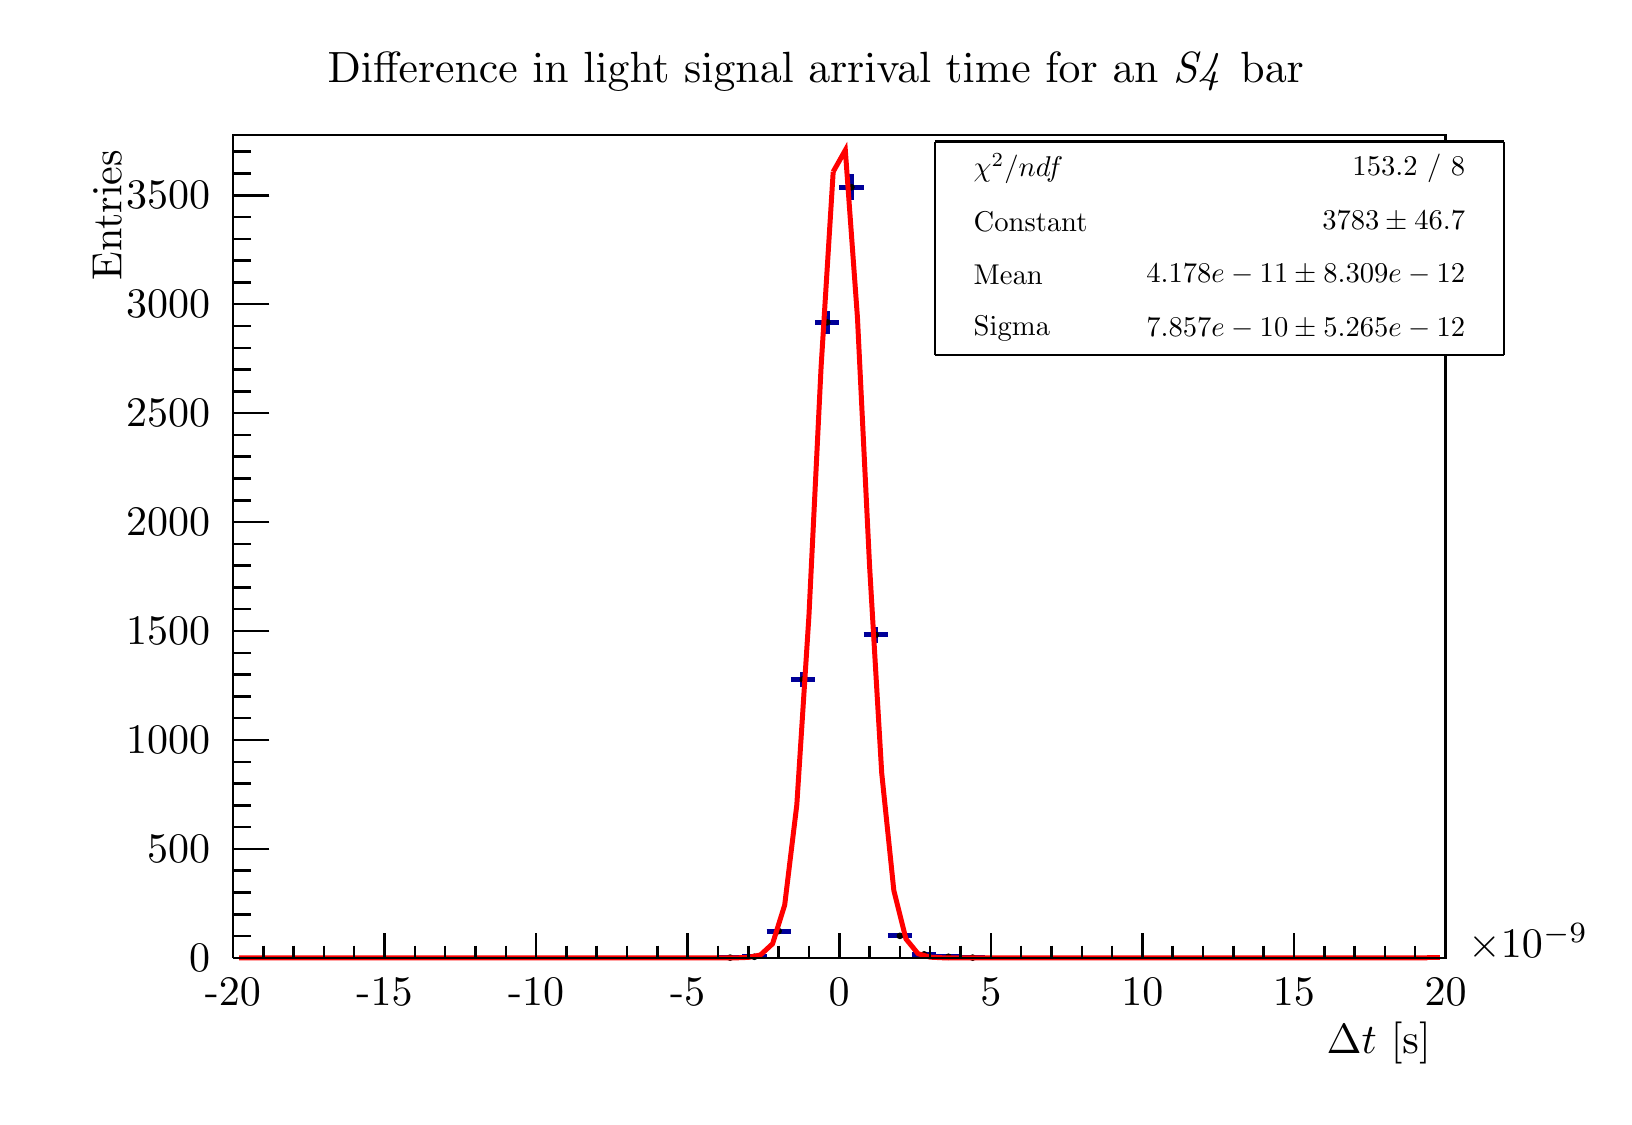
\begin{tikzpicture}
\pgfdeclareplotmark{cross} {
\pgfpathmoveto{\pgfpoint{-0.3\pgfplotmarksize}{\pgfplotmarksize}}
\pgfpathlineto{\pgfpoint{+0.3\pgfplotmarksize}{\pgfplotmarksize}}
\pgfpathlineto{\pgfpoint{+0.3\pgfplotmarksize}{0.3\pgfplotmarksize}}
\pgfpathlineto{\pgfpoint{+1\pgfplotmarksize}{0.3\pgfplotmarksize}}
\pgfpathlineto{\pgfpoint{+1\pgfplotmarksize}{-0.3\pgfplotmarksize}}
\pgfpathlineto{\pgfpoint{+0.3\pgfplotmarksize}{-0.3\pgfplotmarksize}}
\pgfpathlineto{\pgfpoint{+0.3\pgfplotmarksize}{-1.\pgfplotmarksize}}
\pgfpathlineto{\pgfpoint{-0.3\pgfplotmarksize}{-1.\pgfplotmarksize}}
\pgfpathlineto{\pgfpoint{-0.3\pgfplotmarksize}{-0.3\pgfplotmarksize}}
\pgfpathlineto{\pgfpoint{-1.\pgfplotmarksize}{-0.3\pgfplotmarksize}}
\pgfpathlineto{\pgfpoint{-1.\pgfplotmarksize}{0.3\pgfplotmarksize}}
\pgfpathlineto{\pgfpoint{-0.3\pgfplotmarksize}{0.3\pgfplotmarksize}}
\pgfpathclose
\pgfusepathqstroke
}
\pgfdeclareplotmark{cross*} {
\pgfpathmoveto{\pgfpoint{-0.3\pgfplotmarksize}{\pgfplotmarksize}}
\pgfpathlineto{\pgfpoint{+0.3\pgfplotmarksize}{\pgfplotmarksize}}
\pgfpathlineto{\pgfpoint{+0.3\pgfplotmarksize}{0.3\pgfplotmarksize}}
\pgfpathlineto{\pgfpoint{+1\pgfplotmarksize}{0.3\pgfplotmarksize}}
\pgfpathlineto{\pgfpoint{+1\pgfplotmarksize}{-0.3\pgfplotmarksize}}
\pgfpathlineto{\pgfpoint{+0.3\pgfplotmarksize}{-0.3\pgfplotmarksize}}
\pgfpathlineto{\pgfpoint{+0.3\pgfplotmarksize}{-1.\pgfplotmarksize}}
\pgfpathlineto{\pgfpoint{-0.3\pgfplotmarksize}{-1.\pgfplotmarksize}}
\pgfpathlineto{\pgfpoint{-0.3\pgfplotmarksize}{-0.3\pgfplotmarksize}}
\pgfpathlineto{\pgfpoint{-1.\pgfplotmarksize}{-0.3\pgfplotmarksize}}
\pgfpathlineto{\pgfpoint{-1.\pgfplotmarksize}{0.3\pgfplotmarksize}}
\pgfpathlineto{\pgfpoint{-0.3\pgfplotmarksize}{0.3\pgfplotmarksize}}
\pgfpathclose
\pgfusepathqfillstroke
}
\pgfdeclareplotmark{newstar} {
\pgfpathmoveto{\pgfqpoint{0pt}{\pgfplotmarksize}}
\pgfpathlineto{\pgfqpointpolar{44}{0.5\pgfplotmarksize}}
\pgfpathlineto{\pgfqpointpolar{18}{\pgfplotmarksize}}
\pgfpathlineto{\pgfqpointpolar{-20}{0.5\pgfplotmarksize}}
\pgfpathlineto{\pgfqpointpolar{-54}{\pgfplotmarksize}}
\pgfpathlineto{\pgfqpointpolar{-90}{0.5\pgfplotmarksize}}
\pgfpathlineto{\pgfqpointpolar{234}{\pgfplotmarksize}}
\pgfpathlineto{\pgfqpointpolar{198}{0.5\pgfplotmarksize}}
\pgfpathlineto{\pgfqpointpolar{162}{\pgfplotmarksize}}
\pgfpathlineto{\pgfqpointpolar{134}{0.5\pgfplotmarksize}}
\pgfpathclose
\pgfusepathqstroke
}
\pgfdeclareplotmark{newstar*} {
\pgfpathmoveto{\pgfqpoint{0pt}{\pgfplotmarksize}}
\pgfpathlineto{\pgfqpointpolar{44}{0.5\pgfplotmarksize}}
\pgfpathlineto{\pgfqpointpolar{18}{\pgfplotmarksize}}
\pgfpathlineto{\pgfqpointpolar{-20}{0.5\pgfplotmarksize}}
\pgfpathlineto{\pgfqpointpolar{-54}{\pgfplotmarksize}}
\pgfpathlineto{\pgfqpointpolar{-90}{0.5\pgfplotmarksize}}
\pgfpathlineto{\pgfqpointpolar{234}{\pgfplotmarksize}}
\pgfpathlineto{\pgfqpointpolar{198}{0.5\pgfplotmarksize}}
\pgfpathlineto{\pgfqpointpolar{162}{\pgfplotmarksize}}
\pgfpathlineto{\pgfqpointpolar{134}{0.5\pgfplotmarksize}}
\pgfpathclose
\pgfusepathqfillstroke
}
\definecolor{c}{rgb}{1,1,1};
\draw [color=c, fill=c] (0,0) rectangle (20,13.5705);
\draw [color=c, fill=c] (2.6,1.76416) rectangle (18,12.2134);
\definecolor{c}{rgb}{0,0,0};
\draw [c,line width=0.9] (2.6,1.76416) -- (2.6,12.2134) -- (18,12.2134) -- (18,1.76416) -- (2.6,1.76416);
\definecolor{c}{rgb}{1,1,1};
\draw [color=c, fill=c] (2.6,1.76416) rectangle (18,12.2134);
\definecolor{c}{rgb}{0,0,0};
\draw [c,line width=0.9] (2.6,1.76416) -- (2.6,12.2134) -- (18,12.2134) -- (18,1.76416) -- (2.6,1.76416);
\definecolor{c}{rgb}{0,0,0.6};
\draw [c,line width=1.8] (8.914,1.76416) -- (8.914,1.76693);
\draw [c,line width=1.8] (8.914,1.76693) -- (8.914,1.76969);
\draw [c,line width=1.8] (8.76,1.76693) -- (8.914,1.76693);
\draw [c,line width=1.8] (8.914,1.76693) -- (9.068,1.76693);
\definecolor{c}{rgb}{0,0,0};
\foreach \P in {(8.914,1.76693)}{\draw[mark options={color=c,fill=c},mark size=2.402402pt,mark=*,mark size=1pt] plot coordinates {\P};}
\definecolor{c}{rgb}{0,0,0.6};
\draw [c,line width=1.8] (9.222,1.77181) -- (9.222,1.77799);
\draw [c,line width=1.8] (9.222,1.77799) -- (9.222,1.78418);
\draw [c,line width=1.8] (9.068,1.77799) -- (9.222,1.77799);
\draw [c,line width=1.8] (9.222,1.77799) -- (9.376,1.77799);
\definecolor{c}{rgb}{0,0,0};
\foreach \P in {(9.222,1.77799)}{\draw[mark options={color=c,fill=c},mark size=2.402402pt,mark=*,mark size=1pt] plot coordinates {\P};}
\definecolor{c}{rgb}{0,0,0.6};
\draw [c,line width=1.8] (9.53,2.07382) -- (9.53,2.10451);
\draw [c,line width=1.8] (9.53,2.10451) -- (9.53,2.1352);
\draw [c,line width=1.8] (9.376,2.10451) -- (9.53,2.10451);
\draw [c,line width=1.8] (9.53,2.10451) -- (9.684,2.10451);
\definecolor{c}{rgb}{0,0,0};
\foreach \P in {(9.53,2.10451)}{\draw[mark options={color=c,fill=c},mark size=2.402402pt,mark=*,mark size=1pt] plot coordinates {\P};}
\definecolor{c}{rgb}{0,0,0.6};
\draw [c,line width=1.8] (9.838,5.20154) -- (9.838,5.30046);
\draw [c,line width=1.8] (9.838,5.30046) -- (9.838,5.39938);
\draw [c,line width=1.8] (9.684,5.30046) -- (9.838,5.30046);
\draw [c,line width=1.8] (9.838,5.30046) -- (9.992,5.30046);
\definecolor{c}{rgb}{0,0,0};
\foreach \P in {(9.838,5.30046)}{\draw[mark options={color=c,fill=c},mark size=2.402402pt,mark=*,mark size=1pt] plot coordinates {\P};}
\definecolor{c}{rgb}{0,0,0.6};
\draw [c,line width=1.8] (10.146,9.68623) -- (10.146,9.83568);
\draw [c,line width=1.8] (10.146,9.83568) -- (10.146,9.98513);
\draw [c,line width=1.8] (9.992,9.83568) -- (10.146,9.83568);
\draw [c,line width=1.8] (10.146,9.83568) -- (10.3,9.83568);
\definecolor{c}{rgb}{0,0,0};
\foreach \P in {(10.146,9.83568)}{\draw[mark options={color=c,fill=c},mark size=2.402402pt,mark=*,mark size=1pt] plot coordinates {\P};}
\definecolor{c}{rgb}{0,0,0.6};
\draw [c,line width=1.8] (10.454,11.3867) -- (10.454,11.5513);
\draw [c,line width=1.8] (10.454,11.5513) -- (10.454,11.7158);
\draw [c,line width=1.8] (10.3,11.5513) -- (10.454,11.5513);
\draw [c,line width=1.8] (10.454,11.5513) -- (10.608,11.5513);
\definecolor{c}{rgb}{0,0,0};
\foreach \P in {(10.454,11.5513)}{\draw[mark options={color=c,fill=c},mark size=2.402402pt,mark=*,mark size=1pt] plot coordinates {\P};}
\definecolor{c}{rgb}{0,0,0.6};
\draw [c,line width=1.8] (10.762,5.75842) -- (10.762,5.86495);
\draw [c,line width=1.8] (10.762,5.86495) -- (10.762,5.97147);
\draw [c,line width=1.8] (10.608,5.86495) -- (10.762,5.86495);
\draw [c,line width=1.8] (10.762,5.86495) -- (10.916,5.86495);
\definecolor{c}{rgb}{0,0,0};
\foreach \P in {(10.762,5.86495)}{\draw[mark options={color=c,fill=c},mark size=2.402402pt,mark=*,mark size=1pt] plot coordinates {\P};}
\definecolor{c}{rgb}{0,0,0.6};
\draw [c,line width=1.8] (11.07,2.01582) -- (11.07,2.04363);
\draw [c,line width=1.8] (11.07,2.04363) -- (11.07,2.07144);
\draw [c,line width=1.8] (10.916,2.04363) -- (11.07,2.04363);
\draw [c,line width=1.8] (11.07,2.04363) -- (11.224,2.04363);
\definecolor{c}{rgb}{0,0,0};
\foreach \P in {(11.07,2.04363)}{\draw[mark options={color=c,fill=c},mark size=2.402402pt,mark=*,mark size=1pt] plot coordinates {\P};}
\definecolor{c}{rgb}{0,0,0.6};
\draw [c,line width=1.8] (11.378,1.79736) -- (11.378,1.80843);
\draw [c,line width=1.8] (11.378,1.80843) -- (11.378,1.8195);
\draw [c,line width=1.8] (11.224,1.80843) -- (11.378,1.80843);
\draw [c,line width=1.8] (11.378,1.80843) -- (11.532,1.80843);
\definecolor{c}{rgb}{0,0,0};
\foreach \P in {(11.378,1.80843)}{\draw[mark options={color=c,fill=c},mark size=2.402402pt,mark=*,mark size=1pt] plot coordinates {\P};}
\definecolor{c}{rgb}{0,0,0.6};
\draw [c,line width=1.8] (11.686,1.77181) -- (11.686,1.77799);
\draw [c,line width=1.8] (11.686,1.77799) -- (11.686,1.78418);
\draw [c,line width=1.8] (11.532,1.77799) -- (11.686,1.77799);
\draw [c,line width=1.8] (11.686,1.77799) -- (11.84,1.77799);
\definecolor{c}{rgb}{0,0,0};
\foreach \P in {(11.686,1.77799)}{\draw[mark options={color=c,fill=c},mark size=2.402402pt,mark=*,mark size=1pt] plot coordinates {\P};}
\definecolor{c}{rgb}{0,0,0.6};
\draw [c,line width=1.8] (11.994,1.76416) -- (11.994,1.76693);
\draw [c,line width=1.8] (11.994,1.76693) -- (11.994,1.76969);
\draw [c,line width=1.8] (11.84,1.76693) -- (11.994,1.76693);
\draw [c,line width=1.8] (11.994,1.76693) -- (12.148,1.76693);
\definecolor{c}{rgb}{0,0,0};
\foreach \P in {(11.994,1.76693)}{\draw[mark options={color=c,fill=c},mark size=2.402402pt,mark=*,mark size=1pt] plot coordinates {\P};}
\definecolor{c}{rgb}{1,0,0};
\draw [c,line width=1.8] (2.677,1.76416) -- (2.831,1.76416) -- (2.985,1.76416) -- (3.139,1.76416) -- (3.293,1.76416) -- (3.447,1.76416) -- (3.601,1.76416) -- (3.755,1.76416) -- (3.909,1.76416) -- (4.063,1.76416) -- (4.217,1.76416) -- (4.371,1.76416)
 -- (4.525,1.76416) -- (4.679,1.76416) -- (4.833,1.76416) -- (4.987,1.76416) -- (5.141,1.76416) -- (5.295,1.76416) -- (5.449,1.76416) -- (5.603,1.76416) -- (5.757,1.76416) -- (5.911,1.76416) -- (6.065,1.76416) -- (6.219,1.76416) -- (6.373,1.76416) --
 (6.527,1.76416) -- (6.681,1.76416) -- (6.835,1.76416) -- (6.989,1.76416) -- (7.143,1.76416) -- (7.297,1.76416) -- (7.451,1.76416) -- (7.605,1.76416) -- (7.759,1.76416) -- (7.913,1.76416) -- (8.067,1.76416) -- (8.221,1.76416) -- (8.375,1.76416) --
 (8.529,1.76416) -- (8.683,1.76416) -- (8.837,1.76416) -- (8.991,1.76416) -- (9.145,1.76998) -- (9.299,1.80089) -- (9.453,1.94285) -- (9.607,2.43506) -- (9.761,3.70796) -- (9.915,6.11015) -- (10.069,9.26248) -- (10.223,11.7476);
\draw [c,line width=1.8] (10.223,11.7476) -- (10.377,12.0215) -- (10.531,9.89679) -- (10.685,6.74) -- (10.839,4.11347) -- (10.993,2.62012) -- (11.147,2.00482) -- (11.301,1.81637) -- (11.455,1.7729) -- (11.609,1.76529) -- (11.763,1.76416) --
 (11.917,1.76416) -- (12.071,1.76416) -- (12.225,1.76416) -- (12.379,1.76416) -- (12.533,1.76416) -- (12.687,1.76416) -- (12.841,1.76416) -- (12.995,1.76416) -- (13.149,1.76416) -- (13.303,1.76416) -- (13.457,1.76416) -- (13.611,1.76416) --
 (13.765,1.76416) -- (13.919,1.76416) -- (14.073,1.76416) -- (14.227,1.76416) -- (14.381,1.76416) -- (14.535,1.76416) -- (14.689,1.76416) -- (14.843,1.76416) -- (14.997,1.76416) -- (15.151,1.76416) -- (15.305,1.76416) -- (15.459,1.76416) --
 (15.613,1.76416) -- (15.767,1.76416) -- (15.921,1.76416) -- (16.075,1.76416) -- (16.229,1.76416) -- (16.383,1.76416) -- (16.537,1.76416) -- (16.691,1.76416) -- (16.845,1.76416) -- (16.999,1.76416) -- (17.153,1.76416) -- (17.307,1.76416) --
 (17.461,1.76416) -- (17.615,1.76416) -- (17.769,1.76416);
\draw [c,line width=1.8] (17.769,1.76416) -- (17.923,1.76416);
\definecolor{c}{rgb}{1,1,1};
\draw [color=c, fill=c] (11.5186,9.42152) rectangle (18.7393,12.1299);
\definecolor{c}{rgb}{0,0,0};
\draw [c,line width=0.9] (11.5186,9.42152) -- (18.7393,9.42152);
\draw [c,line width=0.9] (18.7393,9.42152) -- (18.7393,12.1299);
\draw [c,line width=0.9] (18.7393,12.1299) -- (11.5186,12.1299);
\draw [c,line width=0.9] (11.5186,12.1299) -- (11.5186,9.42152);
\draw [anchor= west] (11.8797,11.7913) node[scale=1.03301, color=c, rotate=0]{$\chi^{2} / ndf $};
\draw [anchor= east] (18.3782,11.7913) node[scale=1.03301, color=c, rotate=0]{ 153.2 / 8};
\draw [anchor= west] (11.8797,11.1142) node[scale=1.03301, color=c, rotate=0]{Constant };
\draw [anchor= east] (18.3782,11.1142) node[scale=1.03301, color=c, rotate=0]{$  3783 \pm 46.7$};
\draw [anchor= west] (11.8797,10.4371) node[scale=1.03301, color=c, rotate=0]{Mean     };
\draw [anchor= east] (18.3782,10.4371) node[scale=1.03301, color=c, rotate=0]{$ 4.178e-11 \pm 8.309e-12$};
\draw [anchor= west] (11.8797,9.76007) node[scale=1.03301, color=c, rotate=0]{Sigma    };
\draw [anchor= east] (18.3782,9.76007) node[scale=1.03301, color=c, rotate=0]{$ 7.857e-10 \pm 5.265e-12$};
\draw [c,line width=0.9] (2.6,1.76416) -- (18,1.76416);
\draw [c,line width=0.9] (2.6,2.07764) -- (2.6,1.76416);
\draw [c,line width=0.9] (2.985,1.9209) -- (2.985,1.76416);
\draw [c,line width=0.9] (3.37,1.9209) -- (3.37,1.76416);
\draw [c,line width=0.9] (3.755,1.9209) -- (3.755,1.76416);
\draw [c,line width=0.9] (4.14,1.9209) -- (4.14,1.76416);
\draw [c,line width=0.9] (4.525,2.07764) -- (4.525,1.76416);
\draw [c,line width=0.9] (4.91,1.9209) -- (4.91,1.76416);
\draw [c,line width=0.9] (5.295,1.9209) -- (5.295,1.76416);
\draw [c,line width=0.9] (5.68,1.9209) -- (5.68,1.76416);
\draw [c,line width=0.9] (6.065,1.9209) -- (6.065,1.76416);
\draw [c,line width=0.9] (6.45,2.07764) -- (6.45,1.76416);
\draw [c,line width=0.9] (6.835,1.9209) -- (6.835,1.76416);
\draw [c,line width=0.9] (7.22,1.9209) -- (7.22,1.76416);
\draw [c,line width=0.9] (7.605,1.9209) -- (7.605,1.76416);
\draw [c,line width=0.9] (7.99,1.9209) -- (7.99,1.76416);
\draw [c,line width=0.9] (8.375,2.07764) -- (8.375,1.76416);
\draw [c,line width=0.9] (8.76,1.9209) -- (8.76,1.76416);
\draw [c,line width=0.9] (9.145,1.9209) -- (9.145,1.76416);
\draw [c,line width=0.9] (9.53,1.9209) -- (9.53,1.76416);
\draw [c,line width=0.9] (9.915,1.9209) -- (9.915,1.76416);
\draw [c,line width=0.9] (10.3,2.07764) -- (10.3,1.76416);
\draw [c,line width=0.9] (10.685,1.9209) -- (10.685,1.76416);
\draw [c,line width=0.9] (11.07,1.9209) -- (11.07,1.76416);
\draw [c,line width=0.9] (11.455,1.9209) -- (11.455,1.76416);
\draw [c,line width=0.9] (11.84,1.9209) -- (11.84,1.76416);
\draw [c,line width=0.9] (12.225,2.07764) -- (12.225,1.76416);
\draw [c,line width=0.9] (12.61,1.9209) -- (12.61,1.76416);
\draw [c,line width=0.9] (12.995,1.9209) -- (12.995,1.76416);
\draw [c,line width=0.9] (13.38,1.9209) -- (13.38,1.76416);
\draw [c,line width=0.9] (13.765,1.9209) -- (13.765,1.76416);
\draw [c,line width=0.9] (14.15,2.07764) -- (14.15,1.76416);
\draw [c,line width=0.9] (14.535,1.9209) -- (14.535,1.76416);
\draw [c,line width=0.9] (14.92,1.9209) -- (14.92,1.76416);
\draw [c,line width=0.9] (15.305,1.9209) -- (15.305,1.76416);
\draw [c,line width=0.9] (15.69,1.9209) -- (15.69,1.76416);
\draw [c,line width=0.9] (16.075,2.07764) -- (16.075,1.76416);
\draw [c,line width=0.9] (16.46,1.9209) -- (16.46,1.76416);
\draw [c,line width=0.9] (16.845,1.9209) -- (16.845,1.76416);
\draw [c,line width=0.9] (17.23,1.9209) -- (17.23,1.76416);
\draw [c,line width=0.9] (17.615,1.9209) -- (17.615,1.76416);
\draw [c,line width=0.9] (18,2.07764) -- (18,1.76416);
\draw [anchor=base] (2.6,1.15349) node[scale=1.51913, color=c, rotate=0]{-20};
\draw [anchor=base] (4.525,1.15349) node[scale=1.51913, color=c, rotate=0]{-15};
\draw [anchor=base] (6.45,1.15349) node[scale=1.51913, color=c, rotate=0]{-10};
\draw [anchor=base] (8.375,1.15349) node[scale=1.51913, color=c, rotate=0]{-5};
\draw [anchor=base] (10.3,1.15349) node[scale=1.51913, color=c, rotate=0]{0};
\draw [anchor=base] (12.225,1.15349) node[scale=1.51913, color=c, rotate=0]{5};
\draw [anchor=base] (14.15,1.15349) node[scale=1.51913, color=c, rotate=0]{10};
\draw [anchor=base] (16.075,1.15349) node[scale=1.51913, color=c, rotate=0]{15};
\draw [anchor=base] (18,1.15349) node[scale=1.51913, color=c, rotate=0]{20};
\draw [anchor=base west] (18.1,1.76416) node[scale=1.51913, color=c, rotate=0]{$\times10^{-9}$};
\draw [anchor= east] (18,0.678523) node[scale=1.51913, color=c, rotate=0]{$\Delta t$ [s]};
\draw [c,line width=0.9] (2.6,1.76416) -- (2.6,12.2134);
\draw [c,line width=0.9] (3.062,1.76416) -- (2.6,1.76416);
\draw [c,line width=0.9] (2.831,2.04086) -- (2.6,2.04086);
\draw [c,line width=0.9] (2.831,2.31757) -- (2.6,2.31757);
\draw [c,line width=0.9] (2.831,2.59428) -- (2.6,2.59428);
\draw [c,line width=0.9] (2.831,2.87098) -- (2.6,2.87098);
\draw [c,line width=0.9] (3.062,3.14769) -- (2.6,3.14769);
\draw [c,line width=0.9] (2.831,3.4244) -- (2.6,3.4244);
\draw [c,line width=0.9] (2.831,3.7011) -- (2.6,3.7011);
\draw [c,line width=0.9] (2.831,3.97781) -- (2.6,3.97781);
\draw [c,line width=0.9] (2.831,4.25451) -- (2.6,4.25451);
\draw [c,line width=0.9] (3.062,4.53122) -- (2.6,4.53122);
\draw [c,line width=0.9] (2.831,4.80793) -- (2.6,4.80793);
\draw [c,line width=0.9] (2.831,5.08463) -- (2.6,5.08463);
\draw [c,line width=0.9] (2.831,5.36134) -- (2.6,5.36134);
\draw [c,line width=0.9] (2.831,5.63805) -- (2.6,5.63805);
\draw [c,line width=0.9] (3.062,5.91475) -- (2.6,5.91475);
\draw [c,line width=0.9] (2.831,6.19146) -- (2.6,6.19146);
\draw [c,line width=0.9] (2.831,6.46816) -- (2.6,6.46816);
\draw [c,line width=0.9] (2.831,6.74487) -- (2.6,6.74487);
\draw [c,line width=0.9] (2.831,7.02158) -- (2.6,7.02158);
\draw [c,line width=0.9] (3.062,7.29828) -- (2.6,7.29828);
\draw [c,line width=0.9] (2.831,7.57499) -- (2.6,7.57499);
\draw [c,line width=0.9] (2.831,7.8517) -- (2.6,7.8517);
\draw [c,line width=0.9] (2.831,8.1284) -- (2.6,8.1284);
\draw [c,line width=0.9] (2.831,8.40511) -- (2.6,8.40511);
\draw [c,line width=0.9] (3.062,8.68182) -- (2.6,8.68182);
\draw [c,line width=0.9] (2.831,8.95852) -- (2.6,8.95852);
\draw [c,line width=0.9] (2.831,9.23523) -- (2.6,9.23523);
\draw [c,line width=0.9] (2.831,9.51193) -- (2.6,9.51193);
\draw [c,line width=0.9] (2.831,9.78864) -- (2.6,9.78864);
\draw [c,line width=0.9] (3.062,10.0653) -- (2.6,10.0653);
\draw [c,line width=0.9] (2.831,10.3421) -- (2.6,10.3421);
\draw [c,line width=0.9] (2.831,10.6188) -- (2.6,10.6188);
\draw [c,line width=0.9] (2.831,10.8955) -- (2.6,10.8955);
\draw [c,line width=0.9] (2.831,11.1722) -- (2.6,11.1722);
\draw [c,line width=0.9] (3.062,11.4489) -- (2.6,11.4489);
\draw [c,line width=0.9] (3.062,11.4489) -- (2.6,11.4489);
\draw [c,line width=0.9] (2.831,11.7256) -- (2.6,11.7256);
\draw [c,line width=0.9] (2.831,12.0023) -- (2.6,12.0023);
\draw [anchor= east] (2.5,1.76416) node[scale=1.51913, color=c, rotate=0]{0};
\draw [anchor= east] (2.5,3.14769) node[scale=1.51913, color=c, rotate=0]{500};
\draw [anchor= east] (2.5,4.53122) node[scale=1.51913, color=c, rotate=0]{1000};
\draw [anchor= east] (2.5,5.91475) node[scale=1.51913, color=c, rotate=0]{1500};
\draw [anchor= east] (2.5,7.29828) node[scale=1.51913, color=c, rotate=0]{2000};
\draw [anchor= east] (2.5,8.68182) node[scale=1.51913, color=c, rotate=0]{2500};
\draw [anchor= east] (2.5,10.0653) node[scale=1.51913, color=c, rotate=0]{3000};
\draw [anchor= east] (2.5,11.4489) node[scale=1.51913, color=c, rotate=0]{3500};
\draw [anchor= east] (1,12.2134) node[scale=1.51913, color=c, rotate=90]{Entries};
\definecolor{c}{rgb}{1,1,1};
\draw [color=c, fill=c] (11.5186,9.42152) rectangle (18.7393,12.1299);
\definecolor{c}{rgb}{0,0,0};
\draw [c,line width=0.9] (11.5186,9.42152) -- (18.7393,9.42152);
\draw [c,line width=0.9] (18.7393,9.42152) -- (18.7393,12.1299);
\draw [c,line width=0.9] (18.7393,12.1299) -- (11.5186,12.1299);
\draw [c,line width=0.9] (11.5186,12.1299) -- (11.5186,9.42152);
\draw [anchor= west] (11.8797,11.7913) node[scale=1.03301, color=c, rotate=0]{$\chi^{2} / ndf $};
\draw [anchor= east] (18.3782,11.7913) node[scale=1.03301, color=c, rotate=0]{ 153.2 / 8};
\draw [anchor= west] (11.8797,11.1142) node[scale=1.03301, color=c, rotate=0]{Constant };
\draw [anchor= east] (18.3782,11.1142) node[scale=1.03301, color=c, rotate=0]{$  3783 \pm 46.7$};
\draw [anchor= west] (11.8797,10.4371) node[scale=1.03301, color=c, rotate=0]{Mean     };
\draw [anchor= east] (18.3782,10.4371) node[scale=1.03301, color=c, rotate=0]{$ 4.178e-11 \pm 8.309e-12$};
\draw [anchor= west] (11.8797,9.76007) node[scale=1.03301, color=c, rotate=0]{Sigma    };
\draw [anchor= east] (18.3782,9.76007) node[scale=1.03301, color=c, rotate=0]{$ 7.857e-10 \pm 5.265e-12$};
\draw (10,13.0186) node[scale=1.5799, color=c, rotate=0]{Difference in light signal arrival time for an $\mathit{S4}$ bar};
\end{tikzpicture}

  \end{adjustbox}
  \caption{Difference in signal arrival time for PMTs at each end of a bar as measured using a $^{90}$Sr source placed 64~cm from one end of the bar.}
  \label{fig:s4Res}	
\end{figure}

%\begin{figure}[ht]    
 % \centering
 %% 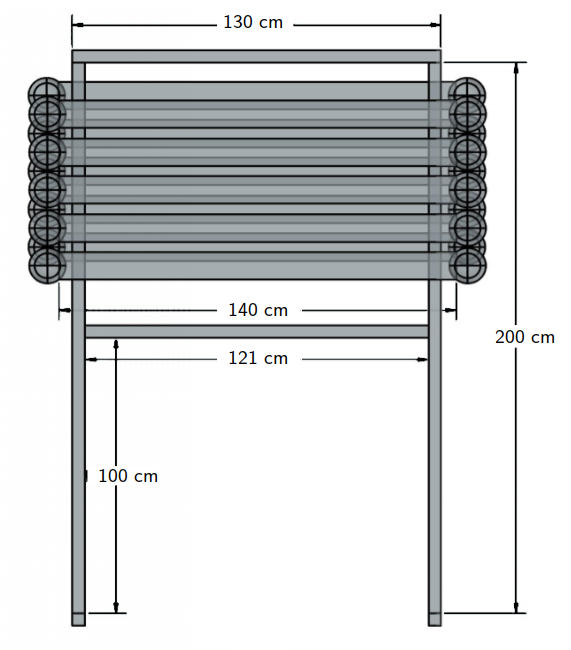
\includegraphics[width=0.5\linewidth]{files/Figures/dstofFront2.png}
  %\hfill
  %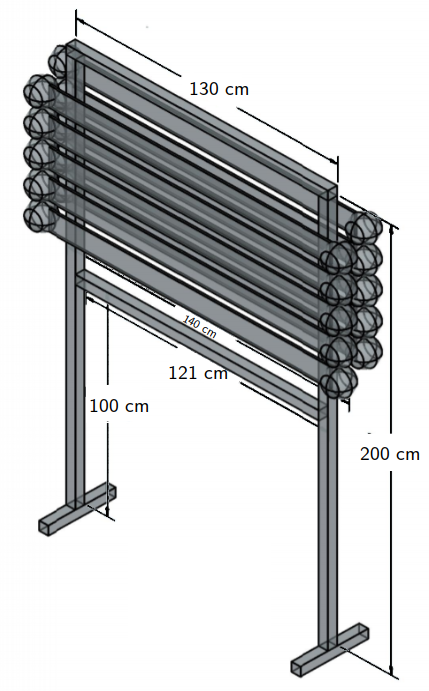
\includegraphics[width=0.35\linewidth]{files/Figures/dstofDiag2.png}
  %\caption{Front (left) and rotated (right) view of the $\mathit{S4}$ panel. The rotated view shows more clearly the staggering of the scintillator bars and PMTs.}
 % \label{fig:dstofDiagram}
%\end{figure}

The anode signals of all 20 of the PMTs are discriminated using LeCroy 620AL NIM discriminators, at a threshold of 20~mV.
The discriminated signals are then fed into a time-to-digital converter (TDC). A signal in $\mathit{S4}$ is deemed to have occurred if a signal is seen in both PMTs, above the discriminator threshold, on the same bar within 20~ns of each other. 
This timing window is determined through testing performed with a $^{90}$Sr source at known positions on the bar.

The $\mathit{S1-S2}$ coincidence signal is digitized by the same TDC. This signal is used to calculate the particle time of flight from $\mathit{S2}$ to $\mathit{S4}$.

\subsection{The HPTPC Prototype}
For the characterisation of the beam using the ToF systems described in this paper, the relevant characteristics of the HPTPC prototype are the location and thickness of the steel vessel walls.
The cylindrical steel vessel has a 142~cm outer diameter; the main body is 60 cm in length and the rounded end caps protrude an additional 37~cm on each end.
With 1~cm thick walls it is rated to 6~bar of absolute pressure.
The vessel wall thickness is equivalent to the range of a proton with a kinetic energy of approximately 80~MeV~\cite{rangeTables}.
For the unmoderated beam, the typical energy loss of a proton which does not stop in the vessel is 50~MeV.
This is determined from the Monte Carlo studies detailed in Section~\ref{sec:mcStudies}.
The angular position of the center of the TPC is approximately $\theta = -2.5^{\circ}$. 
More details of the position and extent of the TPC are given in Table~\ref{tab:angS1} and Table~\ref{tab:distances}.
 
The active TPC is a cylinder, 111~cm in diameter and 48~cm in length; the TPC comprised thin steel mesh electrodes (one cathode with \SI{118}{\centi\meter} diameter and three anodes with \SI{121}{\centi\meter} diameter), and 12 copper rings to create the uniform drift field. The anodes were supported by a hexagonal aluminium stiffener on the side facing away from the camera.
Data taking with the TPC made use of both optical and charge readout.
The vessel, electrodes, and drift region of the TPC are shown in Figure~\ref{fig:TPC}.

\begin{figure}
  \centering
  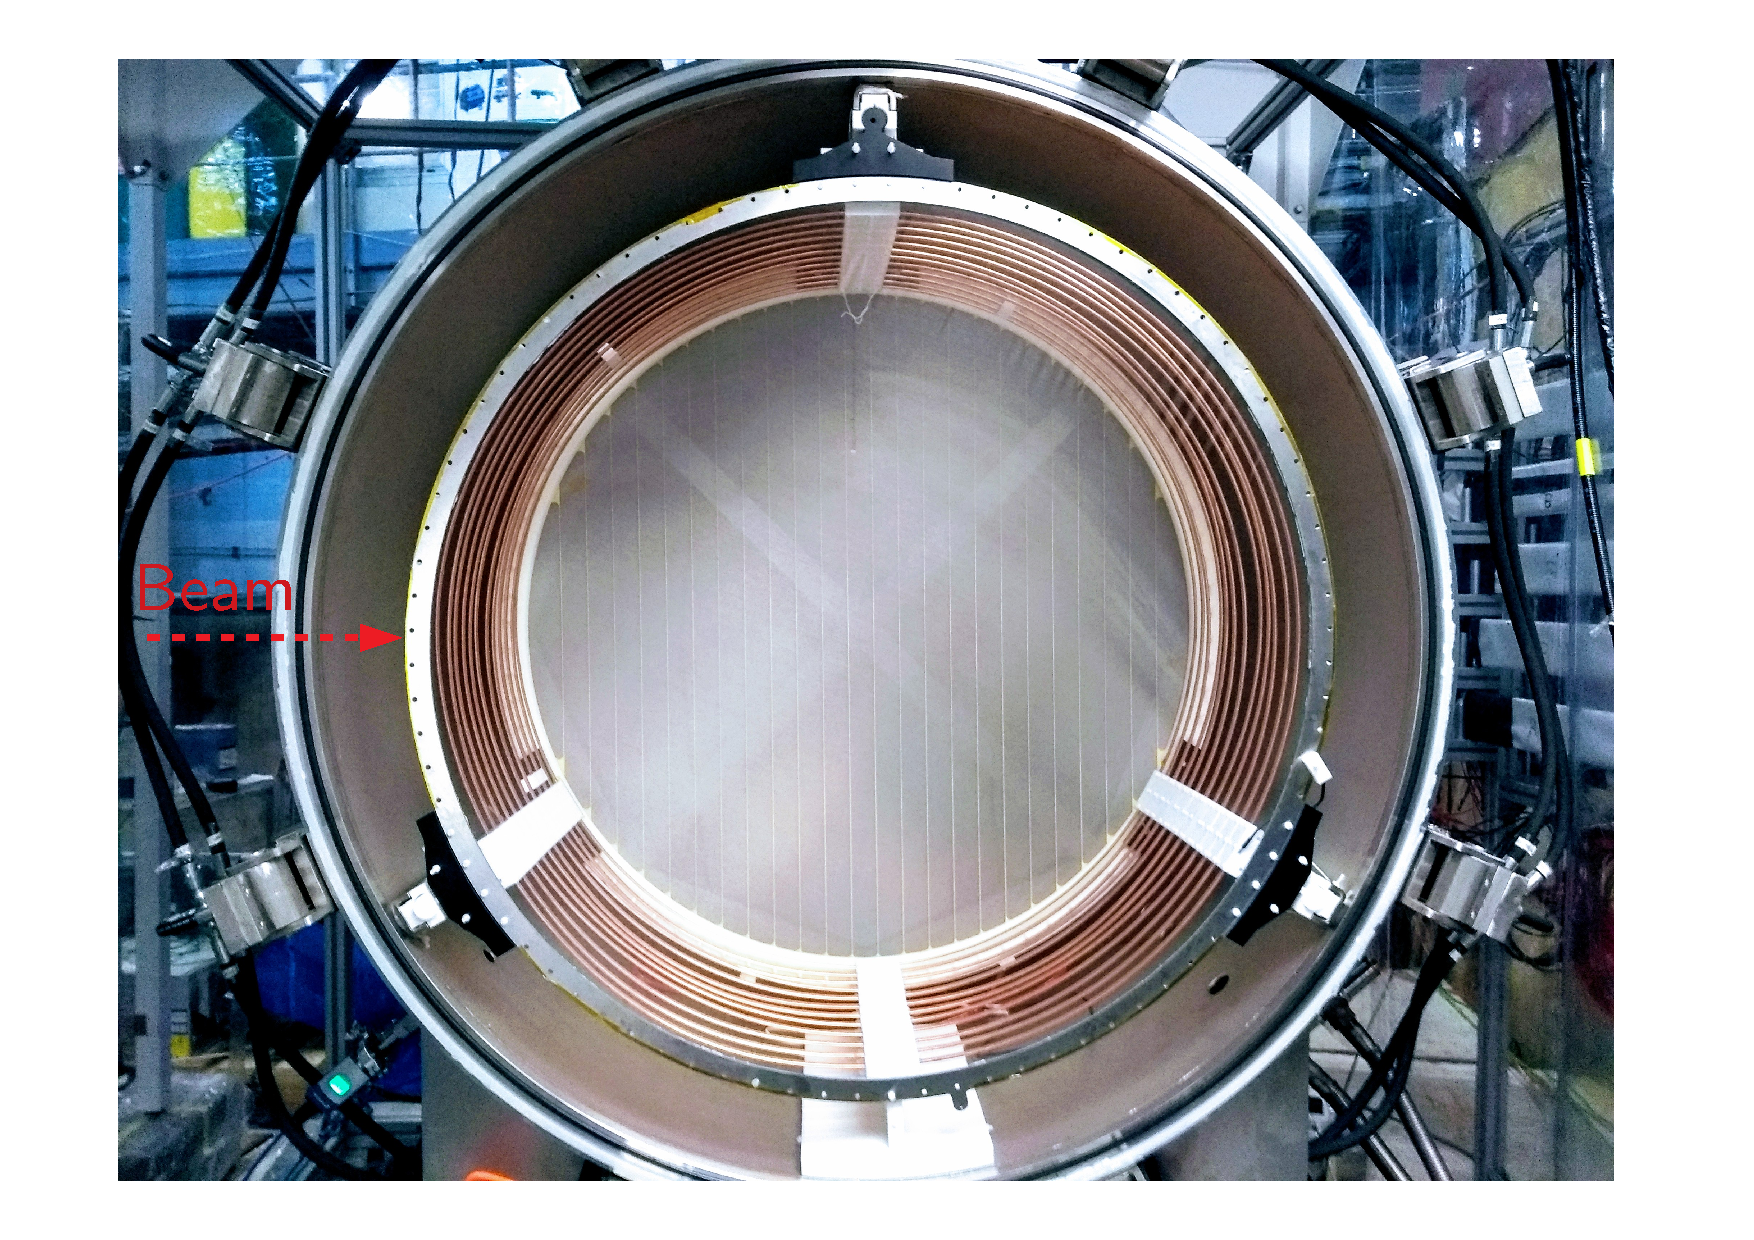
\includegraphics[width=.8\linewidth]{files/Figures/vesselView.pdf}
  \caption{Cross-sectional view of the TPC; the thin mesh electrodes and copper ring drift volume can be seen inside the steel vessel. The walls of the vessel shown are 1~cm thick with a vessel outer diameter of 142~cm. At the point of hitting the vessel, the beam centre was 1~cm below the centre of the vessel vertically, where the distance from the inside of the vessel wall to the drift region was 15~cm.}
   \label{fig:TPC}
   %Vessel: wall thickness 1cm, beam centre height -1.14cm, 
\end{figure}

Throughout the run, the TPC was filled with either pure argon, or a combination of argon and a small percentage of quencher.
The performance of this TPC is the subject of a forthcoming publication~\cite{Deisting:2020aaa}.
